
%%%%%%%%%%%%%%%%%%%%%%%%%%%%%%%%%%%%%%%%%%%%%%%%%%%%%%%%%%%%%%%%%%%%%%%%%%%%%%%
%
%  EGSnrc user codes manual
%  Copyright (C) 2021 National Research Council Canada
%
%  This file is part of EGSnrc.
%
%  EGSnrc is free software: you can redistribute it and/or modify it under
%  the terms of the GNU Affero General Public License as published by the
%  Free Software Foundation, either version 3 of the License, or (at your
%  option) any later version.
%
%  EGSnrc is distributed in the hope that it will be useful, but WITHOUT ANY
%  WARRANTY; without even the implied warranty of MERCHANTABILITY or FITNESS
%  FOR A PARTICULAR PURPOSE.  See the GNU Affero General Public License for
%  more details.
%
%  You should have received a copy of the GNU Affero General Public License
%  along with EGSnrc. If not, see <http://www.gnu.org/licenses/>.
%
%%%%%%%%%%%%%%%%%%%%%%%%%%%%%%%%%%%%%%%%%%%%%%%%%%%%%%%%%%%%%%%%%%%%%%%%%%%%%%%
%
%  Authors:         Dave Rogers
%                   Iwan Kawrakow
%                   Jan Seuntjens
%                   Blake Walters
%                   Ernesto Mainegra-Hing
%
%  Contributors:    Frederic Tessier
%
%%%%%%%%%%%%%%%%%%%%%%%%%%%%%%%%%%%%%%%%%%%%%%%%%%%%%%%%%%%%%%%%%%%%%%%%%%%%%%%


\documentclass[12pt,twoside]{article}  %indexm doesn't work with two
					%sides
%\usepackage{supertab}%this didn't work for some reason?
%\usepackage{overcite}			%comment out for html?

\usepackage{moreverb}	%this is used for the boxedverbatim environment
			%used to box the listing files for tutor programs

\setlength{\textwidth}{16.51cm}
%\setlength{\textheight}{23.2cm}
\setlength{\textheight}{23.5cm}
\setlength{\oddsidemargin}{0.0in}
\setlength{\evensidemargin}{0.0in}
\setlength{\topmargin}{-1.5cm}
\setlength{\parindent}{1.5em}
\setlength{\topsep}{0ex}
\setlength{\itemsep}{0ex}

\newcommand{\lpage}[1]{(page~\pageref{#1})}
\newcommand{\Mol}{Moli\`ere}

\newcommand{\Co}{$^{60}$Co}
\newcommand{\parsp}{~\hspace*{1.5em}}
\setlength{\parskip}{0.1in}
\setlength{\baselineskip}{1.0cm}
\newcommand{\head}[1]{\begin{center}\begin{Large}{\bf #1}
                                              \end{Large}\end{center}}
\newcommand{\cen}[1]{\begin{center} #1 \end{center} }
\newcommand{\etal}{{\em et.al.}}
\newcommand{\ie}{{\em i.e.}}
\newcommand{\etc}{{\em etc.}}
\newcommand{\viz}{{\em viz.}}
\newcommand{\eg}{{\em eg.}}
\newcommand{\sprt}[2]{\left(\frac{\overline{L}}{\rho}\right)^{\rm #1}_{\rm #2}}
\newcommand{\eqn}[1]{\begin{equation} #1 \end{equation} }
\newcommand{\rsp}[1]{\left( \frac{L(\Delta)}{\rho} \right)_{#1}}
\newcommand{\PhiT}{\Phi_{\rm T}}
\newcommand{\rspt}[1]{\left( \frac{S(\Delta)}{\rho} \right)_{#1}}
\newcommand{\rspE}[2]{\left( \frac{L({\rm #1})}{\rho} \right)_{#2}}

\newcommand{\note}[1]{\mbox{}\\ \noindent \rule{16cm}{0.5mm} \\
{\em #1} \\ \noindent \rule{16cm}{0.5mm}\\
\typeout{******note: #1 *****}
}

%\newcommand{\indexm}[1]{\index{#1}}
%\typeout{~~~~~~~~~~~~***margin index feature OFF*****************************}
%\typeout{~~~~~~~~~~~~***margin index feature OFF*****************************}
%\typeout{~~~~~~~~~~~~***margin index feature OFF*****************************}
\newcommand{\indexm}[1]{\marginpar{{\sf {\tiny I:#1} }}\index{#1}}
\makeindex


\renewcommand{\refname}{}

%       some commands to get 4 levels in the table of contents and
%       number down to paragraphs
\setcounter{secnumdepth}{4}
\setcounter{tocdepth}{4}
\renewcommand{\thesubsubsection}{\thesubsection.\arabic{subsubsection}}
\renewcommand{\theparagraph}{\thesubsubsection.\roman{paragraph}}
%\renewcommand{\theequation}{\arabic{subsection}.\arabic{subsubsection}.\arabic{equation}}



%\usepackage{html}
\usepackage{graphicx}
%\usepackage{epsf}
%\input{epsf}
\usepackage{longtable}

\usepackage{fancyhdr}
\renewcommand{\footrulewidth}{0.4pt}
\renewcommand{\headrulewidth}{0.4pt}

\lhead[{\sffamily \thepage}]{{\sffamily NRC User Codes for EGSnrc }}
\rhead[{\sffamily NRCC Report PIRS-702}]{{\sffamily ~\thepage}}
%\rfoot[{\sffamily {\rightmark}}]{{\sffamily {\rightmark}}}
\rfoot[]{{\sffamily {\rightmark}}}
% \lfoot[{\sffamily {\leftmark}}]{{\small Last edited $Date: 2013/09/24 18:04:14 $
\lfoot[{\sffamily {\leftmark}}]{{\small Last edited 2011/05/03 15:50:14
}}
\cfoot{}

\usepackage{hyperref}
\hypersetup{colorlinks=true, citecolor=blue, linkcolor=blue, filecolor=blue, urlcolor=blue}
\urlstyle{same}

\usepackage{html}



\begin{latexonly}
\typeout{***Have turned off overfull and underfull messages****}
\tolerance=10000        %suppress Overfull only
\hbadness=10000         %suppress Overfull and Underfull for text (horizontal)
\vbadness=10000         %suppress Overfull and Underfull for vertical "boxes"
\end{latexonly}


\begin{document}

\begin{htmlonly}
For information about the authors and/or institutions involved with this
work, use the links provided in the author list.\\

\begin{rawhtml}
<br><br>
\end{rawhtml}


Postscript versions of the entire paper are available.  You may have to
download the compressed version to disk, uncompress or gunzip them and
then read or print them.\\
\begin{center}
\htmladdnormallink{(uncompressed version 2.4 Mb)}{pirs702.ps}\\
\htmladdnormallink{(gzip version 230 kb)}{pirs702.ps.gz}\\
\htmladdnormallink{(pdf version 440 kb)}{pirs702.pdf}\\
\end{center}
\begin{rawhtml}
<br><br>
\end{rawhtml}

Use the Up button to get back to this page from within the document.
\begin{rawhtml}
<BR> <HR> <P>
\end{rawhtml}
\copyright
Copyright 2021,  National Research Council of Canada
Ottawa
\begin{rawhtml}
<BR> <HR> <P>
\end{rawhtml}
\end{htmlonly}

\pagestyle{empty}

\title{NRC User Codes for EGSnrc}

\begin{center}
{\sffamily \bfseries {\Huge NRC User Codes for EGSnrc}
\vspace{5mm}\\}
\begin{Large}
D.W.O. Rogers, I. Kawrakow, J.P. Seuntjens,  B.R.B. Walters and E.
Mainegra-Hing \\
\end{Large}
Ionizing Radiation Standards,
National Research Council Canada, Ottawa, Canada\\


\vspace{3mm}
{\bfseries
\today}
%January 2010}
\vspace{3mm}\\
\hfill NRCC Report {\sf PIRS-702(revC)} \vspace*{2mm}\\

\begin{figure}[h]
\htmlimage{scale=1.2}{}
\begin{center}
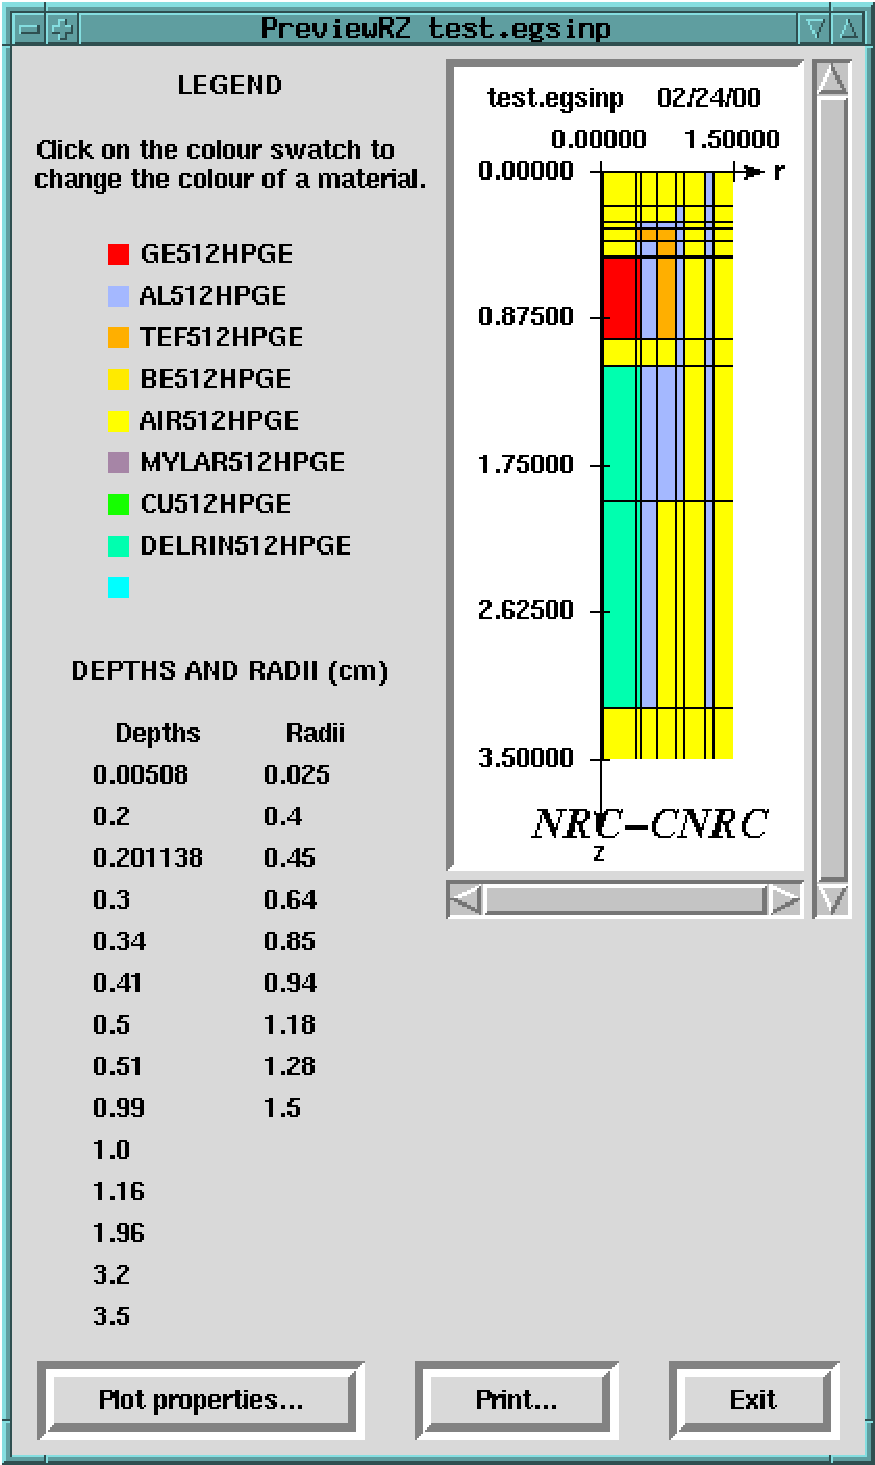
\includegraphics[height=12cm]{figures/PreviewRZ_example}
\\Preview of an RZ geometry in DOSRZnrc.
\end{center}
%\caption{Preview of an RZ geometry in DOSRZnrc.}
%\cen{Get a figure from preview tcl of DOSRZnrc}
\end{figure}

\vfill
\begin{latexonly}
\end{latexonly}

\copyright NRC Canada, 2021
\end{center}
\newpage   %Blank page behind cover
\mbox{}

%\note{This page is intentionally blank to be the back of the front cover.
%Remove this note prior to printing!!!}

\setlength{\baselineskip}{0.5cm}
\newpage

\pagestyle{fancy}
\pagenumbering{arabic}
\setcounter{page}{1}


\begin{abstract}
\label{abstract}
This manual describes the NRC User codes DOSRZnrc, CAVRZnrc, FLURZnrc and
SPRRZnrc which all work with the EGSnrc Code system for Monte Carlo
transport of electrons and photons (see NRC REPORT PIRS--701, ``The EGSnrc
Code System''). There is a graphical user interface available for creating
the inputs to these codes (described separately).

\end{abstract}

%\newpage

\setlength{\baselineskip}{0.1cm}

\tableofcontents

%\newpage
\listoftables
\listoffigures

\setlength{\baselineskip}{0.5cm}

\newpage

\renewcommand{\leftmark}{{INTRODUCTION}}
\section{Introduction}
\subsection{Intent of this report}

Over the years, NRC has developed and distributed a series of user codes
for use with the EGS4 code system for the Monte Carlo simulation of photon
and electron transport.  These have been widely used and their results
compared to experiment in many cases.  However, the codes themselves have
never been properly documented and described. It is the purpose of this
manual to provide a document which describes
both how these codes work and also how a user uses them.  It is not the
purpose of this manual to discuss selection of parameters when using these
codes for a particular application since this is a huge undertaking and is
covered in the already extensive literature on EGS.

Recently, the codes
have been reworked to use the new EGSnrcMP system\cite{Ka03}. This
has increased the flexibility of these codes, including the ability
to run them on both Unix/Linux and Windows systems.

The codes involved in this report are all for
cylindrical RZ and spherical geometries. These are:
\begin{description}

\item[DOSRZnrc] which scores dose in a generalised cylindrical geometry.

\item[FLURZnrc] which scores particle fluence in the same geometry.

\item[CAVRZnrc] which is similar to DOSRZnrc but also scores a variety of
quantities which are of specific interest to dosimetry
calculations for an ion chamber.

\item[SPRRZnrc] which calculates Spencer-Attix spectrum averaged
stopping-power ratios for arbitrary media.

\item[CAVSPHnrc] which is identical to CAVRZnrc but for spherical
geometries.

\item[EDKnrc] which calculates energy deposition kernels for photons
or electrons forced to interact at the centre of a spherical phantom.
It can also calculate dose distributions in the entire phantom or the
dose to specific regions defined as the cavity of a spherical ion chamber.

\end{description}

This manual does not describe the BEAM code for modelling radiotherapy
accelerators, \Co~ units and x-ray systems. BEAM is described
elsewhere\cite{Ro95,Ro98a}. The user codes
described here all have the capability of using either a BEAM generated phase
space file or a full BEAM simulation (compiled as a shared library)
as the source of incident particles.

Also, this manual does not describe the EGS\_Windows system for doing 3D
displays of EGS simulations. EGS\_Windows is described in detail in its own
manual\cite{TR99a}.

\subsection{History}
\index{history}
These codes have a long history at NRC and were first written to work
with EGS3 which was written in Mortran2.  The first germs of these
codes were written by Alex Bielajew who was responsible for coding
CAVRZ as a research tool for work related to ion chamber dosimetry.
This then grew into DOSRZ which strips out some of the special purpose
parts of CAVRZ but adds various more general purpose facilities such as
calculating response functions for detectors. Dave Rogers took these
codes and developed a general purpose fluence scoring code FLURZ and
finally SPRRZ was developed.  Along the way various summer students worked
under Dave Rogers and Alex Bielajew to add features.

One problem was that
all the codes had grown on their own with various bits and pieces being
patched in whenever they were needed for a particular research project.
The system of codes was getting more and more difficult to maintain
and various options failed to work on new systems as they came along
(eg the output listing from FLURZ didn't work on Unix systems
because it was based on a
Digital Vax Fortran extension which was not commonly available on unix
Fortran compilers).  This was overcome in the DOSRZ code by some horrific
coding tricks which made it impossible to change the outputs.  Furthermore the
input files became almost impossible to create since they were just a
large file of numbers where the meaning of each number was dependent on
its position, and often meant different things for the different codes.

To overcome these shortcomings, a major revamping was undertaken in 1998
by Aaron Merovitz, a summer student working for Dave Rogers.  Firstly he
created some general purpose output routines which worked for standard
compilers. Also, as much as possible all graphical output was done through
a single subroutine called {\tt xvgrplot} so that if changes in plotting
output are required. it needs to be changed in only the subroutine.
Next a text based system for input files was written which is much easier
to use than the previously used long string of numbers.  This tool was
then used to create a single routine to read geometry inputs for all the
user codes so that now one can cut and paste the geometry description
from one user code to another. This was extended for source routines and
transport routines so that the input files start to look similar for all
the user codes.  More importantly they are much easier to read and know
exactly what the simulation is about without having the description of
the inputs open on your desk.

In 1999, the codes were upgraded to use the then-new EGSnrc code system.
This was done by Iwan Kawrakow with Jan Seuntjens and Dave Rogers.
In the process many small bugs have been found and fixed.

In 2002, Ernesto Mainegra-Hing developed a very powerful C$++$ graphical
user interface which is based on the Qt(version 3) system\cite{Ma03}.

The final major upgrade has been to make the codes work with the new
EGSnrcMP code system. This has been undertaken by Iwan Kawrakow with
support from Ernesto Mainegra-Hing and Blake Walters.

In the individual descriptions below of the codes we cite various specific
references to papers in which the various aspects of the code have been
described.

As the above history makes clear, these user codes have been developed
by many different people over a long period of time, and the codes
have all benefited by extensive feedback and bug patches from the user
community. In particular, we wish to recognise the contribution of Alex
Bielajew to the development of these codes over a long period of time
while he was at NRC.

\renewcommand{\leftmark}{{COMMON FEATURES}}
\section[Common Features]{Common Features of All Codes and Associated Inputs}
\label{Common}
\subsection{Subroutines in the RZ codes}

\index{subroutines}
As pointed out before, all NRC RZ-codes work within the same RZ
geometry, and their \verb+HOWFAR+ and \verb+HOWNEAR+ routines are
exactly the same. Most of the other common subroutines and macros
have been split off as much as possible (but not completely)
from the user code file. They include:

\begin{itemize}
\item{random number generators (\verb+ranmar.macros+,
\verb+ranmar.mortran+,\\
\verb+ranlux.macros+, \verb+ranlux.mortran+)}
\index{random number generators}

\item{machine specific macros / routines
(\verb+machine.mortran+)}
\index{machine.mortran}

\item{EGSnrc specific macros and routines
(\verb+egsnrc.mortran+, \verb+egsnrc.macros+)}

\item{RZ geometrical subroutines
(\verb+geomrz.mortran+)}
\index{geomrz.mortran}

\item{input parser routines
(\verb+get_inputs.mortran+, {\tt transportp.macros})}
\index{get\_inputs.mortran}
\index{transportp.macros}

\item{Sources and energy sampling routines available for the RZ codes
(\verb+srcrz.mortran+, \verb+ensrc.mortran+, {\tt srcrz.macros},
{\tt phsp\_macros.mortran})}
\index{srcrz.mortran}
\index{srcrz.macros}
\index{ensrc.mortran}
\index{phsp\_macros.mortran}

\item{{\tt IWATCH} output routine
(\verb+nrcaux.mortran+)}
\index{nrcaux.mortran}

\item{Routine to output RZ grid to {\tt .egslst} file ({\tt grids.mortran})}
\index{grids.mortran}

\item{Routines for initializing data I/O, opening output files, etc
({\tt egs\_utilities.mortran})}
\index{egs\_utilities.mortran}

\item{Routines for built-in parallel processing functionality
({\tt egs\_parallel.mortran})}
\index{egs\_parallel.mortran}

\end{itemize}
The scoring routine \verb+AUSGAB+ is fundamentally different for each
of the user codes, and will be discussed later in this document.

\newpage
\subsection{Region and plane numbering convention}
\index{region and plane numbering convention}
\index{numbering conventions}
\index{IX} \index{IZ} \index{NR} \index{NZ} \index{planar regions}
\index{geometry}
\index{axis of rotation}

The numbering of the regions, planar zones and cylindrical
ring zones in the RZ codes is shown in figure~\ref{fig_geom} in which
the Z-axis is the axis of rotation shown by the dotted line running
across the page. \verb+NR+ represents the number of cylinders  or rings, and
\verb+NZ+ the number of planar regions or slabs,
which are defined by {\tt NZ + 1}
planes.
(\verb+IX+,\verb+IZ+) denote the (r,z) indices of a subregion in the
RZ space.
The input specification of the geometry and materials is summarised
in the next section.

\begin{figure}[htb]
\index{region and plane numbering convention}
\index{IX} \index{IZ} \index{NR} \index{NZ} \index{planar regions}
\index{geometry}
\index{axis of rotation}
\begin{center}

%\begin{boxedverbatim}
\begin{verbatim}






      ------------------------------------------------------- RCYL(NR)
      |(NR-1) |(NR-1) |(NR-1) |    . . .    | NR*NZ | NR*NZ |    IX=NR
      | *NZ+2 | *NZ+3 | *NZ+4 |             |       |   +1  |
      ------------------------------------------------------- RCYL(NR-1)
      |   .   |   .   |   .   |             |   .   |   .   |
      |   .   |   .   |   .   |             |   .   |   .   |
      |   .   |   .   |   .   |             |   .   |   .   |
      ------------------------------------------------------- RCYL(2)
      |  NZ+2 |  NZ+3 |  NZ+4 |    . . .    |  2NZ  | 2NZ+1 |    IX=2
      ------------------------------------------------------- RCYL(1)
..1...|...2...|...3...|...4...|.............|...NZ..|..NZ+1.|....IX=1..1..
      -------------------------------------------------------
      |       |       |       |    . . .    |       |       |
      -------------------------------------------------------
      |   .   |   .   |   .   |             |   .   |   .   |
      |   .   |   .   |   .   |             |   .   |   .   |
      |   .   |   .   |   .   |             |   .   |   .   |
      -------------------------------------------------------
      |       |       |       |    . . .    |       |       |
      |       |       |       |             |       |       |
      -------------------------------------------------------
        IZ=1    IZ=2    IZ=3                 IZ=NZ-1  IZ=NZ


\end{verbatim}
%\end{boxedverbatim}
\caption[Schematic of the RZ geometry and notation.]{Geometry of the
RZ NRC user codes.  The dotted line is the z-axis which is the axis
of rotation.  The exterior of the geometry is zone 1.  There are {\tt
NZ} depth slabs or regions which are defined by {\tt NZ + 1} planar boundaries
specified by  {\tt ZBOUND(1:NZ+1)}. There are {\tt NR} radial regions or
rings
defined by their {\tt NR} outer radii contained in {\tt RCYL(1:NR)}. The region
numbers are reflected in the axis of rotation.
\label{fig_geom}
\vspace{3mm} }
\end{center}
\end{figure}


\newpage
\subsection{Using the text based input format}
\label{UNIF}
\index{text based input}
\index{GET\_INPUT}
\index{get\_inputs.mortran}

The input for the RZ codes is handled by each code's
INPUTS subroutine. It in turn makes multiple use of a common routine called
\verb+GET_INPUT+.
The function is located in the file \verb+get_inputs.mortran+
and for the RZ codes it is, along with other files, concatenated before
being compiled.
We briefly describe the use of the function \verb+GET_INPUT+
for implementation in user codes.

\verb+GET_INPUT+ will extract the requested
\verb+values_sought+ from the input file and return it to the
caller. Inputs are all in the format:\\
 \verb+name of value_sought= value+\\
where \verb+name of value_sought+ must match that expected by the
program.  Example of typical inputs handled by \verb+GET_INPUT+ are:
\begin{verbatim}
                MEDNUM= 0, 1, 2
                MEDIA= AIR700ICRU
                RAYLEIGH SCATTERING= on
\end{verbatim}
\index{GET\_INPUT!rules of use}
The rules governing the use of the {\tt GET\_INPUT} routine are:
\begin{itemize}
\item The \verb+value_sought+ must be the first thing on a line but
blanks are allowed before it.

\index{value\_sought}
\index{= in input files}
\item The {\tt =} sign must have no blanks between it and the text for
the \verb+value_sought+ and at least one blank before the value input.

\item Various inputs are only sought between certain delimiter strings
which are defined below ({\em e.g.},
\verb+ :start I/O control: :stop I/O control:+)
If the delimiter string is not specified, the whole file is searched for
a requested \verb+value_sought+.

\index{delimiter strings}
\item Delimiter strings are enclosed by colons.

\item Within delimiter strings, order of inputs does not matter.

\item If a requested quantity is not found, this is noted in the file
\verb+$input.errors+ and this file is printed at the end of the log file.
\index{\$input.errors file}

\item A semi-colon implies the end of input for this quantity but is
not mandatory.  This means that semi-colons cannot be used in titles.
\index{; in input files}

\item A \verb+#+ sign indicates that everything else on the line is a
comment (do not use in titles).
\index{\verb+#+ in input files}

\item Commas separate multiple values for a given quantity and a comma
at the end of a line implies there is more input on the next line.
\index{, in input files}

\item There can be coupled multiple inputs whereby the first value of some
{\tt value\_sought} is associated with the first value of some other {\tt
value\_sought} and possibly with the first value of a third {\tt
value\_sought}, etc.
\index{multiple inputs}

\item Values can extend over as many lines as needed. Use commas to imply
there are more values on the next line.

\item Blank lines and blanks in general are ignored.
\index{blanks in input files}

\item The maximum record length is 256 characters.

\item Inputs are not case sensitive.
\index{case in input files}

\end{itemize}

\subsubsection{Using {\tt GET\_INPUT}}

This section is only of interest to those wanting to modify the user codes
or add a new input.

There are 4 types of inputs defined: type 0, {\tt REAL} numbers; type 1, {\tt
INTEGER}s; type 2,  arbitrary character strings (eg
titles); type3, predefined
character strings, or ``allowed inputs''.

\index{GET\_INPUT}
To implement \verb+GET_INPUT+ one must first establish a set of requested
inputs and then make a call to {\tt get\_input} for one or more inputs
(which are specified by a counter).

The following summaries the implementation of \verb+GET_INPUT+ for
different types of input.
\begin{verbatim}
              REALS AND INTEGERS (TYPE 0 AND 1)
  I=I+1;                              <--index counter
  NUM_DRMIN=I;                        <--named pointer to the index num.
  VALUES_SOUGHT(I)='DOSE RBOUND MIN'; <--name of variable
  NVALUE(I)=1;                        <--# of inputs(left out if not known)
  TYPE(I)=0;                          <--Type (0-3)
  VALUE_MIN(I)=0;                     <--Minimum value
  VALUE_MAX(I)=$MAXRADII-1;           <--Maximum value
  DEFAULT(I)=0;                       <--Default value

              CHARACTER INPUTS (TYPE 2)
  I=I+1;
  NUM_TITLE=I;
  VALUES_SOUGHT(I)='TITLE';
  TYPE(I)=2;
  NVALUE(I)=1;                        <--left out if not known

              ALLOWED INPUTS (TYPE 3)
  I=I+1;
  NUM_IWATCH=I;
  VALUES_SOUGHT(I)='IWATCH';
  NVALUE(I)=1;                        <--left out if not known
  TYPE(I)=3;
  ALLOWED_INPUTS(I,0)='OFF';
  ALLOWED_INPUTS(I,1)='INTERACTIONS';
  ALLOWED_INPUTS(I,2)='STEPS';
  ALLOWED_INPUTS(I,3)='DEPOSITED';
  ALLOWED_INPUTS(I,4)='GRAPH';
                      **** STATE THE DELIMITER ****
            DELIMITER='TRANSPORT CONTROL'
     OR     DELIMITER='NONE';
\end{verbatim}
For REAL and INTEGER input types, the user may specify minimum and
maximum acceptable values, and if the iput is outside this range,
the code uses the specified DEFAULT value. Note however that if the
particular \verb+VALUES_SOUGHT+ is not input, then an error flag is set,
an error message produced and eventually the program in terminated,
i.e. the default value is not a true default.

\index{GET\_INPUT}
After these parameters have been specified, call the subroutine
\verb+GET_INPUT+ with the appropriate index number of the
\verb+values_sought+ (use \verb+NMIN+ and \verb+NMAX+).
An example is shown below.
\begin{verbatim}
    ival=1;
    NUM_ESTEPE=ival;                  --> store index for ESTEPE variable
    VALUES_SOUGHT(IVAL)='ESTEPE';
    NVALUE(IVAL)=1;
    TYPE(IVAL)=1;
    VALUE_MIN(IVAL)=0.0;
    VALUE_MAX(IVAL)=1.0;
    DEFAULT(IVAL)=$MAX-ELOSS;

    IVAL=IVAL+1;
    NUM_XIMAX=IVAL;
    VALUES_SOUGHT(IVAL)='XIMAX';
    NVALUE(IVAL)=1;
    TYPE(IVAL)=1;
    VALUE_MIN(IVAL)=0.0;
    VALUE_MAX(IVAL)=1.0;
    DEFAULT(IVAL)=$EXACT-BCA-XIMAX;

    ...
    NMIN = 1; NMAX = IVAL;            --> specify the range of inputs
    CALL GET_INPUT;                   --> call GET_INPUT

    estepe=VALUE(NUM_ESTEPE,1);       --> assign the variable using
                                          the previously stored index
    ximax=VALUE(NUM_XIMAX,1);
\end{verbatim}

\subsubsection{Note on notation}
The text based input is much clearer than the previous input based on
assigned values to individual variables. The one advantage of the former
system is that the name of the varable used in the source code was made
explicit.  To allow the user to know what the internal variable is called
which is specified by a particular text input, we frequently specify the
name of the associated variable in square brackets after the description of
the text based inputs (eg {\tt [ ECUT ]} and when appropriate, the
internal values corresponding to the different options are shown.
\index{notation}
\index{internal variable names}
\index{variable names}

\subsection{The xmgr/grace plotting codes}
\index{xmgr}
\index{grace}
\index{plotting}
\index{plotxvgr}

At NRC we make extensive use of the freeware, called {\tt xmgr} or more
recently {\tt grace} for making 2-D plots of data.  Most of these user
codes now create files which can be immediately plotted by this software.
Since we find this software so user friendly and flexible, we encourage
others to download the package and install it.

The {\tt xmgr} code is frozen and no longer being developed. It is
available at\\ \htmladdnormallink{{\sf
http://plasma-gate.weizmann.ac.il/Xmgr}}{http://plasma-gate.weizmann.ac.il/Xmgr}
and works very well for our purposes.

There is an active group developing the off-spring of {\tt xmgr} which is
called {\tt Grace}. It has some new features which are helpful but not
essential. It is available at\\ \htmladdnormallink{{\sf
http://plasma-gate.weizmann.ac.il/Grace}}{http://plasma-gate.weizmann.ac.il/Grace}.

The NRC user codes all interface to the plotting package via a single
subroutine called {\tt xvgrplot}. The output of this routine works with either
package and allows histogram or point plots, log or linear plots, error
bars, labels etc, etc.

However, if you have your own plotting package which you want to use, then
just write a new version of {\tt subroutine xvgrplot} which creates an
output file for your plotting software.

\subsection{Geometry and Material Inputs}

\subsubsection{The geometry inputs}
\index{geometry inputs}
\label{geomsect}

\index{METHOD OF INPUT}
\index{Individual} \index{Groups}
The geometry inputs are delimited by the strings:
\verb+:start geometrical inputs:+ and \\
\verb+:stop geometrical inputs:+.
There are in two distinct ways to input geometry information into the RZ
user codes. The choice is specified by the assigning to \verb+METHOD OF INPUT+
either \verb+Groups+ or \verb+Individual+. If \verb+Groups+
is selected, sets of slabs of equal thickness can be input.
Based on the choice made, the code expects following additional input
with all dimensions entered in cm:
\index{geometrical inputs}
\index{METHOD OF INPUT!groups}
\index{METHOD OF INPUT!individual}
\index{METHOD OF INPUT!Z of FRONT FACE}
\index{METHOD OF INPUT!DEPTH BOUNDARIES}

\begin{verbatim}
 Only if  METHOD OF INPUT=  Groups

  Z OF FRONT FACE        (R)   start of first slab (real)
  NSLAB                  (M)   # planar slabs in a group (integers)
  SLAB THICKNESS         (M)   thickness of each slab in the group (reals)


 Only if  METHOD OF INPUT=  Individual

  Z OF FRONT FACE        (R)   start of first slab (real)
  DEPTH BOUNDARIES       (M)   geometrical z-plane coordinates (reals)

-------------------------------------------------------------------------------

  Information defining radial boundaries

  RADII                  (M)   radii of cylinders defining geometry (reals)

\end{verbatim}
\index{DEPTH BOUDARIES} \index{Z OF FRONT FACE} \index{SLAB THICKNESS}
\index{NSLAB} \index{METHOD OF INPUT}
The {\tt NSLAB} and {\tt SLAB THICKNESS} multiple inputs are an example of
the coupled inputs mentioned in section~\ref{UNIF}.  So, for example, the
following inputs:\\
\begin{verbatim}
    NSLAB=           2,  5,  3
    SLAB THICKNESS= 1.0, 2., 1
\end{verbatim}
mean that there are 2 slabs of 1 cm thickness, 5 of 2 cm and then 3 of 1
cm.

Radial boundaries (the radii of the cylinders defining the geometry)
are entered as reals separated by commas for a {\tt value\_sought} called
{\tt RADII}..
\index{RADII}

\subsubsection{The Material Inputs}
\index{Media inputs}
\index{Material inputs}
\index{RHOR inputs}

Each geometrical region needs a material to be associated with it.
The names of the materials must be entered through the ``\verb+MEDIA+''
input. The material name must match that in the PEGS4 dataset EXACTLY,
including case. 24 characters are maximum allowed per medium and
are ended by , or ;

The assignment of the media to the geometrical
regions can be carried out in two ways, based on the setting
of the input \verb+DESCRIPTION BY=+ to \verb+Regions+ or to
\verb+Planes+.  If {\tt DESCRIPTION BY= Regions} then the user
specifies the region numbers that are to
be filled with the corresponding medium.  If
{\tt DESCRIPTION BY= Planes} then the user specifies the
plane ({\tt IZ}) and cylinder ({\tt IX}) numbers that are
to be filled with the corresponding medium.

There are two additional input options, {\tt DESCRIPTION BY= Regions + Density}
and\\
 {\tt DESCRIPTION BY= Planes + Density}.  These are similar to
{\tt DESCRIPTION BY= Regions} and {\tt DESCRIPTION BY= Planes} respectively
only now, in addition to the medium to be used in a range of region numbers
or plane/cylinder numbers, the user also specifies the
density of the material in that region ({\tt RHOR}).
These latter two options are only useful if
you want the medium in some geometrical regions to have a density different
than its default density.  Note that when using this option, the
cross-sections are properly scaled to account for the variation in density
(using the {\tt RHOR} feature in EGSnrc), but the density effect in the
electron stopping powers stays fixed at the values appropriate to the
default density (this is a minor approximation in most cases).
\index{density scaling}
\index{RHOR}

In all cases the entire geometry is filled with medium 1 (with default
density) by
 default.  Careful selection of what is medium 1 can significantly reduce
the rest of the required input.  A detailed description of the material
input is shown below. The corresponding internal varible
names are shown in brackets \verb+[ ]+.

\begin{verbatim}
  MATERIAL INPUT
  **************

  MEDIA              (M)   material name which must match that in the
                           pegs4 data set EXACTLY, including case.
                           24 characters max per medium, ended by , or ;

  Define which media in which regions, numbering in order given above.

  DESCRIPTION BY= Regions            use the individual geometric region
                                     numbers
                = Planes             use the IX, IZ values
                = Regions + Density  same as Regions but specify medium
                                     density as well
                = Planes + Density   same as Planes but specify medium
                                     density as well
                               [DESCRIBE]

 If DESCRIPTION BY= Regions

  MEDNUM              (M)   the material number (integers)
                            (MEDNUM=0 => vacuum)
  RHOR (only if DESCRIPTION= Regions + Density)
                      (M)   material density if different from default
                            (real) (if 0 then assumed to be default)
  START REGION        (M)   initial geometrical zone(irl) (integers) for
                            this medium [NREGLO]
  STOP REGION         (M)   final geometrical zone(irl) (integers) for
                            this medium.[NREGHI]
                            ( >NREGLO to input more than one zone)
                            DEFAULTS:   MEDNUM=0 FOR REGION=1 (i.e. VACUUM)
                                        MEDNUM=1 FOR REGION=2,NREG

                      These inputs should be thought of as triplets
                      (quadruplets if RHOR is also specified) of
                      MEDNUM, (RHOR,) START and STOP REGIONs which are used
                      to specify the medium numbers for all regions where
                      the medium is not the default (medium 1).

 If DESCRIPTION BY=  Planes

  MEDNUM              (M)   the material number (integers)
                            (MEDNUM=0 => vacuum)
  RHOR (only if DESCRIPTION= Planes + Density)
                      (M)   material density if different from the default
                            (real) (if 0 then assumed to be default)
  START ZSLAB         (M)   initial zslab(iz) (integers)
  STOP ZSLAB          (M)   final zslab(iz) (integers)
  START RING          (M)   initial radial ring (ix) (integers)
  STOP RING           (M)   final radial ring (ix) (integers)
                            DEFAULTS:   MEDNUM=0 FOR REGION=1 (i.e. VACUUM)
                                        MEDNUM=1 FOR REGION=2,NREG
                      These inputs shpuld be thought of as quintuples
                      (sextuples if RHOR is specified) of numbers
                      which specify the medium numbers and density by
                      planar - radial regions
\end{verbatim}
A choice between {\tt DESCRIPTION BY= Planes} (or
{\tt DESCRIPTION BY= Planes + Density}) or {\tt DESCRIPTION BY= Regions}
(or {\tt DESCRIPTION BY= Regions + Density}) should be made based on which
is the more convenient way.

An example of the geometry input for a Germanium detector is given below.
In this example the advantage of having the \verb+DESCRIPTION BY=  Planes+
becomes obvious, since the region numbering in the RZ codes is such that
neighbouring radial regions have quite different region numbers, and
entering the materials using \verb+DESCRIPTION BY= Regions+ becomes
very lengthy. Note also that between minimum and maximum plane and between
mimimum and maximum cylinder, the medium is initially
set to the background material
(in this case air), followed by the assignment of the other materials to
specific regions.  A graphical representation of the example is shown on
the front page of the manual using the \verb+previewRZ+ code discribed
in the next section.
\begin{verbatim}
 ##########################
 :start geometrical inputs:

 METHOD OF INPUT= individual
 Z OF FRONT FACE= 0
 DEPTH BOUNDARIES=  0.00508, 0.2,
                    0.2011382,
                    0.3,
                    0.34,
                    0.41,
                    0.5,
                    0.51,
                    0.99,
                    1.0,
                    1.16,
                    1.96,
                    3.2,
                    3.5
 RADII=    0.025, 0.4, 0.45, 0.64, 0.85, 0.94, 1.18, 1.28, 1.5

 ######## Material Input
 MEDIA= GE512HPGE,          # 1
        AL512HPGE,          # 2
        TEF512HPGE,         # 3
        BE512HPGE,          # 4
        AIR512HPGE,         # 5
        MYLAR512HPGE,       # 6
        CU512HPGE,          # 7
        DELRIN512HPGE,      # 8

 DESCRIPTION BY= planes
 MEDNUM=        5, 4,  2,  6,  2,  2,  2,  8,  7,  2,  1,  3,  3
 START ZSLAB=   1, 1,  1,  3,  3, 12, 12, 12, 11,  5,  8,  6,  7
 STOP ZSLAB=   14, 1, 13,  3, 12, 13, 12, 13, 11, 10, 10,  6, 10
 START RING=  1, 1,  8,  1,  6,  4,  5,  1,  1,  3,  1,  3,  5
 STOP RING=   9, 8,  8,  6,  6,  4,  5,  3,  1,  5,  3,  5,  5

 :stop geometrical inputs:
 #########################
\end{verbatim}

%%%%%%%%%%%%%%%%%%%%%%%%%%%%%%%%%%%%%%%%%%%%%%%%%%%%%%%%%%%%%%%%%%%%%%%%%%%%%%%

\subsubsection{previewRZ}

%%%%%%%%%%%%%%%%%%%%%%%%%%%%%%%%%%%%%%%%%%%%%%%%%%%%%%%%%%%%%%%%%%%%%%%%%%%%%%%
\index{previewing an RZ geometry}
\index{wish} \index{tcl}
\index{previewRZ}

The utility \verb+previewRZ+ allows one to visualize the geometry and material
data entered. It is a Tcl WISH (Simple windowing shell)
script that parses the geometry and material input from your inputfile and
draws a 2D graph with lines delimiting the regions of the RZ geometry
specified in a given input file.
The drawing is to scale. Regions are then filled with materials with
colors assigned to each material.

Note that the location of the \verb+wish+ software (given in the first line
of the script) needs to apply
for your local system. For example, for the SUSE. distribution of
Linux, the first line of the previewRZ program needs to be changed to
\verb+#!/usr/X11/bin/wish+. The command {\tt which wish} will tell you
the local location of {\tt wish}.

The following is taken from the User Manual for the GUI's for the BEAM
system\cite{Tr04}.
\begin{quote}
``All of the GUIs use {\tt Tcl/Tk} and {\tt wish}, a freeware package.
The GUIs were developed using {\tt Tcl} version 7.5, {\tt Tk} version
4.1 and {\tt wish} 4.1 or {\tt wishx}.  You
can obtain version 8.4 of {\tt Tcl/Tk} at
\htmladdnormallink{{\tt http://www.scriptics.com/software/8.4.html}}{http://www.scriptics.com/software/8.4.html} or \\
\htmladdnormallink{{\tt http://www.activestate.com/Products/ActiveTcl}}
{http://www.activestate.com/Products/ActiveTcl}.  We recommend using
the ``ActiveTcl'' site, since it includes a wizard
which makes installation much easier (especially on Windows systems).
Once you have installed {\tt Tcl/Tk} you must ensure that the directory
{\tt /(directory where Tcl/Tk was installed)/bin} is included in your
{\tt PATH} environment variable. ''
\end{quote}
\index{egsnrc\_cshrc\_additons}
\index{egsnrc\_bashrc\_additons}
\verb+previewRZ+ can be invoked as follows (requires an alias defined in
\verb+egsnrc_cshrc_additions+ for C-shells or
\verb+egsnrc_bashrc_additions+ for Bourne shells if you are running
on Unix/Linux):
\begin{verbatim}
    previewRZ file
\end{verbatim}
where \verb+file+ represents the \verb+egsinp+ file with or without
extension.  \verb+previewRZ+ can also be invoked from the
{\tt egs\_inprz} GUI\cite{Ma03}.

An example of previewing the geometry defined in previous
section is shown on the cover of this manual.

\noindent
The button \verb+Plot Properties+ allows one to adjust the
limits of the viewing window. It  is useful if, for example,
the maximum limits of the geometry are much further away than
the spacing between all other planes and cylinders.
The button \verb+Print+ allows printing the geometry or saving it in a
postscript file format. Settings
in the \verb+Print+ box are self-explanatory.

%%%%%%%%%%%%%%%%%%%%%%%%%%%%%%%%%%%%%%%%%%%%%%%%%%%%%%%%%%%%%%%%%%%%%%%%%%%%%%%

\subsubsection{preview3d}

%%%%%%%%%%%%%%%%%%%%%%%%%%%%%%%%%%%%%%%%%%%%%%%%%%%%%%%%%%%%%%%%%%%%%%%%%%%%%%%
\index{EGS\_Windows} \index{preview3d}
\index{wish} \index{tcl}
The EGS\_Windows system for 3-D displays of EGS geometries and
histories\cite{TR99a} includes a utility code called {\tt preview3d.tcl}
which also reads the input files for the RZ codes but in this case prepares
an {\tt .egsgeom} file for input to EGS\_Windows. This allows a 3-D display
of the geometry in combination with the tracks of the histories which can
be obtained with any of these user codes using the {\tt IWATCH} input for
{\tt SUBROUTINE WATCH} (see section~\ref{watch}).


%%%%%%%%%%%%%%%%%%%%%%%%%%%%%%%%%%%%%%%%%%%%%%%%%%%%%%%%%%%%%%%%%%%%%%%%%%%%%%%%

\subsection{Monte Carlo transport parameter control}
\label{mctpsect}

%%%%%%%%%%%%%%%%%%%%%%%%%%%%%%%%%%%%%%%%%%%%%%%%%%%%%%%%%%%%%%%%%%%%%%%%%%%%%%%%
\index{transport control}
\index{MC Transport Parameter}

All EGSnrc user codes, including the NRC RZ codes, require
the setting of the Monte Carlo transport parameters. Since this
is common to all codes, the inputs for the Monte Carlo transport
parameter controls are gathered in the routine
\verb+get_transport_parameter(ounit)+ where \verb+ounit+ represents
the output unit (usually 6). The routine is located in the
file \verb+$HEN_HOUSE/get_inputs.mortran+ and can be used by any user code.
\index{GET\_INPUT}

The routine \verb+get_transport_parameter(ounit)+ will set all
the variables that control the transport. In the inputfile, a section
delimited by \verb+:start mc transport parameter:+ and
\verb+:stop mc transport parameter:+ is required to input the parameters.
But all input associated with selection of various transport parameter
is not crucial for the execution as there are default values set.
Therefore, if some of the input options in this section are
missing/misspelled, this will be ignored and default parameter assumed.
However, as the transport parameter input routine uses \verb+GET_INPUT+, a lot
of error/warning messages may be produced on UNIT 15.
If you don't have the intention of changing default settings,
simply ignore the error messages. So, for example, most of the tutorial
codes do not input these variables since they are not changed from their
defaults.
\index{GET\_INPUT}

Note that the defaults are mostly those of EGSnrc.  The defaults may
often only add time to your calculation, and you can speed things up by
turning them off (e.g. the photo-electron angular sampling, or relaxation
in electron or high-energy photon beams) or bound Compton interactions
vs Klein-Nishina scattering.


  Currently, the following options are available (case does not matter
except for the different cross-section compilations inputs and
the internal variables are shown in [ ] brackets).
Note that the default mentioned is the default  for EGSnrc. These are
NOT always the defaults
used in the example/template input files)


%%%%%%%%%%%%%%%%%%%%%%%%%%%%%%%%%%%%%%%%%%%%%%%%%%%%%%%%%%%%%%%%%%%%%%%%%%%%%%%
%
%  EGSnrc manual: transport parameters
%  Copyright (C) 2015 National Research Council Canada
%
%  This file is part of EGSnrc.
%
%  EGSnrc is free software: you can redistribute it and/or modify it under
%  the terms of the GNU Affero General Public License as published by the
%  Free Software Foundation, either version 3 of the License, or (at your
%  option) any later version.
%
%  EGSnrc is distributed in the hope that it will be useful, but WITHOUT ANY
%  WARRANTY; without even the implied warranty of MERCHANTABILITY or FITNESS
%  FOR A PARTICULAR PURPOSE.  See the GNU Affero General Public License for
%  more details.
%
%  You should have received a copy of the GNU Affero General Public License
%  along with EGSnrc. If not, see <http://www.gnu.org/licenses/>.
%
%%%%%%%%%%%%%%%%%%%%%%%%%%%%%%%%%%%%%%%%%%%%%%%%%%%%%%%%%%%%%%%%%%%%%%%%%%%%%%%
%
%  Author:          Frederic Tessier, 2011
%
%  Contributors:
%
%%%%%%%%%%%%%%%%%%%%%%%%%%%%%%%%%%%%%%%%%%%%%%%%%%%%%%%%%%%%%%%%%%%%%%%%%%%%%%%


\index{ECUT}
\begin{verbatim}
       Global ECUT=     Global (in all regions) electron transport cut
                        off energy (in MeV). If this input is missing,
                        AE(medium) will be used.
                        [ ECUT ]
\end{verbatim}
\index{PCUT}
\begin{verbatim}
       Global PCUT=     Global (in all regions) photon transport cut
                        off energy (in MeV). If this input is missing,
                        AP(medium) will be used.
                        [ PCUT ]
\end{verbatim}
\index{SMAX}
\begin{verbatim}
       Global SMAX=     Global (in all regions) maximum step-size
                        restriction for electron transport (in cm).
                        If missing, no geometrical step-size restrictions
                        will be employed. Note that if you use the default
                        EGSnrc electron-step algorithm, no SMAX-restriction
                        is necessary. Option is useful for transport in low
                        density materials (air) when PRESTA behaviour is
                        turned on (see below)
                        [ SMAXIR ]
\end{verbatim}
\index{ESTEPE}
\begin{verbatim}
       ESTEPE=          Maximum fractional energy loss per step.
                        Note that this is a global option only, no
                        region-by-region setting is possible. If missing,
                        the default is 0.25 (25%).
                        [ ESTEPE ]
\end{verbatim}
\index{XImax}
\begin{verbatim}
       XImax=           Maximum first elastic scattering moment per step.
                        Default is 0.5, NEVER use value greater than 1 as
                        this is beyond the range of MS data available.
                        [ XIMAX ]
\end{verbatim}
\index{boundary crossing algorithm}
\index{bca\_algorithm}
\index{exact\_bca}
\index{transport\_algorithm}
\begin{verbatim}
       Boundary crossing algorithm= EXACT (default), PRESTA-I
                        There are two selections possible: EXACT means
                        the algorithm will cross boundaries in a single
                        scattering (SS) mode, the distance from a boundary
                        at which the transition to SS mode is made is
                        determined by 'Skin depth for BCA' (see below).
                        The second option is PRESTA-I, if selected boundaries
                        will be crossed a la PRESTA, i.e. with lateral
                        correlations turned off and MS forced at boundaries.
                        Default is EXACT.
                        [ bca_algorithm, exact_bca ]
\end{verbatim}
\index{skin depth for BCA}\index{exact\_bca}
\index{skindepth\_for\_bca}
\begin{verbatim}
       Skin depth for BCA=
                        Determines the distance from a boundary (in elastic
                        MFP) at which the algorithm will go into single
                        scattering mode (if EXACT boundary crossing) or
                        switch off lateral correlations (if PRESTA-I boundary
                        crossing). Default value is 3 for EXACT or
                        exp(BLCMIN)/BLCMIN for PRESTA-I (see the PRESTA paper
                        for a definition of BLCMIN). Note that if you choose
                        EXACT boundary crossing and set Skin depth for BCA
                        to a very large number (e.g. 1e10), the entire
                        calculation will be in single-scattering mode. If you
                        choose PRESTA-I boundary crossing and make Skin depth
                        for BCA large, you will get default EGS4 behaviour
                        (no PRESTA).
                        [ skindepth_for_bca ]
\end{verbatim}
\index{electron step algorithm}
\begin{verbatim}
       Electron-step algorithm= PRESTA-II (default), PRESTA-I (legacy)
                        Determines the algorithm used to take into account
                        lateral and longitudinal correlations in a
                        condensed history step.
                        [ transport_algorithm ]
\end{verbatim}
\index{spin effects}
\index{spin\_effects}
\begin{verbatim}
       Spin effects=    Off, On (default)
                        Turns off/on spin effects for electron elastic
                        scattering. Spin On is ABSOLUTELY necessary for
                        good backscattering calculations. Will make a
                        difference even in `well conditioned' situations
                        (e.g. depth dose curves for RTP energy range
                        electrons).
                        [ spin_effects ]
\end{verbatim}
\index{brems angular sampling}
\index{IBRDST}
\begin{verbatim}
       Brems angular sampling= Simple, KM (default)
                        If Simple, use only the leading term of the Koch-Motz
                        distribution to determine the emission angle of
                        bremsstrahlung photons. If KM, complete
                        modified Koch-Motz 2BS is used (modifications
                        concern proper handling of kinematics at low energies,
                        makes 2BS almost the same as 2BN at low energies).
                        [ IBRDST ]
\end{verbatim}
\index{brems cross section}
\index{ibr\_nist}
\begin{verbatim}
       Brems cross sections= BH (default), NIST, NRC
                        If BH is selected, the Bethe-Heitler bremsstrahlung
                        cross sections (Coulomb corrected above 50 MeV)
                        will be used. If NIST is selected, the NIST brems
                        cross section data base (which is the basis for
                        the ICRU radiative stopping powers) will be employed.
                        Differences are negligible for E > ,say, 10 MeV,
                        but significant in the keV energy range. If NRC is
                        selected, the NRC brems cross-section data base will
                        be used, which is a version of the NIST data base
                        with corrected electron-electron brems contributions
                        (corrections to the NIST data is typically only
                        significant for low values of the atomic number Z
                        and for k/T < 0.005).
                        [ ibr_nist ]
\end{verbatim}
\index{triplet production}
\index{itriplet}
\begin{verbatim}
       Triplet production= On or Off (default).  Turns on/off simulation
                        of triplet production.  If On, then Borsellino's
                        first Born approximation is used to sample triplet
                        events based on the triplet cross-section data.
                        [ itriplet ]
\end{verbatim}
\index{bound Compton scattering}
\index{IBCMP}
\begin{verbatim}
       Bound Compton scattering=  On, Off, Simple or norej (default)
                        If Off, Compton scattering will be treated with
                        Klein-Nishina, with On Compton scattering is
                        treated in the Impulse approximation.
                        With Simple, the impulse approximation incoherent
                        scattering function will be used (i.e., no Doppler
                        broadenning). With norej the actual total bound
                        Compton cross section is used and there are no
                        rejections at run time.
                        Make sure to turn on for low energy applications,
                        not necessary above, say, 1 MeV.
                        [ IBCMP ]
\end{verbatim}
\index{radiative Compton corrections}
\index{radc\_flag}
\begin{verbatim}
       Radiative Compton corrections= On or Off (default). If On, then
                        include radiative corrections for Compton scattering.
                        Equations are based on original Brown & Feynman
                        equations (Phys. Rev. 85, p 231--1952).  Requires
                        a change to the user codes Makefile to include
                        $(EGS_SOURCEDIR)rad_compton1.mortran in the
                        SOURCES (just before
                        $(EGS_SOURCEDIR)get_inputs.mortran).
                        [ radc_flag ]
\end{verbatim}
\index{electron impact ionization}
\index{eii\_flag}
\begin{verbatim}
       Electron Impact Ionization= Off (default), On, casnati, kolbenstvedt,
                        gryzinski or penelope.  If set to On or ik, then
                        use Kawrakow's theory to derive EII cross-sections.
                        If set to casnati, then use the cross-sections of
                        Casnati (from file $HEN_HOUSE/data/eii_casnati.data).
                        Similar for kolbenstvedt, gryzinski and penelope.
                        This is only of interest in kV X-ray calculations.
                        Note that the user can supply their own EII
                        cross-section data as well. The requirement is that
                        the file eii_suffix.data exists in the $HEN_HOUSE/data
                        directory, where suffix is the name specified.
                        Entry is case-sensitive except for Off, On or ik.
                        [ eii_flag, eii_xfile ]
\end{verbatim}
\index{pair angular sampling}
\index{IPRDST}
\begin{verbatim}
       Pair angular sampling= Off, Simple (default), KM.
                        If off, pairs are set in motion at an angle m/E
                        relative to the photon direction (m is electron rest
                        energy, E the photon energy). Simple turns on
                        the leading term of the angular distribution
                        (this is sufficient for most applications),
                        KM (comes from Koch and Motz) turns on using 2BS
                        from the article by Koch and Motz.
                        Default is Simple, make sure you always use
                        Simple or KM
                        [ IPRDST ]
\end{verbatim}
\index{pair cross sections}
\index{pair\_nrc}
\begin{verbatim}
       Pair cross sections= BH (default) or NRC.  If set to BH, then use
                        Bethe-Heitler pair production cross-sections.  If set
                        to NRC, then use NRC pair production cross-sections
                        (in file $HEN_HOUSE/data/pair_nrc1.data).  Only
                        of interest at low energies, where the NRC cross-
                        sections take into account the asymmetry in the
                        positron-electron energy distribution.
                        [ pair_nrc ]
\end{verbatim}
\index{photon cross sections}
\index{photon\_xsections}
\begin{verbatim}
       Photon cross sections= Photon cross-section data.  Current options are
                        si (Storm-Israel--the default), epdl (Evaluated Photon
                        Data Library), and xcom.  Allows the user to use photon
                        cross-sections other than the default PEGS4 (Storm-
                        Israel) values.  Note that the user can supply their
                        own cross-section data as well.  The requirement is
                        that the files
                        photon_xsections_photo.data,
                        photon_xsections_pair.data,
                        photon_xsections_triplet.data, and
                        photon_xsections_rayleigh.data exist in the
                        $HEN_HOUSE/data directory, where photon_xsections
                        is the name specified.
                        Entry is case-sensitive except for the pegs4 option.
                        [ photon_xsections ]
\end{verbatim}
\index{photon cross sections!output}
\index{xsec\_out}
\begin{verbatim}
       Photon cross-sections output= Off (default) or On.  If On, then
                        a file $EGS_HOME/user_code/inputfile.xsections is
                        output containing photon cross-section data used.
                        [ xsec_out ]
\end{verbatim}
\index{compton cross sections}
\index{comp\_xsections}
\begin{verbatim}
       Compton cross sections= Bound Compton cross-section data.  User-
                        supplied bound Compton cross-sections in the file
                        $HEN_HOUSE/data/comp_xsections_compton.data, where
                        comp_xsections is the name supplied for this input.
                        This is only used if Bound Compton scattering= Simple
                        and is not available on a region-by-region basis
                        (see below).  The default file (ie in the absence
                        of any user-supplied data) is compton_sigma.data.
                        [ comp_xsections ]
\end{verbatim}
\index{Rayleigh scattering}
\index{Rayleigh scattering!custom form factors}
\index{IRAYLR}
\begin{verbatim}
       Rayleigh scattering= Off, On (default), custom
                        If On, turns on coherent (Rayleigh) scattering.
                        Default is On. Should be turned on for low energy
                        applications. If custom, user must provide media names
                        and form factor files for each desired medium. The
                        rest of the media use the default atomic form factors.
                        Not set to On by default for historical reasons since
                        a PEGS4 data set is not required anymore.
                        [ IRAYLR ]
\end{verbatim}
\index{iray\_ff\_media}
\begin{verbatim}
       ff media names = A list of media names (must match media found in
                        PEGS4 data file) for which the user is going to
                        provide custom Rayleigh form factor data.
                        [ iray_ff_media($MXMED) ]
\end{verbatim}
\index{iray\_ff\_file}
\begin{verbatim}
       ff file names = A list of names of files containing the Rayleigh
                       form factor data for the media specified by
                       the ff media names = input above.  Full directory
                       paths must be given for all files, and for each medium
                       specified, iray_ff_media(i), there must be a
                       corresponding file name, iray_ff_file(i).  For
                       example files, see the directory
                       $HEN_HOUSE/data/molecular_form_factors.
                       [ iray_ff_file($MXMED) ]
\end{verbatim}
\index{photonuclear attenuation}
\index{IPHOTONUCR}
\begin{verbatim}
       Photonuclear attenuation= Off (default) or On
                        If On, models the photonuclear effect. Current
                        implementation is crude. Available on a
                        region-by-region basis (see below)
                        [ IPHOTONUCR ]
\end{verbatim}
\index{photonuclear cross sections}
\index{photonuc\_xsections}
\begin{verbatim}
       Photonuclear cross sections= Total photonuclear cross sections. User-
                        supplied total photonuclear cross-sections in
                        $HEN_HOUSE/data/photonuc_xsections_photonuc.data,
                        where photonuc_xsections is the name supplied for
                        this input (case sensitive). In the absence of
                        any user-supplied data, or if photonuc_xsections
                        is set to 'default', the default file is
                        iaea_photonuc.data.
                        [ photonuc_xsections ]
\end{verbatim}
\index{photoelectron angular sampling}
\index{IPHTER}
\begin{verbatim}
       Photoelectron angular sampling= Off or On (default)
                        If Off, photo-electrons get the direction of the
                        `mother' photon, with On, Sauter's formula is
                        used (which is, strictly speaking, valid only for
                        K-shell photo-absorption).
                        If the user has a better approach, replace the macro
                            $SELECT-PHOTOELECTRON-DIRECTION;
                        The only application encountered where this option
                        made a small difference was a big ion chamber
                        (cavity size comparable with electron range)
                        with high-Z walls in a low energy photon beam.
                        [ IPHTER ]
\end{verbatim}
\index{atomic relaxations}
\index{IEDGFL}
\begin{verbatim}
       Atomic relaxations= Off, On, eadl (default), simple
                        On defaults to eadl.
                        When simulating atomic relaxations:
                        - In photo-electric absorption events, the element
                          (if material is mixture) and the shell the photon
                          is interacting with are sampled from the appropriate
                          cross sections
                        - Shell vacancies created in photoelectric,
                          compton and electron impact ionization events
                          are relaxed via emission of fluorescent X-Rays,
                          Auger and Koster-Cronig electrons.
                          The eadl option features a more accurate treatment
                          of relaxation events and uses binding energies
                          consistent with those in of the photon cross sections
                          used in the simulation.  If using mcdf-xcom or
                          mcdf-epdl photon cross sections, you cannot use
                          the simple option and this will automatically get
                          reset to eadl. Make sure to use eadl or simple for
                          low energy applications.
                          [ IEDGFL ]
\end{verbatim}

\noindent
Atomic relaxations, Rayleigh scattering, Photoelectron angular sampling,
Bound Compton scattering and photonuclear effect
can also be turned On/Off on a region-by-region basis. An example for
Atomic relaxations on a region-by-region basis is:

\begin{verbatim}
       Atomic relaxations= On in Regions   or
       Atomic relaxations= Off in regions
\end{verbatim}

Then define the regions in which you want
the feature to be turned on:

\begin{verbatim}
       Bound Compton start region=
       Bound Compton stop region=
                or
       Rayleigh start region=
       Rayleigh stop region=
                or
       Relaxations start region=
       Relaxations stop region=
                or
       PE sampling start region=
       PE sampling stop region=
\end{verbatim}
each followed by a list of one or more
start and stop regions separated by commas.
Example:
\begin{verbatim}
        Atomic relaxations= On in Regions
        Relaxations start region=  1, 40
        Relaxations stop region=  10, 99
\end{verbatim}
will first turn off relaxations everywhere and
then turn on in regions 1-10 and 40-99.
Note that the input is checked against minimum
and maximum region numbers and ignored if
\verb+start region < 1+ or \verb+stop_region > $MXREG+ or
\verb+start region > stop region+.

\verb+ECUT+, \verb+PCUT+ and \verb+SMAX+ can also be set on a
region-by-region basis. To do so, include in the input file
\begin{verbatim}
         Set XXXX=              f_value1, f_value2, ...
         Set XXXX start region= i_value1, i_value2, ...
         Set XXXX stop region=  j_value1, j_value2, ...
\end{verbatim}
where \verb+XXXX+ is \verb+ECUT+, \verb+PCUT+ or \verb+SMAX+,
\verb+f_value1+, \verb+f_value2+,...
are the desired values for \verb+XXXX+ and \verb+i_value_i+ and
\verb+j_value_i+ are the start and stop regions.


\newpage      %%do not remove, the table in the next section has been
              %% tweaked to work, assuming this starts a new page.
%%%%%%%%%%%%%%%%%%%%%%%%%%%%%%%%%%%%%%%%%%%%%%%%%%%%%%%%%%%%%%%%%%%%%%%%

\subsection{Source and energy distribution routine inputs}
\label{source_inputs}
%%%%%%%%%%%%%%%%%%%%%%%%%%%%%%%%%%%%%%%%%%%%%%%%%%%%%%%%%%%%%%%%%%%%%%%%
\index{source routine inputs}
\index{energy distribution inputs}

The RZ codes systematically make use of the same source routines.
These routines are located in the files \verb+srzrc.mortran+
and \verb+ensrc.mortran+ which are concatenated with the RZ code
in the process of producing the overall source code file as specified in
the \verb+user_code.make+ file (see section~\ref{makefilesect}).
Input of the type of source and the source parameters are defined
within the delimiters \verb+:start source inputs:+ and
\verb+:stop source inputs:+.

For all source types discussed below the parameters
\verb+INCIDENT PARTICLE+ and\\ \verb+SOURCE NUMBER+ need to be
assigned to set the charge of the incident beam and the
source number respectively.

\begin{verbatim}

  INCIDENT PARTICLE=  electron   (-1)  electrons
                      photon     (0)   photons
                      positron   (1)   positrons
(for SOURCE 21,22,23) all        (2)   include all of the particles
                                       in the phase space file
                                       [IQIN]
  SOURCE NUMBER=                 (I)   number of the source
                                       [ISOURC]
\end{verbatim}
The currently implemented source numbers are: 0, 1, 2, 3, 4, 10,
11, 12, 13, 14, 15, 16, 20, 21, 22 and 23. Table \ref{tab:srcrz}
describes the sources and the required input to be assigned to the
string \verb+SOURCE OPTIONS=+. The values need to be input, even if all
zeros.  Some sources have inputs in addition to those on the
\verb+SOURCE OPTIONS=+ line.  These are also indicated in the table.

%\note{source 15, 16 need angle definition sorted out, also make some
%comment about source 16 reducing to source 15, also warn against using
%source 15 close to geometry}
Note that point and extended sources off axis (source 12, 15, 16) use
sampling algorithms that make the calculation inefficient because
of strongly varying weights if the source is close to the geometry
(``close'' or ``far'' is to be understood as a comparison between
source to geometry distance and geometry size, {\em i.e.} a point source
that is 3 cm away from a geometry 0.5 cm across is ``far'' and a point
source 100 cm away from a 200 cm geometry is ``close''). Note also
that source 16 (extended source off axis) can be made equivalent
to source 12 and 15, which are two different implementations of a point source
off axis.

% This is /usr/people/egsnrc/doc/pirs702/RCS/pirs702_table_sources.tex,v
% Revision 1.12 last edited 2002-04-22 13:41:32-04
% Last changed by dave and currently locked by 

\begin{longtable}{lll}
\caption[Description of source options for the RZ codes]
{Description of the {\tt SOURCE OPTIONS=} inputs for the source 
routines in the RZ codes.  Additional inputs are also indicated
where required.  Delimeters are: {\tt :start source inputs:} 
and {\tt :stop source inputs:}.}\\
\hline\hline
Source & Parameters & Description \\
Number &&\\
\hline
\endfirsthead
\hline
\multicolumn{3}{r}{\small\slshape continued from previous page} \\
\hline \hline
Source & Parameters      & Description \\
Number &&\\
\hline
\endhead
\hline
\multicolumn{3}{r}{\small\slshape continued on next page} \\ \hline
\endfoot
\hline \hline
\endlastfoot
0 & \multicolumn{2}{c}{\bf Parallel beam incident from front ($+$Z-axis)}\\
  & \multicolumn{2}{c}{      RBEAM, UINC, VINC, WINC}\\
  & RBEAM   & radius of parallel beam in cm       \\
  &         & (defaults to the max radius of geometry)\\
  & UINC,VINC,WINC    & incident x,y,z-axis direction cosines \\
  %& VINC    & incident y-axis direction cosine\\
  %& WINC    & incident z-axis direction cosine\\
  &                & Note: (UINC,VINC,WINC) \\
  &                & get automatically normalized \\
  &                 &  defaults to (0.0,0.0,1.0) \\
\hline
1 & \multicolumn{2}{c}{\bf Point source on axis incident from front}\\
  & \multicolumn{2}{c}{      DISTZ, RBEAM, 0, 0}\\
  & DISTZ   & distance of the point source from the\\
  &                & front of the target in cm (DEFAULT 100.)\\
  & RBEAM   & radius of the beam at the front of the\\
  &                & target in cm (defaults to MAX radius) \\
\hline 
2 & \multicolumn{2}{c}{\bf Broad parallel beam from front ($+$Z-axis)} \\
  & \multicolumn{2}{c}{Basically a one dimensional calculation.} \\
  & \multicolumn{2}{c}{      0, 0, 0, 0} \\
 & & No input parameters needed.\\
\hline
3 & \multicolumn{2}{c}{\bf Internal uniform isotropically radiating disk of finite size}\\
  & \multicolumn{2}{c}{      RMINBM, RBEAM, ZSMIN, ZSMAX}\\
  & RMINBM  & inner radius of source region (inside\\
  &         & overall geometry)\\
  & RBEAM   & outer radius of source region (inside\\
  &         & overall geometry)\\
  & ZSMIN   & minimum z-coordinate of source \\
  & ZSMAX   & maximum z-coordinate of source \\
\hline
4 & \multicolumn{2}{c}{\bf Central axis depth-dose vs. beam radius}\\
  & \multicolumn{2}{c}{      RCAXIS, 0, 0, 0}\\
  & RCAXIS  & radius of central axis scoring zone (cm) \\
  &         & Radii of scoring zones will be treated as\\
  &         & beam radii.\\
\hline
10& \multicolumn{2}{c}{\bf Parallel beam incident from the side (along $+$Y-axis)}\\
  & \multicolumn{2}{c}{      XBEAM, ZBEAM, 0, 0}\\
  & XBEAM   & half-width of the rectangular beam in cm\\
  &                & (defaults to max radius)\\
  & ZBEAM   & half-height of the rectangular beam in cm\\
  &                & (defaults to max)\\
\hline
11&\multicolumn{2}{c}{\bf Point source incident from the side}\\
  &\multicolumn{2}{c}{      DISTRH, XBEAM, ZBEAM, 0}\\
  &DISTRH   & distance of the source from the middle\\
  &                & of the target in cm (defaults to 100.)\\
  &XBEAM    & half-width of the beam at the center of\\
  &                & the target in cm (defaults to max radius)\\
  &ZBEAM    & half-height of the beam at the center of\\
  &                & the target in cm (defaults to max)\\
\hline
12&\multicolumn{2}{c}{\bf Point source off axis}\\
  &\multicolumn{2}{c}{      DISTRH, DISTZ, 0, 0}\\
  &DISTRH   & distance of the point source off the Z-axis\\
  &DISTZ    & perpendicular distance of the point source\\
  &                & from the front face\\
  &          &if {\tt DISTZ}$>$0 \\
  &                & point is located in front of front face\\
  & & if 0 $>$ {\tt DISTZ} $>$ {\tt -(ZPLANE(NPLANE)-ZPLANE(1))}\\
  &                & point located between front and rear face\\
  & & {\tt DISTZ} $<$ {\tt -(ZPLANE(NPLANE)-ZPLANE(1))} \\
  &                & point located rear of rear plane \\
\hline
13&\multicolumn{2}{c}{\bf Parallel beam from any angle}\\
  &\multicolumn{2}{c}{      UINC, VINC, WINC, 0}\\
  & UINC    & incident x-axis direction cosine\\
  & VINC    & incident y-axis direction cosine\\
  & WINC    & incident z-axis direction cosine\\
  &         & Note: (UINC,VINC,WINC) get automatically\\
  &         & normalized. Default is (0.0,0.0,1.0)\\
\hline
14&\multicolumn{2}{c}{\bf Point source on axis incident from the front}\\
  &\multicolumn{2}{c}{\bf with all events inside RMINBM not followed} \\
  &\multicolumn{2}{c}{DISTZ, RBEAM, RMINBM, 0}\\
  & DISTZ   &  distance of the point source from the \\
  &         &  front of the target in cm (defaults to 100.)\\
  & RBEAM   &  radius of the beam at the front of the \\
  &         &  target in cm (defaults to max radius)\\
  & RMINBM  &  below this radius, all histories are terminated by\\
  &         &  the source routines by giving them zero weight. \\
  &         &  The HOWFAR routines must check for this.\\
\hline
15&\multicolumn{2}{c}{\bf Point source incident from any angle}\\
  &\multicolumn{2}{c}{DIST, ANGLE, 0, 0}\\
  & DIST    &  distance from the centre of the geometry to the\\
  &         &  point source (cm)\\
  & ANGLE   &  angle of rotation around the axis that is parallel \\
  &         &  to the x axis and passes trough the centre of the \\
  &         &  geometry (degrees).\\
  &         &  0 degrees corresponds to source above front face\\
  &         &  of geometry.\\
  &         &  Note: The point source must be outside the\\
  &         &  geometry.\\
\hline
16&\multicolumn{2}{c}{\bf Circular or rectangular isotropically-radiating source from any angle}\\
  &\multicolumn{2}{c}{DIST, ANGLE, TMP1, TMP2}\\
  & DIST    & distance from the centre of the geometry to the\\
  &         & centre of the source plane (cm)\\
  & ANGLE   & angle of rotation of source plane around the axis \\
  &         & that is parallel to the x axis and passes trough \\
  &         & the centre of the geometry (degrees). \\
  &         & Zero degrees corresponds to the\\
  &         & source incident on the front face of the\\
  &         & geometry.\\
  & TMP1    & if $>$ 0 and TMP2 $\leq$ 0: TMP1 = radius of\\
  &         & ~~~ source (cm)\\
  &         & if $\geq$ 0 and TMP2 $\geq$ 0: TMP1 = half-width\\
  &         & ~~~ of source in x direction (cm)\\
  & TMP2    & if $>$ 0 and TMP1 $\leq$ 0: TMP2 = radius of\\
  &         & ~~~ source (cm)\\
  &         & if $\geq$ 0 and TMP1 $\geq$ 0: TMP2 = half-width\\
  &         & ~~~ of source in y direction (cm)\\
  &         & Note: if TMP1 $\leq$ 0 and TMP2 $\leq$ 0, then this\\
  &         & becomes a point source incident from any angle,\\
  &         & identical to source 12 and 15.\\
\hline
17&\multicolumn{2}{c}{\bf Point source on-axis incident from the front (square collimation)}\\
&\multicolumn{2}{c}{DISTZ, XBEAM, YBEAM, 0}\\
& DISTZ & distance of source from front of geometry (cm).\\
&& Defaults to 100 cm.\\
& XBEAM & half-width in X-direction at front of geometry (cm).\\
& YBEAM & half-width in Y-direction at front of geometry (cm).\\
\hline
20&\multicolumn{2}{c}{\bf Radial distribution input}\\
  & \multicolumn{2}{c}{This source has no SOURCE PARAMETERS= inputs}\\
  & \multicolumn{2}{l}{\bf \underline {Additional inputs:}}\\
  & MODEIN= Local & if radial distribution is to be input\\
  &               & as part of the .egsinp file\\
  & MODEIN= External& if the distribution is to be input\\
  &               & via an external file\\
  &if MODEIN = Local &  \\
  & NRDIST       & Number of radial bins in distribution histogram\\
  & RDISTF       & top of radial bin should be NRDIST values \\
  & RPDF         & Probability of initial particle being in this bin.\\
  &              & Probability doesn't need to be normalized\\
  &              & but it should be in units cm$^{-2}$ \\
  &              & Should be values for 1 to NRDIST.\\
  & RDIST IOUTSP= None & No distribution data in output summary\\
  & ~~~~~~~~~~~~~~~~~~~~~ = Include & include distribution data output summary\\
  &if MODEIN = External & RDIST FILENAME \\
  & RDIST FILENAME     & filename(with ext) contains  distribution info\\
  &                   & in the same format as described above.\\
  & RDIST IOUTSP & See above\\
\hline
21&\multicolumn{2}{c}{\bf Full beam phase space data, incident on front face}\\
  &\multicolumn{2}{c}{IMODE, NRCYCL, IPARALLEL, PARNUM}\\
  & IMODE & set to 0 for 7 variables/record: X,Y,U,V,E,WT,LATCH \\
  &  & set to 2 for 8 variables/record: the above + ZLAST \\
  & NRCYCL  & no. of times to reuse each particle before\\
  &         & moving on to the next one.  Thus, each\\
  &         & particle is used a total of NRCYCL+1 times.\\
  &         &  Use of NRCYCL is essential for accurate\\
  &         & statistics when NCASE $>$ no. of particles\\
  &         & in the phase space file.  If set $\leq$0,\\
  &         & then NRCYCL is automatically calculated to\\
  &         & use the entire phase space file with no\\
  &         & restarts based on NCASE, incident particle\\
  &         & type, and the number of particles with the\\
  &         & appropriate charge in the phase\\
  &         & space file.  Note that the automatic\\
  &         & calculation of NRCYCL is not done if\\
  &         & INCIDENT PARTICLE= positron.\\
  &         & Also, the automatically-calculated value\\
  &         & of NRCYCL does not take into account\\
  &         & particles rejected because they miss the\\
  &         & geometry or because they have crossed the\\
  &         & phase space plane multiple times.\\
  & IPARALLEL & set $>$1 if you are splitting the\\
  &         & simulation into IPARALLEL jobs.  IPARALLEL\\
  &         & is used with PARNUM (see below) to partition\\
  &         & a phase space source into IPARALLEL equal\\
  &         & parts.\\
  & PARNUM  & For each of the IPARALLEL parallel jobs,\\
  &         & PARNUM should have a different integer value\\
  &         & in the range\\
  &         & range 1$\geq$PARNUM$\leq$PARALLEL.  The\\
  &         & partition of the phase space source that is\\
  &         & used for a job is then given by:\\
  & \multicolumn{2}{c}{(PARNUM-1)*(NCASE\_PHSP/IPARALLEL)$<$NPHSPN$\leq$}\\
  & \multicolumn{2}{c}{~~~~(PARNUM)*(NCASE\_PHSP/IPARALLEL)}\\
  &         &  where NCASE\_PHSP is the total number of\\
  &         & particles in the phsp source and NPHSPN\\
  &         & is the particle no. chosen.  Note that use of\\
  &         & IPARALLEL and PARNUM is not necessary if you are\\
  &         & using the built-in parallel processing functionality\\
  &         & of these codes.\\
  & \multicolumn{2}{l}{Note: IPARALLEL and PARNUM are not used with}\\
  & \multicolumn{2}{l}{the built-in EGSnrc\_MP parallel processing}\\
  & \multicolumn{2}{l}{functionality.}\\
  & \multicolumn{2}{l}{\bf \underline {Additional inputs:}}\\
  & FILSPC=  & Filename (with ext) containing the phase space\\
  &         & info (max. 80 characters) assigned  to unit 42.\\
\hline
22&\multicolumn{2}{c}{\bf Full beam phase space data, incident from any angle/position}\\
  &\multicolumn{2}{c}{IMODE, DIST, ANGLE, ZOFFSET, NRCYCL,}\\
  &\multicolumn{2}{c}{IPARALLEL, PARNUM, XOFFSET, YOFFSET}\\
  & IMODE & set to 0 for 7 variables/record: X,Y,U,V,E,WT,LATCH \\
  &  & set to 2 for 8 variables/record: the above + ZLAST \\
  & DIST & distance from source plane to the point\\
  &      & (x,y,z)=(0,0,ZOFFSET) in cm.  Defined so that,\\
  &      &  when ANGLE=0, DIST is in the -z direction.\\
  & ANGLE & angle of rotation about the Z axis (degrees).  \\ 
  &       &  ANGLE = 0 means particles are incident in the \\
  &       & +ve z direction.\\
  & ZOFFSET & defines the z offset of point from which DIST\\
  &         &  is measured. If $|$ZOFFSET$|$ $>$ 1e4, then it\\
  &         & defaults to the centre of the geometry.\\
  & NRCYCL & See source 21 above.\\
  & IPARALLEL & See source 21 above.\\
  & PARNUM & See source 21 above.\\
  & XOFFSET & X offset of source plane.\\
  & YOFFSET & Y offset of source plane.  X and Y offsets are\\
  &         & applied before any rotations by ANGLE.\\ 
& \multicolumn{2}{l}{\bf \underline {Additional inputs:}}\\
  & FILSPC=  & Filename (with ext) containing the phase space\\
  &         & info (max. 80 characters) assigned  to unit 42.\\
\hline
23&\multicolumn{2}{c}{\bf Full BEAM simulation, incident from any angle/position}\\
  &\multicolumn{2}{c}{DIST, ANGLE, ZOFFSET, XOFFSET, YOFFSET}\\
  & DIST & See source 22 above.  Note that the source plane is\\
  &      & the phase space scoring plane in the BEAM simulation\\
  &      & being used as a source.  See below for more details.\\ 
  & ANGLE & See source 22 above.\\
  & ZOFFSET & See source 22 above.\\
  & XOFFSET & See source 22 above.\\
  & YOFFSET & See source 22 above.\\
& \multicolumn{2}{l}{\bf \underline {Additional inputs:}}\\
  & BEAM CODE= & The name of the BEAM accelerator code\\
  &            & being used as a source, including the {\tt BEAM\_}\\
  &            & prefix (i.e. {\tt BEAM\_accelname}).  This code must\\
  &            & have been compiled as a shared library (see the BEAMnrc\\
  &            & manual for information on how to do this) and exist\\
  &            & as {\tt BEAM\_accelname.so} (for Linux/Unix) or\\
  &            & {\tt libBEAM\_accelname.dll} (for Windows) in your\\
  &            & {\tt \$EGS\_HOME/bin/config} directory.\\ 
  & INPUT FILE= & The name of the input file used for the accelerator\\
  &             & (no {\tt .egsinp} extension).  This file must exist\\
  &             & in your {\tt \$EGS\_HOME/BEAM\_accelname} directory and\\
  &             & must specify output of a phase space file at one scoring\\
  &             & plane.  Instead of being written to a phase space file,\\
  &             & particles are extracted and used as source particles upon\\
  &             & crossing this plane.\\
  & PEGS FILE= & The name of the pegs4 data set to be used in the BEAM\\
  &            & simulation (no {\tt .pegs4dat} extension).  The pegs4 data\\
  &            & must exist in {\tt \$HEN\_HOUSE/pegs4/data} or in your\\
  &            & {\tt \$EGS\_HOME/pegs4/data} directory.\\
  & WEIGHT WINDOW= & Set to MIN\_WEIGHT\_23, MAX\_WEIGHT\_23, where\\
  &            & MIN\_WEIGHT\_23 = min. weight of source particles to use\\
  &            & (defaults to -1E30) and MAX\_WEIGHT\_23 = max. weight of\\
  &            & source particles to use (defaults to 1E30).\\
  &&\\
  & \multicolumn{2}{l}{Note that the Z-position of the scoring plane, where incident particle}\\
  & \multicolumn{2}{l}{data is collected, in the BEAM simulation is not passed to the RZ code.}\\
  & \multicolumn{2}{l}{Thus, similar to a phase space source, the incident position of the source}\\
  & \multicolumn{2}{l}{plane, defined by {\tt DIST}, {\tt ANGLE}, {\tt ZOFFSET}, {\tt XOFFSET}}\\
  & \multicolumn{2}{l}{and {\tt YOFFSET}, is independent of the BEAM coordinate system.}\\
\hline
\label{tab:srcrz}
\end{longtable}


Particles can be sampled from energy distributions, but this is
independent of the geometric source routines. For SOURCE=21,22,23
each individual particle is taken from a phase space file or BEAM
simulation, and
sampling from an energy distribution is not required.
To sample from an energy distribution specify the following variables
within the delimiters \verb+:start source inputs:+
and \verb+:stop source inputs:+:

\begin{verbatim}
  INCIDENT ENERGY=   monoenergetic       if monoenergetic beam
                     spectrum            if energy spectrum to be used
           ---------------------------------------
  If INCIDENT ENERGY= Monoenergetic:
     INCIDENT KINETIC ENERGY(MEV)=   kinetic energy of the incident
                                     beam in MeV (defaults to 1.25)
           ---------------------------------------
  If INCIDENT ENERGY= Spectrum:
           SPEC FILENAME   (C)filename (with ext)
                              contains spectral information
                              FILE FORMAT:
                              TITLE      spectrum title  (80 char)
                              NENSRC, ENMIN, MODE (on 1 line)
                                NENSRC     # energy bins in spec. histogram
                                ENMIN      lower energy of first bin
                                MODE       =0, assumes cts/bin
                                         =1  assumes cts/MeV
                              ENSRCD(I),SRCPDF(I)  I=1,NENSRC pair/line
                              top of energy bin and probability of
                              initial particle being in this bin.
                              probability does not need to be normalised
          SPEC IOUTSP
              = none          no spectrum in output summary
              = include       include spectrum in output summary
\end{verbatim}

\subsection{Common Variance Reduction Inputs}
\label{varredsect}

Three variance reduction techniques have been incorporated in
EGSnrc rather than left to the user codes, {\em i.e.},
\begin{itemize}
\item{Electron range rejection}
\item{Bremsstrahlung splitting}
\item{Russian Roulette}
\end{itemize}
Further in this section we briefly outline what the techniques mean, and
then go on to explain the inputs.
In the RZ user codes, two additional techniques are implemented:
\begin{itemize}
\item{Pathlength biasing}
\item{Photon Forcing}
\end{itemize}
We will also deal with these techniques in this section.
The delimiters for these inputs are
\verb+:start variance reduction:+  and \verb+:stop variance reduction:+.

Additional variance reduction techniques are
available in DOSRZnrc (photon cross section enhancement) and
CAVRZnrc (photon cross section enhancement and photon splitting).
These will be discussed in the portions of the manual related to
these codes.

\subsubsection{Electron Range Rejection}
\index{electron range rejection}
\index{range rejection}

Range rejection has been discussed in the EGSnrc Manual
\cite{KR00} in section 3.9.1
and is a valuable tool to save cpu time.
Briefly it allows the user to terminate the history of an electron when
it's residual CSDA range is such that it cannot possibly reach another
region and deposit energy in that region. However, by terminating the
history, the possibility of a bremsstrahlung photon being created and
escaping from the region is eliminated. To control this approximation
an energy threshold is defined, \verb+ESAVEIN+, (formerly
\verb+ESAVE+), above which no range rejection is done. An intelligent
choice of this energy must depend on Z and is essentially
made based on knowing the approximate fraction lost to bremsstrahlung in a
specific material. The inputs for range rejection are as follows.
\index{range rejection}

\begin{verbatim}

  ELECTRON RANGE REJECTION
         = off        (0)  No electron range rejection
         = on         (1)  Do electron range rejection. All charged
                           particles without enough range to get out
                           of their current region have their
                           history terminated.  This uses EGSnrc internal
                           range rejection and takes no time to test.
                           The parameter ESAVEIN also plays a role (see below)
                           [IREJCT]

  ESAVEIN             (R)  If ELECTRON RANGE REJECTION is on, discard an
                           electron  when E< ESAVEIN and RANGE < distance
                           to the nearest boundary.
                           This ignores bremsstrahlung losses below ESAVEIN.
                           This parameter must be input even if not used.
                           ESAVEIN is a total energy.
\end{verbatim}
\noindent \verb+ESAVEIN+ gets assigned to \verb+e_max_rr(irl)+ for all
regions present in the simulation.

In the previous versions of DOSRZ and CAVRZ there was another range
rejection capability wherein the user specified a region of interest and a
parameterisation of the range for charged particles in all regions outside
the region of interest. Range rejection was performed on all particles
which could not reach the region of interest given the range function. This
could be very useful, especially for homogeneous phantoms.  This has not
yet been implemented in DOSRZnrc but CAVRZnrc has an additional form of
range rejection which is automatically turned on whenever range rejection
is on.  Basically it defines the region of interest as the smallest
cylinder which completely encompasses any region made of the same material
as the cavity region (assuming it is a gas and therefore having a long
range).  An automatic search is made of all materials outside this cylinder
and the material with the longest range is used for applying the range
rejection to the cylinder of interest.  In many, but not all cases, this
form of range rejection can be very efficient.
\index{range rejection}

\subsubsection[Brem splitting and Russian Roulette]{Bremsstrahlung
splitting and Russian Roulette}
\index{bremsstrahlung splitting}
\index{Russian Roulette}

Bremsstrahlung splitting can be a very powerful technique if the user is
interested in brem beams. In accelerator modelling it has been
shown that splitting factors of 20 -- 40 are optimal\cite{Ro98a} and can
save a factor of 4 in computing time.

\begin{verbatim}
  BREM SPLITTING
         = Off            (0)   no bremsstrahlung splitting
         = On             (1)   there is bremsstrahlung splitting

  NUMBER OF BREMS PER EVENT
                          (I)   number of brems / event if splitting on

  CHARGED PARTICLE RUSSIAN ROULETTE
         = Off        (0)  No Russian Roulette with charged particles
         = On         (1)  Play Russian Roulette with charged particles with
                           probability of survival=PROB_RR=1/nbr_split.
                           [I_PLAY_RR]
\end{verbatim}
The above form of Russian Roulette is meant to complement the use of
bremsstrahlung splitting for those cases where only the photons are of
significant interest. It is designed to ensure that charged particles carry
their natural weight. It is implemented using the internal EGSnrc option.

Most user codes (CAVRZnrc, DOSRZnrc, SPRRZnrc, CAVSPHnrc)
also have a photon Russian Roulette option which is
set using the inputs:

\begin{verbatim}
  RUSSIAN ROULETTE DEPTH      (R)
                        for Russian roulette - as any photon
                        crosses the Z='RUSSIAN ROULETTE DEPTH'
                        plane,  Russian roulette is played.
                        [RRZ]

  RUSSIAN ROULETTE FRACTION   (R)
                        Each time Russian roulette is played, RRF
                        is the probability of survival.
                        weight increases by 1/RRF,  if it survives
                        [RRCUT]

                 ****** IF BOTH ZERO, NO RUSSIAN ROULETTE IS PLAYED ******
\end{verbatim}

As indicated above, every time a photon is about to cross an imaginary
plane
at Z given by {\tt RUSSIAN ROULETTE DEPTH}, Russian Roulette is
played on that particle, and it survives with a probability given
by {\tt RUSSIAN ROULETTE FRACTION}.  If the photon does survive, then
its weight is increased by 1/{\tt RUSSIAN ROULETTE FRACTION}.

\subsubsection{Photon pathlength biasing (DOSRZnrc only)}
\index{photon pathlength biasing}
\index{pathlength biasing}

Pathlength biasing is a technique to decrease or increase
the path length of a photon in order to improve statistics in
a specific region of interest. The technique of pathlength
biasing by using an exponential transformation of photon path
lengths is discussed in Ref \cite{RB90}. Briefly, the distance to
the next photon interaction is calculated from:
\begin{equation}
\eta = - \frac{1}{1 - C \mbox{cos}~ \theta} ln R
\end{equation}
where $C$ is a user-defined variable, $R$ a random number, and $\theta$
the angle between the direction of the photon and the direction of
interest, ({\em e.g.}, the depth axis for a depth-dose curve).
For $C < 0$ pathlengths are compressed, for $0 < C < 1$ pathlengths
are stretched in the forward direction which may be suitable for
specific applications. The scored quantities are weighed by
multiplying each contribution with
$\frac{e^{\eta C cos \theta}}{1 - C cos \theta}$
The method can be
activated in DOSRZnrc
by defining the $C$ parameter in the input as follows:

\begin{verbatim}

  EXPONENTIAL TRANSFORM C=
                    Parameter for pathlength biasing
                    If < 0       ==> shortening of forward pathlengths
                    If 0 < C < 1 ==> stretching of forward pathlength
                    If 0.0       ==> no biasing done
                    [CEXPTR]
\end{verbatim}
This techniques was first implemented to allow for more efficient studies
of the dose buildup region in photon beams\cite{Ro84,RB86} (with {\tt C $<$
0.0}) but it would be equally useful in deep penetration problems (with
{\tt 0 $<$ C $<$ 1}).

\subsubsection{Photon forcing}
\index{forcing photons}
\index{photon forcing}

Photon forcing is a technique to force an interaction within the geometry
between the current point and the point where the photon exits the
geometry. This method is described in detail in Ref. \cite{RB90}.
Briefly, the number of mean free paths (\#MFP)
to the next interaction is selected using:
\begin{equation}
\eta = - ln \left [ 1 - R (1 - e^{-X}) \right ]
\end{equation}
where $X$ is the maximum \#MFP the photon can travel in its current
direction within the geometry. The maximum \#MFP must be found by
pre-tracking the photon through the geometry in its current direction
and summing the \#MFP along its straight path. In this case contributions
to scored quantities are weighed by multiplying with $(1 - e ^{-X})$.
The method can be applied to as many generations of scattered photons
as required.

This technique is almost essential for calculations involving very thin
geometries and incident photons. It can also be very helpful if, e.g. one
is studying the contribution of scattered photons in an ion chamber (as
done in CAVRZnrc).

This method can be activated in the input file by specifying the following
parameters.

\begin{verbatim}

  PHOTON FORCING
        = Off         (0)    normal photon transport (no forcing)
        = On          (1)    force photon interactions explicitly
                             must set START and STOP FORCING in this case
                             [IFORCE]

  START FORCING       (I)    number of photon interaction/history at which
                             to start forcing photon interactions
                             This input is required even if forcing off
                             [NFMIN]
  STOP FORCING AFTER  (I)    number of photon interaction/history after which
                             to stop forcing photon interactions
                             [NFMAX]
                             STOP FORCING AFTER must be >= START FORCING
                             This input is required even if forcing off

\end{verbatim}

\subsection{Common I/O Control}
\label{common_I_O_control}

I/O control inputs must be input between the delimiters
{\tt :start I/O control:} and {\tt :stop I/O control:}.  This section
will describe those I/O controls that are common to all user codes.
I/O controls specific to each user code are described in the separate
user code sections below.

\subsubsection[WATCH \& EGS\_Windows]{The WATCH outputs, including EGS\_Windows}
\label{watch}
\index{WATCH}
\index{EGS\_Windows}

The NRC subroutine WATCH (located in the file \verb+nrcaux.mortran+)
allows the user to follow the physics of the
simulation, and is very useful for debugging purposes. WATCH
has already been discussed in relation to \verb+tutor4.mortran+
(see section 4.4 of the EGSnrc user manual\cite{KR00}).

The following WATCH inputs are possible in the RZ user codes.
\begin{center}
\begin{boxedverbatim}

  IWATCH= off            for normal output
        = interactions   output info on every discrete interaction
        = steps          output on every electron/photon step as well
        = deposited      output when energy is deposited as well
        = graph          outputs file for EGS_Windows graphics
                         [IWATCH]

\end{boxedverbatim}
\end{center}

There is a large amount of output associated with running the code
using the WATCH option activated. Be sure to pipe the output
in that case through \verb+more+ or run in batch mode with only a few
histories (10 to start) since the amount of {\bfseries {\em output can be
very large}}.

\subsubsection{STORE INITIAL RANDOM NUMBERS}
\label{rnssect}
\index{storing initial random numbers}
All user codes give the user the option of storing random
numbers at the beginning of each history using
the {\tt STORE INITIAL RANDOM NUMBERS} input.  Random numbers are stored
in a {\tt .egsrns} file.  You can resume the simulation
with these random numbers using one of the {\tt IRESUME} options,
described in section~\ref{resumesect}\lpage{resumesect}.

The options for {\tt STORE INITIAL RANDOM NUMBERS} are:

\begin{verbatim}
  STORE INITIAL RANDOM NUMBERS
        = no          (0)  do not store initial random numbers
        = last        (1)  store initial random number for last history
        = all         (2)  store all initial random numbers
\end{verbatim}

If you set {\tt STORE INITIAL RANDOM NUMBERS= last}, then, at the start
of each history, the {\tt .egsrns} will be overwritten with the random
numbers for that history.  Thus, at the end of the run, {\tt .egsrns}
will store the random numbers for the last history.

If you set {\tt STORE INITIAL RANDOM NUMBERS= all}, then, instead of
overwriting the previous random numbers in {\tt .egsrns} at the start of
each history, the random numbers for the current history will be appended
to the random number data already in {\tt .egsrns}.  Thus {\tt .egsrns} will
contain a record of random numbers for all histories from the first to
the last.

CAVRZnrc has an additional option,
{\tt STORE INITIAL RANDOM NUMBERS= all deposited},
which is not available for the other codes.  See
section~\ref{cavrziosect}\lpage{cavrziosect} for more details.

Note that the {\tt STORE INITIAL RANDOM NUMBERS} option is mostly used for
debugging purposes.

\subsubsection{IRESUME - resuming runs}
\label{resumesect}
\index{IRESUME}
\index{resuming runs}
\index{recovery after crashes}

All user codes offer several resume options.  These are:

\begin{verbatim}
  IRESUME
        = first       (0)  first run for this data set
        = resume      (1)  resume a previous run
        = analyze     (3)  just read in the raw data and do the statistical
                           analysis
        = start-RNS   (4)  read starting random numbers from a file
        = parallel    (5)  Combine results from previous parallel runs
\end{verbatim}

Set {\tt IRESUME= first} if this is the first run of this simulation.

Use {\tt IRESUME= resume} if you wish to take the data from this simulation
and append it to the data from a previous run.  If you use this option, your
previous run must have been done with {\tt STORE DATA ARRAYS= yes}
(see section~\ref{dataarrsect}\lpage{dataarrsect}).  Note that CPU times
are cumulative, so if you're resuming a run, then the maximum CPU time
allowed (see section~\ref{cpusect}\lpage{cpusect}) must account for the time of
the previous run as well.

\index{STORE DATA ARRAYS}
\index{interim data storage}
Use {\tt IRESUME= analyze} if you have data from a previous run in
a {\tt .egsdat} file (you must have run it with {\tt STORE DATA ARRAYS= yes}--
see section~\ref{dataarrsect}\lpage{dataarrsect}) and you want to reanalyze it and output
the results to the {\tt .egslst} file.  This is very useful if
you want to change the quantity that you are outputting from the data after
you have already run the simulation.

When {\tt IRESUME= start-RNS}, then your user code will use the
random numbers stored in the {\tt .egsrns} file (see
section~\ref{rnssect}\lpage{rnssect}) to run the simulation.  If you ran the previous simulation
with {\tt STORE INITIAL RANDOM NUMBERS= last}, then the current simulation
will run all histories with the same random numbers used by the last
history in the previous run.  In other words, all histories will be identical
to this last history as long as nothing else has changed.

%% If you ran the previous simulation with
%% {\tt STORE INITIAL RANDOM NUMBERS= all}, then the first history of
%% the current simulation will use the random numbers from the first history
%% of the previous simulation, the second history of the current simulation will
%% use the random numbers from the second history of the previous simulation,
%% and so on.
\typeout{****Stmts about STORE INITIAL RANDOM NUMBERS= all looks wrong
compared to code which appears to just reread first value every time}

\index{parallel processing}
{\tt IRESUME= parallel} is used to read the {\tt .egsdat} files from
separate parallel jobs, combine them, analyze them, and output the
combined results to the {\tt .egslst} file.  See
section~\ref{parallelsect}\lpage{parallelsect}
for more information on parallel runs.  Note that this option assumes
that the naming scheme for the {\tt .egsdat} files from the parallel runs
is:\\
{\tt inputfile\_w(i).egsdat}, {\tt inputfile\_w(i+1).egdat},... \\
This is the naming scheme used by the {\tt pprocess} script described
in section~\ref{parallelsect}\lpage{parallelsect}.  Note that the user
code SPRRZnrc does not have the {\tt IRESUME= parallel} option.
\index{SPRRZnrc}

\subsubsection{STORE DATA ARRAYS}
\label{dataarrsect}

The {\tt STORE DATA ARRAYS} options are:

\begin{verbatim}
  STORE DATA ARRAYS
        = yes             (0) Store data arrays for re-use
        = no              (1) don't store them
\end{verbatim}

If you select {\tt STORE DATA ARRAYS= yes} then, at the end of each output
batch, the {\tt .egsdat} file will be overwritten with:

\begin{enumerate}
\item the current random number state
\item the total number of histories so far (including resumes)
\item total fluence so far (including resumes) (not for all codes)
\item the total CPU time so far (including resumes)
\item the total number of particles read from a phase space source
        (including resumes)
\item the total number of charged particle steps taken (including resumes)
\item the total number of times multiple scattering has been switched off
      (including resumes)
\item Raw data needed by the code to calculate quantities of interest.
      These data are cumulative and include data from previous runs when
      resuming a run.  Just the required sums are stored.  The raw
      data stored will depend on the user code AND the output options
      requested by the user.  For example, DOSRZnrc could store the
      total energy deposited in each region, the total-minus-stopper
      energy deposited in each region and (if {\tt STORE KERMA= yes}),
      the kerma deposited in each region.
\end{enumerate}

The {\tt .egsdat} file is necessary for {\tt IRESUME= resume},
{\tt IRESUME= analyze} and {\tt IRESUME= parallel} options described in
Section~\ref{resumesect}\lpage{resumesect}.  Note that the {\tt .egsdat}
file can become very large (we have seen 100 Mbyte), especially for
the code FLURZnrc.  For short runs, writing this file can dominate the
simulation time and so it may be best not to store it, at least for any
short runs or when large numbers of runs are being done in parallel.

\subsection{Common Monte Carlo Inputs}
\label{MC_inputs}

The Monte Carlo inputs are delimited between
\verb+:start Monte Carlo inputs:+ and \\
\verb+:stop Monte Carlo inputs:+. This section outlines those
Monte Carlo input parameters which are common to all the user codes.

\subsubsection{Number of Histories}
\label{histsect}
\index{NUMBER OF HISTORIES}
\index{NCASE}

In the NRC user codes, the variables related to the number of histories
are all defined, by default, to be INTEGER*8 variables so that the
maximum allowed value is of the order of 5$\times 10^{18}$, i.e.
effectively infinite.  However, not all compilers handle INTEGER*8. If
your compiler is one of them (eg HP), you must change the definition of
the macro {\tt \$LONG\_INT}, which is defined in {\tt egsnrc.macros}, from
\begin{verbatim}
REPLACE {$LONG_INT} WITH {;integer*8}
\end{verbatim}
to
\begin{verbatim}
REPLACE {$LONG_INT} WITH {;integer*4}
\end{verbatim}
\index{Maximum number of histories}
\index{\$LONG\_INT}
\index{INTEGER*8}
In this case, the limit on the number of histories is 1,073,741,824
(2$^{30}$).

For {\tt IWATCH} zero, the minimum number of histories is {\tt \$NBATCH},
the number of output batches.
The default is 20,000 histories.
If {\tt IWATCH} is non-zero, there are no minimum number of histories,
but the program will not complete properly if the number of histories
is less than {\tt \$NBATCH}.
\index{\$NBATCH}
\index{NCASE!minimum}
\index{minimum number of histories}
\index{cases!minimum}

\subsubsection{Random number seeds}
\label{rngsect}
\index{random number seeds}
The issue of random number initialisation and the generators provided with
EGSnrc, viz RANLUX and RANMAR, are discussed at length in the EGSnrc
Manual\cite{KR00} (see sections 3.4.1.iv and 3.8).  The NRC user codes have
been written to allow use of both RNGs with the same input format, although
with different meaning in each case. The default RNG is RANLUX.  The
inputs, which are always in the ``{\tt Monte Carlo inputs}'' section of the
input, are:
\begin{verbatim}
INITIAL RANDOM NO. SEEDS=  INTGER1, INTEGER2
           User-code can use RANLUX or RANMAR, depending on selection
           Default is RANLUX
     RANLUX
           INTEGER1 is the luxury level, use 1 to 4, 4 taking longest
                    default is 1 (set by $DEFAULT-LL in ranlux.macros)
           INTEGER2 selects the independent sequence to use, it
                    can be from 1 to 1073741824 (2**30)
     RANMAR
           INTEGER1 is a seed between 1 and 31328 (0 =>default 1802)
           INTEGER2 is a seed between 1 and 30081 (0 =>default 9937)
                    Selection of unique INTEGER2 values guarantees
                    independent sequences.
     Note:
           After the seeds are first input and used for initialization,
           the variables IXXIN and JXXIN are just pointers used by the RNG
\end{verbatim}

\subsubsection{Maximum CPU time}
\index{time limits}
\index{MAX CPU HOURS ALLOWED}
\label{cpusect}
The user also enters the maximum CPU time allowed for the run in
this section using the {\tt MAX CPU HOURS ALLOWED} input.
The default is {\tt MAX CPU HOURS ALLOWED= 999.}, and the
current maximum is 1000 hrs.  This is the total CPU time for the run,
including resumes.  For parallel runs using EGSnrcMP's built-in
parallel processing functionality
(see section~\ref{parallelsect}\lpage{parallelsect}), it is the maximum
CPU time for each parallel job.  At the end of each output batch, the amount
of time required/batch is calculated and added to the total CPU time
so far.  If this is found to exceed {\tt MAX CPU HOURS ALLOWED},
then the code exits with a message saying that there is not enough time
for the next batch, and it will analyze the data that it has so far and
output the results to the {\tt .egslst} file.

Note that this input variable used to be
important when jobs were killed arbitrarly at the end of a given time
limit, but is not so useful in todays computing environment. Just set it to
a large value or use the default of 999. h.

\subsection{How statistics are handled}
\index{statistics in the RZ codes}
\index{statistics! batch method}
Prior to the 2002 release, the RZ user-codes used the batch method
to estimate uncertainty on a scored quantity.  At the end
of the simulation, the average of each scored quantity, X (eg fluence in
a voxel), was calculated over all batches, and the uncertainty on this
average was given by:
\begin{equation}
s_{\overline{X}} = \sqrt{\frac{\sum_{i=1}^{N}(X_i-{\overline{X}})^2}{N(N-1)}}
\label{batcheq}
\end{equation}
where N was the number of batches, $X_i$ was the value of X in batch i and
$\overline{X}$ was the mean value of X evaluated over all batches.

There are limitations to the batch method of estimating uncertainty.  The
small sample size, N, in Equation~\ref{batcheq} means that there are large
fluctuations in the uncertainty estimate.   Also, the batch method ignores
correlations between incident particles when a phase space or full
BEAM simulation source
is used ({\tt ISOURC}=21, 22 or 23).
Finally, the batch method, as implemented in these codes, used an extra
dimension (storing
batch number) to each scoring array.  This may become a limitation if you
are scoring in a huge number of voxels and/or using a large number of batches.

The batch method for estimating uncertainty has been phased out
in favour of a history by history method which was first implemented in the
BEAMnrc and DOSXYZnrc codes\cite{Wa02a}.

\index{statistics!history by history}
In the history by history method, we return to Equation~\ref{batcheq}, but
now N is the number of primary (non-phase space) histories and
$X_i$ is the contribution to X from primary history i.  The equation can
be rewritten as:
\begin{equation}
s_{\overline{X}} = \sqrt{\frac{1}{N-1}\left(\frac{\sum_{i=1}^{N}X_i^2}{N}-\left(\frac{\sum_{i=1}^{N}X_i}{N}\right)^2\right)}
\label{histeq}
\end{equation}
If we keep track of $\sum_{i=1}^{N}X_i^2$ and $\sum_{i=1}^{N}X_i$ on the fly,
then we can calculate the uncertainty at the end of the simulation without
the need to store the scored quantity in batches.  Unfortunately,
it can be
very computationally inefficient to evaluate $\sum_{i=1}^{N}X_i^2$
at the end of each history.  To overcome this
problem, we use the following algorithm proposed by
Sempau {\it et al.}~\cite{Se01} for quantity X:
\begin{verbatim}
                    IF(nhist=X_last) THEN
                       X_tmp=X_tmp + delta
                    ELSE
                       X=X+X_tmp
                       X2=X2+(X_tmp)**2
                       X_tmp=delta
                       X_last=nhist
                    ENDIF
\end{verbatim}
where {\tt X} stores $\sum_{i=1}^{N}X_i$ during the run, but, after analysis,
will store the quantity $\overline{X}$,
{\tt nhist} is the current history number, {\tt X\_last} is the last history
that contributed to {\tt X}, {\tt X\_tmp} stores the sum of the contributions
to {\tt X} during the current history, {\tt delta} is a contribution to
{\tt X} during the current step,
and {\tt X2} stores $\sum_{i=1}^{N}X_i^2$.

The history by history method eliminates the three main problems with the
batch method.  Since N is now the number of primary histories, which is usually
large for a calculation with reasonable statistics, the problem of small
sample size is eliminated, and fluctuations in the uncertainty estimate are
greatly reduced.   Also, by grouping scored quantities according to primary
(non-phase space) history, correlations between incident particles from
a phase space source are taken into account because their contributions are
included in the same primary history.  Finally, we eliminate the extra dimension
in scoring arrays required to store batch number in favour of
a {\tt REAL*8} array, {\tt X2}, a {\tt REAL*4} array,
{\tt X\_tmp}, and a {\tt INTEGER*8} array, {\tt X\_last}, for an overall
decrease in memory requirement.

\index{uncertainty on ratios}
\index{covariance}
The RZ user-codes also output ratios of two scored quantities
which are correlated (eg $A_{wall}$=total dose/primary dose in CAVRZnrc,
dose/KERMA in DOSRZnrc).  In order to determine the uncertainties on these
ratios, we use the following expression for the uncertainty on a
ratio, C=X/Y:
\begin{equation}
\frac{s_{\overline{C}}}{\overline{C}} =
\sqrt{\left({\frac{s_{\overline{X}}}{\overline{X}}}\right)^2 +
\left({\frac{s_{\overline{Y}}}{\overline{Y}}}\right)^2 - \frac{2{\rm cov}(X,Y)}
{\left(N-1\right)\left(\overline{X}~\overline{Y}\right)}}
\end{equation}
where s$_{\overline{X}}$ and s$_{\overline{Y}}$ are the uncertainties on
$\overline{X}$ and $\overline{Y}$ as calculated using the history by
history method outlined above, and cov(X,Y) is the covariance of X and Y, given by:
\begin{equation}
{\rm cov}(X,Y)=\frac{\sum_{i=1}^{N}X_iY_i}{N}-\frac{\sum_{i=1}^{N}X_i\sum_{i=1}^{N}Y_i}{N^2}
\label{coveq}
\end{equation}
Keeping track of $\sum_{i=1}^{N}X_iY_i$ in the  on the fly
requires an additional {\tt REAL*8} array for each ratio scored.

\index{recycling}
\index{NRCYCL}
Both the batch method and the history by history method underestimate
uncertainty if a phase space source file is restarted (which happens
automatically if all particles in the source have been used).  In the
case of the history by history method, this is because particles
that are re-used because of a restart are not associated with the
same primary history as on the first pass through the source file,
and thus correlations between these re-used particles are ignored.
To overcome this problem, we recommend re-using each particle enough
times before moving on to the next particle in the phase space source to
avoid restarting the source.  This re-use of particles ``on the spot"
is called particle recycling.  To facilitate particle recycling we
introduced the recycling number, {\tt NRCYCL}, input with sources 21
and 22 (See Table~\ref{tab:srcrz}).  Each particle in the source will be
used a total of {\tt NRCYCL}+1 times before moving on to the next one.
If the user sets {\tt NRCYCL}$<=$0, then {\tt NRCYCL} will automatically
be calculated to sample the entire phase space source while avoiding
a restart.  The particle recycling scheme is identical to that currently
in use in BEAMnrc and DOSXYZnrc.
\index{recycling}
\index{NRCYCL}
\index{covariance}

For more information about history by history statistics and particle recycling,
see Reference~\cite{Wa02a}.

\subsection{Internally used scoring arrays}
\index{scoring variables}
\index{AUSGAB}
The names of some of the variables used in the
RZ codes to score quantities of interest are shown in Table
\ref{tab:pirs702_scoring_variables}.
\index{SCDOSE} \index{IT} \index{SCKERMA}
\index{SCDOSEtoKERMA2} \index{cav.dose} \index{SCFLU} \index{SCEAVE}
\index{SCEDPN} \index{EDPN}
\begin{longtable}{lll}
\caption[Variables used in AUSGAB to score quantities of
interest.]{Variables used in AUSGAB to score quantities of
interest. Z and R refer to the depth and radial zones. IQ refers to the
charge of the particle involved and IT is defined in the last column. Note that scoring variables in CAVRZnrc do not have an IT mode.  All variables shown
are {\tt REAL*8}}\\
\hline\hline
User Code & Scoring Variable \& description    & Scoring Mode [IT]\\
\endfirsthead
\hline
\multicolumn{3}{r}%
  {\small\slshape continued from previous page} \\
\hline \hline
User Code & Scoring Variable \& description    & Scoring Mode [IT]\\
\hline
\endhead
\hline
\multicolumn{3}{r}%
  {\small\slshape continued on next page} \\ \hline
\endfoot
\hline \hline
\endlastfoot
 &&\\
DOSRZnrc  & {\tt SCDOSE(Z,R,IT)}:  & 1: Total dose  \\
          & stores energy deposited  & 2: Stoppers and discards dose\\
          & in voxel (R,Z) summed over  & 3: Total dose from front wall\\
          & all primary histories--after & 4: Total dose from outside wall \\
          & analysis, stores dose in voxel & 5: Total dose from back wall\\
          &                       & 6: Total dose from inside wall \\
          &                       & 7: Total dose scored in region NSRCRG\\
          &                       & ~~~due to electrons created in region\\
          &                       & \\
          & {\tt SCDOSE2(Z,R,IT)}:  & same as above\\
          & stores (energy deposited in &\\
          & voxel (R,Z))$^2$ summed over &\\
          & all primary histories--after analysis &\\
          & stores uncertainty on dose in&\\
          & voxel &\\
          &                       & \\
          & {\tt SCKERMA(Z,R,IT)}: & 1: Kerma from primary photons\\
          & stores energy of electrons & 2: Kerma from scattered photons\\
          & created in voxel (R,Z) &\\
          & summed over all primary histories--&\\
          & after analysis, stores kerma in voxel&\\
          &                        &\\
          & {\tt SCKERMA2(Z,R,IT)}: & same as above\\
          & stores (energy of electrons &\\
          & created in voxel (R,Z))$^2$ &\\
          & summed over all primary histories--&\\
          & after analysis, stores uncertainty&\\
          & on kerma in voxel &\\
          &                   &\\
          & {\tt SCDOSEtoKERMA2((Z,R,IT)}: & same as above\\
          & for voxel (R,Z), stores (energy&\\
          & deposited)*(energy of electrons&\\
          & created) summed over all primary&\\
          & histories--after analysis, stores&\\
          & uncertainty on dose/kerma in voxel&\\
          &&\\
          & {\tt SCPDST(E)} and & N/A\\
          & {\tt SCPDST2(E)}: store sum of&\\
          & initial weight and (initial weight)$^2$&\\
          & of primary histories whose total&\\
          & deposited energy in the pulse height&\\
          & region(s) falls in bin E--after analysis&\\
          & {\tt SCPDST} stores the pulse height&\\
          & distribution and {\tt SCPDST2} &\\
          & stores the uncertainty in {\tt SCPDST}&\\
          &&\\
          & {\tt SCPCUM(E)} and & N/A\\
          & {\tt SCPCUM2(E)}: store sum of&\\
          & initial weight and (initial weight)$^2$ &\\
          & of primary histories whose total energy&\\
          & deposited in the pulse height region(s)&\\
          & is $\leq$E--after analysis {\tt SCPCUM}&\\
          & stores the cumulative pulse height&\\
          & distribution and {\tt SCPCUM2} stores&\\
          & the uncertainty on {\tt SCPCUM}&\\
          &&\\
          & {\tt SCDFEP(IPK)} and & IPK=1: incident energy peak\\
          & {\tt SCDFEP2(IPK)}: store sum of& IPK=2: single-escape peak\\
          & initial weight and (initial weight)$^2$ & IPK=3: double-escape peak\\
          & of primary histories whose total & IPK=4: 0.511 MeV peak\\
          & energy deposited in the pulse height&\\
          & region(s) falls in peak IPK--after &\\
          & analysis {\tt SCDFEP} contains &\\
          & contains fraction of primary histories&\\
          & depositing energy in peak IPK and &\\
          & {\tt SCDFEP2} stores uncertainty on&\\
          & {\tt SCDFEP}&\\
          &&\\
          & {\tt SCDFBK(IPK)} and & IPK same as above\\
          & {\tt SCDFBK2(IPK)}: store sum of&\\
          & initial weight and (initial weight)$^2$ &\\
          & of primary histories whose total energy&\\
          & deposited in the pulse height region(s)&\\
          & is in the background of peak IPK--&\\
          & after analysis, {\tt SCDFBK} contains&\\
          & the no. of primary histories in the&\\
          & background and {\tt SCDFBK2} contains&\\
          & the uncertainty on {\tt SCDFBK}.  &\\
          & {\tt SCDFBK(IPK)} is subtracted from&\\
          & {\tt SCDFEP(IPK)} in obtaining the &\\
          & final value of {\tt SCDFEP(IPK)}&\\
          &&\\
          & {\tt SCDFDIFF(IPK)} and & IPK same as above\\
          & {\tt SCDFDIFF2(IPK)}: stores difference&\\
          & in sum of initial weight and &\\
          & (initial weight)$^2$ between primary&\\
          & histories depositing energy in peak IPK&\\
          & and the background of peak IPK--used&\\
          & during analysis to determine covariance&\\
          & between {\tt SCDFEP(IPK)}-{\tt SCDFBK(IPK)}&\\
          & (peak - background) and the total no.&\\
          & of primary histories depositing energy&\\
          & in the pulse heigh regions.  This allows&\\
          & {\tt SCDFEP} to be expressed as a&\\
          & fraction of this total and the uncertainty,&\\
          & {\tt SCDFEP2}, to be estimated properly.&\\
          &                                  &\\
CAVRZnrc  & \multicolumn{2}{l}{{\tt cav\_dose}: stores energy deposited in cavity summed over all primary}\\
          & \multicolumn{2}{l}{histories--after analysis, stores total dose in cavity}\\
         &                        &\\
         & \multicolumn{2}{l}{{\tt cav\_dose0}: similar to above, but for energy deposited by primary photons only}\\
         &                        &\\
         & \multicolumn{2}{l}{{\tt cav\_dose1}: same as {\tt cav\_dose0} but corrected for attenuation}\\
         &                       &\\
         & \multicolumn{2}{l}{{\tt cav\_dose2}: same as {\tt cav\_dose} but for
energy deposited by secondary}\\
         & \multicolumn{2}{l}{photons only}\\
         &      &\\
         & \multicolumn{2}{l}{{\tt cav2\_dose}: stores (energy deposited in cavity)$^2$ summed over}\\
         & \multicolumn{2}{l}{all primary histories--after analysis, stores uncertainty in cavity dose}\\
         &                        &\\
         & \multicolumn{2}{l}{{\tt cav2\_dose0}: same as {\tt cav2\_dose} but for primary photons only}\\
         &                        &\\
         & \multicolumn{2}{l}{{\tt cav2\_dose1}: same as {\tt cav2\_dose0} but corrected for attenuation}\\
          &&\\
         & \multicolumn{2}{l}{{\tt cav2\_dose2}: same as {\tt cav2\_dose} but for secondary photons only}\\
         &&\\
         & \multicolumn{2}{l}{{\tt cav\_dosec}: stores (energy deposited in cavity)*(energy deposited by}\\
         &\multicolumn{2}{l}{unattenuated primaries in cavity) summed over all primary histories--}\\
         &\multicolumn{2}{l}{after analysis, stores uncertainty on A$_{wall}$}\\
         &&\\
         & \multicolumn{2}{l}{{\tt cav\_dosec01}: stores (energy deposited by primaries)*(energy deposited by}\\
         & \multicolumn{2}{l}{unattenuated primaries) summed over all primary histories--after analysis}\\
         & \multicolumn{2}{l}{stores uncertainty on A$_{att}$}\\
         &&\\
         & \multicolumn{2}{l}{{\tt cav\_dosec02}: stores (energy deposited by primaries)*(energy deposited by}\\
         & \multicolumn{2}{l}{secondaries) summed over all primary histories--after analysis}\\
         & \multicolumn{2}{l}{stores uncertainty on A$_{scat}$}\\
         &          &\\
FLURZnrc & {\tt SCFLU(E,Z,R,IQ,IT)} and & 1: all particles\\
         & {\tt SCFLU2(E,Z,R,IQ,IT)}: & 2: primary or scattered particles only\\
         & store fluence and (fluence)$^2$ &\\
         & in energy bin E due to particles &\\
         & of charge IQ in voxel (R,Z) summed &\\
         & over all primary histories--after &\\
         & analysis, {\tt SCFLU} stores the &\\
         & fluence in energy bin E in voxel &\\
         & (R,Z) due to particles of charge IQ&\\
         & and {\tt SCFLU2} the uncertainty &\\
         & on {\tt SCFLU} &\\
         &&\\
         & {\tt SCTFLU(Z,R,IQ,IT)} and & same as above\\
         & {\tt SCTFLU2(Z,R,IQ,IT)}: &\\
         & store total fluence and &\\
         & (total fluence)$^2$ of particles &\\
         & of charge IQ in voxel (R,Z) summed &\\
         & over all primary histories--after analysis&\\
         & {\tt SCTFLU} stores the fluence of &\\
         & particles of charge IQ in voxel (R,Z) &\\
         & and {\tt SCTFLU2} stores the uncertainty on&\\
         & {\tt SCTFLU}&\\
         &&\\
         & {\tt SCEAVE(Z,R,IQ,IT)} and & 1: all particles\\
         & {\tt SCEAVE2(Z,R,IQ,IT)}: & 2: primary  or scattered particles \\
         & store energy and (energy)$^2$ &\\
         & of particles of charge IQ crossing &\\
         & voxel (R,Z) summed over all primary &\\
         & histories--after analysis {\tt SCEAVE} &\\
         & stores the average energy of particles&\\
         & of charge IQ crossing (R,Z) (computed by&\\
         & dividing {\tt SCEAVE(Z,R,IQ,IT)} by &\\
         & {\tt SCTFLU(Z,R,IQ,IT)}) and {\tt SCEAVE2}&\\
         & stores the uncertainty on {\tt SCEAVE} &\\
         &&\\
         & {\tt SCTLEP(Z,R,IT)} and & same as above\\
         & {\tt SCTLEP2(Z,R,IT)}: & \\
         & store total fluence and & \\
         & (total fluence)$^2$ of charged &\\
         & particles in voxel (R,Z) summed &\\
         & over all primary histories--after&\\
         & analysis {\tt SCTLEP} stores the total&\\
         & fluence of charged particles in (R,Z)&\\
         & and {\tt SCTLEP2} the uncertainty on&\\
         & {\tt SCTLEP}&\\
         &&\\
         & {\tt SCELEP(Z,R,IT)} and & same as above\\
         & {\tt SCELEP2(Z,R,IT)}: & \\
         & store energy and (energy)$^2$ &\\
         & of charged particles crossing &\\
         & voxel (R,Z) summed over all &\\
         & primary histories--after analysis &\\
         & {\tt SCELEP} stores average energy of &\\
         & charged particles crossing (R,Z) &\\
         & (calculated by dividing {\tt SCELEP(Z,R,IT)}&\\
         & by {\tt SCTLEP(Z,R,IT)}) and {\tt SCELEP2}&\\
         & stores the uncertainty on {\tt SCELEP}&\\
         &&\\
         & {\tt SCFLEP(E,Z,R,IT)} and & same as above\\
         & {\tt SCFLEP2(E,Z,R,IT)}: & \\
         & store fluence and (fluence)$^2$ &\\
         & of charged particles in  energy &\\
         & bin E in voxel (R,Z) summed over &\\
         & all primary histories--after analysis &\\
         & {\tt SCFLEP} stores fluence of charged&\\
         & particles in energy bin E in voxel (R,Z) &\\
         & and {\tt SCFLEP2} stores the uncertainty &\\
         & on {\tt SCFLEP}&\\
         &&\\
         & {\tt SCEAVE\_COV(Z,R,IQ,IT)}: & same as above\\
         & stores (energy of particles of charge &\\
         & IQ crossing voxel (R,Z))*(total fluence&\\
         & of particles of charge IQ in voxel (R,Z))&\\
         & summed over all primary histories.&\\
         & Used to calculate covariance term for &\\
         & uncertainty in final value of &\\
         & {\tt SCEAVE(Z,R,IQ,IT)} (see above)&\\
         &&\\
         & {\tt SCELEP\_COV(Z,R,IT)}: & same as above\\
         & stores (energy of charged particles &\\
         & crossing (R,Z))*(total fluence of &\\
         & charged particles crossing (R,Z)) &\\
         & summed over all primary histories.&\\
         & Used to calculate covariance term for&\\
         & uncertainty in final value of &\\
         & {\tt SCELEP2(Z,R,IT)} (see above)&\\
         &&\\
SPRRZnrc & {\tt SCEDPN(Z,R,IT)} and & 1: in local material \\
         & {\tt SCEDPN2(Z,R,IT)}: &  excluding brem created \\
         & store energy deposited and &  below PCUT, atomic relaxations \\
         & (energy deposited)$^2$ in voxel&  and electrons created below ECUT,\\
         & (R,Z) summed over all primary & but includes electrons slowing down\\
         & history--after analysis  &  across ECUT (stoppers)\\
         & {\tt SCEDPN2(Z,R,1)} stores & 2: in second material (MED2) with\\
         & stopping power ratio (local &  transport in local material  \\
         & medium/MED2) including stoppers.& 3: same as 1 but without stoppers\\
        & {\tt SCEDPN2(Z,R,3)} stores the & 4: same as 2 but without stoppers\\
         & stopping power ratio excluding &\\
         & stoppers.  {\tt SCEDPN2(Z,R,1)} &\\
         & stores uncertainty in {\tt SCEDPN(Z,R,1)}&\\
         & and {\tt SCEDPN2(Z,R,3)} stores &\\
         & uncertainty in {\tt SCEDPN(Z,R,3)}&\\
         &&\\
         & {\tt SCDOSE(Z,R,IT)} and & 1: stoppers only\\
         & {\tt SCDOSE2(Z,R,IT)}: & 2: brems created below PCUT,\\
         & store energy deposited &  atomic relaxations and electrons\\
         & and (energy deposited)$^2$ & created below ECUT\\
         & in voxel (R,Z) summed over & 3: total\\
         & all primary histories--after &\\
         & analysis, {\tt SCDOSE(Z,R,IT)} &\\
         & contain dose in voxel (R,Z). &\\
         & For IT=1,2 these are expressed&\\
         & as fractions of the total dose (IT=3).&\\
         & {\tt SCDOSE2(Z,R,IT)} contains &\\
         & uncertainty in {\tt SCDOSE(Z,R,IT)}.&\\
         &&\\
         & {\tt SCSPR\_COV(Z,R,IT)}: & 1: including stoppers\\
         & stores (energy deposited in local & 2: excluding stoppers\\
         & medium)*(energy deposited in MED2) &\\
         & in voxel (R,Z) summed across all &\\
         & primary histories.  Used to &\\
         & calculate covariance for &\\
         & uncertainties in final value of &\\
         & {\tt SCEDPN2(Z,R,1)} and &\\
         & {\tt SCEDPN2(Z,R,3)} &\\
         &&\\
         & {\tt SCDOSE\_COV(Z,R,IT)}: & 1: stoppers only\\
         & stores (total energy deposited)* & 2: brems created below PCUT,\\
         & (energy deposited indicated by & atomic relaxations and electrons\\
         & IT) summed over all primary & created below ECUT\\
         & histories.  Used to calculate &\\
         & covariance for uncertainties in &\\
         & final values of {\tt SCDOSE(Z,R,IT)}&\\
         & for IT=1,2 (recall that these are&\\
         & expressed as fractions of total dose&\\
         &&\\
\label{tab:pirs702_scoring_variables}
\end{longtable}
\index{SCDOSE} \index{IT} \index{SCKERMA}
\index{SCDOSEtoKERMA2} \index{cav.dose} \index{SCFLU} \index{SCEAVE}
\index{SCEDPN} \index{SCDOSE\_COV} \index{IPK}\index{SCSPR\_COV}
\index{SCELEP\_COV}\index{SCEAVE\_COV}\index{SCTFLU}\index{SCFLEP}
\index{SCTLEP}\index{SCELEP}\index{SCEAVE}\index{SCPDST}
\index{SCPCUM}\index{SCDFEP}\index{SCDFBK}\index{SCDFDIFF}
\index{cav\_dose}\index{cav\_dose0}\index{cav\_dose1}
\index{cav\_dose2}\index{cav2\_dose}\index{cav2\_dose0}\index{cav2\_dose1}
\index{cav2\_dose2}\index{cav\_dosec}\index{cav\_dosec01}
\index{cav\_dosec02}


%% \index{SIGMA}
%% \index{statistical analysis}
%% For the batch method used in SPRRZnrc and FLURZnrc, statistical analysis is
%% performed by post-processing the storage arrays.
%% To this end, use is made of the subroutine \verb+SIGMA+, located in the
%% file \verb+nrcaux.mortran+. \verb+SIGMA+ calculates average and
%% standard deviation of an array. It is invoked through a set of macros
%% with the generic name \verb+ANALYZE+. For reference, there are five
%% \verb+ANALYZE+ macros which operate under three modes. Mode 0,
%% calculates average values, ignoring zeros; Mode 1, calculates
%% average values including zero values; Mode 2, analyse for total
%% value, not the average value per batch. The routines use three
%% associated arrays with the names: \verb+ARRAYIS+, array of
%% values in statistical batches (input to SIGMA);
%% \verb+ARRAY+, array of average (Mode 0,1) or total value (Mode 2)
%% (output); \verb+ARRAYUN+, array of uncertainties (output). Uncertainties
%% are in \% and are capped at 99.9\%. If specific scoring regions
%% contain zeros, the code will complete the calculation, but
%% one or more error messages will be printed indicating the
%% zero element and its R and Z index.
%%
\index{.egsdat}
After the completion of a batch, the \verb+.egsdat+ file will be
updated and will contain the complete scoring arrays, random generator
state, etc calculated so far, and consequently, a run can be resumed
from that point on. So although the batch results are no-longer used for
statistical analysis, the calculations are still done in 10 batches to
facilitate storage of partial results.


\subsection{Compiling and running the codes}
\index{running the codes}

The EGSnrcMP RZ codes can all be compiled and run using the
GUI which is invoked by typing {\tt egsinprz} or by clicking on the GUI icon
(see the GUI Manual~\cite{Ma03} for more information).
They can also be compiled at the same time as you install the EGSnrcMP
system.
You can, however, compile and run them using the standard
commands for compiling and running user codes described in detail
in the EGSnrcMP manual~\cite{Ka03}.  These commands will be summarized
briefly here.

\subsubsection{Compilation}
\label{compilesect}
\index{compiling}

The RZ codes are compiled using the {\tt make} utility.  Before compiling
a code, copy the files:\\
\begin{verbatim}
Makefile
user_code.mortran
user_code.make
user_code.io
\end{verbatim}
\index{Makefile}
\index{user\_code.mortran}
\index{user\_code.make}
\index{user\_code.io}
from {\tt \$HEN\_HOUSE/user\_code} into your {\tt \$EGS\_HOME/user\_code}
directory (creating this latter directory if it does not exist).
Note that the file {\tt user\_code.io} is not used during compilation, but
will be used when you run the code.

Once you have successfully copied these files, go into
directory {\tt \$EGS\_HOME/user\_code} and type:
\index{make}
\begin{verbatim}
make [options]
\end{verbatim}
The options for {\tt make} are:
\index{make!options}
\begin{verbatim}
make              Compile with default optimization
make opt          turned on.  Default optimization is level 2 (-O2).

make noopt        Compile with no optimization

make debug        Compile executable for debugging.

make fortran      Do mortran compilation only, leaving behind the Fortran
                  file user_code.F.

make clean        Remove the Fortran file, mortjob.mortran file,
                  user_code.mortlst file and the executable.
\end{verbatim}

\index{mf}
\index{egsnrc\_cshrc\_additions}
\index{egsnrc\_bashrc\_additions}
\index{compile\_user\_code}
To preserve compatibility with old usage, the {\tt mf} command is also
available for compiling user codes on a Linux/Unix system (you must have
sourced\\
{\tt \$HEN\_HOUSE/scripts/egsnrc\_cshrc\_additions} or\\
{\tt \$HEN\_HOUSE/scripts/egsnrc\_bashrc\_additions} from your
{\tt .cshrc} or {\tt .bashrc} file).  {\tt mf} is
aliased to the script {\tt \$HEN\_HOUSE/scripts/compile\_user\_code}.

To use {\tt mf}, go into {\tt \$EGS\_HOME/user\_code} and type:
\begin{verbatim}
m[f] user_code [a] [opt|noopt|debug]
\end{verbatim}
\index{mf!options}
The options for {\tt mf} are:
\verb+mf         =>+ Mortran and Fortran compile and then link\\
\verb+m          =>+ Mortran compile and create the Fortran file\\
\verb+opt        =>+ use optimization (default level 2)\\
\verb+noopt      =>+ use no optimization\\
\verb+debug      =>+ create executable ready for a debug run\\
The parameter ``{\tt a}" is not used and is only present for compatibility
with the previous version of {\tt mf}.

Once you have successfully compiled the RZ code, the executable,
{\tt user\_code*}, will be left in your {\tt \$EGS\_HOME/bin/config} directory
(where {\tt config} is the name of the configuration that you are using).

\subsubsection{Execution}
\label{execsect}
\index{running RZ codes}

To run any of the RZ codes interactively from the command line type
\begin{verbatim}
user_code -i inputfile -p pegsdata
\end{verbatim}
where the input file is {\tt \$EGS\_HOME/user\_code/inputfile.egsinp} and the
file\\
 {\tt pegsdata.pegs4dat} contains the PEGS4 data set (it can be on
{\tt \$EGS\_HOME/pegs4/data} or if not found there, on
{\tt \$HEN\_HOUSE/pegs4/data}).

\index{ex}
If you are using a Unix/Linux system, then you can also start
an interactive run using
the {\tt ex} (aliased to {\tt \$HEN\_HOUSE/scripts/run\_user\_code})
command:
\begin{verbatim}
ex user_code inputfile pegsdata
\end{verbatim}
{\tt ex} is provided to preserve compatibility with old usage.

If you are running on a Linux/Unix system, then you can run
the RZ codes in batch mode.  Batch mode is required for
parallel runs (see section~\ref{parallelsect} below for more information
on this).
Batch submission uses the {\tt exb} command, which is aliased to
the script {\tt \$HEN\_HOUSE/scripts/run\_user\_code\_batch}.  The syntax
of the {\tt exb} command is:
\begin{verbatim}
exb user_code inputfile pegsdata [short|medium|long] [batch=batch_sys]
\end{verbatim}
\index{queues}
\index{at} \index{NQS} \index{PBS} \index{keg} \index{SGE}
{\tt [short|medium|long]} is an optional
input indicating which queue to use (default is {\tt long} if not
specified).  You can change the names of the queues that {\tt short},
{\tt medium} and {\tt long} are mapped onto in the
file {\tt \$HEN\_HOUSE/scripts/batch\_options.batch\_sys}.
The {\tt batch\_sys} input
defines the network queuing system to use.  Currently,
{\tt batch\_sys} can be set to {\tt at} (the standard Unix batch
command), {\tt pbs} (to use PBS), {\tt keg} (to use Sun's SGE) or
{\tt nqs} (for NQS).  The default is {\tt at} unless otherwise specified
by setting the environment variable {\tt \$EGS\_BATCH\_SYSTEM}.
\index{\$EGS\_BATCH\_SYSTEM}

\index{temporary working directory}
Once an interactive or batch run is started, a temporary working
directory is created as
a subdirectory of {\tt \$EGS\_HOME/user\_code}.  This temporary working directory
has the name\\
{\tt egsrun\_pid\_inputfile\_hostname}, where where {\tt pid} is the process ID
number and {\tt hostname} is the name of the
computer you are submitting the job from.  All output files are written
to this temporary directory.  At the end of the run, the files are moved into
{\tt \$EGS\_HOME/user\_code} and the temporary working directory is
deleted.  For more information on temporary working directories, see the
EGSnrcMP Users Manual\cite{Ka03}.

\subsection{Parallel processing}
\index{parallel processing}
\label{parallelsect}

Previously, parallel processing with the RZ codes used the
\index{pprocess}
Unix {\tt pprocess} script, which created
separate input files for
each job, with the same number of histories
(total histories/no. of jobs) in each job.  These input files were
then submitted to the batch queueing system.  This approach has a
major limitation in that the calculation is only as efficient as the
fastest CPU used.

The {\tt pprocess} script is still available, however we recommend
using the new parallel processing functionality built in to
EGSnrcMP. This is documented in more detail in the
EGSnrcMP manual~\cite{Ka03}, however a brief description will be
given here.  In order to make use of this functionality, you must
be running on a Unix/Linux machine with a batch queuing system
(eg PBS or NQS) and have installed EGSnrcMP with a
working C/C++ compiler.

\subsubsection{Submitting parallel jobs}
\label{subparsect}
\index{parallel jobs!submitting}
To submit a parallel job, use the {\tt exb} command with the following
syntax:
\begin{verbatim}
exb user_code inputfile pegsdata [short|medium|long] batch=batch_sys [p=N] \
    [start=i_start-1] [stop=i_stop]
\end{verbatim}
{\tt p} specifies the number of parallel jobs (defaults to
{\tt i\_stop}-{\tt i\_start}+1), {\tt start} is an input
to set the index number of the
first parallel job (defaults to 1), and {\tt stop} sets the index of the
last parallel
job (defaults to {\tt i\_start+N-1}).  Note that if {\tt stop} is not set,
then {\tt p} must be set and {\tt stop} takes on its default value.  If
{\tt p} only is set (a common practice), then the jobs are numbered
1,...,{\tt N}.  It is possible to set all three inputs with
{\tt i\_stop}-{\tt i\_start}+1$<${\tt N}, in which case the code will
behave as if a subset of the full {\tt N} parallel jobs is being
run.  This may be useful if there is a delay between submitted portions
of the full complement of parallel jobs.
Other input parameters are the same as described in section~\ref{execsect}.
Recall that the default value of {\tt batch\_sys} is {\tt at} (the
standard Unix batch command), however parallel jobs will not run with
{\tt at}.  Thus, you must either explicitly input {\tt batch\_sys} above
or else set the environment variable {\tt \$EGS\_BATCH\_SYSTEM},
to something other than {\tt at}.

Parallel jobs
are controlled by a job control file,
{\tt \$EGS\_HOME/user\_code/inputfile.lock}
(automatically created by the first job submitted).  This file is read from and
updated by all parallel jobs and contains the total number of histories
remaining to be run and the number of jobs running, among other information.
Jobs run until there are no histories remaining in the job control file.
Rather than each job running a fixed ({\tt NUMBER OF HISTORIES})/{\tt N}
histories
(as in the old {\tt pprocess} scheme), a job is only allowed to run
a fraction, or ``chunk'' of this number at a time.  Thus each run
consists of ({\tt NUMBER OF HISTORIES})/({\tt N}*{\tt \$N\_CHUNK})
histories, where
\index{\$N\_CHUNK}
{\tt \$N\_CHUNK} is defined in {\tt \$HEN\_HOUSE/src/egsnrc.macros}
and is set by default to 10.  Breaking the simulation into smaller chunks allows
jobs using faster CPU's to run more histories than those running
on slower CPU's, increasing the efficiency of this new parallel processing
scheme.

\index{parallel jobs!output naming scheme}
Each parallel job outputs the same files that the simulation would
have if not run in parallel, only instead of being named
{\tt inputfile.ext} (where {\tt ext} is {\tt egslst}, {\tt egsdat},
{\tt plotdat}, etc), they are named {\tt inputfile\_w[i\_parallel].ext},
\index{i\_parallel}
where {\tt i\_parallel} is the index number of the job
({\tt i\_start},{\tt i\_start+1},...,{\tt i\_start+N-1}).

If a parallel job finds there are no histories left to run in
{\tt inputfile.lock}, then it analyzes the results for its own runs
and outputs the results to its {\tt inputfile\_w[i\_parallel].egslst},
{\tt inputfile\_w[i\_parallel].plotdat}, etc, files.

\subsubsection{Random number seeds for parallel jobs}
\index{parallel jobs!random number seeds}
Each of the parallel jobs must begin with a different random
\index{random number seeds!for parallel jobs}
\index{JXXIN}
number seed.  This is accomplished by incrementing the second
random number seed, {\tt JXXIN} (see section~\ref{rngsect} above),
for each parallel job submitted using:
\begin{equation}
\mbox{\tt JXXIN = JXXIN}_{input} \mbox{ - 1 + i\_parallel}
\end{equation}
where {\tt JXXIN$_{input}$} is the value of {\tt JXXIN} in {\tt inputfile.egsinp}
and {\tt i\_parallel} is the parallel job number
({\tt i\_start},{\tt i\_start+1},...,{\tt i\_start+N-1}).

\subsubsection{Phase space sources and parallel jobs}
\index{parallel jobs!with phase space sources}
If you are using a phase space file
as a source (source 21 or 22 -- see section~\ref{source_inputs}),
then this source is partitioned so that it is sampled
evenly over all jobs.  Each chunk of the run uses a different partition
of the phase space file, where the number of particles in each
partition
{\tt P\_PER\_PHSP\_CHUNK}, is given by:
\begin{equation}
\mbox{\tt P\_PER\_PHSP\_CHUNK} = \frac{\mbox{\tt NCASE\_PHSP}}{\left(\mbox{\tt
N*\$N\_CHUNKS}\right)}
\end{equation}
where {\tt NCASE\_PHSP} is the total number of particles in the phase
space source.

\subsubsection{Combining results of parallel runs}
\index{parallel jobs!combining results}

The last parallel job to end calls a subroutine in the user code
({\tt combine\_results})
\index{combine\_results}
which reads and sums the data stored in the
{\tt inputfile\_w[i\_parallel].egsdat} files from the parallel jobs.
These combined results are then analyzed and output
\index{.egsdat files}
to the {\tt inputfile.egslst} file along with any other output files
you may have selected (e.g. {\tt inputfile.plotdat}).  Note that this
means that to combine parallel runs, you must always have
\index{STORE DATA ARRAYS}
{\tt STORE DATA ARRAYS= YES} (see section~\ref{dataarrsect}) so that
the {\tt .egsdat} files are output.

The {\tt inputfile\_w[i\_parallel].egsdat} can also be manually combined
by rerunning your code with the input parameter
\index{IRESUME!parallel}
\verb+IRESUME= PARALLEL+.  This may be useful if you want to combine
results from several different groups of parallel runs.

This system of combining results works very well unless you have
huge {\tt .egsdat}
files (can happen with FLURZnrc), in which case you can quickly run out of
disk space and or bring your network to its knees.

\subsubsection{Resuming parallel runs}
\index{parallel jobs!resuming}

Parallel jobs can be resumed in the same way as a single run, by
rerunning with {\tt IRESUME= resume} (see section~\ref{resumesect})
in {\tt inputfile.egsinp}.
Note that all of the {\tt .egsdat} files from the previous parallel
jobs must be available and you must submit the same number of parallel
jobs beginning with the same value of {\tt i\_start} (see section~\ref{subparsect} above).
If you are using a
phase space source, however, resuming presents a problem in that a
particular partition of the source may get used by a different job the
second time around.  At the end of the run, results from the second
use of this partition will be recombined with those from its first use
with no attention paid to the correlation between the two results.  This
will result in the uncertainties being underestimated.  We recommend that
you do not resume a parallel run if you are using a phase space source.

If you are resuming a parallel run that uses a full BEAMnrc simulation
source (source 23--See Section~\ref{source_inputs}).  Then you must go
into the input file for the simulation source and set the input variable
{\tt IRESUME} to 1.  Otherwise, the simulation source in the resumed run
will use identical random numbers as in the original run.

\subsection{Pegsless Mode}
\index{pegsless mode}
The user has the option of running EGSnrc user codes in pegsless
mode, thus eliminating the requirement for a-priori calculation of cross-section data and generation
of a {\tt .pegs4dat} file.  Photon interaction cross-sections have been calculated on-the-fly since
2006.  Thus, the migration to a fully pegsless implementation of EGSnrc required that
the calculation of electron cross-sections be similarly done on a simulation-by-simulation
basis.

\subsubsection{Pegsless Inputs}

To run in pegsless mode, the user must include parameters for calculating cross-sections, including
specifications for all media used in the simulation, in their {\tt .egsinp} file between the
delimiters, {\tt :start media definition:} and {\tt :stop media definition:}.  This is best illustrated
with an example input:

\begin{verbatim}
:start media definition:

AE=0.521
UE=50.511
AP=0.01
UP=50.

material data file=/home/username/HEN_HOUSE/pegs4/data/material.dat

:start H2O521ICRU:
  elements = H, O
  number of atoms = 2,1
  rho = 1.0
  bremsstrahlung correction = KM
:stop H2O521ICRU:

:start AIR521ICRU:
  elements = C,N,O,AR
  mass fractions = 1.24000E-04, 7.55200E-01, 2.31800E-01, 1.28300E-02
  rho = 1.2048E-03
  bremsstrahlung correction = NRC
  gas pressure = 1.0
:stop AIR521ICRU:

:start PMMA521ICRU:
  bremsstrahlung correction = NRC
  density correction file = /home/uname/EGSnrc/HEN_HOUSE/pegs4/density_corrections/
compounds/polymethylmethacrylate__lucite___perspex___plexiglas_.density
:stop PMMA521ICRU:

:stop media definition:
\end{verbatim}
where:
\begin{description}
\item {\tt AE,UE,AP,UP } are the kinetic energy limits for calculating photon ({\tt AP,UP}) and electron ({\tt AE,UE}) cross sections in
\index{pegsless mode!AE}\index{pegsless mode!UE}\index{pegsless mode!AP}\index{pegsless mode!UP}
MeV.  These energy limits are also mentioned in the context of the EGSnrc system in Section~\ref{common_blocks}.
If {\tt AE} is
not specified it defaults to the highest value of {\tt ECUT} (electron transport cutoff energy--see Section~\ref{step_2}) specified
in the simulation.  If
{\tt AP} is unspecified, then it defaults to the highest value of {\tt PCUT} (photon transport cutoff energy--see Section~\ref{step_2})
specified.  {\tt UE} and {\tt UP} default to 50.511 MeV and 50.0 MeV, respectively.

\index{pegsless mode!material data file}
\item {\tt material data file} is the name (including full directory path) of a file containing specifications for the media used
in the simulation.  Provided with the EGSnrc distribution is the material data file {\tt \$HEN\_HOUSE/pegs4/data/material.dat} which
contains specifications necessary to reproduce all of the cross-section data in {\tt 521icru.pegs4dat} and {\tt 700icru.pegs4dat}
(provided that the appropriate values of {\tt AE, UE, AP and UP} are specified--see above).  Note that the format for
media specifications in the material data file is similar to that used for specifying media directly in the
{\tt .egsinp} file, described immediately below.  In the case of the material data file, however, there is some redundancy in the specification to allow the
user to see the composition and density of the media.

\index{pegsless mode!defining media in .egsinp file}
\item the {\tt :start MEDNAME:} and {\tt :stop MEDNAME:} delimiters are used to specify medium, {\tt MEDNAME}, directly in the
{\tt .egsinp} file.  This method of specifying a medium is used if {\tt MEDNAME} is not included in the material data file or
if you wish to override some or all of the specifications for {\tt MEDNAME} in the material data file.
If no material data file is input, then all media in the simulation
must be specified in this way.  The inputs between these delimiters are described below.  Variables
in square brackets are the analogous PEGS4 variables described in the PEGS4 Manual (Section~\ref{pegs4}) above.
\begin{description}
\index{pegsless mode!elements}
\item {\tt elements} specifies the elements comprising the medium.  Elements are specified using chemical symbols separated by
commas.  Case is unimportant.
\index{pegsless mode!no. of atoms}
\index{pegsless mode!mass fractions}
\item {\tt number of atoms} $[${\tt PZ}$]$ or {\tt mass fractions} $[${\tt RHOZ}$]$.  For each of the {\tt elements}, specify either the number of atoms in a molecule of the medium ({\it i.e.} stoichiometric coefficients), if the
medium is a compound, or the mass fractions of the elements in the medium,
if the medium is a mixture.
Values are separated by commas and are input in the same order as their corresponding elements.  In the example above,
the composition of {\tt H2O521ICRU} is
defined using the number of atoms of each element, while that of {\tt AIR521ICRU} is defined using the mass fraction of each element.  Note that this input
is omitted if the medium is an element.
\index{pegsless mode!rho}
\index{pegsless mode!bulk density}
\item {\tt rho} specifies the bulk density of the medium in g/cm$^3$.
\index{pegsless mode!stopping power type}
\index{pegsless mode!bremsstrahlung correction}
\index{pegsless mode!IAPRIM}
\item {\tt bremsstrahlung correction} $[${\tt IAPRIM}$]$ specifies the
correction to apply to calculated bremsstrahlung cross-sections.
Options are:
\begin{itemize}
\item {\tt KM} $[$IAPRIM=0$]$ Apply Koch and Motz\cite{KM59} empirical corrections.
\item {\tt NRC} $[$IAPRIM=1$]$: (the default) Apply NRC corrections based on NIST/ICRU\cite{Ro89a}.  These corrections are read from the file
{\tt \$HEN\_HOUSE/pegs4/aprime.data}.
\item {\tt None} $[$IAPRIM=2$]$: No corrections applied.
\end{itemize}
\index{pegsless mode!density correction file}
\index{pegsless mode!EPSTFL}
\item {\tt density correction file} $[${\tt EPSTFL}$]$ is the name of a file containing density effects which, when applied to calculated collision
stopping powers, results in agreement with collision stopping powers published in ICRU37\cite{ICRU37}.  In general, density correction files are specified including their full directory path and {\tt .density} file extension.  However,
the file can be specified by its prefix only if it
exists in, in order of search priority:
\begin{enumerate}
\item {\tt \$EGS\_HOME/pegs4/density\_corrections}
\item {\tt \$EGS\_HOME/pegs4/density\_corrections/elements}
\item {\tt \$EGS\_HOME/pegs4/density\_corrections/compounds}
\item {\tt \$EGS\_HOME/pegs4/density}
\item {\tt \$HEN\_HOUSE/pegs4/density\_corrections/elements}
\item {\tt \$HEN\_HOUSE/pegs4/density\_corrections/compounds}
\end{enumerate}
Note that the density correction files for many elements, compounds
and mixtures are supplied with
the distribution.  Density correction files have a header portion from which the composition and bulk density of the medium are read.  These values override
any user inputs for {\tt elements=}, {\tt number of atoms=} or {\tt mass fractions=}, and {\tt rho=}.  Thus, as in the case of
{\tt PMMA521ICRU} in the example above, it is possible to specify the composition
of a medium simply by specifying a density correction file.
\index{pegsless mode!gas pressure}
\index{pegsless mode!GASP}
\item {\tt gas pressure} $[${\tt GASP}$]$ is the pressure of the medium in atm
if the medium is a gas.  This input is only relevant (and necessary
for a gas) if
a density correction file is not used, in which case {\tt gas pressure} is used to modify the calculated density effect parameters.
{\tt gas pressure} defaults to 0 ({\em i.e.} the medium is not a gas).
\end{description}
\end{description}

Inputs specifying media are case insensitive with the exception of the medium name ({\it e.g.} {\tt H2O521ICRU} is
different than {\tt h2o521ICRU}).

\subsubsection{{\tt egs\_inprz} GUI}
\index{pegsless mode!and egs\_inprz GUI}
The user has access to the pegsless inputs described above through the GUI for the RZ user codes, {\tt egs\_inprz}.
By selecting the ``Go PEGSless'' radiobutton on the first page of the GUI (``General'' inputs tab), the user enables
a ``Media Definition'' tab.  Opening this tab, the user can add/modify the cross section energy limits ({\tt AE, UE, AP, UP}),
the name of the material data file and the specifications for media defined directly in the {\tt .egsinp} file.  New media
can be specified in the {\tt .egsinp} file by selecting ``define new medium'' in the ``medium name'' list box and then entering the
name of the new medium.  Note that in order to add the new medium to the list, you must hit {\tt $<$return$>$} after
typing its name.  Media can be deleted from the list of media in the {\tt .egsinp} file by deleting their name and then
selecting away from them in the ``medium name'' list box.  The name of the medium and its associated specifications
(composition, bulk density, etc) will be deleted.

\subsubsection{Running in Pegsless Mode}

\index{pegsless mode!running code}
EGSnrc user codes can be run interactively in pegless mode using the command line input:
\begin{verbatim}
user_code -i inputfile
\end{verbatim}
where {\tt inputfile} is the name of the inputfile (with no
{\tt .egsinp} extension).

Pegsless batch runs use the command line syntax:
\begin{verbatim}
exb user_code inputfile pegsless [short|medium|long] [batch=batch_system] [p=N]
\end{verbatim}
This is identical to the syntax of a run with pegs data (see Section~\ref{subparsect} above) but
with the word {\tt pegsless} in place of the name of the pegs data file.

\index{.mederr file}
When running in pegsless mode, EGSnrc outputs a file, {\tt inputfile.mederr}, which, for each medium used
in the simulation, indicates where each specifying parameter has been read ({\it i.e.} from a material data
file or directly from the {\tt .egsinp} file).  The file also includes warnings when {\tt AE}, {\tt UE},
{\tt AP} or {\tt UP} have not been specified and have been set to their default values and when a material
data file has not been specified.  For parallel runs in pegsless mode (parameter {\tt p} $>$ 1 in the batch
command syntax above), the {\tt .mederr} file is only output by the first job.

The actual values of the media specifications (including defaults) used to calculate cross-sections are
output in the listing file, {\tt inputfile.egslst}, and to the screen for interactive runs or in the
log file, {\tt inputfile.egslog}, for batch runs.

\subsection{Standard I/O Units}
\label{iounits}
The following files are associated with a normal type of run with an NRC
user code, although the {\tt user\_code.io} file can add whatever files
the user
may want and the files below are not mandatory.  See section~\ref{iofilesect}
below for more details.  For
this example, the input file name is \verb+input.egsinp+.
\begin{description}

\index{.egsinp}
\item [input.egsinp:] defined by the user.

\index{.egslst}
\item [input.egslst:]  the output listing file from the run. Erased
at start of next run if not renamed.

\index{.egslog}
\item [input.egslog:] The log file which echos the inputs and
prompts when running in batch. Note, this has most of the {\bf error}
messages too, so get in the habit of reading this file.

\index{.egsdat}
\item [input.egsdat:] A file containing all the information needed to
allow a calculation to be resumed.

\index{.egsrns}
\item [input.egsrns:] Some codes allow a record of random number seeds
at the start of every history or the last history to be kept. These are
kept in this file if requested. It can be useful for debugging.

\index{.plotdat}
\index{.spectra}
\index{.plotphd}
\item [input.plotdat, input.spectra, input.plotphd:] Plotting files for
various routines readable by \verb+xmgrace+.  {\tt input.plotdat} generally
holds dose, fluence or stopping-power ratio plots. {\tt input.spectra}
holds fluence spectra plots (FLURZnrc only).  {\tt input.plotphd} holds
pulse height distribution plots (DOSRZnrc only).
\index{xmgr}

\index{.egseff}
\item [input.egseff:] Tabulated form of pulse height distribution
(DOSRZnrc only).

\index{.egsgeom}
\item [input.egsgeom:] file with output description of geometry for
\verb+EGS_windows+.

\index{.egsgph}
\item [input.egsgph:] file with output phase space of each history for
\verb+EGS_windows+.

\index{.errors}
\item[input.errors:] file contains warning and error messages from the
GET\_INPUT routine. This file is also in the {\tt .egslog} file at the end.

\index{.eo}
\item[input.eo:] file contains output from the batch queuing system
(e.g. PBS or NQS).  This file is only output if the job has been run
in batch mode.
\end{description}

If you want to modify the user codes and need more files, these can be
defined via the {\tt user\_code.io} file (see section~\ref{iofilesect}
below).

\subsection{The {\tt .io} file}
\label{iofilesect}
\index{.io file}
\index{user\_code.io}

Output files are associated with standard Fortran units (i.e. {\tt fort.*})
using the {\tt user\_code.io} file located in
{\tt \$EGS\_HOME/user\_code}.  An typical {\tt .io} file
({\tt dosrznrc.io}) contains:
\begin{verbatim}
1  .egslst
15 .errors
\end{verbatim}
The left column is the Fortran unit number and the right column is the
file extension (added to {\tt inputfile}).  For example, in this case
{\tt fort.1} is the file {\tt inputfile.egslst}.

Files associated with Fortran units in {\tt user\_code.io} are opened
in subroutine {\tt egs\_init}, called at the
\index{egs\_init}
\index{egs\_finish}
beginning of the RZ code, and are closed in subroutine
{\tt egs\_finish}, called at the end of the code.  Both of these subroutines
are in the file {\tt \$HEN\_HOUSE/src/egs\_utilities.mortran}.  Files
in {\tt user\_code.io} are opened unconditionally.
Output files that are only created if certain input parameters are set must
be opened and closed explicitly in the user code.

\subsection{{\tt Makefile} and {\tt user\_code.make}}
\label{makefilesect}
\index{Makefile}
\index{user\_code.make}

Before compiling an RZ code using the {\tt make}
command, you must have copied both
{\tt Makefile} and {\tt user\_code.make} from
{\tt \$HEN\_HOUSE/user\_code} into your {\tt \$EGS\_HOME/user\_code}
directory.  {\tt Makefile} can be seen as the ``master" file directing
the compilation.  In the case of the RZ codes, {\tt Makefile} directs
the compilation to include the files {\tt \$HEN\_HOUSE/specs/config.conf}
(defines the compiler name and default compiler options for the system,
{\tt config}, that you are running on), {\tt user\_code.make} (more about
\index{standard\_makefile}
this below) and {\tt \$HEN\_HOUSE/makefiles/standard\_makefile}
(defines compilation rules, dependencies and the {\tt make} options
discussed in section~\ref{compilesect} above).  {\tt Makefile} also
defines the variable {\tt USER\_CODE} (i.e. sets it to {\tt dosrznrc},
{\tt flurznrc}, {\tt cavrznrc} or {\tt sprrznrc}) which is used
in {\tt standard\_makefile}.

The {\tt user\_code.make} file defines several variables:
\begin{description}
\item [{\tt EGS\_EXTRA\_OBJECTS} and {\tt EGS\_EXTRA\_LIBS}] C and Fortran
\index{EGS\_EXTRA\_OBJECTS}
\index{EGS\_EXTRA\_LIBS}
object and library files to be linked at compile time.  Files are referred
to by variable names which are defined in {\tt \$HEN\_HOUSE/specs/config.conf}
and depend on what type of machine you are running on and whether or not you
have a working C/C++ compiler.  In particular, the C files are necessary
to make use of the built-in parallel processing functionality
(see section~\ref{parallelsect}) and to use a BEAM simulation
as a source (source 23, see section~\ref{source_inputs}).
\item [{\tt RANDOM}] Defines the random number generator to be used.  This
\index{RANDOM}
can be set to either\\ {\tt \$(EGS\_SOURCEDIR)ranmar} (default) or
{\tt \$(EGS\_SOURCEDIR)ranlux} to use the RANMAR or RANLUX random number
generator respectively (see section~\ref{rngsect} for more on the RNGs).
\item [{\tt SOURCES}] Defines the MORTRAN source (macro and code) files that
\index{SOURCES}
are concatenated together (and the order in which they are concatenated)
\index{mortjob.mortran}
to create the {\tt mortjob.mortran} file that is ultimately compiled.
You can make changes to {\tt SOURCES} to include additional files or
change the directory where a source file is pulled from.
Note that the order of the macro files is important since a macro
must be defined before it is used in a code and, in the case of multiple
definitions of a macro, the last definition is the one used.
\end{description}

For more information on {\tt Makefile} and {\tt user\_code.make}, see
the EGSnrcMP Manual~\cite{Ka03}.

\subsection{Miscellaneous general information/inputs}

\subsubsection{Normalization of output}
\index{output normalization}
\index{incident fluence}
\index{incident fluence}
\index{fluence}
\index{normalization}
One must be careful of how the results are normalized in the codes. It
differs in the various codes and also differs depending on the source
option being used.

Table~\ref{normtable} below summarizes how output quantities are
normalized for each source type.

%%NB, be sure to make any changes in this table in both versions!!!
%%NB, be sure to make any changes in this table in both versions!!!
%%NB, be sure to make any changes in this table in both versions!!!
%%NB, be sure to make any changes in this table in both versions!!!
%%NB, be sure to make any changes in this table in both versions!!!
%%NB, be sure to make any changes in this table in both versions!!!
\begin{latexonly}
\begin{longtable}{lll}
\caption[Normalization for all available sources.]
{Normalization of output values for all sources.  See Table~\ref{tab:srcrz}
for a description of the sources.}\\
\hline\hline
Source & Description & Normalization\\
No.  & & \\
\hline
\endfirsthead
\hline
\multicolumn{3}{r}
  {\small\slshape continued from previous page} \\
\hline \hline
Source & Description & Normalization \\
No. &&\\
\hline
\endhead
\hline
\multicolumn{3}{r}
  {\small\slshape continued on next page} \\ \hline
\endfoot
\hline \hline
\endlastfoot
0 & Parallel beam incident on front & planar fluence on front face \\
  &                                   & (ie not corrected for incident angle)\\
\hline
1 & Point source on axis from front & fluence on front face at central axis\\
\hline
2 & Broad parallel beam from front & planar fluence in beam\\
\hline
3 & Isotropically-radiating internal source & initial particles\\
\hline
4 & Central axis depth-dose vs beam radius & incident particles\\
\hline
10 & Parallel beam incident from side & planar fluence of beam\\
\hline
11 & Point source incident from side & fluence at  central (Z) axis\\
\hline
12 & Point source off axis & fluence at centre of geometry\\
\hline
13 & Parallel beam from any angle & fluence on cylinder\\
\hline
14 & Point source on z axis excluding & fluence on front face\\
   & events inside RMINBM                 & \\
\hline
15 & Point source from any angle & fluence at centre of geometry\\
\hline
16 & Circular or rectangular & fluence at centre of geometry\\
   & isotropically-radiating source & \\
   & from any angle  &\\
\hline
20 & Radial distribution input & fluence on front face (assumes\\
   &                           & uniform distribution over all radii)\\
\hline
21 & Phase space source from front & incident particles from\\
   &                               & original, non-phase-space source\\
\hline
22 & Phase space source from   & incident particles from\\
   & any angle  & original, non-phase-space source\\
\hline
23 & Full BEAM simulation from   & incident particles from\\
   & any angle  & primary BEAM source\\
\label{normtable}
\end{longtable}
\end{latexonly}

%%NB, be sure to make any changes in this table in both versions!!!
%%NB, be sure to make any changes in this table in both versions!!!
%%NB, be sure to make any changes in this table in both versions!!!
%%NB, be sure to make any changes in this table in both versions!!!
%%NB, be sure to make any changes in this table in both versions!!!
%%NB, be sure to make any changes in this table in both versions!!!
\begin{htmlonly}
\begin{table}[htb]
\begin{tabular}{|lcc|}
\caption[Normalization for all available sources.]
{Normalization of output values for all sources.  See Table~\ref{tab:srcrz}
for a description of the sources.}\\
\hline\hline
Source & Description & Normalization\\
No.  & & \\
\hline
0 & Parallel beam incident on front & planar fluence on front face \\
  &                                   & (ie not corrected for incident angle)\\
\hline
1 & Point source on axis from front & fluence on front face at central axis\\
\hline
2 & Broad parallel beam from front & planar fluence in beam\\
\hline
3 & Isotropically-radiating internal source & initial particles\\
\hline
4 & Central axis depth-dose vs beam radius & incident particles\\
\hline
10 & Parallel beam incident from side & planar fluence of beam\\
\hline
11 & Point source incident from side & fluence at  central (Z) axis\\
\hline
12 & Point source off axis & fluence at centre of geometry\\
\hline
13 & Parallel beam from any angle & fluence on cylinder\\
\hline
14 & Point source on z axis excluding & fluence on front face\\
   & events inside RMINBM                 & \\
\hline
15 & Point source from any angle & fluence at centre of geometry\\
\hline
16 & Circular or rectangular & fluence at centre of geometry\\
   & isotropically-radiating source & \\
   & from any angle  &\\
\hline
20 & Radial distribution input & fluence on front face (assumes\\
   &                           & uniform distribution over all radii)\\
\hline
21 & Phase space source from front & incident particles from\\
   &                               & original, non-phase-space source\\
\hline
22 & Phase space source from   & incident particles from\\
   & any angle  & original, non-phase-space source\\
\hline
23 & Full BEAM simulation from   & incident particles from\\
   & any angle  & primary BEAM source\\
\label{normtable}
\end{tabular}
\end{table}
\end{htmlonly}

The most common output is a quantity per unit incident fluence (e.g. dose
per  unit incident fluence in Gy-cm$^2$).  The issue is about where the
incident fluence is defined.  This is not always the same and one must be
careful.

For most parallel beams the fluence in the beam is independent of position
and does not take into account the angle of incidence on the geometry
(except source 13).

Point source routines are more complex.  For a point source on the Z-axis,
the incident fluence is defined on the central axis
at the outer planar face of the cylinder
with the lowest Z-value.  If the point source is very close to the
cylinder, this number is not immediately obvious.

Once a point source moves off the Z-axis the fluence is defined ``at the
midpoint of the cylinder''.  Thus two runs using source 1 and source 12
with the points very close to each other, could still be normalized quite
differently if the cylinder were very long.

For the isotropically radiating internal source and the phase space sources
the final
normalization is given in terms of the number of initial particles and is
no longer directly related to fluence.
\index{output normalization}
\index{incident fluence}
\index{fluence}
\index{normalization}

\renewcommand{\leftmark}{{DOSRZnrc}}
%%%%%%%%%%%%%%%%%%%%%%%%%%%%%%%%%%%%%%%%%%%%%%%%%%%%%%%%%%%%%%%%%%%%%%%%%%%%
\section{DOSRZnrc}
%%%%%%%%%%%%%%%%%%%%%%%%%%%%%%%%%%%%%%%%%%%%%%%%%%%%%%%%%%%%%%%%%%%%%%%%%%%%
\index{DOSRZnrc}

\subsection{Introduction}

This code simulates the passage of an electron or photon beam in a finite,
right cylindrical geometry. It also scores pulse height distributions
in an arbitrary volume made up of any number of regions.  There is a
write to unit 22 ({\tt .plotphd}) of the calculated spectra/response
functions although there are additional restrictions if the pulse height
distribution is being scored.
The energy
deposited within various user defined regions is scored and analyzed
statistically following the simulation.  This code is the work-horse
dose scoring code developed and used extensively at NRC. All other RZ
codes are very similar in many ways.
\index{.plotphd}

This code and its ancestors, (DOSRZ, JACKET, INHOM),
have been used in many publications and verified in many
situations\cite{Ro82,Ro84a,RB85,SH86,RB86,RB90,KR93}.  One must be aware
that there are small but real differences between EGSnrc results and EGS4
results with this code (see ref~\cite{Wa00}).


\subsection{User Controls}
\index{user controls in DOSRZnrc}

The user has controls over the geometry, materials and
simulation by:

\begin{enumerate}

\item{defining the geometry of the target via the input of a
number of planar and cylindrical coordinates which
divide the cylinder into a number of regions, each region
composed of a user specified material.}

\item{specifying in which of these regions the dose is to be
scored.}

\item{selecting the form and degree of detail of the output.}

\item{selecting either the energy if a monoenergetic beam is to be
used, or specifying ithe filename of a file containing
an energy spectrum consisting of
energy bins and corresponding probabibities}

\item{selecting the source of radiation from amongst parallel and
point sources originating from the side or front,
isotropically radiating sources embedded in regions
in the cylinder and phase space files from BEAM.}

\item{selecting the number of histories, time limit and statistical
limit. All histories will be run unless time runs out or
the variance calculated in the peak region drops below
the statistical limit.}

\item{selecting transport controls such as the fractional energy
loss per charged particle step, the maximum step size,
particle energy cutoffs, range rejection parameters.}

\end{enumerate}


\subsection{Output}
\index{region numbering in DOSRZnrc}

The first section of the output (in the {\tt .egslst} file)
echos the user input.
The second section is messages and information printed
during the simulation as a means of monitoring the simulation.
The third section details the doses scored with
accompanying statistical uncertainties.
The first and third sections may include grid format summaries if
requested by the user. Plot files are also output.

\subsection{Input/output control}
\index{DOSRZnrc!I/O control}

\index{I/O control!DOSRZnrc}
I/O control input in DOSRZnrc is delimited between \verb+:start I/O control:+
and\\ \verb+:stop I/O control:+.  In addition to the I/O control inputs
common to all codes (see
section~\ref{common_I_O_control}\lpage{common_I_O_control}),
DOSRZnrc has the following I/O inputs:

\index{OUTPUT OPTIONS!DOSRZnrc}
\index{STORE DATA ARRAYS!DOSRZnrc}
\index{.egsdose!DOSRZnrc}
\index{ELECTRON TRANSPORT!DOSRZnrc}
\index{ICSDA!DOSRZnrc}
\index{CSDA!DOSRZnrc}
\begin{verbatim}
OUTPUT OPTIONS
      = short                      (0)  short output -just dose grid(DG)
      = dose summary               (1)  output dose summary only (DS)
      = material summary           (2)  output material grid(MG) & DG
      = material and dose summary  (3)  output MG + DS
      = long                       (4)  output MG + DS + DG
                         Note-any time there is a dose summary, there
                         is also an .egsdose file, unit 10
                         [IOOPTN]

ELECTRON TRANSPORT
      = normal          (0) normal electron transport
      = no interactions (1) no discrete interactions (used for CDSA
                            calculations but note that special data
                            sets are also needed to do a proper CSDA
                            calculation. All turning off interactions
                            does is just that. See use of IUNRST=2,3,4
                            PEGS4 data sets for real CSDA.)
                         [ ICSDA]
\end{verbatim}
For complex geometries you may want just to output the doses in
a few regions.  These are defined using dose bounds. Note that
proper transport is done everywhere and this is
NOT related to range rejection, it is just an output option.  Values which
are too large are reduced to the maximum region used in the calculation.

\index{DOSE BOUNDS!DOSRZnrc}
\begin{verbatim}

  DOSE ZBOUND MIN    (I) Minimum plane # defining dose region (default=1)
                         [NZDMIN]
  DOSE ZBOUND MAX    (I) Maximum plane # defining dose region
                         [NZDMAX]
  DOSE RBOUND MIN    (I) Minimum cylinder # defining dose region (default=0)
                         [NRDMIN]
  DOSE RBOUND MAX    (I) Maximum cylinder # defining dose region
                         [NRDMAX]
\end{verbatim}
\subsubsection{How to do a CSDA calculation}

To do a CSDA calculation one needs to prepare data sets using {\tt IUNRST =
2} in the PEGS4 input files.  This provides unrestricted stoipping powers
and effectively infinite mean free paths to discrete interactions.  This
CSDA calculation deposits all bremsstrahlung on the spot.  Since this
essentially leaves no energy loss straggling in the EGSnrc calculation, the
calculation is not very realistic.  Using other values of {\tt IUNRST} in
PEGS4 one can get other variations of CSDA calculations (see section 6.1.1
of the EGSnrc manual).

A meaningful CSDA calculation with EGSnrc awaits implementation of energy
loss straggling for the sub-threshold events.




\subsection{Monte Carlo control}
\index{DOSRZnrc!Monte Carlo control}
\index{Monte Carlo inputs!DOSRZnrc}

Monte Carlo control input is delimited between
\verb+:start Monte Carlo inputs:+ and \\
\verb+:stop Monte Carlo inputs:+.  In addition to the Monte Carlo control
inputs common to all codes (see section~\ref{MC_inputs}, DOSRZnrc has the
following Monte Carlo input parameters
(which are discussed more fully below):

\index{DOSRZnrc!IFULL}
\index{DOSRZnrc!SCORE KERMA}
\index{DOSRZnrc!KERMA}
\index{DOSRZnrc!statistical accuracy sought}
\begin{verbatim}
  IFULL
         = dose and stoppers (0) just calculate total dose and that due
                                 to stoppers and discards.
         = entrance regions  (1) as well analyze the total dose per
                                 entrance region.
         = pulse height      (2) score a pulse height distribution in
           distribution          the volume specified after the
                                 material inputs.
         = scatter fraction  (3) score the scatter fraction instead of
                                 stoppers.  Only for incident photons.
                                 Dose after Compton and for fluorescent
                                 photons if followed.

  STATISTICAL ACCURACY SOUGHT(R) % statistical accuracy of the total
                                 dose in the peak region that is sought
                                 The program executes until this
                                 accuracy is obtained or the CPU time
                                 runs out. If 0, no effect.

  SCORE KERMA
        = no         (0) do not score kerma
        = yes        (1) score kerma wherever dose scored and estimate
                         ratio of dose/kerma using correlated uncertainty
                         estimate. This only makes sense for photon beams.
                         [IKERMA]
\end{verbatim}


\subsubsection{Scoring dose components({\tt IFULL})}
\index{DOSRZnrc!IFULL}

\index{DOSRZnrc!dose and stoppers}
\index{dose components!dose and stoppers}
\index{stoppers dose}
{\tt IFULL= dose and stoppers}\\     DOSRZnrc will output the total dose
and the total dose minus dose due to stoppers and discards within each region.  This is the
default output option.  Stoppers and discards are particles whose histories
have been terminated in that region for some reason, \eg~because {\tt E(NP) $<$ ECUT,PCUT} or
{\tt E(NP) $<$ AE,AP}. This can be a useful diagnostic. If the stoppers
dose is a large fraction of the total, this means that electrons are not
being transported much in that region.

\index{dose components!dose entrance regions}
\index{dose entrance regions!DOSRZnrc}
\noindent {\tt IFULL= entrance regions}\\     DOSRZnrc will output the total dose
in each region along with the fractions of the total dose due to
electrons entering from the front, back, inside and outside
walls of the region.  Any fraction of the dose not accounted for
by these four
entrance walls is assumed to come from electrons that originated in the
region.

\index{DOSRZnrc!pulse height distributions}
\index{pulse height distribution!DOSRZnrc}
\index{detector response functions}
\noindent \verb+IFULL = pulse height distribution+\\
The response function for a given set of regions will be scored (see
reference\cite{Ro82} for a discussion of response functions).
Specification of the input for the scoring of such distribution
is delimited between \verb+:start pulse height distribution input:+ and\\
\verb+:stop pulse height distribution input:+.
It contains the following parameters:
\index{DELTAE}
\index{SLOTE}
\begin{verbatim}
   REGION OF SENSITIVE VOLUME     Region numbers(IRL) of sensitive volume

   SLOTE  (R)   for the pulse height distribution, defines the
                output energy bins. For SLOTE > 0.0, use equal size
                bins of this width in MeV (this will get increased
                by  factors of two until the whole initial spectrum is
                covered.
                SLOTE < 0.0, flags additional input: 'TOPS OF ENERGY BINS'

   DELTAE (R)   code analyses peak efficiencies using a bin width
                of 2*deltae about each peak and two background regions
                of width deltae above and below the peak. default
                value is 0.005 MeV (no meaning for electrons, positrons)

   IF SLOTE < 0.0 Input tops of individual energy bins for pulse height
                  distribution using:
      TOPS OF ENERGY BINS        lowest energy first, tops of bins.
                 [BINTOP]

\end{verbatim}
\index{response functions}
\index{pulse height distribution}
\index{detector response function}
Using {\tt SLOTE}, described above, incident particles are binned according to
the total
energy that they have deposited in the sensitive volume.
The pulse height distribution is output to the {\tt .egslst} file.  Here,
it is normalized so that counts/bin add up to 1.
The distribution is also output, in tabular form, to the {\tt .egseff} file,
with the number of counts in each bin having been divided by the bin
width (in MeV) to give counts/MeV.  Finally, the pulse height distribution is
also output (in counts/MeV) to the {\tt .plotphd} form for plotting using
{\tt xmgrace} or a similar plotting package.  In both {\tt .egslst} and
{\tt .egseff} files, the pulse height distribution is accompanied by
calculated peak efficiencies.  This is calculated for four peaks:
the full (incident) energy peak, the single escape peak (incident energy - 0.511 MeV), the double escape peak (incident energy - 1.022 MeV) and the
0.511 MeV peak.  Essentially, the efficiency of a peak is the number of
counts in the peak (counts falling in the range
{\tt peak energy - DELTAE $\le$ E $\leq$ peak energy + DELTAE}) minus the background
near the peak (counts falling in the range
{\tt peak energy - 2*DELTAE $\le$ E $<$ peak energy - DELTAE} or
{\tt peak energy + DELTAE $<$ E $\leq$ peak energy + 2*DELTAE }) expressed as a
fraction of the total energy in the pulse height distribution.  Note that
this analysis of peak efficiencies only makes sense for a monoenergetic
incident beam.
\index{.plotphd}
\index{DOSRZnrc!scatter fraction}
\label{scatsec}

\noindent {\bf Restrictions}\\
When pulse height distributions are being scored, there are several
restrictions on the variance reduction techniques which can be used. In
particular, the particles weight cannot be changed inside the geometry past
an initial weight change due to forcing (so, eg, bremsstrahlung splitting
cannot be used, nor focing after the initial photon). In addition, if a
phase space file is being used for input, ALL particles must have the same
weight ($= 1.0$). These restrictions come about because, within each
history, all particles must have the same weight, or else the scoring
routines will be incorrect.
\index{pulse height distribution!restrictions}
\index{photon forcing!pulse height restrictions}

\noindent {\tt IFULL= scatter fraction}\\     DOSRZnrc will output
the total dose and the scatter dose.  Scatter dose is defined as dose
that can be traced back to photons that have been scattered in
compton events and to photons that were created through relaxation processes
after compton and photoelectric events.  Note that this definition of
scatter dose may not suit your particular problem, however it can be modified
in the {\tt AUSGAB} routine of DOSRZnrc.

\subsubsection{{\tt STATISTICAL ACCURACY SOUGHT}}
\index{DOSRZnrc!statistical accuracy sought}

If you supply a value for {\tt STATISTICAL ACCURACY SOUGHT} other than
zero, then DOSRZnrc will stop when the total dose in the region of
maximum total dose has a percent uncertainty equal to {\tt STATISTICAL
ACCURACY SOUGHT}, provided that {\tt NUMBER OF HISTORIES} (see
section~\ref{histsect}\lpage{histsect}) or {\tt MAX CPU HOURS ALLOWED}
(see section~\ref{cpusect}\lpage{cpusect}) have not been reached first.

\subsubsection{{\tt SCORE KERMA} option}
\index{DOSRZnrc!scoring kerma}

By setting {\tt SCORE KERMA= yes} the user can output the kerma in
a simulation.  Kerma in a region is the total energy of charged particles
set in motion by pair, compton or photoelectric events in that region.  It
also includes energy deposited in that region by electrons that
aren't traceable back to pair, compton or photoelectric events (ie
primary electrons).  If the user chooses to score kerma and also has
set {\tt IFULL= scatter fraction}, then DOSRZnrc will also output the
scatter kerma, which is the kerma due to scattered photons as defined in
subsection~\ref{scatsec}\lpage{scatsec}.

\subsection{Photon cross section enhancement (DOSRZnrc)}
\label{dosrz_cse}
\index{cross section enhancement!DOSRZnrc}
\index{DOSRZnrc!cross section enhancement}

%\note{Documentation in this section on photon enhancement
%is incomplete/inaccurate.}
Cross section enhancement allows a user to increase the photon cross
section of a material in an arbitrary region in the geometry
by a factor $C_e$,
and hence to increase the interaction density by that factor.
This technique is useful when the goal of the simulation is
to calculate energy deposition in a relatively small part
of the geomtry (the original motivation for the implementation
was the dose calculation in the thin sensitive regions of a
dosimetric film placed in a big phantom).

Within the specified region, the cross section is enhanced by a factor
$C_e$ and the position of the next interaction is determined.

The implementations is as follows: when an interaction is about
to occur in a region with cross section enhancement,
the incident photon is split into an interacting
portion (fraction $1/C_e$) and a non-interacting portion
(fraction $1-1/C_e$). All particles originating from the interaction
carry the weight $w_0/C_e$, where $w_0$ is the weight of the
original photon.
Out of these particles all electrons are kept on the stack
and transported, all photons (including relaxation photons,
bremsstrahlung and annihilation photons from subsequent
electron transport) are terminated with probability $1/C_e$ so that,
if they survive, they have again the weight $w_0$.
The unscattered portion of the incident photon is also terminated
via Russian Roulette with probability $1-1/C_e$ making
the weight of survivors $w_0$.
In this way all electrons set in motion in the
cross section enhancement region carry the weight $w_0/C_e$
and there are $C_e$ time more such electrons compared
to a normal transport (without cross section enhancement).
Note, however, that if an electron that was set in motion outside
the cross section enhancement region enters that region, it will
have a weight of $w_0$ and therefore increase the statistical
fluctuations. Therefore, in order to use this method efficiently,
it is a good idea to make the cross section enhancement region
slightly larger than the region of interest so that no
``fat'' electrons can get into the volume of interest.

The inputs related to cross section enhancement are summarised
below. The start and stop region can contain multiple numbers
so as to define a specific region in an RZ geometry. The
input is to be placed within the
{\tt :start variance reduction:} and
{\tt :stop variance reduction:} delimeters common for all
RZ codes.

\begin{verbatim}

  CS ENHANCEMENT FACTOR=       can scale the photon cross section
                by this factor in a specified set of regions.
                From 1 to 10,000. With a default of 200 if it is on at all.
  CS ENHANCEMENT START REGION=
  CS ENHANCEMENT STOP REGION=
                Photon cross section scaled in these defined sets of regions.
                From 2 to NREG. Defaults to region 1 which means no
                enhancement since this is outside the geometry.

\end{verbatim}

Note that in the DOSRZnrc implementation the above input does not define
$C_e$ directly. Instead, the input sets the desired number of interactions
per g/cm$^2$, a definition that was found more convenient for our purposes.
If we denote this number by $C$ and the photon attenuation coefficient
by $\mu$, the resulting cross section enhancement factor will be
\begin{equation}
C_e = {C \rho \over \mu}
\end{equation}
where $\rho$ is the mass density in the region. If C is selected
so that $C_e \le 1$ (eg if the attenuation coefficient is very large),
cross section enhancement is turned off. This is exactly the desired
behaviour: if the photon already interacts at a very high rate due
to its large attenuation coefficient, there is no need of an additional
increase in the interaction density.


\subsection{Plotting control}
\index{DOSRZnrc!plotting control}
\label{dosrzplotsect}

DOSRZnrc has a section of inputs to control plotting of dose
vs depth/radius results.  These inputs must be put between the delimiters
{\tt :start plot control:} and {\tt :stop plot control:}.  The
inputs are:
\begin{verbatim}
   PLOTTING
          = Off         (0)   no plots or plot files to be prepared
          = On          (1)   plotting to be prepared or printed

  ONLY IF   PLOTTING= On
   LINE PRINTER OUTPUT
          = Off         (0)   don't plot in egslst file
          = On          (1)   do plot in egslst file

   EXTERNAL PLOTTER OUTPUT
          = Off         (0)   don't prepare plot files for xmgrace
          = On          (1)   prepare plot  files for xmgrace

   only if   EXTERNAL PLOTTER OUTPUT= On
   EXTERNAL PLOT TYPE
          = Point       (1)   point plot in xmgrace file
          = Histogram   (2)   histogram  plot in xmgrace file
          = Both        (3)   both point plot and histogram

   PLOT RADIAL REGION IX  (M)  radial regions to plot vs depth
                               (= 0 for no plots)

   PLOT PLANAR REGION IZ  (M)  planar slab numbers to plot vs radius
                               (= 0 for no plots)
\end{verbatim}
You must have {\tt PLOTTING= On} if you want to get any plots at all.

\index{plotting dose}
If you are plotting dose, then you must select the cylinders and/or slabs
in your geometry for which you want to plot the dose.  Cylinders are selected
using the {\tt PLOT RADIAL REGION IX} input and are numbered from
the inside out.  For example, if you just want to plot dose on the
central axis you would input {\tt PLOT RADIAL REGION IX= 1}, if you want
to plot dose on the central axis and also the next cylinder out you would
input {\tt PLOT RADIAL REGION IX= 1,2}, and so on.  Doses in cylinders are
plotted as dose vs. depth and are all written to the file
{\tt inputfile\_dd.plotdat}.   Slabs are selected using the
{\tt PLOT PLANAR REGION IZ} input and are numbered from the top (min. Z)
down.  So if you want to plot dose in, say, the topmost slab and also in
slab number 10 of your geometry, you would input
{\tt PLOT PLANAR REGION IZ= 1,10}.  Doses in slabs are plotted as dose vs. radius and are all written to the file {\tt inputfile\_rad.plotdat}.

\index{LINE PRINTER OUTPUT!DOSRZnrc}
If you select {\tt LINE PRINTER OUTPUT= On}, then you will obtain plots
of total (``T") and total-stopper (``S") dose vs. depth/radius in the
{\tt .egslst} file
for the cylinders/slabs you have selected.

%\renewcommand{\rightmark}{{FLURZnrc}}
%%%%%%%%%%%%%%%%%%%%%%%%%%%%%%%%%%%%%%%%%%%%%%%%%%%%%%%%%%%%%%%%%%%%%%%%%
\section{FLURZnrc}
%%%%%%%%%%%%%%%%%%%%%%%%%%%%%%%%%%%%%%%%%%%%%%%%%%%%%%%%%%%%%%%%%%%%%%%%%
\renewcommand{\leftmark}{{FLURZnrc}}
\index{FLURZnrc}

\subsection{Introduction}

FLURZnrc calculates the fluence of different particles in an RZ geometry.
The fluence in each region is calculated, differential in energy, as the total pathlength
in a given energy bin divided by the volume of the region. This has been
formally shown to be equivalent to the fluence averaged over the
volume\cite{Ch78,Ch79}.
On a given charged particle step, the energy of the particle may be in more
than one energy bin. The pathlength is assigned to the various energy bins
using the approximation that the restricted stopping power is constant
during the step. This approximation is good for higher energy charged
particles but is increasingly poor for low-energy particles. One way to
overcome this approximation is to restrict the energy loss in any given
charged particle step to a smaller fraction ({\em e.g.,}, {\tt ESTEPE = 0.01}). In a study of 2 MeV electrons slowing down in water, the change in the
fluence was less than 0.5\% when using 20 keV energy bins.

There are a variety of outputs such as total fluence as a function of
position, spectra in each region and spectra of primaries vs secondaries of
various types.  The geometry and source inputs are identical to DOSRZnrc
(described above).

This code (or its ancestor FLURZ) has been used frequently in the
literature, often in conjunction with DOSRZ (see, eg \cite{Ma91}).

\subsection{Input/output control}
\index{FLURZnrc!I/O control}

I/O control input is delimited between \verb+:start I/O control:+\\
and \verb+:stop I/O control:+.  In addition to the common
I/O inputs described in section~\ref{common_I_O_control} FLURZnrc has the
following I/O inputs which are discussed in more detail below:
\begin{verbatim}
  PRINT FLUENCE SPECTRA
        = all         (0)  print all fluence spectra
        = specified   (2)  print spectra only for those regions
                           specified by 'LIST FLUENCE START REGION'
                           and 'LIST FLUENCE STOP REGION'.
        = none        (3)  no fluence spectra printed

  LIST FLUENCE START REGION    (only if  PRINT FLUENCE SPECTRA= specified)
                      (M)  Lower (starting) numbers defining the regions for
                           which spectra are to be printed in listing file.

  LIST FLUENCE STOP REGION    (only if  PRINT FLUENCE SPECTRA= specified)
                      (M)  Higher (final) numbers defining the regions for
                           which spectra are to be printed in listing file.
  IPRIMARY
         = total fluence             (0) score total fluence spectra  only

         = electron primaries        (1) score electron primaries
                                         separately. Include brem
                                         generated photons as primaries
         = include brem secondaries  (2) score electron primaries
                                         but include those generated by brem
                                         as secondaries
         = photon primaries          (3) primaries are all first generation
                                         photons,including brem.
                                         Secondaries include all scattered
                                         photons and annihilation photons.
         = electron secondaries      (4) Score electron secondaries.


  SLOTE      (R)  = 0.0  => read in energy bins for output,
                  = -999    set up $EBIN bins, top 10% linear for SPR calc
                  < 0       set up -SLOTE equal log bins
                  else   set up equal bins of SLOTE. If too many bins
                         are requested, SLOTE is doubled until the number of
                         bins needed to cover the spectrum is <= $EBIN

-------------------------------------------------------------------------------
  (if SLOTE=0.0)
  TOPS OF ENERGY BINS (M)  tops of output bins in MeV
                           starting with the lowest,
                           end with value < or = last value
\end{verbatim}
\index{PRINT FLUENCE SPECTRA!FLURZnrc}
\index{LIST FLUENCE START REGION!FLURZnrc}
\index{LIST FLUENCE STOP REGION!FLURZnrc}
\index{PRINT FLUENCE SPECTRA!FLURZnrc}
\index{PRINT FLUENCE SPECTRA!FLURZnrc}
\index{IPRIMARY(FLURZnrc)!total fluence}
\index{IPRIMARY(FLURZnrc)!electron primaries}
\index{IPRIMARY(FLURZnrc)!include bremsstrahlung secondaries}
\index{IPRIMARY(FLURZnrc)!electron secondaries}

\subsubsection{{\tt PRINT FLUENCE SPECTRA} options}
\index{PRINT FLUENCE SPECTRA!FLURZnrc}
\index{FLURZnrc!PRINT FLUENCE SPECTRA}
\label{flurzprintsect}

The user has control of which fluence spectra get output to the {\tt .egslst}
file using the {\tt PRINT FLUENCE SPECTRA} input.  If the user selects
{\tt PRINT FLUENCE SPECTRA= all}, then total fluence spectra (as well
as any primary or secondary fluence spectra selected using {\tt IPRIMARY})
for electrons,
photons, positrons and charged particles are output for all regions in the
geometry.  This can lead to a huge quantity of output.
The user can specify that fluence spectra be output only for
selected regions using {\tt PRINT FLUENCE SPECTRA= specified} and then
{\tt LIST FLUENCE START REGION} and {\tt LIST FLUENCE STOP REGION} to
specify the regions for which the spectra are to be output.  Alternatively,
if the user is only going to look at the fluence spectra graphically (using a
plotting program such as {\tt xmgrace} together with the output to the .plotdat
file) then the user can set {\tt PRINT FLUENCE SPECTRA= none} to prevent
an unnecessarily large {\tt .egslst} file.
\index{.plotdat!FLURZnrc}

\index{FLURZnrc!SLOTE}
The input parameter {\tt SLOTE} is used to control the energy binning in
all fluence spectra.  As indicated above, if {\tt SLOTE} $>$ 0.0, then
equal energy bins of width {\tt SLOTE} are used to cover the entire energy
range of the fluence spectra.  If {\tt SLOTE= 0}, then the user supplies the
tops of the energy bins using the {\tt TOPS OF ENERGY BINS} input.  If
{\tt SLOTE} $<$ 0, then {\tt -SLOTE} logarithmically-spaced energy bins are
set up to cover the entire energy range.  Finally, if {\tt SLOTE= -999},
FLURZnrc will use {\tt \$EBIN} (macro defining the maximum number of energy
bins possible--adjustable in {\tt flurznrc.mortran}) energy bins to cover the
energy range with 90\% of the energy range being covered by logarithmically-spaced bins and the top 10\% of the energy range being covered by linearly-spaced
bins.  This is designed for calculations of stopping-power ratios (see
ref\cite{Ma91}).

\subsubsection{{\tt IPRIMARY} options}
\index{IPRIMARY(FLURZnrc)}
\index{FLURZnrc!IPRIMARY}
\label{flurziprimsect}

Using the {\tt IPRIMARY} input, the user can choose to output primary/secondary photon spectra based on a number of different criteria.

The following two options are designed for use with incident beams of
charged particles.

\index{IPRIMARY(FLURZnrc)!electron primaries}
If {\tt IPRIMARY= electron primaries}, then, in addition to the total fluence
spectra for each particle type, FLURZnrc will output primary fluence
spectra for each particle type that exclude knock-on electrons from
Moller interactions and also exclude any secondary particles that these electrons may
set in motion.  Thus, this definition of electron primaries includes electrons
set in motion by bremsstrahlung photons which were generated by electrons
set in motion by primary photons..

\index{IPRIMARY(FLURZnrc)!include bremsstrahlung secondaries}
The {\tt IPRIMARY= include bremsstrahlung secondaries} is similar to the
``electron primaries" option, only now the primary fluence spectra will
also exclude bremsstrahlung photons and any secondary particles that they
set in motion.

The following option was designed for use with an incident photon beam.

\index{IPRIMARY(FLURZnrc)!photon primaries}
If {\tt IPRIMARY= photon primaries}, then FLURZnrc will output
primary fluence spectra for all particles that exclude photons scattered
in compton and Rayleigh events, e-/e+ pairs created in pair production
events, electrons set in motion by compton and photoelectric events, any
relaxation particles created after compton or photoelectric events, and
any higher-order particles set in motion by these excluded particles.
Note that this definition means that no charged particles are included as
primaries.

\index{IPRIMARY(FLURZnrc)!electron secondaries}
If the user selects {\tt IPRIMARY= electron secondaries}, then FLURZnrc outputs
secondary fluence spectra for all particles that include knock-on electrons
from Moller events and any secondary particles that these electrons may set
in motion.  Note that in this definition of electron secondaries, electrons
created by bremsstrahlung photons are considered primaries.

\subsection{Monte Carlo inputs}
\index{FLURZnrc!Monte Carlo control}

FLURZnrc has no other Monte Carlo inputs than those that are common
for all user codes.  These common Monte Carlo inputs are described
in section~\ref{MC_inputs}\lpage{MC_inputs}.

\subsection{Plotting control}
\index{FLURZnrc!plot control}
\index{plot control!FLURZnrc}

FLURZnrc has two distinct types of plotting outputs. One class of plots
gives integral fluence vs position plots in various ways (vs depth, vs
radius).  The code also outputs fluence spectra in specified regions.

The user controls the plotting using the
following input parameters that must appear between the
{\tt :start plot control:} and {\tt :stop plot control:} delimiters:

\begin{verbatim}
   PLOTTING
          = Off         (0)   no plots or plot files to be prepared
          = On          (1)   plotting to be prepared or printed


  ONLY IF   PLOTTING= On
          Note that most of the following affects both fluence and spectral
          plots.
  EXTERNAL PLOT TYPE
          = Point       (1)   point plot on external plotter
          = Histogram   (2)   histogram on external plotter
          = Both        (3)   both point plot and histogram


  DRAW FLUENCE PLOTS
          = none       (1,0)  plot total fluence (as a minimum)
          = all        (1,1)  plot total and primaries
          = primaries  (0,1)  plot primaries only
          = total      (1,0)  plot total fluence (the minimum)
                              [IPLPHB]


  PLOTS FOR ELECTRONS
          = Off         (0)   don't generate plots for electrons
          = On          (1)   generate plots for electrons

  PLOTS FOR PHOTONS
          = Off         (0)   don't generate plots for photons
          = On          (1)   generate plots for photons

  PLOTS FOR POSITRONS
          = Off         (0)   don't generate plots for positrons
          = On          (1)   generate plots for positrons

  PLOTS FOR E- AND E+
          = Off         (0)   don't generate plots for e- and e+
          = On          (1)   generate plots for e- and e+

  START SPECTRAL PLOT IN REGION
                      (M)  lower (starting) numbers defining the regions for
                           which spectra are to be printed in .spectra file.

  STOP SPECTRAL PLOT IN REGION
                      (M)  higher (final) numbers defining the regions for
                           which spectra are to be printed in .spectra file.

   PLOT RADIAL REGION IX  (M)  radial plane numbers to plot integral
                               fluence (= 0 for no plots)

   PLOT PLANAR REGION IZ  (M)  planar slab numbers to plot integral fluence
                               (= 0 for no plots)
\end{verbatim}

The user must select {\tt PLOTTING= On} to obtain any plots at all.

\subsubsection{Plotting fluence ({\tt .plotdat})}
\index{.plotdat!FLURZnrc}
\index{FLURZnrc!plotting fluence}
\label{flurzfluencesect}

Fluence plots are output to a {\tt .plotdat} file in which fluence
vs depth/radius is formatted for immediate plotting using {\tt xmgrace} or similar
plotting program.

Use {\tt PLOT RADIAL REGION IX} to select the cylinders to plot
fluence vs. depth in and {\tt PLOT PLANAR REGION IZ} to select the slabs
to plot fluence vs radius in.  Use of these inputs is similar to DOSRZnrc's
input (see section~\ref{dosrzplotsect}\lpage{dosrzplotsect}).

Using {\tt DRAW FLUENCE PLOTS} the user can then select whether to plot
only the total fluence, the total fluence and any primaries/secondaries
selected using the {\tt IPRIMARY} input (see section~\ref{flurziprimsect}),
or just the primaries/secondaries.  Note that, as a minimum, total fluence
gets output (ie even when {\tt DRAW FLUENCE PLOTS= none}).

Fluence data can be plotted for photons ({\tt PLOTS FOR PHOTONS= on}),
electrons ({\tt PLOTS FOR ELECTRONS= on}) and positrons
({\tt PLOTS FOR POSITRONS= on}).  The input for charged particles,
{\tt PLOTS FOR E- AND E+}, is only valid for for fluence spectra plots
(see section~\ref{flurzspectsect}).

Finally, the user can choose to plot fluence histograms, point plots, or
both on the same plot using the {\tt EXTERNAL PLOT TYPE} input.

If you are using {\tt xmgrace} to examine the plots, each curve will be labelled
with its cylinder/slab number (``radial zone"/``planar zone"), the
particle charge (``IQ"), and whether this is
the total fluence (``IP=1") or primary/secondary fluence (``IP=2").

Note that all fluence data gets put into the same {\tt .plotdat} file, which
may lead to confusion if you are plotting both fluence vs depth (in
cylinders) and fluence
vs radius (in slabs) data.
\index{.plotdat!FLURZnrc}

\subsubsection{Plotting spectra ({\tt .spectra})}
\index{FLURZnrc!plotting spectra}
\label{flurzspectsect}
\index{.spectra!FLURZnrc}

If you have selected {\tt PLOTTING= On}, then you can also obtain
fluence spectra plots.  Fluence vs energy data are output to a {\tt .spectra}
file which is in a format that can be viewed using {\tt xmgrace} or
similar plotting package.  The energy resolution of these plots is
determined by the {\tt SLOTE} input explained in
section~\ref{flurzprintsect}\lpage{flurzprintsect}.

Use the {\tt START SPECTRAL PLOT IN REGION} and
{\tt STOP SPECTRAL PLOT IN REGION} inputs to define a range (or ranges) of
regions
for which you want fluence spectra.  For each region in the range, fluence
vs. energy data will be output.  Thus, if you input
\begin{verbatim}
START SPECTRAL PLOT IN REGION= 2, 43
TOP SPECTRAL PLOT IN REGION= 3, 45
\end{verbatim}
you will get fluence spectra for regions 2, 3, 43, 44, 45.

Note that {\tt PLOT RADIAL REGION IX} and {\tt PLOT PLANAR REGION IZ}
are for fluence vs depth or radius plots only (see
section~\ref{flurzfluencesect} \lpage{flurzfluencesect}), not fluence
spectra.

Using the input
{\tt DRAW FLUENCE PLOTS}, you can plot the total fluence spectra,
total spectra and the spectra of any primary/secondaries that you
have selected or just the primary/secondary
spectra.  As a minimum, the total fluence spectra are output.

\index{.spectra!FLURZnrc}
You can also select which particles you want to output fluence spectra
for using the {\tt PLOTS FOR PHOTONS}, {\tt PLOTS FOR ELECTRONS},
{\tt PLOTS FOR POSITRONS} and {\tt PLOTS FOR E- AND E+} inputs.
Note that all of these inputs, except for {\tt PLOTS FOR E- AND E+} are
also available for fluence vs depth/radius plots.

Finally, similar to fluence vs. depth/radius you can plot histograms,
points or both using the {\tt EXTERNAL PLOT TYPE} input.

Note that output of the {\tt .spectra} file and the {\tt .plotdat} file
are not mutually exclusive.  If you do choose to output both at the same
time, then you must make sure that the settings of
{\tt DRAW FLUENCE PLOTS}, {\tt PLOTS FOR PHOTONS}, {\tt PLOTS FOR ELECTRONS}, {\tt PLOTS FOR POSITRONS} and {\tt EXTERNAL PLOT TYPE}, which
affect both spectra and fluence vs depth/radius plots, include all the
information you want from both sets of plots.
\index{.plotdat!FLURZnrc}

%\renewcommand{\rightmark}{{SPRRZnrc}}
\section{SPRRZnrc}
\renewcommand{\leftmark}{{SPRRZnrc}}
\index{SPRRZnrc}

\subsection{Introduction}

This code calculates Spencer-Attix mass restricted collision stopping-power
ratios in each region in an RZ geometry.  It uses an on-the-fly technique
for scoring which has been described briefly in ref\cite{KR93} and shown to get the
same answers as the more traditional methods of calculating the fluence
spectra as a first step, eg see ref\cite{Ma91}.  These calculations have been verified against
calculations using other codes and been shown to be in good agreement(see
ref\cite{Ma91,KR93}).

\subsection[Calculating SPRs]{How stopping-power ratios are calculated}

The standard definition of Spencer-Attix mass restricted collision
stopping-power
ratios is given by\cite{Ro96,ICRU35}:
\eqn{ \sprt{m}{g} = \frac{\int_{\Delta}^{E_{max}} \PhiT
\rsp{m} dE + TE_{m} } {\int_{\Delta}^{E_{max}} \PhiT \rsp{g} dE + TE_{g} }
\label{eq_sa_spr} }
where $\PhiT$ is the electron fluence spectrum at energy E, $\rsp{med}$ is
the restricted mass collision stopping power of medium $med$,  TE
is a term to account for the 5 to 10\% of the dose from track-ends
(i.e. electrons whose energy falls below $\Delta$), $\Delta$ is the
lowest energy for which secondary electrons are considered part of the
electron spectrum (all secondaries below this are considered as absorbed
on the spot and included in the restricted stopping power $\rsp{med}$).
The track-end term corresponds to the total energy deposition by particles
falling below $\Delta$ and is given by $\PhiT(\Delta)~\rspt{med}~\Delta$
~\cite{ICRU35,Na78} (note that at $\Delta$, the restricted and unrestricted
stopping powers are the same). The stopping-power ratio can be thought of
as the ratio of the energy deposited in two media which have the same
electron spectra.

In ``traditional'' Monte Carlo calculations of the stopping-power ratio,
the fluence spectra in the medium without a cavity was scored using a
fluence scoring code. The integral above was then evaluated off line.
This can lead to huge quantities of data, especially if one wanted the
stopping power as a function of depth in a medium.  The present code was
developed originally to be more convenient, and to avoid the necessity of
manipulating large numbers of spectra. This approach also avoids issues
about binning artifacts in the calculations since the fluence spectra are
never binned.  On the other hand, it also introduces some difficult issues
about how to handle the low-energy stoppers.  This is discussed somewhat
below and certain implications of this issue have been discussed in some
detail by Borg et al\cite{Bo99a}. These difficulties actually exist when
calculating electron spectra as a first step as well, but are more
conveniently ignored in that case.

The basic approach of the SPRRZnrc code is to score the total dose
deposited in the two different media, as represented by the numerator and
denominator in equation~\ref{eq_sa_spr} but for a calculation in which the
cavity is filled with the transport medium, not the detector medium. The
energy deposition can be thought of as having 4 distinct modes as shown
in figure~\ref{fig_spr_logic}.
\begin{figure}[hbt]
\htmlimage{scale=1.2}{}
\begin{center}
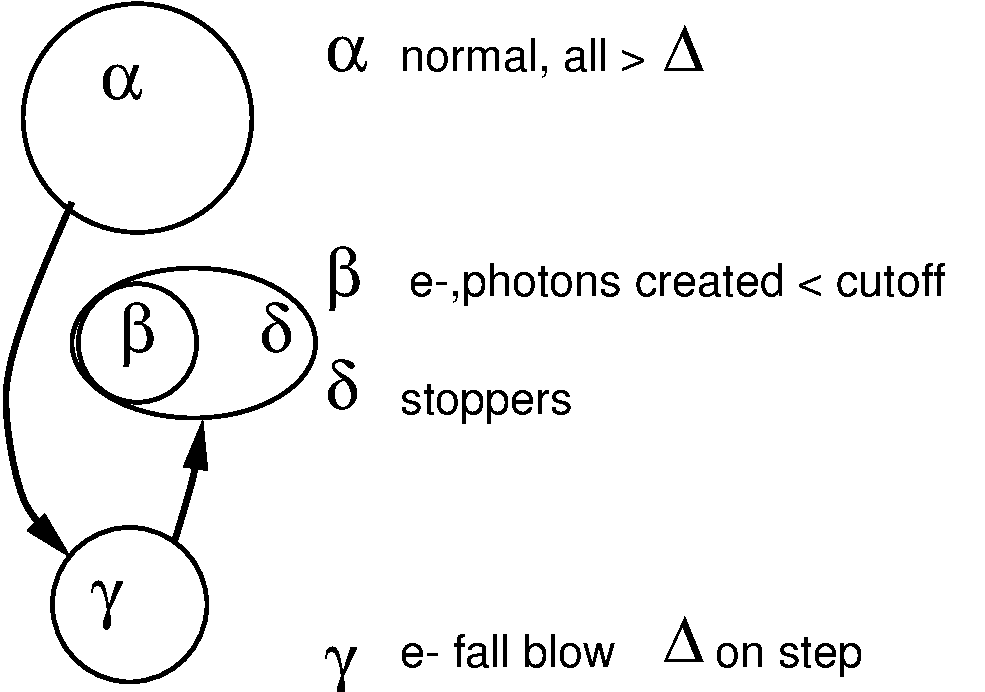
\includegraphics[height=5cm]{figures/sprrz_logic}
\end{center}
\caption[Energy deposition classes in SPRRZnrc]{Modes of energy deposition considered in SPRRZnrc. $\alpha$ events
are those in which energy is deposited by electrons in a step with the
energy entirely above $\Delta$. $\gamma$ events are those in which the
electron starts a step with its energy greater than $\Delta$ and ends with
an energy below $\Delta$. The $\delta$ events are all those events in which
an electron or photon are being terminated because they are below the
cutoffs AE or AP.  This includes a subset of $\beta$ events formed by
electrons and photons which are created with their energy initially below
AE or AP.}
\label{fig_spr_logic}
\end{figure}

The dose delivered by the $\alpha$ events in figure~\ref{fig_spr_logic}
is simple to analyze. In the numerator we just sum the actual energy
deposition. In the denominator we sum the energy deposition times
the ratio of restricted stopping powers at the mid-point energy of the
step, i.e.
\eqn{EDEP \frac{\rspE{Emid}{g}}{\rspE{Emid}{m}}}
This gives how much energy would be deposited in medium $g$ instead of
medium $m$.

The $\beta$ events are not scored at all, except in an evaluation of the
total dose. These events correspond to electrons or photons being created
in the cavity region below the respective transport cut-offs. It is
arguable how to deal with these events, but in traditional calculations
starting from electron spectra they were either ignored or lumped in with
the stoppers.  This issue has been discussed in Borg et al, and there is no
clear solution at this time\cite{Bo99a}.  However, the fraction of the dose contributed
in the cavity region from these events is output by SPRRZnrc and found to
be very small for electron beams or for photon beams at \Co~ energies and
higher. This fact makes the problem academic in most situations.  The
problem becomes serious for low-energy photon beams, but here the
application of Spencer-Attix cavity theory is also suspect\cite{Bo99a}.

The $\delta$ or stopper events which are not $\beta$ events,
are scored as part of the track-end term in
eqn(\ref{eq_sa_spr}).  This is done by scoring the natural energy deposition
in the numerator and the same energy deposition multiplied by the ratio of
the unrestricted stopping powers at $\Delta$ (which are equal to the
restricted stopping powers), i.e.:
\eqn{EDEP \frac{\rspt{g}}{\rspt{m}}.}
Note that this does not merely correspond to the energy deposition in the
second medium, because for a stopper, the energy deposition would be the
same in both media (it just deposits all of its energy which is the same in
both cases). The track-end term in eqn(\ref{eq_sa_spr}) is derived to take
into account that the number of stoppers in each medium will differ because
the fluence of particles stopping in each medium will differ and this
number of stoppers is proportional to the stopping power.

The $\gamma$ events, those particles which cross $\Delta$ during their step
are scored by treating the step as having two components.  The component
with energy above $\Delta$ is treated as if it were an $\alpha$ event and
the component of the energy deposited below $\Delta$ is treated as a
$\delta$ event.

\begin{table}[htb]
\begin{center}
\caption{Energy deposition classes and their components}
\begin{tabular}{|cc|}
\hline
IT value & included events \\
\hline
1  & $\alpha + \gamma + (\delta -\beta)$ \\
3  & $\alpha + \gamma$\\
total & $\alpha + \gamma + \delta$ \\
\hline
\end{tabular}
\end{center}
\end{table}
The SPRRZnrc program scores 3 different doses: the total dose;
dose including everything except the
$\beta$ component (stoppers created below $\Delta$)[IT=1]; dose from
$\alpha$ plus $\gamma$ only [IT=3].
The IT=2 and IT=4 components
correspond to the IT=1 and IT=3 components but scored in the $g$ material
as outlined above. The code then outputs: the total dose; the
fraction of the total dose due to included stoppers (IT=1~$-$~IT=3)/total;
and the fraction of the total dose due to excluded stoppers
(total$-$~IT=1)/total.

The IT=2 dose component is the same as the IT=1 dose component except as
modified to represent the dose in the detector medium as described above.
The IT=4 component similarly corresponds to the IT=3 component, i.e. the
dose less the actual stoppers but including the crossers.

The stopping-power ratios are calculated as the IT=1 dose component divided
by the IT=2 dose component (strictly the scored energy depositions divided
by the respective densities are used).  The stopping-power ratio less the
stoppers is calculated by taking IT=3 divided by IT=4.

The code outputs he two different stopping-power ratios to demonstrate that
the inclusion of the stoppers has only a small effect on the overall
stopping-power ratio, which is a good thing since the treatment of the
stoppers is somewhat arbitrary.  However, it should be pointed out that the
$\gamma$ events are not classified as stoppers but in fact they do contain
some element of the stoppers dose since steps are not stopped at $\Delta$,
but rather at some energy slightly less than $\Delta$.



%\clearpage











\subsection{Input/output control}
\index{SPRRZnrc!I/O control}

I/O control input is delimited between \verb+:start I/O control:+\\
and \verb+:stop I/O control:+.  Most I/O control input
for SPRRZnrc is common to all user codes and is described in
section~\ref{common_I_O_control}\lpage{common_I_O_control}.  However,
the {\tt SPR OUTPUT} control is unique to SPRRZnrc and you input it
as follows:
\begin{verbatim}
  SPR OUTPUT
        = regions         (0)  Specify stopping power ratio output by
                               regions (no .plotdat file will be generated)
        = slabs/cylinders (1)  Specify stopping power ratio output by slabs
                               & cylinders (.plotdat file is generated)
***************************************************************************

  IF SPR OUTPUT= regions

  SPR START REGION   (M)  region numbers in which to start scoring stopping
                           power ratios

  SPR STOP REGION    (M)  region numbers in which to stop scoring stopping
                           power ratios

***************************************************************************

  IF SPR OUTPUT= slabs/cylinders

  SPR IN CYLINDER IX  (M)  Cylinder numbers for which to output
                           stopping power ratios (= 0 for no output)

  SPR IN SLAB IZ      (M)  planar slab numbers for which to output
                           stopping power ratios (= 0 for no output)

**************************************************************************
\end{verbatim}
\index{.plotdat!SPRRZnrc}

\subsubsection{{\tt SPR OUTPUT} options}
\index{SPRRZnrc!SPR OUTPUT}

\index{range rejection!SPRRZnrc}
{\tt SPR OUTPUT} is used to determine how stopping power ratios are
output.  If electron range rejection is off, then stopping power ratios
in all regions are output to the {\tt .egslst} file.  If electron
range rejection is on, then stopping power ratios are zeroed in the
{\tt .egslst} file except in regions specified using
{\tt SPR START REGION} and {\tt SPR STOP REGION} (if
{\tt SPR OUTPUT= regions}) or in slabs/cylinders specified using
{\tt SPR IN CYLINDER IX} and {\tt SPR IN SLAB IZ} (if
{\tt SPR OUTPUT= slabs/cylinders}).  In addition, electron range rejection
is automatically turned off in the regions/slabs/cylinders you have selected
for output so that the stopping power ratios will be meaningful.  If you
are using the {\tt SPR OUTPUT= slabs/cylinders} option, then you will also
get a {\tt inputfile\_dd.plotdat} file which contains the stopping power ratios (and
doses) in the selected slabs and a {\tt inputfile\_rad.plotdat} file
containing stopping power ratios (and doses) in the selected cylinders.
This files are in a format that can be plotted
with {\tt xmgrace} or other plotting program.
\index{.plotdat!SPRRZnrc}

\subsection{Monte Carlo control}
\index{SPRRZnrc!Monte Carlo control}

Monte Carlo control input is delimited between
\verb+:start Monte Carlo inputs:+\\
and \verb+:stop Monte Carlo inputs:+. In addition to the Monte Carlo inputs
common to all user codes (see section~\ref{MC_inputs}\lpage{MC_inputs}),
SPRRZnrc has the following Monte Carlo input:
\begin{verbatim}
  PHOTON REGENERATION         (C)  yes => primary photons are regenerated
                                          after they interact and scattered
                                          photons are thrown away.
                                   no (default) => full calculation

\end{verbatim}
\index{photon regeneration!SPRRZnrc}

\subsubsection{{\tt PHOTON REGENERATION} option}
\index{SPRRZnrc!photon regeneration}
\label{photregsect}

The photon regeneration option is used to calculate the stopping power ratios
for electrons resulting from an unattenuated and unscattered photon beam.
If {\tt PHOTON REGENERATION= yes}, then, prior to a pair production,
compton, photoelectric or Rayleigh event, the properties of the photon about
to interact are saved.  After the interaction, any scattered photons or
photons resulting from relaxation process are discarded and (once all
secondary electrons have been transported) transport reverts to the duplicate
photon that was saved just before the interaction.  In addition, photons
resulting from bremsstrahlung events and positron annihilation events are
eliminated on the spot.
%, and positrons resulting from pair events are
%converted to electrons.
%\note{Why are positrons made into electrons in photon regeneration?}
%\note{Same occurs in general? WHY?????}

This option is to be used when calculating stopping-power ratios for use
in air kerma cavity ion chamber standards since the basic theory makes this
assumption. This makes the calculated stopping-power ratio independent of
the details of the geometry as long as there is full buildup.  This is
discussed in detail by Borg et al\cite{Bo99a}.  This option should not be
used when calculating stopping-power ratios in a phantom since in that case
you want the effects of scatter and attenuation to be taken into effect.


%\renewcommand{\rightmark}{{CAVRZnrc}}
%%%%%%%%%%%%%%%%%%%%%%%%%%%%%%%%%%%%%%%%%%%%%%%%%%%%%%%%%%%%%%%%%%%%%%%%%%%
\section{CAVRZnrc}
%%%%%%%%%%%%%%%%%%%%%%%%%%%%%%%%%%%%%%%%%%%%%%%%%%%%%%%%%%%%%%%%%%%%%%%%%%%
\renewcommand{\leftmark}{{CAVRZnrc}}
\index{CAVRZnrc}

\subsection{Introduction}

CAVRZnrc calculates various factors of interest when using cavity ion
chambers such as $A_{att}$ and $A_{scat}$ and $A_{wall}$.
It has been described in detail in various
publications\cite{Bi85,Ro85a,RB90a,Bi90a} and shown to produce results in
good agreement with standard theory\cite{Bo99a}.

\subsection{Cavity inputs}
\index{CAVRZnrc!cavity inputs}

CAVRZnrc requires an extra set of
inputs defining the cavity region.  These inputs must appear between the
delimiters {\tt :start cavity inputs:} and {\tt :stop cavity inputs:}.

If the user has input the radial geometry using
{\tt METHOD OF INPUT= individual} or {\tt METHOD OF INPUT= groups}
(see section~\ref{geomsect}\lpage{geomsect}), then the following inputs must
appear between the cavity input delimiters:
\begin{verbatim}
   NUMBER OF CAVITY REGIONS (I)   number of geometrical zoneS
                                  comprising the cavity.

   REGION NUMBERS OF THE CAVITY  (M)
                                  the array of these zones
                                  (the cavity region numbers)
\end{verbatim}
Thus, the user defines the cavity in terms of region numbers within the
geometry.

Alternatively, CAVRZnrc offers another method for entering the geometry
in which the geometry is
automatically defined based on cavity information specified by the user.
In this case, only {\tt METHOD OF INPUT= cavity information} needs to be
entered between the {\tt :start geometrical inputs:} and
{\tt :stop geometrical inputs:} delimiters.  Then, between the
cavity input delimiters, the following inputs must be supplied:

\begin{verbatim}

   WALL THICKNESS      (R)   thickness of the chamber walls (cms)
                             (defaults to 0.273)

   CAVITY RADIUS       (R)   outer radius of the cavity (cms)

   CAVITY LENGTH       (R)   length of the cavity (cms) (defaults to 0.2)

   ELECTRODE RADIUS    (R)   radius of the electrode (defaults to 0.)

   WALL MATERIAL       (C)   wall material

   only if   ELECTRODE RADIUS > 0.0
   ELECTRODE MATERIAL  (C)   electrode material
\end{verbatim}
CAVRZnrc creates a simple 3-cylinder
({\tt RCYL(1)=ELECTRODE RADIUS, RCYL(2)=\\CAVITY RADIUS, RCYL(3)=
CAVITY RADIUS + WALL THICKNESS}), 3-slab ({\tt ZPLANE(1)=0,\\
ZPLANE(2)=WALL THICKNESS, ZPLANE(3)=WALL THICKNESS + CAVITY LENGTH,\\
ZPLANE(4)=2*WALL THICKNESS + CAVITY LENGTH}) geometry based on these
inputs.  The material in the cavity is assumed to be AIR.  This option was
useful for early calculations but is not adequate for chambers in which we
want to include much detail.

\subsection{Input/output control}
\index{CAVRZnrc!I/O control}
\label{cavrziosect}

As with the other user codes, I/O control inputs must appear within
the delimiters {\tt :start I/O control:} and {\tt :stop I/O control:}.
In addition to I/O controls that are common to all user codes (see
section~\ref{common_I_O_control}\lpage{common_I_O_control}), CAVRZnrc
has the following inputs:
\begin{verbatim}
  STORE INITIAL RANDOM NUMBERS
        = no          (0)  do not store initial random numbers
        = last        (1)  store initial random number for last history
        = all deposited (2)store the initial random number for all
                           that deposit energy in the cavity
        = all         (3)  store all the initial random numbers

  OUTPUT OPTIONS
        = short              (0)  short output -just the cavity summary
                                  and the dose grid.
        = cavity details     (1)  above plus details for each cavity zone
\end{verbatim}
\index{CAVRZnrc!store initial random numbers}
The {\tt STORE INITIAL RANDOM NUMBERS} input has been included here because
CAVRZnrc has one option, {\tt STORE INITIAL RANDOM NUMBERS= all deposited},
that is not included in the other user codes (see
section~\ref{rnssect}\lpage{rnssect}).
With this option, the initial random numbers from only those histories that
end up depositing energy in the cavity region are stored in the
{\tt .egsrns} file.  Then, if the run is resumed with
{\tt IRESUME= start-RNS} (see section~\ref{resumesect}\lpage{resumesect}),
all histories will end up depositing energy in the cavity region.

\index{CAVRZnrc!output options}
If the user chooses {\tt OUTPUT OPTIONS= short}, then dose and correction
factors will only be output for the cavity as a whole.  If
{\tt OUTPUT OPTIONS= cavity details}, then dose and correction factors
will be output for the cavity as a whole and for each region that makes up
the cavity.

\subsection{Monte Carlo control}
\index{CAVRZnrc!Monte Carlo control}

Monte Carlo control input is delimited between
\verb+:start Monte Carlo inputs:+\\
and \verb+:stop Monte Carlo inputs:+.  In addition to Monte Carlo inputs that
are common to all user codes (see
section~\ref{MC_inputs}\lpage{MC_inputs}), CAVRZnrc had the following
Monte Carlo inputs:
\begin{verbatim}
  IFULL
         = dose and stoppers     (0) just calculate total dose
         = Aatt and Ascat        (1) Above plus Aatt, Ascat
         = Ap                    (2) Above plus Ap as well (option
                                     currently disabled)
         = Afl and <s>g/w        (3) Above plus Afl and <s>g,w as well
                                     (option currently disabled)

  STATISTICAL ACCURACY SOUGHT    (R) % statistical accuracy of the total
                                     dose in the peak region that is
                                     sought The program executes until this
                                     accuracy is obtained or the CPU time
                                     runs out.
  PHOTON REGENERATION
         = yes (1) the calculation is performed with regeneration
                           of the parent photon after they have
                           interacted. A typical setting when FANO
                           conditions are examined.
         = no (0)  a normal calculation.
         = no electrons from wall (ifano = 2) secondary electrons from
                           interactions in the cavity wall are immediately
                           eliminated.  Photons are not regenerated.
                           [IFANO]
\end{verbatim}
\index{photon regeneration!CAVRZnrc}

\subsubsection{{\tt IFULL= dose and stoppers} option}
\index{CAVRZnrc!IFULL}
\index{CAVRZnrc!output of dose}
\label{cavrzifullsect1}

If {\tt IFULL= dose and stoppers}, then CAVRZnrc will output the total
dose in the cavity and, if {\tt OUTPUT OPTIONS= cavity details},
in each region making up the cavity to the {\tt .egslst} file.

\subsubsection{{\tt IFULL= Aatt and Ascat} option}
\index{CAVRZnrc!output of $A_{att}$ and $A_{scat}$}
\label{cavrzifullsect2}

The methods used to calculate the various correction factors have been
described in the literature\cite{Bi85,Ro85a,Bi86,RB90a}.
%\note{This section on Awall needs to be completed .}

If {\tt IFULL= Aatt and Ascat}, then CAVRZnrc will output the total dose,
$A_{att}$, $A_{scat}$ and $A_{wall}$ in the cavity and, if {\tt OUTPUT
OPTIONS= cavity details}, in each region of the cavity to the {\tt
.egslst} file. The listing files also include $K_{wall} = 1./A_{wall}$
(etc).

The scatter correction factor, A$_{scat}$, is defined as the ratio of the
total energy deposited in the cavity to the energy deposited by electrons
generated by primary photon interactions~\cite{Bi86}.  In CAVRZnrc,
photons are flagged as secondary if they have been scattered in compton,
or Rayleigh events, generated by bremsstrahlung or positron annihilation
events, generated by atomic relaxations after compton or photoelectric
events, or if their energy is deposited locally because they have
energy $<$ N-shell energy in a photoelectric event.  Once CAVRZnrc has
totalled the energy deposited in the cavity by electrons generated by
primary photons (ECAV$_{prim}$), and the energy deposited in the cavity
by electrons generated by photons flagged as secondary (ECAV$_{sec}$),
A$_{scat}$ is calculated using the equation:

\begin{equation}
A_{scat}=1+\frac{ECAV_{sec}}{ECAV_{prim}}
\end{equation}

\subsubsection{{\tt STATISTICAL ACCURACY SOUGHT}}
\index{CAVRZnrc!statistical accuracy sought}

If you input a value for {\tt STATISTICAL ACCURACY SOUGHT}
other than zero, then CAVRZnrc will stop when the percent uncertainty on the
total dose in the cavity volume (all cavity regions combined) is equal
to {\tt STATISTICAL ACCURACY SOUGHT} provided that
{\tt NUMBER OF HISTORIES} (see section~\ref{histsect}\lpage{histsect})
or {\tt MAX CPU HOURS ALLOWED} (see section~\ref{cpusect} \lpage{cpusect}) have
not been reached first.

\subsubsection{{\tt PHOTON REGENERATION} options}
\index{photon regeneration!CAVRZnrc}

CAVRZnrc offers two photon regeneration options.  If the user selects
{\tt PHOTON REGENERATION= yes}, then photon regeneration is similar to
that in SPRRZnrc (see section~\ref{photregsect}\lpage{photregsect}).
Unlike SPRRZnrc, where it is required for proper
stopping power ratio calculations as used in primary
air-kerma standards, the purpose of this option in CAVRZnrc is
mainly for theoretical benchmark calculations ({\em e.g} testing
for artefacts under Fano conditions). An additional use
could be for an independent verification of $A_{wall}$: one
runs simulations with {\tt PHOTON REGENERATION= ON} and {\tt PHOTON
REGENERATION= OFF}, the
ratio of the two doses is per definition $A_{wall}$. This is
however not very efficient and a better way to accomplish
this task is to use the cross section enhancement or
photon splitting options described below.

The second regeneration option in CAVRZnrc is {\tt PHOTON REGENERATION= no
electrons from wall}.  With this option, charged particles resulting from
pair production, compton and photoelectric events are eliminated provided
that the interaction did not take place inside the cavity.
This is a hack that has been used to study
the dose fraction from photon interactions in the cavity.

\subsection{CAVRZnrc variance reduction techniques}

\subsubsection{Photon cross section enhancement}
\label{cavrz_cse}
\index{cross section enhancement!CAVRZnrc}
\index{CAVRZnrc!cross section enhancement}

The cross section enhancement technique in CAVRZnrc is
similar to the one implemented in DOSRZnrc
(see section \ref{dosrz_cse} page~\pageref{dosrz_cse}) but
in CAVRZnrc it is applied globally in the entire geometry and the value of
$C_e$ is input directly (as opposed to C as input in the DOSRZnrc case).
Cross section enhancement in CAVRZnrc can be turned on by
including the following line in the input file:
\begin{verbatim}

  CS ENHANCEMENT FACTOR=  some real number [cs_enhance]

\end{verbatim}
If the input is missing or less than unity, there will be
no effect.  But if the enhancement factor is set to greater than unity, the
effect is dramatic: all other user input concerning photon forcing,
splitting, exponential transform, etc., is ignored. In addition,
the calculation result \underline{always} corresponds
to the {\tt IFULL= Aatt and Ascat} option, no matter what the
user requested (but only $A_{wall}$ is calculated,
not the individual $A_{scat}$ and $A_{att}$, see
section \ref{cavrzifullsect2}). In addition, all scoring
is done using proper history-by-history statistics using
the common block {\tt score1}.  The drawback is that dose
and $A_{wall}$ are calculated for the whole cavity and
not on a region-by-region basis as under normal
CAVRZnrc operation.

The following text gives a brief description of the differences
to the DOSRZnrc implementation: The motivation behind the
implementation of cross section enhancement in CAVRZnrc was the desire to
have an independent calculation technique for $A_{wall}$ that is
not too inefficient compared to the unweighting technique. Indeed,
$A_{wall}$ can be calculated by running two separate CAVRZnrc
simulations, one with normal transport  and one with attenuation
and scatter removed via the {\tt photon regeneration= on} option. The ratio of the
cavity dose from the former to the dose from the latter calculation is by
definition $A_{wall}$. Because both calculations
are uncorrelated, their uncertainties add in quadrature and so, the uncertainty
on $A_{wall}$ is larger than the individual dose uncertainties.
The purpose of the cross section enhancement implementation in
CAVRZnrc is to make the two necessary dose calculations at once
and thus reduce the uncertainty of $A_{wall}$ because of the strong
correlation between the ``normal'' dose and the dose with
attenuation and scatter removed. To accomplish this task,
scattered photons are killed as in DOSRZnrc with probability
$1/C_e$. If they survive, they are marked as scattered by setting
their {\tt latch} variable to 3. Unlike in DOSRZnrc, the unscattered
portion of primary photons is always kept on the stack and transported.
However, these non-scattered fractions of primary photons are marked
as attenuated primary photons ({\tt latch=2}) with probability
$1-1/C_e$ and therefore their descendents only contribute to the
dose with attenuation and scatter removed. In addition, scatter,
bremsstrahlung and annihilation from {\tt latch=2} particles are
immediately removed from the stack. It is then clear that
{\tt latch=0,2} electrons contribute to the dose with
attenuation and scatter removed, {\tt latch=0,3} electrons to
the normal dose.

\subsubsection{Photon splitting}
\index{photon splitting!CAVRZnrc}
\index{CAVRZnrc!photon splitting}
\label{cavrzsplitsect}

An additional variance reduction scheme offered in CAVRZnrc
is the photon splitting technique.
Input that turns on photon splitting must appear
between the {\tt :start variance reduction:}
and {\tt :stop variance reduction:} delimiters and is:

\begin{verbatim}

 PHOTON SPLITTING=    (I)    Number of times to split a photon
                             If missing or < 2  => normal transport
                             If >= 2 (allowed only for ifull= dose and
                             stoppers or = Aatt and Ascat), the macro
                             $SELECT-PHOTON-MFP essentially replaces the
                             entire PHOTON routine.
                             [n_split]

\end{verbatim}

This technique is borrowed from Ref. \cite{KF99} where it was shown
to increase the efficiency of external photon beam calculations for
radiotherapy by up to a factor of 5. The increase in CAVRZnrc is
not so dramatic, nevertheless an increase in the efficiency
of cavity dose calculations of up to a factor of 3 compared to using photon
forcing has been observed.

This option is only available with {\tt IFULL= dose and stoppers or =Aatt and Ascat}.
It is also possible to use the {\tt ifano} option (only
if {\tt IFULL=0}). Note that with photon splitting
on, all scoring
is done using proper history-by-history statistics using
the common block {\tt score1}.  The drawback is that dose
(and $A_{wall}$ if requested) are calculated for the whole scoring cavity and
not on a region-by-region basis as under normal CAVRZnrc operation.

The algorithm works as follows:
each photon that is to be transported is split into
{\tt n\_split} photons with weights $w_0/${\tt n\_split}
($w_0$ is the original photon weight). The number of
mean-free-paths $\lambda_i$ to the next interaction of the $i$'th
such photon is sampled from
\begin{equation}
\lambda_i = -\ln \left[1 - {\xi + i - 1 \over {\tt n\_split} } \right]
\end{equation}
where $i$ runs from 1 to {\tt n\_split} and where $\xi$ is a random
number. This forces a uniform distribution of interaction sites.
In addition we have $\lambda_{i+1} > \lambda_i$ and therefore
only transport from $\lambda_i$ to $\lambda_{i+1}$ is needed to
get to the interaction site of the $i+1$'st photon from the
interaction site of the $i$'th photon. When one of the split-photons
interacts, all resulting scattered photons are killed with probability
1/{\tt n\_split} and marked as scattered if they survive
({\tt latch=3}). If {\tt IFULL= Aatt and Ascat} or {\tt photon
regeneration= on}, the original photon is
re-created at each interaction site with probability
1/{\tt n\_split} and marked as a regenerated photon ({\tt latch=2}).
As for the cross section enhancement technique, {\tt latch=0,3} particles
contribute to the normal dose, {\tt latch=0,2} particles to the dose
with attenuation and scatter removed. The ratio of the two is
$A_{wall}$ and so, photon splitting is a third independent
technique for calculating this quantity.

A rule of thumb for good efficiency is to use
\eqn{n\_split \ge \frac{N_o}{1. - e^{-\lambda}} }
where $\lambda$ is approximately the number of photon mean free paths in the
geometry of interest and $N_o \ge 5$. For $^{60}$Co, $\lambda$ is about
0.06 for 1 g/cm$^2$ of graphite and so $n\_split$ should be $\ge 80$.

%%%%%%%%%%%%%%%%%%%%%%%%%%%%%%%%%%%%%%%%%%%%%%%%%%%%%%%%%%%%%%%%%%%%%%%%%%%%%
\section{Spherical user codes}
%%%%%%%%%%%%%%%%%%%%%%%%%%%%%%%%%%%%%%%%%%%%%%%%%%%%%%%%%%%%%%%%%%%%%%%%%%%%%

\subsection{Introduction}

Since 2003, the EGSnrc distribution includes a pair of spherical
geometry user codes.
CAVSPHnrc is the spherical analogue of CAVRZnrc, designed for ion chamber
calculations, and has been used extensively for this purpose (see, \eg,
references\cite{Bi90b,RT99}). The other code, EDKnrc, was derived from
SCASPH, an EGS4 user code for the calculation of mono-energetic energy
deposition kernels\cite{Ma88}. EDKnrc has been extended to allow the use
of both monoenergetic and polyenergetic sources.

Both user codes share most of the common features of the RZ user codes
excluding geometry and source types. We will describe these two in the
following subsections and the user is refered to section \ref{Common}
for information on the common input blocks of these codes.

\subsection{Geometry and Material Inputs}

\subsubsection{Geometrical input: spheres and cones}

The geometrical regions subtended by concentric spheres and cones
originating at the common center of the spheres are shown in figure
\ref{fig_spherical}. NR represents the number of spheres and NC the
number of cones. In what follows we explain the input specification of
the geometry.


\begin{figure}[hbt]
\htmlimage{scale=1.2}{}
\begin{center}
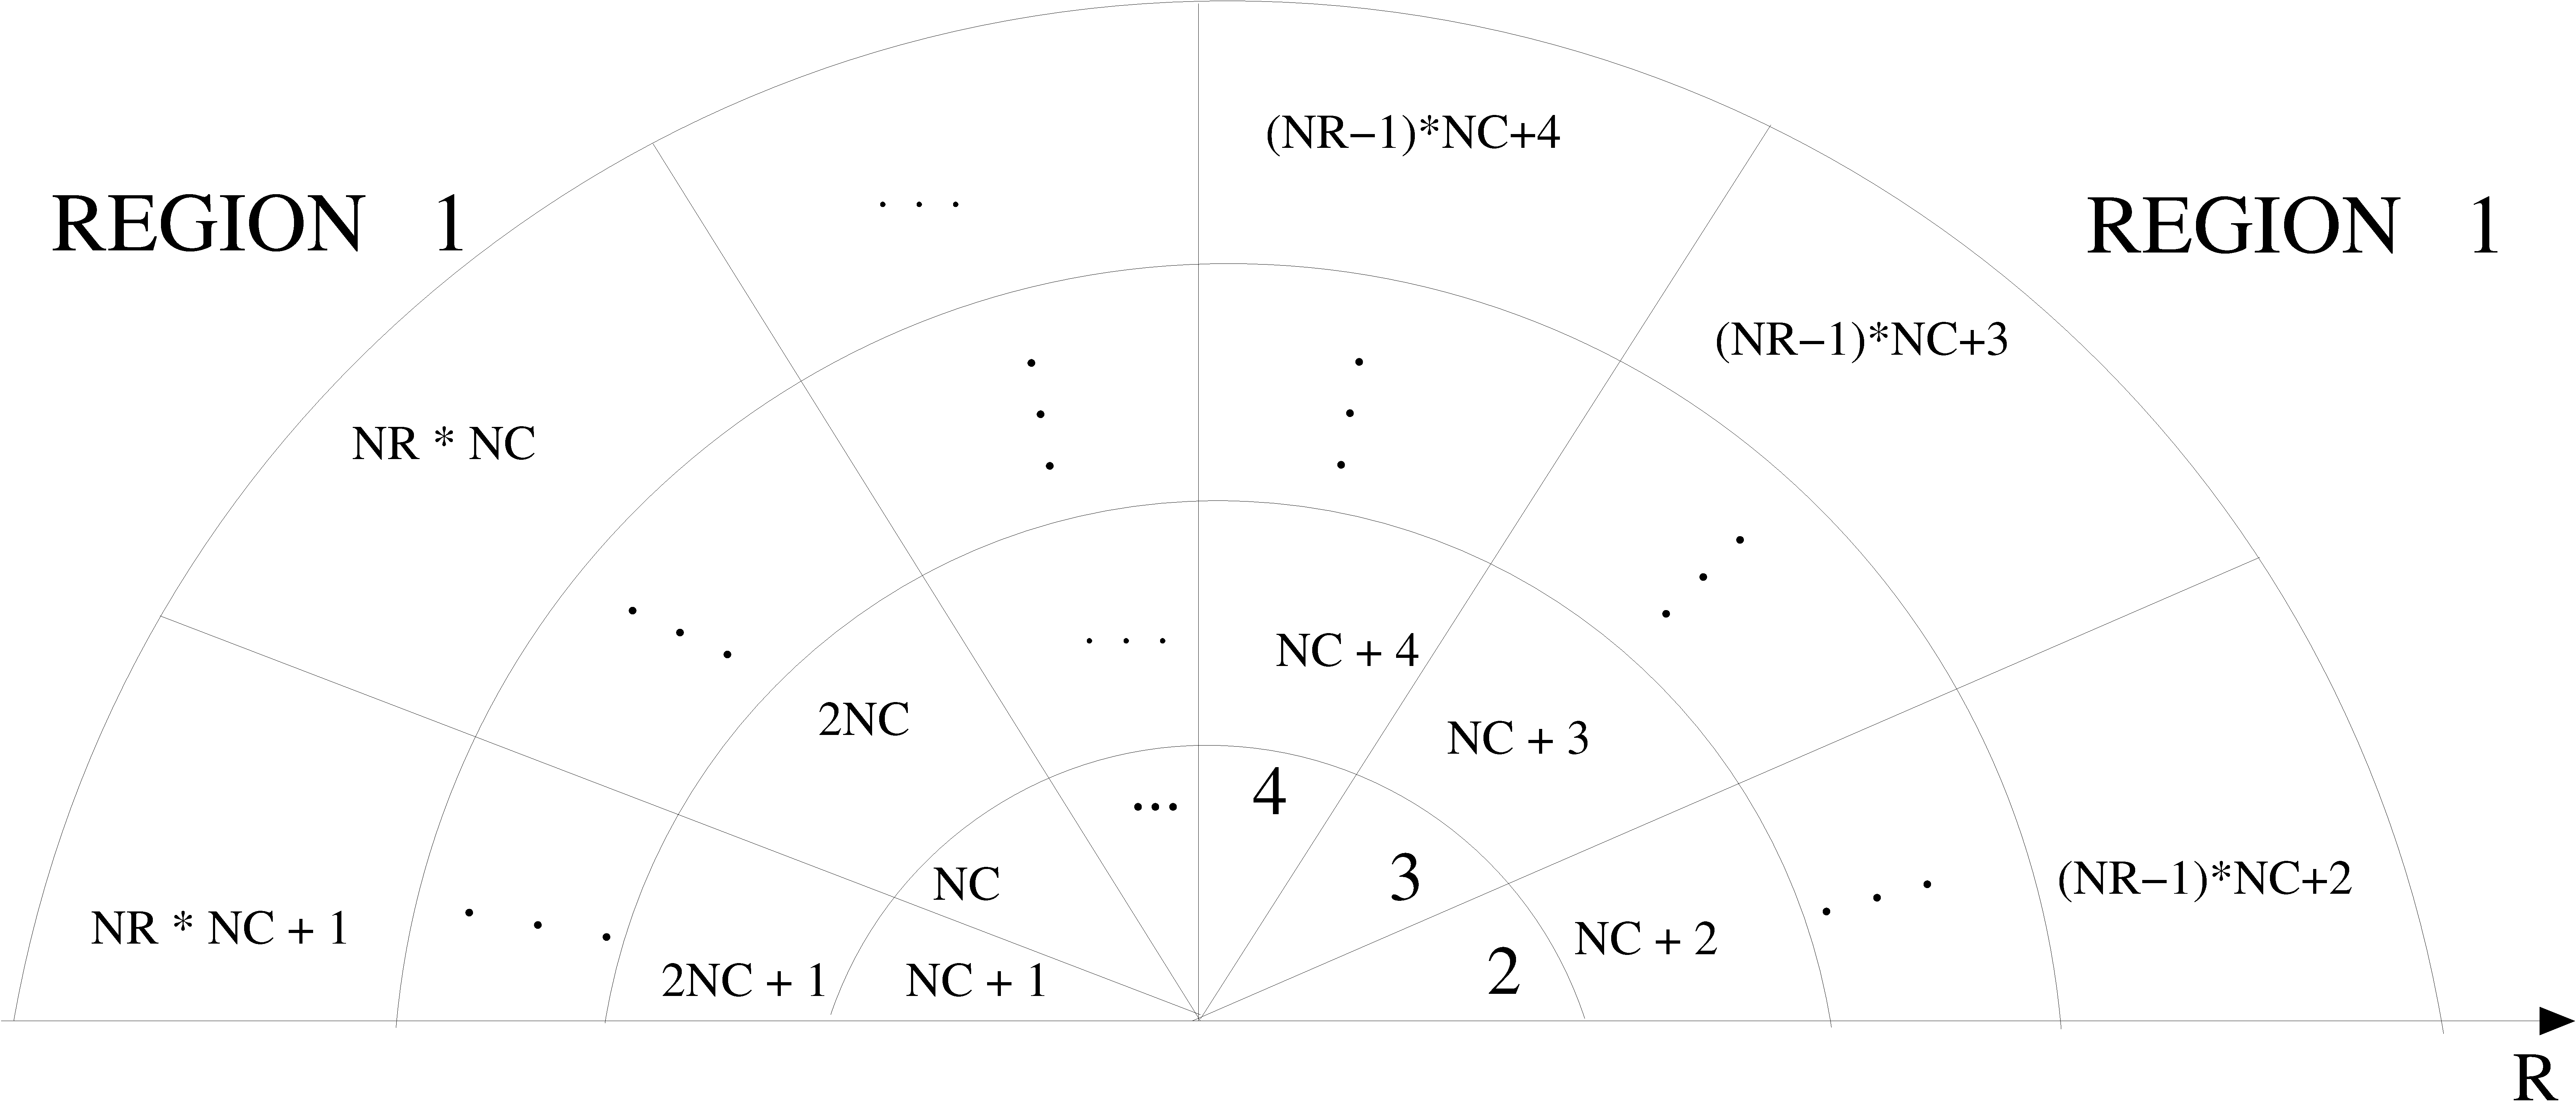
\includegraphics[height=5cm]{figures/spherical}
\end{center}
\caption[Spherical geometry]{Region numbering scheme for the spherical
user codes.  Region number 1 is always outside the geometry. The first
region (2) is defined by the innermost sphere and the cone with the
smallest opening angle. {\tt NR} is the number of radial zones = \# radii
and {\tt NC} = number of cones (0 for purely spherical geometry). }
\label{fig_spherical}
\end{figure}

As in the RZ codes, the geometry inputs are delimited by the strings
{\tt :start geometrical inputs:} and {\tt:stop geometrical inputs:}. The
meaning of the inputs depends on the entries for {\tt NUMBER OF CONES}  and
{\tt NUMBER OF SPHERES}. If a single value is input, then the user is
expected to input the individual corresponding radii or angles. If multiple
values are given for {\tt NUMBER OF CONES}  and/or {\tt NUMBER OF SPHERES},
the user is expected to put in groups of equal angles and/or radii.
If, for instance, several
entries are made for the number of angles, \ie, {\tt NANG1, NANG2, ...}, it
is assumed that the first {\tt NANG1} cones will have the same opening angle
and so on. For spheres, if the user omits the number of radii, it is
assumed that individual entries will be made (after all,
these are user-codes for spherical problems).

\begin{verbatim}
 NUMBER OF CONES= [NANG(1)[,NANG(2),...,NANG(K)]]
                  # If omitted or ZERO, pure spherical geometry assumed
 NUMBER OF SPHERES= [NRAD(1)[,NRAD(2),...NRAD(J)]]
                  # no needed for individual input
\end{verbatim}

Once the user has defined the number of spheres and cones in the problem, the
actual values for the radii and angles must be entered, using the keywords
outlined below:

\begin{verbatim}
RADII= RAD(1), RAD(2), ...RAD(j)
                  #radii of spheres defining the geometry
                  #For group input there must be as many entries
                  #as for the NUMBER OF SPHERES, i.e. :
                  #         J = j
                  #For individual input, NRAD(1) must be equal
                  #to the number of entries, i.e.:
                  #        NRAD(1) = j
                  #unless NUMBER OF SPHERES is omitted, in which case
                  #indiviual input is automatically assumed.
ANGLES= ANG(1), ANG(2),...,ANG(3)
                  #The same rules apply for angles as for radii apply.
\end{verbatim}

One can also enter a group of regions to be considered as the cavity
of a spherical ion chamber and the total dose in these regions will
be computed. For CAVSPHnrc, quantities such as
$K_{att}$ and $K_{scat}$ and $K_{wall}$ are also calculated for the
whole cavity. The specification for the cavity inputs is:
\begin{verbatim}
CAVITY ZONES= [REG1[, REG2...,REGn]] #geometrical zones defined as the
                                     #cavity (real numbers)
\end{verbatim}

\subsubsection{Material input.}

These codes have a simple structure for entering the material input. First
the user must provide a list of media in the problem where the first
medium is taken as default, \ie, every region is considered to have this
medium. Then, medium numbers for all regions where the medium is not
medium 1 must be specified.


\begin{verbatim}
 MEDIA= MEDIUM1, MEDIUM2,..., MEDIUMn

 MEDNUM=        MEDIUM2, MEDIUM2, MEDIUM3,..., MEDIUMn
 START REGION=  START1,  START2,  START3,...,  STARTn
 STOP REGION=   STOP1 ,  STOP2,   STOP3, ...,  STOPn

\end{verbatim}

\subsection{CAVSPHnrc}
The NRC user code CAVSPHnrc (spherical geometry) like CAVRZnrc
(cylindrical geometry) calculates various factors of interest when using
ion chambers such as $K_{att}$, $K_{scat}$, $K_{wall}$ and the dose to the
cavity region per unit incident fluence.

The input file for this user code is very similar to the one for
CAVRZnrc. Only two input blocks are different, the geometry input block
and the input block for the sources. The geometry input was described
previously and the input for the sources differ from CAVRZnrc, in that
only four source types are available: a parallel beam from any angle
(source 0), a point source from any angle (source 1), a parallel beam
from any angle with radial distribution (source 10), a point source from
any angle with radial distribution (source 11).
and a point source from any angle. The source input block is defined by
the delimeters {\tt :start source inputs:} and {\tt :stop source inputs:}
and the same inputs are needed as in CAVRZnrc (see
section~\ref{source_inputs} on page~\pageref{source_inputs}).  In
particular, one must define:

\begin{verbatim}
  INCIDENT PARTICLE= electron   (-1)  electrons
                     photon     (0)   photons
                     positron   (1)   positrons

  SOURCE NUMBER                 (I)   number of the source
                                      [ISOURC]
  SOURCE OPTIONS                (M)   four or five real numbers as specified
                                      below

------------------------------------------------------------------------------

 SOURCE 0/10:  FOR PARALLEL BEAM FROM ANY ANGLE (10-->WITH RAD. DISTN)
              RBEAM,UINC,VINC,WINC
               RBEAM   RADIUS OF THE BEAM AT THE FRONT OF THE TARGET IN CM
                               DEFAULTS TO MAX RADIUS
               UINC    INCIDENT X-AXIS DIRECTION COSINE
               VINC    INCIDENT Y-AXIS DIRECTION COSINE
               WINC    INCIDENT Z-AXIS DIRECTION COSINE
                       NOTE: (UINC,VINC,WINC) GET AUTOMATICALLY NORMALIZED
                             DEFAULTS TO (0.0,0.0,1.0)
------------------------------------------------------------------------------

 SOURCE 1/11:  FOR POINT SOURCE INCIDENT FROM ANY ANGLE (11-->WITH RAD. DISTN)
             DISTR,RBEAM,UINC,VINC,WINC
               DISTR   DISTANCE OF THE SOURCE FROM THE MIDDLE OF THE TARGET
                       IN CM (DEFAULTS TO 100.)
               RBEAM   RADIUS OF THE BEAM AT THE FRONT OF THE TARGET IN CM
                               DEFAULTS TO MAX RADIUS
               UINC    INCIDENT X-AXIS DIRECTION COSINE
               VINC    INCIDENT Y-AXIS DIRECTION COSINE
               WINC    INCIDENT Z-AXIS DIRECTION COSINE
                       NOTE: (UINC,VINC,WINC) GET AUTOMATICALLY NORMALIZED
                             DEFAULTS TO (0.0,0.0,1.0)
------------------------------------------------------------------------------

 SOURCE 10 OR 11:
       SPECIFY MODE:
               MODE = local (0)     IF RADIAL DISTRIBUTION IS TO BE INPUT
                                    LOCALLY WHETHER THROUGH THE KEYBOARD
                                    (INTERACTIVE USE) OR THROUGH THE
                                    .INP FILE (DEFAULT)
                    = external (1)  IF THE DISTRIBUTION IS TO BE INPUT
                                    VIA AN EXTERNAL FILE
       IF MODE=local SPECIFY:

           RDISTF(I)= TOP OF RADIAL BIN I FOR I=1,NBIN
           RPDF(I)= PROBABILITY OF INITIAL PARTICLE BEING IN BIN I FOR
                    I=1,NBIN.

                      PROBABILITIES DO NOT NEED TO BE NORMALIZED
                      BUT SHOULD BE IN UNITS CM**-2

       IF MODE=external SPECIFY:

           RDIST FILNAME = FILENAME(WITH EXT) CONTAINING THE ABOVE INFORMATION


       SPECIFY:
           DISTRIBUTION DATA = NONE => NO DISTRIBUTION DATA IN OUTPUT SUMMARY
                             = OUTPUT SUMMARY => INCLUDE DISTRIBUTION
                               DATA IN OUTPUT SUMMARY
\end{verbatim}

\subsection{EDKnrc}

The NRC user code EDKnrc can be used to calculate Energy Deposition Kernels
for photons or electrons (monoenergetic or polyenergtic) forced to interact
at the centre of a spherical
geometry\cite{Ma05}.  The code can output energy deposition kernels (EDK),
dose distributions in the phantom or the dose to regions defined as the
cavity of a spherical ion chamber.  Voxels are defined by the intersection
of a spherical shell with two cones. See figure \ref{fig_spherical}
for more details.

Although the geometry inputs for this user code are similar to CAVSPHnrc,
there are some major differences in other inputs. The input block for I/O
control, defined by the delimeters {\tt :start I/O control:} and
{\tt:stop I/O control:}, is severely abbreviated.  It includes an entry,
{\tt PRINT OUT EDK FILE} that defines whether energy deposition
kernels will be output in the same format as the ones calculated by
Mackie {\it et al.}\cite{Ma88}. The entire input for this block
is shown below:

\begin{verbatim}

:start I/O control:
  IRESUME
       = first    (0) First run for this data set
       = resume   (1) Resume a previous run
       = analyze  (3) Just read in the raw data and do the statistical analysis
       = parallel (5) Combine results from previous parallel runs
  STORE DATA ARRAYS
       = yes             (0) Store data arrays for re-use
       = no              (1) don't store them
  PRINT OUT EDK FILE
       = yes             (0) EDK stored in old format files
       = no              (1) don't produce EDK files in old format
:stop I/O control:
\end{verbatim}


The input block defining Monte Carlo parameters (delimited by
{\tt start}/{\tt stop Monte Carlo inputs:}) is also abbreviated.  Here
one specifies only the number of histories, the initial random number
seeds, and a variable {\tt IFULL}, which specifies the type of calculation,
and an input specifying whether doppler broadening is to be taken into
account during Compton interactions.

\begin{verbatim}

IFULL= cavity calculation        #(0) calculate dose in cavity regions
     = energy deposition kernels #(1) calculate and output EDK's
     = dose calculation          #(2) calculate and output dose
     = dose and edk              #(3) calculate and output EDK's and dose

DOPPLER BROADENING= On
                  = Off

\end{verbatim}

EDKnrc allows for only three possible sources: 1) a photon source algorithm
that forces photons moving along the Z-axis to interact at the origin
(source 0) 2)
an isotropic point source at the origin for any type of
particle (source 1) 3) same as source 0 but with interaction point shifted
to a user-specified position on the Z-axis (source 2).  Source 2
was left for comparison with older EDK calculations, but the user
is strongly discouraged from using it, since it has been shown to produce
numerical artifacts when computing EDK's. For accurate EDK calculations
source 0 should be used.   The inputs specifying the source type, which is
included within the {\tt start}/{\tt stop Source Inputs:} delimiters,
are shown below:

\begin{verbatim}
SOURCE NUMBER= 0 | 1 | 2
#     0 ==>  Photon moving along Z axis forced to interact at origin
#     1 ==>  Point source at origin, isotropically radiating into 4 Pi
#     2 ==>  Same as 0 but interaction point as in old code

# if SOURCE NUMBER= 2
    ZIN      #-> source offset on Z-axis
             #   Option used to emulate old way of calculating EDK
\end{verbatim}

Note that in the case of source 0 or source 2, the {\tt INCIDENT PARTICLE=}
(standard for all user codes when specifying the source) input must be
set to {\tt PHOTON}.

The energy deposited in the geometry can be separated into different
contributions from each photon scattering order (\eg~ primary,
first scatter, second scatter, multiple scatter and radiative). For
electrons, the deposited energy can be split into primary and radiative
contributions. In the standard output file {\tt *.egslst}, only the total
and primary components are written. ONLY if the user selects the option
for creating old format EDK files, all components are stored to a file
following the convention:
\begin{itemize}
\item {\tt edk[EIN].keV}, for monoenergetic sources,
where EIN is the initial energy in keV.
\item {\tt file\_name.keV}, for polyenergetic sources (spectrum),
where {\tt file\_name} is the standard output file name

\end{itemize}

The user also has the choice to
create xmgrace plot files for the {\bf total dose} by using the input block for plot control delimited by
{\tt :start plot control:} and {\tt:stop plot control:}. A description of this input block is
given below:

\begin{verbatim}
   :start plot control:

   PLOTTING
          = Off         (0)   no plots or plot files to be prepared
          = Histogram   (1)   histogram plotting
          = Point       (2)   xy graph


  ONLY IF not PLOTTING= Off

   PLOT RADIAL REGION IX  (M)  radial regions to plot vs angle
                               (= 0 for no plots)

   PLOT CONICAL REGION IC  (M)  angular intervals to plot vs radius
                               (= 0 for no plots)

   :stop plot control:
\end{verbatim}

Plots in radial regions are written to the file {\tt inputfile.angplot}
({\em i.e.} dose versus angle) and plots in conical regions are written
to the file {\tt inputfile.radplot}.

The output capabilities of this user code are very limited but can be
easily extended to print out all components of the energy deposition
kernels.

\typeout{}
\typeout{***Start of Cited References****}
\typeout{}
\renewcommand{\leftmark}{{REFERENCES}}
\renewcommand{\rightmark}{{REFERENCES}}
\section{References}
\vspace*{-1.7cm}
\bibliography{../irs}
%above points to where we find the master reference list
\typeout{}
\typeout{******REMEMBER to create .bbl  and reset twice**********}
\typeout{}
\bibliographystyle{unsrt}


\newpage
\typeout{**********starting index here******************}
\renewcommand{\leftmark}{{Index}}
\renewcommand{\rightmark}{{Index}}
\addcontentsline{toc}{section}{\numberline{}Index}
\setlength{\baselineskip}{0.5cm}


%%%%%%%%%%%%%%%%%%%%%%%%%%%%%%%%%%%%%%%%%%%%%%%%%%%%%%%%%%%%%%%%%%%%%%%%%%%%%%%
%
%  EGSnrc user codes manual
%  Copyright (C) 2021 National Research Council Canada
%
%  This file is part of EGSnrc.
%
%  EGSnrc is free software: you can redistribute it and/or modify it under
%  the terms of the GNU Affero General Public License as published by the
%  Free Software Foundation, either version 3 of the License, or (at your
%  option) any later version.
%
%  EGSnrc is distributed in the hope that it will be useful, but WITHOUT ANY
%  WARRANTY; without even the implied warranty of MERCHANTABILITY or FITNESS
%  FOR A PARTICULAR PURPOSE.  See the GNU Affero General Public License for
%  more details.
%
%  You should have received a copy of the GNU Affero General Public License
%  along with EGSnrc. If not, see <http://www.gnu.org/licenses/>.
%
%%%%%%%%%%%%%%%%%%%%%%%%%%%%%%%%%%%%%%%%%%%%%%%%%%%%%%%%%%%%%%%%%%%%%%%%%%%%%%%
%
%  Authors:         Dave Rogers
%                   Iwan Kawrakow
%                   Jan Seuntjens
%                   Blake Walters
%                   Ernesto Mainegra-Hing
%
%  Contributors:    Frederic Tessier
%
%%%%%%%%%%%%%%%%%%%%%%%%%%%%%%%%%%%%%%%%%%%%%%%%%%%%%%%%%%%%%%%%%%%%%%%%%%%%%%%


\documentclass[12pt,twoside]{article}  %indexm doesn't work with two
					%sides
%\usepackage{supertab}%this didn't work for some reason?
%\usepackage{overcite}			%comment out for html?

\usepackage{moreverb}	%this is used for the boxedverbatim environment
			%used to box the listing files for tutor programs

\setlength{\textwidth}{16.51cm}
%\setlength{\textheight}{23.2cm}
\setlength{\textheight}{23.5cm}
\setlength{\oddsidemargin}{0.0in}
\setlength{\evensidemargin}{0.0in}
\setlength{\topmargin}{-1.5cm}
\setlength{\parindent}{1.5em}
\setlength{\topsep}{0ex}
\setlength{\itemsep}{0ex}

\newcommand{\lpage}[1]{(page~\pageref{#1})}
\newcommand{\Mol}{Moli\`ere}

\newcommand{\Co}{$^{60}$Co}
\newcommand{\parsp}{~\hspace*{1.5em}}
\setlength{\parskip}{0.1in}
\setlength{\baselineskip}{1.0cm}
\newcommand{\head}[1]{\begin{center}\begin{Large}{\bf #1}
                                              \end{Large}\end{center}}
\newcommand{\cen}[1]{\begin{center} #1 \end{center} }
\newcommand{\etal}{{\em et.al.}}
\newcommand{\ie}{{\em i.e.}}
\newcommand{\etc}{{\em etc.}}
\newcommand{\viz}{{\em viz.}}
\newcommand{\eg}{{\em eg.}}
\newcommand{\sprt}[2]{\left(\frac{\overline{L}}{\rho}\right)^{\rm #1}_{\rm #2}}
\newcommand{\eqn}[1]{\begin{equation} #1 \end{equation} }
\newcommand{\rsp}[1]{\left( \frac{L(\Delta)}{\rho} \right)_{#1}}
\newcommand{\PhiT}{\Phi_{\rm T}}
\newcommand{\rspt}[1]{\left( \frac{S(\Delta)}{\rho} \right)_{#1}}
\newcommand{\rspE}[2]{\left( \frac{L({\rm #1})}{\rho} \right)_{#2}}

\newcommand{\note}[1]{\mbox{}\\ \noindent \rule{16cm}{0.5mm} \\
{\em #1} \\ \noindent \rule{16cm}{0.5mm}\\
\typeout{******note: #1 *****}
}

%\newcommand{\indexm}[1]{\index{#1}}
%\typeout{~~~~~~~~~~~~***margin index feature OFF*****************************}
%\typeout{~~~~~~~~~~~~***margin index feature OFF*****************************}
%\typeout{~~~~~~~~~~~~***margin index feature OFF*****************************}
\newcommand{\indexm}[1]{\marginpar{{\sf {\tiny I:#1} }}\index{#1}}
\makeindex


\renewcommand{\refname}{}

%       some commands to get 4 levels in the table of contents and
%       number down to paragraphs
\setcounter{secnumdepth}{4}
\setcounter{tocdepth}{4}
\renewcommand{\thesubsubsection}{\thesubsection.\arabic{subsubsection}}
\renewcommand{\theparagraph}{\thesubsubsection.\roman{paragraph}}
%\renewcommand{\theequation}{\arabic{subsection}.\arabic{subsubsection}.\arabic{equation}}



%\usepackage{html}
\usepackage{graphicx}
%\usepackage{epsf}
%\input{epsf}
\usepackage{longtable}

\usepackage{fancyhdr}
\renewcommand{\footrulewidth}{0.4pt}
\renewcommand{\headrulewidth}{0.4pt}

\lhead[{\sffamily \thepage}]{{\sffamily NRC User Codes for EGSnrc }}
\rhead[{\sffamily NRCC Report PIRS-702}]{{\sffamily ~\thepage}}
%\rfoot[{\sffamily {\rightmark}}]{{\sffamily {\rightmark}}}
\rfoot[]{{\sffamily {\rightmark}}}
% \lfoot[{\sffamily {\leftmark}}]{{\small Last edited $Date: 2013/09/24 18:04:14 $
\lfoot[{\sffamily {\leftmark}}]{{\small Last edited 2011/05/03 15:50:14
}}
\cfoot{}

\usepackage{hyperref}
\hypersetup{colorlinks=true, citecolor=blue, linkcolor=blue, filecolor=blue, urlcolor=blue}
\urlstyle{same}

\usepackage{html}



\begin{latexonly}
\typeout{***Have turned off overfull and underfull messages****}
\tolerance=10000        %suppress Overfull only
\hbadness=10000         %suppress Overfull and Underfull for text (horizontal)
\vbadness=10000         %suppress Overfull and Underfull for vertical "boxes"
\end{latexonly}


\begin{document}

\begin{htmlonly}
For information about the authors and/or institutions involved with this
work, use the links provided in the author list.\\

\begin{rawhtml}
<br><br>
\end{rawhtml}


Postscript versions of the entire paper are available.  You may have to
download the compressed version to disk, uncompress or gunzip them and
then read or print them.\\
\begin{center}
\htmladdnormallink{(uncompressed version 2.4 Mb)}{pirs702.ps}\\
\htmladdnormallink{(gzip version 230 kb)}{pirs702.ps.gz}\\
\htmladdnormallink{(pdf version 440 kb)}{pirs702.pdf}\\
\end{center}
\begin{rawhtml}
<br><br>
\end{rawhtml}

Use the Up button to get back to this page from within the document.
\begin{rawhtml}
<BR> <HR> <P>
\end{rawhtml}
\copyright
Copyright 2021,  National Research Council of Canada
Ottawa
\begin{rawhtml}
<BR> <HR> <P>
\end{rawhtml}
\end{htmlonly}

\pagestyle{empty}

\title{NRC User Codes for EGSnrc}

\begin{center}
{\sffamily \bfseries {\Huge NRC User Codes for EGSnrc}
\vspace{5mm}\\}
\begin{Large}
D.W.O. Rogers, I. Kawrakow, J.P. Seuntjens,  B.R.B. Walters and E.
Mainegra-Hing \\
\end{Large}
Ionizing Radiation Standards,
National Research Council Canada, Ottawa, Canada\\


\vspace{3mm}
{\bfseries
\today}
%January 2010}
\vspace{3mm}\\
\hfill NRCC Report {\sf PIRS-702(revC)} \vspace*{2mm}\\

\begin{figure}[h]
\htmlimage{scale=1.2}{}
\begin{center}
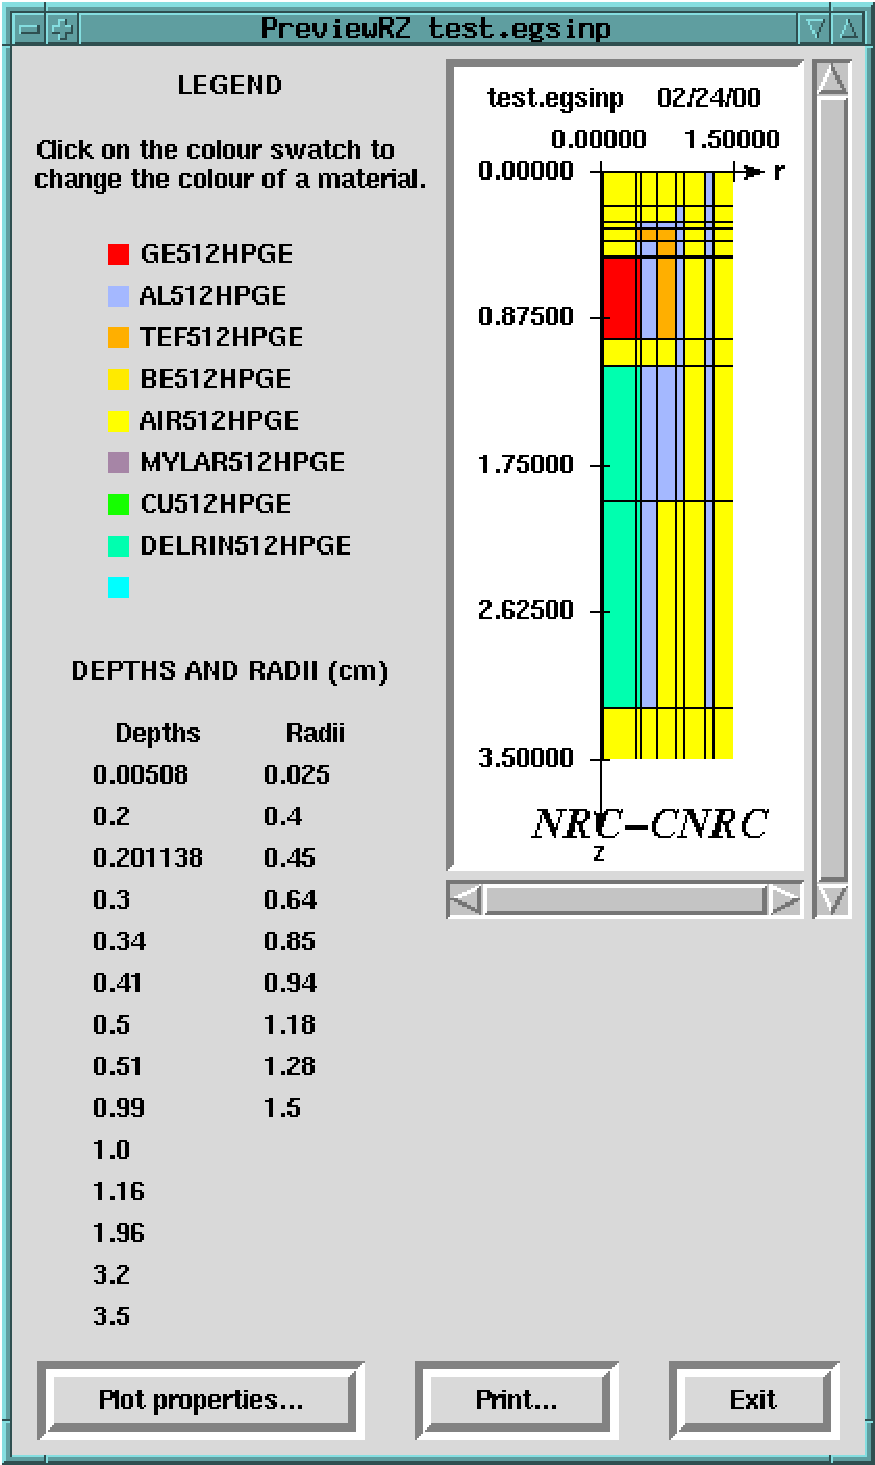
\includegraphics[height=12cm]{figures/PreviewRZ_example}
\\Preview of an RZ geometry in DOSRZnrc.
\end{center}
%\caption{Preview of an RZ geometry in DOSRZnrc.}
%\cen{Get a figure from preview tcl of DOSRZnrc}
\end{figure}

\vfill
\begin{latexonly}
\end{latexonly}

\copyright NRC Canada, 2021
\end{center}
\newpage   %Blank page behind cover
\mbox{}

%\note{This page is intentionally blank to be the back of the front cover.
%Remove this note prior to printing!!!}

\setlength{\baselineskip}{0.5cm}
\newpage

\pagestyle{fancy}
\pagenumbering{arabic}
\setcounter{page}{1}


\begin{abstract}
\label{abstract}
This manual describes the NRC User codes DOSRZnrc, CAVRZnrc, FLURZnrc and
SPRRZnrc which all work with the EGSnrc Code system for Monte Carlo
transport of electrons and photons (see NRC REPORT PIRS--701, ``The EGSnrc
Code System''). There is a graphical user interface available for creating
the inputs to these codes (described separately).

\end{abstract}

%\newpage

\setlength{\baselineskip}{0.1cm}

\tableofcontents

%\newpage
\listoftables
\listoffigures

\setlength{\baselineskip}{0.5cm}

\newpage

\renewcommand{\leftmark}{{INTRODUCTION}}
\section{Introduction}
\subsection{Intent of this report}

Over the years, NRC has developed and distributed a series of user codes
for use with the EGS4 code system for the Monte Carlo simulation of photon
and electron transport.  These have been widely used and their results
compared to experiment in many cases.  However, the codes themselves have
never been properly documented and described. It is the purpose of this
manual to provide a document which describes
both how these codes work and also how a user uses them.  It is not the
purpose of this manual to discuss selection of parameters when using these
codes for a particular application since this is a huge undertaking and is
covered in the already extensive literature on EGS.

Recently, the codes
have been reworked to use the new EGSnrcMP system\cite{Ka03}. This
has increased the flexibility of these codes, including the ability
to run them on both Unix/Linux and Windows systems.

The codes involved in this report are all for
cylindrical RZ and spherical geometries. These are:
\begin{description}

\item[DOSRZnrc] which scores dose in a generalised cylindrical geometry.

\item[FLURZnrc] which scores particle fluence in the same geometry.

\item[CAVRZnrc] which is similar to DOSRZnrc but also scores a variety of
quantities which are of specific interest to dosimetry
calculations for an ion chamber.

\item[SPRRZnrc] which calculates Spencer-Attix spectrum averaged
stopping-power ratios for arbitrary media.

\item[CAVSPHnrc] which is identical to CAVRZnrc but for spherical
geometries.

\item[EDKnrc] which calculates energy deposition kernels for photons
or electrons forced to interact at the centre of a spherical phantom.
It can also calculate dose distributions in the entire phantom or the
dose to specific regions defined as the cavity of a spherical ion chamber.

\end{description}

This manual does not describe the BEAM code for modelling radiotherapy
accelerators, \Co~ units and x-ray systems. BEAM is described
elsewhere\cite{Ro95,Ro98a}. The user codes
described here all have the capability of using either a BEAM generated phase
space file or a full BEAM simulation (compiled as a shared library)
as the source of incident particles.

Also, this manual does not describe the EGS\_Windows system for doing 3D
displays of EGS simulations. EGS\_Windows is described in detail in its own
manual\cite{TR99a}.

\subsection{History}
\index{history}
These codes have a long history at NRC and were first written to work
with EGS3 which was written in Mortran2.  The first germs of these
codes were written by Alex Bielajew who was responsible for coding
CAVRZ as a research tool for work related to ion chamber dosimetry.
This then grew into DOSRZ which strips out some of the special purpose
parts of CAVRZ but adds various more general purpose facilities such as
calculating response functions for detectors. Dave Rogers took these
codes and developed a general purpose fluence scoring code FLURZ and
finally SPRRZ was developed.  Along the way various summer students worked
under Dave Rogers and Alex Bielajew to add features.

One problem was that
all the codes had grown on their own with various bits and pieces being
patched in whenever they were needed for a particular research project.
The system of codes was getting more and more difficult to maintain
and various options failed to work on new systems as they came along
(eg the output listing from FLURZ didn't work on Unix systems
because it was based on a
Digital Vax Fortran extension which was not commonly available on unix
Fortran compilers).  This was overcome in the DOSRZ code by some horrific
coding tricks which made it impossible to change the outputs.  Furthermore the
input files became almost impossible to create since they were just a
large file of numbers where the meaning of each number was dependent on
its position, and often meant different things for the different codes.

To overcome these shortcomings, a major revamping was undertaken in 1998
by Aaron Merovitz, a summer student working for Dave Rogers.  Firstly he
created some general purpose output routines which worked for standard
compilers. Also, as much as possible all graphical output was done through
a single subroutine called {\tt xvgrplot} so that if changes in plotting
output are required. it needs to be changed in only the subroutine.
Next a text based system for input files was written which is much easier
to use than the previously used long string of numbers.  This tool was
then used to create a single routine to read geometry inputs for all the
user codes so that now one can cut and paste the geometry description
from one user code to another. This was extended for source routines and
transport routines so that the input files start to look similar for all
the user codes.  More importantly they are much easier to read and know
exactly what the simulation is about without having the description of
the inputs open on your desk.

In 1999, the codes were upgraded to use the then-new EGSnrc code system.
This was done by Iwan Kawrakow with Jan Seuntjens and Dave Rogers.
In the process many small bugs have been found and fixed.

In 2002, Ernesto Mainegra-Hing developed a very powerful C$++$ graphical
user interface which is based on the Qt(version 3) system\cite{Ma03}.

The final major upgrade has been to make the codes work with the new
EGSnrcMP code system. This has been undertaken by Iwan Kawrakow with
support from Ernesto Mainegra-Hing and Blake Walters.

In the individual descriptions below of the codes we cite various specific
references to papers in which the various aspects of the code have been
described.

As the above history makes clear, these user codes have been developed
by many different people over a long period of time, and the codes
have all benefited by extensive feedback and bug patches from the user
community. In particular, we wish to recognise the contribution of Alex
Bielajew to the development of these codes over a long period of time
while he was at NRC.

\renewcommand{\leftmark}{{COMMON FEATURES}}
\section[Common Features]{Common Features of All Codes and Associated Inputs}
\label{Common}
\subsection{Subroutines in the RZ codes}

\index{subroutines}
As pointed out before, all NRC RZ-codes work within the same RZ
geometry, and their \verb+HOWFAR+ and \verb+HOWNEAR+ routines are
exactly the same. Most of the other common subroutines and macros
have been split off as much as possible (but not completely)
from the user code file. They include:

\begin{itemize}
\item{random number generators (\verb+ranmar.macros+,
\verb+ranmar.mortran+,\\
\verb+ranlux.macros+, \verb+ranlux.mortran+)}
\index{random number generators}

\item{machine specific macros / routines
(\verb+machine.mortran+)}
\index{machine.mortran}

\item{EGSnrc specific macros and routines
(\verb+egsnrc.mortran+, \verb+egsnrc.macros+)}

\item{RZ geometrical subroutines
(\verb+geomrz.mortran+)}
\index{geomrz.mortran}

\item{input parser routines
(\verb+get_inputs.mortran+, {\tt transportp.macros})}
\index{get\_inputs.mortran}
\index{transportp.macros}

\item{Sources and energy sampling routines available for the RZ codes
(\verb+srcrz.mortran+, \verb+ensrc.mortran+, {\tt srcrz.macros},
{\tt phsp\_macros.mortran})}
\index{srcrz.mortran}
\index{srcrz.macros}
\index{ensrc.mortran}
\index{phsp\_macros.mortran}

\item{{\tt IWATCH} output routine
(\verb+nrcaux.mortran+)}
\index{nrcaux.mortran}

\item{Routine to output RZ grid to {\tt .egslst} file ({\tt grids.mortran})}
\index{grids.mortran}

\item{Routines for initializing data I/O, opening output files, etc
({\tt egs\_utilities.mortran})}
\index{egs\_utilities.mortran}

\item{Routines for built-in parallel processing functionality
({\tt egs\_parallel.mortran})}
\index{egs\_parallel.mortran}

\end{itemize}
The scoring routine \verb+AUSGAB+ is fundamentally different for each
of the user codes, and will be discussed later in this document.

\newpage
\subsection{Region and plane numbering convention}
\index{region and plane numbering convention}
\index{numbering conventions}
\index{IX} \index{IZ} \index{NR} \index{NZ} \index{planar regions}
\index{geometry}
\index{axis of rotation}

The numbering of the regions, planar zones and cylindrical
ring zones in the RZ codes is shown in figure~\ref{fig_geom} in which
the Z-axis is the axis of rotation shown by the dotted line running
across the page. \verb+NR+ represents the number of cylinders  or rings, and
\verb+NZ+ the number of planar regions or slabs,
which are defined by {\tt NZ + 1}
planes.
(\verb+IX+,\verb+IZ+) denote the (r,z) indices of a subregion in the
RZ space.
The input specification of the geometry and materials is summarised
in the next section.

\begin{figure}[htb]
\index{region and plane numbering convention}
\index{IX} \index{IZ} \index{NR} \index{NZ} \index{planar regions}
\index{geometry}
\index{axis of rotation}
\begin{center}

%\begin{boxedverbatim}
\begin{verbatim}






      ------------------------------------------------------- RCYL(NR)
      |(NR-1) |(NR-1) |(NR-1) |    . . .    | NR*NZ | NR*NZ |    IX=NR
      | *NZ+2 | *NZ+3 | *NZ+4 |             |       |   +1  |
      ------------------------------------------------------- RCYL(NR-1)
      |   .   |   .   |   .   |             |   .   |   .   |
      |   .   |   .   |   .   |             |   .   |   .   |
      |   .   |   .   |   .   |             |   .   |   .   |
      ------------------------------------------------------- RCYL(2)
      |  NZ+2 |  NZ+3 |  NZ+4 |    . . .    |  2NZ  | 2NZ+1 |    IX=2
      ------------------------------------------------------- RCYL(1)
..1...|...2...|...3...|...4...|.............|...NZ..|..NZ+1.|....IX=1..1..
      -------------------------------------------------------
      |       |       |       |    . . .    |       |       |
      -------------------------------------------------------
      |   .   |   .   |   .   |             |   .   |   .   |
      |   .   |   .   |   .   |             |   .   |   .   |
      |   .   |   .   |   .   |             |   .   |   .   |
      -------------------------------------------------------
      |       |       |       |    . . .    |       |       |
      |       |       |       |             |       |       |
      -------------------------------------------------------
        IZ=1    IZ=2    IZ=3                 IZ=NZ-1  IZ=NZ


\end{verbatim}
%\end{boxedverbatim}
\caption[Schematic of the RZ geometry and notation.]{Geometry of the
RZ NRC user codes.  The dotted line is the z-axis which is the axis
of rotation.  The exterior of the geometry is zone 1.  There are {\tt
NZ} depth slabs or regions which are defined by {\tt NZ + 1} planar boundaries
specified by  {\tt ZBOUND(1:NZ+1)}. There are {\tt NR} radial regions or
rings
defined by their {\tt NR} outer radii contained in {\tt RCYL(1:NR)}. The region
numbers are reflected in the axis of rotation.
\label{fig_geom}
\vspace{3mm} }
\end{center}
\end{figure}


\newpage
\subsection{Using the text based input format}
\label{UNIF}
\index{text based input}
\index{GET\_INPUT}
\index{get\_inputs.mortran}

The input for the RZ codes is handled by each code's
INPUTS subroutine. It in turn makes multiple use of a common routine called
\verb+GET_INPUT+.
The function is located in the file \verb+get_inputs.mortran+
and for the RZ codes it is, along with other files, concatenated before
being compiled.
We briefly describe the use of the function \verb+GET_INPUT+
for implementation in user codes.

\verb+GET_INPUT+ will extract the requested
\verb+values_sought+ from the input file and return it to the
caller. Inputs are all in the format:\\
 \verb+name of value_sought= value+\\
where \verb+name of value_sought+ must match that expected by the
program.  Example of typical inputs handled by \verb+GET_INPUT+ are:
\begin{verbatim}
                MEDNUM= 0, 1, 2
                MEDIA= AIR700ICRU
                RAYLEIGH SCATTERING= on
\end{verbatim}
\index{GET\_INPUT!rules of use}
The rules governing the use of the {\tt GET\_INPUT} routine are:
\begin{itemize}
\item The \verb+value_sought+ must be the first thing on a line but
blanks are allowed before it.

\index{value\_sought}
\index{= in input files}
\item The {\tt =} sign must have no blanks between it and the text for
the \verb+value_sought+ and at least one blank before the value input.

\item Various inputs are only sought between certain delimiter strings
which are defined below ({\em e.g.},
\verb+ :start I/O control: :stop I/O control:+)
If the delimiter string is not specified, the whole file is searched for
a requested \verb+value_sought+.

\index{delimiter strings}
\item Delimiter strings are enclosed by colons.

\item Within delimiter strings, order of inputs does not matter.

\item If a requested quantity is not found, this is noted in the file
\verb+$input.errors+ and this file is printed at the end of the log file.
\index{\$input.errors file}

\item A semi-colon implies the end of input for this quantity but is
not mandatory.  This means that semi-colons cannot be used in titles.
\index{; in input files}

\item A \verb+#+ sign indicates that everything else on the line is a
comment (do not use in titles).
\index{\verb+#+ in input files}

\item Commas separate multiple values for a given quantity and a comma
at the end of a line implies there is more input on the next line.
\index{, in input files}

\item There can be coupled multiple inputs whereby the first value of some
{\tt value\_sought} is associated with the first value of some other {\tt
value\_sought} and possibly with the first value of a third {\tt
value\_sought}, etc.
\index{multiple inputs}

\item Values can extend over as many lines as needed. Use commas to imply
there are more values on the next line.

\item Blank lines and blanks in general are ignored.
\index{blanks in input files}

\item The maximum record length is 256 characters.

\item Inputs are not case sensitive.
\index{case in input files}

\end{itemize}

\subsubsection{Using {\tt GET\_INPUT}}

This section is only of interest to those wanting to modify the user codes
or add a new input.

There are 4 types of inputs defined: type 0, {\tt REAL} numbers; type 1, {\tt
INTEGER}s; type 2,  arbitrary character strings (eg
titles); type3, predefined
character strings, or ``allowed inputs''.

\index{GET\_INPUT}
To implement \verb+GET_INPUT+ one must first establish a set of requested
inputs and then make a call to {\tt get\_input} for one or more inputs
(which are specified by a counter).

The following summaries the implementation of \verb+GET_INPUT+ for
different types of input.
\begin{verbatim}
              REALS AND INTEGERS (TYPE 0 AND 1)
  I=I+1;                              <--index counter
  NUM_DRMIN=I;                        <--named pointer to the index num.
  VALUES_SOUGHT(I)='DOSE RBOUND MIN'; <--name of variable
  NVALUE(I)=1;                        <--# of inputs(left out if not known)
  TYPE(I)=0;                          <--Type (0-3)
  VALUE_MIN(I)=0;                     <--Minimum value
  VALUE_MAX(I)=$MAXRADII-1;           <--Maximum value
  DEFAULT(I)=0;                       <--Default value

              CHARACTER INPUTS (TYPE 2)
  I=I+1;
  NUM_TITLE=I;
  VALUES_SOUGHT(I)='TITLE';
  TYPE(I)=2;
  NVALUE(I)=1;                        <--left out if not known

              ALLOWED INPUTS (TYPE 3)
  I=I+1;
  NUM_IWATCH=I;
  VALUES_SOUGHT(I)='IWATCH';
  NVALUE(I)=1;                        <--left out if not known
  TYPE(I)=3;
  ALLOWED_INPUTS(I,0)='OFF';
  ALLOWED_INPUTS(I,1)='INTERACTIONS';
  ALLOWED_INPUTS(I,2)='STEPS';
  ALLOWED_INPUTS(I,3)='DEPOSITED';
  ALLOWED_INPUTS(I,4)='GRAPH';
                      **** STATE THE DELIMITER ****
            DELIMITER='TRANSPORT CONTROL'
     OR     DELIMITER='NONE';
\end{verbatim}
For REAL and INTEGER input types, the user may specify minimum and
maximum acceptable values, and if the iput is outside this range,
the code uses the specified DEFAULT value. Note however that if the
particular \verb+VALUES_SOUGHT+ is not input, then an error flag is set,
an error message produced and eventually the program in terminated,
i.e. the default value is not a true default.

\index{GET\_INPUT}
After these parameters have been specified, call the subroutine
\verb+GET_INPUT+ with the appropriate index number of the
\verb+values_sought+ (use \verb+NMIN+ and \verb+NMAX+).
An example is shown below.
\begin{verbatim}
    ival=1;
    NUM_ESTEPE=ival;                  --> store index for ESTEPE variable
    VALUES_SOUGHT(IVAL)='ESTEPE';
    NVALUE(IVAL)=1;
    TYPE(IVAL)=1;
    VALUE_MIN(IVAL)=0.0;
    VALUE_MAX(IVAL)=1.0;
    DEFAULT(IVAL)=$MAX-ELOSS;

    IVAL=IVAL+1;
    NUM_XIMAX=IVAL;
    VALUES_SOUGHT(IVAL)='XIMAX';
    NVALUE(IVAL)=1;
    TYPE(IVAL)=1;
    VALUE_MIN(IVAL)=0.0;
    VALUE_MAX(IVAL)=1.0;
    DEFAULT(IVAL)=$EXACT-BCA-XIMAX;

    ...
    NMIN = 1; NMAX = IVAL;            --> specify the range of inputs
    CALL GET_INPUT;                   --> call GET_INPUT

    estepe=VALUE(NUM_ESTEPE,1);       --> assign the variable using
                                          the previously stored index
    ximax=VALUE(NUM_XIMAX,1);
\end{verbatim}

\subsubsection{Note on notation}
The text based input is much clearer than the previous input based on
assigned values to individual variables. The one advantage of the former
system is that the name of the varable used in the source code was made
explicit.  To allow the user to know what the internal variable is called
which is specified by a particular text input, we frequently specify the
name of the associated variable in square brackets after the description of
the text based inputs (eg {\tt [ ECUT ]} and when appropriate, the
internal values corresponding to the different options are shown.
\index{notation}
\index{internal variable names}
\index{variable names}

\subsection{The xmgr/grace plotting codes}
\index{xmgr}
\index{grace}
\index{plotting}
\index{plotxvgr}

At NRC we make extensive use of the freeware, called {\tt xmgr} or more
recently {\tt grace} for making 2-D plots of data.  Most of these user
codes now create files which can be immediately plotted by this software.
Since we find this software so user friendly and flexible, we encourage
others to download the package and install it.

The {\tt xmgr} code is frozen and no longer being developed. It is
available at\\ \htmladdnormallink{{\sf
http://plasma-gate.weizmann.ac.il/Xmgr}}{http://plasma-gate.weizmann.ac.il/Xmgr}
and works very well for our purposes.

There is an active group developing the off-spring of {\tt xmgr} which is
called {\tt Grace}. It has some new features which are helpful but not
essential. It is available at\\ \htmladdnormallink{{\sf
http://plasma-gate.weizmann.ac.il/Grace}}{http://plasma-gate.weizmann.ac.il/Grace}.

The NRC user codes all interface to the plotting package via a single
subroutine called {\tt xvgrplot}. The output of this routine works with either
package and allows histogram or point plots, log or linear plots, error
bars, labels etc, etc.

However, if you have your own plotting package which you want to use, then
just write a new version of {\tt subroutine xvgrplot} which creates an
output file for your plotting software.

\subsection{Geometry and Material Inputs}

\subsubsection{The geometry inputs}
\index{geometry inputs}
\label{geomsect}

\index{METHOD OF INPUT}
\index{Individual} \index{Groups}
The geometry inputs are delimited by the strings:
\verb+:start geometrical inputs:+ and \\
\verb+:stop geometrical inputs:+.
There are in two distinct ways to input geometry information into the RZ
user codes. The choice is specified by the assigning to \verb+METHOD OF INPUT+
either \verb+Groups+ or \verb+Individual+. If \verb+Groups+
is selected, sets of slabs of equal thickness can be input.
Based on the choice made, the code expects following additional input
with all dimensions entered in cm:
\index{geometrical inputs}
\index{METHOD OF INPUT!groups}
\index{METHOD OF INPUT!individual}
\index{METHOD OF INPUT!Z of FRONT FACE}
\index{METHOD OF INPUT!DEPTH BOUNDARIES}

\begin{verbatim}
 Only if  METHOD OF INPUT=  Groups

  Z OF FRONT FACE        (R)   start of first slab (real)
  NSLAB                  (M)   # planar slabs in a group (integers)
  SLAB THICKNESS         (M)   thickness of each slab in the group (reals)


 Only if  METHOD OF INPUT=  Individual

  Z OF FRONT FACE        (R)   start of first slab (real)
  DEPTH BOUNDARIES       (M)   geometrical z-plane coordinates (reals)

-------------------------------------------------------------------------------

  Information defining radial boundaries

  RADII                  (M)   radii of cylinders defining geometry (reals)

\end{verbatim}
\index{DEPTH BOUDARIES} \index{Z OF FRONT FACE} \index{SLAB THICKNESS}
\index{NSLAB} \index{METHOD OF INPUT}
The {\tt NSLAB} and {\tt SLAB THICKNESS} multiple inputs are an example of
the coupled inputs mentioned in section~\ref{UNIF}.  So, for example, the
following inputs:\\
\begin{verbatim}
    NSLAB=           2,  5,  3
    SLAB THICKNESS= 1.0, 2., 1
\end{verbatim}
mean that there are 2 slabs of 1 cm thickness, 5 of 2 cm and then 3 of 1
cm.

Radial boundaries (the radii of the cylinders defining the geometry)
are entered as reals separated by commas for a {\tt value\_sought} called
{\tt RADII}..
\index{RADII}

\subsubsection{The Material Inputs}
\index{Media inputs}
\index{Material inputs}
\index{RHOR inputs}

Each geometrical region needs a material to be associated with it.
The names of the materials must be entered through the ``\verb+MEDIA+''
input. The material name must match that in the PEGS4 dataset EXACTLY,
including case. 24 characters are maximum allowed per medium and
are ended by , or ;

The assignment of the media to the geometrical
regions can be carried out in two ways, based on the setting
of the input \verb+DESCRIPTION BY=+ to \verb+Regions+ or to
\verb+Planes+.  If {\tt DESCRIPTION BY= Regions} then the user
specifies the region numbers that are to
be filled with the corresponding medium.  If
{\tt DESCRIPTION BY= Planes} then the user specifies the
plane ({\tt IZ}) and cylinder ({\tt IX}) numbers that are
to be filled with the corresponding medium.

There are two additional input options, {\tt DESCRIPTION BY= Regions + Density}
and\\
 {\tt DESCRIPTION BY= Planes + Density}.  These are similar to
{\tt DESCRIPTION BY= Regions} and {\tt DESCRIPTION BY= Planes} respectively
only now, in addition to the medium to be used in a range of region numbers
or plane/cylinder numbers, the user also specifies the
density of the material in that region ({\tt RHOR}).
These latter two options are only useful if
you want the medium in some geometrical regions to have a density different
than its default density.  Note that when using this option, the
cross-sections are properly scaled to account for the variation in density
(using the {\tt RHOR} feature in EGSnrc), but the density effect in the
electron stopping powers stays fixed at the values appropriate to the
default density (this is a minor approximation in most cases).
\index{density scaling}
\index{RHOR}

In all cases the entire geometry is filled with medium 1 (with default
density) by
 default.  Careful selection of what is medium 1 can significantly reduce
the rest of the required input.  A detailed description of the material
input is shown below. The corresponding internal varible
names are shown in brackets \verb+[ ]+.

\begin{verbatim}
  MATERIAL INPUT
  **************

  MEDIA              (M)   material name which must match that in the
                           pegs4 data set EXACTLY, including case.
                           24 characters max per medium, ended by , or ;

  Define which media in which regions, numbering in order given above.

  DESCRIPTION BY= Regions            use the individual geometric region
                                     numbers
                = Planes             use the IX, IZ values
                = Regions + Density  same as Regions but specify medium
                                     density as well
                = Planes + Density   same as Planes but specify medium
                                     density as well
                               [DESCRIBE]

 If DESCRIPTION BY= Regions

  MEDNUM              (M)   the material number (integers)
                            (MEDNUM=0 => vacuum)
  RHOR (only if DESCRIPTION= Regions + Density)
                      (M)   material density if different from default
                            (real) (if 0 then assumed to be default)
  START REGION        (M)   initial geometrical zone(irl) (integers) for
                            this medium [NREGLO]
  STOP REGION         (M)   final geometrical zone(irl) (integers) for
                            this medium.[NREGHI]
                            ( >NREGLO to input more than one zone)
                            DEFAULTS:   MEDNUM=0 FOR REGION=1 (i.e. VACUUM)
                                        MEDNUM=1 FOR REGION=2,NREG

                      These inputs should be thought of as triplets
                      (quadruplets if RHOR is also specified) of
                      MEDNUM, (RHOR,) START and STOP REGIONs which are used
                      to specify the medium numbers for all regions where
                      the medium is not the default (medium 1).

 If DESCRIPTION BY=  Planes

  MEDNUM              (M)   the material number (integers)
                            (MEDNUM=0 => vacuum)
  RHOR (only if DESCRIPTION= Planes + Density)
                      (M)   material density if different from the default
                            (real) (if 0 then assumed to be default)
  START ZSLAB         (M)   initial zslab(iz) (integers)
  STOP ZSLAB          (M)   final zslab(iz) (integers)
  START RING          (M)   initial radial ring (ix) (integers)
  STOP RING           (M)   final radial ring (ix) (integers)
                            DEFAULTS:   MEDNUM=0 FOR REGION=1 (i.e. VACUUM)
                                        MEDNUM=1 FOR REGION=2,NREG
                      These inputs shpuld be thought of as quintuples
                      (sextuples if RHOR is specified) of numbers
                      which specify the medium numbers and density by
                      planar - radial regions
\end{verbatim}
A choice between {\tt DESCRIPTION BY= Planes} (or
{\tt DESCRIPTION BY= Planes + Density}) or {\tt DESCRIPTION BY= Regions}
(or {\tt DESCRIPTION BY= Regions + Density}) should be made based on which
is the more convenient way.

An example of the geometry input for a Germanium detector is given below.
In this example the advantage of having the \verb+DESCRIPTION BY=  Planes+
becomes obvious, since the region numbering in the RZ codes is such that
neighbouring radial regions have quite different region numbers, and
entering the materials using \verb+DESCRIPTION BY= Regions+ becomes
very lengthy. Note also that between minimum and maximum plane and between
mimimum and maximum cylinder, the medium is initially
set to the background material
(in this case air), followed by the assignment of the other materials to
specific regions.  A graphical representation of the example is shown on
the front page of the manual using the \verb+previewRZ+ code discribed
in the next section.
\begin{verbatim}
 ##########################
 :start geometrical inputs:

 METHOD OF INPUT= individual
 Z OF FRONT FACE= 0
 DEPTH BOUNDARIES=  0.00508, 0.2,
                    0.2011382,
                    0.3,
                    0.34,
                    0.41,
                    0.5,
                    0.51,
                    0.99,
                    1.0,
                    1.16,
                    1.96,
                    3.2,
                    3.5
 RADII=    0.025, 0.4, 0.45, 0.64, 0.85, 0.94, 1.18, 1.28, 1.5

 ######## Material Input
 MEDIA= GE512HPGE,          # 1
        AL512HPGE,          # 2
        TEF512HPGE,         # 3
        BE512HPGE,          # 4
        AIR512HPGE,         # 5
        MYLAR512HPGE,       # 6
        CU512HPGE,          # 7
        DELRIN512HPGE,      # 8

 DESCRIPTION BY= planes
 MEDNUM=        5, 4,  2,  6,  2,  2,  2,  8,  7,  2,  1,  3,  3
 START ZSLAB=   1, 1,  1,  3,  3, 12, 12, 12, 11,  5,  8,  6,  7
 STOP ZSLAB=   14, 1, 13,  3, 12, 13, 12, 13, 11, 10, 10,  6, 10
 START RING=  1, 1,  8,  1,  6,  4,  5,  1,  1,  3,  1,  3,  5
 STOP RING=   9, 8,  8,  6,  6,  4,  5,  3,  1,  5,  3,  5,  5

 :stop geometrical inputs:
 #########################
\end{verbatim}

%%%%%%%%%%%%%%%%%%%%%%%%%%%%%%%%%%%%%%%%%%%%%%%%%%%%%%%%%%%%%%%%%%%%%%%%%%%%%%%

\subsubsection{previewRZ}

%%%%%%%%%%%%%%%%%%%%%%%%%%%%%%%%%%%%%%%%%%%%%%%%%%%%%%%%%%%%%%%%%%%%%%%%%%%%%%%
\index{previewing an RZ geometry}
\index{wish} \index{tcl}
\index{previewRZ}

The utility \verb+previewRZ+ allows one to visualize the geometry and material
data entered. It is a Tcl WISH (Simple windowing shell)
script that parses the geometry and material input from your inputfile and
draws a 2D graph with lines delimiting the regions of the RZ geometry
specified in a given input file.
The drawing is to scale. Regions are then filled with materials with
colors assigned to each material.

Note that the location of the \verb+wish+ software (given in the first line
of the script) needs to apply
for your local system. For example, for the SUSE. distribution of
Linux, the first line of the previewRZ program needs to be changed to
\verb+#!/usr/X11/bin/wish+. The command {\tt which wish} will tell you
the local location of {\tt wish}.

The following is taken from the User Manual for the GUI's for the BEAM
system\cite{Tr04}.
\begin{quote}
``All of the GUIs use {\tt Tcl/Tk} and {\tt wish}, a freeware package.
The GUIs were developed using {\tt Tcl} version 7.5, {\tt Tk} version
4.1 and {\tt wish} 4.1 or {\tt wishx}.  You
can obtain version 8.4 of {\tt Tcl/Tk} at
\htmladdnormallink{{\tt http://www.scriptics.com/software/8.4.html}}{http://www.scriptics.com/software/8.4.html} or \\
\htmladdnormallink{{\tt http://www.activestate.com/Products/ActiveTcl}}
{http://www.activestate.com/Products/ActiveTcl}.  We recommend using
the ``ActiveTcl'' site, since it includes a wizard
which makes installation much easier (especially on Windows systems).
Once you have installed {\tt Tcl/Tk} you must ensure that the directory
{\tt /(directory where Tcl/Tk was installed)/bin} is included in your
{\tt PATH} environment variable. ''
\end{quote}
\index{egsnrc\_cshrc\_additons}
\index{egsnrc\_bashrc\_additons}
\verb+previewRZ+ can be invoked as follows (requires an alias defined in
\verb+egsnrc_cshrc_additions+ for C-shells or
\verb+egsnrc_bashrc_additions+ for Bourne shells if you are running
on Unix/Linux):
\begin{verbatim}
    previewRZ file
\end{verbatim}
where \verb+file+ represents the \verb+egsinp+ file with or without
extension.  \verb+previewRZ+ can also be invoked from the
{\tt egs\_inprz} GUI\cite{Ma03}.

An example of previewing the geometry defined in previous
section is shown on the cover of this manual.

\noindent
The button \verb+Plot Properties+ allows one to adjust the
limits of the viewing window. It  is useful if, for example,
the maximum limits of the geometry are much further away than
the spacing between all other planes and cylinders.
The button \verb+Print+ allows printing the geometry or saving it in a
postscript file format. Settings
in the \verb+Print+ box are self-explanatory.

%%%%%%%%%%%%%%%%%%%%%%%%%%%%%%%%%%%%%%%%%%%%%%%%%%%%%%%%%%%%%%%%%%%%%%%%%%%%%%%

\subsubsection{preview3d}

%%%%%%%%%%%%%%%%%%%%%%%%%%%%%%%%%%%%%%%%%%%%%%%%%%%%%%%%%%%%%%%%%%%%%%%%%%%%%%%
\index{EGS\_Windows} \index{preview3d}
\index{wish} \index{tcl}
The EGS\_Windows system for 3-D displays of EGS geometries and
histories\cite{TR99a} includes a utility code called {\tt preview3d.tcl}
which also reads the input files for the RZ codes but in this case prepares
an {\tt .egsgeom} file for input to EGS\_Windows. This allows a 3-D display
of the geometry in combination with the tracks of the histories which can
be obtained with any of these user codes using the {\tt IWATCH} input for
{\tt SUBROUTINE WATCH} (see section~\ref{watch}).


%%%%%%%%%%%%%%%%%%%%%%%%%%%%%%%%%%%%%%%%%%%%%%%%%%%%%%%%%%%%%%%%%%%%%%%%%%%%%%%%

\subsection{Monte Carlo transport parameter control}
\label{mctpsect}

%%%%%%%%%%%%%%%%%%%%%%%%%%%%%%%%%%%%%%%%%%%%%%%%%%%%%%%%%%%%%%%%%%%%%%%%%%%%%%%%
\index{transport control}
\index{MC Transport Parameter}

All EGSnrc user codes, including the NRC RZ codes, require
the setting of the Monte Carlo transport parameters. Since this
is common to all codes, the inputs for the Monte Carlo transport
parameter controls are gathered in the routine
\verb+get_transport_parameter(ounit)+ where \verb+ounit+ represents
the output unit (usually 6). The routine is located in the
file \verb+$HEN_HOUSE/get_inputs.mortran+ and can be used by any user code.
\index{GET\_INPUT}

The routine \verb+get_transport_parameter(ounit)+ will set all
the variables that control the transport. In the inputfile, a section
delimited by \verb+:start mc transport parameter:+ and
\verb+:stop mc transport parameter:+ is required to input the parameters.
But all input associated with selection of various transport parameter
is not crucial for the execution as there are default values set.
Therefore, if some of the input options in this section are
missing/misspelled, this will be ignored and default parameter assumed.
However, as the transport parameter input routine uses \verb+GET_INPUT+, a lot
of error/warning messages may be produced on UNIT 15.
If you don't have the intention of changing default settings,
simply ignore the error messages. So, for example, most of the tutorial
codes do not input these variables since they are not changed from their
defaults.
\index{GET\_INPUT}

Note that the defaults are mostly those of EGSnrc.  The defaults may
often only add time to your calculation, and you can speed things up by
turning them off (e.g. the photo-electron angular sampling, or relaxation
in electron or high-energy photon beams) or bound Compton interactions
vs Klein-Nishina scattering.


  Currently, the following options are available (case does not matter
except for the different cross-section compilations inputs and
the internal variables are shown in [ ] brackets).
Note that the default mentioned is the default  for EGSnrc. These are
NOT always the defaults
used in the example/template input files)


%%%%%%%%%%%%%%%%%%%%%%%%%%%%%%%%%%%%%%%%%%%%%%%%%%%%%%%%%%%%%%%%%%%%%%%%%%%%%%%
%
%  EGSnrc manual: transport parameters
%  Copyright (C) 2015 National Research Council Canada
%
%  This file is part of EGSnrc.
%
%  EGSnrc is free software: you can redistribute it and/or modify it under
%  the terms of the GNU Affero General Public License as published by the
%  Free Software Foundation, either version 3 of the License, or (at your
%  option) any later version.
%
%  EGSnrc is distributed in the hope that it will be useful, but WITHOUT ANY
%  WARRANTY; without even the implied warranty of MERCHANTABILITY or FITNESS
%  FOR A PARTICULAR PURPOSE.  See the GNU Affero General Public License for
%  more details.
%
%  You should have received a copy of the GNU Affero General Public License
%  along with EGSnrc. If not, see <http://www.gnu.org/licenses/>.
%
%%%%%%%%%%%%%%%%%%%%%%%%%%%%%%%%%%%%%%%%%%%%%%%%%%%%%%%%%%%%%%%%%%%%%%%%%%%%%%%
%
%  Author:          Frederic Tessier, 2011
%
%  Contributors:
%
%%%%%%%%%%%%%%%%%%%%%%%%%%%%%%%%%%%%%%%%%%%%%%%%%%%%%%%%%%%%%%%%%%%%%%%%%%%%%%%


\index{ECUT}
\begin{verbatim}
       Global ECUT=     Global (in all regions) electron transport cut
                        off energy (in MeV). If this input is missing,
                        AE(medium) will be used.
                        [ ECUT ]
\end{verbatim}
\index{PCUT}
\begin{verbatim}
       Global PCUT=     Global (in all regions) photon transport cut
                        off energy (in MeV). If this input is missing,
                        AP(medium) will be used.
                        [ PCUT ]
\end{verbatim}
\index{SMAX}
\begin{verbatim}
       Global SMAX=     Global (in all regions) maximum step-size
                        restriction for electron transport (in cm).
                        If missing, no geometrical step-size restrictions
                        will be employed. Note that if you use the default
                        EGSnrc electron-step algorithm, no SMAX-restriction
                        is necessary. Option is useful for transport in low
                        density materials (air) when PRESTA behaviour is
                        turned on (see below)
                        [ SMAXIR ]
\end{verbatim}
\index{ESTEPE}
\begin{verbatim}
       ESTEPE=          Maximum fractional energy loss per step.
                        Note that this is a global option only, no
                        region-by-region setting is possible. If missing,
                        the default is 0.25 (25%).
                        [ ESTEPE ]
\end{verbatim}
\index{XImax}
\begin{verbatim}
       XImax=           Maximum first elastic scattering moment per step.
                        Default is 0.5, NEVER use value greater than 1 as
                        this is beyond the range of MS data available.
                        [ XIMAX ]
\end{verbatim}
\index{boundary crossing algorithm}
\index{bca\_algorithm}
\index{exact\_bca}
\index{transport\_algorithm}
\begin{verbatim}
       Boundary crossing algorithm= EXACT (default), PRESTA-I
                        There are two selections possible: EXACT means
                        the algorithm will cross boundaries in a single
                        scattering (SS) mode, the distance from a boundary
                        at which the transition to SS mode is made is
                        determined by 'Skin depth for BCA' (see below).
                        The second option is PRESTA-I, if selected boundaries
                        will be crossed a la PRESTA, i.e. with lateral
                        correlations turned off and MS forced at boundaries.
                        Default is EXACT.
                        [ bca_algorithm, exact_bca ]
\end{verbatim}
\index{skin depth for BCA}\index{exact\_bca}
\index{skindepth\_for\_bca}
\begin{verbatim}
       Skin depth for BCA=
                        Determines the distance from a boundary (in elastic
                        MFP) at which the algorithm will go into single
                        scattering mode (if EXACT boundary crossing) or
                        switch off lateral correlations (if PRESTA-I boundary
                        crossing). Default value is 3 for EXACT or
                        exp(BLCMIN)/BLCMIN for PRESTA-I (see the PRESTA paper
                        for a definition of BLCMIN). Note that if you choose
                        EXACT boundary crossing and set Skin depth for BCA
                        to a very large number (e.g. 1e10), the entire
                        calculation will be in single-scattering mode. If you
                        choose PRESTA-I boundary crossing and make Skin depth
                        for BCA large, you will get default EGS4 behaviour
                        (no PRESTA).
                        [ skindepth_for_bca ]
\end{verbatim}
\index{electron step algorithm}
\begin{verbatim}
       Electron-step algorithm= PRESTA-II (default), PRESTA-I (legacy)
                        Determines the algorithm used to take into account
                        lateral and longitudinal correlations in a
                        condensed history step.
                        [ transport_algorithm ]
\end{verbatim}
\index{spin effects}
\index{spin\_effects}
\begin{verbatim}
       Spin effects=    Off, On (default)
                        Turns off/on spin effects for electron elastic
                        scattering. Spin On is ABSOLUTELY necessary for
                        good backscattering calculations. Will make a
                        difference even in `well conditioned' situations
                        (e.g. depth dose curves for RTP energy range
                        electrons).
                        [ spin_effects ]
\end{verbatim}
\index{brems angular sampling}
\index{IBRDST}
\begin{verbatim}
       Brems angular sampling= Simple, KM (default)
                        If Simple, use only the leading term of the Koch-Motz
                        distribution to determine the emission angle of
                        bremsstrahlung photons. If KM, complete
                        modified Koch-Motz 2BS is used (modifications
                        concern proper handling of kinematics at low energies,
                        makes 2BS almost the same as 2BN at low energies).
                        [ IBRDST ]
\end{verbatim}
\index{brems cross section}
\index{ibr\_nist}
\begin{verbatim}
       Brems cross sections= BH (default), NIST, NRC
                        If BH is selected, the Bethe-Heitler bremsstrahlung
                        cross sections (Coulomb corrected above 50 MeV)
                        will be used. If NIST is selected, the NIST brems
                        cross section data base (which is the basis for
                        the ICRU radiative stopping powers) will be employed.
                        Differences are negligible for E > ,say, 10 MeV,
                        but significant in the keV energy range. If NRC is
                        selected, the NRC brems cross-section data base will
                        be used, which is a version of the NIST data base
                        with corrected electron-electron brems contributions
                        (corrections to the NIST data is typically only
                        significant for low values of the atomic number Z
                        and for k/T < 0.005).
                        [ ibr_nist ]
\end{verbatim}
\index{triplet production}
\index{itriplet}
\begin{verbatim}
       Triplet production= On or Off (default).  Turns on/off simulation
                        of triplet production.  If On, then Borsellino's
                        first Born approximation is used to sample triplet
                        events based on the triplet cross-section data.
                        [ itriplet ]
\end{verbatim}
\index{bound Compton scattering}
\index{IBCMP}
\begin{verbatim}
       Bound Compton scattering=  On, Off, Simple or norej (default)
                        If Off, Compton scattering will be treated with
                        Klein-Nishina, with On Compton scattering is
                        treated in the Impulse approximation.
                        With Simple, the impulse approximation incoherent
                        scattering function will be used (i.e., no Doppler
                        broadenning). With norej the actual total bound
                        Compton cross section is used and there are no
                        rejections at run time.
                        Make sure to turn on for low energy applications,
                        not necessary above, say, 1 MeV.
                        [ IBCMP ]
\end{verbatim}
\index{radiative Compton corrections}
\index{radc\_flag}
\begin{verbatim}
       Radiative Compton corrections= On or Off (default). If On, then
                        include radiative corrections for Compton scattering.
                        Equations are based on original Brown & Feynman
                        equations (Phys. Rev. 85, p 231--1952).  Requires
                        a change to the user codes Makefile to include
                        $(EGS_SOURCEDIR)rad_compton1.mortran in the
                        SOURCES (just before
                        $(EGS_SOURCEDIR)get_inputs.mortran).
                        [ radc_flag ]
\end{verbatim}
\index{electron impact ionization}
\index{eii\_flag}
\begin{verbatim}
       Electron Impact Ionization= Off (default), On, casnati, kolbenstvedt,
                        gryzinski or penelope.  If set to On or ik, then
                        use Kawrakow's theory to derive EII cross-sections.
                        If set to casnati, then use the cross-sections of
                        Casnati (from file $HEN_HOUSE/data/eii_casnati.data).
                        Similar for kolbenstvedt, gryzinski and penelope.
                        This is only of interest in kV X-ray calculations.
                        Note that the user can supply their own EII
                        cross-section data as well. The requirement is that
                        the file eii_suffix.data exists in the $HEN_HOUSE/data
                        directory, where suffix is the name specified.
                        Entry is case-sensitive except for Off, On or ik.
                        [ eii_flag, eii_xfile ]
\end{verbatim}
\index{pair angular sampling}
\index{IPRDST}
\begin{verbatim}
       Pair angular sampling= Off, Simple (default), KM.
                        If off, pairs are set in motion at an angle m/E
                        relative to the photon direction (m is electron rest
                        energy, E the photon energy). Simple turns on
                        the leading term of the angular distribution
                        (this is sufficient for most applications),
                        KM (comes from Koch and Motz) turns on using 2BS
                        from the article by Koch and Motz.
                        Default is Simple, make sure you always use
                        Simple or KM
                        [ IPRDST ]
\end{verbatim}
\index{pair cross sections}
\index{pair\_nrc}
\begin{verbatim}
       Pair cross sections= BH (default) or NRC.  If set to BH, then use
                        Bethe-Heitler pair production cross-sections.  If set
                        to NRC, then use NRC pair production cross-sections
                        (in file $HEN_HOUSE/data/pair_nrc1.data).  Only
                        of interest at low energies, where the NRC cross-
                        sections take into account the asymmetry in the
                        positron-electron energy distribution.
                        [ pair_nrc ]
\end{verbatim}
\index{photon cross sections}
\index{photon\_xsections}
\begin{verbatim}
       Photon cross sections= Photon cross-section data.  Current options are
                        si (Storm-Israel--the default), epdl (Evaluated Photon
                        Data Library), and xcom.  Allows the user to use photon
                        cross-sections other than the default PEGS4 (Storm-
                        Israel) values.  Note that the user can supply their
                        own cross-section data as well.  The requirement is
                        that the files
                        photon_xsections_photo.data,
                        photon_xsections_pair.data,
                        photon_xsections_triplet.data, and
                        photon_xsections_rayleigh.data exist in the
                        $HEN_HOUSE/data directory, where photon_xsections
                        is the name specified.
                        Entry is case-sensitive except for the pegs4 option.
                        [ photon_xsections ]
\end{verbatim}
\index{photon cross sections!output}
\index{xsec\_out}
\begin{verbatim}
       Photon cross-sections output= Off (default) or On.  If On, then
                        a file $EGS_HOME/user_code/inputfile.xsections is
                        output containing photon cross-section data used.
                        [ xsec_out ]
\end{verbatim}
\index{compton cross sections}
\index{comp\_xsections}
\begin{verbatim}
       Compton cross sections= Bound Compton cross-section data.  User-
                        supplied bound Compton cross-sections in the file
                        $HEN_HOUSE/data/comp_xsections_compton.data, where
                        comp_xsections is the name supplied for this input.
                        This is only used if Bound Compton scattering= Simple
                        and is not available on a region-by-region basis
                        (see below).  The default file (ie in the absence
                        of any user-supplied data) is compton_sigma.data.
                        [ comp_xsections ]
\end{verbatim}
\index{Rayleigh scattering}
\index{Rayleigh scattering!custom form factors}
\index{IRAYLR}
\begin{verbatim}
       Rayleigh scattering= Off, On (default), custom
                        If On, turns on coherent (Rayleigh) scattering.
                        Default is On. Should be turned on for low energy
                        applications. If custom, user must provide media names
                        and form factor files for each desired medium. The
                        rest of the media use the default atomic form factors.
                        Not set to On by default for historical reasons since
                        a PEGS4 data set is not required anymore.
                        [ IRAYLR ]
\end{verbatim}
\index{iray\_ff\_media}
\begin{verbatim}
       ff media names = A list of media names (must match media found in
                        PEGS4 data file) for which the user is going to
                        provide custom Rayleigh form factor data.
                        [ iray_ff_media($MXMED) ]
\end{verbatim}
\index{iray\_ff\_file}
\begin{verbatim}
       ff file names = A list of names of files containing the Rayleigh
                       form factor data for the media specified by
                       the ff media names = input above.  Full directory
                       paths must be given for all files, and for each medium
                       specified, iray_ff_media(i), there must be a
                       corresponding file name, iray_ff_file(i).  For
                       example files, see the directory
                       $HEN_HOUSE/data/molecular_form_factors.
                       [ iray_ff_file($MXMED) ]
\end{verbatim}
\index{photonuclear attenuation}
\index{IPHOTONUCR}
\begin{verbatim}
       Photonuclear attenuation= Off (default) or On
                        If On, models the photonuclear effect. Current
                        implementation is crude. Available on a
                        region-by-region basis (see below)
                        [ IPHOTONUCR ]
\end{verbatim}
\index{photonuclear cross sections}
\index{photonuc\_xsections}
\begin{verbatim}
       Photonuclear cross sections= Total photonuclear cross sections. User-
                        supplied total photonuclear cross-sections in
                        $HEN_HOUSE/data/photonuc_xsections_photonuc.data,
                        where photonuc_xsections is the name supplied for
                        this input (case sensitive). In the absence of
                        any user-supplied data, or if photonuc_xsections
                        is set to 'default', the default file is
                        iaea_photonuc.data.
                        [ photonuc_xsections ]
\end{verbatim}
\index{photoelectron angular sampling}
\index{IPHTER}
\begin{verbatim}
       Photoelectron angular sampling= Off or On (default)
                        If Off, photo-electrons get the direction of the
                        `mother' photon, with On, Sauter's formula is
                        used (which is, strictly speaking, valid only for
                        K-shell photo-absorption).
                        If the user has a better approach, replace the macro
                            $SELECT-PHOTOELECTRON-DIRECTION;
                        The only application encountered where this option
                        made a small difference was a big ion chamber
                        (cavity size comparable with electron range)
                        with high-Z walls in a low energy photon beam.
                        [ IPHTER ]
\end{verbatim}
\index{atomic relaxations}
\index{IEDGFL}
\begin{verbatim}
       Atomic relaxations= Off, On, eadl (default), simple
                        On defaults to eadl.
                        When simulating atomic relaxations:
                        - In photo-electric absorption events, the element
                          (if material is mixture) and the shell the photon
                          is interacting with are sampled from the appropriate
                          cross sections
                        - Shell vacancies created in photoelectric,
                          compton and electron impact ionization events
                          are relaxed via emission of fluorescent X-Rays,
                          Auger and Koster-Cronig electrons.
                          The eadl option features a more accurate treatment
                          of relaxation events and uses binding energies
                          consistent with those in of the photon cross sections
                          used in the simulation.  If using mcdf-xcom or
                          mcdf-epdl photon cross sections, you cannot use
                          the simple option and this will automatically get
                          reset to eadl. Make sure to use eadl or simple for
                          low energy applications.
                          [ IEDGFL ]
\end{verbatim}

\noindent
Atomic relaxations, Rayleigh scattering, Photoelectron angular sampling,
Bound Compton scattering and photonuclear effect
can also be turned On/Off on a region-by-region basis. An example for
Atomic relaxations on a region-by-region basis is:

\begin{verbatim}
       Atomic relaxations= On in Regions   or
       Atomic relaxations= Off in regions
\end{verbatim}

Then define the regions in which you want
the feature to be turned on:

\begin{verbatim}
       Bound Compton start region=
       Bound Compton stop region=
                or
       Rayleigh start region=
       Rayleigh stop region=
                or
       Relaxations start region=
       Relaxations stop region=
                or
       PE sampling start region=
       PE sampling stop region=
\end{verbatim}
each followed by a list of one or more
start and stop regions separated by commas.
Example:
\begin{verbatim}
        Atomic relaxations= On in Regions
        Relaxations start region=  1, 40
        Relaxations stop region=  10, 99
\end{verbatim}
will first turn off relaxations everywhere and
then turn on in regions 1-10 and 40-99.
Note that the input is checked against minimum
and maximum region numbers and ignored if
\verb+start region < 1+ or \verb+stop_region > $MXREG+ or
\verb+start region > stop region+.

\verb+ECUT+, \verb+PCUT+ and \verb+SMAX+ can also be set on a
region-by-region basis. To do so, include in the input file
\begin{verbatim}
         Set XXXX=              f_value1, f_value2, ...
         Set XXXX start region= i_value1, i_value2, ...
         Set XXXX stop region=  j_value1, j_value2, ...
\end{verbatim}
where \verb+XXXX+ is \verb+ECUT+, \verb+PCUT+ or \verb+SMAX+,
\verb+f_value1+, \verb+f_value2+,...
are the desired values for \verb+XXXX+ and \verb+i_value_i+ and
\verb+j_value_i+ are the start and stop regions.


\newpage      %%do not remove, the table in the next section has been
              %% tweaked to work, assuming this starts a new page.
%%%%%%%%%%%%%%%%%%%%%%%%%%%%%%%%%%%%%%%%%%%%%%%%%%%%%%%%%%%%%%%%%%%%%%%%

\subsection{Source and energy distribution routine inputs}
\label{source_inputs}
%%%%%%%%%%%%%%%%%%%%%%%%%%%%%%%%%%%%%%%%%%%%%%%%%%%%%%%%%%%%%%%%%%%%%%%%
\index{source routine inputs}
\index{energy distribution inputs}

The RZ codes systematically make use of the same source routines.
These routines are located in the files \verb+srzrc.mortran+
and \verb+ensrc.mortran+ which are concatenated with the RZ code
in the process of producing the overall source code file as specified in
the \verb+user_code.make+ file (see section~\ref{makefilesect}).
Input of the type of source and the source parameters are defined
within the delimiters \verb+:start source inputs:+ and
\verb+:stop source inputs:+.

For all source types discussed below the parameters
\verb+INCIDENT PARTICLE+ and\\ \verb+SOURCE NUMBER+ need to be
assigned to set the charge of the incident beam and the
source number respectively.

\begin{verbatim}

  INCIDENT PARTICLE=  electron   (-1)  electrons
                      photon     (0)   photons
                      positron   (1)   positrons
(for SOURCE 21,22,23) all        (2)   include all of the particles
                                       in the phase space file
                                       [IQIN]
  SOURCE NUMBER=                 (I)   number of the source
                                       [ISOURC]
\end{verbatim}
The currently implemented source numbers are: 0, 1, 2, 3, 4, 10,
11, 12, 13, 14, 15, 16, 20, 21, 22 and 23. Table \ref{tab:srcrz}
describes the sources and the required input to be assigned to the
string \verb+SOURCE OPTIONS=+. The values need to be input, even if all
zeros.  Some sources have inputs in addition to those on the
\verb+SOURCE OPTIONS=+ line.  These are also indicated in the table.

%\note{source 15, 16 need angle definition sorted out, also make some
%comment about source 16 reducing to source 15, also warn against using
%source 15 close to geometry}
Note that point and extended sources off axis (source 12, 15, 16) use
sampling algorithms that make the calculation inefficient because
of strongly varying weights if the source is close to the geometry
(``close'' or ``far'' is to be understood as a comparison between
source to geometry distance and geometry size, {\em i.e.} a point source
that is 3 cm away from a geometry 0.5 cm across is ``far'' and a point
source 100 cm away from a 200 cm geometry is ``close''). Note also
that source 16 (extended source off axis) can be made equivalent
to source 12 and 15, which are two different implementations of a point source
off axis.

% This is /usr/people/egsnrc/doc/pirs702/RCS/pirs702_table_sources.tex,v
% Revision 1.12 last edited 2002-04-22 13:41:32-04
% Last changed by dave and currently locked by 

\begin{longtable}{lll}
\caption[Description of source options for the RZ codes]
{Description of the {\tt SOURCE OPTIONS=} inputs for the source 
routines in the RZ codes.  Additional inputs are also indicated
where required.  Delimeters are: {\tt :start source inputs:} 
and {\tt :stop source inputs:}.}\\
\hline\hline
Source & Parameters & Description \\
Number &&\\
\hline
\endfirsthead
\hline
\multicolumn{3}{r}{\small\slshape continued from previous page} \\
\hline \hline
Source & Parameters      & Description \\
Number &&\\
\hline
\endhead
\hline
\multicolumn{3}{r}{\small\slshape continued on next page} \\ \hline
\endfoot
\hline \hline
\endlastfoot
0 & \multicolumn{2}{c}{\bf Parallel beam incident from front ($+$Z-axis)}\\
  & \multicolumn{2}{c}{      RBEAM, UINC, VINC, WINC}\\
  & RBEAM   & radius of parallel beam in cm       \\
  &         & (defaults to the max radius of geometry)\\
  & UINC,VINC,WINC    & incident x,y,z-axis direction cosines \\
  %& VINC    & incident y-axis direction cosine\\
  %& WINC    & incident z-axis direction cosine\\
  &                & Note: (UINC,VINC,WINC) \\
  &                & get automatically normalized \\
  &                 &  defaults to (0.0,0.0,1.0) \\
\hline
1 & \multicolumn{2}{c}{\bf Point source on axis incident from front}\\
  & \multicolumn{2}{c}{      DISTZ, RBEAM, 0, 0}\\
  & DISTZ   & distance of the point source from the\\
  &                & front of the target in cm (DEFAULT 100.)\\
  & RBEAM   & radius of the beam at the front of the\\
  &                & target in cm (defaults to MAX radius) \\
\hline 
2 & \multicolumn{2}{c}{\bf Broad parallel beam from front ($+$Z-axis)} \\
  & \multicolumn{2}{c}{Basically a one dimensional calculation.} \\
  & \multicolumn{2}{c}{      0, 0, 0, 0} \\
 & & No input parameters needed.\\
\hline
3 & \multicolumn{2}{c}{\bf Internal uniform isotropically radiating disk of finite size}\\
  & \multicolumn{2}{c}{      RMINBM, RBEAM, ZSMIN, ZSMAX}\\
  & RMINBM  & inner radius of source region (inside\\
  &         & overall geometry)\\
  & RBEAM   & outer radius of source region (inside\\
  &         & overall geometry)\\
  & ZSMIN   & minimum z-coordinate of source \\
  & ZSMAX   & maximum z-coordinate of source \\
\hline
4 & \multicolumn{2}{c}{\bf Central axis depth-dose vs. beam radius}\\
  & \multicolumn{2}{c}{      RCAXIS, 0, 0, 0}\\
  & RCAXIS  & radius of central axis scoring zone (cm) \\
  &         & Radii of scoring zones will be treated as\\
  &         & beam radii.\\
\hline
10& \multicolumn{2}{c}{\bf Parallel beam incident from the side (along $+$Y-axis)}\\
  & \multicolumn{2}{c}{      XBEAM, ZBEAM, 0, 0}\\
  & XBEAM   & half-width of the rectangular beam in cm\\
  &                & (defaults to max radius)\\
  & ZBEAM   & half-height of the rectangular beam in cm\\
  &                & (defaults to max)\\
\hline
11&\multicolumn{2}{c}{\bf Point source incident from the side}\\
  &\multicolumn{2}{c}{      DISTRH, XBEAM, ZBEAM, 0}\\
  &DISTRH   & distance of the source from the middle\\
  &                & of the target in cm (defaults to 100.)\\
  &XBEAM    & half-width of the beam at the center of\\
  &                & the target in cm (defaults to max radius)\\
  &ZBEAM    & half-height of the beam at the center of\\
  &                & the target in cm (defaults to max)\\
\hline
12&\multicolumn{2}{c}{\bf Point source off axis}\\
  &\multicolumn{2}{c}{      DISTRH, DISTZ, 0, 0}\\
  &DISTRH   & distance of the point source off the Z-axis\\
  &DISTZ    & perpendicular distance of the point source\\
  &                & from the front face\\
  &          &if {\tt DISTZ}$>$0 \\
  &                & point is located in front of front face\\
  & & if 0 $>$ {\tt DISTZ} $>$ {\tt -(ZPLANE(NPLANE)-ZPLANE(1))}\\
  &                & point located between front and rear face\\
  & & {\tt DISTZ} $<$ {\tt -(ZPLANE(NPLANE)-ZPLANE(1))} \\
  &                & point located rear of rear plane \\
\hline
13&\multicolumn{2}{c}{\bf Parallel beam from any angle}\\
  &\multicolumn{2}{c}{      UINC, VINC, WINC, 0}\\
  & UINC    & incident x-axis direction cosine\\
  & VINC    & incident y-axis direction cosine\\
  & WINC    & incident z-axis direction cosine\\
  &         & Note: (UINC,VINC,WINC) get automatically\\
  &         & normalized. Default is (0.0,0.0,1.0)\\
\hline
14&\multicolumn{2}{c}{\bf Point source on axis incident from the front}\\
  &\multicolumn{2}{c}{\bf with all events inside RMINBM not followed} \\
  &\multicolumn{2}{c}{DISTZ, RBEAM, RMINBM, 0}\\
  & DISTZ   &  distance of the point source from the \\
  &         &  front of the target in cm (defaults to 100.)\\
  & RBEAM   &  radius of the beam at the front of the \\
  &         &  target in cm (defaults to max radius)\\
  & RMINBM  &  below this radius, all histories are terminated by\\
  &         &  the source routines by giving them zero weight. \\
  &         &  The HOWFAR routines must check for this.\\
\hline
15&\multicolumn{2}{c}{\bf Point source incident from any angle}\\
  &\multicolumn{2}{c}{DIST, ANGLE, 0, 0}\\
  & DIST    &  distance from the centre of the geometry to the\\
  &         &  point source (cm)\\
  & ANGLE   &  angle of rotation around the axis that is parallel \\
  &         &  to the x axis and passes trough the centre of the \\
  &         &  geometry (degrees).\\
  &         &  0 degrees corresponds to source above front face\\
  &         &  of geometry.\\
  &         &  Note: The point source must be outside the\\
  &         &  geometry.\\
\hline
16&\multicolumn{2}{c}{\bf Circular or rectangular isotropically-radiating source from any angle}\\
  &\multicolumn{2}{c}{DIST, ANGLE, TMP1, TMP2}\\
  & DIST    & distance from the centre of the geometry to the\\
  &         & centre of the source plane (cm)\\
  & ANGLE   & angle of rotation of source plane around the axis \\
  &         & that is parallel to the x axis and passes trough \\
  &         & the centre of the geometry (degrees). \\
  &         & Zero degrees corresponds to the\\
  &         & source incident on the front face of the\\
  &         & geometry.\\
  & TMP1    & if $>$ 0 and TMP2 $\leq$ 0: TMP1 = radius of\\
  &         & ~~~ source (cm)\\
  &         & if $\geq$ 0 and TMP2 $\geq$ 0: TMP1 = half-width\\
  &         & ~~~ of source in x direction (cm)\\
  & TMP2    & if $>$ 0 and TMP1 $\leq$ 0: TMP2 = radius of\\
  &         & ~~~ source (cm)\\
  &         & if $\geq$ 0 and TMP1 $\geq$ 0: TMP2 = half-width\\
  &         & ~~~ of source in y direction (cm)\\
  &         & Note: if TMP1 $\leq$ 0 and TMP2 $\leq$ 0, then this\\
  &         & becomes a point source incident from any angle,\\
  &         & identical to source 12 and 15.\\
\hline
17&\multicolumn{2}{c}{\bf Point source on-axis incident from the front (square collimation)}\\
&\multicolumn{2}{c}{DISTZ, XBEAM, YBEAM, 0}\\
& DISTZ & distance of source from front of geometry (cm).\\
&& Defaults to 100 cm.\\
& XBEAM & half-width in X-direction at front of geometry (cm).\\
& YBEAM & half-width in Y-direction at front of geometry (cm).\\
\hline
20&\multicolumn{2}{c}{\bf Radial distribution input}\\
  & \multicolumn{2}{c}{This source has no SOURCE PARAMETERS= inputs}\\
  & \multicolumn{2}{l}{\bf \underline {Additional inputs:}}\\
  & MODEIN= Local & if radial distribution is to be input\\
  &               & as part of the .egsinp file\\
  & MODEIN= External& if the distribution is to be input\\
  &               & via an external file\\
  &if MODEIN = Local &  \\
  & NRDIST       & Number of radial bins in distribution histogram\\
  & RDISTF       & top of radial bin should be NRDIST values \\
  & RPDF         & Probability of initial particle being in this bin.\\
  &              & Probability doesn't need to be normalized\\
  &              & but it should be in units cm$^{-2}$ \\
  &              & Should be values for 1 to NRDIST.\\
  & RDIST IOUTSP= None & No distribution data in output summary\\
  & ~~~~~~~~~~~~~~~~~~~~~ = Include & include distribution data output summary\\
  &if MODEIN = External & RDIST FILENAME \\
  & RDIST FILENAME     & filename(with ext) contains  distribution info\\
  &                   & in the same format as described above.\\
  & RDIST IOUTSP & See above\\
\hline
21&\multicolumn{2}{c}{\bf Full beam phase space data, incident on front face}\\
  &\multicolumn{2}{c}{IMODE, NRCYCL, IPARALLEL, PARNUM}\\
  & IMODE & set to 0 for 7 variables/record: X,Y,U,V,E,WT,LATCH \\
  &  & set to 2 for 8 variables/record: the above + ZLAST \\
  & NRCYCL  & no. of times to reuse each particle before\\
  &         & moving on to the next one.  Thus, each\\
  &         & particle is used a total of NRCYCL+1 times.\\
  &         &  Use of NRCYCL is essential for accurate\\
  &         & statistics when NCASE $>$ no. of particles\\
  &         & in the phase space file.  If set $\leq$0,\\
  &         & then NRCYCL is automatically calculated to\\
  &         & use the entire phase space file with no\\
  &         & restarts based on NCASE, incident particle\\
  &         & type, and the number of particles with the\\
  &         & appropriate charge in the phase\\
  &         & space file.  Note that the automatic\\
  &         & calculation of NRCYCL is not done if\\
  &         & INCIDENT PARTICLE= positron.\\
  &         & Also, the automatically-calculated value\\
  &         & of NRCYCL does not take into account\\
  &         & particles rejected because they miss the\\
  &         & geometry or because they have crossed the\\
  &         & phase space plane multiple times.\\
  & IPARALLEL & set $>$1 if you are splitting the\\
  &         & simulation into IPARALLEL jobs.  IPARALLEL\\
  &         & is used with PARNUM (see below) to partition\\
  &         & a phase space source into IPARALLEL equal\\
  &         & parts.\\
  & PARNUM  & For each of the IPARALLEL parallel jobs,\\
  &         & PARNUM should have a different integer value\\
  &         & in the range\\
  &         & range 1$\geq$PARNUM$\leq$PARALLEL.  The\\
  &         & partition of the phase space source that is\\
  &         & used for a job is then given by:\\
  & \multicolumn{2}{c}{(PARNUM-1)*(NCASE\_PHSP/IPARALLEL)$<$NPHSPN$\leq$}\\
  & \multicolumn{2}{c}{~~~~(PARNUM)*(NCASE\_PHSP/IPARALLEL)}\\
  &         &  where NCASE\_PHSP is the total number of\\
  &         & particles in the phsp source and NPHSPN\\
  &         & is the particle no. chosen.  Note that use of\\
  &         & IPARALLEL and PARNUM is not necessary if you are\\
  &         & using the built-in parallel processing functionality\\
  &         & of these codes.\\
  & \multicolumn{2}{l}{Note: IPARALLEL and PARNUM are not used with}\\
  & \multicolumn{2}{l}{the built-in EGSnrc\_MP parallel processing}\\
  & \multicolumn{2}{l}{functionality.}\\
  & \multicolumn{2}{l}{\bf \underline {Additional inputs:}}\\
  & FILSPC=  & Filename (with ext) containing the phase space\\
  &         & info (max. 80 characters) assigned  to unit 42.\\
\hline
22&\multicolumn{2}{c}{\bf Full beam phase space data, incident from any angle/position}\\
  &\multicolumn{2}{c}{IMODE, DIST, ANGLE, ZOFFSET, NRCYCL,}\\
  &\multicolumn{2}{c}{IPARALLEL, PARNUM, XOFFSET, YOFFSET}\\
  & IMODE & set to 0 for 7 variables/record: X,Y,U,V,E,WT,LATCH \\
  &  & set to 2 for 8 variables/record: the above + ZLAST \\
  & DIST & distance from source plane to the point\\
  &      & (x,y,z)=(0,0,ZOFFSET) in cm.  Defined so that,\\
  &      &  when ANGLE=0, DIST is in the -z direction.\\
  & ANGLE & angle of rotation about the Z axis (degrees).  \\ 
  &       &  ANGLE = 0 means particles are incident in the \\
  &       & +ve z direction.\\
  & ZOFFSET & defines the z offset of point from which DIST\\
  &         &  is measured. If $|$ZOFFSET$|$ $>$ 1e4, then it\\
  &         & defaults to the centre of the geometry.\\
  & NRCYCL & See source 21 above.\\
  & IPARALLEL & See source 21 above.\\
  & PARNUM & See source 21 above.\\
  & XOFFSET & X offset of source plane.\\
  & YOFFSET & Y offset of source plane.  X and Y offsets are\\
  &         & applied before any rotations by ANGLE.\\ 
& \multicolumn{2}{l}{\bf \underline {Additional inputs:}}\\
  & FILSPC=  & Filename (with ext) containing the phase space\\
  &         & info (max. 80 characters) assigned  to unit 42.\\
\hline
23&\multicolumn{2}{c}{\bf Full BEAM simulation, incident from any angle/position}\\
  &\multicolumn{2}{c}{DIST, ANGLE, ZOFFSET, XOFFSET, YOFFSET}\\
  & DIST & See source 22 above.  Note that the source plane is\\
  &      & the phase space scoring plane in the BEAM simulation\\
  &      & being used as a source.  See below for more details.\\ 
  & ANGLE & See source 22 above.\\
  & ZOFFSET & See source 22 above.\\
  & XOFFSET & See source 22 above.\\
  & YOFFSET & See source 22 above.\\
& \multicolumn{2}{l}{\bf \underline {Additional inputs:}}\\
  & BEAM CODE= & The name of the BEAM accelerator code\\
  &            & being used as a source, including the {\tt BEAM\_}\\
  &            & prefix (i.e. {\tt BEAM\_accelname}).  This code must\\
  &            & have been compiled as a shared library (see the BEAMnrc\\
  &            & manual for information on how to do this) and exist\\
  &            & as {\tt BEAM\_accelname.so} (for Linux/Unix) or\\
  &            & {\tt libBEAM\_accelname.dll} (for Windows) in your\\
  &            & {\tt \$EGS\_HOME/bin/config} directory.\\ 
  & INPUT FILE= & The name of the input file used for the accelerator\\
  &             & (no {\tt .egsinp} extension).  This file must exist\\
  &             & in your {\tt \$EGS\_HOME/BEAM\_accelname} directory and\\
  &             & must specify output of a phase space file at one scoring\\
  &             & plane.  Instead of being written to a phase space file,\\
  &             & particles are extracted and used as source particles upon\\
  &             & crossing this plane.\\
  & PEGS FILE= & The name of the pegs4 data set to be used in the BEAM\\
  &            & simulation (no {\tt .pegs4dat} extension).  The pegs4 data\\
  &            & must exist in {\tt \$HEN\_HOUSE/pegs4/data} or in your\\
  &            & {\tt \$EGS\_HOME/pegs4/data} directory.\\
  & WEIGHT WINDOW= & Set to MIN\_WEIGHT\_23, MAX\_WEIGHT\_23, where\\
  &            & MIN\_WEIGHT\_23 = min. weight of source particles to use\\
  &            & (defaults to -1E30) and MAX\_WEIGHT\_23 = max. weight of\\
  &            & source particles to use (defaults to 1E30).\\
  &&\\
  & \multicolumn{2}{l}{Note that the Z-position of the scoring plane, where incident particle}\\
  & \multicolumn{2}{l}{data is collected, in the BEAM simulation is not passed to the RZ code.}\\
  & \multicolumn{2}{l}{Thus, similar to a phase space source, the incident position of the source}\\
  & \multicolumn{2}{l}{plane, defined by {\tt DIST}, {\tt ANGLE}, {\tt ZOFFSET}, {\tt XOFFSET}}\\
  & \multicolumn{2}{l}{and {\tt YOFFSET}, is independent of the BEAM coordinate system.}\\
\hline
\label{tab:srcrz}
\end{longtable}


Particles can be sampled from energy distributions, but this is
independent of the geometric source routines. For SOURCE=21,22,23
each individual particle is taken from a phase space file or BEAM
simulation, and
sampling from an energy distribution is not required.
To sample from an energy distribution specify the following variables
within the delimiters \verb+:start source inputs:+
and \verb+:stop source inputs:+:

\begin{verbatim}
  INCIDENT ENERGY=   monoenergetic       if monoenergetic beam
                     spectrum            if energy spectrum to be used
           ---------------------------------------
  If INCIDENT ENERGY= Monoenergetic:
     INCIDENT KINETIC ENERGY(MEV)=   kinetic energy of the incident
                                     beam in MeV (defaults to 1.25)
           ---------------------------------------
  If INCIDENT ENERGY= Spectrum:
           SPEC FILENAME   (C)filename (with ext)
                              contains spectral information
                              FILE FORMAT:
                              TITLE      spectrum title  (80 char)
                              NENSRC, ENMIN, MODE (on 1 line)
                                NENSRC     # energy bins in spec. histogram
                                ENMIN      lower energy of first bin
                                MODE       =0, assumes cts/bin
                                         =1  assumes cts/MeV
                              ENSRCD(I),SRCPDF(I)  I=1,NENSRC pair/line
                              top of energy bin and probability of
                              initial particle being in this bin.
                              probability does not need to be normalised
          SPEC IOUTSP
              = none          no spectrum in output summary
              = include       include spectrum in output summary
\end{verbatim}

\subsection{Common Variance Reduction Inputs}
\label{varredsect}

Three variance reduction techniques have been incorporated in
EGSnrc rather than left to the user codes, {\em i.e.},
\begin{itemize}
\item{Electron range rejection}
\item{Bremsstrahlung splitting}
\item{Russian Roulette}
\end{itemize}
Further in this section we briefly outline what the techniques mean, and
then go on to explain the inputs.
In the RZ user codes, two additional techniques are implemented:
\begin{itemize}
\item{Pathlength biasing}
\item{Photon Forcing}
\end{itemize}
We will also deal with these techniques in this section.
The delimiters for these inputs are
\verb+:start variance reduction:+  and \verb+:stop variance reduction:+.

Additional variance reduction techniques are
available in DOSRZnrc (photon cross section enhancement) and
CAVRZnrc (photon cross section enhancement and photon splitting).
These will be discussed in the portions of the manual related to
these codes.

\subsubsection{Electron Range Rejection}
\index{electron range rejection}
\index{range rejection}

Range rejection has been discussed in the EGSnrc Manual
\cite{KR00} in section 3.9.1
and is a valuable tool to save cpu time.
Briefly it allows the user to terminate the history of an electron when
it's residual CSDA range is such that it cannot possibly reach another
region and deposit energy in that region. However, by terminating the
history, the possibility of a bremsstrahlung photon being created and
escaping from the region is eliminated. To control this approximation
an energy threshold is defined, \verb+ESAVEIN+, (formerly
\verb+ESAVE+), above which no range rejection is done. An intelligent
choice of this energy must depend on Z and is essentially
made based on knowing the approximate fraction lost to bremsstrahlung in a
specific material. The inputs for range rejection are as follows.
\index{range rejection}

\begin{verbatim}

  ELECTRON RANGE REJECTION
         = off        (0)  No electron range rejection
         = on         (1)  Do electron range rejection. All charged
                           particles without enough range to get out
                           of their current region have their
                           history terminated.  This uses EGSnrc internal
                           range rejection and takes no time to test.
                           The parameter ESAVEIN also plays a role (see below)
                           [IREJCT]

  ESAVEIN             (R)  If ELECTRON RANGE REJECTION is on, discard an
                           electron  when E< ESAVEIN and RANGE < distance
                           to the nearest boundary.
                           This ignores bremsstrahlung losses below ESAVEIN.
                           This parameter must be input even if not used.
                           ESAVEIN is a total energy.
\end{verbatim}
\noindent \verb+ESAVEIN+ gets assigned to \verb+e_max_rr(irl)+ for all
regions present in the simulation.

In the previous versions of DOSRZ and CAVRZ there was another range
rejection capability wherein the user specified a region of interest and a
parameterisation of the range for charged particles in all regions outside
the region of interest. Range rejection was performed on all particles
which could not reach the region of interest given the range function. This
could be very useful, especially for homogeneous phantoms.  This has not
yet been implemented in DOSRZnrc but CAVRZnrc has an additional form of
range rejection which is automatically turned on whenever range rejection
is on.  Basically it defines the region of interest as the smallest
cylinder which completely encompasses any region made of the same material
as the cavity region (assuming it is a gas and therefore having a long
range).  An automatic search is made of all materials outside this cylinder
and the material with the longest range is used for applying the range
rejection to the cylinder of interest.  In many, but not all cases, this
form of range rejection can be very efficient.
\index{range rejection}

\subsubsection[Brem splitting and Russian Roulette]{Bremsstrahlung
splitting and Russian Roulette}
\index{bremsstrahlung splitting}
\index{Russian Roulette}

Bremsstrahlung splitting can be a very powerful technique if the user is
interested in brem beams. In accelerator modelling it has been
shown that splitting factors of 20 -- 40 are optimal\cite{Ro98a} and can
save a factor of 4 in computing time.

\begin{verbatim}
  BREM SPLITTING
         = Off            (0)   no bremsstrahlung splitting
         = On             (1)   there is bremsstrahlung splitting

  NUMBER OF BREMS PER EVENT
                          (I)   number of brems / event if splitting on

  CHARGED PARTICLE RUSSIAN ROULETTE
         = Off        (0)  No Russian Roulette with charged particles
         = On         (1)  Play Russian Roulette with charged particles with
                           probability of survival=PROB_RR=1/nbr_split.
                           [I_PLAY_RR]
\end{verbatim}
The above form of Russian Roulette is meant to complement the use of
bremsstrahlung splitting for those cases where only the photons are of
significant interest. It is designed to ensure that charged particles carry
their natural weight. It is implemented using the internal EGSnrc option.

Most user codes (CAVRZnrc, DOSRZnrc, SPRRZnrc, CAVSPHnrc)
also have a photon Russian Roulette option which is
set using the inputs:

\begin{verbatim}
  RUSSIAN ROULETTE DEPTH      (R)
                        for Russian roulette - as any photon
                        crosses the Z='RUSSIAN ROULETTE DEPTH'
                        plane,  Russian roulette is played.
                        [RRZ]

  RUSSIAN ROULETTE FRACTION   (R)
                        Each time Russian roulette is played, RRF
                        is the probability of survival.
                        weight increases by 1/RRF,  if it survives
                        [RRCUT]

                 ****** IF BOTH ZERO, NO RUSSIAN ROULETTE IS PLAYED ******
\end{verbatim}

As indicated above, every time a photon is about to cross an imaginary
plane
at Z given by {\tt RUSSIAN ROULETTE DEPTH}, Russian Roulette is
played on that particle, and it survives with a probability given
by {\tt RUSSIAN ROULETTE FRACTION}.  If the photon does survive, then
its weight is increased by 1/{\tt RUSSIAN ROULETTE FRACTION}.

\subsubsection{Photon pathlength biasing (DOSRZnrc only)}
\index{photon pathlength biasing}
\index{pathlength biasing}

Pathlength biasing is a technique to decrease or increase
the path length of a photon in order to improve statistics in
a specific region of interest. The technique of pathlength
biasing by using an exponential transformation of photon path
lengths is discussed in Ref \cite{RB90}. Briefly, the distance to
the next photon interaction is calculated from:
\begin{equation}
\eta = - \frac{1}{1 - C \mbox{cos}~ \theta} ln R
\end{equation}
where $C$ is a user-defined variable, $R$ a random number, and $\theta$
the angle between the direction of the photon and the direction of
interest, ({\em e.g.}, the depth axis for a depth-dose curve).
For $C < 0$ pathlengths are compressed, for $0 < C < 1$ pathlengths
are stretched in the forward direction which may be suitable for
specific applications. The scored quantities are weighed by
multiplying each contribution with
$\frac{e^{\eta C cos \theta}}{1 - C cos \theta}$
The method can be
activated in DOSRZnrc
by defining the $C$ parameter in the input as follows:

\begin{verbatim}

  EXPONENTIAL TRANSFORM C=
                    Parameter for pathlength biasing
                    If < 0       ==> shortening of forward pathlengths
                    If 0 < C < 1 ==> stretching of forward pathlength
                    If 0.0       ==> no biasing done
                    [CEXPTR]
\end{verbatim}
This techniques was first implemented to allow for more efficient studies
of the dose buildup region in photon beams\cite{Ro84,RB86} (with {\tt C $<$
0.0}) but it would be equally useful in deep penetration problems (with
{\tt 0 $<$ C $<$ 1}).

\subsubsection{Photon forcing}
\index{forcing photons}
\index{photon forcing}

Photon forcing is a technique to force an interaction within the geometry
between the current point and the point where the photon exits the
geometry. This method is described in detail in Ref. \cite{RB90}.
Briefly, the number of mean free paths (\#MFP)
to the next interaction is selected using:
\begin{equation}
\eta = - ln \left [ 1 - R (1 - e^{-X}) \right ]
\end{equation}
where $X$ is the maximum \#MFP the photon can travel in its current
direction within the geometry. The maximum \#MFP must be found by
pre-tracking the photon through the geometry in its current direction
and summing the \#MFP along its straight path. In this case contributions
to scored quantities are weighed by multiplying with $(1 - e ^{-X})$.
The method can be applied to as many generations of scattered photons
as required.

This technique is almost essential for calculations involving very thin
geometries and incident photons. It can also be very helpful if, e.g. one
is studying the contribution of scattered photons in an ion chamber (as
done in CAVRZnrc).

This method can be activated in the input file by specifying the following
parameters.

\begin{verbatim}

  PHOTON FORCING
        = Off         (0)    normal photon transport (no forcing)
        = On          (1)    force photon interactions explicitly
                             must set START and STOP FORCING in this case
                             [IFORCE]

  START FORCING       (I)    number of photon interaction/history at which
                             to start forcing photon interactions
                             This input is required even if forcing off
                             [NFMIN]
  STOP FORCING AFTER  (I)    number of photon interaction/history after which
                             to stop forcing photon interactions
                             [NFMAX]
                             STOP FORCING AFTER must be >= START FORCING
                             This input is required even if forcing off

\end{verbatim}

\subsection{Common I/O Control}
\label{common_I_O_control}

I/O control inputs must be input between the delimiters
{\tt :start I/O control:} and {\tt :stop I/O control:}.  This section
will describe those I/O controls that are common to all user codes.
I/O controls specific to each user code are described in the separate
user code sections below.

\subsubsection[WATCH \& EGS\_Windows]{The WATCH outputs, including EGS\_Windows}
\label{watch}
\index{WATCH}
\index{EGS\_Windows}

The NRC subroutine WATCH (located in the file \verb+nrcaux.mortran+)
allows the user to follow the physics of the
simulation, and is very useful for debugging purposes. WATCH
has already been discussed in relation to \verb+tutor4.mortran+
(see section 4.4 of the EGSnrc user manual\cite{KR00}).

The following WATCH inputs are possible in the RZ user codes.
\begin{center}
\begin{boxedverbatim}

  IWATCH= off            for normal output
        = interactions   output info on every discrete interaction
        = steps          output on every electron/photon step as well
        = deposited      output when energy is deposited as well
        = graph          outputs file for EGS_Windows graphics
                         [IWATCH]

\end{boxedverbatim}
\end{center}

There is a large amount of output associated with running the code
using the WATCH option activated. Be sure to pipe the output
in that case through \verb+more+ or run in batch mode with only a few
histories (10 to start) since the amount of {\bfseries {\em output can be
very large}}.

\subsubsection{STORE INITIAL RANDOM NUMBERS}
\label{rnssect}
\index{storing initial random numbers}
All user codes give the user the option of storing random
numbers at the beginning of each history using
the {\tt STORE INITIAL RANDOM NUMBERS} input.  Random numbers are stored
in a {\tt .egsrns} file.  You can restart the simulation
using these random numbers using one of the {\tt IRESTART} options,
described in section~\ref{restartsect}\lpage{restartsect}.

The options for {\tt STORE INITIAL RANDOM NUMBERS} are:

\begin{verbatim}
  STORE INITIAL RANDOM NUMBERS
        = no          (0)  do not store initial random numbers
        = last        (1)  store initial random number for last history
        = all         (2)  store all initial random numbers
\end{verbatim}

If you set {\tt STORE INITIAL RANDOM NUMBERS= last}, then, at the start
of each history, the {\tt .egsrns} will be overwritten with the random
numbers for that history.  Thus, at the end of the run, {\tt .egsrns}
will store the random numbers for the last history.

If you set {\tt STORE INITIAL RANDOM NUMBERS= all}, then, instead of
overwriting the previous random numbers in {\tt .egsrns} at the start of
each history, the random numbers for the current history will be appended
to the random number data already in {\tt .egsrns}.  Thus {\tt .egsrns} will
contain a record of random numbers for all histories from the first to
the last.

CAVRZnrc has an additional option,
{\tt STORE INITIAL RANDOM NUMBERS= all deposited},
which is not available for the other codes.  See
section~\ref{cavrziosect}\lpage{cavrziosect} for more details.

Note that the {\tt STORE INITIAL RANDOM NUMBERS} option is mostly used for
debugging purposes.

\subsubsection{IRESTART - restarting runs}
\label{restartsect}
\index{IRESTART}
\index{restarting runs}
\index{recovery after crashes}

All user codes offer several restart options.  These are:

\begin{verbatim}
  IRESTART
        = first       (0)  first run for this data set
        = restart     (1)  restart of a previous run
        = analyze     (3)  just read in the raw data and do the statistical
                           analysis
        = start-RNS   (4)  read starting random numbers from a file
        = parallel    (5)  Combine results from previous parallel runs
\end{verbatim}

Set {\tt IRESTART= first} if this is the first run of this simulation.

Use {\tt IRESTART= restart} if you wish to take the data from this simulation
and append it to the data from a previous run.  If you use this option, your
previous run must have been done with {\tt STORE DATA ARRAYS= yes}
(see section~\ref{dataarrsect}\lpage{dataarrsect}).  Note that CPU times
are cumulative, so if you're restarting a run, then the maximum CPU time
allowed (see section~\ref{cpusect}\lpage{cpusect}) must account for the time of
the previous run as well.

\index{STORE DATA ARRAYS}
\index{interim data storage}
Use {\tt IRESTART= analyze} if you have data from a previous run in
a {\tt .egsdat} file (you must have run it with {\tt STORE DATA ARRAYS= yes}--
see section~\ref{dataarrsect}\lpage{dataarrsect}) and you want to reanalyze it and output
the results to the {\tt .egslst} file.  This is very useful if
you want to change the quantity that you are outputting from the data after
you have already run the simulation.

When {\tt IRESTART= start-RNS}, then your user code will use the
random numbers stored in the {\tt .egsrns} file (see
section~\ref{rnssect}\lpage{rnssect}) to run the simulation.  If you ran the previous simulation
with {\tt STORE INITIAL RANDOM NUMBERS= last}, then the current simulation
will run all histories with the same random numbers used by the last
history in the previous run.  In other words, all histories will be identical
to this last history as long as nothing else has changed.

%% If you ran the previous simulation with
%% {\tt STORE INITIAL RANDOM NUMBERS= all}, then the first history of
%% the current simulation will use the random numbers from the first history
%% of the previous simulation, the second history of the current simulation will
%% use the random numbers from the second history of the previous simulation,
%% and so on.
\typeout{****Stmts about STORE INITIAL RANDOM NUMBERS= all looks wrong
compared to code which appears to just reread first value every time}

\index{parallel processing}
{\tt IRESTART= parallel} is used to read the {\tt .egsdat} files from
separate parallel jobs, combine them, analyze them, and output the
combined results to the {\tt .egslst} file.  See
section~\ref{parallelsect}\lpage{parallelsect}
for more information on parallel runs.  Note that this option assumes
that the naming scheme for the {\tt .egsdat} files from the parallel runs
is:\\
{\tt inputfile\_w(i).egsdat}, {\tt inputfile\_w(i+1).egdat},... \\
This is the naming scheme used by the {\tt pprocess} script described
in section~\ref{parallelsect}\lpage{parallelsect}.  Note that the user
code SPRRZnrc does not have the {\tt IRESTART= parallel} option.
\index{SPRRZnrc}

\subsubsection{STORE DATA ARRAYS}
\label{dataarrsect}

The {\tt STORE DATA ARRAYS} options are:

\begin{verbatim}
  STORE DATA ARRAYS
        = yes             (0) Store data arrays for re-use
        = no              (1) don't store them
\end{verbatim}

If you select {\tt STORE DATA ARRAYS= yes} then, at the end of each output
batch, the {\tt .egsdat} file will be overwritten with:

\begin{enumerate}
\item the current random number state
\item the total number of histories so far (including restarts)
\item total fluence so far (including restarts) (not for all codes)
\item the total CPU time so far (including restarts)
\item the total number of particles read from a phase space source
        (including restarts)
\item the total number of charged particle steps taken (including restarts)
\item the total number of times multiple scattering has been switched off
      (including restarts)
\item Raw data needed by the code to calculate quantities of interest.
      These data are cumulative and include data from previous runs if
      this is a restart.  Just the required sums are stored.  The raw
      data stored will depend on the user code AND the output options
      requested by the user.  For example, DOSRZnrc could store the
      total energy deposited in each region, the total-minus-stopper
      energy deposited in each region and (if {\tt STORE KERMA= yes}),
      the kerma deposited in each region.
\end{enumerate}

The {\tt .egsdat} file is necessary for {\tt IRESTART= restart},
{\tt IRESTART= analyze} and {\tt IRESTART= parallel} options described in
Section~\ref{restartsect}\lpage{restartsect}.  Note that the {\tt .egsdat}
file can become very large (we have seen 100 Mbyte), especially for
the code FLURZnrc.  For short runs, writing this file can dominate the
simulation time and so it may be best not to store it, at least for any
short runs or when large numbers of runs are being done in parallel.

\subsection{Common Monte Carlo Inputs}
\label{MC_inputs}

The Monte Carlo inputs are delimited between
\verb+:start Monte Carlo inputs:+ and \\
\verb+:stop Monte Carlo inputs:+. This section outlines those
Monte Carlo input parameters which are common to all the user codes.

\subsubsection{Number of Histories}
\label{histsect}
\index{NUMBER OF HISTORIES}
\index{NCASE}

In the NRC user codes, the variables related to the number of histories
are all defined, by default, to be INTEGER*8 variables so that the
maximum allowed value is of the order of 5$\times 10^{18}$, i.e.
effectively infinite.  However, not all compilers handle INTEGER*8. If
your compiler is one of them (eg HP), you must change the definition of
the macro {\tt \$LONG\_INT}, which is defined in {\tt egsnrc.macros}, from
\begin{verbatim}
REPLACE {$LONG_INT} WITH {;integer*8}
\end{verbatim}
to
\begin{verbatim}
REPLACE {$LONG_INT} WITH {;integer*4}
\end{verbatim}
\index{Maximum number of histories}
\index{\$LONG\_INT}
\index{INTEGER*8}
In this case, the limit on the number of histories is 1,073,741,824
(2$^{30}$).

For {\tt IWATCH} zero, the minimum number of histories is {\tt \$NBATCH},
the number of output batches.
The default is 20,000 histories.
If {\tt IWATCH} is non-zero, there are no minimum number of histories,
but the program will not complete properly if the number of histories
is less than {\tt \$NBATCH}.
\index{\$NBATCH}
\index{NCASE!minimum}
\index{minimum number of histories}
\index{cases!minimum}

\subsubsection{Random number seeds}
\label{rngsect}
\index{random number seeds}
The issue of random number initialisation and the generators provided with
EGSnrc, viz RANLUX and RANMAR, are discussed at length in the EGSnrc
Manual\cite{KR00} (see sections 3.4.1.iv and 3.8).  The NRC user codes have
been written to allow use of both RNGs with the same input format, although
with different meaning in each case. The default RNG is RANLUX.  The
inputs, which are always in the ``{\tt Monte Carlo inputs}'' section of the
input, are:
\begin{verbatim}
INITIAL RANDOM NO. SEEDS=  INTGER1, INTEGER2
           User-code can use RANLUX or RANMAR, depending on selection
           Default is RANLUX
     RANLUX
           INTEGER1 is the luxury level, use 1 to 4, 4 taking longest
                    default is 1 (set by $DEFAULT-LL in ranlux.macros)
           INTEGER2 selects the independent sequence to use, it
                    can be from 1 to 1073741824 (2**30)
     RANMAR
           INTEGER1 is a seed between 1 and 31328 (0 =>default 1802)
           INTEGER2 is a seed between 1 and 30081 (0 =>default 9937)
                    Selection of unique INTEGER2 values guarantees
                    independent sequences.
     Note:
           After the seeds are first input and used for initialization,
           the variables IXXIN and JXXIN are just pointers used by the RNG
\end{verbatim}

\subsubsection{Maximum CPU time}
\index{time limits}
\index{MAX CPU HOURS ALLOWED}
\label{cpusect}
The user also enters the maximum CPU time allowed for the run in
this section using the {\tt MAX CPU HOURS ALLOWED} input.
The default is {\tt MAX CPU HOURS ALLOWED= 999.}, and the
current maximum is 1000 hrs.  This is the total CPU time for the run,
including restarts.  For parallel runs using EGSnrcMP's built-in
parallel processing functionality
(see section~\ref{parallelsect}\lpage{parallelsect}), it is the maximum
CPU time for each parallel job.  At the end of each output batch, the amount
of time required/batch is calculated and added to the total CPU time
so far.  If this is found to exceed {\tt MAX CPU HOURS ALLOWED},
then the code exits with a message saying that there is not enough time
for the next batch, and it will analyze the data that it has so far and
output the results to the {\tt .egslst} file.

Note that this input variable used to be
important when jobs were killed arbitrarly at the end of a given time
limit, but is not so useful in todays computing environment. Just set it to
a large value or use the default of 999. h.

\subsection{How statistics are handled}
\index{statistics in the RZ codes}
\index{statistics! batch method}
Prior to the 2002 release, the RZ user-codes used the batch method
to estimate uncertainty on a scored quantity.  At the end
of the simulation, the average of each scored quantity, X (eg fluence in
a voxel), was calculated over all batches, and the uncertainty on this
average was given by:
\begin{equation}
s_{\overline{X}} = \sqrt{\frac{\sum_{i=1}^{N}(X_i-{\overline{X}})^2}{N(N-1)}}
\label{batcheq}
\end{equation}
where N was the number of batches, $X_i$ was the value of X in batch i and
$\overline{X}$ was the mean value of X evaluated over all batches.

There are limitations to the batch method of estimating uncertainty.  The
small sample size, N, in Equation~\ref{batcheq} means that there are large
fluctuations in the uncertainty estimate.   Also, the batch method ignores
correlations between incident particles when a phase space or full
BEAM simulation source
is used ({\tt ISOURC}=21, 22 or 23).
Finally, the batch method, as implemented in these codes, used an extra
dimension (storing
batch number) to each scoring array.  This may become a limitation if you
are scoring in a huge number of voxels and/or using a large number of batches.

The batch method for estimating uncertainty has been phased out
in favour of a history by history method which was first implemented in the
BEAMnrc and DOSXYZnrc codes\cite{Wa02a}.

\index{statistics!history by history}
In the history by history method, we return to Equation~\ref{batcheq}, but
now N is the number of primary (non-phase space) histories and
$X_i$ is the contribution to X from primary history i.  The equation can
be rewritten as:
\begin{equation}
s_{\overline{X}} = \sqrt{\frac{1}{N-1}\left(\frac{\sum_{i=1}^{N}X_i^2}{N}-\left(\frac{\sum_{i=1}^{N}X_i}{N}\right)^2\right)}
\label{histeq}
\end{equation}
If we keep track of $\sum_{i=1}^{N}X_i^2$ and $\sum_{i=1}^{N}X_i$ on the fly,
then we can calculate the uncertainty at the end of the simulation without
the need to store the scored quantity in batches.  Unfortunately,
it can be
very computationally inefficient to evaluate $\sum_{i=1}^{N}X_i^2$
at the end of each history.  To overcome this
problem, we use the following algorithm proposed by
Sempau {\it et al.}~\cite{Se01} for quantity X:
\begin{verbatim}
                    IF(nhist=X_last) THEN
                       X_tmp=X_tmp + delta
                    ELSE
                       X=X+X_tmp
                       X2=X2+(X_tmp)**2
                       X_tmp=delta
                       X_last=nhist
                    ENDIF
\end{verbatim}
where {\tt X} stores $\sum_{i=1}^{N}X_i$ during the run, but, after analysis,
will store the quantity $\overline{X}$,
{\tt nhist} is the current history number, {\tt X\_last} is the last history
that contributed to {\tt X}, {\tt X\_tmp} stores the sum of the contributions
to {\tt X} during the current history, {\tt delta} is a contribution to
{\tt X} during the current step,
and {\tt X2} stores $\sum_{i=1}^{N}X_i^2$.

The history by history method eliminates the three main problems with the
batch method.  Since N is now the number of primary histories, which is usually
large for a calculation with reasonable statistics, the problem of small
sample size is eliminated, and fluctuations in the uncertainty estimate are
greatly reduced.   Also, by grouping scored quantities according to primary
(non-phase space) history, correlations between incident particles from
a phase space source are taken into account because their contributions are
included in the same primary history.  Finally, we eliminate the extra dimension
in scoring arrays required to store batch number in favour of
a {\tt REAL*8} array, {\tt X2}, a {\tt REAL*4} array,
{\tt X\_tmp}, and a {\tt INTEGER*8} array, {\tt X\_last}, for an overall
decrease in memory requirement.

\index{uncertainty on ratios}
\index{covariance}
The RZ user-codes also output ratios of two scored quantities
which are correlated (eg $A_{wall}$=total dose/primary dose in CAVRZnrc,
dose/KERMA in DOSRZnrc).  In order to determine the uncertainties on these
ratios, we use the following expression for the uncertainty on a
ratio, C=X/Y:
\begin{equation}
\frac{s_{\overline{C}}}{\overline{C}} =
\sqrt{\left({\frac{s_{\overline{X}}}{\overline{X}}}\right)^2 +
\left({\frac{s_{\overline{Y}}}{\overline{Y}}}\right)^2 - \frac{2{\rm cov}(X,Y)}
{\left(N-1\right)\left(\overline{X}~\overline{Y}\right)}}
\end{equation}
where s$_{\overline{X}}$ and s$_{\overline{Y}}$ are the uncertainties on
$\overline{X}$ and $\overline{Y}$ as calculated using the history by
history method outlined above, and cov(X,Y) is the covariance of X and Y, given by:
\begin{equation}
{\rm cov}(X,Y)=\frac{\sum_{i=1}^{N}X_iY_i}{N}-\frac{\sum_{i=1}^{N}X_i\sum_{i=1}^{N}Y_i}{N^2}
\label{coveq}
\end{equation}
Keeping track of $\sum_{i=1}^{N}X_iY_i$ in the  on the fly
requires an additional {\tt REAL*8} array for each ratio scored.

\index{recycling}
\index{NRCYCL}
Both the batch method and the history by history method underestimate
uncertainty if a phase space source file is restarted (which happens
automatically if all particles in the source have been used).  In the
case of the history by history method, this is because particles
that are re-used because of a restart are not associated with the
same primary history as on the first pass through the source file,
and thus correlations between these re-used particles are ignored.
To overcome this problem, we recommend re-using each particle enough
times before moving on to the next particle in the phase space source to
avoid restarting the source.  This re-use of particles ``on the spot"
is called particle recycling.  To facilitate particle recycling we
introduced the recycling number, {\tt NRCYCL}, input with sources 21
and 22 (See Table~\ref{tab:srcrz}).  Each particle in the source will be
used a total of {\tt NRCYCL}+1 times before moving on to the next one.
If the user sets {\tt NRCYCL}$<=$0, then {\tt NRCYCL} will automatically
be calculated to sample the entire phase space source while avoiding
a restart.  The particle recycling scheme is identical to that currently
in use in BEAMnrc and DOSXYZnrc.
\index{recycling}
\index{NRCYCL}
\index{covariance}

For more information about history by history statistics and particle recycling,
see Reference~\cite{Wa02a}.

\subsection{Internally used scoring arrays}
\index{scoring variables}
\index{AUSGAB}
The names of some of the variables used in the
RZ codes to score quantities of interest are shown in Table
\ref{tab:pirs702_scoring_variables}.
\index{SCDOSE} \index{IT} \index{SCKERMA}
\index{SCDOSEtoKERMA2} \index{cav.dose} \index{SCFLU} \index{SCEAVE}
\index{SCEDPN} \index{EDPN}
\begin{longtable}{lll}
\caption[Variables used in AUSGAB to score quantities of
interest.]{Variables used in AUSGAB to score quantities of
interest. Z and R refer to the depth and radial zones. IQ refers to the
charge of the particle involved and IT is defined in the last column. Note that scoring variables in CAVRZnrc do not have an IT mode.  All variables shown
are {\tt REAL*8}}\\
\hline\hline
User Code & Scoring Variable \& description    & Scoring Mode [IT]\\
\endfirsthead
\hline
\multicolumn{3}{r}%
  {\small\slshape continued from previous page} \\
\hline \hline
User Code & Scoring Variable \& description    & Scoring Mode [IT]\\
\hline
\endhead
\hline
\multicolumn{3}{r}%
  {\small\slshape continued on next page} \\ \hline
\endfoot
\hline \hline
\endlastfoot
 &&\\
DOSRZnrc  & {\tt SCDOSE(Z,R,IT)}:  & 1: Total dose  \\
          & stores energy deposited  & 2: Stoppers and discards dose\\
          & in voxel (R,Z) summed over  & 3: Total dose from front wall\\
          & all primary histories--after & 4: Total dose from outside wall \\
          & analysis, stores dose in voxel & 5: Total dose from back wall\\
          &                       & 6: Total dose from inside wall \\
          &                       & 7: Total dose scored in region NSRCRG\\
          &                       & ~~~due to electrons created in region\\
          &                       & \\
          & {\tt SCDOSE2(Z,R,IT)}:  & same as above\\
          & stores (energy deposited in &\\
          & voxel (R,Z))$^2$ summed over &\\
          & all primary histories--after analysis &\\
          & stores uncertainty on dose in&\\
          & voxel &\\
          &                       & \\
          & {\tt SCKERMA(Z,R,IT)}: & 1: Kerma from primary photons\\
          & stores energy of electrons & 2: Kerma from scattered photons\\
          & created in voxel (R,Z) &\\
          & summed over all primary histories--&\\
          & after analysis, stores kerma in voxel&\\
          &                        &\\
          & {\tt SCKERMA2(Z,R,IT)}: & same as above\\
          & stores (energy of electrons &\\
          & created in voxel (R,Z))$^2$ &\\
          & summed over all primary histories--&\\
          & after analysis, stores uncertainty&\\
          & on kerma in voxel &\\
          &                   &\\
          & {\tt SCDOSEtoKERMA2((Z,R,IT)}: & same as above\\
          & for voxel (R,Z), stores (energy&\\
          & deposited)*(energy of electrons&\\
          & created) summed over all primary&\\
          & histories--after analysis, stores&\\
          & uncertainty on dose/kerma in voxel&\\
          &&\\
          & {\tt SCPDST(E)} and & N/A\\
          & {\tt SCPDST2(E)}: store sum of&\\
          & initial weight and (initial weight)$^2$&\\
          & of primary histories whose total&\\
          & deposited energy in the pulse height&\\
          & region(s) falls in bin E--after analysis&\\
          & {\tt SCPDST} stores the pulse height&\\
          & distribution and {\tt SCPDST2} &\\
          & stores the uncertainty in {\tt SCPDST}&\\
          &&\\
          & {\tt SCPCUM(E)} and & N/A\\
          & {\tt SCPCUM2(E)}: store sum of&\\
          & initial weight and (initial weight)$^2$ &\\
          & of primary histories whose total energy&\\
          & deposited in the pulse height region(s)&\\
          & is $\leq$E--after analysis {\tt SCPCUM}&\\
          & stores the cumulative pulse height&\\
          & distribution and {\tt SCPCUM2} stores&\\
          & the uncertainty on {\tt SCPCUM}&\\
          &&\\
          & {\tt SCDFEP(IPK)} and & IPK=1: incident energy peak\\
          & {\tt SCDFEP2(IPK)}: store sum of& IPK=2: single-escape peak\\
          & initial weight and (initial weight)$^2$ & IPK=3: double-escape peak\\
          & of primary histories whose total & IPK=4: 0.511 MeV peak\\
          & energy deposited in the pulse height&\\
          & region(s) falls in peak IPK--after &\\
          & analysis {\tt SCDFEP} contains &\\
          & contains fraction of primary histories&\\
          & depositing energy in peak IPK and &\\
          & {\tt SCDFEP2} stores uncertainty on&\\
          & {\tt SCDFEP}&\\
          &&\\
          & {\tt SCDFBK(IPK)} and & IPK same as above\\
          & {\tt SCDFBK2(IPK)}: store sum of&\\
          & initial weight and (initial weight)$^2$ &\\
          & of primary histories whose total energy&\\
          & deposited in the pulse height region(s)&\\
          & is in the background of peak IPK--&\\
          & after analysis, {\tt SCDFBK} contains&\\
          & the no. of primary histories in the&\\
          & background and {\tt SCDFBK2} contains&\\
          & the uncertainty on {\tt SCDFBK}.  &\\
          & {\tt SCDFBK(IPK)} is subtracted from&\\
          & {\tt SCDFEP(IPK)} in obtaining the &\\
          & final value of {\tt SCDFEP(IPK)}&\\
          &&\\
          & {\tt SCDFDIFF(IPK)} and & IPK same as above\\
          & {\tt SCDFDIFF2(IPK)}: stores difference&\\
          & in sum of initial weight and &\\
          & (initial weight)$^2$ between primary&\\
          & histories depositing energy in peak IPK&\\
          & and the background of peak IPK--used&\\
          & during analysis to determine covariance&\\
          & between {\tt SCDFEP(IPK)}-{\tt SCDFBK(IPK)}&\\
          & (peak - background) and the total no.&\\
          & of primary histories depositing energy&\\
          & in the pulse heigh regions.  This allows&\\
          & {\tt SCDFEP} to be expressed as a&\\
          & fraction of this total and the uncertainty,&\\
          & {\tt SCDFEP2}, to be estimated properly.&\\
          &                                  &\\
CAVRZnrc  & \multicolumn{2}{l}{{\tt cav\_dose}: stores energy deposited in cavity summed over all primary}\\
          & \multicolumn{2}{l}{histories--after analysis, stores total dose in cavity}\\
         &                        &\\
         & \multicolumn{2}{l}{{\tt cav\_dose0}: similar to above, but for energy deposited by primary photons only}\\
         &                        &\\
         & \multicolumn{2}{l}{{\tt cav\_dose1}: same as {\tt cav\_dose0} but corrected for attenuation}\\
         &                       &\\
         & \multicolumn{2}{l}{{\tt cav\_dose2}: same as {\tt cav\_dose} but for
energy deposited by secondary}\\
         & \multicolumn{2}{l}{photons only}\\
         &      &\\
         & \multicolumn{2}{l}{{\tt cav2\_dose}: stores (energy deposited in cavity)$^2$ summed over}\\
         & \multicolumn{2}{l}{all primary histories--after analysis, stores uncertainty in cavity dose}\\
         &                        &\\
         & \multicolumn{2}{l}{{\tt cav2\_dose0}: same as {\tt cav2\_dose} but for primary photons only}\\
         &                        &\\
         & \multicolumn{2}{l}{{\tt cav2\_dose1}: same as {\tt cav2\_dose0} but corrected for attenuation}\\
          &&\\
         & \multicolumn{2}{l}{{\tt cav2\_dose2}: same as {\tt cav2\_dose} but for secondary photons only}\\
         &&\\
         & \multicolumn{2}{l}{{\tt cav\_dosec}: stores (energy deposited in cavity)*(energy deposited by}\\
         &\multicolumn{2}{l}{unattenuated primaries in cavity) summed over all primary histories--}\\
         &\multicolumn{2}{l}{after analysis, stores uncertainty on A$_{wall}$}\\
         &&\\
         & \multicolumn{2}{l}{{\tt cav\_dosec01}: stores (energy deposited by primaries)*(energy deposited by}\\
         & \multicolumn{2}{l}{unattenuated primaries) summed over all primary histories--after analysis}\\
         & \multicolumn{2}{l}{stores uncertainty on A$_{att}$}\\
         &&\\
         & \multicolumn{2}{l}{{\tt cav\_dosec02}: stores (energy deposited by primaries)*(energy deposited by}\\
         & \multicolumn{2}{l}{secondaries) summed over all primary histories--after analysis}\\
         & \multicolumn{2}{l}{stores uncertainty on A$_{scat}$}\\
         &          &\\
FLURZnrc & {\tt SCFLU(E,Z,R,IQ,IT)} and & 1: all particles\\
         & {\tt SCFLU2(E,Z,R,IQ,IT)}: & 2: primary or scattered particles only\\
         & store fluence and (fluence)$^2$ &\\
         & in energy bin E due to particles &\\
         & of charge IQ in voxel (R,Z) summed &\\
         & over all primary histories--after &\\
         & analysis, {\tt SCFLU} stores the &\\
         & fluence in energy bin E in voxel &\\
         & (R,Z) due to particles of charge IQ&\\
         & and {\tt SCFLU2} the uncertainty &\\
         & on {\tt SCFLU} &\\
         &&\\
         & {\tt SCTFLU(Z,R,IQ,IT)} and & same as above\\
         & {\tt SCTFLU2(Z,R,IQ,IT)}: &\\
         & store total fluence and &\\
         & (total fluence)$^2$ of particles &\\
         & of charge IQ in voxel (R,Z) summed &\\
         & over all primary histories--after analysis&\\
         & {\tt SCTFLU} stores the fluence of &\\
         & particles of charge IQ in voxel (R,Z) &\\
         & and {\tt SCTFLU2} stores the uncertainty on&\\
         & {\tt SCTFLU}&\\
         &&\\
         & {\tt SCEAVE(Z,R,IQ,IT)} and & 1: all particles\\
         & {\tt SCEAVE2(Z,R,IQ,IT)}: & 2: primary  or scattered particles \\
         & store energy and (energy)$^2$ &\\
         & of particles of charge IQ crossing &\\
         & voxel (R,Z) summed over all primary &\\
         & histories--after analysis {\tt SCEAVE} &\\
         & stores the average energy of particles&\\
         & of charge IQ crossing (R,Z) (computed by&\\
         & dividing {\tt SCEAVE(Z,R,IQ,IT)} by &\\
         & {\tt SCTFLU(Z,R,IQ,IT)}) and {\tt SCEAVE2}&\\
         & stores the uncertainty on {\tt SCEAVE} &\\
         &&\\
         & {\tt SCTLEP(Z,R,IT)} and & same as above\\
         & {\tt SCTLEP2(Z,R,IT)}: & \\
         & store total fluence and & \\
         & (total fluence)$^2$ of charged &\\
         & particles in voxel (R,Z) summed &\\
         & over all primary histories--after&\\
         & analysis {\tt SCTLEP} stores the total&\\
         & fluence of charged particles in (R,Z)&\\
         & and {\tt SCTLEP2} the uncertainty on&\\
         & {\tt SCTLEP}&\\
         &&\\
         & {\tt SCELEP(Z,R,IT)} and & same as above\\
         & {\tt SCELEP2(Z,R,IT)}: & \\
         & store energy and (energy)$^2$ &\\
         & of charged particles crossing &\\
         & voxel (R,Z) summed over all &\\
         & primary histories--after analysis &\\
         & {\tt SCELEP} stores average energy of &\\
         & charged particles crossing (R,Z) &\\
         & (calculated by dividing {\tt SCELEP(Z,R,IT)}&\\
         & by {\tt SCTLEP(Z,R,IT)}) and {\tt SCELEP2}&\\
         & stores the uncertainty on {\tt SCELEP}&\\
         &&\\
         & {\tt SCFLEP(E,Z,R,IT)} and & same as above\\
         & {\tt SCFLEP2(E,Z,R,IT)}: & \\
         & store fluence and (fluence)$^2$ &\\
         & of charged particles in  energy &\\
         & bin E in voxel (R,Z) summed over &\\
         & all primary histories--after analysis &\\
         & {\tt SCFLEP} stores fluence of charged&\\
         & particles in energy bin E in voxel (R,Z) &\\
         & and {\tt SCFLEP2} stores the uncertainty &\\
         & on {\tt SCFLEP}&\\
         &&\\
         & {\tt SCEAVE\_COV(Z,R,IQ,IT)}: & same as above\\
         & stores (energy of particles of charge &\\
         & IQ crossing voxel (R,Z))*(total fluence&\\
         & of particles of charge IQ in voxel (R,Z))&\\
         & summed over all primary histories.&\\
         & Used to calculate covariance term for &\\
         & uncertainty in final value of &\\
         & {\tt SCEAVE(Z,R,IQ,IT)} (see above)&\\
         &&\\
         & {\tt SCELEP\_COV(Z,R,IT)}: & same as above\\
         & stores (energy of charged particles &\\
         & crossing (R,Z))*(total fluence of &\\
         & charged particles crossing (R,Z)) &\\
         & summed over all primary histories.&\\
         & Used to calculate covariance term for&\\
         & uncertainty in final value of &\\
         & {\tt SCELEP2(Z,R,IT)} (see above)&\\
         &&\\
SPRRZnrc & {\tt SCEDPN(Z,R,IT)} and & 1: in local material \\
         & {\tt SCEDPN2(Z,R,IT)}: &  excluding brem created \\
         & store energy deposited and &  below PCUT, atomic relaxations \\
         & (energy deposited)$^2$ in voxel&  and electrons created below ECUT,\\
         & (R,Z) summed over all primary & but includes electrons slowing down\\
         & history--after analysis  &  across ECUT (stoppers)\\
         & {\tt SCEDPN2(Z,R,1)} stores & 2: in second material (MED2) with\\
         & stopping power ratio (local &  transport in local material  \\
         & medium/MED2) including stoppers.& 3: same as 1 but without stoppers\\
        & {\tt SCEDPN2(Z,R,3)} stores the & 4: same as 2 but without stoppers\\
         & stopping power ratio excluding &\\
         & stoppers.  {\tt SCEDPN2(Z,R,1)} &\\
         & stores uncertainty in {\tt SCEDPN(Z,R,1)}&\\
         & and {\tt SCEDPN2(Z,R,3)} stores &\\
         & uncertainty in {\tt SCEDPN(Z,R,3)}&\\
         &&\\
         & {\tt SCDOSE(Z,R,IT)} and & 1: stoppers only\\
         & {\tt SCDOSE2(Z,R,IT)}: & 2: brems created below PCUT,\\
         & store energy deposited &  atomic relaxations and electrons\\
         & and (energy deposited)$^2$ & created below ECUT\\
         & in voxel (R,Z) summed over & 3: total\\
         & all primary histories--after &\\
         & analysis, {\tt SCDOSE(Z,R,IT)} &\\
         & contain dose in voxel (R,Z). &\\
         & For IT=1,2 these are expressed&\\
         & as fractions of the total dose (IT=3).&\\
         & {\tt SCDOSE2(Z,R,IT)} contains &\\
         & uncertainty in {\tt SCDOSE(Z,R,IT)}.&\\
         &&\\
         & {\tt SCSPR\_COV(Z,R,IT)}: & 1: including stoppers\\
         & stores (energy deposited in local & 2: excluding stoppers\\
         & medium)*(energy deposited in MED2) &\\
         & in voxel (R,Z) summed across all &\\
         & primary histories.  Used to &\\
         & calculate covariance for &\\
         & uncertainties in final value of &\\
         & {\tt SCEDPN2(Z,R,1)} and &\\
         & {\tt SCEDPN2(Z,R,3)} &\\
         &&\\
         & {\tt SCDOSE\_COV(Z,R,IT)}: & 1: stoppers only\\
         & stores (total energy deposited)* & 2: brems created below PCUT,\\
         & (energy deposited indicated by & atomic relaxations and electrons\\
         & IT) summed over all primary & created below ECUT\\
         & histories.  Used to calculate &\\
         & covariance for uncertainties in &\\
         & final values of {\tt SCDOSE(Z,R,IT)}&\\
         & for IT=1,2 (recall that these are&\\
         & expressed as fractions of total dose&\\
         &&\\
\label{tab:pirs702_scoring_variables}
\end{longtable}
\index{SCDOSE} \index{IT} \index{SCKERMA}
\index{SCDOSEtoKERMA2} \index{cav.dose} \index{SCFLU} \index{SCEAVE}
\index{SCEDPN} \index{SCDOSE\_COV} \index{IPK}\index{SCSPR\_COV}
\index{SCELEP\_COV}\index{SCEAVE\_COV}\index{SCTFLU}\index{SCFLEP}
\index{SCTLEP}\index{SCELEP}\index{SCEAVE}\index{SCPDST}
\index{SCPCUM}\index{SCDFEP}\index{SCDFBK}\index{SCDFDIFF}
\index{cav\_dose}\index{cav\_dose0}\index{cav\_dose1}
\index{cav\_dose2}\index{cav2\_dose}\index{cav2\_dose0}\index{cav2\_dose1}
\index{cav2\_dose2}\index{cav\_dosec}\index{cav\_dosec01}
\index{cav\_dosec02}


%% \index{SIGMA}
%% \index{statistical analysis}
%% For the batch method used in SPRRZnrc and FLURZnrc, statistical analysis is
%% performed by post-processing the storage arrays.
%% To this end, use is made of the subroutine \verb+SIGMA+, located in the
%% file \verb+nrcaux.mortran+. \verb+SIGMA+ calculates average and
%% standard deviation of an array. It is invoked through a set of macros
%% with the generic name \verb+ANALYZE+. For reference, there are five
%% \verb+ANALYZE+ macros which operate under three modes. Mode 0,
%% calculates average values, ignoring zeros; Mode 1, calculates
%% average values including zero values; Mode 2, analyse for total
%% value, not the average value per batch. The routines use three
%% associated arrays with the names: \verb+ARRAYIS+, array of
%% values in statistical batches (input to SIGMA);
%% \verb+ARRAY+, array of average (Mode 0,1) or total value (Mode 2)
%% (output); \verb+ARRAYUN+, array of uncertainties (output). Uncertainties
%% are in \% and are capped at 99.9\%. If specific scoring regions
%% contain zeros, the code will complete the calculation, but
%% one or more error messages will be printed indicating the
%% zero element and its R and Z index.
%%
\index{.egsdat}
After the completion of a batch, the \verb+.egsdat+ file will be
updated and will contain the complete scoring arrays, random generator
state, etc calculated so far, and consequently, a run can be restarted
from that point on. So although the batch results are no-longer used for
statistical analysis, the calculations are still done in 10 batches to
facilitate storage of partial results.


\subsection{Compiling and running the codes}
\index{running the codes}

The EGSnrcMP RZ codes can all be compiled and run using the
GUI which is invoked by typing {\tt egsinprz} or by clicking on the GUI icon
(see the GUI Manual~\cite{Ma03} for more information).
They can also be compiled at the same time as you install the EGSnrcMP
system.
You can, however, compile and run them using the standard
commands for compiling and running user codes described in detail
in the EGSnrcMP manual~\cite{Ka03}.  These commands will be summarized
briefly here.

\subsubsection{Compilation}
\label{compilesect}
\index{compiling}

The RZ codes are compiled using the {\tt make} utility.  Before compiling
a code, copy the files:\\
\begin{verbatim}
Makefile
user_code.mortran
user_code.make
user_code.io
\end{verbatim}
\index{Makefile}
\index{user\_code.mortran}
\index{user\_code.make}
\index{user\_code.io}
from {\tt \$HEN\_HOUSE/user\_code} into your {\tt \$EGS\_HOME/user\_code}
directory (creating this latter directory if it does not exist).
Note that the file {\tt user\_code.io} is not used during compilation, but
will be used when you run the code.

Once you have successfully copied these files, go into
directory {\tt \$EGS\_HOME/user\_code} and type:
\index{make}
\begin{verbatim}
make [options]
\end{verbatim}
The options for {\tt make} are:
\index{make!options}
\begin{verbatim}
make              Compile with default optimization
make opt          turned on.  Default optimization is level 2 (-O2).

make noopt        Compile with no optimization

make debug        Compile executable for debugging.

make fortran      Do mortran compilation only, leaving behind the Fortran
                  file user_code.F.

make clean        Remove the Fortran file, mortjob.mortran file,
                  user_code.mortlst file and the executable.
\end{verbatim}

\index{mf}
\index{egsnrc\_cshrc\_additions}
\index{egsnrc\_bashrc\_additions}
\index{compile\_user\_code}
To preserve compatibility with old usage, the {\tt mf} command is also
available for compiling user codes on a Linux/Unix system (you must have
sourced\\
{\tt \$HEN\_HOUSE/scripts/egsnrc\_cshrc\_additions} or\\
{\tt \$HEN\_HOUSE/scripts/egsnrc\_bashrc\_additions} from your
{\tt .cshrc} or {\tt .bashrc} file).  {\tt mf} is
aliased to the script {\tt \$HEN\_HOUSE/scripts/compile\_user\_code}.

To use {\tt mf}, go into {\tt \$EGS\_HOME/user\_code} and type:
\begin{verbatim}
m[f] user_code [a] [opt|noopt|debug]
\end{verbatim}
\index{mf!options}
The options for {\tt mf} are:
\verb+mf         =>+ Mortran and Fortran compile and then link\\
\verb+m          =>+ Mortran compile and create the Fortran file\\
\verb+opt        =>+ use optimization (default level 2)\\
\verb+noopt      =>+ use no optimization\\
\verb+debug      =>+ create executable ready for a debug run\\
The parameter ``{\tt a}" is not used and is only present for compatibility
with the previous version of {\tt mf}.

Once you have successfully compiled the RZ code, the executable,
{\tt user\_code*}, will be left in your {\tt \$EGS\_HOME/bin/config} directory
(where {\tt config} is the name of the configuration that you are using).

\subsubsection{Execution}
\label{execsect}
\index{running RZ codes}

To run any of the RZ codes interactively from the command line type
\begin{verbatim}
user_code -i inputfile -p pegsdata
\end{verbatim}
where the input file is {\tt \$EGS\_HOME/user\_code/inputfile.egsinp} and the
file\\
 {\tt pegsdata.pegs4dat} contains the PEGS4 data set (it can be on
{\tt \$EGS\_HOME/pegs4/data} or if not found there, on
{\tt \$HEN\_HOUSE/pegs4/data}).

\index{ex}
If you are using a Unix/Linux system, then you can also start
an interactive run using
the {\tt ex} (aliased to {\tt \$HEN\_HOUSE/scripts/run\_user\_code})
command:
\begin{verbatim}
ex user_code inputfile pegsdata
\end{verbatim}
{\tt ex} is provided to preserve compatibility with old usage.

If you are running on a Linux/Unix system, then you can run
the RZ codes in batch mode.  Batch mode is required for
parallel runs (see section~\ref{parallelsect} below for more information
on this).
Batch submission uses the {\tt exb} command, which is aliased to
the script {\tt \$HEN\_HOUSE/scripts/run\_user\_code\_batch}.  The syntax
of the {\tt exb} command is:
\begin{verbatim}
exb user_code inputfile pegsdata [short|medium|long] [batch=batch_sys]
\end{verbatim}
\index{queues}
\index{at} \index{NQS} \index{PBS} \index{keg} \index{SGE}
{\tt [short|medium|long]} is an optional
input indicating which queue to use (default is {\tt long} if not
specified).  You can change the names of the queues that {\tt short},
{\tt medium} and {\tt long} are mapped onto in the
file {\tt \$HEN\_HOUSE/scripts/batch\_options.batch\_sys}.
The {\tt batch\_sys} input
defines the network queuing system to use.  Currently,
{\tt batch\_sys} can be set to {\tt at} (the standard Unix batch
command), {\tt pbs} (to use PBS), {\tt keg} (to use Sun's SGE) or
{\tt nqs} (for NQS).  The default is {\tt at} unless otherwise specified
by setting the environment variable {\tt \$EGS\_BATCH\_SYSTEM}.
\index{\$EGS\_BATCH\_SYSTEM}

\index{temporary working directory}
Once an interactive or batch run is started, a temporary working
directory is created as
a subdirectory of {\tt \$EGS\_HOME/user\_code}.  This temporary working directory
has the name\\
{\tt egsrun\_pid\_inputfile\_hostname}, where where {\tt pid} is the process ID
number and {\tt hostname} is the name of the
computer you are submitting the job from.  All output files are written
to this temporary directory.  At the end of the run, the files are moved into
{\tt \$EGS\_HOME/user\_code} and the temporary working directory is
deleted.  For more information on temporary working directories, see the
EGSnrcMP Users Manual\cite{Ka03}.

\subsection{Parallel processing}
\index{parallel processing}
\label{parallelsect}

Previously, parallel processing with the RZ codes used the
\index{pprocess}
Unix {\tt pprocess} script, which created
separate input files for
each job, with the same number of histories
(total histories/no. of jobs) in each job.  These input files were
then submitted to the batch queueing system.  This approach has a
major limitation in that the calculation is only as efficient as the
fastest CPU used.

The {\tt pprocess} script is still available, however we recommend
using the new parallel processing functionality built in to
EGSnrcMP. This is documented in more detail in the
EGSnrcMP manual~\cite{Ka03}, however a brief description will be
given here.  In order to make use of this functionality, you must
be running on a Unix/Linux machine with a batch queuing system
(eg PBS or NQS) and have installed EGSnrcMP with a
working C/C++ compiler.

\subsubsection{Submitting parallel jobs}
\label{subparsect}
\index{parallel jobs!submitting}
To submit a parallel job, use the {\tt exb} command with the following
syntax:
\begin{verbatim}
exb user_code inputfile pegsdata [short|medium|long] batch=batch_sys [p=N] \
    [start=i_start-1] [stop=i_stop]
\end{verbatim}
{\tt p} specifies the number of parallel jobs (defaults to
{\tt i\_stop}-{\tt i\_start}+1), {\tt start} is an input
to set the index number of the
first parallel job (defaults to 1), and {\tt stop} sets the index of the
last parallel
job (defaults to {\tt i\_start+N-1}).  Note that if {\tt stop} is not set,
then {\tt p} must be set and {\tt stop} takes on its default value.  If
{\tt p} only is set (a common practice), then the jobs are numbered
1,...,{\tt N}.  It is possible to set all three inputs with
{\tt i\_stop}-{\tt i\_start}+1$<${\tt N}, in which case the code will
behave as if a subset of the full {\tt N} parallel jobs is being
run.  This may be useful if there is a delay between submitted portions
of the full complement of parallel jobs.
Other input parameters are the same as described in section~\ref{execsect}.
Recall that the default value of {\tt batch\_sys} is {\tt at} (the
standard Unix batch command), however parallel jobs will not run with
{\tt at}.  Thus, you must either explicitly input {\tt batch\_sys} above
or else set the environment variable {\tt \$EGS\_BATCH\_SYSTEM},
to something other than {\tt at}.

Parallel jobs
are controlled by a job control file,
{\tt \$EGS\_HOME/user\_code/inputfile.lock}
(automatically created by the first job submitted).  This file is read from and
updated by all parallel jobs and contains the total number of histories
remaining to be run and the number of jobs running, among other information.
Jobs run until there are no histories remaining in the job control file.
Rather than each job running a fixed ({\tt NUMBER OF HISTORIES})/{\tt N}
histories
(as in the old {\tt pprocess} scheme), a job is only allowed to run
a fraction, or ``chunk'' of this number at a time.  Thus each run
consists of ({\tt NUMBER OF HISTORIES})/({\tt N}*{\tt \$N\_CHUNK})
histories, where
\index{\$N\_CHUNK}
{\tt \$N\_CHUNK} is defined in {\tt \$HEN\_HOUSE/src/egsnrc.macros}
and is set by default to 10.  Breaking the simulation into smaller chunks allows
jobs using faster CPU's to run more histories than those running
on slower CPU's, increasing the efficiency of this new parallel processing
scheme.

\index{parallel jobs!output naming scheme}
Each parallel job outputs the same files that the simulation would
have if not run in parallel, only instead of being named
{\tt inputfile.ext} (where {\tt ext} is {\tt egslst}, {\tt egsdat},
{\tt plotdat}, etc), they are named {\tt inputfile\_w[i\_parallel].ext},
\index{i\_parallel}
where {\tt i\_parallel} is the index number of the job
({\tt i\_start},{\tt i\_start+1},...,{\tt i\_start+N-1}).

If a parallel job finds there are no histories left to run in
{\tt inputfile.lock}, then it analyzes the results for its own runs
and outputs the results to its {\tt inputfile\_w[i\_parallel].egslst},
{\tt inputfile\_w[i\_parallel].plotdat}, etc, files.

\subsubsection{Random number seeds for parallel jobs}
\index{parallel jobs!random number seeds}
Each of the parallel jobs must begin with a different random
\index{random number seeds!for parallel jobs}
\index{JXXIN}
number seed.  This is accomplished by incrementing the second
random number seed, {\tt JXXIN} (see section~\ref{rngsect} above),
for each parallel job submitted using:
\begin{equation}
\mbox{\tt JXXIN = JXXIN}_{input} \mbox{ - 1 + i\_parallel}
\end{equation}
where {\tt JXXIN$_{input}$} is the value of {\tt JXXIN} in {\tt inputfile.egsinp}
and {\tt i\_parallel} is the parallel job number
({\tt i\_start},{\tt i\_start+1},...,{\tt i\_start+N-1}).

\subsubsection{Phase space sources and parallel jobs}
\index{parallel jobs!with phase space sources}
If you are using a phase space file
as a source (source 21 or 22 -- see section~\ref{source_inputs}),
then this source is partitioned so that it is sampled
evenly over all jobs.  Each chunk of the run uses a different partition
of the phase space file, where the number of particles in each
partition
{\tt P\_PER\_PHSP\_CHUNK}, is given by:
\begin{equation}
\mbox{\tt P\_PER\_PHSP\_CHUNK} = \frac{\mbox{\tt NCASE\_PHSP}}{\left(\mbox{\tt
N*\$N\_CHUNKS}\right)}
\end{equation}
where {\tt NCASE\_PHSP} is the total number of particles in the phase
space source.

\subsubsection{Combining results of parallel runs}
\index{parallel jobs!combining results}

The last parallel job to end calls a subroutine in the user code
({\tt combine\_results})
\index{combine\_results}
which reads and sums the data stored in the
{\tt inputfile\_w[i\_parallel].egsdat} files from the parallel jobs.
These combined results are then analyzed and output
\index{.egsdat files}
to the {\tt inputfile.egslst} file along with any other output files
you may have selected (e.g. {\tt inputfile.plotdat}).  Note that this
means that to combine parallel runs, you must always have
\index{STORE DATA ARRAYS}
{\tt STORE DATA ARRAYS= YES} (see section~\ref{dataarrsect}) so that
the {\tt .egsdat} files are output.

The {\tt inputfile\_w[i\_parallel].egsdat} can also be manually combined
by rerunning your code with the input parameter
\index{IRESTART!parallel}
\verb+IRESTART= PARALLEL+.  This may be useful if you want to combine
results from several different groups of parallel runs.

This system of combining results works very well unless you have
huge {\tt .egsdat}
files (can happen with FLURZnrc), in which case you can quickly run out of
disk space and or bring your network to its knees.

\subsubsection{Restarting parallel runs}
\index{parallel jobs!restarting}

Parallel jobs can be restarted the same way as a single run, by
rerunning with {\tt IRESTART= restart} (see section~\ref{restartsect})
in {\tt inputfile.egsinp}.
Note that all of the {\tt .egsdat} files from the previous parallel
jobs must be available and you must submit the same number of parallel
jobs beginning with the same value of {\tt i\_start} (see section~\ref{subparsect} above).
If you are using a
phase space source, however, restarting presents a problem in that a
particular partition of the source may get used by a different job the
second time around.  At the end of the run, results from the second
use of this partition will be recombined with those from its first use
with no attention paid to the correlation between the two results.  This
will result in the uncertainties being underestimated.  We recommend that
you do not restart a parallel run if you are using a phase space source.

If you are restarting a parallel run that uses a full BEAMnrc simulation
source (source 23--See Section~\ref{source_inputs}).  Then you must go
into the input file for the simulation source and set the input variable
{\tt IRESTART} to 1.  Otherwise, the simulation source in the restarted run
will use identical random numbers as in the original run.

\subsection{Pegsless Mode}
\index{pegsless mode}
The user has the option of running EGSnrc user codes in pegsless
mode, thus eliminating the requirement for a-priori calculation of cross-section data and generation
of a {\tt .pegs4dat} file.  Photon interaction cross-sections have been calculated on-the-fly since
2006.  Thus, the migration to a fully pegsless implementation of EGSnrc required that
the calculation of electron cross-sections be similarly done on a simulation-by-simulation
basis.

\subsubsection{Pegsless Inputs}

To run in pegsless mode, the user must include parameters for calculating cross-sections, including
specifications for all media used in the simulation, in their {\tt .egsinp} file between the
delimiters, {\tt :start media definition:} and {\tt :stop media definition:}.  This is best illustrated
with an example input:

\begin{verbatim}
:start media definition:

AE=0.521
UE=50.511
AP=0.01
UP=50.

material data file=/home/username/HEN_HOUSE/pegs4/data/material.dat

:start H2O521ICRU:
  elements = H, O
  number of atoms = 2,1
  rho = 1.0
  bremsstrahlung correction = KM
:stop H2O521ICRU:

:start AIR521ICRU:
  elements = C,N,O,AR
  mass fractions = 1.24000E-04, 7.55200E-01, 2.31800E-01, 1.28300E-02
  rho = 1.2048E-03
  bremsstrahlung correction = NRC
  gas pressure = 1.0
:stop AIR521ICRU:

:start PMMA521ICRU:
  bremsstrahlung correction = NRC
  density correction file = /home/uname/EGSnrc/HEN_HOUSE/pegs4/density_corrections/
compounds/polymethylmethacrylate__lucite___perspex___plexiglas_.density
:stop PMMA521ICRU:

:stop media definition:
\end{verbatim}
where:
\begin{description}
\item {\tt AE,UE,AP,UP } are the kinetic energy limits for calculating photon ({\tt AP,UP}) and electron ({\tt AE,UE}) cross sections in
\index{pegsless mode!AE}\index{pegsless mode!UE}\index{pegsless mode!AP}\index{pegsless mode!UP}
MeV.  These energy limits are also mentioned in the context of the EGSnrc system in Section~\ref{common_blocks}.
If {\tt AE} is
not specified it defaults to the highest value of {\tt ECUT} (electron transport cutoff energy--see Section~\ref{step_2}) specified
in the simulation.  If
{\tt AP} is unspecified, then it defaults to the highest value of {\tt PCUT} (photon transport cutoff energy--see Section~\ref{step_2})
specified.  {\tt UE} and {\tt UP} default to 50.511 MeV and 50.0 MeV, respectively.

\index{pegsless mode!material data file}
\item {\tt material data file} is the name (including full directory path) of a file containing specifications for the media used
in the simulation.  Provided with the EGSnrc distribution is the material data file {\tt \$HEN\_HOUSE/pegs4/data/material.dat} which
contains specifications necessary to reproduce all of the cross-section data in {\tt 521icru.pegs4dat} and {\tt 700icru.pegs4dat}
(provided that the appropriate values of {\tt AE, UE, AP and UP} are specified--see above).  Note that the format for
media specifications in the material data file is similar to that used for specifying media directly in the
{\tt .egsinp} file, described immediately below.  In the case of the material data file, however, there is some redundancy in the specification to allow the
user to see the composition and density of the media.

\index{pegsless mode!defining media in .egsinp file}
\item the {\tt :start MEDNAME:} and {\tt :stop MEDNAME:} delimiters are used to specify medium, {\tt MEDNAME}, directly in the
{\tt .egsinp} file.  This method of specifying a medium is used if {\tt MEDNAME} is not included in the material data file or
if you wish to override some or all of the specifications for {\tt MEDNAME} in the material data file.
If no material data file is input, then all media in the simulation
must be specified in this way.  The inputs between these delimiters are described below.  Variables
in square brackets are the analogous PEGS4 variables described in the PEGS4 Manual (Section~\ref{pegs4}) above.
\begin{description}
\index{pegsless mode!elements}
\item {\tt elements} specifies the elements comprising the medium.  Elements are specified using chemical symbols separated by
commas.  Case is unimportant.
\index{pegsless mode!no. of atoms}
\index{pegsless mode!mass fractions}
\item {\tt number of atoms} $[${\tt PZ}$]$ or {\tt mass fractions} $[${\tt RHOZ}$]$.  For each of the {\tt elements}, specify either the number of atoms in a molecule of the medium ({\it i.e.} stoichiometric coefficients), if the
medium is a compound, or the mass fractions of the elements in the medium,
if the medium is a mixture.
Values are separated by commas and are input in the same order as their corresponding elements.  In the example above,
the composition of {\tt H2O521ICRU} is
defined using the number of atoms of each element, while that of {\tt AIR521ICRU} is defined using the mass fraction of each element.  Note that this input
is omitted if the medium is an element.
\index{pegsless mode!rho}
\index{pegsless mode!bulk density}
\item {\tt rho} specifies the bulk density of the medium in g/cm$^3$.
\index{pegsless mode!stopping power type}
\index{pegsless mode!bremsstrahlung correction}
\index{pegsless mode!IAPRIM}
\item {\tt bremsstrahlung correction} $[${\tt IAPRIM}$]$ specifies the
correction to apply to calculated bremsstrahlung cross-sections.
Options are:
\begin{itemize}
\item {\tt KM} $[$IAPRIM=0$]$ (the default): Apply Koch and Motz\cite{KM59} empirical corrections.
\item {\tt NRC} $[$IAPRIM=1$]$: Apply NRC corrections based on NIST/ICRU\cite{Ro89a}.  These corrections are read from the file
{\tt \$HEN\_HOUSE/pegs4/aprime.data}.
\item {\tt None} $[$IAPRIM=2$]$: No corrections applied.
\end{itemize}
\index{pegsless mode!density correction file}
\index{pegsless mode!EPSTFL}
\item {\tt density correction file} $[${\tt EPSTFL}$]$ is the name of a file containing density effects which, when applied to calculated collision
stopping powers, results in agreement with collision stopping powers published in ICRU37\cite{ICRU37}.  In general, density correction files are specified including their full directory path and {\tt .density} file extension.  However,
the file can be specified by its prefix only if it
exists in, in order of search priority:
\begin{enumerate}
\item {\tt \$EGS\_HOME/pegs4/density\_corrections}
\item {\tt \$EGS\_HOME/pegs4/density\_corrections/elements}
\item {\tt \$EGS\_HOME/pegs4/density\_corrections/compounds}
\item {\tt \$EGS\_HOME/pegs4/density}
\item {\tt \$HEN\_HOUSE/pegs4/density\_corrections/elements}
\item {\tt \$HEN\_HOUSE/pegs4/density\_corrections/compounds}
\end{enumerate}
Note that the density correction files for many elements, compounds
and mixtures are supplied with
the distribution.  Density correction files have a header portion from which the composition and bulk density of the medium are read.  These values override
any user inputs for {\tt elements=}, {\tt number of atoms=} or {\tt mass fractions=}, and {\tt rho=}.  Thus, as in the case of
{\tt PMMA521ICRU} in the example above, it is possible to specify the composition
of a medium simply by specifying a density correction file.
\index{pegsless mode!gas pressure}
\index{pegsless mode!GASP}
\item {\tt gas pressure} $[${\tt GASP}$]$ is the pressure of the medium in atm
if the medium is a gas.  This input is only relevant (and necessary
for a gas) if
a density correction file is not used, in which case {\tt gas pressure} is used to modify the calculated density effect parameters.
{\tt gas pressure} defaults to 0 ({\em i.e.} the medium is not a gas).
\end{description}
\end{description}

Inputs specifying media are case insensitive with the exception of the medium name ({\it e.g.} {\tt H2O521ICRU} is
different than {\tt h2o521ICRU}).

\subsubsection{{\tt egs\_inprz} GUI}
\index{pegsless mode!and egs\_inprz GUI}
The user has access to the pegsless inputs described above through the GUI for the RZ user codes, {\tt egs\_inprz}.
By selecting the ``Go PEGSless'' radiobutton on the first page of the GUI (``General'' inputs tab), the user enables
a ``Media Definition'' tab.  Opening this tab, the user can add/modify the cross section energy limits ({\tt AE, UE, AP, UP}),
the name of the material data file and the specifications for media defined directly in the {\tt .egsinp} file.  New media
can be specified in the {\tt .egsinp} file by selecting ``define new medium'' in the ``medium name'' list box and then entering the
name of the new medium.  Note that in order to add the new medium to the list, you must hit {\tt $<$return$>$} after
typing its name.  Media can be deleted from the list of media in the {\tt .egsinp} file by deleting their name and then
selecting away from them in the ``medium name'' list box.  The name of the medium and its associated specifications
(composition, bulk density, etc) will be deleted.

\subsubsection{Running in Pegsless Mode}

\index{pegsless mode!running code}
EGSnrc user codes can be run interactively in pegless mode using the command line input:
\begin{verbatim}
user_code -i inputfile
\end{verbatim}
where {\tt inputfile} is the name of the inputfile (with no
{\tt .egsinp} extension).

Pegsless batch runs use the command line syntax:
\begin{verbatim}
exb user_code inputfile pegsless [short|medium|long] [batch=batch_system] [p=N]
\end{verbatim}
This is identical to the syntax of a run with pegs data (see Section~\ref{subparsect} above) but
with the word {\tt pegsless} in place of the name of the pegs data file.

\index{.mederr file}
When running in pegsless mode, EGSnrc outputs a file, {\tt inputfile.mederr}, which, for each medium used
in the simulation, indicates where each specifying parameter has been read ({\it i.e.} from a material data
file or directly from the {\tt .egsinp} file).  The file also includes warnings when {\tt AE}, {\tt UE},
{\tt AP} or {\tt UP} have not been specified and have been set to their default values and when a material
data file has not been specified.  For parallel runs in pegsless mode (parameter {\tt p} $>$ 1 in the batch
command syntax above), the {\tt .mederr} file is only output by the first job.

The actual values of the media specifications (including defaults) used to calculate cross-sections are
output in the listing file, {\tt inputfile.egslst}, and to the screen for interactive runs or in the
log file, {\tt inputfile.egslog}, for batch runs.

\subsection{Standard I/O Units}
\label{iounits}
The following files are associated with a normal type of run with an NRC
user code, although the {\tt user\_code.io} file can add whatever files
the user
may want and the files below are not mandatory.  See section~\ref{iofilesect}
below for more details.  For
this example, the input file name is \verb+input.egsinp+.
\begin{description}

\index{.egsinp}
\item [input.egsinp:] defined by the user.

\index{.egslst}
\item [input.egslst:]  the output listing file from the run. Erased
at start of next run if not renamed.

\index{.egslog}
\item [input.egslog:] The log file which echos the inputs and
prompts when running in batch. Note, this has most of the {\bf error}
messages too, so get in the habit of reading this file.

\index{.egsdat}
\item [input.egsdat:] A file containing all the information needed to
allow a calculation to be restarted again.

\index{.egsrns}
\item [input.egsrns:] Some codes allow a record of random number seeds
at the start of every history or the last history to be kept. These are
kept in this file if requested. It can be useful for debugging.

\index{.plotdat}
\index{.spectra}
\index{.plotphd}
\item [input.plotdat, input.spectra, input.plotphd:] Plotting files for
various routines readable by \verb+xmgrace+.  {\tt input.plotdat} generally
holds dose, fluence or stopping-power ratio plots. {\tt input.spectra}
holds fluence spectra plots (FLURZnrc only).  {\tt input.plotphd} holds
pulse height distribution plots (DOSRZnrc only).
\index{xmgr}

\index{.egseff}
\item [input.egseff:] Tabulated form of pulse height distribution
(DOSRZnrc only).

\index{.egsgeom}
\item [input.egsgeom:] file with output description of geometry for
\verb+EGS_windows+.

\index{.egsgph}
\item [input.egsgph:] file with output phase space of each history for
\verb+EGS_windows+.

\index{.errors}
\item[input.errors:] file contains warning and error messages from the
GET\_INPUT routine. This file is also in the {\tt .egslog} file at the end.

\index{.eo}
\item[input.eo:] file contains output from the batch queuing system
(e.g. PBS or NQS).  This file is only output if the job has been run
in batch mode.
\end{description}

If you want to modify the user codes and need more files, these can be
defined via the {\tt user\_code.io} file (see section~\ref{iofilesect}
below).

\subsection{The {\tt .io} file}
\label{iofilesect}
\index{.io file}
\index{user\_code.io}

Output files are associated with standard Fortran units (i.e. {\tt fort.*})
using the {\tt user\_code.io} file located in
{\tt \$EGS\_HOME/user\_code}.  An typical {\tt .io} file
({\tt dosrznrc.io}) contains:
\begin{verbatim}
1  .egslst
15 .errors
\end{verbatim}
The left column is the Fortran unit number and the right column is the
file extension (added to {\tt inputfile}).  For example, in this case
{\tt fort.1} is the file {\tt inputfile.egslst}.

Files associated with Fortran units in {\tt user\_code.io} are opened
in subroutine {\tt egs\_init}, called at the
\index{egs\_init}
\index{egs\_finish}
beginning of the RZ code, and are closed in subroutine
{\tt egs\_finish}, called at the end of the code.  Both of these subroutines
are in the file {\tt \$HEN\_HOUSE/src/egs\_utilities.mortran}.  Files
in {\tt user\_code.io} are opened unconditionally.
Output files that are only created if certain input parameters are set must
be opened and closed explicitly in the user code.

\subsection{{\tt Makefile} and {\tt user\_code.make}}
\label{makefilesect}
\index{Makefile}
\index{user\_code.make}

Before compiling an RZ code using the {\tt make}
command, you must have copied both
{\tt Makefile} and {\tt user\_code.make} from
{\tt \$HEN\_HOUSE/user\_code} into your {\tt \$EGS\_HOME/user\_code}
directory.  {\tt Makefile} can be seen as the ``master" file directing
the compilation.  In the case of the RZ codes, {\tt Makefile} directs
the compilation to include the files {\tt \$HEN\_HOUSE/specs/config.conf}
(defines the compiler name and default compiler options for the system,
{\tt config}, that you are running on), {\tt user\_code.make} (more about
\index{standard\_makefile}
this below) and {\tt \$HEN\_HOUSE/makefiles/standard\_makefile}
(defines compilation rules, dependencies and the {\tt make} options
discussed in section~\ref{compilesect} above).  {\tt Makefile} also
defines the variable {\tt USER\_CODE} (i.e. sets it to {\tt dosrznrc},
{\tt flurznrc}, {\tt cavrznrc} or {\tt sprrznrc}) which is used
in {\tt standard\_makefile}.

The {\tt user\_code.make} file defines several variables:
\begin{description}
\item [{\tt EGS\_EXTRA\_OBJECTS} and {\tt EGS\_EXTRA\_LIBS}] C and Fortran
\index{EGS\_EXTRA\_OBJECTS}
\index{EGS\_EXTRA\_LIBS}
object and library files to be linked at compile time.  Files are referred
to by variable names which are defined in {\tt \$HEN\_HOUSE/specs/config.conf}
and depend on what type of machine you are running on and whether or not you
have a working C/C++ compiler.  In particular, the C files are necessary
to make use of the built-in parallel processing functionality
(see section~\ref{parallelsect}) and to use a BEAM simulation
as a source (source 23, see section~\ref{source_inputs}).
\item [{\tt RANDOM}] Defines the random number generator to be used.  This
\index{RANDOM}
can be set to either\\ {\tt \$(EGS\_SOURCEDIR)ranmar} (default) or
{\tt \$(EGS\_SOURCEDIR)ranlux} to use the RANMAR or RANLUX random number
generator respectively (see section~\ref{rngsect} for more on the RNGs).
\item [{\tt SOURCES}] Defines the MORTRAN source (macro and code) files that
\index{SOURCES}
are concatenated together (and the order in which they are concatenated)
\index{mortjob.mortran}
to create the {\tt mortjob.mortran} file that is ultimately compiled.
You can make changes to {\tt SOURCES} to include additional files or
change the directory where a source file is pulled from.
Note that the order of the macro files is important since a macro
must be defined before it is used in a code and, in the case of multiple
definitions of a macro, the last definition is the one used.
\end{description}

For more information on {\tt Makefile} and {\tt user\_code.make}, see
the EGSnrcMP Manual~\cite{Ka03}.

\subsection{Miscellaneous general information/inputs}

\subsubsection{Normalization of output}
\index{output normalization}
\index{incident fluence}
\index{incident fluence}
\index{fluence}
\index{normalization}
One must be careful of how the results are normalized in the codes. It
differs in the various codes and also differs depending on the source
option being used.

Table~\ref{normtable} below summarizes how output quantities are
normalized for each source type.

%%NB, be sure to make any changes in this table in both versions!!!
%%NB, be sure to make any changes in this table in both versions!!!
%%NB, be sure to make any changes in this table in both versions!!!
%%NB, be sure to make any changes in this table in both versions!!!
%%NB, be sure to make any changes in this table in both versions!!!
%%NB, be sure to make any changes in this table in both versions!!!
\begin{latexonly}
\begin{longtable}{lll}
\caption[Normalization for all available sources.]
{Normalization of output values for all sources.  See Table~\ref{tab:srcrz}
for a description of the sources.}\\
\hline\hline
Source & Description & Normalization\\
No.  & & \\
\hline
\endfirsthead
\hline
\multicolumn{3}{r}
  {\small\slshape continued from previous page} \\
\hline \hline
Source & Description & Normalization \\
No. &&\\
\hline
\endhead
\hline
\multicolumn{3}{r}
  {\small\slshape continued on next page} \\ \hline
\endfoot
\hline \hline
\endlastfoot
0 & Parallel beam incident on front & planar fluence on front face \\
  &                                   & (ie not corrected for incident angle)\\
\hline
1 & Point source on axis from front & fluence on front face at central axis\\
\hline
2 & Broad parallel beam from front & planar fluence in beam\\
\hline
3 & Isotropically-radiating internal source & initial particles\\
\hline
4 & Central axis depth-dose vs beam radius & incident particles\\
\hline
10 & Parallel beam incident from side & planar fluence of beam\\
\hline
11 & Point source incident from side & fluence at  central (Z) axis\\
\hline
12 & Point source off axis & fluence at centre of geometry\\
\hline
13 & Parallel beam from any angle & fluence on cylinder\\
\hline
14 & Point source on z axis excluding & fluence on front face\\
   & events inside RMINBM                 & \\
\hline
15 & Point source from any angle & fluence at centre of geometry\\
\hline
16 & Circular or rectangular & fluence at centre of geometry\\
   & isotropically-radiating source & \\
   & from any angle  &\\
\hline
20 & Radial distribution input & fluence on front face (assumes\\
   &                           & uniform distribution over all radii)\\
\hline
21 & Phase space source from front & incident particles from\\
   &                               & original, non-phase-space source\\
\hline
22 & Phase space source from   & incident particles from\\
   & any angle  & original, non-phase-space source\\
\hline
23 & Full BEAM simulation from   & incident particles from\\
   & any angle  & primary BEAM source\\
\label{normtable}
\end{longtable}
\end{latexonly}

%%NB, be sure to make any changes in this table in both versions!!!
%%NB, be sure to make any changes in this table in both versions!!!
%%NB, be sure to make any changes in this table in both versions!!!
%%NB, be sure to make any changes in this table in both versions!!!
%%NB, be sure to make any changes in this table in both versions!!!
%%NB, be sure to make any changes in this table in both versions!!!
\begin{htmlonly}
\begin{table}[htb]
\begin{tabular}{|lcc|}
\caption[Normalization for all available sources.]
{Normalization of output values for all sources.  See Table~\ref{tab:srcrz}
for a description of the sources.}\\
\hline\hline
Source & Description & Normalization\\
No.  & & \\
\hline
0 & Parallel beam incident on front & planar fluence on front face \\
  &                                   & (ie not corrected for incident angle)\\
\hline
1 & Point source on axis from front & fluence on front face at central axis\\
\hline
2 & Broad parallel beam from front & planar fluence in beam\\
\hline
3 & Isotropically-radiating internal source & initial particles\\
\hline
4 & Central axis depth-dose vs beam radius & incident particles\\
\hline
10 & Parallel beam incident from side & planar fluence of beam\\
\hline
11 & Point source incident from side & fluence at  central (Z) axis\\
\hline
12 & Point source off axis & fluence at centre of geometry\\
\hline
13 & Parallel beam from any angle & fluence on cylinder\\
\hline
14 & Point source on z axis excluding & fluence on front face\\
   & events inside RMINBM                 & \\
\hline
15 & Point source from any angle & fluence at centre of geometry\\
\hline
16 & Circular or rectangular & fluence at centre of geometry\\
   & isotropically-radiating source & \\
   & from any angle  &\\
\hline
20 & Radial distribution input & fluence on front face (assumes\\
   &                           & uniform distribution over all radii)\\
\hline
21 & Phase space source from front & incident particles from\\
   &                               & original, non-phase-space source\\
\hline
22 & Phase space source from   & incident particles from\\
   & any angle  & original, non-phase-space source\\
\hline
23 & Full BEAM simulation from   & incident particles from\\
   & any angle  & primary BEAM source\\
\label{normtable}
\end{tabular}
\end{table}
\end{htmlonly}

The most common output is a quantity per unit incident fluence (e.g. dose
per  unit incident fluence in Gy-cm$^2$).  The issue is about where the
incident fluence is defined.  This is not always the same and one must be
careful.

For most parallel beams the fluence in the beam is independent of position
and does not take into account the angle of incidence on the geometry
(except source 13).

Point source routines are more complex.  For a point source on the Z-axis,
the incident fluence is defined on the central axis
at the outer planar face of the cylinder
with the lowest Z-value.  If the point source is very close to the
cylinder, this number is not immediately obvious.

Once a point source moves off the Z-axis the fluence is defined ``at the
midpoint of the cylinder''.  Thus two runs using source 1 and source 12
with the points very close to each other, could still be normalized quite
differently if the cylinder were very long.

For the isotropically radiating internal source and the phase space sources
the final
normalization is given in terms of the number of initial particles and is
no longer directly related to fluence.
\index{output normalization}
\index{incident fluence}
\index{fluence}
\index{normalization}

\renewcommand{\leftmark}{{DOSRZnrc}}
%%%%%%%%%%%%%%%%%%%%%%%%%%%%%%%%%%%%%%%%%%%%%%%%%%%%%%%%%%%%%%%%%%%%%%%%%%%%
\section{DOSRZnrc}
%%%%%%%%%%%%%%%%%%%%%%%%%%%%%%%%%%%%%%%%%%%%%%%%%%%%%%%%%%%%%%%%%%%%%%%%%%%%
\index{DOSRZnrc}

\subsection{Introduction}

This code simulates the passage of an electron or photon beam in a finite,
right cylindrical geometry. It also scores pulse height distributions
in an arbitrary volume made up of any number of regions.  There is a
write to unit 22 ({\tt .plotphd}) of the calculated spectra/response
functions although there are additional restrictions if the pulse height
distribution is being scored.
The energy
deposited within various user defined regions is scored and analyzed
statistically following the simulation.  This code is the work-horse
dose scoring code developed and used extensively at NRC. All other RZ
codes are very similar in many ways.
\index{.plotphd}

This code and its ancestors, (DOSRZ, JACKET, INHOM),
have been used in many publications and verified in many
situations\cite{Ro82,Ro84a,RB85,SH86,RB86,RB90,KR93}.  One must be aware
that there are small but real differences between EGSnrc results and EGS4
results with this code (see ref~\cite{Wa00}).


\subsection{User Controls}
\index{user controls in DOSRZnrc}

The user has controls over the geometry, materials and
simulation by:

\begin{enumerate}

\item{defining the geometry of the target via the input of a
number of planar and cylindrical coordinates which
divide the cylinder into a number of regions, each region
composed of a user specified material.}

\item{specifying in which of these regions the dose is to be
scored.}

\item{selecting the form and degree of detail of the output.}

\item{selecting either the energy if a monoenergetic beam is to be
used, or specifying ithe filename of a file containing
an energy spectrum consisting of
energy bins and corresponding probabibities}

\item{selecting the source of radiation from amongst parallel and
point sources originating from the side or front,
isotropically radiating sources embedded in regions
in the cylinder and phase space files from BEAM.}

\item{selecting the number of histories, time limit and statistical
limit. All histories will be run unless time runs out or
the variance calculated in the peak region drops below
the statistical limit.}

\item{selecting transport controls such as the fractional energy
loss per charged particle step, the maximum step size,
particle energy cutoffs, range rejection parameters.}

\end{enumerate}


\subsection{Output}
\index{region numbering in DOSRZnrc}

The first section of the output (in the {\tt .egslst} file)
echos the user input.
The second section is messages and information printed
during the simulation as a means of monitoring the simulation.
The third section details the doses scored with
accompanying statistical uncertainties.
The first and third sections may include grid format summaries if
requested by the user. Plot files are also output.

\subsection{Input/output control}
\index{DOSRZnrc!I/O control}

\index{I/O control!DOSRZnrc}
I/O control input in DOSRZnrc is delimited between \verb+:start I/O control:+
and\\ \verb+:stop I/O control:+.  In addition to the I/O control inputs
common to all codes (see
section~\ref{common_I_O_control}\lpage{common_I_O_control}),
DOSRZnrc has the following I/O inputs:

\index{OUTPUT OPTIONS!DOSRZnrc}
\index{STORE DATA ARRAYS!DOSRZnrc}
\index{.egsdose!DOSRZnrc}
\index{ELECTRON TRANSPORT!DOSRZnrc}
\index{ICSDA!DOSRZnrc}
\index{CSDA!DOSRZnrc}
\begin{verbatim}
OUTPUT OPTIONS
      = short                      (0)  short output -just dose grid(DG)
      = dose summary               (1)  output dose summary only (DS)
      = material summary           (2)  output material grid(MG) & DG
      = material and dose summary  (3)  output MG + DS
      = long                       (4)  output MG + DS + DG
                         Note-any time there is a dose summary, there
                         is also an .egsdose file, unit 10
                         [IOOPTN]

ELECTRON TRANSPORT
      = normal          (0) normal electron transport
      = no interactions (1) no discrete interactions (used for CDSA
                            calculations but note that special data
                            sets are also needed to do a proper CSDA
                            calculation. All turning off interactions
                            does is just that. See use of IUNRST=2,3,4
                            PEGS4 data sets for real CSDA.)
                         [ ICSDA]
\end{verbatim}
For complex geometries you may want just to output the doses in
a few regions.  These are defined using dose bounds. Note that
proper transport is done everywhere and this is
NOT related to range rejection, it is just an output option.  Values which
are too large are reduced to the maximum region used in the calculation.

\index{DOSE BOUNDS!DOSRZnrc}
\begin{verbatim}

  DOSE ZBOUND MIN    (I) Minimum plane # defining dose region (default=1)
                         [NZDMIN]
  DOSE ZBOUND MAX    (I) Maximum plane # defining dose region
                         [NZDMAX]
  DOSE RBOUND MIN    (I) Minimum cylinder # defining dose region (default=0)
                         [NRDMIN]
  DOSE RBOUND MAX    (I) Maximum cylinder # defining dose region
                         [NRDMAX]
\end{verbatim}
\subsubsection{How to do a CSDA calculation}

To do a CSDA calculation one needs to prepare data sets using {\tt IUNRST =
2} in the PEGS4 input files.  This provides unrestricted stoipping powers
and effectively infinite mean free paths to discrete interactions.  This
CSDA calculation deposits all bremsstrahlung on the spot.  Since this
essentially leaves no energy loss straggling in the EGSnrc calculation, the
calculation is not very realistic.  Using other values of {\tt IUNRST} in
PEGS4 one can get other variations of CSDA calculations (see section 6.1.1
of the EGSnrc manual).

A meaningful CSDA calculation with EGSnrc awaits implementation of energy
loss straggling for the sub-threshold events.




\subsection{Monte Carlo control}
\index{DOSRZnrc!Monte Carlo control}
\index{Monte Carlo inputs!DOSRZnrc}

Monte Carlo control input is delimited between
\verb+:start Monte Carlo inputs:+ and \\
\verb+:stop Monte Carlo inputs:+.  In addition to the Monte Carlo control
inputs common to all codes (see section~\ref{MC_inputs}, DOSRZnrc has the
following Monte Carlo input parameters
(which are discussed more fully below):

\index{DOSRZnrc!IFULL}
\index{DOSRZnrc!SCORE KERMA}
\index{DOSRZnrc!KERMA}
\index{DOSRZnrc!statistical accuracy sought}
\begin{verbatim}
  IFULL
         = dose and stoppers (0) just calculate total dose and that due
                                 to stoppers and discards.
         = entrance regions  (1) as well analyze the total dose per
                                 entrance region.
         = pulse height      (2) score a pulse height distribution in
           distribution          the volume specified after the
                                 material inputs.
         = scatter fraction  (3) score the scatter fraction instead of
                                 stoppers.  Only for incident photons.
                                 Dose after Compton and for fluorescent
                                 photons if followed.

  STATISTICAL ACCURACY SOUGHT(R) % statistical accuracy of the total
                                 dose in the peak region that is sought
                                 The program executes until this
                                 accuracy is obtained or the CPU time
                                 runs out. If 0, no effect.

  SCORE KERMA
        = no         (0) do not score kerma
        = yes        (1) score kerma wherever dose scored and estimate
                         ratio of dose/kerma using correlated uncertainty
                         estimate. This only makes sense for photon beams.
                         [IKERMA]
\end{verbatim}


\subsubsection{Scoring dose components({\tt IFULL})}
\index{DOSRZnrc!IFULL}

\index{DOSRZnrc!dose and stoppers}
\index{dose components!dose and stoppers}
\index{stoppers dose}
{\tt IFULL= dose and stoppers}\\     DOSRZnrc will output the total dose
and the total dose minus dose due to stoppers and discards within each region.  This is the
default output option.  Stoppers and discards are particles whose histories
have been terminated in that region for some reason, \eg~because {\tt E(NP) $<$ ECUT,PCUT} or
{\tt E(NP) $<$ AE,AP}. This can be a useful diagnostic. If the stoppers
dose is a large fraction of the total, this means that electrons are not
being transported much in that region.

\index{dose components!dose entrance regions}
\index{dose entrance regions!DOSRZnrc}
\noindent {\tt IFULL= entrance regions}\\     DOSRZnrc will output the total dose
in each region along with the fractions of the total dose due to
electrons entering from the front, back, inside and outside
walls of the region.  Any fraction of the dose not accounted for
by these four
entrance walls is assumed to come from electrons that originated in the
region.

\index{DOSRZnrc!pulse height distributions}
\index{pulse height distribution!DOSRZnrc}
\index{detector response functions}
\noindent \verb+IFULL = pulse height distribution+\\
The response function for a given set of regions will be scored (see
reference\cite{Ro82} for a discussion of response functions).
Specification of the input for the scoring of such distribution
is delimited between \verb+:start pulse height distribution input:+ and\\
\verb+:stop pulse height distribution input:+.
It contains the following parameters:
\index{DELTAE}
\index{SLOTE}
\begin{verbatim}
   REGION OF SENSITIVE VOLUME     Region numbers(IRL) of sensitive volume

   SLOTE  (R)   for the pulse height distribution, defines the
                output energy bins. For SLOTE > 0.0, use equal size
                bins of this width in MeV (this will get increased
                by  factors of two until the whole initial spectrum is
                covered.
                SLOTE < 0.0, flags additional input: 'TOPS OF ENERGY BINS'

   DELTAE (R)   code analyses peak efficiencies using a bin width
                of 2*deltae about each peak and two background regions
                of width deltae above and below the peak. default
                value is 0.005 MeV (no meaning for electrons, positrons)

   IF SLOTE < 0.0 Input tops of individual energy bins for pulse height
                  distribution using:
      TOPS OF ENERGY BINS        lowest energy first, tops of bins.
                 [BINTOP]

\end{verbatim}
\index{response functions}
\index{pulse height distribution}
\index{detector response function}
Using {\tt SLOTE}, described above, incident particles are binned according to
the total
energy that they have deposited in the sensitive volume.
The pulse height distribution is output to the {\tt .egslst} file.  Here,
it is normalized so that counts/bin add up to 1.
The distribution is also output, in tabular form, to the {\tt .egseff} file,
with the number of counts in each bin having been divided by the bin
width (in MeV) to give counts/MeV.  Finally, the pulse height distribution is
also output (in counts/MeV) to the {\tt .plotphd} form for plotting using
{\tt xmgrace} or a similar plotting package.  In both {\tt .egslst} and
{\tt .egseff} files, the pulse height distribution is accompanied by
calculated peak efficiencies.  This is calculated for four peaks:
the full (incident) energy peak, the single escape peak (incident energy - 0.511 MeV), the double escape peak (incident energy - 1.022 MeV) and the
0.511 MeV peak.  Essentially, the efficiency of a peak is the number of
counts in the peak (counts falling in the range
{\tt peak energy - DELTAE $\le$ E $\leq$ peak energy + DELTAE}) minus the background
near the peak (counts falling in the range
{\tt peak energy - 2*DELTAE $\le$ E $<$ peak energy - DELTAE} or
{\tt peak energy + DELTAE $<$ E $\leq$ peak energy + 2*DELTAE }) expressed as a
fraction of the total energy in the pulse height distribution.  Note that
this analysis of peak efficiencies only makes sense for a monoenergetic
incident beam.
\index{.plotphd}
\index{DOSRZnrc!scatter fraction}
\label{scatsec}

\noindent {\bf Restrictions}\\
When pulse height distributions are being scored, there are several
restrictions on the variance reduction techniques which can be used. In
particular, the particles weight cannot be changed inside the geometry past
an initial weight change due to forcing (so, eg, bremsstrahlung splitting
cannot be used, nor focing after the initial photon). In addition, if a
phase space file is being used for input, ALL particles must have the same
weight ($= 1.0$). These restrictions come about because, within each
history, all particles must have the same weight, or else the scoring
routines will be incorrect.
\index{pulse height distribution!restrictions}
\index{photon forcing!pulse height restrictions}

\noindent {\tt IFULL= scatter fraction}\\     DOSRZnrc will output
the total dose and the scatter dose.  Scatter dose is defined as dose
that can be traced back to photons that have been scattered in
compton events and to photons that were created through relaxation processes
after compton and photoelectric events.  Note that this definition of
scatter dose may not suit your particular problem, however it can be modified
in the {\tt AUSGAB} routine of DOSRZnrc.

\subsubsection{{\tt STATISTICAL ACCURACY SOUGHT}}
\index{DOSRZnrc!statistical accuracy sought}

If you supply a value for {\tt STATISTICAL ACCURACY SOUGHT} other than
zero, then DOSRZnrc will stop when the total dose in the region of
maximum total dose has a percent uncertainty equal to {\tt STATISTICAL
ACCURACY SOUGHT}, provided that {\tt NUMBER OF HISTORIES} (see
section~\ref{histsect}\lpage{histsect}) or {\tt MAX CPU HOURS ALLOWED}
(see section~\ref{cpusect}\lpage{cpusect}) have not been reached first.

\subsubsection{{\tt SCORE KERMA} option}
\index{DOSRZnrc!scoring kerma}

By setting {\tt SCORE KERMA= yes} the user can output the kerma in
a simulation.  Kerma in a region is the total energy of charged particles
set in motion by pair, compton or photoelectric events in that region.  It
also includes energy deposited in that region by electrons that
aren't traceable back to pair, compton or photoelectric events (ie
primary electrons).  If the user chooses to score kerma and also has
set {\tt IFULL= scatter fraction}, then DOSRZnrc will also output the
scatter kerma, which is the kerma due to scattered photons as defined in
subsection~\ref{scatsec}\lpage{scatsec}.

\subsection{Photon cross section enhancement (DOSRZnrc)}
\label{dosrz_cse}
\index{cross section enhancement!DOSRZnrc}
\index{DOSRZnrc!cross section enhancement}

%\note{Documentation in this section on photon enhancement
%is incomplete/inaccurate.}
Cross section enhancement allows a user to increase the photon cross
section of a material in an arbitrary region in the geometry
by a factor $C_e$,
and hence to increase the interaction density by that factor.
This technique is useful when the goal of the simulation is
to calculate energy deposition in a relatively small part
of the geomtry (the original motivation for the implementation
was the dose calculation in the thin sensitive regions of a
dosimetric film placed in a big phantom).

Within the specified region, the cross section is enhanced by a factor
$C_e$ and the position of the next interaction is determined.

The implementations is as follows: when an interaction is about
to occur in a region with cross section enhancement,
the incident photon is split into an interacting
portion (fraction $1/C_e$) and a non-interacting portion
(fraction $1-1/C_e$). All particles originating from the interaction
carry the weight $w_0/C_e$, where $w_0$ is the weight of the
original photon.
Out of these particles all electrons are kept on the stack
and transported, all photons (including relaxation photons,
bremsstrahlung and annihilation photons from subsequent
electron transport) are terminated with probability $1/C_e$ so that,
if they survive, they have again the weight $w_0$.
The unscattered portion of the incident photon is also terminated
via Russian Roulette with probability $1-1/C_e$ making
the weight of survivors $w_0$.
In this way all electrons set in motion in the
cross section enhancement region carry the weight $w_0/C_e$
and there are $C_e$ time more such electrons compared
to a normal transport (without cross section enhancement).
Note, however, that if an electron that was set in motion outside
the cross section enhancement region enters that region, it will
have a weight of $w_0$ and therefore increase the statistical
fluctuations. Therefore, in order to use this method efficiently,
it is a good idea to make the cross section enhancement region
slightly larger than the region of interest so that no
``fat'' electrons can get into the volume of interest.

The inputs related to cross section enhancement are summarised
below. The start and stop region can contain multiple numbers
so as to define a specific region in an RZ geometry. The
input is to be placed within the
{\tt :start variance reduction:} and
{\tt :stop variance reduction:} delimeters common for all
RZ codes.

\begin{verbatim}

  CS ENHANCEMENT FACTOR=       can scale the photon cross section
                by this factor in a specified set of regions.
                From 1 to 10,000. With a default of 200 if it is on at all.
  CS ENHANCEMENT START REGION=
  CS ENHANCEMENT STOP REGION=
                Photon cross section scaled in these defined sets of regions.
                From 2 to NREG. Defaults to region 1 which means no
                enhancement since this is outside the geometry.

\end{verbatim}

Note that in the DOSRZnrc implementation the above input does not define
$C_e$ directly. Instead, the input sets the desired number of interactions
per g/cm$^2$, a definition that was found more convenient for our purposes.
If we denote this number by $C$ and the photon attenuation coefficient
by $\mu$, the resulting cross section enhancement factor will be
\begin{equation}
C_e = {C \rho \over \mu}
\end{equation}
where $\rho$ is the mass density in the region. If C is selected
so that $C_e \le 1$ (eg if the attenuation coefficient is very large),
cross section enhancement is turned off. This is exactly the desired
behaviour: if the photon already interacts at a very high rate due
to its large attenuation coefficient, there is no need of an additional
increase in the interaction density.


\subsection{Plotting control}
\index{DOSRZnrc!plotting control}
\label{dosrzplotsect}

DOSRZnrc has a section of inputs to control plotting of dose
vs depth/radius results.  These inputs must be put between the delimiters
{\tt :start plot control:} and {\tt :stop plot control:}.  The
inputs are:
\begin{verbatim}
   PLOTTING
          = Off         (0)   no plots or plot files to be prepared
          = On          (1)   plotting to be prepared or printed

  ONLY IF   PLOTTING= On
   LINE PRINTER OUTPUT
          = Off         (0)   don't plot in egslst file
          = On          (1)   do plot in egslst file

   EXTERNAL PLOTTER OUTPUT
          = Off         (0)   don't prepare plot files for xmgrace
          = On          (1)   prepare plot  files for xmgrace

   only if   EXTERNAL PLOTTER OUTPUT= On
   EXTERNAL PLOT TYPE
          = Point       (1)   point plot in xmgrace file
          = Histogram   (2)   histogram  plot in xmgrace file
          = Both        (3)   both point plot and histogram

   PLOT RADIAL REGION IX  (M)  radial regions to plot vs depth
                               (= 0 for no plots)

   PLOT PLANAR REGION IZ  (M)  planar slab numbers to plot vs radius
                               (= 0 for no plots)
\end{verbatim}
You must have {\tt PLOTTING= On} if you want to get any plots at all.

\index{plotting dose}
If you are plotting dose, then you must select the cylinders and/or slabs
in your geometry for which you want to plot the dose.  Cylinders are selected
using the {\tt PLOT RADIAL REGION IX} input and are numbered from
the inside out.  For example, if you just want to plot dose on the
central axis you would input {\tt PLOT RADIAL REGION IX= 1}, if you want
to plot dose on the central axis and also the next cylinder out you would
input {\tt PLOT RADIAL REGION IX= 1,2}, and so on.  Doses in cylinders are
plotted as dose vs. depth and are all written to the file
{\tt inputfile\_dd.plotdat}.   Slabs are selected using the
{\tt PLOT PLANAR REGION IZ} input and are numbered from the top (min. Z)
down.  So if you want to plot dose in, say, the topmost slab and also in
slab number 10 of your geometry, you would input
{\tt PLOT PLANAR REGION IZ= 1,10}.  Doses in slabs are plotted as dose vs. radius and are all written to the file {\tt inputfile\_rad.plotdat}.

\index{LINE PRINTER OUTPUT!DOSRZnrc}
If you select {\tt LINE PRINTER OUTPUT= On}, then you will obtain plots
of total (``T") and total-stopper (``S") dose vs. depth/radius in the
{\tt .egslst} file
for the cylinders/slabs you have selected.

%\renewcommand{\rightmark}{{FLURZnrc}}
%%%%%%%%%%%%%%%%%%%%%%%%%%%%%%%%%%%%%%%%%%%%%%%%%%%%%%%%%%%%%%%%%%%%%%%%%
\section{FLURZnrc}
%%%%%%%%%%%%%%%%%%%%%%%%%%%%%%%%%%%%%%%%%%%%%%%%%%%%%%%%%%%%%%%%%%%%%%%%%
\renewcommand{\leftmark}{{FLURZnrc}}
\index{FLURZnrc}

\subsection{Introduction}

FLURZnrc calculates the fluence of different particles in an RZ geometry.
The fluence in each region is calculated, differential in energy, as the total pathlength
in a given energy bin divided by the volume of the region. This has been
formally shown to be equivalent to the fluence averaged over the
volume\cite{Ch78,Ch79}.
On a given charged particle step, the energy of the particle may be in more
than one energy bin. The pathlength is assigned to the various energy bins
using the approximation that the restricted stopping power is constant
during the step. This approximation is good for higher energy charged
particles but is increasingly poor for low-energy particles. One way to
overcome this approximation is to restrict the energy loss in any given
charged particle step to a smaller fraction ({\em e.g.,}, {\tt ESTEPE = 0.01}). In a study of 2 MeV electrons slowing down in water, the change in the
fluence was less than 0.5\% when using 20 keV energy bins.

There are a variety of outputs such as total fluence as a function of
position, spectra in each region and spectra of primaries vs secondaries of
various types.  The geometry and source inputs are identical to DOSRZnrc
(described above).

This code (or its ancestor FLURZ) has been used frequently in the
literature, often in conjunction with DOSRZ (see, eg \cite{Ma91}).

\subsection{Input/output control}
\index{FLURZnrc!I/O control}

I/O control input is delimited between \verb+:start I/O control:+\\
and \verb+:stop I/O control:+.  In addition to the common
I/O inputs described in section~\ref{common_I_O_control} FLURZnrc has the
following I/O inputs which are discussed in more detail below:
\begin{verbatim}
  PRINT FLUENCE SPECTRA
        = all         (0)  print all fluence spectra
        = specified   (2)  print spectra only for those regions
                           specified by 'LIST FLUENCE START REGION'
                           and 'LIST FLUENCE STOP REGION'.
        = none        (3)  no fluence spectra printed

  LIST FLUENCE START REGION    (only if  PRINT FLUENCE SPECTRA= specified)
                      (M)  Lower (starting) numbers defining the regions for
                           which spectra are to be printed in listing file.

  LIST FLUENCE STOP REGION    (only if  PRINT FLUENCE SPECTRA= specified)
                      (M)  Higher (final) numbers defining the regions for
                           which spectra are to be printed in listing file.
  IPRIMARY
         = total fluence             (0) score total fluence spectra  only

         = electron primaries        (1) score electron primaries
                                         separately. Include brem
                                         generated photons as primaries
         = include brem secondaries  (2) score electron primaries
                                         but include those generated by brem
                                         as secondaries
         = photon primaries          (3) primaries are all first generation
                                         photons,including brem.
                                         Secondaries include all scattered
                                         photons and annihilation photons.
         = electron secondaries      (4) Score electron secondaries.


  SLOTE      (R)  = 0.0  => read in energy bins for output,
                  = -999    set up $EBIN bins, top 10% linear for SPR calc
                  < 0       set up -SLOTE equal log bins
                  else   set up equal bins of SLOTE. If too many bins
                         are requested, SLOTE is doubled until the number of
                         bins needed to cover the spectrum is <= $EBIN

-------------------------------------------------------------------------------
  (if SLOTE=0.0)
  TOPS OF ENERGY BINS (M)  tops of output bins in MeV
                           starting with the lowest,
                           end with value < or = last value
\end{verbatim}
\index{PRINT FLUENCE SPECTRA!FLURZnrc}
\index{LIST FLUENCE START REGION!FLURZnrc}
\index{LIST FLUENCE STOP REGION!FLURZnrc}
\index{PRINT FLUENCE SPECTRA!FLURZnrc}
\index{PRINT FLUENCE SPECTRA!FLURZnrc}
\index{IPRIMARY(FLURZnrc)!total fluence}
\index{IPRIMARY(FLURZnrc)!electron primaries}
\index{IPRIMARY(FLURZnrc)!include bremsstrahlung secondaries}
\index{IPRIMARY(FLURZnrc)!electron secondaries}

\subsubsection{{\tt PRINT FLUENCE SPECTRA} options}
\index{PRINT FLUENCE SPECTRA!FLURZnrc}
\index{FLURZnrc!PRINT FLUENCE SPECTRA}
\label{flurzprintsect}

The user has control of which fluence spectra get output to the {\tt .egslst}
file using the {\tt PRINT FLUENCE SPECTRA} input.  If the user selects
{\tt PRINT FLUENCE SPECTRA= all}, then total fluence spectra (as well
as any primary or secondary fluence spectra selected using {\tt IPRIMARY})
for electrons,
photons, positrons and charged particles are output for all regions in the
geometry.  This can lead to a huge quantity of output.
The user can specify that fluence spectra be output only for
selected regions using {\tt PRINT FLUENCE SPECTRA= specified} and then
{\tt LIST FLUENCE START REGION} and {\tt LIST FLUENCE STOP REGION} to
specify the regions for which the spectra are to be output.  Alternatively,
if the user is only going to look at the fluence spectra graphically (using a
plotting program such as {\tt xmgrace} together with the output to the .plotdat
file) then the user can set {\tt PRINT FLUENCE SPECTRA= none} to prevent
an unnecessarily large {\tt .egslst} file.
\index{.plotdat!FLURZnrc}

\index{FLURZnrc!SLOTE}
The input parameter {\tt SLOTE} is used to control the energy binning in
all fluence spectra.  As indicated above, if {\tt SLOTE} $>$ 0.0, then
equal energy bins of width {\tt SLOTE} are used to cover the entire energy
range of the fluence spectra.  If {\tt SLOTE= 0}, then the user supplies the
tops of the energy bins using the {\tt TOPS OF ENERGY BINS} input.  If
{\tt SLOTE} $<$ 0, then {\tt -SLOTE} logarithmically-spaced energy bins are
set up to cover the entire energy range.  Finally, if {\tt SLOTE= -999},
FLURZnrc will use {\tt \$EBIN} (macro defining the maximum number of energy
bins possible--adjustable in {\tt flurznrc.mortran}) energy bins to cover the
energy range with 90\% of the energy range being covered by logarithmically-spaced bins and the top 10\% of the energy range being covered by linearly-spaced
bins.  This is designed for calculations of stopping-power ratios (see
ref\cite{Ma91}).

\subsubsection{{\tt IPRIMARY} options}
\index{IPRIMARY(FLURZnrc)}
\index{FLURZnrc!IPRIMARY}
\label{flurziprimsect}

Using the {\tt IPRIMARY} input, the user can choose to output primary/secondary photon spectra based on a number of different criteria.

The following two options are designed for use with incident beams of
charged particles.

\index{IPRIMARY(FLURZnrc)!electron primaries}
If {\tt IPRIMARY= electron primaries}, then, in addition to the total fluence
spectra for each particle type, FLURZnrc will output primary fluence
spectra for each particle type that exclude knock-on electrons from
Moller interactions and also exclude any secondary particles that these electrons may
set in motion.  Thus, this definition of electron primaries includes electrons
set in motion by bremsstrahlung photons which were generated by electrons
set in motion by primary photons..

\index{IPRIMARY(FLURZnrc)!include bremsstrahlung secondaries}
The {\tt IPRIMARY= include bremsstrahlung secondaries} is similar to the
``electron primaries" option, only now the primary fluence spectra will
also exclude bremsstrahlung photons and any secondary particles that they
set in motion.

The following option was designed for use with an incident photon beam.

\index{IPRIMARY(FLURZnrc)!photon primaries}
If {\tt IPRIMARY= photon primaries}, then FLURZnrc will output
primary fluence spectra for all particles that exclude photons scattered
in compton and Rayleigh events, e-/e+ pairs created in pair production
events, electrons set in motion by compton and photoelectric events, any
relaxation particles created after compton or photoelectric events, and
any higher-order particles set in motion by these excluded particles.
Note that this definition means that no charged particles are included as
primaries.

\index{IPRIMARY(FLURZnrc)!electron secondaries}
If the user selects {\tt IPRIMARY= electron secondaries}, then FLURZnrc outputs
secondary fluence spectra for all particles that include knock-on electrons
from Moller events and any secondary particles that these electrons may set
in motion.  Note that in this definition of electron secondaries, electrons
created by bremsstrahlung photons are considered primaries.

\subsection{Monte Carlo inputs}
\index{FLURZnrc!Monte Carlo control}

FLURZnrc has no other Monte Carlo inputs than those that are common
for all user codes.  These common Monte Carlo inputs are described
in section~\ref{MC_inputs}\lpage{MC_inputs}.

\subsection{Plotting control}
\index{FLURZnrc!plot control}
\index{plot control!FLURZnrc}

FLURZnrc has two distinct types of plotting outputs. One class of plots
gives integral fluence vs position plots in various ways (vs depth, vs
radius).  The code also outputs fluence spectra in specified regions.

The user controls the plotting using the
following input parameters that must appear between the
{\tt :start plot control:} and {\tt :stop plot control:} delimiters:

\begin{verbatim}
   PLOTTING
          = Off         (0)   no plots or plot files to be prepared
          = On          (1)   plotting to be prepared or printed


  ONLY IF   PLOTTING= On
          Note that most of the following affects both fluence and spectral
          plots.
  EXTERNAL PLOT TYPE
          = Point       (1)   point plot on external plotter
          = Histogram   (2)   histogram on external plotter
          = Both        (3)   both point plot and histogram


  DRAW FLUENCE PLOTS
          = none       (1,0)  plot total fluence (as a minimum)
          = all        (1,1)  plot total and primaries
          = primaries  (0,1)  plot primaries only
          = total      (1,0)  plot total fluence (the minimum)
                              [IPLPHB]


  PLOTS FOR ELECTRONS
          = Off         (0)   don't generate plots for electrons
          = On          (1)   generate plots for electrons

  PLOTS FOR PHOTONS
          = Off         (0)   don't generate plots for photons
          = On          (1)   generate plots for photons

  PLOTS FOR POSITRONS
          = Off         (0)   don't generate plots for positrons
          = On          (1)   generate plots for positrons

  PLOTS FOR E- AND E+
          = Off         (0)   don't generate plots for e- and e+
          = On          (1)   generate plots for e- and e+

  START SPECTRAL PLOT IN REGION
                      (M)  lower (starting) numbers defining the regions for
                           which spectra are to be printed in .spectra file.

  STOP SPECTRAL PLOT IN REGION
                      (M)  higher (final) numbers defining the regions for
                           which spectra are to be printed in .spectra file.

   PLOT RADIAL REGION IX  (M)  radial plane numbers to plot integral
                               fluence (= 0 for no plots)

   PLOT PLANAR REGION IZ  (M)  planar slab numbers to plot integral fluence
                               (= 0 for no plots)
\end{verbatim}

The user must select {\tt PLOTTING= On} to obtain any plots at all.

\subsubsection{Plotting fluence ({\tt .plotdat})}
\index{.plotdat!FLURZnrc}
\index{FLURZnrc!plotting fluence}
\label{flurzfluencesect}

Fluence plots are output to a {\tt .plotdat} file in which fluence
vs depth/radius is formatted for immediate plotting using {\tt xmgrace} or similar
plotting program.

Use {\tt PLOT RADIAL REGION IX} to select the cylinders to plot
fluence vs. depth in and {\tt PLOT PLANAR REGION IZ} to select the slabs
to plot fluence vs radius in.  Use of these inputs is similar to DOSRZnrc's
input (see section~\ref{dosrzplotsect}\lpage{dosrzplotsect}).

Using {\tt DRAW FLUENCE PLOTS} the user can then select whether to plot
only the total fluence, the total fluence and any primaries/secondaries
selected using the {\tt IPRIMARY} input (see section~\ref{flurziprimsect}),
or just the primaries/secondaries.  Note that, as a minimum, total fluence
gets output (ie even when {\tt DRAW FLUENCE PLOTS= none}).

Fluence data can be plotted for photons ({\tt PLOTS FOR PHOTONS= on}),
electrons ({\tt PLOTS FOR ELECTRONS= on}) and positrons
({\tt PLOTS FOR POSITRONS= on}).  The input for charged particles,
{\tt PLOTS FOR E- AND E+}, is only valid for for fluence spectra plots
(see section~\ref{flurzspectsect}).

Finally, the user can choose to plot fluence histograms, point plots, or
both on the same plot using the {\tt EXTERNAL PLOT TYPE} input.

If you are using {\tt xmgrace} to examine the plots, each curve will be labelled
with its cylinder/slab number (``radial zone"/``planar zone"), the
particle charge (``IQ"), and whether this is
the total fluence (``IP=1") or primary/secondary fluence (``IP=2").

Note that all fluence data gets put into the same {\tt .plotdat} file, which
may lead to confusion if you are plotting both fluence vs depth (in
cylinders) and fluence
vs radius (in slabs) data.
\index{.plotdat!FLURZnrc}

\subsubsection{Plotting spectra ({\tt .spectra})}
\index{FLURZnrc!plotting spectra}
\label{flurzspectsect}
\index{.spectra!FLURZnrc}

If you have selected {\tt PLOTTING= On}, then you can also obtain
fluence spectra plots.  Fluence vs energy data are output to a {\tt .spectra}
file which is in a format that can be viewed using {\tt xmgrace} or
similar plotting package.  The energy resolution of these plots is
determined by the {\tt SLOTE} input explained in
section~\ref{flurzprintsect}\lpage{flurzprintsect}.

Use the {\tt START SPECTRAL PLOT IN REGION} and
{\tt STOP SPECTRAL PLOT IN REGION} inputs to define a range (or ranges) of
regions
for which you want fluence spectra.  For each region in the range, fluence
vs. energy data will be output.  Thus, if you input
\begin{verbatim}
START SPECTRAL PLOT IN REGION= 2, 43
TOP SPECTRAL PLOT IN REGION= 3, 45
\end{verbatim}
you will get fluence spectra for regions 2, 3, 43, 44, 45.

Note that {\tt PLOT RADIAL REGION IX} and {\tt PLOT PLANAR REGION IZ}
are for fluence vs depth or radius plots only (see
section~\ref{flurzfluencesect} \lpage{flurzfluencesect}), not fluence
spectra.

Using the input
{\tt DRAW FLUENCE PLOTS}, you can plot the total fluence spectra,
total spectra and the spectra of any primary/secondaries that you
have selected or just the primary/secondary
spectra.  As a minimum, the total fluence spectra are output.

\index{.spectra!FLURZnrc}
You can also select which particles you want to output fluence spectra
for using the {\tt PLOTS FOR PHOTONS}, {\tt PLOTS FOR ELECTRONS},
{\tt PLOTS FOR POSITRONS} and {\tt PLOTS FOR E- AND E+} inputs.
Note that all of these inputs, except for {\tt PLOTS FOR E- AND E+} are
also available for fluence vs depth/radius plots.

Finally, similar to fluence vs. depth/radius you can plot histograms,
points or both using the {\tt EXTERNAL PLOT TYPE} input.

Note that output of the {\tt .spectra} file and the {\tt .plotdat} file
are not mutually exclusive.  If you do choose to output both at the same
time, then you must make sure that the settings of
{\tt DRAW FLUENCE PLOTS}, {\tt PLOTS FOR PHOTONS}, {\tt PLOTS FOR ELECTRONS}, {\tt PLOTS FOR POSITRONS} and {\tt EXTERNAL PLOT TYPE}, which
affect both spectra and fluence vs depth/radius plots, include all the
information you want from both sets of plots.
\index{.plotdat!FLURZnrc}

%\renewcommand{\rightmark}{{SPRRZnrc}}
\section{SPRRZnrc}
\renewcommand{\leftmark}{{SPRRZnrc}}
\index{SPRRZnrc}

\subsection{Introduction}

This code calculates Spencer-Attix mass restricted collision stopping-power
ratios in each region in an RZ geometry.  It uses an on-the-fly technique
for scoring which has been described briefly in ref\cite{KR93} and shown to get the
same answers as the more traditional methods of calculating the fluence
spectra as a first step, eg see ref\cite{Ma91}.  These calculations have been verified against
calculations using other codes and been shown to be in good agreement(see
ref\cite{Ma91,KR93}).

\subsection[Calculating SPRs]{How stopping-power ratios are calculated}

The standard definition of Spencer-Attix mass restricted collision
stopping-power
ratios is given by\cite{Ro96,ICRU35}:
\eqn{ \sprt{m}{g} = \frac{\int_{\Delta}^{E_{max}} \PhiT
\rsp{m} dE + TE_{m} } {\int_{\Delta}^{E_{max}} \PhiT \rsp{g} dE + TE_{g} }
\label{eq_sa_spr} }
where $\PhiT$ is the electron fluence spectrum at energy E, $\rsp{med}$ is
the restricted mass collision stopping power of medium $med$,  TE
is a term to account for the 5 to 10\% of the dose from track-ends
(i.e. electrons whose energy falls below $\Delta$), $\Delta$ is the
lowest energy for which secondary electrons are considered part of the
electron spectrum (all secondaries below this are considered as absorbed
on the spot and included in the restricted stopping power $\rsp{med}$).
The track-end term corresponds to the total energy deposition by particles
falling below $\Delta$ and is given by $\PhiT(\Delta)~\rspt{med}~\Delta$
~\cite{ICRU35,Na78} (note that at $\Delta$, the restricted and unrestricted
stopping powers are the same). The stopping-power ratio can be thought of
as the ratio of the energy deposited in two media which have the same
electron spectra.

In ``traditional'' Monte Carlo calculations of the stopping-power ratio,
the fluence spectra in the medium without a cavity was scored using a
fluence scoring code. The integral above was then evaluated off line.
This can lead to huge quantities of data, especially if one wanted the
stopping power as a function of depth in a medium.  The present code was
developed originally to be more convenient, and to avoid the necessity of
manipulating large numbers of spectra. This approach also avoids issues
about binning artifacts in the calculations since the fluence spectra are
never binned.  On the other hand, it also introduces some difficult issues
about how to handle the low-energy stoppers.  This is discussed somewhat
below and certain implications of this issue have been discussed in some
detail by Borg et al\cite{Bo99a}. These difficulties actually exist when
calculating electron spectra as a first step as well, but are more
conveniently ignored in that case.

The basic approach of the SPRRZnrc code is to score the total dose
deposited in the two different media, as represented by the numerator and
denominator in equation~\ref{eq_sa_spr} but for a calculation in which the
cavity is filled with the transport medium, not the detector medium. The
energy deposition can be thought of as having 4 distinct modes as shown
in figure~\ref{fig_spr_logic}.
\begin{figure}[hbt]
\htmlimage{scale=1.2}{}
\begin{center}
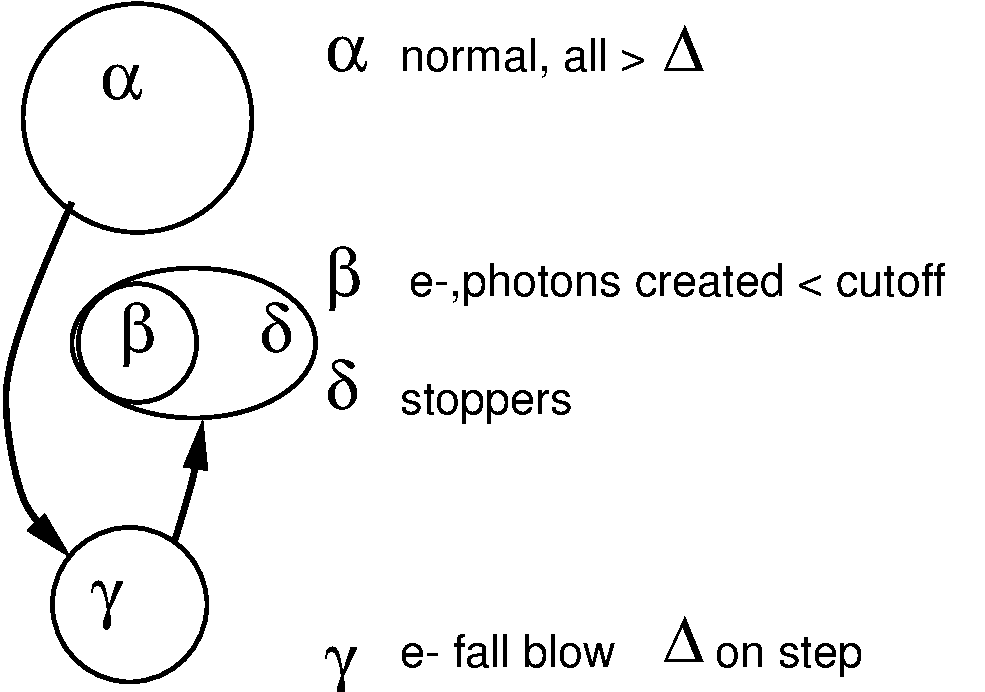
\includegraphics[height=5cm]{figures/sprrz_logic}
\end{center}
\caption[Energy deposition classes in SPRRZnrc]{Modes of energy deposition considered in SPRRZnrc. $\alpha$ events
are those in which energy is deposited by electrons in a step with the
energy entirely above $\Delta$. $\gamma$ events are those in which the
electron starts a step with its energy greater than $\Delta$ and ends with
an energy below $\Delta$. The $\delta$ events are all those events in which
an electron or photon are being terminated because they are below the
cutoffs AE or AP.  This includes a subset of $\beta$ events formed by
electrons and photons which are created with their energy initially below
AE or AP.}
\label{fig_spr_logic}
\end{figure}

The dose delivered by the $\alpha$ events in figure~\ref{fig_spr_logic}
is simple to analyze. In the numerator we just sum the actual energy
deposition. In the denominator we sum the energy deposition times
the ratio of restricted stopping powers at the mid-point energy of the
step, i.e.
\eqn{EDEP \frac{\rspE{Emid}{g}}{\rspE{Emid}{m}}}
This gives how much energy would be deposited in medium $g$ instead of
medium $m$.

The $\beta$ events are not scored at all, except in an evaluation of the
total dose. These events correspond to electrons or photons being created
in the cavity region below the respective transport cut-offs. It is
arguable how to deal with these events, but in traditional calculations
starting from electron spectra they were either ignored or lumped in with
the stoppers.  This issue has been discussed in Borg et al, and there is no
clear solution at this time\cite{Bo99a}.  However, the fraction of the dose contributed
in the cavity region from these events is output by SPRRZnrc and found to
be very small for electron beams or for photon beams at \Co~ energies and
higher. This fact makes the problem academic in most situations.  The
problem becomes serious for low-energy photon beams, but here the
application of Spencer-Attix cavity theory is also suspect\cite{Bo99a}.

The $\delta$ or stopper events which are not $\beta$ events,
are scored as part of the track-end term in
eqn(\ref{eq_sa_spr}).  This is done by scoring the natural energy deposition
in the numerator and the same energy deposition multiplied by the ratio of
the unrestricted stopping powers at $\Delta$ (which are equal to the
restricted stopping powers), i.e.:
\eqn{EDEP \frac{\rspt{g}}{\rspt{m}}.}
Note that this does not merely correspond to the energy deposition in the
second medium, because for a stopper, the energy deposition would be the
same in both media (it just deposits all of its energy which is the same in
both cases). The track-end term in eqn(\ref{eq_sa_spr}) is derived to take
into account that the number of stoppers in each medium will differ because
the fluence of particles stopping in each medium will differ and this
number of stoppers is proportional to the stopping power.

The $\gamma$ events, those particles which cross $\Delta$ during their step
are scored by treating the step as having two components.  The component
with energy above $\Delta$ is treated as if it were an $\alpha$ event and
the component of the energy deposited below $\Delta$ is treated as a
$\delta$ event.

\begin{table}[htb]
\begin{center}
\caption{Energy deposition classes and their components}
\begin{tabular}{|cc|}
\hline
IT value & included events \\
\hline
1  & $\alpha + \gamma + (\delta -\beta)$ \\
3  & $\alpha + \gamma$\\
total & $\alpha + \gamma + \delta$ \\
\hline
\end{tabular}
\end{center}
\end{table}
The SPRRZnrc program scores 3 different doses: the total dose;
dose including everything except the
$\beta$ component (stoppers created below $\Delta$)[IT=1]; dose from
$\alpha$ plus $\gamma$ only [IT=3].
The IT=2 and IT=4 components
correspond to the IT=1 and IT=3 components but scored in the $g$ material
as outlined above. The code then outputs: the total dose; the
fraction of the total dose due to included stoppers (IT=1~$-$~IT=3)/total;
and the fraction of the total dose due to excluded stoppers
(total$-$~IT=1)/total.

The IT=2 dose component is the same as the IT=1 dose component except as
modified to represent the dose in the detector medium as described above.
The IT=4 component similarly corresponds to the IT=3 component, i.e. the
dose less the actual stoppers but including the crossers.

The stopping-power ratios are calculated as the IT=1 dose component divided
by the IT=2 dose component (strictly the scored energy depositions divided
by the respective densities are used).  The stopping-power ratio less the
stoppers is calculated by taking IT=3 divided by IT=4.

The code outputs he two different stopping-power ratios to demonstrate that
the inclusion of the stoppers has only a small effect on the overall
stopping-power ratio, which is a good thing since the treatment of the
stoppers is somewhat arbitrary.  However, it should be pointed out that the
$\gamma$ events are not classified as stoppers but in fact they do contain
some element of the stoppers dose since steps are not stopped at $\Delta$,
but rather at some energy slightly less than $\Delta$.



%\clearpage











\subsection{Input/output control}
\index{SPRRZnrc!I/O control}

I/O control input is delimited between \verb+:start I/O control:+\\
and \verb+:stop I/O control:+.  Most I/O control input
for SPRRZnrc is common to all user codes and is described in
section~\ref{common_I_O_control}\lpage{common_I_O_control}.  However,
the {\tt SPR OUTPUT} control is unique to SPRRZnrc and you input it
as follows:
\begin{verbatim}
  SPR OUTPUT
        = regions         (0)  Specify stopping power ratio output by
                               regions (no .plotdat file will be generated)
        = slabs/cylinders (1)  Specify stopping power ratio output by slabs
                               & cylinders (.plotdat file is generated)
***************************************************************************

  IF SPR OUTPUT= regions

  SPR START REGION   (M)  region numbers in which to start scoring stopping
                           power ratios

  SPR STOP REGION    (M)  region numbers in which to stop scoring stopping
                           power ratios

***************************************************************************

  IF SPR OUTPUT= slabs/cylinders

  SPR IN CYLINDER IX  (M)  Cylinder numbers for which to output
                           stopping power ratios (= 0 for no output)

  SPR IN SLAB IZ      (M)  planar slab numbers for which to output
                           stopping power ratios (= 0 for no output)

**************************************************************************
\end{verbatim}
\index{.plotdat!SPRRZnrc}

\subsubsection{{\tt SPR OUTPUT} options}
\index{SPRRZnrc!SPR OUTPUT}

\index{range rejection!SPRRZnrc}
{\tt SPR OUTPUT} is used to determine how stopping power ratios are
output.  If electron range rejection is off, then stopping power ratios
in all regions are output to the {\tt .egslst} file.  If electron
range rejection is on, then stopping power ratios are zeroed in the
{\tt .egslst} file except in regions specified using
{\tt SPR START REGION} and {\tt SPR STOP REGION} (if
{\tt SPR OUTPUT= regions}) or in slabs/cylinders specified using
{\tt SPR IN CYLINDER IX} and {\tt SPR IN SLAB IZ} (if
{\tt SPR OUTPUT= slabs/cylinders}).  In addition, electron range rejection
is automatically turned off in the regions/slabs/cylinders you have selected
for output so that the stopping power ratios will be meaningful.  If you
are using the {\tt SPR OUTPUT= slabs/cylinders} option, then you will also
get a {\tt inputfile\_dd.plotdat} file which contains the stopping power ratios (and
doses) in the selected slabs and a {\tt inputfile\_rad.plotdat} file
containing stopping power ratios (and doses) in the selected cylinders.
This files are in a format that can be plotted
with {\tt xmgrace} or other plotting program.
\index{.plotdat!SPRRZnrc}

\subsection{Monte Carlo control}
\index{SPRRZnrc!Monte Carlo control}

Monte Carlo control input is delimited between
\verb+:start Monte Carlo inputs:+\\
and \verb+:stop Monte Carlo inputs:+. In addition to the Monte Carlo inputs
common to all user codes (see section~\ref{MC_inputs}\lpage{MC_inputs}),
SPRRZnrc has the following Monte Carlo input:
\begin{verbatim}
  PHOTON REGENERATION         (C)  yes => primary photons are regenerated
                                          after they interact and scattered
                                          photons are thrown away.
                                   no (default) => full calculation

\end{verbatim}
\index{photon regeneration!SPRRZnrc}

\subsubsection{{\tt PHOTON REGENERATION} option}
\index{SPRRZnrc!photon regeneration}
\label{photregsect}

The photon regeneration option is used to calculate the stopping power ratios
for electrons resulting from an unattenuated and unscattered photon beam.
If {\tt PHOTON REGENERATION= yes}, then, prior to a pair production,
compton, photoelectric or Rayleigh event, the properties of the photon about
to interact are saved.  After the interaction, any scattered photons or
photons resulting from relaxation process are discarded and (once all
secondary electrons have been transported) transport reverts to the duplicate
photon that was saved just before the interaction.  In addition, photons
resulting from bremsstrahlung events and positron annihilation events are
eliminated on the spot.
%, and positrons resulting from pair events are
%converted to electrons.
%\note{Why are positrons made into electrons in photon regeneration?}
%\note{Same occurs in general? WHY?????}

This option is to be used when calculating stopping-power ratios for use
in air kerma cavity ion chamber standards since the basic theory makes this
assumption. This makes the calculated stopping-power ratio independent of
the details of the geometry as long as there is full buildup.  This is
discussed in detail by Borg et al\cite{Bo99a}.  This option should not be
used when calculating stopping-power ratios in a phantom since in that case
you want the effects of scatter and attenuation to be taken into effect.


%\renewcommand{\rightmark}{{CAVRZnrc}}
%%%%%%%%%%%%%%%%%%%%%%%%%%%%%%%%%%%%%%%%%%%%%%%%%%%%%%%%%%%%%%%%%%%%%%%%%%%
\section{CAVRZnrc}
%%%%%%%%%%%%%%%%%%%%%%%%%%%%%%%%%%%%%%%%%%%%%%%%%%%%%%%%%%%%%%%%%%%%%%%%%%%
\renewcommand{\leftmark}{{CAVRZnrc}}
\index{CAVRZnrc}

\subsection{Introduction}

CAVRZnrc calculates various factors of interest when using cavity ion
chambers such as $A_{att}$ and $A_{scat}$ and $A_{wall}$.
It has been described in detail in various
publications\cite{Bi85,Ro85a,RB90a,Bi90a} and shown to produce results in
good agreement with standard theory\cite{Bo99a}.

\subsection{Cavity inputs}
\index{CAVRZnrc!cavity inputs}

CAVRZnrc requires an extra set of
inputs defining the cavity region.  These inputs must appear between the
delimiters {\tt :start cavity inputs:} and {\tt :stop cavity inputs:}.

If the user has input the radial geometry using
{\tt METHOD OF INPUT= individual} or {\tt METHOD OF INPUT= groups}
(see section~\ref{geomsect}\lpage{geomsect}), then the following inputs must
appear between the cavity input delimiters:
\begin{verbatim}
   NUMBER OF CAVITY REGIONS (I)   number of geometrical zoneS
                                  comprising the cavity.

   REGION NUMBERS OF THE CAVITY  (M)
                                  the array of these zones
                                  (the cavity region numbers)
\end{verbatim}
Thus, the user defines the cavity in terms of region numbers within the
geometry.

Alternatively, CAVRZnrc offers another method for entering the geometry
in which the geometry is
automatically defined based on cavity information specified by the user.
In this case, only {\tt METHOD OF INPUT= cavity information} needs to be
entered between the {\tt :start geometrical inputs:} and
{\tt :stop geometrical inputs:} delimiters.  Then, between the
cavity input delimiters, the following inputs must be supplied:

\begin{verbatim}

   WALL THICKNESS      (R)   thickness of the chamber walls (cms)
                             (defaults to 0.273)

   CAVITY RADIUS       (R)   outer radius of the cavity (cms)

   CAVITY LENGTH       (R)   length of the cavity (cms) (defaults to 0.2)

   ELECTRODE RADIUS    (R)   radius of the electrode (defaults to 0.)

   WALL MATERIAL       (C)   wall material

   only if   ELECTRODE RADIUS > 0.0
   ELECTRODE MATERIAL  (C)   electrode material
\end{verbatim}
CAVRZnrc creates a simple 3-cylinder
({\tt RCYL(1)=ELECTRODE RADIUS, RCYL(2)=\\CAVITY RADIUS, RCYL(3)=
CAVITY RADIUS + WALL THICKNESS}), 3-slab ({\tt ZPLANE(1)=0,\\
ZPLANE(2)=WALL THICKNESS, ZPLANE(3)=WALL THICKNESS + CAVITY LENGTH,\\
ZPLANE(4)=2*WALL THICKNESS + CAVITY LENGTH}) geometry based on these
inputs.  The material in the cavity is assumed to be AIR.  This option was
useful for early calculations but is not adequate for chambers in which we
want to include much detail.

\subsection{Input/output control}
\index{CAVRZnrc!I/O control}
\label{cavrziosect}

As with the other user codes, I/O control inputs must appear within
the delimiters {\tt :start I/O control:} and {\tt :stop I/O control:}.
In addition to I/O controls that are common to all user codes (see
section~\ref{common_I_O_control}\lpage{common_I_O_control}), CAVRZnrc
has the following inputs:
\begin{verbatim}
  STORE INITIAL RANDOM NUMBERS
        = no          (0)  do not store initial random numbers
        = last        (1)  store initial random number for last history
        = all deposited (2)store the initial random number for all
                           that deposit energy in the cavity
        = all         (3)  store all the initial random numbers

  OUTPUT OPTIONS
        = short              (0)  short output -just the cavity summary
                                  and the dose grid.
        = cavity details     (1)  above plus details for each cavity zone
\end{verbatim}
\index{CAVRZnrc!store initial random numbers}
The {\tt STORE INITIAL RANDOM NUMBERS} input has been included here because
CAVRZnrc has one option, {\tt STORE INITIAL RANDOM NUMBERS= all deposited},
that is not included in the other user codes (see
section~\ref{rnssect}\lpage{rnssect}).
With this option, the initial random numbers from only those histories that
end up depositing energy in the cavity region are stored in the
{\tt .egsrns} file.  Then, if the run is restarted with
{\tt IRESTART= start-RNS} (see section~\ref{restartsect}\lpage{restartsect}),
all histories will end up depositing energy in the cavity region.

\index{CAVRZnrc!output options}
If the user chooses {\tt OUTPUT OPTIONS= short}, then dose and correction
factors will only be output for the cavity as a whole.  If
{\tt OUTPUT OPTIONS= cavity details}, then dose and correction factors
will be output for the cavity as a whole and for each region that makes up
the cavity.

\subsection{Monte Carlo control}
\index{CAVRZnrc!Monte Carlo control}

Monte Carlo control input is delimited between
\verb+:start Monte Carlo inputs:+\\
and \verb+:stop Monte Carlo inputs:+.  In addition to Monte Carlo inputs that
are common to all user codes (see
section~\ref{MC_inputs}\lpage{MC_inputs}), CAVRZnrc had the following
Monte Carlo inputs:
\begin{verbatim}
  IFULL
         = dose and stoppers     (0) just calculate total dose
         = Aatt and Ascat        (1) Above plus Aatt, Ascat
         = Ap                    (2) Above plus Ap as well (option
                                     currently disabled)
         = Afl and <s>g/w        (3) Above plus Afl and <s>g,w as well
                                     (option currently disabled)

  STATISTICAL ACCURACY SOUGHT    (R) % statistical accuracy of the total
                                     dose in the peak region that is
                                     sought The program executes until this
                                     accuracy is obtained or the CPU time
                                     runs out.
  PHOTON REGENERATION
         = yes (1) the calculation is performed with regeneration
                           of the parent photon after they have
                           interacted. A typical setting when FANO
                           conditions are examined.
         = no (0)  a normal calculation.
         = no electrons from wall (ifano = 2) secondary electrons from
                           interactions in the cavity wall are immediately
                           eliminated.  Photons are not regenerated.
                           [IFANO]
\end{verbatim}
\index{photon regeneration!CAVRZnrc}

\subsubsection{{\tt IFULL= dose and stoppers} option}
\index{CAVRZnrc!IFULL}
\index{CAVRZnrc!output of dose}
\label{cavrzifullsect1}

If {\tt IFULL= dose and stoppers}, then CAVRZnrc will output the total
dose in the cavity and, if {\tt OUTPUT OPTIONS= cavity details},
in each region making up the cavity to the {\tt .egslst} file.

\subsubsection{{\tt IFULL= Aatt and Ascat} option}
\index{CAVRZnrc!output of $A_{att}$ and $A_{scat}$}
\label{cavrzifullsect2}

The methods used to calculate the various correction factors have been
described in the literature\cite{Bi85,Ro85a,Bi86,RB90a}.
%\note{This section on Awall needs to be completed .}

If {\tt IFULL= Aatt and Ascat}, then CAVRZnrc will output the total dose,
$A_{att}$, $A_{scat}$ and $A_{wall}$ in the cavity and, if {\tt OUTPUT
OPTIONS= cavity details}, in each region of the cavity to the {\tt
.egslst} file. The listing files also include $K_{wall} = 1./A_{wall}$
(etc).

The scatter correction factor, A$_{scat}$, is defined as the ratio of the
total energy deposited in the cavity to the energy deposited by electrons
generated by primary photon interactions~\cite{Bi86}.  In CAVRZnrc,
photons are flagged as secondary if they have been scattered in compton,
or Rayleigh events, generated by bremsstrahlung or positron annihilation
events, generated by atomic relaxations after compton or photoelectric
events, or if their energy is deposited locally because they have
energy $<$ N-shell energy in a photoelectric event.  Once CAVRZnrc has
totalled the energy deposited in the cavity by electrons generated by
primary photons (ECAV$_{prim}$), and the energy deposited in the cavity
by electrons generated by photons flagged as secondary (ECAV$_{sec}$),
A$_{scat}$ is calculated using the equation:

\begin{equation}
A_{scat}=1+\frac{ECAV_{sec}}{ECAV_{prim}}
\end{equation}

\subsubsection{{\tt STATISTICAL ACCURACY SOUGHT}}
\index{CAVRZnrc!statistical accuracy sought}

If you input a value for {\tt STATISTICAL ACCURACY SOUGHT}
other than zero, then CAVRZnrc will stop when the percent uncertainty on the
total dose in the cavity volume (all cavity regions combined) is equal
to {\tt STATISTICAL ACCURACY SOUGHT} provided that
{\tt NUMBER OF HISTORIES} (see section~\ref{histsect}\lpage{histsect})
or {\tt MAX CPU HOURS ALLOWED} (see section~\ref{cpusect} \lpage{cpusect}) have
not been reached first.

\subsubsection{{\tt PHOTON REGENERATION} options}
\index{photon regeneration!CAVRZnrc}

CAVRZnrc offers two photon regeneration options.  If the user selects
{\tt PHOTON REGENERATION= yes}, then photon regeneration is similar to
that in SPRRZnrc (see section~\ref{photregsect}\lpage{photregsect}).
Unlike SPRRZnrc, where it is required for proper
stopping power ratio calculations as used in primary
air-kerma standards, the purpose of this option in CAVRZnrc is
mainly for theoretical benchmark calculations ({\em e.g} testing
for artefacts under Fano conditions). An additional use
could be for an independent verification of $A_{wall}$: one
runs simulations with {\tt PHOTON REGENERATION= ON} and {\tt PHOTON
REGENERATION= OFF}, the
ratio of the two doses is per definition $A_{wall}$. This is
however not very efficient and a better way to accomplish
this task is to use the cross section enhancement or
photon splitting options described below.

The second regeneration option in CAVRZnrc is {\tt PHOTON REGENERATION= no
electrons from wall}.  With this option, charged particles resulting from
pair production, compton and photoelectric events are eliminated provided
that the interaction did not take place inside the cavity.
This is a hack that has been used to study
the dose fraction from photon interactions in the cavity.

\subsection{CAVRZnrc variance reduction techniques}

\subsubsection{Photon cross section enhancement}
\label{cavrz_cse}
\index{cross section enhancement!CAVRZnrc}
\index{CAVRZnrc!cross section enhancement}

The cross section enhancement technique in CAVRZnrc is
similar to the one implemented in DOSRZnrc
(see section \ref{dosrz_cse} page~\pageref{dosrz_cse}) but
in CAVRZnrc it is applied globally in the entire geometry and the value of
$C_e$ is input directly (as opposed to C as input in the DOSRZnrc case).
Cross section enhancement in CAVRZnrc can be turned on by
including the following line in the input file:
\begin{verbatim}

  CS ENHANCEMENT FACTOR=  some real number [cs_enhance]

\end{verbatim}
If the input is missing or less than unity, there will be
no effect.  But if the enhancement factor is set to greater than unity, the
effect is dramatic: all other user input concerning photon forcing,
splitting, exponential transform, etc., is ignored. In addition,
the calculation result \underline{always} corresponds
to the {\tt IFULL= Aatt and Ascat} option, no matter what the
user requested (but only $A_{wall}$ is calculated,
not the individual $A_{scat}$ and $A_{att}$, see
section \ref{cavrzifullsect2}). In addition, all scoring
is done using proper history-by-history statistics using
the common block {\tt score1}.  The drawback is that dose
and $A_{wall}$ are calculated for the whole cavity and
not on a region-by-region basis as under normal
CAVRZnrc operation.

The following text gives a brief description of the differences
to the DOSRZnrc implementation: The motivation behind the
implementation of cross section enhancement in CAVRZnrc was the desire to
have an independent calculation technique for $A_{wall}$ that is
not too inefficient compared to the unweighting technique. Indeed,
$A_{wall}$ can be calculated by running two separate CAVRZnrc
simulations, one with normal transport  and one with attenuation
and scatter removed via the {\tt photon regeneration= on} option. The ratio of the
cavity dose from the former to the dose from the latter calculation is by
definition $A_{wall}$. Because both calculations
are uncorrelated, their uncertainties add in quadrature and so, the uncertainty
on $A_{wall}$ is larger than the individual dose uncertainties.
The purpose of the cross section enhancement implementation in
CAVRZnrc is to make the two necessary dose calculations at once
and thus reduce the uncertainty of $A_{wall}$ because of the strong
correlation between the ``normal'' dose and the dose with
attenuation and scatter removed. To accomplish this task,
scattered photons are killed as in DOSRZnrc with probability
$1/C_e$. If they survive, they are marked as scattered by setting
their {\tt latch} variable to 3. Unlike in DOSRZnrc, the unscattered
portion of primary photons is always kept on the stack and transported.
However, these non-scattered fractions of primary photons are marked
as attenuated primary photons ({\tt latch=2}) with probability
$1-1/C_e$ and therefore their descendents only contribute to the
dose with attenuation and scatter removed. In addition, scatter,
bremsstrahlung and annihilation from {\tt latch=2} particles are
immediately removed from the stack. It is then clear that
{\tt latch=0,2} electrons contribute to the dose with
attenuation and scatter removed, {\tt latch=0,3} electrons to
the normal dose.

\subsubsection{Photon splitting}
\index{photon splitting!CAVRZnrc}
\index{CAVRZnrc!photon splitting}
\label{cavrzsplitsect}

An additional variance reduction scheme offered in CAVRZnrc
is the photon splitting technique.
Input that turns on photon splitting must appear
between the {\tt :start variance reduction:}
and {\tt :stop variance reduction:} delimiters and is:

\begin{verbatim}

 PHOTON SPLITTING=    (I)    Number of times to split a photon
                             If missing or < 2  => normal transport
                             If >= 2 (allowed only for ifull= dose and
                             stoppers or = Aatt and Ascat), the macro
                             $SELECT-PHOTON-MFP essentially replaces the
                             entire PHOTON routine.
                             [n_split]

\end{verbatim}

This technique is borrowed from Ref. \cite{KF99} where it was shown
to increase the efficiency of external photon beam calculations for
radiotherapy by up to a factor of 5. The increase in CAVRZnrc is
not so dramatic, nevertheless an increase in the efficiency
of cavity dose calculations of up to a factor of 3 compared to using photon
forcing has been observed.

This option is only available with {\tt IFULL= dose and stoppers or =Aatt and Ascat}.
It is also possible to use the {\tt ifano} option (only
if {\tt IFULL=0}). Note that with photon splitting
on, all scoring
is done using proper history-by-history statistics using
the common block {\tt score1}.  The drawback is that dose
(and $A_{wall}$ if requested) are calculated for the whole scoring cavity and
not on a region-by-region basis as under normal CAVRZnrc operation.

The algorithm works as follows:
each photon that is to be transported is split into
{\tt n\_split} photons with weights $w_0/${\tt n\_split}
($w_0$ is the original photon weight). The number of
mean-free-paths $\lambda_i$ to the next interaction of the $i$'th
such photon is sampled from
\begin{equation}
\lambda_i = -\ln \left[1 - {\xi + i - 1 \over {\tt n\_split} } \right]
\end{equation}
where $i$ runs from 1 to {\tt n\_split} and where $\xi$ is a random
number. This forces a uniform distribution of interaction sites.
In addition we have $\lambda_{i+1} > \lambda_i$ and therefore
only transport from $\lambda_i$ to $\lambda_{i+1}$ is needed to
get to the interaction site of the $i+1$'st photon from the
interaction site of the $i$'th photon. When one of the split-photons
interacts, all resulting scattered photons are killed with probability
1/{\tt n\_split} and marked as scattered if they survive
({\tt latch=3}). If {\tt IFULL= Aatt and Ascat} or {\tt photon
regeneration= on}, the original photon is
re-created at each interaction site with probability
1/{\tt n\_split} and marked as a regenerated photon ({\tt latch=2}).
As for the cross section enhancement technique, {\tt latch=0,3} particles
contribute to the normal dose, {\tt latch=0,2} particles to the dose
with attenuation and scatter removed. The ratio of the two is
$A_{wall}$ and so, photon splitting is a third independent
technique for calculating this quantity.

A rule of thumb for good efficiency is to use
\eqn{n\_split \ge \frac{N_o}{1. - e^{-\lambda}} }
where $\lambda$ is approximately the number of photon mean free paths in the
geometry of interest and $N_o \ge 5$. For $^{60}$Co, $\lambda$ is about
0.06 for 1 g/cm$^2$ of graphite and so $n\_split$ should be $\ge 80$.

%%%%%%%%%%%%%%%%%%%%%%%%%%%%%%%%%%%%%%%%%%%%%%%%%%%%%%%%%%%%%%%%%%%%%%%%%%%%%
\section{Spherical user codes}
%%%%%%%%%%%%%%%%%%%%%%%%%%%%%%%%%%%%%%%%%%%%%%%%%%%%%%%%%%%%%%%%%%%%%%%%%%%%%

\subsection{Introduction}

Since 2003, the EGSnrc distribution includes a pair of spherical
geometry user codes.
CAVSPHnrc is the spherical analogue of CAVRZnrc, designed for ion chamber
calculations, and has been used extensively for this purpose (see, \eg,
references\cite{Bi90b,RT99}). The other code, EDKnrc, was derived from
SCASPH, an EGS4 user code for the calculation of mono-energetic energy
deposition kernels\cite{Ma88}. EDKnrc has been extended to allow the use
of both monoenergetic and polyenergetic sources.

Both user codes share most of the common features of the RZ user codes
excluding geometry and source types. We will describe these two in the
following subsections and the user is refered to section \ref{Common}
for information on the common input blocks of these codes.

\subsection{Geometry and Material Inputs}

\subsubsection{Geometrical input: spheres and cones}

The geometrical regions subtended by concentric spheres and cones
originating at the common center of the spheres are shown in figure
\ref{fig_spherical}. NR represents the number of spheres and NC the
number of cones. In what follows we explain the input specification of
the geometry.


\begin{figure}[hbt]
\htmlimage{scale=1.2}{}
\begin{center}
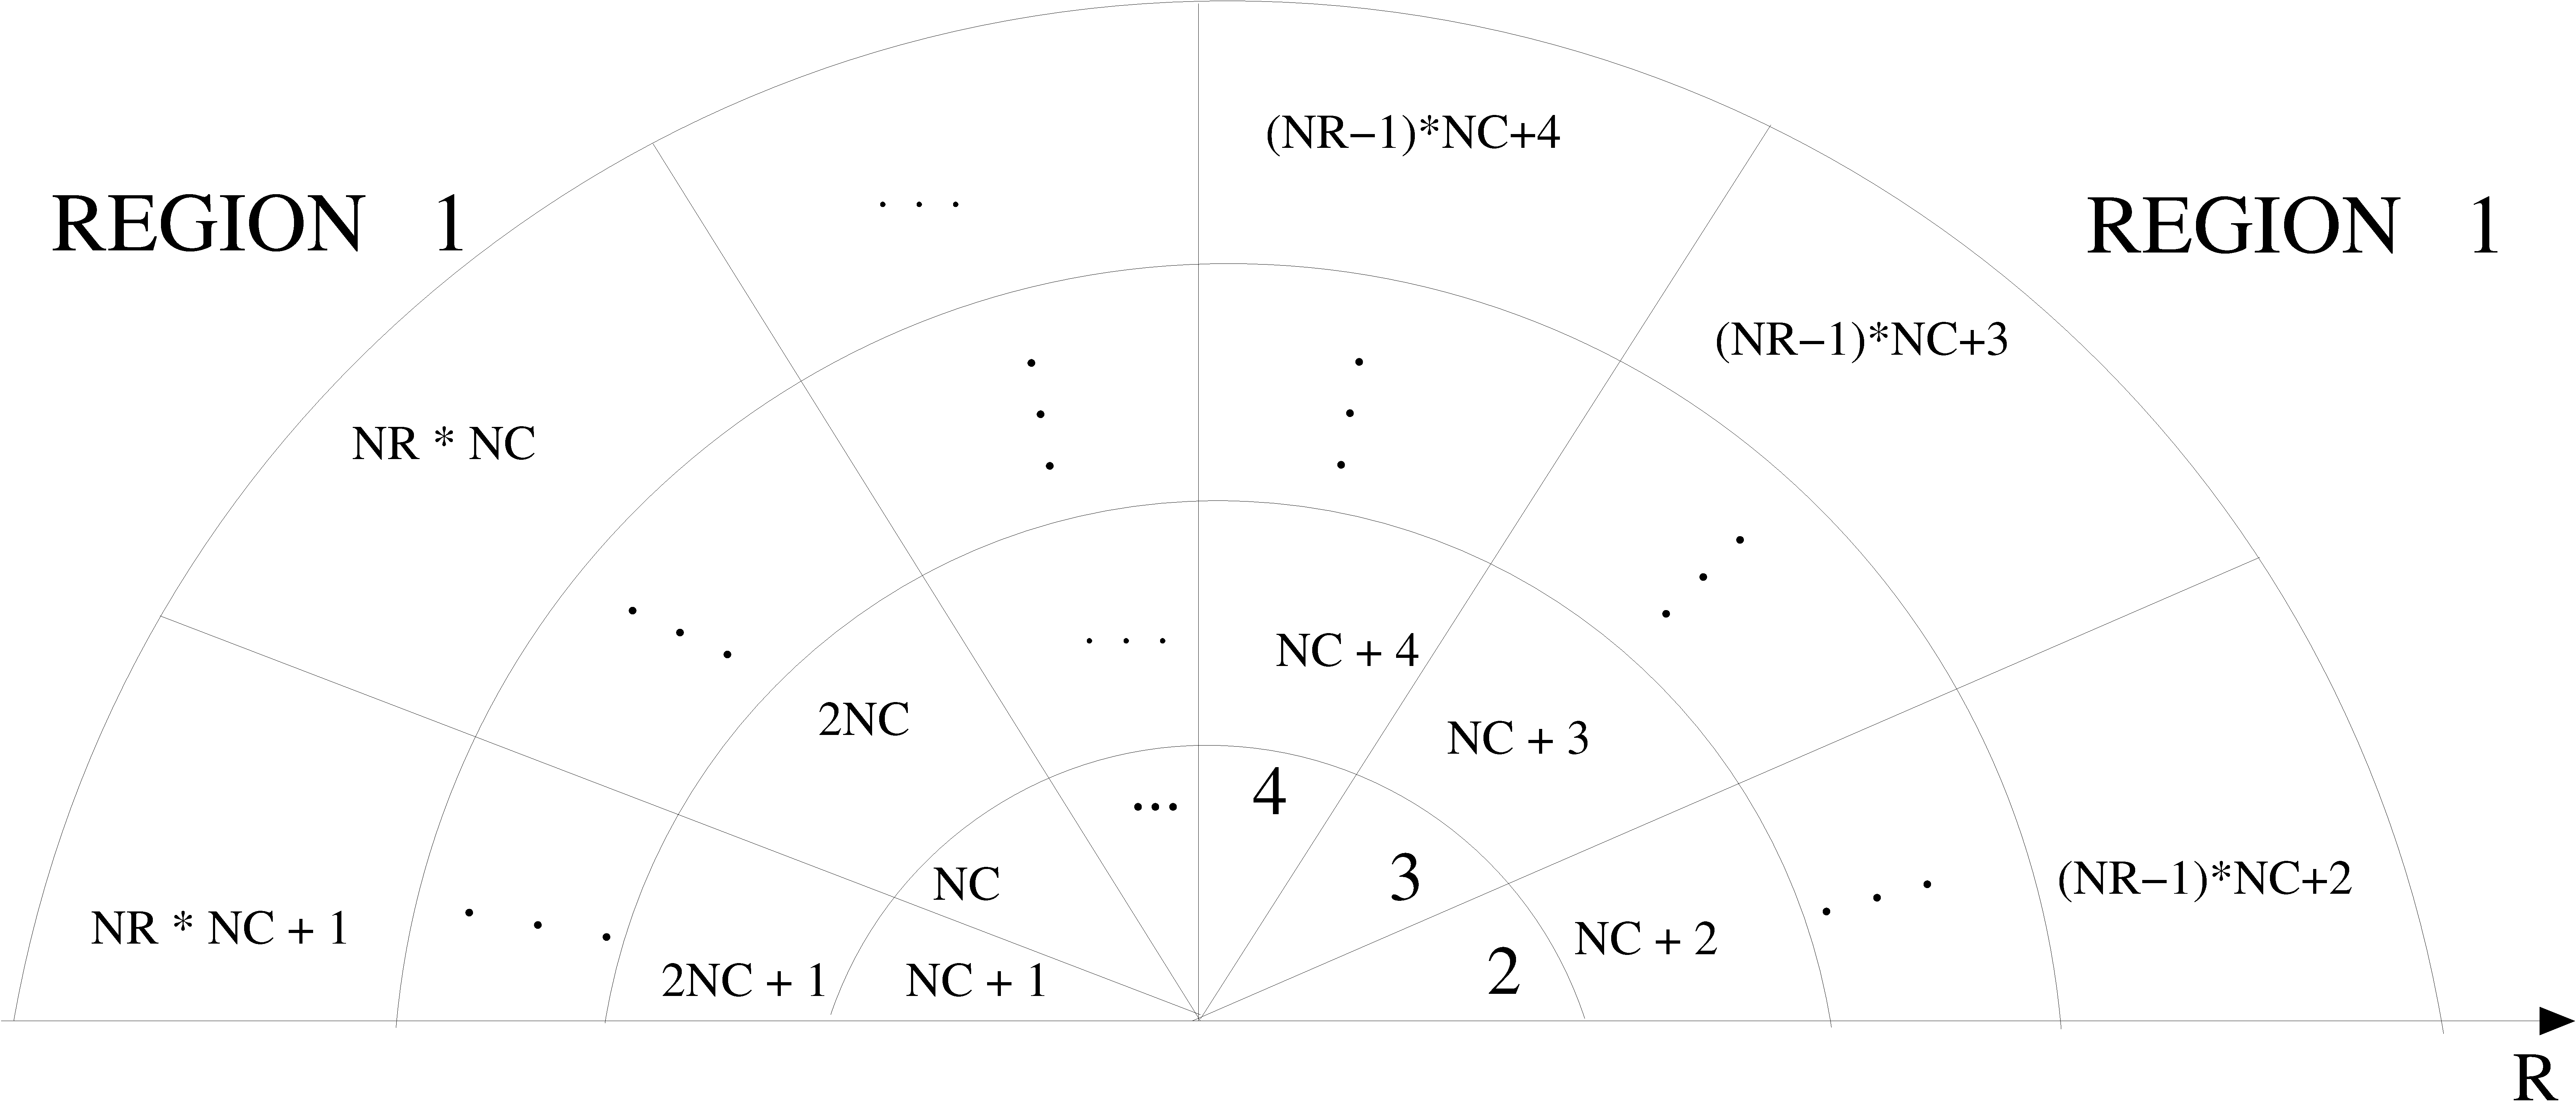
\includegraphics[height=5cm]{figures/spherical}
\end{center}
\caption[Spherical geometry]{Region numbering scheme for the spherical
user codes.  Region number 1 is always outside the geometry. The first
region (2) is defined by the innermost sphere and the cone with the
smallest opening angle. {\tt NR} is the number of radial zones = \# radii
and {\tt NC} = number of cones (0 for purely spherical geometry). }
\label{fig_spherical}
\end{figure}

As in the RZ codes, the geometry inputs are delimited by the strings
{\tt :start geometrical inputs:} and {\tt:stop geometrical inputs:}. The
meaning of the inputs depends on the entries for {\tt NUMBER OF CONES}  and
{\tt NUMBER OF SPHERES}. If a single value is input, then the user is
expected to input the individual corresponding radii or angles. If multiple
values are given for {\tt NUMBER OF CONES}  and/or {\tt NUMBER OF SPHERES},
the user is expected to put in groups of equal angles and/or radii.
If, for instance, several
entries are made for the number of angles, \ie, {\tt NANG1, NANG2, ...}, it
is assumed that the first {\tt NANG1} cones will have the same opening angle
and so on. For spheres, if the user omits the number of radii, it is
assumed that individual entries will be made (after all,
these are user-codes for spherical problems).

\begin{verbatim}
 NUMBER OF CONES= [NANG(1)[,NANG(2),...,NANG(K)]]
                  # If omitted or ZERO, pure spherical geometry assumed
 NUMBER OF SPHERES= [NRAD(1)[,NRAD(2),...NRAD(J)]]
                  # no needed for individual input
\end{verbatim}

Once the user has defined the number of spheres and cones in the problem, the
actual values for the radii and angles must be entered, using the keywords
outlined below:

\begin{verbatim}
RADII= RAD(1), RAD(2), ...RAD(j)
                  #radii of spheres defining the geometry
                  #For group input there must be as many entries
                  #as for the NUMBER OF SPHERES, i.e. :
                  #         J = j
                  #For individual input, NRAD(1) must be equal
                  #to the number of entries, i.e.:
                  #        NRAD(1) = j
                  #unless NUMBER OF SPHERES is omitted, in which case
                  #indiviual input is automatically assumed.
ANGLES= ANG(1), ANG(2),...,ANG(3)
                  #The same rules apply for angles as for radii apply.
\end{verbatim}

One can also enter a group of regions to be considered as the cavity
of a spherical ion chamber and the total dose in these regions will
be computed. For CAVSPHnrc, quantities such as
$K_{att}$ and $K_{scat}$ and $K_{wall}$ are also calculated for the
whole cavity. The specification for the cavity inputs is:
\begin{verbatim}
CAVITY ZONES= [REG1[, REG2...,REGn]] #geometrical zones defined as the
                                     #cavity (real numbers)
\end{verbatim}

\subsubsection{Material input.}

These codes have a simple structure for entering the material input. First
the user must provide a list of media in the problem where the first
medium is taken as default, \ie, every region is considered to have this
medium. Then, medium numbers for all regions where the medium is not
medium 1 must be specified.


\begin{verbatim}
 MEDIA= MEDIUM1, MEDIUM2,..., MEDIUMn

 MEDNUM=        MEDIUM2, MEDIUM2, MEDIUM3,..., MEDIUMn
 START REGION=  START1,  START2,  START3,...,  STARTn
 STOP REGION=   STOP1 ,  STOP2,   STOP3, ...,  STOPn

\end{verbatim}

\subsection{CAVSPHnrc}
The NRC user code CAVSPHnrc (spherical geometry) like CAVRZnrc
(cylindrical geometry) calculates various factors of interest when using
ion chambers such as $K_{att}$, $K_{scat}$, $K_{wall}$ and the dose to the
cavity region per unit incident fluence.

The input file for this user code is very similar to the one for
CAVRZnrc. Only two input blocks are different, the geometry input block
and the input block for the sources. The geometry input was described
previously and the input for the sources differ from CAVRZnrc, in that
only four source types are available: a parallel beam from any angle
(source 0), a point source from any angle (source 1), a parallel beam
from any angle with radial distribution (source 10), a point source from
any angle with radial distribution (source 11).
and a point source from any angle. The source input block is defined by
the delimeters {\tt :start source inputs:} and {\tt :stop source inputs:}
and the same inputs are needed as in CAVRZnrc (see
section~\ref{source_inputs} on page~\pageref{source_inputs}).  In
particular, one must define:

\begin{verbatim}
  INCIDENT PARTICLE= electron   (-1)  electrons
                     photon     (0)   photons
                     positron   (1)   positrons

  SOURCE NUMBER                 (I)   number of the source
                                      [ISOURC]
  SOURCE OPTIONS                (M)   four or five real numbers as specified
                                      below

------------------------------------------------------------------------------

 SOURCE 0/10:  FOR PARALLEL BEAM FROM ANY ANGLE (10-->WITH RAD. DISTN)
              RBEAM,UINC,VINC,WINC
               RBEAM   RADIUS OF THE BEAM AT THE FRONT OF THE TARGET IN CM
                               DEFAULTS TO MAX RADIUS
               UINC    INCIDENT X-AXIS DIRECTION COSINE
               VINC    INCIDENT Y-AXIS DIRECTION COSINE
               WINC    INCIDENT Z-AXIS DIRECTION COSINE
                       NOTE: (UINC,VINC,WINC) GET AUTOMATICALLY NORMALIZED
                             DEFAULTS TO (0.0,0.0,1.0)
------------------------------------------------------------------------------

 SOURCE 1/11:  FOR POINT SOURCE INCIDENT FROM ANY ANGLE (11-->WITH RAD. DISTN)
             DISTR,RBEAM,UINC,VINC,WINC
               DISTR   DISTANCE OF THE SOURCE FROM THE MIDDLE OF THE TARGET
                       IN CM (DEFAULTS TO 100.)
               RBEAM   RADIUS OF THE BEAM AT THE FRONT OF THE TARGET IN CM
                               DEFAULTS TO MAX RADIUS
               UINC    INCIDENT X-AXIS DIRECTION COSINE
               VINC    INCIDENT Y-AXIS DIRECTION COSINE
               WINC    INCIDENT Z-AXIS DIRECTION COSINE
                       NOTE: (UINC,VINC,WINC) GET AUTOMATICALLY NORMALIZED
                             DEFAULTS TO (0.0,0.0,1.0)
------------------------------------------------------------------------------

 SOURCE 10 OR 11:
       SPECIFY MODE:
               MODE = local (0)     IF RADIAL DISTRIBUTION IS TO BE INPUT
                                    LOCALLY WHETHER THROUGH THE KEYBOARD
                                    (INTERACTIVE USE) OR THROUGH THE
                                    .INP FILE (DEFAULT)
                    = external (1)  IF THE DISTRIBUTION IS TO BE INPUT
                                    VIA AN EXTERNAL FILE
       IF MODE=local SPECIFY:

           RDISTF(I)= TOP OF RADIAL BIN I FOR I=1,NBIN
           RPDF(I)= PROBABILITY OF INITIAL PARTICLE BEING IN BIN I FOR
                    I=1,NBIN.

                      PROBABILITIES DO NOT NEED TO BE NORMALIZED
                      BUT SHOULD BE IN UNITS CM**-2

       IF MODE=external SPECIFY:

           RDIST FILNAME = FILENAME(WITH EXT) CONTAINING THE ABOVE INFORMATION


       SPECIFY:
           DISTRIBUTION DATA = NONE => NO DISTRIBUTION DATA IN OUTPUT SUMMARY
                             = OUTPUT SUMMARY => INCLUDE DISTRIBUTION
                               DATA IN OUTPUT SUMMARY
\end{verbatim}

\subsection{EDKnrc}

The NRC user code EDKnrc can be used to calculate Energy Deposition Kernels
for photons or electrons (monoenergetic or polyenergtic) forced to interact
at the centre of a spherical
geometry\cite{Ma05}.  The code can output energy deposition kernels (EDK),
dose distributions in the phantom or the dose to regions defined as the
cavity of a spherical ion chamber.  Voxels are defined by the intersection
of a spherical shell with two cones. See figure \ref{fig_spherical}
for more details.

Although the geometry inputs for this user code are similar to CAVSPHnrc,
there are some major differences in other inputs. The input block for I/O
control, defined by the delimeters {\tt :start I/O control:} and
{\tt:stop I/O control:}, is severely abbreviated.  It includes an entry,
{\tt PRINT OUT EDK FILE} that defines whether energy deposition
kernels will be output in the same format as the ones calculated by
Mackie {\it et al.}\cite{Ma88}. The entire input for this block
is shown below:

\begin{verbatim}

:start I/O control:
  IRESTART
       = first    (0) First run for this data set
       = restart  (1) Restart a previous run
       = analyze  (3) Just read in the raw data and do the statistical analysis
       = parallel (5) Combine results from previous parallel runs
  STORE DATA ARRAYS
       = yes             (0) Store data arrays for re-use
       = no              (1) don't store them
  PRINT OUT EDK FILE
       = yes             (0) EDK stored in old format files
       = no              (1) don't produce EDK files in old format
:stop I/O control:
\end{verbatim}


The input block defining Monte Carlo parameters (delimited by
{\tt start}/{\tt stop Monte Carlo inputs:}) is also abbreviated.  Here
one specifies only the number of histories, the initial random number
seeds, and a variable {\tt IFULL}, which specifies the type of calculation,
and an input specifying whether doppler broadening is to be taken into
account during Compton interactions.

\begin{verbatim}

IFULL= cavity calculation        #(0) calculate dose in cavity regions
     = energy deposition kernels #(1) calculate and output EDK's
     = dose calculation          #(2) calculate and output dose
     = dose and edk              #(3) calculate and output EDK's and dose

DOPPLER BROADENING= On
                  = Off

\end{verbatim}

EDKnrc allows for only three possible sources: 1) a photon source algorithm
that forces photons moving along the Z-axis to interact at the origin
(source 0) 2)
an isotropic point source at the origin for any type of
particle (source 1) 3) same as source 0 but with interaction point shifted
to a user-specified position on the Z-axis (source 2).  Source 2
was left for comparison with older EDK calculations, but the user
is strongly discouraged from using it, since it has been shown to produce
numerical artifacts when computing EDK's. For accurate EDK calculations
source 0 should be used.   The inputs specifying the source type, which is
included within the {\tt start}/{\tt stop Source Inputs:} delimiters,
are shown below:

\begin{verbatim}
SOURCE NUMBER= 0 | 1 | 2
#     0 ==>  Photon moving along Z axis forced to interact at origin
#     1 ==>  Point source at origin, isotropically radiating into 4 Pi
#     2 ==>  Same as 0 but interaction point as in old code

# if SOURCE NUMBER= 2
    ZIN      #-> source offset on Z-axis
             #   Option used to emulate old way of calculating EDK
\end{verbatim}

Note that in the case of source 0 or source 2, the {\tt INCIDENT PARTICLE=}
(standard for all user codes when specifying the source) input must be
set to {\tt PHOTON}.

The energy deposited in the geometry can be separated into different
contributions from each photon scattering order (\eg~ primary,
first scatter, second scatter, multiple scatter and radiative). For
electrons, the deposited energy can be split into primary and radiative
contributions. In the standard output file {\tt *.egslst}, only the total
and primary components are written. ONLY if the user selects the option
for creating old format EDK files, all components are stored to a file
following the convention:
\begin{itemize}
\item {\tt edk[EIN].keV}, for monoenergetic sources,
where EIN is the initial energy in keV.
\item {\tt file\_name.keV}, for polyenergetic sources (spectrum),
where {\tt file\_name} is the standard output file name

\end{itemize}

The user also has the choice to
create xmgrace plot files for the {\bf total dose} by using the input block for plot control delimited by
{\tt :start plot control:} and {\tt:stop plot control:}. A description of this input block is
given below:

\begin{verbatim}
   :start plot control:

   PLOTTING
          = Off         (0)   no plots or plot files to be prepared
          = Histogram   (1)   histogram plotting
          = Point       (2)   xy graph


  ONLY IF not PLOTTING= Off

   PLOT RADIAL REGION IX  (M)  radial regions to plot vs angle
                               (= 0 for no plots)

   PLOT CONICAL REGION IC  (M)  angular intervals to plot vs radius
                               (= 0 for no plots)

   :stop plot control:
\end{verbatim}

Plots in radial regions are written to the file {\tt inputfile.angplot}
({\em i.e.} dose versus angle) and plots in conical regions are written
to the file {\tt inputfile.radplot}.

The output capabilities of this user code are very limited but can be
easily extended to print out all components of the energy deposition
kernels.

\typeout{}
\typeout{***Start of Cited References****}
\typeout{}
\renewcommand{\leftmark}{{REFERENCES}}
\renewcommand{\rightmark}{{REFERENCES}}
\section{References}
\vspace*{-1.7cm}
\bibliography{../irs}
%above points to where we find the master reference list
\typeout{}
\typeout{******REMEMBER to create .bbl  and reset twice**********}
\typeout{}
\bibliographystyle{unsrt}


\newpage
\typeout{**********starting index here******************}
\renewcommand{\leftmark}{{Index}}
\renewcommand{\rightmark}{{Index}}
\addcontentsline{toc}{section}{\numberline{}Index}
\setlength{\baselineskip}{0.5cm}


%%%%%%%%%%%%%%%%%%%%%%%%%%%%%%%%%%%%%%%%%%%%%%%%%%%%%%%%%%%%%%%%%%%%%%%%%%%%%%%
%
%  EGSnrc user codes manual
%  Copyright (C) 2021 National Research Council Canada
%
%  This file is part of EGSnrc.
%
%  EGSnrc is free software: you can redistribute it and/or modify it under
%  the terms of the GNU Affero General Public License as published by the
%  Free Software Foundation, either version 3 of the License, or (at your
%  option) any later version.
%
%  EGSnrc is distributed in the hope that it will be useful, but WITHOUT ANY
%  WARRANTY; without even the implied warranty of MERCHANTABILITY or FITNESS
%  FOR A PARTICULAR PURPOSE.  See the GNU Affero General Public License for
%  more details.
%
%  You should have received a copy of the GNU Affero General Public License
%  along with EGSnrc. If not, see <http://www.gnu.org/licenses/>.
%
%%%%%%%%%%%%%%%%%%%%%%%%%%%%%%%%%%%%%%%%%%%%%%%%%%%%%%%%%%%%%%%%%%%%%%%%%%%%%%%
%
%  Authors:         Dave Rogers
%                   Iwan Kawrakow
%                   Jan Seuntjens
%                   Blake Walters
%                   Ernesto Mainegra-Hing
%
%  Contributors:    Frederic Tessier
%
%%%%%%%%%%%%%%%%%%%%%%%%%%%%%%%%%%%%%%%%%%%%%%%%%%%%%%%%%%%%%%%%%%%%%%%%%%%%%%%


\documentclass[12pt,twoside]{article}  %indexm doesn't work with two
					%sides
%\usepackage{supertab}%this didn't work for some reason?
%\usepackage{overcite}			%comment out for html?

\usepackage{moreverb}	%this is used for the boxedverbatim environment
			%used to box the listing files for tutor programs

\setlength{\textwidth}{16.51cm}
%\setlength{\textheight}{23.2cm}
\setlength{\textheight}{23.5cm}
\setlength{\oddsidemargin}{0.0in}
\setlength{\evensidemargin}{0.0in}
\setlength{\topmargin}{-1.5cm}
\setlength{\parindent}{1.5em}
\setlength{\topsep}{0ex}
\setlength{\itemsep}{0ex}

\newcommand{\lpage}[1]{(page~\pageref{#1})}
\newcommand{\Mol}{Moli\`ere}

\newcommand{\Co}{$^{60}$Co}
\newcommand{\parsp}{~\hspace*{1.5em}}
\setlength{\parskip}{0.1in}
\setlength{\baselineskip}{1.0cm}
\newcommand{\head}[1]{\begin{center}\begin{Large}{\bf #1}
                                              \end{Large}\end{center}}
\newcommand{\cen}[1]{\begin{center} #1 \end{center} }
\newcommand{\etal}{{\em et.al.}}
\newcommand{\ie}{{\em i.e.}}
\newcommand{\etc}{{\em etc.}}
\newcommand{\viz}{{\em viz.}}
\newcommand{\eg}{{\em eg.}}
\newcommand{\sprt}[2]{\left(\frac{\overline{L}}{\rho}\right)^{\rm #1}_{\rm #2}}
\newcommand{\eqn}[1]{\begin{equation} #1 \end{equation} }
\newcommand{\rsp}[1]{\left( \frac{L(\Delta)}{\rho} \right)_{#1}}
\newcommand{\PhiT}{\Phi_{\rm T}}
\newcommand{\rspt}[1]{\left( \frac{S(\Delta)}{\rho} \right)_{#1}}
\newcommand{\rspE}[2]{\left( \frac{L({\rm #1})}{\rho} \right)_{#2}}

\newcommand{\note}[1]{\mbox{}\\ \noindent \rule{16cm}{0.5mm} \\
{\em #1} \\ \noindent \rule{16cm}{0.5mm}\\
\typeout{******note: #1 *****}
}

%\newcommand{\indexm}[1]{\index{#1}}
%\typeout{~~~~~~~~~~~~***margin index feature OFF*****************************}
%\typeout{~~~~~~~~~~~~***margin index feature OFF*****************************}
%\typeout{~~~~~~~~~~~~***margin index feature OFF*****************************}
\newcommand{\indexm}[1]{\marginpar{{\sf {\tiny I:#1} }}\index{#1}}
\makeindex


\renewcommand{\refname}{}

%       some commands to get 4 levels in the table of contents and
%       number down to paragraphs
\setcounter{secnumdepth}{4}
\setcounter{tocdepth}{4}
\renewcommand{\thesubsubsection}{\thesubsection.\arabic{subsubsection}}
\renewcommand{\theparagraph}{\thesubsubsection.\roman{paragraph}}
%\renewcommand{\theequation}{\arabic{subsection}.\arabic{subsubsection}.\arabic{equation}}



%\usepackage{html}
\usepackage{graphicx}
%\usepackage{epsf}
%\input{epsf}
\usepackage{longtable}

\usepackage{fancyhdr}
\renewcommand{\footrulewidth}{0.4pt}
\renewcommand{\headrulewidth}{0.4pt}

\lhead[{\sffamily \thepage}]{{\sffamily NRC User Codes for EGSnrc }}
\rhead[{\sffamily NRCC Report PIRS-702}]{{\sffamily ~\thepage}}
%\rfoot[{\sffamily {\rightmark}}]{{\sffamily {\rightmark}}}
\rfoot[]{{\sffamily {\rightmark}}}
% \lfoot[{\sffamily {\leftmark}}]{{\small Last edited $Date: 2013/09/24 18:04:14 $
\lfoot[{\sffamily {\leftmark}}]{{\small Last edited 2011/05/03 15:50:14
}}
\cfoot{}

\usepackage{hyperref}
\hypersetup{colorlinks=true, citecolor=blue, linkcolor=blue, filecolor=blue, urlcolor=blue}
\urlstyle{same}

\usepackage{html}



\begin{latexonly}
\typeout{***Have turned off overfull and underfull messages****}
\tolerance=10000        %suppress Overfull only
\hbadness=10000         %suppress Overfull and Underfull for text (horizontal)
\vbadness=10000         %suppress Overfull and Underfull for vertical "boxes"
\end{latexonly}


\begin{document}

\begin{htmlonly}
For information about the authors and/or institutions involved with this
work, use the links provided in the author list.\\

\begin{rawhtml}
<br><br>
\end{rawhtml}


Postscript versions of the entire paper are available.  You may have to
download the compressed version to disk, uncompress or gunzip them and
then read or print them.\\
\begin{center}
\htmladdnormallink{(uncompressed version 2.4 Mb)}{pirs702.ps}\\
\htmladdnormallink{(gzip version 230 kb)}{pirs702.ps.gz}\\
\htmladdnormallink{(pdf version 440 kb)}{pirs702.pdf}\\
\end{center}
\begin{rawhtml}
<br><br>
\end{rawhtml}

Use the Up button to get back to this page from within the document.
\begin{rawhtml}
<BR> <HR> <P>
\end{rawhtml}
\copyright
Copyright 2021,  National Research Council of Canada
Ottawa
\begin{rawhtml}
<BR> <HR> <P>
\end{rawhtml}
\end{htmlonly}

\pagestyle{empty}

\title{NRC User Codes for EGSnrc}

\begin{center}
{\sffamily \bfseries {\Huge NRC User Codes for EGSnrc}
\vspace{5mm}\\}
\begin{Large}
D.W.O. Rogers, I. Kawrakow, J.P. Seuntjens,  B.R.B. Walters and E.
Mainegra-Hing \\
\end{Large}
Ionizing Radiation Standards,
National Research Council Canada, Ottawa, Canada\\


\vspace{3mm}
{\bfseries
\today}
%January 2010}
\vspace{3mm}\\
\hfill NRCC Report {\sf PIRS-702(revC)} \vspace*{2mm}\\

\begin{figure}[h]
\htmlimage{scale=1.2}{}
\begin{center}
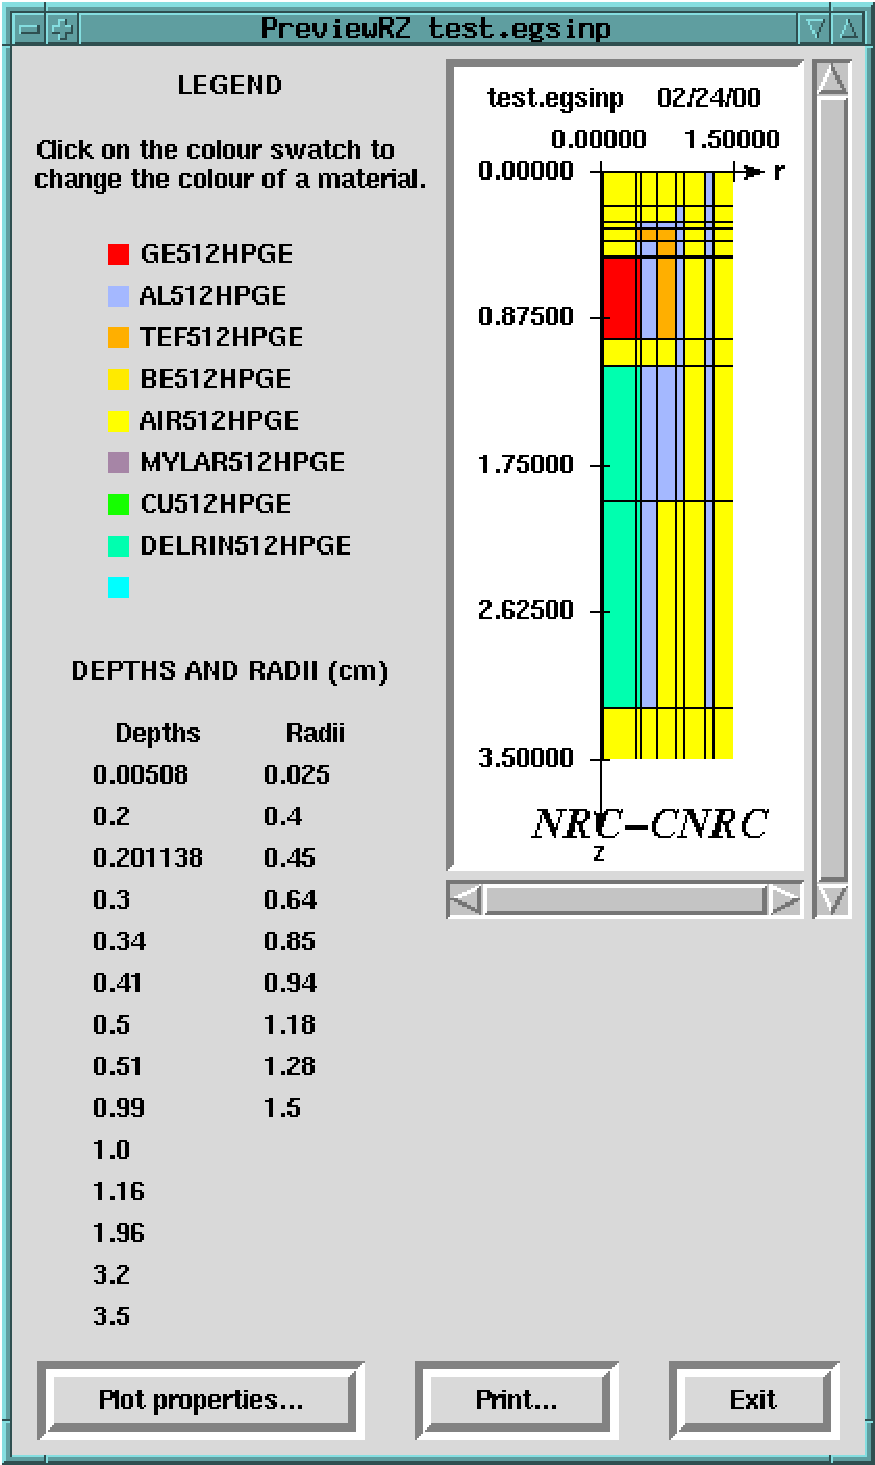
\includegraphics[height=12cm]{figures/PreviewRZ_example}
\\Preview of an RZ geometry in DOSRZnrc.
\end{center}
%\caption{Preview of an RZ geometry in DOSRZnrc.}
%\cen{Get a figure from preview tcl of DOSRZnrc}
\end{figure}

\vfill
\begin{latexonly}
\end{latexonly}

\copyright NRC Canada, 2021
\end{center}
\newpage   %Blank page behind cover
\mbox{}

%\note{This page is intentionally blank to be the back of the front cover.
%Remove this note prior to printing!!!}

\setlength{\baselineskip}{0.5cm}
\newpage

\pagestyle{fancy}
\pagenumbering{arabic}
\setcounter{page}{1}


\begin{abstract}
\label{abstract}
This manual describes the NRC User codes DOSRZnrc, CAVRZnrc, FLURZnrc and
SPRRZnrc which all work with the EGSnrc Code system for Monte Carlo
transport of electrons and photons (see NRC REPORT PIRS--701, ``The EGSnrc
Code System''). There is a graphical user interface available for creating
the inputs to these codes (described separately).

\end{abstract}

%\newpage

\setlength{\baselineskip}{0.1cm}

\tableofcontents

%\newpage
\listoftables
\listoffigures

\setlength{\baselineskip}{0.5cm}

\newpage

\renewcommand{\leftmark}{{INTRODUCTION}}
\section{Introduction}
\subsection{Intent of this report}

Over the years, NRC has developed and distributed a series of user codes
for use with the EGS4 code system for the Monte Carlo simulation of photon
and electron transport.  These have been widely used and their results
compared to experiment in many cases.  However, the codes themselves have
never been properly documented and described. It is the purpose of this
manual to provide a document which describes
both how these codes work and also how a user uses them.  It is not the
purpose of this manual to discuss selection of parameters when using these
codes for a particular application since this is a huge undertaking and is
covered in the already extensive literature on EGS.

Recently, the codes
have been reworked to use the new EGSnrcMP system\cite{Ka03}. This
has increased the flexibility of these codes, including the ability
to run them on both Unix/Linux and Windows systems.

The codes involved in this report are all for
cylindrical RZ and spherical geometries. These are:
\begin{description}

\item[DOSRZnrc] which scores dose in a generalised cylindrical geometry.

\item[FLURZnrc] which scores particle fluence in the same geometry.

\item[CAVRZnrc] which is similar to DOSRZnrc but also scores a variety of
quantities which are of specific interest to dosimetry
calculations for an ion chamber.

\item[SPRRZnrc] which calculates Spencer-Attix spectrum averaged
stopping-power ratios for arbitrary media.

\item[CAVSPHnrc] which is identical to CAVRZnrc but for spherical
geometries.

\item[EDKnrc] which calculates energy deposition kernels for photons
or electrons forced to interact at the centre of a spherical phantom.
It can also calculate dose distributions in the entire phantom or the
dose to specific regions defined as the cavity of a spherical ion chamber.

\end{description}

This manual does not describe the BEAM code for modelling radiotherapy
accelerators, \Co~ units and x-ray systems. BEAM is described
elsewhere\cite{Ro95,Ro98a}. The user codes
described here all have the capability of using either a BEAM generated phase
space file or a full BEAM simulation (compiled as a shared library)
as the source of incident particles.

Also, this manual does not describe the EGS\_Windows system for doing 3D
displays of EGS simulations. EGS\_Windows is described in detail in its own
manual\cite{TR99a}.

\subsection{History}
\index{history}
These codes have a long history at NRC and were first written to work
with EGS3 which was written in Mortran2.  The first germs of these
codes were written by Alex Bielajew who was responsible for coding
CAVRZ as a research tool for work related to ion chamber dosimetry.
This then grew into DOSRZ which strips out some of the special purpose
parts of CAVRZ but adds various more general purpose facilities such as
calculating response functions for detectors. Dave Rogers took these
codes and developed a general purpose fluence scoring code FLURZ and
finally SPRRZ was developed.  Along the way various summer students worked
under Dave Rogers and Alex Bielajew to add features.

One problem was that
all the codes had grown on their own with various bits and pieces being
patched in whenever they were needed for a particular research project.
The system of codes was getting more and more difficult to maintain
and various options failed to work on new systems as they came along
(eg the output listing from FLURZ didn't work on Unix systems
because it was based on a
Digital Vax Fortran extension which was not commonly available on unix
Fortran compilers).  This was overcome in the DOSRZ code by some horrific
coding tricks which made it impossible to change the outputs.  Furthermore the
input files became almost impossible to create since they were just a
large file of numbers where the meaning of each number was dependent on
its position, and often meant different things for the different codes.

To overcome these shortcomings, a major revamping was undertaken in 1998
by Aaron Merovitz, a summer student working for Dave Rogers.  Firstly he
created some general purpose output routines which worked for standard
compilers. Also, as much as possible all graphical output was done through
a single subroutine called {\tt xvgrplot} so that if changes in plotting
output are required. it needs to be changed in only the subroutine.
Next a text based system for input files was written which is much easier
to use than the previously used long string of numbers.  This tool was
then used to create a single routine to read geometry inputs for all the
user codes so that now one can cut and paste the geometry description
from one user code to another. This was extended for source routines and
transport routines so that the input files start to look similar for all
the user codes.  More importantly they are much easier to read and know
exactly what the simulation is about without having the description of
the inputs open on your desk.

In 1999, the codes were upgraded to use the then-new EGSnrc code system.
This was done by Iwan Kawrakow with Jan Seuntjens and Dave Rogers.
In the process many small bugs have been found and fixed.

In 2002, Ernesto Mainegra-Hing developed a very powerful C$++$ graphical
user interface which is based on the Qt(version 3) system\cite{Ma03}.

The final major upgrade has been to make the codes work with the new
EGSnrcMP code system. This has been undertaken by Iwan Kawrakow with
support from Ernesto Mainegra-Hing and Blake Walters.

In the individual descriptions below of the codes we cite various specific
references to papers in which the various aspects of the code have been
described.

As the above history makes clear, these user codes have been developed
by many different people over a long period of time, and the codes
have all benefited by extensive feedback and bug patches from the user
community. In particular, we wish to recognise the contribution of Alex
Bielajew to the development of these codes over a long period of time
while he was at NRC.

\renewcommand{\leftmark}{{COMMON FEATURES}}
\section[Common Features]{Common Features of All Codes and Associated Inputs}
\label{Common}
\subsection{Subroutines in the RZ codes}

\index{subroutines}
As pointed out before, all NRC RZ-codes work within the same RZ
geometry, and their \verb+HOWFAR+ and \verb+HOWNEAR+ routines are
exactly the same. Most of the other common subroutines and macros
have been split off as much as possible (but not completely)
from the user code file. They include:

\begin{itemize}
\item{random number generators (\verb+ranmar.macros+,
\verb+ranmar.mortran+,\\
\verb+ranlux.macros+, \verb+ranlux.mortran+)}
\index{random number generators}

\item{machine specific macros / routines
(\verb+machine.mortran+)}
\index{machine.mortran}

\item{EGSnrc specific macros and routines
(\verb+egsnrc.mortran+, \verb+egsnrc.macros+)}

\item{RZ geometrical subroutines
(\verb+geomrz.mortran+)}
\index{geomrz.mortran}

\item{input parser routines
(\verb+get_inputs.mortran+, {\tt transportp.macros})}
\index{get\_inputs.mortran}
\index{transportp.macros}

\item{Sources and energy sampling routines available for the RZ codes
(\verb+srcrz.mortran+, \verb+ensrc.mortran+, {\tt srcrz.macros},
{\tt phsp\_macros.mortran})}
\index{srcrz.mortran}
\index{srcrz.macros}
\index{ensrc.mortran}
\index{phsp\_macros.mortran}

\item{{\tt IWATCH} output routine
(\verb+nrcaux.mortran+)}
\index{nrcaux.mortran}

\item{Routine to output RZ grid to {\tt .egslst} file ({\tt grids.mortran})}
\index{grids.mortran}

\item{Routines for initializing data I/O, opening output files, etc
({\tt egs\_utilities.mortran})}
\index{egs\_utilities.mortran}

\item{Routines for built-in parallel processing functionality
({\tt egs\_parallel.mortran})}
\index{egs\_parallel.mortran}

\end{itemize}
The scoring routine \verb+AUSGAB+ is fundamentally different for each
of the user codes, and will be discussed later in this document.

\newpage
\subsection{Region and plane numbering convention}
\index{region and plane numbering convention}
\index{numbering conventions}
\index{IX} \index{IZ} \index{NR} \index{NZ} \index{planar regions}
\index{geometry}
\index{axis of rotation}

The numbering of the regions, planar zones and cylindrical
ring zones in the RZ codes is shown in figure~\ref{fig_geom} in which
the Z-axis is the axis of rotation shown by the dotted line running
across the page. \verb+NR+ represents the number of cylinders  or rings, and
\verb+NZ+ the number of planar regions or slabs,
which are defined by {\tt NZ + 1}
planes.
(\verb+IX+,\verb+IZ+) denote the (r,z) indices of a subregion in the
RZ space.
The input specification of the geometry and materials is summarised
in the next section.

\begin{figure}[htb]
\index{region and plane numbering convention}
\index{IX} \index{IZ} \index{NR} \index{NZ} \index{planar regions}
\index{geometry}
\index{axis of rotation}
\begin{center}

%\begin{boxedverbatim}
\begin{verbatim}






      ------------------------------------------------------- RCYL(NR)
      |(NR-1) |(NR-1) |(NR-1) |    . . .    | NR*NZ | NR*NZ |    IX=NR
      | *NZ+2 | *NZ+3 | *NZ+4 |             |       |   +1  |
      ------------------------------------------------------- RCYL(NR-1)
      |   .   |   .   |   .   |             |   .   |   .   |
      |   .   |   .   |   .   |             |   .   |   .   |
      |   .   |   .   |   .   |             |   .   |   .   |
      ------------------------------------------------------- RCYL(2)
      |  NZ+2 |  NZ+3 |  NZ+4 |    . . .    |  2NZ  | 2NZ+1 |    IX=2
      ------------------------------------------------------- RCYL(1)
..1...|...2...|...3...|...4...|.............|...NZ..|..NZ+1.|....IX=1..1..
      -------------------------------------------------------
      |       |       |       |    . . .    |       |       |
      -------------------------------------------------------
      |   .   |   .   |   .   |             |   .   |   .   |
      |   .   |   .   |   .   |             |   .   |   .   |
      |   .   |   .   |   .   |             |   .   |   .   |
      -------------------------------------------------------
      |       |       |       |    . . .    |       |       |
      |       |       |       |             |       |       |
      -------------------------------------------------------
        IZ=1    IZ=2    IZ=3                 IZ=NZ-1  IZ=NZ


\end{verbatim}
%\end{boxedverbatim}
\caption[Schematic of the RZ geometry and notation.]{Geometry of the
RZ NRC user codes.  The dotted line is the z-axis which is the axis
of rotation.  The exterior of the geometry is zone 1.  There are {\tt
NZ} depth slabs or regions which are defined by {\tt NZ + 1} planar boundaries
specified by  {\tt ZBOUND(1:NZ+1)}. There are {\tt NR} radial regions or
rings
defined by their {\tt NR} outer radii contained in {\tt RCYL(1:NR)}. The region
numbers are reflected in the axis of rotation.
\label{fig_geom}
\vspace{3mm} }
\end{center}
\end{figure}


\newpage
\subsection{Using the text based input format}
\label{UNIF}
\index{text based input}
\index{GET\_INPUT}
\index{get\_inputs.mortran}

The input for the RZ codes is handled by each code's
INPUTS subroutine. It in turn makes multiple use of a common routine called
\verb+GET_INPUT+.
The function is located in the file \verb+get_inputs.mortran+
and for the RZ codes it is, along with other files, concatenated before
being compiled.
We briefly describe the use of the function \verb+GET_INPUT+
for implementation in user codes.

\verb+GET_INPUT+ will extract the requested
\verb+values_sought+ from the input file and return it to the
caller. Inputs are all in the format:\\
 \verb+name of value_sought= value+\\
where \verb+name of value_sought+ must match that expected by the
program.  Example of typical inputs handled by \verb+GET_INPUT+ are:
\begin{verbatim}
                MEDNUM= 0, 1, 2
                MEDIA= AIR700ICRU
                RAYLEIGH SCATTERING= on
\end{verbatim}
\index{GET\_INPUT!rules of use}
The rules governing the use of the {\tt GET\_INPUT} routine are:
\begin{itemize}
\item The \verb+value_sought+ must be the first thing on a line but
blanks are allowed before it.

\index{value\_sought}
\index{= in input files}
\item The {\tt =} sign must have no blanks between it and the text for
the \verb+value_sought+ and at least one blank before the value input.

\item Various inputs are only sought between certain delimiter strings
which are defined below ({\em e.g.},
\verb+ :start I/O control: :stop I/O control:+)
If the delimiter string is not specified, the whole file is searched for
a requested \verb+value_sought+.

\index{delimiter strings}
\item Delimiter strings are enclosed by colons.

\item Within delimiter strings, order of inputs does not matter.

\item If a requested quantity is not found, this is noted in the file
\verb+$input.errors+ and this file is printed at the end of the log file.
\index{\$input.errors file}

\item A semi-colon implies the end of input for this quantity but is
not mandatory.  This means that semi-colons cannot be used in titles.
\index{; in input files}

\item A \verb+#+ sign indicates that everything else on the line is a
comment (do not use in titles).
\index{\verb+#+ in input files}

\item Commas separate multiple values for a given quantity and a comma
at the end of a line implies there is more input on the next line.
\index{, in input files}

\item There can be coupled multiple inputs whereby the first value of some
{\tt value\_sought} is associated with the first value of some other {\tt
value\_sought} and possibly with the first value of a third {\tt
value\_sought}, etc.
\index{multiple inputs}

\item Values can extend over as many lines as needed. Use commas to imply
there are more values on the next line.

\item Blank lines and blanks in general are ignored.
\index{blanks in input files}

\item The maximum record length is 256 characters.

\item Inputs are not case sensitive.
\index{case in input files}

\end{itemize}

\subsubsection{Using {\tt GET\_INPUT}}

This section is only of interest to those wanting to modify the user codes
or add a new input.

There are 4 types of inputs defined: type 0, {\tt REAL} numbers; type 1, {\tt
INTEGER}s; type 2,  arbitrary character strings (eg
titles); type3, predefined
character strings, or ``allowed inputs''.

\index{GET\_INPUT}
To implement \verb+GET_INPUT+ one must first establish a set of requested
inputs and then make a call to {\tt get\_input} for one or more inputs
(which are specified by a counter).

The following summaries the implementation of \verb+GET_INPUT+ for
different types of input.
\begin{verbatim}
              REALS AND INTEGERS (TYPE 0 AND 1)
  I=I+1;                              <--index counter
  NUM_DRMIN=I;                        <--named pointer to the index num.
  VALUES_SOUGHT(I)='DOSE RBOUND MIN'; <--name of variable
  NVALUE(I)=1;                        <--# of inputs(left out if not known)
  TYPE(I)=0;                          <--Type (0-3)
  VALUE_MIN(I)=0;                     <--Minimum value
  VALUE_MAX(I)=$MAXRADII-1;           <--Maximum value
  DEFAULT(I)=0;                       <--Default value

              CHARACTER INPUTS (TYPE 2)
  I=I+1;
  NUM_TITLE=I;
  VALUES_SOUGHT(I)='TITLE';
  TYPE(I)=2;
  NVALUE(I)=1;                        <--left out if not known

              ALLOWED INPUTS (TYPE 3)
  I=I+1;
  NUM_IWATCH=I;
  VALUES_SOUGHT(I)='IWATCH';
  NVALUE(I)=1;                        <--left out if not known
  TYPE(I)=3;
  ALLOWED_INPUTS(I,0)='OFF';
  ALLOWED_INPUTS(I,1)='INTERACTIONS';
  ALLOWED_INPUTS(I,2)='STEPS';
  ALLOWED_INPUTS(I,3)='DEPOSITED';
  ALLOWED_INPUTS(I,4)='GRAPH';
                      **** STATE THE DELIMITER ****
            DELIMITER='TRANSPORT CONTROL'
     OR     DELIMITER='NONE';
\end{verbatim}
For REAL and INTEGER input types, the user may specify minimum and
maximum acceptable values, and if the iput is outside this range,
the code uses the specified DEFAULT value. Note however that if the
particular \verb+VALUES_SOUGHT+ is not input, then an error flag is set,
an error message produced and eventually the program in terminated,
i.e. the default value is not a true default.

\index{GET\_INPUT}
After these parameters have been specified, call the subroutine
\verb+GET_INPUT+ with the appropriate index number of the
\verb+values_sought+ (use \verb+NMIN+ and \verb+NMAX+).
An example is shown below.
\begin{verbatim}
    ival=1;
    NUM_ESTEPE=ival;                  --> store index for ESTEPE variable
    VALUES_SOUGHT(IVAL)='ESTEPE';
    NVALUE(IVAL)=1;
    TYPE(IVAL)=1;
    VALUE_MIN(IVAL)=0.0;
    VALUE_MAX(IVAL)=1.0;
    DEFAULT(IVAL)=$MAX-ELOSS;

    IVAL=IVAL+1;
    NUM_XIMAX=IVAL;
    VALUES_SOUGHT(IVAL)='XIMAX';
    NVALUE(IVAL)=1;
    TYPE(IVAL)=1;
    VALUE_MIN(IVAL)=0.0;
    VALUE_MAX(IVAL)=1.0;
    DEFAULT(IVAL)=$EXACT-BCA-XIMAX;

    ...
    NMIN = 1; NMAX = IVAL;            --> specify the range of inputs
    CALL GET_INPUT;                   --> call GET_INPUT

    estepe=VALUE(NUM_ESTEPE,1);       --> assign the variable using
                                          the previously stored index
    ximax=VALUE(NUM_XIMAX,1);
\end{verbatim}

\subsubsection{Note on notation}
The text based input is much clearer than the previous input based on
assigned values to individual variables. The one advantage of the former
system is that the name of the varable used in the source code was made
explicit.  To allow the user to know what the internal variable is called
which is specified by a particular text input, we frequently specify the
name of the associated variable in square brackets after the description of
the text based inputs (eg {\tt [ ECUT ]} and when appropriate, the
internal values corresponding to the different options are shown.
\index{notation}
\index{internal variable names}
\index{variable names}

\subsection{The xmgr/grace plotting codes}
\index{xmgr}
\index{grace}
\index{plotting}
\index{plotxvgr}

At NRC we make extensive use of the freeware, called {\tt xmgr} or more
recently {\tt grace} for making 2-D plots of data.  Most of these user
codes now create files which can be immediately plotted by this software.
Since we find this software so user friendly and flexible, we encourage
others to download the package and install it.

The {\tt xmgr} code is frozen and no longer being developed. It is
available at\\ \htmladdnormallink{{\sf
http://plasma-gate.weizmann.ac.il/Xmgr}}{http://plasma-gate.weizmann.ac.il/Xmgr}
and works very well for our purposes.

There is an active group developing the off-spring of {\tt xmgr} which is
called {\tt Grace}. It has some new features which are helpful but not
essential. It is available at\\ \htmladdnormallink{{\sf
http://plasma-gate.weizmann.ac.il/Grace}}{http://plasma-gate.weizmann.ac.il/Grace}.

The NRC user codes all interface to the plotting package via a single
subroutine called {\tt xvgrplot}. The output of this routine works with either
package and allows histogram or point plots, log or linear plots, error
bars, labels etc, etc.

However, if you have your own plotting package which you want to use, then
just write a new version of {\tt subroutine xvgrplot} which creates an
output file for your plotting software.

\subsection{Geometry and Material Inputs}

\subsubsection{The geometry inputs}
\index{geometry inputs}
\label{geomsect}

\index{METHOD OF INPUT}
\index{Individual} \index{Groups}
The geometry inputs are delimited by the strings:
\verb+:start geometrical inputs:+ and \\
\verb+:stop geometrical inputs:+.
There are in two distinct ways to input geometry information into the RZ
user codes. The choice is specified by the assigning to \verb+METHOD OF INPUT+
either \verb+Groups+ or \verb+Individual+. If \verb+Groups+
is selected, sets of slabs of equal thickness can be input.
Based on the choice made, the code expects following additional input
with all dimensions entered in cm:
\index{geometrical inputs}
\index{METHOD OF INPUT!groups}
\index{METHOD OF INPUT!individual}
\index{METHOD OF INPUT!Z of FRONT FACE}
\index{METHOD OF INPUT!DEPTH BOUNDARIES}

\begin{verbatim}
 Only if  METHOD OF INPUT=  Groups

  Z OF FRONT FACE        (R)   start of first slab (real)
  NSLAB                  (M)   # planar slabs in a group (integers)
  SLAB THICKNESS         (M)   thickness of each slab in the group (reals)


 Only if  METHOD OF INPUT=  Individual

  Z OF FRONT FACE        (R)   start of first slab (real)
  DEPTH BOUNDARIES       (M)   geometrical z-plane coordinates (reals)

-------------------------------------------------------------------------------

  Information defining radial boundaries

  RADII                  (M)   radii of cylinders defining geometry (reals)

\end{verbatim}
\index{DEPTH BOUDARIES} \index{Z OF FRONT FACE} \index{SLAB THICKNESS}
\index{NSLAB} \index{METHOD OF INPUT}
The {\tt NSLAB} and {\tt SLAB THICKNESS} multiple inputs are an example of
the coupled inputs mentioned in section~\ref{UNIF}.  So, for example, the
following inputs:\\
\begin{verbatim}
    NSLAB=           2,  5,  3
    SLAB THICKNESS= 1.0, 2., 1
\end{verbatim}
mean that there are 2 slabs of 1 cm thickness, 5 of 2 cm and then 3 of 1
cm.

Radial boundaries (the radii of the cylinders defining the geometry)
are entered as reals separated by commas for a {\tt value\_sought} called
{\tt RADII}..
\index{RADII}

\subsubsection{The Material Inputs}
\index{Media inputs}
\index{Material inputs}
\index{RHOR inputs}

Each geometrical region needs a material to be associated with it.
The names of the materials must be entered through the ``\verb+MEDIA+''
input. The material name must match that in the PEGS4 dataset EXACTLY,
including case. 24 characters are maximum allowed per medium and
are ended by , or ;

The assignment of the media to the geometrical
regions can be carried out in two ways, based on the setting
of the input \verb+DESCRIPTION BY=+ to \verb+Regions+ or to
\verb+Planes+.  If {\tt DESCRIPTION BY= Regions} then the user
specifies the region numbers that are to
be filled with the corresponding medium.  If
{\tt DESCRIPTION BY= Planes} then the user specifies the
plane ({\tt IZ}) and cylinder ({\tt IX}) numbers that are
to be filled with the corresponding medium.

There are two additional input options, {\tt DESCRIPTION BY= Regions + Density}
and\\
 {\tt DESCRIPTION BY= Planes + Density}.  These are similar to
{\tt DESCRIPTION BY= Regions} and {\tt DESCRIPTION BY= Planes} respectively
only now, in addition to the medium to be used in a range of region numbers
or plane/cylinder numbers, the user also specifies the
density of the material in that region ({\tt RHOR}).
These latter two options are only useful if
you want the medium in some geometrical regions to have a density different
than its default density.  Note that when using this option, the
cross-sections are properly scaled to account for the variation in density
(using the {\tt RHOR} feature in EGSnrc), but the density effect in the
electron stopping powers stays fixed at the values appropriate to the
default density (this is a minor approximation in most cases).
\index{density scaling}
\index{RHOR}

In all cases the entire geometry is filled with medium 1 (with default
density) by
 default.  Careful selection of what is medium 1 can significantly reduce
the rest of the required input.  A detailed description of the material
input is shown below. The corresponding internal varible
names are shown in brackets \verb+[ ]+.

\begin{verbatim}
  MATERIAL INPUT
  **************

  MEDIA              (M)   material name which must match that in the
                           pegs4 data set EXACTLY, including case.
                           24 characters max per medium, ended by , or ;

  Define which media in which regions, numbering in order given above.

  DESCRIPTION BY= Regions            use the individual geometric region
                                     numbers
                = Planes             use the IX, IZ values
                = Regions + Density  same as Regions but specify medium
                                     density as well
                = Planes + Density   same as Planes but specify medium
                                     density as well
                               [DESCRIBE]

 If DESCRIPTION BY= Regions

  MEDNUM              (M)   the material number (integers)
                            (MEDNUM=0 => vacuum)
  RHOR (only if DESCRIPTION= Regions + Density)
                      (M)   material density if different from default
                            (real) (if 0 then assumed to be default)
  START REGION        (M)   initial geometrical zone(irl) (integers) for
                            this medium [NREGLO]
  STOP REGION         (M)   final geometrical zone(irl) (integers) for
                            this medium.[NREGHI]
                            ( >NREGLO to input more than one zone)
                            DEFAULTS:   MEDNUM=0 FOR REGION=1 (i.e. VACUUM)
                                        MEDNUM=1 FOR REGION=2,NREG

                      These inputs should be thought of as triplets
                      (quadruplets if RHOR is also specified) of
                      MEDNUM, (RHOR,) START and STOP REGIONs which are used
                      to specify the medium numbers for all regions where
                      the medium is not the default (medium 1).

 If DESCRIPTION BY=  Planes

  MEDNUM              (M)   the material number (integers)
                            (MEDNUM=0 => vacuum)
  RHOR (only if DESCRIPTION= Planes + Density)
                      (M)   material density if different from the default
                            (real) (if 0 then assumed to be default)
  START ZSLAB         (M)   initial zslab(iz) (integers)
  STOP ZSLAB          (M)   final zslab(iz) (integers)
  START RING          (M)   initial radial ring (ix) (integers)
  STOP RING           (M)   final radial ring (ix) (integers)
                            DEFAULTS:   MEDNUM=0 FOR REGION=1 (i.e. VACUUM)
                                        MEDNUM=1 FOR REGION=2,NREG
                      These inputs shpuld be thought of as quintuples
                      (sextuples if RHOR is specified) of numbers
                      which specify the medium numbers and density by
                      planar - radial regions
\end{verbatim}
A choice between {\tt DESCRIPTION BY= Planes} (or
{\tt DESCRIPTION BY= Planes + Density}) or {\tt DESCRIPTION BY= Regions}
(or {\tt DESCRIPTION BY= Regions + Density}) should be made based on which
is the more convenient way.

An example of the geometry input for a Germanium detector is given below.
In this example the advantage of having the \verb+DESCRIPTION BY=  Planes+
becomes obvious, since the region numbering in the RZ codes is such that
neighbouring radial regions have quite different region numbers, and
entering the materials using \verb+DESCRIPTION BY= Regions+ becomes
very lengthy. Note also that between minimum and maximum plane and between
mimimum and maximum cylinder, the medium is initially
set to the background material
(in this case air), followed by the assignment of the other materials to
specific regions.  A graphical representation of the example is shown on
the front page of the manual using the \verb+previewRZ+ code discribed
in the next section.
\begin{verbatim}
 ##########################
 :start geometrical inputs:

 METHOD OF INPUT= individual
 Z OF FRONT FACE= 0
 DEPTH BOUNDARIES=  0.00508, 0.2,
                    0.2011382,
                    0.3,
                    0.34,
                    0.41,
                    0.5,
                    0.51,
                    0.99,
                    1.0,
                    1.16,
                    1.96,
                    3.2,
                    3.5
 RADII=    0.025, 0.4, 0.45, 0.64, 0.85, 0.94, 1.18, 1.28, 1.5

 ######## Material Input
 MEDIA= GE512HPGE,          # 1
        AL512HPGE,          # 2
        TEF512HPGE,         # 3
        BE512HPGE,          # 4
        AIR512HPGE,         # 5
        MYLAR512HPGE,       # 6
        CU512HPGE,          # 7
        DELRIN512HPGE,      # 8

 DESCRIPTION BY= planes
 MEDNUM=        5, 4,  2,  6,  2,  2,  2,  8,  7,  2,  1,  3,  3
 START ZSLAB=   1, 1,  1,  3,  3, 12, 12, 12, 11,  5,  8,  6,  7
 STOP ZSLAB=   14, 1, 13,  3, 12, 13, 12, 13, 11, 10, 10,  6, 10
 START RING=  1, 1,  8,  1,  6,  4,  5,  1,  1,  3,  1,  3,  5
 STOP RING=   9, 8,  8,  6,  6,  4,  5,  3,  1,  5,  3,  5,  5

 :stop geometrical inputs:
 #########################
\end{verbatim}

%%%%%%%%%%%%%%%%%%%%%%%%%%%%%%%%%%%%%%%%%%%%%%%%%%%%%%%%%%%%%%%%%%%%%%%%%%%%%%%

\subsubsection{previewRZ}

%%%%%%%%%%%%%%%%%%%%%%%%%%%%%%%%%%%%%%%%%%%%%%%%%%%%%%%%%%%%%%%%%%%%%%%%%%%%%%%
\index{previewing an RZ geometry}
\index{wish} \index{tcl}
\index{previewRZ}

The utility \verb+previewRZ+ allows one to visualize the geometry and material
data entered. It is a Tcl WISH (Simple windowing shell)
script that parses the geometry and material input from your inputfile and
draws a 2D graph with lines delimiting the regions of the RZ geometry
specified in a given input file.
The drawing is to scale. Regions are then filled with materials with
colors assigned to each material.

Note that the location of the \verb+wish+ software (given in the first line
of the script) needs to apply
for your local system. For example, for the SUSE. distribution of
Linux, the first line of the previewRZ program needs to be changed to
\verb+#!/usr/X11/bin/wish+. The command {\tt which wish} will tell you
the local location of {\tt wish}.

The following is taken from the User Manual for the GUI's for the BEAM
system\cite{Tr04}.
\begin{quote}
``All of the GUIs use {\tt Tcl/Tk} and {\tt wish}, a freeware package.
The GUIs were developed using {\tt Tcl} version 7.5, {\tt Tk} version
4.1 and {\tt wish} 4.1 or {\tt wishx}.  You
can obtain version 8.4 of {\tt Tcl/Tk} at
\htmladdnormallink{{\tt http://www.scriptics.com/software/8.4.html}}{http://www.scriptics.com/software/8.4.html} or \\
\htmladdnormallink{{\tt http://www.activestate.com/Products/ActiveTcl}}
{http://www.activestate.com/Products/ActiveTcl}.  We recommend using
the ``ActiveTcl'' site, since it includes a wizard
which makes installation much easier (especially on Windows systems).
Once you have installed {\tt Tcl/Tk} you must ensure that the directory
{\tt /(directory where Tcl/Tk was installed)/bin} is included in your
{\tt PATH} environment variable. ''
\end{quote}
\index{egsnrc\_cshrc\_additons}
\index{egsnrc\_bashrc\_additons}
\verb+previewRZ+ can be invoked as follows (requires an alias defined in
\verb+egsnrc_cshrc_additions+ for C-shells or
\verb+egsnrc_bashrc_additions+ for Bourne shells if you are running
on Unix/Linux):
\begin{verbatim}
    previewRZ file
\end{verbatim}
where \verb+file+ represents the \verb+egsinp+ file with or without
extension.  \verb+previewRZ+ can also be invoked from the
{\tt egs\_inprz} GUI\cite{Ma03}.

An example of previewing the geometry defined in previous
section is shown on the cover of this manual.

\noindent
The button \verb+Plot Properties+ allows one to adjust the
limits of the viewing window. It  is useful if, for example,
the maximum limits of the geometry are much further away than
the spacing between all other planes and cylinders.
The button \verb+Print+ allows printing the geometry or saving it in a
postscript file format. Settings
in the \verb+Print+ box are self-explanatory.

%%%%%%%%%%%%%%%%%%%%%%%%%%%%%%%%%%%%%%%%%%%%%%%%%%%%%%%%%%%%%%%%%%%%%%%%%%%%%%%

\subsubsection{preview3d}

%%%%%%%%%%%%%%%%%%%%%%%%%%%%%%%%%%%%%%%%%%%%%%%%%%%%%%%%%%%%%%%%%%%%%%%%%%%%%%%
\index{EGS\_Windows} \index{preview3d}
\index{wish} \index{tcl}
The EGS\_Windows system for 3-D displays of EGS geometries and
histories\cite{TR99a} includes a utility code called {\tt preview3d.tcl}
which also reads the input files for the RZ codes but in this case prepares
an {\tt .egsgeom} file for input to EGS\_Windows. This allows a 3-D display
of the geometry in combination with the tracks of the histories which can
be obtained with any of these user codes using the {\tt IWATCH} input for
{\tt SUBROUTINE WATCH} (see section~\ref{watch}).


%%%%%%%%%%%%%%%%%%%%%%%%%%%%%%%%%%%%%%%%%%%%%%%%%%%%%%%%%%%%%%%%%%%%%%%%%%%%%%%%

\subsection{Monte Carlo transport parameter control}
\label{mctpsect}

%%%%%%%%%%%%%%%%%%%%%%%%%%%%%%%%%%%%%%%%%%%%%%%%%%%%%%%%%%%%%%%%%%%%%%%%%%%%%%%%
\index{transport control}
\index{MC Transport Parameter}

All EGSnrc user codes, including the NRC RZ codes, require
the setting of the Monte Carlo transport parameters. Since this
is common to all codes, the inputs for the Monte Carlo transport
parameter controls are gathered in the routine
\verb+get_transport_parameter(ounit)+ where \verb+ounit+ represents
the output unit (usually 6). The routine is located in the
file \verb+$HEN_HOUSE/get_inputs.mortran+ and can be used by any user code.
\index{GET\_INPUT}

The routine \verb+get_transport_parameter(ounit)+ will set all
the variables that control the transport. In the inputfile, a section
delimited by \verb+:start mc transport parameter:+ and
\verb+:stop mc transport parameter:+ is required to input the parameters.
But all input associated with selection of various transport parameter
is not crucial for the execution as there are default values set.
Therefore, if some of the input options in this section are
missing/misspelled, this will be ignored and default parameter assumed.
However, as the transport parameter input routine uses \verb+GET_INPUT+, a lot
of error/warning messages may be produced on UNIT 15.
If you don't have the intention of changing default settings,
simply ignore the error messages. So, for example, most of the tutorial
codes do not input these variables since they are not changed from their
defaults.
\index{GET\_INPUT}

Note that the defaults are mostly those of EGSnrc.  The defaults may
often only add time to your calculation, and you can speed things up by
turning them off (e.g. the photo-electron angular sampling, or relaxation
in electron or high-energy photon beams) or bound Compton interactions
vs Klein-Nishina scattering.


  Currently, the following options are available (case does not matter
except for the different cross-section compilations inputs and
the internal variables are shown in [ ] brackets).
Note that the default mentioned is the default  for EGSnrc. These are
NOT always the defaults
used in the example/template input files)


%%%%%%%%%%%%%%%%%%%%%%%%%%%%%%%%%%%%%%%%%%%%%%%%%%%%%%%%%%%%%%%%%%%%%%%%%%%%%%%
%
%  EGSnrc manual: transport parameters
%  Copyright (C) 2015 National Research Council Canada
%
%  This file is part of EGSnrc.
%
%  EGSnrc is free software: you can redistribute it and/or modify it under
%  the terms of the GNU Affero General Public License as published by the
%  Free Software Foundation, either version 3 of the License, or (at your
%  option) any later version.
%
%  EGSnrc is distributed in the hope that it will be useful, but WITHOUT ANY
%  WARRANTY; without even the implied warranty of MERCHANTABILITY or FITNESS
%  FOR A PARTICULAR PURPOSE.  See the GNU Affero General Public License for
%  more details.
%
%  You should have received a copy of the GNU Affero General Public License
%  along with EGSnrc. If not, see <http://www.gnu.org/licenses/>.
%
%%%%%%%%%%%%%%%%%%%%%%%%%%%%%%%%%%%%%%%%%%%%%%%%%%%%%%%%%%%%%%%%%%%%%%%%%%%%%%%
%
%  Author:          Frederic Tessier, 2011
%
%  Contributors:
%
%%%%%%%%%%%%%%%%%%%%%%%%%%%%%%%%%%%%%%%%%%%%%%%%%%%%%%%%%%%%%%%%%%%%%%%%%%%%%%%


\index{ECUT}
\begin{verbatim}
       Global ECUT=     Global (in all regions) electron transport cut
                        off energy (in MeV). If this input is missing,
                        AE(medium) will be used.
                        [ ECUT ]
\end{verbatim}
\index{PCUT}
\begin{verbatim}
       Global PCUT=     Global (in all regions) photon transport cut
                        off energy (in MeV). If this input is missing,
                        AP(medium) will be used.
                        [ PCUT ]
\end{verbatim}
\index{SMAX}
\begin{verbatim}
       Global SMAX=     Global (in all regions) maximum step-size
                        restriction for electron transport (in cm).
                        If missing, no geometrical step-size restrictions
                        will be employed. Note that if you use the default
                        EGSnrc electron-step algorithm, no SMAX-restriction
                        is necessary. Option is useful for transport in low
                        density materials (air) when PRESTA behaviour is
                        turned on (see below)
                        [ SMAXIR ]
\end{verbatim}
\index{ESTEPE}
\begin{verbatim}
       ESTEPE=          Maximum fractional energy loss per step.
                        Note that this is a global option only, no
                        region-by-region setting is possible. If missing,
                        the default is 0.25 (25%).
                        [ ESTEPE ]
\end{verbatim}
\index{XImax}
\begin{verbatim}
       XImax=           Maximum first elastic scattering moment per step.
                        Default is 0.5, NEVER use value greater than 1 as
                        this is beyond the range of MS data available.
                        [ XIMAX ]
\end{verbatim}
\index{boundary crossing algorithm}
\index{bca\_algorithm}
\index{exact\_bca}
\index{transport\_algorithm}
\begin{verbatim}
       Boundary crossing algorithm= EXACT (default), PRESTA-I
                        There are two selections possible: EXACT means
                        the algorithm will cross boundaries in a single
                        scattering (SS) mode, the distance from a boundary
                        at which the transition to SS mode is made is
                        determined by 'Skin depth for BCA' (see below).
                        The second option is PRESTA-I, if selected boundaries
                        will be crossed a la PRESTA, i.e. with lateral
                        correlations turned off and MS forced at boundaries.
                        Default is EXACT.
                        [ bca_algorithm, exact_bca ]
\end{verbatim}
\index{skin depth for BCA}\index{exact\_bca}
\index{skindepth\_for\_bca}
\begin{verbatim}
       Skin depth for BCA=
                        Determines the distance from a boundary (in elastic
                        MFP) at which the algorithm will go into single
                        scattering mode (if EXACT boundary crossing) or
                        switch off lateral correlations (if PRESTA-I boundary
                        crossing). Default value is 3 for EXACT or
                        exp(BLCMIN)/BLCMIN for PRESTA-I (see the PRESTA paper
                        for a definition of BLCMIN). Note that if you choose
                        EXACT boundary crossing and set Skin depth for BCA
                        to a very large number (e.g. 1e10), the entire
                        calculation will be in single-scattering mode. If you
                        choose PRESTA-I boundary crossing and make Skin depth
                        for BCA large, you will get default EGS4 behaviour
                        (no PRESTA).
                        [ skindepth_for_bca ]
\end{verbatim}
\index{electron step algorithm}
\begin{verbatim}
       Electron-step algorithm= PRESTA-II (default), PRESTA-I (legacy)
                        Determines the algorithm used to take into account
                        lateral and longitudinal correlations in a
                        condensed history step.
                        [ transport_algorithm ]
\end{verbatim}
\index{spin effects}
\index{spin\_effects}
\begin{verbatim}
       Spin effects=    Off, On (default)
                        Turns off/on spin effects for electron elastic
                        scattering. Spin On is ABSOLUTELY necessary for
                        good backscattering calculations. Will make a
                        difference even in `well conditioned' situations
                        (e.g. depth dose curves for RTP energy range
                        electrons).
                        [ spin_effects ]
\end{verbatim}
\index{brems angular sampling}
\index{IBRDST}
\begin{verbatim}
       Brems angular sampling= Simple, KM (default)
                        If Simple, use only the leading term of the Koch-Motz
                        distribution to determine the emission angle of
                        bremsstrahlung photons. If KM, complete
                        modified Koch-Motz 2BS is used (modifications
                        concern proper handling of kinematics at low energies,
                        makes 2BS almost the same as 2BN at low energies).
                        [ IBRDST ]
\end{verbatim}
\index{brems cross section}
\index{ibr\_nist}
\begin{verbatim}
       Brems cross sections= BH (default), NIST, NRC
                        If BH is selected, the Bethe-Heitler bremsstrahlung
                        cross sections (Coulomb corrected above 50 MeV)
                        will be used. If NIST is selected, the NIST brems
                        cross section data base (which is the basis for
                        the ICRU radiative stopping powers) will be employed.
                        Differences are negligible for E > ,say, 10 MeV,
                        but significant in the keV energy range. If NRC is
                        selected, the NRC brems cross-section data base will
                        be used, which is a version of the NIST data base
                        with corrected electron-electron brems contributions
                        (corrections to the NIST data is typically only
                        significant for low values of the atomic number Z
                        and for k/T < 0.005).
                        [ ibr_nist ]
\end{verbatim}
\index{triplet production}
\index{itriplet}
\begin{verbatim}
       Triplet production= On or Off (default).  Turns on/off simulation
                        of triplet production.  If On, then Borsellino's
                        first Born approximation is used to sample triplet
                        events based on the triplet cross-section data.
                        [ itriplet ]
\end{verbatim}
\index{bound Compton scattering}
\index{IBCMP}
\begin{verbatim}
       Bound Compton scattering=  On, Off, Simple or norej (default)
                        If Off, Compton scattering will be treated with
                        Klein-Nishina, with On Compton scattering is
                        treated in the Impulse approximation.
                        With Simple, the impulse approximation incoherent
                        scattering function will be used (i.e., no Doppler
                        broadenning). With norej the actual total bound
                        Compton cross section is used and there are no
                        rejections at run time.
                        Make sure to turn on for low energy applications,
                        not necessary above, say, 1 MeV.
                        [ IBCMP ]
\end{verbatim}
\index{radiative Compton corrections}
\index{radc\_flag}
\begin{verbatim}
       Radiative Compton corrections= On or Off (default). If On, then
                        include radiative corrections for Compton scattering.
                        Equations are based on original Brown & Feynman
                        equations (Phys. Rev. 85, p 231--1952).  Requires
                        a change to the user codes Makefile to include
                        $(EGS_SOURCEDIR)rad_compton1.mortran in the
                        SOURCES (just before
                        $(EGS_SOURCEDIR)get_inputs.mortran).
                        [ radc_flag ]
\end{verbatim}
\index{electron impact ionization}
\index{eii\_flag}
\begin{verbatim}
       Electron Impact Ionization= Off (default), On, casnati, kolbenstvedt,
                        gryzinski or penelope.  If set to On or ik, then
                        use Kawrakow's theory to derive EII cross-sections.
                        If set to casnati, then use the cross-sections of
                        Casnati (from file $HEN_HOUSE/data/eii_casnati.data).
                        Similar for kolbenstvedt, gryzinski and penelope.
                        This is only of interest in kV X-ray calculations.
                        Note that the user can supply their own EII
                        cross-section data as well. The requirement is that
                        the file eii_suffix.data exists in the $HEN_HOUSE/data
                        directory, where suffix is the name specified.
                        Entry is case-sensitive except for Off, On or ik.
                        [ eii_flag, eii_xfile ]
\end{verbatim}
\index{pair angular sampling}
\index{IPRDST}
\begin{verbatim}
       Pair angular sampling= Off, Simple (default), KM.
                        If off, pairs are set in motion at an angle m/E
                        relative to the photon direction (m is electron rest
                        energy, E the photon energy). Simple turns on
                        the leading term of the angular distribution
                        (this is sufficient for most applications),
                        KM (comes from Koch and Motz) turns on using 2BS
                        from the article by Koch and Motz.
                        Default is Simple, make sure you always use
                        Simple or KM
                        [ IPRDST ]
\end{verbatim}
\index{pair cross sections}
\index{pair\_nrc}
\begin{verbatim}
       Pair cross sections= BH (default) or NRC.  If set to BH, then use
                        Bethe-Heitler pair production cross-sections.  If set
                        to NRC, then use NRC pair production cross-sections
                        (in file $HEN_HOUSE/data/pair_nrc1.data).  Only
                        of interest at low energies, where the NRC cross-
                        sections take into account the asymmetry in the
                        positron-electron energy distribution.
                        [ pair_nrc ]
\end{verbatim}
\index{photon cross sections}
\index{photon\_xsections}
\begin{verbatim}
       Photon cross sections= Photon cross-section data.  Current options are
                        si (Storm-Israel--the default), epdl (Evaluated Photon
                        Data Library), and xcom.  Allows the user to use photon
                        cross-sections other than the default PEGS4 (Storm-
                        Israel) values.  Note that the user can supply their
                        own cross-section data as well.  The requirement is
                        that the files
                        photon_xsections_photo.data,
                        photon_xsections_pair.data,
                        photon_xsections_triplet.data, and
                        photon_xsections_rayleigh.data exist in the
                        $HEN_HOUSE/data directory, where photon_xsections
                        is the name specified.
                        Entry is case-sensitive except for the pegs4 option.
                        [ photon_xsections ]
\end{verbatim}
\index{photon cross sections!output}
\index{xsec\_out}
\begin{verbatim}
       Photon cross-sections output= Off (default) or On.  If On, then
                        a file $EGS_HOME/user_code/inputfile.xsections is
                        output containing photon cross-section data used.
                        [ xsec_out ]
\end{verbatim}
\index{compton cross sections}
\index{comp\_xsections}
\begin{verbatim}
       Compton cross sections= Bound Compton cross-section data.  User-
                        supplied bound Compton cross-sections in the file
                        $HEN_HOUSE/data/comp_xsections_compton.data, where
                        comp_xsections is the name supplied for this input.
                        This is only used if Bound Compton scattering= Simple
                        and is not available on a region-by-region basis
                        (see below).  The default file (ie in the absence
                        of any user-supplied data) is compton_sigma.data.
                        [ comp_xsections ]
\end{verbatim}
\index{Rayleigh scattering}
\index{Rayleigh scattering!custom form factors}
\index{IRAYLR}
\begin{verbatim}
       Rayleigh scattering= Off, On (default), custom
                        If On, turns on coherent (Rayleigh) scattering.
                        Default is On. Should be turned on for low energy
                        applications. If custom, user must provide media names
                        and form factor files for each desired medium. The
                        rest of the media use the default atomic form factors.
                        Not set to On by default for historical reasons since
                        a PEGS4 data set is not required anymore.
                        [ IRAYLR ]
\end{verbatim}
\index{iray\_ff\_media}
\begin{verbatim}
       ff media names = A list of media names (must match media found in
                        PEGS4 data file) for which the user is going to
                        provide custom Rayleigh form factor data.
                        [ iray_ff_media($MXMED) ]
\end{verbatim}
\index{iray\_ff\_file}
\begin{verbatim}
       ff file names = A list of names of files containing the Rayleigh
                       form factor data for the media specified by
                       the ff media names = input above.  Full directory
                       paths must be given for all files, and for each medium
                       specified, iray_ff_media(i), there must be a
                       corresponding file name, iray_ff_file(i).  For
                       example files, see the directory
                       $HEN_HOUSE/data/molecular_form_factors.
                       [ iray_ff_file($MXMED) ]
\end{verbatim}
\index{photonuclear attenuation}
\index{IPHOTONUCR}
\begin{verbatim}
       Photonuclear attenuation= Off (default) or On
                        If On, models the photonuclear effect. Current
                        implementation is crude. Available on a
                        region-by-region basis (see below)
                        [ IPHOTONUCR ]
\end{verbatim}
\index{photonuclear cross sections}
\index{photonuc\_xsections}
\begin{verbatim}
       Photonuclear cross sections= Total photonuclear cross sections. User-
                        supplied total photonuclear cross-sections in
                        $HEN_HOUSE/data/photonuc_xsections_photonuc.data,
                        where photonuc_xsections is the name supplied for
                        this input (case sensitive). In the absence of
                        any user-supplied data, or if photonuc_xsections
                        is set to 'default', the default file is
                        iaea_photonuc.data.
                        [ photonuc_xsections ]
\end{verbatim}
\index{photoelectron angular sampling}
\index{IPHTER}
\begin{verbatim}
       Photoelectron angular sampling= Off or On (default)
                        If Off, photo-electrons get the direction of the
                        `mother' photon, with On, Sauter's formula is
                        used (which is, strictly speaking, valid only for
                        K-shell photo-absorption).
                        If the user has a better approach, replace the macro
                            $SELECT-PHOTOELECTRON-DIRECTION;
                        The only application encountered where this option
                        made a small difference was a big ion chamber
                        (cavity size comparable with electron range)
                        with high-Z walls in a low energy photon beam.
                        [ IPHTER ]
\end{verbatim}
\index{atomic relaxations}
\index{IEDGFL}
\begin{verbatim}
       Atomic relaxations= Off, On, eadl (default), simple
                        On defaults to eadl.
                        When simulating atomic relaxations:
                        - In photo-electric absorption events, the element
                          (if material is mixture) and the shell the photon
                          is interacting with are sampled from the appropriate
                          cross sections
                        - Shell vacancies created in photoelectric,
                          compton and electron impact ionization events
                          are relaxed via emission of fluorescent X-Rays,
                          Auger and Koster-Cronig electrons.
                          The eadl option features a more accurate treatment
                          of relaxation events and uses binding energies
                          consistent with those in of the photon cross sections
                          used in the simulation.  If using mcdf-xcom or
                          mcdf-epdl photon cross sections, you cannot use
                          the simple option and this will automatically get
                          reset to eadl. Make sure to use eadl or simple for
                          low energy applications.
                          [ IEDGFL ]
\end{verbatim}

\noindent
Atomic relaxations, Rayleigh scattering, Photoelectron angular sampling,
Bound Compton scattering and photonuclear effect
can also be turned On/Off on a region-by-region basis. An example for
Atomic relaxations on a region-by-region basis is:

\begin{verbatim}
       Atomic relaxations= On in Regions   or
       Atomic relaxations= Off in regions
\end{verbatim}

Then define the regions in which you want
the feature to be turned on:

\begin{verbatim}
       Bound Compton start region=
       Bound Compton stop region=
                or
       Rayleigh start region=
       Rayleigh stop region=
                or
       Relaxations start region=
       Relaxations stop region=
                or
       PE sampling start region=
       PE sampling stop region=
\end{verbatim}
each followed by a list of one or more
start and stop regions separated by commas.
Example:
\begin{verbatim}
        Atomic relaxations= On in Regions
        Relaxations start region=  1, 40
        Relaxations stop region=  10, 99
\end{verbatim}
will first turn off relaxations everywhere and
then turn on in regions 1-10 and 40-99.
Note that the input is checked against minimum
and maximum region numbers and ignored if
\verb+start region < 1+ or \verb+stop_region > $MXREG+ or
\verb+start region > stop region+.

\verb+ECUT+, \verb+PCUT+ and \verb+SMAX+ can also be set on a
region-by-region basis. To do so, include in the input file
\begin{verbatim}
         Set XXXX=              f_value1, f_value2, ...
         Set XXXX start region= i_value1, i_value2, ...
         Set XXXX stop region=  j_value1, j_value2, ...
\end{verbatim}
where \verb+XXXX+ is \verb+ECUT+, \verb+PCUT+ or \verb+SMAX+,
\verb+f_value1+, \verb+f_value2+,...
are the desired values for \verb+XXXX+ and \verb+i_value_i+ and
\verb+j_value_i+ are the start and stop regions.


\newpage      %%do not remove, the table in the next section has been
              %% tweaked to work, assuming this starts a new page.
%%%%%%%%%%%%%%%%%%%%%%%%%%%%%%%%%%%%%%%%%%%%%%%%%%%%%%%%%%%%%%%%%%%%%%%%

\subsection{Source and energy distribution routine inputs}
\label{source_inputs}
%%%%%%%%%%%%%%%%%%%%%%%%%%%%%%%%%%%%%%%%%%%%%%%%%%%%%%%%%%%%%%%%%%%%%%%%
\index{source routine inputs}
\index{energy distribution inputs}

The RZ codes systematically make use of the same source routines.
These routines are located in the files \verb+srzrc.mortran+
and \verb+ensrc.mortran+ which are concatenated with the RZ code
in the process of producing the overall source code file as specified in
the \verb+user_code.make+ file (see section~\ref{makefilesect}).
Input of the type of source and the source parameters are defined
within the delimiters \verb+:start source inputs:+ and
\verb+:stop source inputs:+.

For all source types discussed below the parameters
\verb+INCIDENT PARTICLE+ and\\ \verb+SOURCE NUMBER+ need to be
assigned to set the charge of the incident beam and the
source number respectively.

\begin{verbatim}

  INCIDENT PARTICLE=  electron   (-1)  electrons
                      photon     (0)   photons
                      positron   (1)   positrons
(for SOURCE 21,22,23) all        (2)   include all of the particles
                                       in the phase space file
                                       [IQIN]
  SOURCE NUMBER=                 (I)   number of the source
                                       [ISOURC]
\end{verbatim}
The currently implemented source numbers are: 0, 1, 2, 3, 4, 10,
11, 12, 13, 14, 15, 16, 20, 21, 22 and 23. Table \ref{tab:srcrz}
describes the sources and the required input to be assigned to the
string \verb+SOURCE OPTIONS=+. The values need to be input, even if all
zeros.  Some sources have inputs in addition to those on the
\verb+SOURCE OPTIONS=+ line.  These are also indicated in the table.

%\note{source 15, 16 need angle definition sorted out, also make some
%comment about source 16 reducing to source 15, also warn against using
%source 15 close to geometry}
Note that point and extended sources off axis (source 12, 15, 16) use
sampling algorithms that make the calculation inefficient because
of strongly varying weights if the source is close to the geometry
(``close'' or ``far'' is to be understood as a comparison between
source to geometry distance and geometry size, {\em i.e.} a point source
that is 3 cm away from a geometry 0.5 cm across is ``far'' and a point
source 100 cm away from a 200 cm geometry is ``close''). Note also
that source 16 (extended source off axis) can be made equivalent
to source 12 and 15, which are two different implementations of a point source
off axis.

% This is /usr/people/egsnrc/doc/pirs702/RCS/pirs702_table_sources.tex,v
% Revision 1.12 last edited 2002-04-22 13:41:32-04
% Last changed by dave and currently locked by 

\begin{longtable}{lll}
\caption[Description of source options for the RZ codes]
{Description of the {\tt SOURCE OPTIONS=} inputs for the source 
routines in the RZ codes.  Additional inputs are also indicated
where required.  Delimeters are: {\tt :start source inputs:} 
and {\tt :stop source inputs:}.}\\
\hline\hline
Source & Parameters & Description \\
Number &&\\
\hline
\endfirsthead
\hline
\multicolumn{3}{r}{\small\slshape continued from previous page} \\
\hline \hline
Source & Parameters      & Description \\
Number &&\\
\hline
\endhead
\hline
\multicolumn{3}{r}{\small\slshape continued on next page} \\ \hline
\endfoot
\hline \hline
\endlastfoot
0 & \multicolumn{2}{c}{\bf Parallel beam incident from front ($+$Z-axis)}\\
  & \multicolumn{2}{c}{      RBEAM, UINC, VINC, WINC}\\
  & RBEAM   & radius of parallel beam in cm       \\
  &         & (defaults to the max radius of geometry)\\
  & UINC,VINC,WINC    & incident x,y,z-axis direction cosines \\
  %& VINC    & incident y-axis direction cosine\\
  %& WINC    & incident z-axis direction cosine\\
  &                & Note: (UINC,VINC,WINC) \\
  &                & get automatically normalized \\
  &                 &  defaults to (0.0,0.0,1.0) \\
\hline
1 & \multicolumn{2}{c}{\bf Point source on axis incident from front}\\
  & \multicolumn{2}{c}{      DISTZ, RBEAM, 0, 0}\\
  & DISTZ   & distance of the point source from the\\
  &                & front of the target in cm (DEFAULT 100.)\\
  & RBEAM   & radius of the beam at the front of the\\
  &                & target in cm (defaults to MAX radius) \\
\hline 
2 & \multicolumn{2}{c}{\bf Broad parallel beam from front ($+$Z-axis)} \\
  & \multicolumn{2}{c}{Basically a one dimensional calculation.} \\
  & \multicolumn{2}{c}{      0, 0, 0, 0} \\
 & & No input parameters needed.\\
\hline
3 & \multicolumn{2}{c}{\bf Internal uniform isotropically radiating disk of finite size}\\
  & \multicolumn{2}{c}{      RMINBM, RBEAM, ZSMIN, ZSMAX}\\
  & RMINBM  & inner radius of source region (inside\\
  &         & overall geometry)\\
  & RBEAM   & outer radius of source region (inside\\
  &         & overall geometry)\\
  & ZSMIN   & minimum z-coordinate of source \\
  & ZSMAX   & maximum z-coordinate of source \\
\hline
4 & \multicolumn{2}{c}{\bf Central axis depth-dose vs. beam radius}\\
  & \multicolumn{2}{c}{      RCAXIS, 0, 0, 0}\\
  & RCAXIS  & radius of central axis scoring zone (cm) \\
  &         & Radii of scoring zones will be treated as\\
  &         & beam radii.\\
\hline
10& \multicolumn{2}{c}{\bf Parallel beam incident from the side (along $+$Y-axis)}\\
  & \multicolumn{2}{c}{      XBEAM, ZBEAM, 0, 0}\\
  & XBEAM   & half-width of the rectangular beam in cm\\
  &                & (defaults to max radius)\\
  & ZBEAM   & half-height of the rectangular beam in cm\\
  &                & (defaults to max)\\
\hline
11&\multicolumn{2}{c}{\bf Point source incident from the side}\\
  &\multicolumn{2}{c}{      DISTRH, XBEAM, ZBEAM, 0}\\
  &DISTRH   & distance of the source from the middle\\
  &                & of the target in cm (defaults to 100.)\\
  &XBEAM    & half-width of the beam at the center of\\
  &                & the target in cm (defaults to max radius)\\
  &ZBEAM    & half-height of the beam at the center of\\
  &                & the target in cm (defaults to max)\\
\hline
12&\multicolumn{2}{c}{\bf Point source off axis}\\
  &\multicolumn{2}{c}{      DISTRH, DISTZ, 0, 0}\\
  &DISTRH   & distance of the point source off the Z-axis\\
  &DISTZ    & perpendicular distance of the point source\\
  &                & from the front face\\
  &          &if {\tt DISTZ}$>$0 \\
  &                & point is located in front of front face\\
  & & if 0 $>$ {\tt DISTZ} $>$ {\tt -(ZPLANE(NPLANE)-ZPLANE(1))}\\
  &                & point located between front and rear face\\
  & & {\tt DISTZ} $<$ {\tt -(ZPLANE(NPLANE)-ZPLANE(1))} \\
  &                & point located rear of rear plane \\
\hline
13&\multicolumn{2}{c}{\bf Parallel beam from any angle}\\
  &\multicolumn{2}{c}{      UINC, VINC, WINC, 0}\\
  & UINC    & incident x-axis direction cosine\\
  & VINC    & incident y-axis direction cosine\\
  & WINC    & incident z-axis direction cosine\\
  &         & Note: (UINC,VINC,WINC) get automatically\\
  &         & normalized. Default is (0.0,0.0,1.0)\\
\hline
14&\multicolumn{2}{c}{\bf Point source on axis incident from the front}\\
  &\multicolumn{2}{c}{\bf with all events inside RMINBM not followed} \\
  &\multicolumn{2}{c}{DISTZ, RBEAM, RMINBM, 0}\\
  & DISTZ   &  distance of the point source from the \\
  &         &  front of the target in cm (defaults to 100.)\\
  & RBEAM   &  radius of the beam at the front of the \\
  &         &  target in cm (defaults to max radius)\\
  & RMINBM  &  below this radius, all histories are terminated by\\
  &         &  the source routines by giving them zero weight. \\
  &         &  The HOWFAR routines must check for this.\\
\hline
15&\multicolumn{2}{c}{\bf Point source incident from any angle}\\
  &\multicolumn{2}{c}{DIST, ANGLE, 0, 0}\\
  & DIST    &  distance from the centre of the geometry to the\\
  &         &  point source (cm)\\
  & ANGLE   &  angle of rotation around the axis that is parallel \\
  &         &  to the x axis and passes trough the centre of the \\
  &         &  geometry (degrees).\\
  &         &  0 degrees corresponds to source above front face\\
  &         &  of geometry.\\
  &         &  Note: The point source must be outside the\\
  &         &  geometry.\\
\hline
16&\multicolumn{2}{c}{\bf Circular or rectangular isotropically-radiating source from any angle}\\
  &\multicolumn{2}{c}{DIST, ANGLE, TMP1, TMP2}\\
  & DIST    & distance from the centre of the geometry to the\\
  &         & centre of the source plane (cm)\\
  & ANGLE   & angle of rotation of source plane around the axis \\
  &         & that is parallel to the x axis and passes trough \\
  &         & the centre of the geometry (degrees). \\
  &         & Zero degrees corresponds to the\\
  &         & source incident on the front face of the\\
  &         & geometry.\\
  & TMP1    & if $>$ 0 and TMP2 $\leq$ 0: TMP1 = radius of\\
  &         & ~~~ source (cm)\\
  &         & if $\geq$ 0 and TMP2 $\geq$ 0: TMP1 = half-width\\
  &         & ~~~ of source in x direction (cm)\\
  & TMP2    & if $>$ 0 and TMP1 $\leq$ 0: TMP2 = radius of\\
  &         & ~~~ source (cm)\\
  &         & if $\geq$ 0 and TMP1 $\geq$ 0: TMP2 = half-width\\
  &         & ~~~ of source in y direction (cm)\\
  &         & Note: if TMP1 $\leq$ 0 and TMP2 $\leq$ 0, then this\\
  &         & becomes a point source incident from any angle,\\
  &         & identical to source 12 and 15.\\
\hline
17&\multicolumn{2}{c}{\bf Point source on-axis incident from the front (square collimation)}\\
&\multicolumn{2}{c}{DISTZ, XBEAM, YBEAM, 0}\\
& DISTZ & distance of source from front of geometry (cm).\\
&& Defaults to 100 cm.\\
& XBEAM & half-width in X-direction at front of geometry (cm).\\
& YBEAM & half-width in Y-direction at front of geometry (cm).\\
\hline
20&\multicolumn{2}{c}{\bf Radial distribution input}\\
  & \multicolumn{2}{c}{This source has no SOURCE PARAMETERS= inputs}\\
  & \multicolumn{2}{l}{\bf \underline {Additional inputs:}}\\
  & MODEIN= Local & if radial distribution is to be input\\
  &               & as part of the .egsinp file\\
  & MODEIN= External& if the distribution is to be input\\
  &               & via an external file\\
  &if MODEIN = Local &  \\
  & NRDIST       & Number of radial bins in distribution histogram\\
  & RDISTF       & top of radial bin should be NRDIST values \\
  & RPDF         & Probability of initial particle being in this bin.\\
  &              & Probability doesn't need to be normalized\\
  &              & but it should be in units cm$^{-2}$ \\
  &              & Should be values for 1 to NRDIST.\\
  & RDIST IOUTSP= None & No distribution data in output summary\\
  & ~~~~~~~~~~~~~~~~~~~~~ = Include & include distribution data output summary\\
  &if MODEIN = External & RDIST FILENAME \\
  & RDIST FILENAME     & filename(with ext) contains  distribution info\\
  &                   & in the same format as described above.\\
  & RDIST IOUTSP & See above\\
\hline
21&\multicolumn{2}{c}{\bf Full beam phase space data, incident on front face}\\
  &\multicolumn{2}{c}{IMODE, NRCYCL, IPARALLEL, PARNUM}\\
  & IMODE & set to 0 for 7 variables/record: X,Y,U,V,E,WT,LATCH \\
  &  & set to 2 for 8 variables/record: the above + ZLAST \\
  & NRCYCL  & no. of times to reuse each particle before\\
  &         & moving on to the next one.  Thus, each\\
  &         & particle is used a total of NRCYCL+1 times.\\
  &         &  Use of NRCYCL is essential for accurate\\
  &         & statistics when NCASE $>$ no. of particles\\
  &         & in the phase space file.  If set $\leq$0,\\
  &         & then NRCYCL is automatically calculated to\\
  &         & use the entire phase space file with no\\
  &         & restarts based on NCASE, incident particle\\
  &         & type, and the number of particles with the\\
  &         & appropriate charge in the phase\\
  &         & space file.  Note that the automatic\\
  &         & calculation of NRCYCL is not done if\\
  &         & INCIDENT PARTICLE= positron.\\
  &         & Also, the automatically-calculated value\\
  &         & of NRCYCL does not take into account\\
  &         & particles rejected because they miss the\\
  &         & geometry or because they have crossed the\\
  &         & phase space plane multiple times.\\
  & IPARALLEL & set $>$1 if you are splitting the\\
  &         & simulation into IPARALLEL jobs.  IPARALLEL\\
  &         & is used with PARNUM (see below) to partition\\
  &         & a phase space source into IPARALLEL equal\\
  &         & parts.\\
  & PARNUM  & For each of the IPARALLEL parallel jobs,\\
  &         & PARNUM should have a different integer value\\
  &         & in the range\\
  &         & range 1$\geq$PARNUM$\leq$PARALLEL.  The\\
  &         & partition of the phase space source that is\\
  &         & used for a job is then given by:\\
  & \multicolumn{2}{c}{(PARNUM-1)*(NCASE\_PHSP/IPARALLEL)$<$NPHSPN$\leq$}\\
  & \multicolumn{2}{c}{~~~~(PARNUM)*(NCASE\_PHSP/IPARALLEL)}\\
  &         &  where NCASE\_PHSP is the total number of\\
  &         & particles in the phsp source and NPHSPN\\
  &         & is the particle no. chosen.  Note that use of\\
  &         & IPARALLEL and PARNUM is not necessary if you are\\
  &         & using the built-in parallel processing functionality\\
  &         & of these codes.\\
  & \multicolumn{2}{l}{Note: IPARALLEL and PARNUM are not used with}\\
  & \multicolumn{2}{l}{the built-in EGSnrc\_MP parallel processing}\\
  & \multicolumn{2}{l}{functionality.}\\
  & \multicolumn{2}{l}{\bf \underline {Additional inputs:}}\\
  & FILSPC=  & Filename (with ext) containing the phase space\\
  &         & info (max. 80 characters) assigned  to unit 42.\\
\hline
22&\multicolumn{2}{c}{\bf Full beam phase space data, incident from any angle/position}\\
  &\multicolumn{2}{c}{IMODE, DIST, ANGLE, ZOFFSET, NRCYCL,}\\
  &\multicolumn{2}{c}{IPARALLEL, PARNUM, XOFFSET, YOFFSET}\\
  & IMODE & set to 0 for 7 variables/record: X,Y,U,V,E,WT,LATCH \\
  &  & set to 2 for 8 variables/record: the above + ZLAST \\
  & DIST & distance from source plane to the point\\
  &      & (x,y,z)=(0,0,ZOFFSET) in cm.  Defined so that,\\
  &      &  when ANGLE=0, DIST is in the -z direction.\\
  & ANGLE & angle of rotation about the Z axis (degrees).  \\ 
  &       &  ANGLE = 0 means particles are incident in the \\
  &       & +ve z direction.\\
  & ZOFFSET & defines the z offset of point from which DIST\\
  &         &  is measured. If $|$ZOFFSET$|$ $>$ 1e4, then it\\
  &         & defaults to the centre of the geometry.\\
  & NRCYCL & See source 21 above.\\
  & IPARALLEL & See source 21 above.\\
  & PARNUM & See source 21 above.\\
  & XOFFSET & X offset of source plane.\\
  & YOFFSET & Y offset of source plane.  X and Y offsets are\\
  &         & applied before any rotations by ANGLE.\\ 
& \multicolumn{2}{l}{\bf \underline {Additional inputs:}}\\
  & FILSPC=  & Filename (with ext) containing the phase space\\
  &         & info (max. 80 characters) assigned  to unit 42.\\
\hline
23&\multicolumn{2}{c}{\bf Full BEAM simulation, incident from any angle/position}\\
  &\multicolumn{2}{c}{DIST, ANGLE, ZOFFSET, XOFFSET, YOFFSET}\\
  & DIST & See source 22 above.  Note that the source plane is\\
  &      & the phase space scoring plane in the BEAM simulation\\
  &      & being used as a source.  See below for more details.\\ 
  & ANGLE & See source 22 above.\\
  & ZOFFSET & See source 22 above.\\
  & XOFFSET & See source 22 above.\\
  & YOFFSET & See source 22 above.\\
& \multicolumn{2}{l}{\bf \underline {Additional inputs:}}\\
  & BEAM CODE= & The name of the BEAM accelerator code\\
  &            & being used as a source, including the {\tt BEAM\_}\\
  &            & prefix (i.e. {\tt BEAM\_accelname}).  This code must\\
  &            & have been compiled as a shared library (see the BEAMnrc\\
  &            & manual for information on how to do this) and exist\\
  &            & as {\tt BEAM\_accelname.so} (for Linux/Unix) or\\
  &            & {\tt libBEAM\_accelname.dll} (for Windows) in your\\
  &            & {\tt \$EGS\_HOME/bin/config} directory.\\ 
  & INPUT FILE= & The name of the input file used for the accelerator\\
  &             & (no {\tt .egsinp} extension).  This file must exist\\
  &             & in your {\tt \$EGS\_HOME/BEAM\_accelname} directory and\\
  &             & must specify output of a phase space file at one scoring\\
  &             & plane.  Instead of being written to a phase space file,\\
  &             & particles are extracted and used as source particles upon\\
  &             & crossing this plane.\\
  & PEGS FILE= & The name of the pegs4 data set to be used in the BEAM\\
  &            & simulation (no {\tt .pegs4dat} extension).  The pegs4 data\\
  &            & must exist in {\tt \$HEN\_HOUSE/pegs4/data} or in your\\
  &            & {\tt \$EGS\_HOME/pegs4/data} directory.\\
  & WEIGHT WINDOW= & Set to MIN\_WEIGHT\_23, MAX\_WEIGHT\_23, where\\
  &            & MIN\_WEIGHT\_23 = min. weight of source particles to use\\
  &            & (defaults to -1E30) and MAX\_WEIGHT\_23 = max. weight of\\
  &            & source particles to use (defaults to 1E30).\\
  &&\\
  & \multicolumn{2}{l}{Note that the Z-position of the scoring plane, where incident particle}\\
  & \multicolumn{2}{l}{data is collected, in the BEAM simulation is not passed to the RZ code.}\\
  & \multicolumn{2}{l}{Thus, similar to a phase space source, the incident position of the source}\\
  & \multicolumn{2}{l}{plane, defined by {\tt DIST}, {\tt ANGLE}, {\tt ZOFFSET}, {\tt XOFFSET}}\\
  & \multicolumn{2}{l}{and {\tt YOFFSET}, is independent of the BEAM coordinate system.}\\
\hline
\label{tab:srcrz}
\end{longtable}


Particles can be sampled from energy distributions, but this is
independent of the geometric source routines. For SOURCE=21,22,23
each individual particle is taken from a phase space file or BEAM
simulation, and
sampling from an energy distribution is not required.
To sample from an energy distribution specify the following variables
within the delimiters \verb+:start source inputs:+
and \verb+:stop source inputs:+:

\begin{verbatim}
  INCIDENT ENERGY=   monoenergetic       if monoenergetic beam
                     spectrum            if energy spectrum to be used
           ---------------------------------------
  If INCIDENT ENERGY= Monoenergetic:
     INCIDENT KINETIC ENERGY(MEV)=   kinetic energy of the incident
                                     beam in MeV (defaults to 1.25)
           ---------------------------------------
  If INCIDENT ENERGY= Spectrum:
           SPEC FILENAME   (C)filename (with ext)
                              contains spectral information
                              FILE FORMAT:
                              TITLE      spectrum title  (80 char)
                              NENSRC, ENMIN, MODE (on 1 line)
                                NENSRC     # energy bins in spec. histogram
                                ENMIN      lower energy of first bin
                                MODE       =0, assumes cts/bin
                                         =1  assumes cts/MeV
                              ENSRCD(I),SRCPDF(I)  I=1,NENSRC pair/line
                              top of energy bin and probability of
                              initial particle being in this bin.
                              probability does not need to be normalised
          SPEC IOUTSP
              = none          no spectrum in output summary
              = include       include spectrum in output summary
\end{verbatim}

\subsection{Common Variance Reduction Inputs}
\label{varredsect}

Three variance reduction techniques have been incorporated in
EGSnrc rather than left to the user codes, {\em i.e.},
\begin{itemize}
\item{Electron range rejection}
\item{Bremsstrahlung splitting}
\item{Russian Roulette}
\end{itemize}
Further in this section we briefly outline what the techniques mean, and
then go on to explain the inputs.
In the RZ user codes, two additional techniques are implemented:
\begin{itemize}
\item{Pathlength biasing}
\item{Photon Forcing}
\end{itemize}
We will also deal with these techniques in this section.
The delimiters for these inputs are
\verb+:start variance reduction:+  and \verb+:stop variance reduction:+.

Additional variance reduction techniques are
available in DOSRZnrc (photon cross section enhancement) and
CAVRZnrc (photon cross section enhancement and photon splitting).
These will be discussed in the portions of the manual related to
these codes.

\subsubsection{Electron Range Rejection}
\index{electron range rejection}
\index{range rejection}

Range rejection has been discussed in the EGSnrc Manual
\cite{KR00} in section 3.9.1
and is a valuable tool to save cpu time.
Briefly it allows the user to terminate the history of an electron when
it's residual CSDA range is such that it cannot possibly reach another
region and deposit energy in that region. However, by terminating the
history, the possibility of a bremsstrahlung photon being created and
escaping from the region is eliminated. To control this approximation
an energy threshold is defined, \verb+ESAVEIN+, (formerly
\verb+ESAVE+), above which no range rejection is done. An intelligent
choice of this energy must depend on Z and is essentially
made based on knowing the approximate fraction lost to bremsstrahlung in a
specific material. The inputs for range rejection are as follows.
\index{range rejection}

\begin{verbatim}

  ELECTRON RANGE REJECTION
         = off        (0)  No electron range rejection
         = on         (1)  Do electron range rejection. All charged
                           particles without enough range to get out
                           of their current region have their
                           history terminated.  This uses EGSnrc internal
                           range rejection and takes no time to test.
                           The parameter ESAVEIN also plays a role (see below)
                           [IREJCT]

  ESAVEIN             (R)  If ELECTRON RANGE REJECTION is on, discard an
                           electron  when E< ESAVEIN and RANGE < distance
                           to the nearest boundary.
                           This ignores bremsstrahlung losses below ESAVEIN.
                           This parameter must be input even if not used.
                           ESAVEIN is a total energy.
\end{verbatim}
\noindent \verb+ESAVEIN+ gets assigned to \verb+e_max_rr(irl)+ for all
regions present in the simulation.

In the previous versions of DOSRZ and CAVRZ there was another range
rejection capability wherein the user specified a region of interest and a
parameterisation of the range for charged particles in all regions outside
the region of interest. Range rejection was performed on all particles
which could not reach the region of interest given the range function. This
could be very useful, especially for homogeneous phantoms.  This has not
yet been implemented in DOSRZnrc but CAVRZnrc has an additional form of
range rejection which is automatically turned on whenever range rejection
is on.  Basically it defines the region of interest as the smallest
cylinder which completely encompasses any region made of the same material
as the cavity region (assuming it is a gas and therefore having a long
range).  An automatic search is made of all materials outside this cylinder
and the material with the longest range is used for applying the range
rejection to the cylinder of interest.  In many, but not all cases, this
form of range rejection can be very efficient.
\index{range rejection}

\subsubsection[Brem splitting and Russian Roulette]{Bremsstrahlung
splitting and Russian Roulette}
\index{bremsstrahlung splitting}
\index{Russian Roulette}

Bremsstrahlung splitting can be a very powerful technique if the user is
interested in brem beams. In accelerator modelling it has been
shown that splitting factors of 20 -- 40 are optimal\cite{Ro98a} and can
save a factor of 4 in computing time.

\begin{verbatim}
  BREM SPLITTING
         = Off            (0)   no bremsstrahlung splitting
         = On             (1)   there is bremsstrahlung splitting

  NUMBER OF BREMS PER EVENT
                          (I)   number of brems / event if splitting on

  CHARGED PARTICLE RUSSIAN ROULETTE
         = Off        (0)  No Russian Roulette with charged particles
         = On         (1)  Play Russian Roulette with charged particles with
                           probability of survival=PROB_RR=1/nbr_split.
                           [I_PLAY_RR]
\end{verbatim}
The above form of Russian Roulette is meant to complement the use of
bremsstrahlung splitting for those cases where only the photons are of
significant interest. It is designed to ensure that charged particles carry
their natural weight. It is implemented using the internal EGSnrc option.

Most user codes (CAVRZnrc, DOSRZnrc, SPRRZnrc, CAVSPHnrc)
also have a photon Russian Roulette option which is
set using the inputs:

\begin{verbatim}
  RUSSIAN ROULETTE DEPTH      (R)
                        for Russian roulette - as any photon
                        crosses the Z='RUSSIAN ROULETTE DEPTH'
                        plane,  Russian roulette is played.
                        [RRZ]

  RUSSIAN ROULETTE FRACTION   (R)
                        Each time Russian roulette is played, RRF
                        is the probability of survival.
                        weight increases by 1/RRF,  if it survives
                        [RRCUT]

                 ****** IF BOTH ZERO, NO RUSSIAN ROULETTE IS PLAYED ******
\end{verbatim}

As indicated above, every time a photon is about to cross an imaginary
plane
at Z given by {\tt RUSSIAN ROULETTE DEPTH}, Russian Roulette is
played on that particle, and it survives with a probability given
by {\tt RUSSIAN ROULETTE FRACTION}.  If the photon does survive, then
its weight is increased by 1/{\tt RUSSIAN ROULETTE FRACTION}.

\subsubsection{Photon pathlength biasing (DOSRZnrc only)}
\index{photon pathlength biasing}
\index{pathlength biasing}

Pathlength biasing is a technique to decrease or increase
the path length of a photon in order to improve statistics in
a specific region of interest. The technique of pathlength
biasing by using an exponential transformation of photon path
lengths is discussed in Ref \cite{RB90}. Briefly, the distance to
the next photon interaction is calculated from:
\begin{equation}
\eta = - \frac{1}{1 - C \mbox{cos}~ \theta} ln R
\end{equation}
where $C$ is a user-defined variable, $R$ a random number, and $\theta$
the angle between the direction of the photon and the direction of
interest, ({\em e.g.}, the depth axis for a depth-dose curve).
For $C < 0$ pathlengths are compressed, for $0 < C < 1$ pathlengths
are stretched in the forward direction which may be suitable for
specific applications. The scored quantities are weighed by
multiplying each contribution with
$\frac{e^{\eta C cos \theta}}{1 - C cos \theta}$
The method can be
activated in DOSRZnrc
by defining the $C$ parameter in the input as follows:

\begin{verbatim}

  EXPONENTIAL TRANSFORM C=
                    Parameter for pathlength biasing
                    If < 0       ==> shortening of forward pathlengths
                    If 0 < C < 1 ==> stretching of forward pathlength
                    If 0.0       ==> no biasing done
                    [CEXPTR]
\end{verbatim}
This techniques was first implemented to allow for more efficient studies
of the dose buildup region in photon beams\cite{Ro84,RB86} (with {\tt C $<$
0.0}) but it would be equally useful in deep penetration problems (with
{\tt 0 $<$ C $<$ 1}).

\subsubsection{Photon forcing}
\index{forcing photons}
\index{photon forcing}

Photon forcing is a technique to force an interaction within the geometry
between the current point and the point where the photon exits the
geometry. This method is described in detail in Ref. \cite{RB90}.
Briefly, the number of mean free paths (\#MFP)
to the next interaction is selected using:
\begin{equation}
\eta = - ln \left [ 1 - R (1 - e^{-X}) \right ]
\end{equation}
where $X$ is the maximum \#MFP the photon can travel in its current
direction within the geometry. The maximum \#MFP must be found by
pre-tracking the photon through the geometry in its current direction
and summing the \#MFP along its straight path. In this case contributions
to scored quantities are weighed by multiplying with $(1 - e ^{-X})$.
The method can be applied to as many generations of scattered photons
as required.

This technique is almost essential for calculations involving very thin
geometries and incident photons. It can also be very helpful if, e.g. one
is studying the contribution of scattered photons in an ion chamber (as
done in CAVRZnrc).

This method can be activated in the input file by specifying the following
parameters.

\begin{verbatim}

  PHOTON FORCING
        = Off         (0)    normal photon transport (no forcing)
        = On          (1)    force photon interactions explicitly
                             must set START and STOP FORCING in this case
                             [IFORCE]

  START FORCING       (I)    number of photon interaction/history at which
                             to start forcing photon interactions
                             This input is required even if forcing off
                             [NFMIN]
  STOP FORCING AFTER  (I)    number of photon interaction/history after which
                             to stop forcing photon interactions
                             [NFMAX]
                             STOP FORCING AFTER must be >= START FORCING
                             This input is required even if forcing off

\end{verbatim}

\subsection{Common I/O Control}
\label{common_I_O_control}

I/O control inputs must be input between the delimiters
{\tt :start I/O control:} and {\tt :stop I/O control:}.  This section
will describe those I/O controls that are common to all user codes.
I/O controls specific to each user code are described in the separate
user code sections below.

\subsubsection[WATCH \& EGS\_Windows]{The WATCH outputs, including EGS\_Windows}
\label{watch}
\index{WATCH}
\index{EGS\_Windows}

The NRC subroutine WATCH (located in the file \verb+nrcaux.mortran+)
allows the user to follow the physics of the
simulation, and is very useful for debugging purposes. WATCH
has already been discussed in relation to \verb+tutor4.mortran+
(see section 4.4 of the EGSnrc user manual\cite{KR00}).

The following WATCH inputs are possible in the RZ user codes.
\begin{center}
\begin{boxedverbatim}

  IWATCH= off            for normal output
        = interactions   output info on every discrete interaction
        = steps          output on every electron/photon step as well
        = deposited      output when energy is deposited as well
        = graph          outputs file for EGS_Windows graphics
                         [IWATCH]

\end{boxedverbatim}
\end{center}

There is a large amount of output associated with running the code
using the WATCH option activated. Be sure to pipe the output
in that case through \verb+more+ or run in batch mode with only a few
histories (10 to start) since the amount of {\bfseries {\em output can be
very large}}.

\subsubsection{STORE INITIAL RANDOM NUMBERS}
\label{rnssect}
\index{storing initial random numbers}
All user codes give the user the option of storing random
numbers at the beginning of each history using
the {\tt STORE INITIAL RANDOM NUMBERS} input.  Random numbers are stored
in a {\tt .egsrns} file.  You can restart the simulation
using these random numbers using one of the {\tt IRESTART} options,
described in section~\ref{restartsect}\lpage{restartsect}.

The options for {\tt STORE INITIAL RANDOM NUMBERS} are:

\begin{verbatim}
  STORE INITIAL RANDOM NUMBERS
        = no          (0)  do not store initial random numbers
        = last        (1)  store initial random number for last history
        = all         (2)  store all initial random numbers
\end{verbatim}

If you set {\tt STORE INITIAL RANDOM NUMBERS= last}, then, at the start
of each history, the {\tt .egsrns} will be overwritten with the random
numbers for that history.  Thus, at the end of the run, {\tt .egsrns}
will store the random numbers for the last history.

If you set {\tt STORE INITIAL RANDOM NUMBERS= all}, then, instead of
overwriting the previous random numbers in {\tt .egsrns} at the start of
each history, the random numbers for the current history will be appended
to the random number data already in {\tt .egsrns}.  Thus {\tt .egsrns} will
contain a record of random numbers for all histories from the first to
the last.

CAVRZnrc has an additional option,
{\tt STORE INITIAL RANDOM NUMBERS= all deposited},
which is not available for the other codes.  See
section~\ref{cavrziosect}\lpage{cavrziosect} for more details.

Note that the {\tt STORE INITIAL RANDOM NUMBERS} option is mostly used for
debugging purposes.

\subsubsection{IRESTART - restarting runs}
\label{restartsect}
\index{IRESTART}
\index{restarting runs}
\index{recovery after crashes}

All user codes offer several restart options.  These are:

\begin{verbatim}
  IRESTART
        = first       (0)  first run for this data set
        = restart     (1)  restart of a previous run
        = analyze     (3)  just read in the raw data and do the statistical
                           analysis
        = start-RNS   (4)  read starting random numbers from a file
        = parallel    (5)  Combine results from previous parallel runs
\end{verbatim}

Set {\tt IRESTART= first} if this is the first run of this simulation.

Use {\tt IRESTART= restart} if you wish to take the data from this simulation
and append it to the data from a previous run.  If you use this option, your
previous run must have been done with {\tt STORE DATA ARRAYS= yes}
(see section~\ref{dataarrsect}\lpage{dataarrsect}).  Note that CPU times
are cumulative, so if you're restarting a run, then the maximum CPU time
allowed (see section~\ref{cpusect}\lpage{cpusect}) must account for the time of
the previous run as well.

\index{STORE DATA ARRAYS}
\index{interim data storage}
Use {\tt IRESTART= analyze} if you have data from a previous run in
a {\tt .egsdat} file (you must have run it with {\tt STORE DATA ARRAYS= yes}--
see section~\ref{dataarrsect}\lpage{dataarrsect}) and you want to reanalyze it and output
the results to the {\tt .egslst} file.  This is very useful if
you want to change the quantity that you are outputting from the data after
you have already run the simulation.

When {\tt IRESTART= start-RNS}, then your user code will use the
random numbers stored in the {\tt .egsrns} file (see
section~\ref{rnssect}\lpage{rnssect}) to run the simulation.  If you ran the previous simulation
with {\tt STORE INITIAL RANDOM NUMBERS= last}, then the current simulation
will run all histories with the same random numbers used by the last
history in the previous run.  In other words, all histories will be identical
to this last history as long as nothing else has changed.

%% If you ran the previous simulation with
%% {\tt STORE INITIAL RANDOM NUMBERS= all}, then the first history of
%% the current simulation will use the random numbers from the first history
%% of the previous simulation, the second history of the current simulation will
%% use the random numbers from the second history of the previous simulation,
%% and so on.
\typeout{****Stmts about STORE INITIAL RANDOM NUMBERS= all looks wrong
compared to code which appears to just reread first value every time}

\index{parallel processing}
{\tt IRESTART= parallel} is used to read the {\tt .egsdat} files from
separate parallel jobs, combine them, analyze them, and output the
combined results to the {\tt .egslst} file.  See
section~\ref{parallelsect}\lpage{parallelsect}
for more information on parallel runs.  Note that this option assumes
that the naming scheme for the {\tt .egsdat} files from the parallel runs
is:\\
{\tt inputfile\_w(i).egsdat}, {\tt inputfile\_w(i+1).egdat},... \\
This is the naming scheme used by the {\tt pprocess} script described
in section~\ref{parallelsect}\lpage{parallelsect}.  Note that the user
code SPRRZnrc does not have the {\tt IRESTART= parallel} option.
\index{SPRRZnrc}

\subsubsection{STORE DATA ARRAYS}
\label{dataarrsect}

The {\tt STORE DATA ARRAYS} options are:

\begin{verbatim}
  STORE DATA ARRAYS
        = yes             (0) Store data arrays for re-use
        = no              (1) don't store them
\end{verbatim}

If you select {\tt STORE DATA ARRAYS= yes} then, at the end of each output
batch, the {\tt .egsdat} file will be overwritten with:

\begin{enumerate}
\item the current random number state
\item the total number of histories so far (including restarts)
\item total fluence so far (including restarts) (not for all codes)
\item the total CPU time so far (including restarts)
\item the total number of particles read from a phase space source
        (including restarts)
\item the total number of charged particle steps taken (including restarts)
\item the total number of times multiple scattering has been switched off
      (including restarts)
\item Raw data needed by the code to calculate quantities of interest.
      These data are cumulative and include data from previous runs if
      this is a restart.  Just the required sums are stored.  The raw
      data stored will depend on the user code AND the output options
      requested by the user.  For example, DOSRZnrc could store the
      total energy deposited in each region, the total-minus-stopper
      energy deposited in each region and (if {\tt STORE KERMA= yes}),
      the kerma deposited in each region.
\end{enumerate}

The {\tt .egsdat} file is necessary for {\tt IRESTART= restart},
{\tt IRESTART= analyze} and {\tt IRESTART= parallel} options described in
Section~\ref{restartsect}\lpage{restartsect}.  Note that the {\tt .egsdat}
file can become very large (we have seen 100 Mbyte), especially for
the code FLURZnrc.  For short runs, writing this file can dominate the
simulation time and so it may be best not to store it, at least for any
short runs or when large numbers of runs are being done in parallel.

\subsection{Common Monte Carlo Inputs}
\label{MC_inputs}

The Monte Carlo inputs are delimited between
\verb+:start Monte Carlo inputs:+ and \\
\verb+:stop Monte Carlo inputs:+. This section outlines those
Monte Carlo input parameters which are common to all the user codes.

\subsubsection{Number of Histories}
\label{histsect}
\index{NUMBER OF HISTORIES}
\index{NCASE}

In the NRC user codes, the variables related to the number of histories
are all defined, by default, to be INTEGER*8 variables so that the
maximum allowed value is of the order of 5$\times 10^{18}$, i.e.
effectively infinite.  However, not all compilers handle INTEGER*8. If
your compiler is one of them (eg HP), you must change the definition of
the macro {\tt \$LONG\_INT}, which is defined in {\tt egsnrc.macros}, from
\begin{verbatim}
REPLACE {$LONG_INT} WITH {;integer*8}
\end{verbatim}
to
\begin{verbatim}
REPLACE {$LONG_INT} WITH {;integer*4}
\end{verbatim}
\index{Maximum number of histories}
\index{\$LONG\_INT}
\index{INTEGER*8}
In this case, the limit on the number of histories is 1,073,741,824
(2$^{30}$).

For {\tt IWATCH} zero, the minimum number of histories is {\tt \$NBATCH},
the number of output batches.
The default is 20,000 histories.
If {\tt IWATCH} is non-zero, there are no minimum number of histories,
but the program will not complete properly if the number of histories
is less than {\tt \$NBATCH}.
\index{\$NBATCH}
\index{NCASE!minimum}
\index{minimum number of histories}
\index{cases!minimum}

\subsubsection{Random number seeds}
\label{rngsect}
\index{random number seeds}
The issue of random number initialisation and the generators provided with
EGSnrc, viz RANLUX and RANMAR, are discussed at length in the EGSnrc
Manual\cite{KR00} (see sections 3.4.1.iv and 3.8).  The NRC user codes have
been written to allow use of both RNGs with the same input format, although
with different meaning in each case. The default RNG is RANLUX.  The
inputs, which are always in the ``{\tt Monte Carlo inputs}'' section of the
input, are:
\begin{verbatim}
INITIAL RANDOM NO. SEEDS=  INTGER1, INTEGER2
           User-code can use RANLUX or RANMAR, depending on selection
           Default is RANLUX
     RANLUX
           INTEGER1 is the luxury level, use 1 to 4, 4 taking longest
                    default is 1 (set by $DEFAULT-LL in ranlux.macros)
           INTEGER2 selects the independent sequence to use, it
                    can be from 1 to 1073741824 (2**30)
     RANMAR
           INTEGER1 is a seed between 1 and 31328 (0 =>default 1802)
           INTEGER2 is a seed between 1 and 30081 (0 =>default 9937)
                    Selection of unique INTEGER2 values guarantees
                    independent sequences.
     Note:
           After the seeds are first input and used for initialization,
           the variables IXXIN and JXXIN are just pointers used by the RNG
\end{verbatim}

\subsubsection{Maximum CPU time}
\index{time limits}
\index{MAX CPU HOURS ALLOWED}
\label{cpusect}
The user also enters the maximum CPU time allowed for the run in
this section using the {\tt MAX CPU HOURS ALLOWED} input.
The default is {\tt MAX CPU HOURS ALLOWED= 999.}, and the
current maximum is 1000 hrs.  This is the total CPU time for the run,
including restarts.  For parallel runs using EGSnrcMP's built-in
parallel processing functionality
(see section~\ref{parallelsect}\lpage{parallelsect}), it is the maximum
CPU time for each parallel job.  At the end of each output batch, the amount
of time required/batch is calculated and added to the total CPU time
so far.  If this is found to exceed {\tt MAX CPU HOURS ALLOWED},
then the code exits with a message saying that there is not enough time
for the next batch, and it will analyze the data that it has so far and
output the results to the {\tt .egslst} file.

Note that this input variable used to be
important when jobs were killed arbitrarly at the end of a given time
limit, but is not so useful in todays computing environment. Just set it to
a large value or use the default of 999. h.

\subsection{How statistics are handled}
\index{statistics in the RZ codes}
\index{statistics! batch method}
Prior to the 2002 release, the RZ user-codes used the batch method
to estimate uncertainty on a scored quantity.  At the end
of the simulation, the average of each scored quantity, X (eg fluence in
a voxel), was calculated over all batches, and the uncertainty on this
average was given by:
\begin{equation}
s_{\overline{X}} = \sqrt{\frac{\sum_{i=1}^{N}(X_i-{\overline{X}})^2}{N(N-1)}}
\label{batcheq}
\end{equation}
where N was the number of batches, $X_i$ was the value of X in batch i and
$\overline{X}$ was the mean value of X evaluated over all batches.

There are limitations to the batch method of estimating uncertainty.  The
small sample size, N, in Equation~\ref{batcheq} means that there are large
fluctuations in the uncertainty estimate.   Also, the batch method ignores
correlations between incident particles when a phase space or full
BEAM simulation source
is used ({\tt ISOURC}=21, 22 or 23).
Finally, the batch method, as implemented in these codes, used an extra
dimension (storing
batch number) to each scoring array.  This may become a limitation if you
are scoring in a huge number of voxels and/or using a large number of batches.

The batch method for estimating uncertainty has been phased out
in favour of a history by history method which was first implemented in the
BEAMnrc and DOSXYZnrc codes\cite{Wa02a}.

\index{statistics!history by history}
In the history by history method, we return to Equation~\ref{batcheq}, but
now N is the number of primary (non-phase space) histories and
$X_i$ is the contribution to X from primary history i.  The equation can
be rewritten as:
\begin{equation}
s_{\overline{X}} = \sqrt{\frac{1}{N-1}\left(\frac{\sum_{i=1}^{N}X_i^2}{N}-\left(\frac{\sum_{i=1}^{N}X_i}{N}\right)^2\right)}
\label{histeq}
\end{equation}
If we keep track of $\sum_{i=1}^{N}X_i^2$ and $\sum_{i=1}^{N}X_i$ on the fly,
then we can calculate the uncertainty at the end of the simulation without
the need to store the scored quantity in batches.  Unfortunately,
it can be
very computationally inefficient to evaluate $\sum_{i=1}^{N}X_i^2$
at the end of each history.  To overcome this
problem, we use the following algorithm proposed by
Sempau {\it et al.}~\cite{Se01} for quantity X:
\begin{verbatim}
                    IF(nhist=X_last) THEN
                       X_tmp=X_tmp + delta
                    ELSE
                       X=X+X_tmp
                       X2=X2+(X_tmp)**2
                       X_tmp=delta
                       X_last=nhist
                    ENDIF
\end{verbatim}
where {\tt X} stores $\sum_{i=1}^{N}X_i$ during the run, but, after analysis,
will store the quantity $\overline{X}$,
{\tt nhist} is the current history number, {\tt X\_last} is the last history
that contributed to {\tt X}, {\tt X\_tmp} stores the sum of the contributions
to {\tt X} during the current history, {\tt delta} is a contribution to
{\tt X} during the current step,
and {\tt X2} stores $\sum_{i=1}^{N}X_i^2$.

The history by history method eliminates the three main problems with the
batch method.  Since N is now the number of primary histories, which is usually
large for a calculation with reasonable statistics, the problem of small
sample size is eliminated, and fluctuations in the uncertainty estimate are
greatly reduced.   Also, by grouping scored quantities according to primary
(non-phase space) history, correlations between incident particles from
a phase space source are taken into account because their contributions are
included in the same primary history.  Finally, we eliminate the extra dimension
in scoring arrays required to store batch number in favour of
a {\tt REAL*8} array, {\tt X2}, a {\tt REAL*4} array,
{\tt X\_tmp}, and a {\tt INTEGER*8} array, {\tt X\_last}, for an overall
decrease in memory requirement.

\index{uncertainty on ratios}
\index{covariance}
The RZ user-codes also output ratios of two scored quantities
which are correlated (eg $A_{wall}$=total dose/primary dose in CAVRZnrc,
dose/KERMA in DOSRZnrc).  In order to determine the uncertainties on these
ratios, we use the following expression for the uncertainty on a
ratio, C=X/Y:
\begin{equation}
\frac{s_{\overline{C}}}{\overline{C}} =
\sqrt{\left({\frac{s_{\overline{X}}}{\overline{X}}}\right)^2 +
\left({\frac{s_{\overline{Y}}}{\overline{Y}}}\right)^2 - \frac{2{\rm cov}(X,Y)}
{\left(N-1\right)\left(\overline{X}~\overline{Y}\right)}}
\end{equation}
where s$_{\overline{X}}$ and s$_{\overline{Y}}$ are the uncertainties on
$\overline{X}$ and $\overline{Y}$ as calculated using the history by
history method outlined above, and cov(X,Y) is the covariance of X and Y, given by:
\begin{equation}
{\rm cov}(X,Y)=\frac{\sum_{i=1}^{N}X_iY_i}{N}-\frac{\sum_{i=1}^{N}X_i\sum_{i=1}^{N}Y_i}{N^2}
\label{coveq}
\end{equation}
Keeping track of $\sum_{i=1}^{N}X_iY_i$ in the  on the fly
requires an additional {\tt REAL*8} array for each ratio scored.

\index{recycling}
\index{NRCYCL}
Both the batch method and the history by history method underestimate
uncertainty if a phase space source file is restarted (which happens
automatically if all particles in the source have been used).  In the
case of the history by history method, this is because particles
that are re-used because of a restart are not associated with the
same primary history as on the first pass through the source file,
and thus correlations between these re-used particles are ignored.
To overcome this problem, we recommend re-using each particle enough
times before moving on to the next particle in the phase space source to
avoid restarting the source.  This re-use of particles ``on the spot"
is called particle recycling.  To facilitate particle recycling we
introduced the recycling number, {\tt NRCYCL}, input with sources 21
and 22 (See Table~\ref{tab:srcrz}).  Each particle in the source will be
used a total of {\tt NRCYCL}+1 times before moving on to the next one.
If the user sets {\tt NRCYCL}$<=$0, then {\tt NRCYCL} will automatically
be calculated to sample the entire phase space source while avoiding
a restart.  The particle recycling scheme is identical to that currently
in use in BEAMnrc and DOSXYZnrc.
\index{recycling}
\index{NRCYCL}
\index{covariance}

For more information about history by history statistics and particle recycling,
see Reference~\cite{Wa02a}.

\subsection{Internally used scoring arrays}
\index{scoring variables}
\index{AUSGAB}
The names of some of the variables used in the
RZ codes to score quantities of interest are shown in Table
\ref{tab:pirs702_scoring_variables}.
\index{SCDOSE} \index{IT} \index{SCKERMA}
\index{SCDOSEtoKERMA2} \index{cav.dose} \index{SCFLU} \index{SCEAVE}
\index{SCEDPN} \index{EDPN}
\begin{longtable}{lll}
\caption[Variables used in AUSGAB to score quantities of
interest.]{Variables used in AUSGAB to score quantities of
interest. Z and R refer to the depth and radial zones. IQ refers to the
charge of the particle involved and IT is defined in the last column. Note that scoring variables in CAVRZnrc do not have an IT mode.  All variables shown
are {\tt REAL*8}}\\
\hline\hline
User Code & Scoring Variable \& description    & Scoring Mode [IT]\\
\endfirsthead
\hline
\multicolumn{3}{r}%
  {\small\slshape continued from previous page} \\
\hline \hline
User Code & Scoring Variable \& description    & Scoring Mode [IT]\\
\hline
\endhead
\hline
\multicolumn{3}{r}%
  {\small\slshape continued on next page} \\ \hline
\endfoot
\hline \hline
\endlastfoot
 &&\\
DOSRZnrc  & {\tt SCDOSE(Z,R,IT)}:  & 1: Total dose  \\
          & stores energy deposited  & 2: Stoppers and discards dose\\
          & in voxel (R,Z) summed over  & 3: Total dose from front wall\\
          & all primary histories--after & 4: Total dose from outside wall \\
          & analysis, stores dose in voxel & 5: Total dose from back wall\\
          &                       & 6: Total dose from inside wall \\
          &                       & 7: Total dose scored in region NSRCRG\\
          &                       & ~~~due to electrons created in region\\
          &                       & \\
          & {\tt SCDOSE2(Z,R,IT)}:  & same as above\\
          & stores (energy deposited in &\\
          & voxel (R,Z))$^2$ summed over &\\
          & all primary histories--after analysis &\\
          & stores uncertainty on dose in&\\
          & voxel &\\
          &                       & \\
          & {\tt SCKERMA(Z,R,IT)}: & 1: Kerma from primary photons\\
          & stores energy of electrons & 2: Kerma from scattered photons\\
          & created in voxel (R,Z) &\\
          & summed over all primary histories--&\\
          & after analysis, stores kerma in voxel&\\
          &                        &\\
          & {\tt SCKERMA2(Z,R,IT)}: & same as above\\
          & stores (energy of electrons &\\
          & created in voxel (R,Z))$^2$ &\\
          & summed over all primary histories--&\\
          & after analysis, stores uncertainty&\\
          & on kerma in voxel &\\
          &                   &\\
          & {\tt SCDOSEtoKERMA2((Z,R,IT)}: & same as above\\
          & for voxel (R,Z), stores (energy&\\
          & deposited)*(energy of electrons&\\
          & created) summed over all primary&\\
          & histories--after analysis, stores&\\
          & uncertainty on dose/kerma in voxel&\\
          &&\\
          & {\tt SCPDST(E)} and & N/A\\
          & {\tt SCPDST2(E)}: store sum of&\\
          & initial weight and (initial weight)$^2$&\\
          & of primary histories whose total&\\
          & deposited energy in the pulse height&\\
          & region(s) falls in bin E--after analysis&\\
          & {\tt SCPDST} stores the pulse height&\\
          & distribution and {\tt SCPDST2} &\\
          & stores the uncertainty in {\tt SCPDST}&\\
          &&\\
          & {\tt SCPCUM(E)} and & N/A\\
          & {\tt SCPCUM2(E)}: store sum of&\\
          & initial weight and (initial weight)$^2$ &\\
          & of primary histories whose total energy&\\
          & deposited in the pulse height region(s)&\\
          & is $\leq$E--after analysis {\tt SCPCUM}&\\
          & stores the cumulative pulse height&\\
          & distribution and {\tt SCPCUM2} stores&\\
          & the uncertainty on {\tt SCPCUM}&\\
          &&\\
          & {\tt SCDFEP(IPK)} and & IPK=1: incident energy peak\\
          & {\tt SCDFEP2(IPK)}: store sum of& IPK=2: single-escape peak\\
          & initial weight and (initial weight)$^2$ & IPK=3: double-escape peak\\
          & of primary histories whose total & IPK=4: 0.511 MeV peak\\
          & energy deposited in the pulse height&\\
          & region(s) falls in peak IPK--after &\\
          & analysis {\tt SCDFEP} contains &\\
          & contains fraction of primary histories&\\
          & depositing energy in peak IPK and &\\
          & {\tt SCDFEP2} stores uncertainty on&\\
          & {\tt SCDFEP}&\\
          &&\\
          & {\tt SCDFBK(IPK)} and & IPK same as above\\
          & {\tt SCDFBK2(IPK)}: store sum of&\\
          & initial weight and (initial weight)$^2$ &\\
          & of primary histories whose total energy&\\
          & deposited in the pulse height region(s)&\\
          & is in the background of peak IPK--&\\
          & after analysis, {\tt SCDFBK} contains&\\
          & the no. of primary histories in the&\\
          & background and {\tt SCDFBK2} contains&\\
          & the uncertainty on {\tt SCDFBK}.  &\\
          & {\tt SCDFBK(IPK)} is subtracted from&\\
          & {\tt SCDFEP(IPK)} in obtaining the &\\
          & final value of {\tt SCDFEP(IPK)}&\\
          &&\\
          & {\tt SCDFDIFF(IPK)} and & IPK same as above\\
          & {\tt SCDFDIFF2(IPK)}: stores difference&\\
          & in sum of initial weight and &\\
          & (initial weight)$^2$ between primary&\\
          & histories depositing energy in peak IPK&\\
          & and the background of peak IPK--used&\\
          & during analysis to determine covariance&\\
          & between {\tt SCDFEP(IPK)}-{\tt SCDFBK(IPK)}&\\
          & (peak - background) and the total no.&\\
          & of primary histories depositing energy&\\
          & in the pulse heigh regions.  This allows&\\
          & {\tt SCDFEP} to be expressed as a&\\
          & fraction of this total and the uncertainty,&\\
          & {\tt SCDFEP2}, to be estimated properly.&\\
          &                                  &\\
CAVRZnrc  & \multicolumn{2}{l}{{\tt cav\_dose}: stores energy deposited in cavity summed over all primary}\\
          & \multicolumn{2}{l}{histories--after analysis, stores total dose in cavity}\\
         &                        &\\
         & \multicolumn{2}{l}{{\tt cav\_dose0}: similar to above, but for energy deposited by primary photons only}\\
         &                        &\\
         & \multicolumn{2}{l}{{\tt cav\_dose1}: same as {\tt cav\_dose0} but corrected for attenuation}\\
         &                       &\\
         & \multicolumn{2}{l}{{\tt cav\_dose2}: same as {\tt cav\_dose} but for
energy deposited by secondary}\\
         & \multicolumn{2}{l}{photons only}\\
         &      &\\
         & \multicolumn{2}{l}{{\tt cav2\_dose}: stores (energy deposited in cavity)$^2$ summed over}\\
         & \multicolumn{2}{l}{all primary histories--after analysis, stores uncertainty in cavity dose}\\
         &                        &\\
         & \multicolumn{2}{l}{{\tt cav2\_dose0}: same as {\tt cav2\_dose} but for primary photons only}\\
         &                        &\\
         & \multicolumn{2}{l}{{\tt cav2\_dose1}: same as {\tt cav2\_dose0} but corrected for attenuation}\\
          &&\\
         & \multicolumn{2}{l}{{\tt cav2\_dose2}: same as {\tt cav2\_dose} but for secondary photons only}\\
         &&\\
         & \multicolumn{2}{l}{{\tt cav\_dosec}: stores (energy deposited in cavity)*(energy deposited by}\\
         &\multicolumn{2}{l}{unattenuated primaries in cavity) summed over all primary histories--}\\
         &\multicolumn{2}{l}{after analysis, stores uncertainty on A$_{wall}$}\\
         &&\\
         & \multicolumn{2}{l}{{\tt cav\_dosec01}: stores (energy deposited by primaries)*(energy deposited by}\\
         & \multicolumn{2}{l}{unattenuated primaries) summed over all primary histories--after analysis}\\
         & \multicolumn{2}{l}{stores uncertainty on A$_{att}$}\\
         &&\\
         & \multicolumn{2}{l}{{\tt cav\_dosec02}: stores (energy deposited by primaries)*(energy deposited by}\\
         & \multicolumn{2}{l}{secondaries) summed over all primary histories--after analysis}\\
         & \multicolumn{2}{l}{stores uncertainty on A$_{scat}$}\\
         &          &\\
FLURZnrc & {\tt SCFLU(E,Z,R,IQ,IT)} and & 1: all particles\\
         & {\tt SCFLU2(E,Z,R,IQ,IT)}: & 2: primary or scattered particles only\\
         & store fluence and (fluence)$^2$ &\\
         & in energy bin E due to particles &\\
         & of charge IQ in voxel (R,Z) summed &\\
         & over all primary histories--after &\\
         & analysis, {\tt SCFLU} stores the &\\
         & fluence in energy bin E in voxel &\\
         & (R,Z) due to particles of charge IQ&\\
         & and {\tt SCFLU2} the uncertainty &\\
         & on {\tt SCFLU} &\\
         &&\\
         & {\tt SCTFLU(Z,R,IQ,IT)} and & same as above\\
         & {\tt SCTFLU2(Z,R,IQ,IT)}: &\\
         & store total fluence and &\\
         & (total fluence)$^2$ of particles &\\
         & of charge IQ in voxel (R,Z) summed &\\
         & over all primary histories--after analysis&\\
         & {\tt SCTFLU} stores the fluence of &\\
         & particles of charge IQ in voxel (R,Z) &\\
         & and {\tt SCTFLU2} stores the uncertainty on&\\
         & {\tt SCTFLU}&\\
         &&\\
         & {\tt SCEAVE(Z,R,IQ,IT)} and & 1: all particles\\
         & {\tt SCEAVE2(Z,R,IQ,IT)}: & 2: primary  or scattered particles \\
         & store energy and (energy)$^2$ &\\
         & of particles of charge IQ crossing &\\
         & voxel (R,Z) summed over all primary &\\
         & histories--after analysis {\tt SCEAVE} &\\
         & stores the average energy of particles&\\
         & of charge IQ crossing (R,Z) (computed by&\\
         & dividing {\tt SCEAVE(Z,R,IQ,IT)} by &\\
         & {\tt SCTFLU(Z,R,IQ,IT)}) and {\tt SCEAVE2}&\\
         & stores the uncertainty on {\tt SCEAVE} &\\
         &&\\
         & {\tt SCTLEP(Z,R,IT)} and & same as above\\
         & {\tt SCTLEP2(Z,R,IT)}: & \\
         & store total fluence and & \\
         & (total fluence)$^2$ of charged &\\
         & particles in voxel (R,Z) summed &\\
         & over all primary histories--after&\\
         & analysis {\tt SCTLEP} stores the total&\\
         & fluence of charged particles in (R,Z)&\\
         & and {\tt SCTLEP2} the uncertainty on&\\
         & {\tt SCTLEP}&\\
         &&\\
         & {\tt SCELEP(Z,R,IT)} and & same as above\\
         & {\tt SCELEP2(Z,R,IT)}: & \\
         & store energy and (energy)$^2$ &\\
         & of charged particles crossing &\\
         & voxel (R,Z) summed over all &\\
         & primary histories--after analysis &\\
         & {\tt SCELEP} stores average energy of &\\
         & charged particles crossing (R,Z) &\\
         & (calculated by dividing {\tt SCELEP(Z,R,IT)}&\\
         & by {\tt SCTLEP(Z,R,IT)}) and {\tt SCELEP2}&\\
         & stores the uncertainty on {\tt SCELEP}&\\
         &&\\
         & {\tt SCFLEP(E,Z,R,IT)} and & same as above\\
         & {\tt SCFLEP2(E,Z,R,IT)}: & \\
         & store fluence and (fluence)$^2$ &\\
         & of charged particles in  energy &\\
         & bin E in voxel (R,Z) summed over &\\
         & all primary histories--after analysis &\\
         & {\tt SCFLEP} stores fluence of charged&\\
         & particles in energy bin E in voxel (R,Z) &\\
         & and {\tt SCFLEP2} stores the uncertainty &\\
         & on {\tt SCFLEP}&\\
         &&\\
         & {\tt SCEAVE\_COV(Z,R,IQ,IT)}: & same as above\\
         & stores (energy of particles of charge &\\
         & IQ crossing voxel (R,Z))*(total fluence&\\
         & of particles of charge IQ in voxel (R,Z))&\\
         & summed over all primary histories.&\\
         & Used to calculate covariance term for &\\
         & uncertainty in final value of &\\
         & {\tt SCEAVE(Z,R,IQ,IT)} (see above)&\\
         &&\\
         & {\tt SCELEP\_COV(Z,R,IT)}: & same as above\\
         & stores (energy of charged particles &\\
         & crossing (R,Z))*(total fluence of &\\
         & charged particles crossing (R,Z)) &\\
         & summed over all primary histories.&\\
         & Used to calculate covariance term for&\\
         & uncertainty in final value of &\\
         & {\tt SCELEP2(Z,R,IT)} (see above)&\\
         &&\\
SPRRZnrc & {\tt SCEDPN(Z,R,IT)} and & 1: in local material \\
         & {\tt SCEDPN2(Z,R,IT)}: &  excluding brem created \\
         & store energy deposited and &  below PCUT, atomic relaxations \\
         & (energy deposited)$^2$ in voxel&  and electrons created below ECUT,\\
         & (R,Z) summed over all primary & but includes electrons slowing down\\
         & history--after analysis  &  across ECUT (stoppers)\\
         & {\tt SCEDPN2(Z,R,1)} stores & 2: in second material (MED2) with\\
         & stopping power ratio (local &  transport in local material  \\
         & medium/MED2) including stoppers.& 3: same as 1 but without stoppers\\
        & {\tt SCEDPN2(Z,R,3)} stores the & 4: same as 2 but without stoppers\\
         & stopping power ratio excluding &\\
         & stoppers.  {\tt SCEDPN2(Z,R,1)} &\\
         & stores uncertainty in {\tt SCEDPN(Z,R,1)}&\\
         & and {\tt SCEDPN2(Z,R,3)} stores &\\
         & uncertainty in {\tt SCEDPN(Z,R,3)}&\\
         &&\\
         & {\tt SCDOSE(Z,R,IT)} and & 1: stoppers only\\
         & {\tt SCDOSE2(Z,R,IT)}: & 2: brems created below PCUT,\\
         & store energy deposited &  atomic relaxations and electrons\\
         & and (energy deposited)$^2$ & created below ECUT\\
         & in voxel (R,Z) summed over & 3: total\\
         & all primary histories--after &\\
         & analysis, {\tt SCDOSE(Z,R,IT)} &\\
         & contain dose in voxel (R,Z). &\\
         & For IT=1,2 these are expressed&\\
         & as fractions of the total dose (IT=3).&\\
         & {\tt SCDOSE2(Z,R,IT)} contains &\\
         & uncertainty in {\tt SCDOSE(Z,R,IT)}.&\\
         &&\\
         & {\tt SCSPR\_COV(Z,R,IT)}: & 1: including stoppers\\
         & stores (energy deposited in local & 2: excluding stoppers\\
         & medium)*(energy deposited in MED2) &\\
         & in voxel (R,Z) summed across all &\\
         & primary histories.  Used to &\\
         & calculate covariance for &\\
         & uncertainties in final value of &\\
         & {\tt SCEDPN2(Z,R,1)} and &\\
         & {\tt SCEDPN2(Z,R,3)} &\\
         &&\\
         & {\tt SCDOSE\_COV(Z,R,IT)}: & 1: stoppers only\\
         & stores (total energy deposited)* & 2: brems created below PCUT,\\
         & (energy deposited indicated by & atomic relaxations and electrons\\
         & IT) summed over all primary & created below ECUT\\
         & histories.  Used to calculate &\\
         & covariance for uncertainties in &\\
         & final values of {\tt SCDOSE(Z,R,IT)}&\\
         & for IT=1,2 (recall that these are&\\
         & expressed as fractions of total dose&\\
         &&\\
\label{tab:pirs702_scoring_variables}
\end{longtable}
\index{SCDOSE} \index{IT} \index{SCKERMA}
\index{SCDOSEtoKERMA2} \index{cav.dose} \index{SCFLU} \index{SCEAVE}
\index{SCEDPN} \index{SCDOSE\_COV} \index{IPK}\index{SCSPR\_COV}
\index{SCELEP\_COV}\index{SCEAVE\_COV}\index{SCTFLU}\index{SCFLEP}
\index{SCTLEP}\index{SCELEP}\index{SCEAVE}\index{SCPDST}
\index{SCPCUM}\index{SCDFEP}\index{SCDFBK}\index{SCDFDIFF}
\index{cav\_dose}\index{cav\_dose0}\index{cav\_dose1}
\index{cav\_dose2}\index{cav2\_dose}\index{cav2\_dose0}\index{cav2\_dose1}
\index{cav2\_dose2}\index{cav\_dosec}\index{cav\_dosec01}
\index{cav\_dosec02}


%% \index{SIGMA}
%% \index{statistical analysis}
%% For the batch method used in SPRRZnrc and FLURZnrc, statistical analysis is
%% performed by post-processing the storage arrays.
%% To this end, use is made of the subroutine \verb+SIGMA+, located in the
%% file \verb+nrcaux.mortran+. \verb+SIGMA+ calculates average and
%% standard deviation of an array. It is invoked through a set of macros
%% with the generic name \verb+ANALYZE+. For reference, there are five
%% \verb+ANALYZE+ macros which operate under three modes. Mode 0,
%% calculates average values, ignoring zeros; Mode 1, calculates
%% average values including zero values; Mode 2, analyse for total
%% value, not the average value per batch. The routines use three
%% associated arrays with the names: \verb+ARRAYIS+, array of
%% values in statistical batches (input to SIGMA);
%% \verb+ARRAY+, array of average (Mode 0,1) or total value (Mode 2)
%% (output); \verb+ARRAYUN+, array of uncertainties (output). Uncertainties
%% are in \% and are capped at 99.9\%. If specific scoring regions
%% contain zeros, the code will complete the calculation, but
%% one or more error messages will be printed indicating the
%% zero element and its R and Z index.
%%
\index{.egsdat}
After the completion of a batch, the \verb+.egsdat+ file will be
updated and will contain the complete scoring arrays, random generator
state, etc calculated so far, and consequently, a run can be restarted
from that point on. So although the batch results are no-longer used for
statistical analysis, the calculations are still done in 10 batches to
facilitate storage of partial results.


\subsection{Compiling and running the codes}
\index{running the codes}

The EGSnrcMP RZ codes can all be compiled and run using the
GUI which is invoked by typing {\tt egsinprz} or by clicking on the GUI icon
(see the GUI Manual~\cite{Ma03} for more information).
They can also be compiled at the same time as you install the EGSnrcMP
system.
You can, however, compile and run them using the standard
commands for compiling and running user codes described in detail
in the EGSnrcMP manual~\cite{Ka03}.  These commands will be summarized
briefly here.

\subsubsection{Compilation}
\label{compilesect}
\index{compiling}

The RZ codes are compiled using the {\tt make} utility.  Before compiling
a code, copy the files:\\
\begin{verbatim}
Makefile
user_code.mortran
user_code.make
user_code.io
\end{verbatim}
\index{Makefile}
\index{user\_code.mortran}
\index{user\_code.make}
\index{user\_code.io}
from {\tt \$HEN\_HOUSE/user\_code} into your {\tt \$EGS\_HOME/user\_code}
directory (creating this latter directory if it does not exist).
Note that the file {\tt user\_code.io} is not used during compilation, but
will be used when you run the code.

Once you have successfully copied these files, go into
directory {\tt \$EGS\_HOME/user\_code} and type:
\index{make}
\begin{verbatim}
make [options]
\end{verbatim}
The options for {\tt make} are:
\index{make!options}
\begin{verbatim}
make              Compile with default optimization
make opt          turned on.  Default optimization is level 2 (-O2).

make noopt        Compile with no optimization

make debug        Compile executable for debugging.

make fortran      Do mortran compilation only, leaving behind the Fortran
                  file user_code.F.

make clean        Remove the Fortran file, mortjob.mortran file,
                  user_code.mortlst file and the executable.
\end{verbatim}

\index{mf}
\index{egsnrc\_cshrc\_additions}
\index{egsnrc\_bashrc\_additions}
\index{compile\_user\_code}
To preserve compatibility with old usage, the {\tt mf} command is also
available for compiling user codes on a Linux/Unix system (you must have
sourced\\
{\tt \$HEN\_HOUSE/scripts/egsnrc\_cshrc\_additions} or\\
{\tt \$HEN\_HOUSE/scripts/egsnrc\_bashrc\_additions} from your
{\tt .cshrc} or {\tt .bashrc} file).  {\tt mf} is
aliased to the script {\tt \$HEN\_HOUSE/scripts/compile\_user\_code}.

To use {\tt mf}, go into {\tt \$EGS\_HOME/user\_code} and type:
\begin{verbatim}
m[f] user_code [a] [opt|noopt|debug]
\end{verbatim}
\index{mf!options}
The options for {\tt mf} are:
\verb+mf         =>+ Mortran and Fortran compile and then link\\
\verb+m          =>+ Mortran compile and create the Fortran file\\
\verb+opt        =>+ use optimization (default level 2)\\
\verb+noopt      =>+ use no optimization\\
\verb+debug      =>+ create executable ready for a debug run\\
The parameter ``{\tt a}" is not used and is only present for compatibility
with the previous version of {\tt mf}.

Once you have successfully compiled the RZ code, the executable,
{\tt user\_code*}, will be left in your {\tt \$EGS\_HOME/bin/config} directory
(where {\tt config} is the name of the configuration that you are using).

\subsubsection{Execution}
\label{execsect}
\index{running RZ codes}

To run any of the RZ codes interactively from the command line type
\begin{verbatim}
user_code -i inputfile -p pegsdata
\end{verbatim}
where the input file is {\tt \$EGS\_HOME/user\_code/inputfile.egsinp} and the
file\\
 {\tt pegsdata.pegs4dat} contains the PEGS4 data set (it can be on
{\tt \$EGS\_HOME/pegs4/data} or if not found there, on
{\tt \$HEN\_HOUSE/pegs4/data}).

\index{ex}
If you are using a Unix/Linux system, then you can also start
an interactive run using
the {\tt ex} (aliased to {\tt \$HEN\_HOUSE/scripts/run\_user\_code})
command:
\begin{verbatim}
ex user_code inputfile pegsdata
\end{verbatim}
{\tt ex} is provided to preserve compatibility with old usage.

If you are running on a Linux/Unix system, then you can run
the RZ codes in batch mode.  Batch mode is required for
parallel runs (see section~\ref{parallelsect} below for more information
on this).
Batch submission uses the {\tt exb} command, which is aliased to
the script {\tt \$HEN\_HOUSE/scripts/run\_user\_code\_batch}.  The syntax
of the {\tt exb} command is:
\begin{verbatim}
exb user_code inputfile pegsdata [short|medium|long] [batch=batch_sys]
\end{verbatim}
\index{queues}
\index{at} \index{NQS} \index{PBS} \index{keg} \index{SGE}
{\tt [short|medium|long]} is an optional
input indicating which queue to use (default is {\tt long} if not
specified).  You can change the names of the queues that {\tt short},
{\tt medium} and {\tt long} are mapped onto in the
file {\tt \$HEN\_HOUSE/scripts/batch\_options.batch\_sys}.
The {\tt batch\_sys} input
defines the network queuing system to use.  Currently,
{\tt batch\_sys} can be set to {\tt at} (the standard Unix batch
command), {\tt pbs} (to use PBS), {\tt keg} (to use Sun's SGE) or
{\tt nqs} (for NQS).  The default is {\tt at} unless otherwise specified
by setting the environment variable {\tt \$EGS\_BATCH\_SYSTEM}.
\index{\$EGS\_BATCH\_SYSTEM}

\index{temporary working directory}
Once an interactive or batch run is started, a temporary working
directory is created as
a subdirectory of {\tt \$EGS\_HOME/user\_code}.  This temporary working directory
has the name\\
{\tt egsrun\_pid\_inputfile\_hostname}, where where {\tt pid} is the process ID
number and {\tt hostname} is the name of the
computer you are submitting the job from.  All output files are written
to this temporary directory.  At the end of the run, the files are moved into
{\tt \$EGS\_HOME/user\_code} and the temporary working directory is
deleted.  For more information on temporary working directories, see the
EGSnrcMP Users Manual\cite{Ka03}.

\subsection{Parallel processing}
\index{parallel processing}
\label{parallelsect}

Previously, parallel processing with the RZ codes used the
\index{pprocess}
Unix {\tt pprocess} script, which created
separate input files for
each job, with the same number of histories
(total histories/no. of jobs) in each job.  These input files were
then submitted to the batch queueing system.  This approach has a
major limitation in that the calculation is only as efficient as the
fastest CPU used.

The {\tt pprocess} script is still available, however we recommend
using the new parallel processing functionality built in to
EGSnrcMP. This is documented in more detail in the
EGSnrcMP manual~\cite{Ka03}, however a brief description will be
given here.  In order to make use of this functionality, you must
be running on a Unix/Linux machine with a batch queuing system
(eg PBS or NQS) and have installed EGSnrcMP with a
working C/C++ compiler.

\subsubsection{Submitting parallel jobs}
\label{subparsect}
\index{parallel jobs!submitting}
To submit a parallel job, use the {\tt exb} command with the following
syntax:
\begin{verbatim}
exb user_code inputfile pegsdata [short|medium|long] batch=batch_sys [p=N] \
    [start=i_start-1] [stop=i_stop]
\end{verbatim}
{\tt p} specifies the number of parallel jobs (defaults to
{\tt i\_stop}-{\tt i\_start}+1), {\tt start} is an input
to set the index number of the
first parallel job (defaults to 1), and {\tt stop} sets the index of the
last parallel
job (defaults to {\tt i\_start+N-1}).  Note that if {\tt stop} is not set,
then {\tt p} must be set and {\tt stop} takes on its default value.  If
{\tt p} only is set (a common practice), then the jobs are numbered
1,...,{\tt N}.  It is possible to set all three inputs with
{\tt i\_stop}-{\tt i\_start}+1$<${\tt N}, in which case the code will
behave as if a subset of the full {\tt N} parallel jobs is being
run.  This may be useful if there is a delay between submitted portions
of the full complement of parallel jobs.
Other input parameters are the same as described in section~\ref{execsect}.
Recall that the default value of {\tt batch\_sys} is {\tt at} (the
standard Unix batch command), however parallel jobs will not run with
{\tt at}.  Thus, you must either explicitly input {\tt batch\_sys} above
or else set the environment variable {\tt \$EGS\_BATCH\_SYSTEM},
to something other than {\tt at}.

Parallel jobs
are controlled by a job control file,
{\tt \$EGS\_HOME/user\_code/inputfile.lock}
(automatically created by the first job submitted).  This file is read from and
updated by all parallel jobs and contains the total number of histories
remaining to be run and the number of jobs running, among other information.
Jobs run until there are no histories remaining in the job control file.
Rather than each job running a fixed ({\tt NUMBER OF HISTORIES})/{\tt N}
histories
(as in the old {\tt pprocess} scheme), a job is only allowed to run
a fraction, or ``chunk'' of this number at a time.  Thus each run
consists of ({\tt NUMBER OF HISTORIES})/({\tt N}*{\tt \$N\_CHUNK})
histories, where
\index{\$N\_CHUNK}
{\tt \$N\_CHUNK} is defined in {\tt \$HEN\_HOUSE/src/egsnrc.macros}
and is set by default to 10.  Breaking the simulation into smaller chunks allows
jobs using faster CPU's to run more histories than those running
on slower CPU's, increasing the efficiency of this new parallel processing
scheme.

\index{parallel jobs!output naming scheme}
Each parallel job outputs the same files that the simulation would
have if not run in parallel, only instead of being named
{\tt inputfile.ext} (where {\tt ext} is {\tt egslst}, {\tt egsdat},
{\tt plotdat}, etc), they are named {\tt inputfile\_w[i\_parallel].ext},
\index{i\_parallel}
where {\tt i\_parallel} is the index number of the job
({\tt i\_start},{\tt i\_start+1},...,{\tt i\_start+N-1}).

If a parallel job finds there are no histories left to run in
{\tt inputfile.lock}, then it analyzes the results for its own runs
and outputs the results to its {\tt inputfile\_w[i\_parallel].egslst},
{\tt inputfile\_w[i\_parallel].plotdat}, etc, files.

\subsubsection{Random number seeds for parallel jobs}
\index{parallel jobs!random number seeds}
Each of the parallel jobs must begin with a different random
\index{random number seeds!for parallel jobs}
\index{JXXIN}
number seed.  This is accomplished by incrementing the second
random number seed, {\tt JXXIN} (see section~\ref{rngsect} above),
for each parallel job submitted using:
\begin{equation}
\mbox{\tt JXXIN = JXXIN}_{input} \mbox{ - 1 + i\_parallel}
\end{equation}
where {\tt JXXIN$_{input}$} is the value of {\tt JXXIN} in {\tt inputfile.egsinp}
and {\tt i\_parallel} is the parallel job number
({\tt i\_start},{\tt i\_start+1},...,{\tt i\_start+N-1}).

\subsubsection{Phase space sources and parallel jobs}
\index{parallel jobs!with phase space sources}
If you are using a phase space file
as a source (source 21 or 22 -- see section~\ref{source_inputs}),
then this source is partitioned so that it is sampled
evenly over all jobs.  Each chunk of the run uses a different partition
of the phase space file, where the number of particles in each
partition
{\tt P\_PER\_PHSP\_CHUNK}, is given by:
\begin{equation}
\mbox{\tt P\_PER\_PHSP\_CHUNK} = \frac{\mbox{\tt NCASE\_PHSP}}{\left(\mbox{\tt
N*\$N\_CHUNKS}\right)}
\end{equation}
where {\tt NCASE\_PHSP} is the total number of particles in the phase
space source.

\subsubsection{Combining results of parallel runs}
\index{parallel jobs!combining results}

The last parallel job to end calls a subroutine in the user code
({\tt combine\_results})
\index{combine\_results}
which reads and sums the data stored in the
{\tt inputfile\_w[i\_parallel].egsdat} files from the parallel jobs.
These combined results are then analyzed and output
\index{.egsdat files}
to the {\tt inputfile.egslst} file along with any other output files
you may have selected (e.g. {\tt inputfile.plotdat}).  Note that this
means that to combine parallel runs, you must always have
\index{STORE DATA ARRAYS}
{\tt STORE DATA ARRAYS= YES} (see section~\ref{dataarrsect}) so that
the {\tt .egsdat} files are output.

The {\tt inputfile\_w[i\_parallel].egsdat} can also be manually combined
by rerunning your code with the input parameter
\index{IRESTART!parallel}
\verb+IRESTART= PARALLEL+.  This may be useful if you want to combine
results from several different groups of parallel runs.

This system of combining results works very well unless you have
huge {\tt .egsdat}
files (can happen with FLURZnrc), in which case you can quickly run out of
disk space and or bring your network to its knees.

\subsubsection{Restarting parallel runs}
\index{parallel jobs!restarting}

Parallel jobs can be restarted the same way as a single run, by
rerunning with {\tt IRESTART= restart} (see section~\ref{restartsect})
in {\tt inputfile.egsinp}.
Note that all of the {\tt .egsdat} files from the previous parallel
jobs must be available and you must submit the same number of parallel
jobs beginning with the same value of {\tt i\_start} (see section~\ref{subparsect} above).
If you are using a
phase space source, however, restarting presents a problem in that a
particular partition of the source may get used by a different job the
second time around.  At the end of the run, results from the second
use of this partition will be recombined with those from its first use
with no attention paid to the correlation between the two results.  This
will result in the uncertainties being underestimated.  We recommend that
you do not restart a parallel run if you are using a phase space source.

If you are restarting a parallel run that uses a full BEAMnrc simulation
source (source 23--See Section~\ref{source_inputs}).  Then you must go
into the input file for the simulation source and set the input variable
{\tt IRESTART} to 1.  Otherwise, the simulation source in the restarted run
will use identical random numbers as in the original run.

\subsection{Pegsless Mode}
\index{pegsless mode}
The user has the option of running EGSnrc user codes in pegsless
mode, thus eliminating the requirement for a-priori calculation of cross-section data and generation
of a {\tt .pegs4dat} file.  Photon interaction cross-sections have been calculated on-the-fly since
2006.  Thus, the migration to a fully pegsless implementation of EGSnrc required that
the calculation of electron cross-sections be similarly done on a simulation-by-simulation
basis.

\subsubsection{Pegsless Inputs}

To run in pegsless mode, the user must include parameters for calculating cross-sections, including
specifications for all media used in the simulation, in their {\tt .egsinp} file between the
delimiters, {\tt :start media definition:} and {\tt :stop media definition:}.  This is best illustrated
with an example input:

\begin{verbatim}
:start media definition:

AE=0.521
UE=50.511
AP=0.01
UP=50.

material data file=/home/username/HEN_HOUSE/pegs4/data/material.dat

:start H2O521ICRU:
  elements = H, O
  number of atoms = 2,1
  rho = 1.0
  bremsstrahlung correction = KM
:stop H2O521ICRU:

:start AIR521ICRU:
  elements = C,N,O,AR
  mass fractions = 1.24000E-04, 7.55200E-01, 2.31800E-01, 1.28300E-02
  rho = 1.2048E-03
  bremsstrahlung correction = NRC
  gas pressure = 1.0
:stop AIR521ICRU:

:start PMMA521ICRU:
  bremsstrahlung correction = NRC
  density correction file = /home/uname/EGSnrc/HEN_HOUSE/pegs4/density_corrections/
compounds/polymethylmethacrylate__lucite___perspex___plexiglas_.density
:stop PMMA521ICRU:

:stop media definition:
\end{verbatim}
where:
\begin{description}
\item {\tt AE,UE,AP,UP } are the kinetic energy limits for calculating photon ({\tt AP,UP}) and electron ({\tt AE,UE}) cross sections in
\index{pegsless mode!AE}\index{pegsless mode!UE}\index{pegsless mode!AP}\index{pegsless mode!UP}
MeV.  These energy limits are also mentioned in the context of the EGSnrc system in Section~\ref{common_blocks}.
If {\tt AE} is
not specified it defaults to the highest value of {\tt ECUT} (electron transport cutoff energy--see Section~\ref{step_2}) specified
in the simulation.  If
{\tt AP} is unspecified, then it defaults to the highest value of {\tt PCUT} (photon transport cutoff energy--see Section~\ref{step_2})
specified.  {\tt UE} and {\tt UP} default to 50.511 MeV and 50.0 MeV, respectively.

\index{pegsless mode!material data file}
\item {\tt material data file} is the name (including full directory path) of a file containing specifications for the media used
in the simulation.  Provided with the EGSnrc distribution is the material data file {\tt \$HEN\_HOUSE/pegs4/data/material.dat} which
contains specifications necessary to reproduce all of the cross-section data in {\tt 521icru.pegs4dat} and {\tt 700icru.pegs4dat}
(provided that the appropriate values of {\tt AE, UE, AP and UP} are specified--see above).  Note that the format for
media specifications in the material data file is similar to that used for specifying media directly in the
{\tt .egsinp} file, described immediately below.  In the case of the material data file, however, there is some redundancy in the specification to allow the
user to see the composition and density of the media.

\index{pegsless mode!defining media in .egsinp file}
\item the {\tt :start MEDNAME:} and {\tt :stop MEDNAME:} delimiters are used to specify medium, {\tt MEDNAME}, directly in the
{\tt .egsinp} file.  This method of specifying a medium is used if {\tt MEDNAME} is not included in the material data file or
if you wish to override some or all of the specifications for {\tt MEDNAME} in the material data file.
If no material data file is input, then all media in the simulation
must be specified in this way.  The inputs between these delimiters are described below.  Variables
in square brackets are the analogous PEGS4 variables described in the PEGS4 Manual (Section~\ref{pegs4}) above.
\begin{description}
\index{pegsless mode!elements}
\item {\tt elements} specifies the elements comprising the medium.  Elements are specified using chemical symbols separated by
commas.  Case is unimportant.
\index{pegsless mode!no. of atoms}
\index{pegsless mode!mass fractions}
\item {\tt number of atoms} $[${\tt PZ}$]$ or {\tt mass fractions} $[${\tt RHOZ}$]$.  For each of the {\tt elements}, specify either the number of atoms in a molecule of the medium ({\it i.e.} stoichiometric coefficients), if the
medium is a compound, or the mass fractions of the elements in the medium,
if the medium is a mixture.
Values are separated by commas and are input in the same order as their corresponding elements.  In the example above,
the composition of {\tt H2O521ICRU} is
defined using the number of atoms of each element, while that of {\tt AIR521ICRU} is defined using the mass fraction of each element.  Note that this input
is omitted if the medium is an element.
\index{pegsless mode!rho}
\index{pegsless mode!bulk density}
\item {\tt rho} specifies the bulk density of the medium in g/cm$^3$.
\index{pegsless mode!stopping power type}
\index{pegsless mode!bremsstrahlung correction}
\index{pegsless mode!IAPRIM}
\item {\tt bremsstrahlung correction} $[${\tt IAPRIM}$]$ specifies the
correction to apply to calculated bremsstrahlung cross-sections.
Options are:
\begin{itemize}
\item {\tt KM} $[$IAPRIM=0$]$ (the default): Apply Koch and Motz\cite{KM59} empirical corrections.
\item {\tt NRC} $[$IAPRIM=1$]$: Apply NRC corrections based on NIST/ICRU\cite{Ro89a}.  These corrections are read from the file
{\tt \$HEN\_HOUSE/pegs4/aprime.data}.
\item {\tt None} $[$IAPRIM=2$]$: No corrections applied.
\end{itemize}
\index{pegsless mode!density correction file}
\index{pegsless mode!EPSTFL}
\item {\tt density correction file} $[${\tt EPSTFL}$]$ is the name of a file containing density effects which, when applied to calculated collision
stopping powers, results in agreement with collision stopping powers published in ICRU37\cite{ICRU37}.  In general, density correction files are specified including their full directory path and {\tt .density} file extension.  However,
the file can be specified by its prefix only if it
exists in, in order of search priority:
\begin{enumerate}
\item {\tt \$EGS\_HOME/pegs4/density\_corrections}
\item {\tt \$EGS\_HOME/pegs4/density\_corrections/elements}
\item {\tt \$EGS\_HOME/pegs4/density\_corrections/compounds}
\item {\tt \$EGS\_HOME/pegs4/density}
\item {\tt \$HEN\_HOUSE/pegs4/density\_corrections/elements}
\item {\tt \$HEN\_HOUSE/pegs4/density\_corrections/compounds}
\end{enumerate}
Note that the density correction files for many elements, compounds
and mixtures are supplied with
the distribution.  Density correction files have a header portion from which the composition and bulk density of the medium are read.  These values override
any user inputs for {\tt elements=}, {\tt number of atoms=} or {\tt mass fractions=}, and {\tt rho=}.  Thus, as in the case of
{\tt PMMA521ICRU} in the example above, it is possible to specify the composition
of a medium simply by specifying a density correction file.
\index{pegsless mode!gas pressure}
\index{pegsless mode!GASP}
\item {\tt gas pressure} $[${\tt GASP}$]$ is the pressure of the medium in atm
if the medium is a gas.  This input is only relevant (and necessary
for a gas) if
a density correction file is not used, in which case {\tt gas pressure} is used to modify the calculated density effect parameters.
{\tt gas pressure} defaults to 0 ({\em i.e.} the medium is not a gas).
\end{description}
\end{description}

Inputs specifying media are case insensitive with the exception of the medium name ({\it e.g.} {\tt H2O521ICRU} is
different than {\tt h2o521ICRU}).

\subsubsection{{\tt egs\_inprz} GUI}
\index{pegsless mode!and egs\_inprz GUI}
The user has access to the pegsless inputs described above through the GUI for the RZ user codes, {\tt egs\_inprz}.
By selecting the ``Go PEGSless'' radiobutton on the first page of the GUI (``General'' inputs tab), the user enables
a ``Media Definition'' tab.  Opening this tab, the user can add/modify the cross section energy limits ({\tt AE, UE, AP, UP}),
the name of the material data file and the specifications for media defined directly in the {\tt .egsinp} file.  New media
can be specified in the {\tt .egsinp} file by selecting ``define new medium'' in the ``medium name'' list box and then entering the
name of the new medium.  Note that in order to add the new medium to the list, you must hit {\tt $<$return$>$} after
typing its name.  Media can be deleted from the list of media in the {\tt .egsinp} file by deleting their name and then
selecting away from them in the ``medium name'' list box.  The name of the medium and its associated specifications
(composition, bulk density, etc) will be deleted.

\subsubsection{Running in Pegsless Mode}

\index{pegsless mode!running code}
EGSnrc user codes can be run interactively in pegless mode using the command line input:
\begin{verbatim}
user_code -i inputfile
\end{verbatim}
where {\tt inputfile} is the name of the inputfile (with no
{\tt .egsinp} extension).

Pegsless batch runs use the command line syntax:
\begin{verbatim}
exb user_code inputfile pegsless [short|medium|long] [batch=batch_system] [p=N]
\end{verbatim}
This is identical to the syntax of a run with pegs data (see Section~\ref{subparsect} above) but
with the word {\tt pegsless} in place of the name of the pegs data file.

\index{.mederr file}
When running in pegsless mode, EGSnrc outputs a file, {\tt inputfile.mederr}, which, for each medium used
in the simulation, indicates where each specifying parameter has been read ({\it i.e.} from a material data
file or directly from the {\tt .egsinp} file).  The file also includes warnings when {\tt AE}, {\tt UE},
{\tt AP} or {\tt UP} have not been specified and have been set to their default values and when a material
data file has not been specified.  For parallel runs in pegsless mode (parameter {\tt p} $>$ 1 in the batch
command syntax above), the {\tt .mederr} file is only output by the first job.

The actual values of the media specifications (including defaults) used to calculate cross-sections are
output in the listing file, {\tt inputfile.egslst}, and to the screen for interactive runs or in the
log file, {\tt inputfile.egslog}, for batch runs.

\subsection{Standard I/O Units}
\label{iounits}
The following files are associated with a normal type of run with an NRC
user code, although the {\tt user\_code.io} file can add whatever files
the user
may want and the files below are not mandatory.  See section~\ref{iofilesect}
below for more details.  For
this example, the input file name is \verb+input.egsinp+.
\begin{description}

\index{.egsinp}
\item [input.egsinp:] defined by the user.

\index{.egslst}
\item [input.egslst:]  the output listing file from the run. Erased
at start of next run if not renamed.

\index{.egslog}
\item [input.egslog:] The log file which echos the inputs and
prompts when running in batch. Note, this has most of the {\bf error}
messages too, so get in the habit of reading this file.

\index{.egsdat}
\item [input.egsdat:] A file containing all the information needed to
allow a calculation to be restarted again.

\index{.egsrns}
\item [input.egsrns:] Some codes allow a record of random number seeds
at the start of every history or the last history to be kept. These are
kept in this file if requested. It can be useful for debugging.

\index{.plotdat}
\index{.spectra}
\index{.plotphd}
\item [input.plotdat, input.spectra, input.plotphd:] Plotting files for
various routines readable by \verb+xmgrace+.  {\tt input.plotdat} generally
holds dose, fluence or stopping-power ratio plots. {\tt input.spectra}
holds fluence spectra plots (FLURZnrc only).  {\tt input.plotphd} holds
pulse height distribution plots (DOSRZnrc only).
\index{xmgr}

\index{.egseff}
\item [input.egseff:] Tabulated form of pulse height distribution
(DOSRZnrc only).

\index{.egsgeom}
\item [input.egsgeom:] file with output description of geometry for
\verb+EGS_windows+.

\index{.egsgph}
\item [input.egsgph:] file with output phase space of each history for
\verb+EGS_windows+.

\index{.errors}
\item[input.errors:] file contains warning and error messages from the
GET\_INPUT routine. This file is also in the {\tt .egslog} file at the end.

\index{.eo}
\item[input.eo:] file contains output from the batch queuing system
(e.g. PBS or NQS).  This file is only output if the job has been run
in batch mode.
\end{description}

If you want to modify the user codes and need more files, these can be
defined via the {\tt user\_code.io} file (see section~\ref{iofilesect}
below).

\subsection{The {\tt .io} file}
\label{iofilesect}
\index{.io file}
\index{user\_code.io}

Output files are associated with standard Fortran units (i.e. {\tt fort.*})
using the {\tt user\_code.io} file located in
{\tt \$EGS\_HOME/user\_code}.  An typical {\tt .io} file
({\tt dosrznrc.io}) contains:
\begin{verbatim}
1  .egslst
15 .errors
\end{verbatim}
The left column is the Fortran unit number and the right column is the
file extension (added to {\tt inputfile}).  For example, in this case
{\tt fort.1} is the file {\tt inputfile.egslst}.

Files associated with Fortran units in {\tt user\_code.io} are opened
in subroutine {\tt egs\_init}, called at the
\index{egs\_init}
\index{egs\_finish}
beginning of the RZ code, and are closed in subroutine
{\tt egs\_finish}, called at the end of the code.  Both of these subroutines
are in the file {\tt \$HEN\_HOUSE/src/egs\_utilities.mortran}.  Files
in {\tt user\_code.io} are opened unconditionally.
Output files that are only created if certain input parameters are set must
be opened and closed explicitly in the user code.

\subsection{{\tt Makefile} and {\tt user\_code.make}}
\label{makefilesect}
\index{Makefile}
\index{user\_code.make}

Before compiling an RZ code using the {\tt make}
command, you must have copied both
{\tt Makefile} and {\tt user\_code.make} from
{\tt \$HEN\_HOUSE/user\_code} into your {\tt \$EGS\_HOME/user\_code}
directory.  {\tt Makefile} can be seen as the ``master" file directing
the compilation.  In the case of the RZ codes, {\tt Makefile} directs
the compilation to include the files {\tt \$HEN\_HOUSE/specs/config.conf}
(defines the compiler name and default compiler options for the system,
{\tt config}, that you are running on), {\tt user\_code.make} (more about
\index{standard\_makefile}
this below) and {\tt \$HEN\_HOUSE/makefiles/standard\_makefile}
(defines compilation rules, dependencies and the {\tt make} options
discussed in section~\ref{compilesect} above).  {\tt Makefile} also
defines the variable {\tt USER\_CODE} (i.e. sets it to {\tt dosrznrc},
{\tt flurznrc}, {\tt cavrznrc} or {\tt sprrznrc}) which is used
in {\tt standard\_makefile}.

The {\tt user\_code.make} file defines several variables:
\begin{description}
\item [{\tt EGS\_EXTRA\_OBJECTS} and {\tt EGS\_EXTRA\_LIBS}] C and Fortran
\index{EGS\_EXTRA\_OBJECTS}
\index{EGS\_EXTRA\_LIBS}
object and library files to be linked at compile time.  Files are referred
to by variable names which are defined in {\tt \$HEN\_HOUSE/specs/config.conf}
and depend on what type of machine you are running on and whether or not you
have a working C/C++ compiler.  In particular, the C files are necessary
to make use of the built-in parallel processing functionality
(see section~\ref{parallelsect}) and to use a BEAM simulation
as a source (source 23, see section~\ref{source_inputs}).
\item [{\tt RANDOM}] Defines the random number generator to be used.  This
\index{RANDOM}
can be set to either\\ {\tt \$(EGS\_SOURCEDIR)ranmar} (default) or
{\tt \$(EGS\_SOURCEDIR)ranlux} to use the RANMAR or RANLUX random number
generator respectively (see section~\ref{rngsect} for more on the RNGs).
\item [{\tt SOURCES}] Defines the MORTRAN source (macro and code) files that
\index{SOURCES}
are concatenated together (and the order in which they are concatenated)
\index{mortjob.mortran}
to create the {\tt mortjob.mortran} file that is ultimately compiled.
You can make changes to {\tt SOURCES} to include additional files or
change the directory where a source file is pulled from.
Note that the order of the macro files is important since a macro
must be defined before it is used in a code and, in the case of multiple
definitions of a macro, the last definition is the one used.
\end{description}

For more information on {\tt Makefile} and {\tt user\_code.make}, see
the EGSnrcMP Manual~\cite{Ka03}.

\subsection{Miscellaneous general information/inputs}

\subsubsection{Normalization of output}
\index{output normalization}
\index{incident fluence}
\index{incident fluence}
\index{fluence}
\index{normalization}
One must be careful of how the results are normalized in the codes. It
differs in the various codes and also differs depending on the source
option being used.

Table~\ref{normtable} below summarizes how output quantities are
normalized for each source type.

%%NB, be sure to make any changes in this table in both versions!!!
%%NB, be sure to make any changes in this table in both versions!!!
%%NB, be sure to make any changes in this table in both versions!!!
%%NB, be sure to make any changes in this table in both versions!!!
%%NB, be sure to make any changes in this table in both versions!!!
%%NB, be sure to make any changes in this table in both versions!!!
\begin{latexonly}
\begin{longtable}{lll}
\caption[Normalization for all available sources.]
{Normalization of output values for all sources.  See Table~\ref{tab:srcrz}
for a description of the sources.}\\
\hline\hline
Source & Description & Normalization\\
No.  & & \\
\hline
\endfirsthead
\hline
\multicolumn{3}{r}
  {\small\slshape continued from previous page} \\
\hline \hline
Source & Description & Normalization \\
No. &&\\
\hline
\endhead
\hline
\multicolumn{3}{r}
  {\small\slshape continued on next page} \\ \hline
\endfoot
\hline \hline
\endlastfoot
0 & Parallel beam incident on front & planar fluence on front face \\
  &                                   & (ie not corrected for incident angle)\\
\hline
1 & Point source on axis from front & fluence on front face at central axis\\
\hline
2 & Broad parallel beam from front & planar fluence in beam\\
\hline
3 & Isotropically-radiating internal source & initial particles\\
\hline
4 & Central axis depth-dose vs beam radius & incident particles\\
\hline
10 & Parallel beam incident from side & planar fluence of beam\\
\hline
11 & Point source incident from side & fluence at  central (Z) axis\\
\hline
12 & Point source off axis & fluence at centre of geometry\\
\hline
13 & Parallel beam from any angle & fluence on cylinder\\
\hline
14 & Point source on z axis excluding & fluence on front face\\
   & events inside RMINBM                 & \\
\hline
15 & Point source from any angle & fluence at centre of geometry\\
\hline
16 & Circular or rectangular & fluence at centre of geometry\\
   & isotropically-radiating source & \\
   & from any angle  &\\
\hline
20 & Radial distribution input & fluence on front face (assumes\\
   &                           & uniform distribution over all radii)\\
\hline
21 & Phase space source from front & incident particles from\\
   &                               & original, non-phase-space source\\
\hline
22 & Phase space source from   & incident particles from\\
   & any angle  & original, non-phase-space source\\
\hline
23 & Full BEAM simulation from   & incident particles from\\
   & any angle  & primary BEAM source\\
\label{normtable}
\end{longtable}
\end{latexonly}

%%NB, be sure to make any changes in this table in both versions!!!
%%NB, be sure to make any changes in this table in both versions!!!
%%NB, be sure to make any changes in this table in both versions!!!
%%NB, be sure to make any changes in this table in both versions!!!
%%NB, be sure to make any changes in this table in both versions!!!
%%NB, be sure to make any changes in this table in both versions!!!
\begin{htmlonly}
\begin{table}[htb]
\begin{tabular}{|lcc|}
\caption[Normalization for all available sources.]
{Normalization of output values for all sources.  See Table~\ref{tab:srcrz}
for a description of the sources.}\\
\hline\hline
Source & Description & Normalization\\
No.  & & \\
\hline
0 & Parallel beam incident on front & planar fluence on front face \\
  &                                   & (ie not corrected for incident angle)\\
\hline
1 & Point source on axis from front & fluence on front face at central axis\\
\hline
2 & Broad parallel beam from front & planar fluence in beam\\
\hline
3 & Isotropically-radiating internal source & initial particles\\
\hline
4 & Central axis depth-dose vs beam radius & incident particles\\
\hline
10 & Parallel beam incident from side & planar fluence of beam\\
\hline
11 & Point source incident from side & fluence at  central (Z) axis\\
\hline
12 & Point source off axis & fluence at centre of geometry\\
\hline
13 & Parallel beam from any angle & fluence on cylinder\\
\hline
14 & Point source on z axis excluding & fluence on front face\\
   & events inside RMINBM                 & \\
\hline
15 & Point source from any angle & fluence at centre of geometry\\
\hline
16 & Circular or rectangular & fluence at centre of geometry\\
   & isotropically-radiating source & \\
   & from any angle  &\\
\hline
20 & Radial distribution input & fluence on front face (assumes\\
   &                           & uniform distribution over all radii)\\
\hline
21 & Phase space source from front & incident particles from\\
   &                               & original, non-phase-space source\\
\hline
22 & Phase space source from   & incident particles from\\
   & any angle  & original, non-phase-space source\\
\hline
23 & Full BEAM simulation from   & incident particles from\\
   & any angle  & primary BEAM source\\
\label{normtable}
\end{tabular}
\end{table}
\end{htmlonly}

The most common output is a quantity per unit incident fluence (e.g. dose
per  unit incident fluence in Gy-cm$^2$).  The issue is about where the
incident fluence is defined.  This is not always the same and one must be
careful.

For most parallel beams the fluence in the beam is independent of position
and does not take into account the angle of incidence on the geometry
(except source 13).

Point source routines are more complex.  For a point source on the Z-axis,
the incident fluence is defined on the central axis
at the outer planar face of the cylinder
with the lowest Z-value.  If the point source is very close to the
cylinder, this number is not immediately obvious.

Once a point source moves off the Z-axis the fluence is defined ``at the
midpoint of the cylinder''.  Thus two runs using source 1 and source 12
with the points very close to each other, could still be normalized quite
differently if the cylinder were very long.

For the isotropically radiating internal source and the phase space sources
the final
normalization is given in terms of the number of initial particles and is
no longer directly related to fluence.
\index{output normalization}
\index{incident fluence}
\index{fluence}
\index{normalization}

\renewcommand{\leftmark}{{DOSRZnrc}}
%%%%%%%%%%%%%%%%%%%%%%%%%%%%%%%%%%%%%%%%%%%%%%%%%%%%%%%%%%%%%%%%%%%%%%%%%%%%
\section{DOSRZnrc}
%%%%%%%%%%%%%%%%%%%%%%%%%%%%%%%%%%%%%%%%%%%%%%%%%%%%%%%%%%%%%%%%%%%%%%%%%%%%
\index{DOSRZnrc}

\subsection{Introduction}

This code simulates the passage of an electron or photon beam in a finite,
right cylindrical geometry. It also scores pulse height distributions
in an arbitrary volume made up of any number of regions.  There is a
write to unit 22 ({\tt .plotphd}) of the calculated spectra/response
functions although there are additional restrictions if the pulse height
distribution is being scored.
The energy
deposited within various user defined regions is scored and analyzed
statistically following the simulation.  This code is the work-horse
dose scoring code developed and used extensively at NRC. All other RZ
codes are very similar in many ways.
\index{.plotphd}

This code and its ancestors, (DOSRZ, JACKET, INHOM),
have been used in many publications and verified in many
situations\cite{Ro82,Ro84a,RB85,SH86,RB86,RB90,KR93}.  One must be aware
that there are small but real differences between EGSnrc results and EGS4
results with this code (see ref~\cite{Wa00}).


\subsection{User Controls}
\index{user controls in DOSRZnrc}

The user has controls over the geometry, materials and
simulation by:

\begin{enumerate}

\item{defining the geometry of the target via the input of a
number of planar and cylindrical coordinates which
divide the cylinder into a number of regions, each region
composed of a user specified material.}

\item{specifying in which of these regions the dose is to be
scored.}

\item{selecting the form and degree of detail of the output.}

\item{selecting either the energy if a monoenergetic beam is to be
used, or specifying ithe filename of a file containing
an energy spectrum consisting of
energy bins and corresponding probabibities}

\item{selecting the source of radiation from amongst parallel and
point sources originating from the side or front,
isotropically radiating sources embedded in regions
in the cylinder and phase space files from BEAM.}

\item{selecting the number of histories, time limit and statistical
limit. All histories will be run unless time runs out or
the variance calculated in the peak region drops below
the statistical limit.}

\item{selecting transport controls such as the fractional energy
loss per charged particle step, the maximum step size,
particle energy cutoffs, range rejection parameters.}

\end{enumerate}


\subsection{Output}
\index{region numbering in DOSRZnrc}

The first section of the output (in the {\tt .egslst} file)
echos the user input.
The second section is messages and information printed
during the simulation as a means of monitoring the simulation.
The third section details the doses scored with
accompanying statistical uncertainties.
The first and third sections may include grid format summaries if
requested by the user. Plot files are also output.

\subsection{Input/output control}
\index{DOSRZnrc!I/O control}

\index{I/O control!DOSRZnrc}
I/O control input in DOSRZnrc is delimited between \verb+:start I/O control:+
and\\ \verb+:stop I/O control:+.  In addition to the I/O control inputs
common to all codes (see
section~\ref{common_I_O_control}\lpage{common_I_O_control}),
DOSRZnrc has the following I/O inputs:

\index{OUTPUT OPTIONS!DOSRZnrc}
\index{STORE DATA ARRAYS!DOSRZnrc}
\index{.egsdose!DOSRZnrc}
\index{ELECTRON TRANSPORT!DOSRZnrc}
\index{ICSDA!DOSRZnrc}
\index{CSDA!DOSRZnrc}
\begin{verbatim}
OUTPUT OPTIONS
      = short                      (0)  short output -just dose grid(DG)
      = dose summary               (1)  output dose summary only (DS)
      = material summary           (2)  output material grid(MG) & DG
      = material and dose summary  (3)  output MG + DS
      = long                       (4)  output MG + DS + DG
                         Note-any time there is a dose summary, there
                         is also an .egsdose file, unit 10
                         [IOOPTN]

ELECTRON TRANSPORT
      = normal          (0) normal electron transport
      = no interactions (1) no discrete interactions (used for CDSA
                            calculations but note that special data
                            sets are also needed to do a proper CSDA
                            calculation. All turning off interactions
                            does is just that. See use of IUNRST=2,3,4
                            PEGS4 data sets for real CSDA.)
                         [ ICSDA]
\end{verbatim}
For complex geometries you may want just to output the doses in
a few regions.  These are defined using dose bounds. Note that
proper transport is done everywhere and this is
NOT related to range rejection, it is just an output option.  Values which
are too large are reduced to the maximum region used in the calculation.

\index{DOSE BOUNDS!DOSRZnrc}
\begin{verbatim}

  DOSE ZBOUND MIN    (I) Minimum plane # defining dose region (default=1)
                         [NZDMIN]
  DOSE ZBOUND MAX    (I) Maximum plane # defining dose region
                         [NZDMAX]
  DOSE RBOUND MIN    (I) Minimum cylinder # defining dose region (default=0)
                         [NRDMIN]
  DOSE RBOUND MAX    (I) Maximum cylinder # defining dose region
                         [NRDMAX]
\end{verbatim}
\subsubsection{How to do a CSDA calculation}

To do a CSDA calculation one needs to prepare data sets using {\tt IUNRST =
2} in the PEGS4 input files.  This provides unrestricted stoipping powers
and effectively infinite mean free paths to discrete interactions.  This
CSDA calculation deposits all bremsstrahlung on the spot.  Since this
essentially leaves no energy loss straggling in the EGSnrc calculation, the
calculation is not very realistic.  Using other values of {\tt IUNRST} in
PEGS4 one can get other variations of CSDA calculations (see section 6.1.1
of the EGSnrc manual).

A meaningful CSDA calculation with EGSnrc awaits implementation of energy
loss straggling for the sub-threshold events.




\subsection{Monte Carlo control}
\index{DOSRZnrc!Monte Carlo control}
\index{Monte Carlo inputs!DOSRZnrc}

Monte Carlo control input is delimited between
\verb+:start Monte Carlo inputs:+ and \\
\verb+:stop Monte Carlo inputs:+.  In addition to the Monte Carlo control
inputs common to all codes (see section~\ref{MC_inputs}, DOSRZnrc has the
following Monte Carlo input parameters
(which are discussed more fully below):

\index{DOSRZnrc!IFULL}
\index{DOSRZnrc!SCORE KERMA}
\index{DOSRZnrc!KERMA}
\index{DOSRZnrc!statistical accuracy sought}
\begin{verbatim}
  IFULL
         = dose and stoppers (0) just calculate total dose and that due
                                 to stoppers and discards.
         = entrance regions  (1) as well analyze the total dose per
                                 entrance region.
         = pulse height      (2) score a pulse height distribution in
           distribution          the volume specified after the
                                 material inputs.
         = scatter fraction  (3) score the scatter fraction instead of
                                 stoppers.  Only for incident photons.
                                 Dose after Compton and for fluorescent
                                 photons if followed.

  STATISTICAL ACCURACY SOUGHT(R) % statistical accuracy of the total
                                 dose in the peak region that is sought
                                 The program executes until this
                                 accuracy is obtained or the CPU time
                                 runs out. If 0, no effect.

  SCORE KERMA
        = no         (0) do not score kerma
        = yes        (1) score kerma wherever dose scored and estimate
                         ratio of dose/kerma using correlated uncertainty
                         estimate. This only makes sense for photon beams.
                         [IKERMA]
\end{verbatim}


\subsubsection{Scoring dose components({\tt IFULL})}
\index{DOSRZnrc!IFULL}

\index{DOSRZnrc!dose and stoppers}
\index{dose components!dose and stoppers}
\index{stoppers dose}
{\tt IFULL= dose and stoppers}\\     DOSRZnrc will output the total dose
and the total dose minus dose due to stoppers and discards within each region.  This is the
default output option.  Stoppers and discards are particles whose histories
have been terminated in that region for some reason, \eg~because {\tt E(NP) $<$ ECUT,PCUT} or
{\tt E(NP) $<$ AE,AP}. This can be a useful diagnostic. If the stoppers
dose is a large fraction of the total, this means that electrons are not
being transported much in that region.

\index{dose components!dose entrance regions}
\index{dose entrance regions!DOSRZnrc}
\noindent {\tt IFULL= entrance regions}\\     DOSRZnrc will output the total dose
in each region along with the fractions of the total dose due to
electrons entering from the front, back, inside and outside
walls of the region.  Any fraction of the dose not accounted for
by these four
entrance walls is assumed to come from electrons that originated in the
region.

\index{DOSRZnrc!pulse height distributions}
\index{pulse height distribution!DOSRZnrc}
\index{detector response functions}
\noindent \verb+IFULL = pulse height distribution+\\
The response function for a given set of regions will be scored (see
reference\cite{Ro82} for a discussion of response functions).
Specification of the input for the scoring of such distribution
is delimited between \verb+:start pulse height distribution input:+ and\\
\verb+:stop pulse height distribution input:+.
It contains the following parameters:
\index{DELTAE}
\index{SLOTE}
\begin{verbatim}
   REGION OF SENSITIVE VOLUME     Region numbers(IRL) of sensitive volume

   SLOTE  (R)   for the pulse height distribution, defines the
                output energy bins. For SLOTE > 0.0, use equal size
                bins of this width in MeV (this will get increased
                by  factors of two until the whole initial spectrum is
                covered.
                SLOTE < 0.0, flags additional input: 'TOPS OF ENERGY BINS'

   DELTAE (R)   code analyses peak efficiencies using a bin width
                of 2*deltae about each peak and two background regions
                of width deltae above and below the peak. default
                value is 0.005 MeV (no meaning for electrons, positrons)

   IF SLOTE < 0.0 Input tops of individual energy bins for pulse height
                  distribution using:
      TOPS OF ENERGY BINS        lowest energy first, tops of bins.
                 [BINTOP]

\end{verbatim}
\index{response functions}
\index{pulse height distribution}
\index{detector response function}
Using {\tt SLOTE}, described above, incident particles are binned according to
the total
energy that they have deposited in the sensitive volume.
The pulse height distribution is output to the {\tt .egslst} file.  Here,
it is normalized so that counts/bin add up to 1.
The distribution is also output, in tabular form, to the {\tt .egseff} file,
with the number of counts in each bin having been divided by the bin
width (in MeV) to give counts/MeV.  Finally, the pulse height distribution is
also output (in counts/MeV) to the {\tt .plotphd} form for plotting using
{\tt xmgrace} or a similar plotting package.  In both {\tt .egslst} and
{\tt .egseff} files, the pulse height distribution is accompanied by
calculated peak efficiencies.  This is calculated for four peaks:
the full (incident) energy peak, the single escape peak (incident energy - 0.511 MeV), the double escape peak (incident energy - 1.022 MeV) and the
0.511 MeV peak.  Essentially, the efficiency of a peak is the number of
counts in the peak (counts falling in the range
{\tt peak energy - DELTAE $\le$ E $\leq$ peak energy + DELTAE}) minus the background
near the peak (counts falling in the range
{\tt peak energy - 2*DELTAE $\le$ E $<$ peak energy - DELTAE} or
{\tt peak energy + DELTAE $<$ E $\leq$ peak energy + 2*DELTAE }) expressed as a
fraction of the total energy in the pulse height distribution.  Note that
this analysis of peak efficiencies only makes sense for a monoenergetic
incident beam.
\index{.plotphd}
\index{DOSRZnrc!scatter fraction}
\label{scatsec}

\noindent {\bf Restrictions}\\
When pulse height distributions are being scored, there are several
restrictions on the variance reduction techniques which can be used. In
particular, the particles weight cannot be changed inside the geometry past
an initial weight change due to forcing (so, eg, bremsstrahlung splitting
cannot be used, nor focing after the initial photon). In addition, if a
phase space file is being used for input, ALL particles must have the same
weight ($= 1.0$). These restrictions come about because, within each
history, all particles must have the same weight, or else the scoring
routines will be incorrect.
\index{pulse height distribution!restrictions}
\index{photon forcing!pulse height restrictions}

\noindent {\tt IFULL= scatter fraction}\\     DOSRZnrc will output
the total dose and the scatter dose.  Scatter dose is defined as dose
that can be traced back to photons that have been scattered in
compton events and to photons that were created through relaxation processes
after compton and photoelectric events.  Note that this definition of
scatter dose may not suit your particular problem, however it can be modified
in the {\tt AUSGAB} routine of DOSRZnrc.

\subsubsection{{\tt STATISTICAL ACCURACY SOUGHT}}
\index{DOSRZnrc!statistical accuracy sought}

If you supply a value for {\tt STATISTICAL ACCURACY SOUGHT} other than
zero, then DOSRZnrc will stop when the total dose in the region of
maximum total dose has a percent uncertainty equal to {\tt STATISTICAL
ACCURACY SOUGHT}, provided that {\tt NUMBER OF HISTORIES} (see
section~\ref{histsect}\lpage{histsect}) or {\tt MAX CPU HOURS ALLOWED}
(see section~\ref{cpusect}\lpage{cpusect}) have not been reached first.

\subsubsection{{\tt SCORE KERMA} option}
\index{DOSRZnrc!scoring kerma}

By setting {\tt SCORE KERMA= yes} the user can output the kerma in
a simulation.  Kerma in a region is the total energy of charged particles
set in motion by pair, compton or photoelectric events in that region.  It
also includes energy deposited in that region by electrons that
aren't traceable back to pair, compton or photoelectric events (ie
primary electrons).  If the user chooses to score kerma and also has
set {\tt IFULL= scatter fraction}, then DOSRZnrc will also output the
scatter kerma, which is the kerma due to scattered photons as defined in
subsection~\ref{scatsec}\lpage{scatsec}.

\subsection{Photon cross section enhancement (DOSRZnrc)}
\label{dosrz_cse}
\index{cross section enhancement!DOSRZnrc}
\index{DOSRZnrc!cross section enhancement}

%\note{Documentation in this section on photon enhancement
%is incomplete/inaccurate.}
Cross section enhancement allows a user to increase the photon cross
section of a material in an arbitrary region in the geometry
by a factor $C_e$,
and hence to increase the interaction density by that factor.
This technique is useful when the goal of the simulation is
to calculate energy deposition in a relatively small part
of the geomtry (the original motivation for the implementation
was the dose calculation in the thin sensitive regions of a
dosimetric film placed in a big phantom).

Within the specified region, the cross section is enhanced by a factor
$C_e$ and the position of the next interaction is determined.

The implementations is as follows: when an interaction is about
to occur in a region with cross section enhancement,
the incident photon is split into an interacting
portion (fraction $1/C_e$) and a non-interacting portion
(fraction $1-1/C_e$). All particles originating from the interaction
carry the weight $w_0/C_e$, where $w_0$ is the weight of the
original photon.
Out of these particles all electrons are kept on the stack
and transported, all photons (including relaxation photons,
bremsstrahlung and annihilation photons from subsequent
electron transport) are terminated with probability $1/C_e$ so that,
if they survive, they have again the weight $w_0$.
The unscattered portion of the incident photon is also terminated
via Russian Roulette with probability $1-1/C_e$ making
the weight of survivors $w_0$.
In this way all electrons set in motion in the
cross section enhancement region carry the weight $w_0/C_e$
and there are $C_e$ time more such electrons compared
to a normal transport (without cross section enhancement).
Note, however, that if an electron that was set in motion outside
the cross section enhancement region enters that region, it will
have a weight of $w_0$ and therefore increase the statistical
fluctuations. Therefore, in order to use this method efficiently,
it is a good idea to make the cross section enhancement region
slightly larger than the region of interest so that no
``fat'' electrons can get into the volume of interest.

The inputs related to cross section enhancement are summarised
below. The start and stop region can contain multiple numbers
so as to define a specific region in an RZ geometry. The
input is to be placed within the
{\tt :start variance reduction:} and
{\tt :stop variance reduction:} delimeters common for all
RZ codes.

\begin{verbatim}

  CS ENHANCEMENT FACTOR=       can scale the photon cross section
                by this factor in a specified set of regions.
                From 1 to 10,000. With a default of 200 if it is on at all.
  CS ENHANCEMENT START REGION=
  CS ENHANCEMENT STOP REGION=
                Photon cross section scaled in these defined sets of regions.
                From 2 to NREG. Defaults to region 1 which means no
                enhancement since this is outside the geometry.

\end{verbatim}

Note that in the DOSRZnrc implementation the above input does not define
$C_e$ directly. Instead, the input sets the desired number of interactions
per g/cm$^2$, a definition that was found more convenient for our purposes.
If we denote this number by $C$ and the photon attenuation coefficient
by $\mu$, the resulting cross section enhancement factor will be
\begin{equation}
C_e = {C \rho \over \mu}
\end{equation}
where $\rho$ is the mass density in the region. If C is selected
so that $C_e \le 1$ (eg if the attenuation coefficient is very large),
cross section enhancement is turned off. This is exactly the desired
behaviour: if the photon already interacts at a very high rate due
to its large attenuation coefficient, there is no need of an additional
increase in the interaction density.


\subsection{Plotting control}
\index{DOSRZnrc!plotting control}
\label{dosrzplotsect}

DOSRZnrc has a section of inputs to control plotting of dose
vs depth/radius results.  These inputs must be put between the delimiters
{\tt :start plot control:} and {\tt :stop plot control:}.  The
inputs are:
\begin{verbatim}
   PLOTTING
          = Off         (0)   no plots or plot files to be prepared
          = On          (1)   plotting to be prepared or printed

  ONLY IF   PLOTTING= On
   LINE PRINTER OUTPUT
          = Off         (0)   don't plot in egslst file
          = On          (1)   do plot in egslst file

   EXTERNAL PLOTTER OUTPUT
          = Off         (0)   don't prepare plot files for xmgrace
          = On          (1)   prepare plot  files for xmgrace

   only if   EXTERNAL PLOTTER OUTPUT= On
   EXTERNAL PLOT TYPE
          = Point       (1)   point plot in xmgrace file
          = Histogram   (2)   histogram  plot in xmgrace file
          = Both        (3)   both point plot and histogram

   PLOT RADIAL REGION IX  (M)  radial regions to plot vs depth
                               (= 0 for no plots)

   PLOT PLANAR REGION IZ  (M)  planar slab numbers to plot vs radius
                               (= 0 for no plots)
\end{verbatim}
You must have {\tt PLOTTING= On} if you want to get any plots at all.

\index{plotting dose}
If you are plotting dose, then you must select the cylinders and/or slabs
in your geometry for which you want to plot the dose.  Cylinders are selected
using the {\tt PLOT RADIAL REGION IX} input and are numbered from
the inside out.  For example, if you just want to plot dose on the
central axis you would input {\tt PLOT RADIAL REGION IX= 1}, if you want
to plot dose on the central axis and also the next cylinder out you would
input {\tt PLOT RADIAL REGION IX= 1,2}, and so on.  Doses in cylinders are
plotted as dose vs. depth and are all written to the file
{\tt inputfile\_dd.plotdat}.   Slabs are selected using the
{\tt PLOT PLANAR REGION IZ} input and are numbered from the top (min. Z)
down.  So if you want to plot dose in, say, the topmost slab and also in
slab number 10 of your geometry, you would input
{\tt PLOT PLANAR REGION IZ= 1,10}.  Doses in slabs are plotted as dose vs. radius and are all written to the file {\tt inputfile\_rad.plotdat}.

\index{LINE PRINTER OUTPUT!DOSRZnrc}
If you select {\tt LINE PRINTER OUTPUT= On}, then you will obtain plots
of total (``T") and total-stopper (``S") dose vs. depth/radius in the
{\tt .egslst} file
for the cylinders/slabs you have selected.

%\renewcommand{\rightmark}{{FLURZnrc}}
%%%%%%%%%%%%%%%%%%%%%%%%%%%%%%%%%%%%%%%%%%%%%%%%%%%%%%%%%%%%%%%%%%%%%%%%%
\section{FLURZnrc}
%%%%%%%%%%%%%%%%%%%%%%%%%%%%%%%%%%%%%%%%%%%%%%%%%%%%%%%%%%%%%%%%%%%%%%%%%
\renewcommand{\leftmark}{{FLURZnrc}}
\index{FLURZnrc}

\subsection{Introduction}

FLURZnrc calculates the fluence of different particles in an RZ geometry.
The fluence in each region is calculated, differential in energy, as the total pathlength
in a given energy bin divided by the volume of the region. This has been
formally shown to be equivalent to the fluence averaged over the
volume\cite{Ch78,Ch79}.
On a given charged particle step, the energy of the particle may be in more
than one energy bin. The pathlength is assigned to the various energy bins
using the approximation that the restricted stopping power is constant
during the step. This approximation is good for higher energy charged
particles but is increasingly poor for low-energy particles. One way to
overcome this approximation is to restrict the energy loss in any given
charged particle step to a smaller fraction ({\em e.g.,}, {\tt ESTEPE = 0.01}). In a study of 2 MeV electrons slowing down in water, the change in the
fluence was less than 0.5\% when using 20 keV energy bins.

There are a variety of outputs such as total fluence as a function of
position, spectra in each region and spectra of primaries vs secondaries of
various types.  The geometry and source inputs are identical to DOSRZnrc
(described above).

This code (or its ancestor FLURZ) has been used frequently in the
literature, often in conjunction with DOSRZ (see, eg \cite{Ma91}).

\subsection{Input/output control}
\index{FLURZnrc!I/O control}

I/O control input is delimited between \verb+:start I/O control:+\\
and \verb+:stop I/O control:+.  In addition to the common
I/O inputs described in section~\ref{common_I_O_control} FLURZnrc has the
following I/O inputs which are discussed in more detail below:
\begin{verbatim}
  PRINT FLUENCE SPECTRA
        = all         (0)  print all fluence spectra
        = specified   (2)  print spectra only for those regions
                           specified by 'LIST FLUENCE START REGION'
                           and 'LIST FLUENCE STOP REGION'.
        = none        (3)  no fluence spectra printed

  LIST FLUENCE START REGION    (only if  PRINT FLUENCE SPECTRA= specified)
                      (M)  Lower (starting) numbers defining the regions for
                           which spectra are to be printed in listing file.

  LIST FLUENCE STOP REGION    (only if  PRINT FLUENCE SPECTRA= specified)
                      (M)  Higher (final) numbers defining the regions for
                           which spectra are to be printed in listing file.
  IPRIMARY
         = total fluence             (0) score total fluence spectra  only

         = electron primaries        (1) score electron primaries
                                         separately. Include brem
                                         generated photons as primaries
         = include brem secondaries  (2) score electron primaries
                                         but include those generated by brem
                                         as secondaries
         = photon primaries          (3) primaries are all first generation
                                         photons,including brem.
                                         Secondaries include all scattered
                                         photons and annihilation photons.
         = electron secondaries      (4) Score electron secondaries.


  SLOTE      (R)  = 0.0  => read in energy bins for output,
                  = -999    set up $EBIN bins, top 10% linear for SPR calc
                  < 0       set up -SLOTE equal log bins
                  else   set up equal bins of SLOTE. If too many bins
                         are requested, SLOTE is doubled until the number of
                         bins needed to cover the spectrum is <= $EBIN

-------------------------------------------------------------------------------
  (if SLOTE=0.0)
  TOPS OF ENERGY BINS (M)  tops of output bins in MeV
                           starting with the lowest,
                           end with value < or = last value
\end{verbatim}
\index{PRINT FLUENCE SPECTRA!FLURZnrc}
\index{LIST FLUENCE START REGION!FLURZnrc}
\index{LIST FLUENCE STOP REGION!FLURZnrc}
\index{PRINT FLUENCE SPECTRA!FLURZnrc}
\index{PRINT FLUENCE SPECTRA!FLURZnrc}
\index{IPRIMARY(FLURZnrc)!total fluence}
\index{IPRIMARY(FLURZnrc)!electron primaries}
\index{IPRIMARY(FLURZnrc)!include bremsstrahlung secondaries}
\index{IPRIMARY(FLURZnrc)!electron secondaries}

\subsubsection{{\tt PRINT FLUENCE SPECTRA} options}
\index{PRINT FLUENCE SPECTRA!FLURZnrc}
\index{FLURZnrc!PRINT FLUENCE SPECTRA}
\label{flurzprintsect}

The user has control of which fluence spectra get output to the {\tt .egslst}
file using the {\tt PRINT FLUENCE SPECTRA} input.  If the user selects
{\tt PRINT FLUENCE SPECTRA= all}, then total fluence spectra (as well
as any primary or secondary fluence spectra selected using {\tt IPRIMARY})
for electrons,
photons, positrons and charged particles are output for all regions in the
geometry.  This can lead to a huge quantity of output.
The user can specify that fluence spectra be output only for
selected regions using {\tt PRINT FLUENCE SPECTRA= specified} and then
{\tt LIST FLUENCE START REGION} and {\tt LIST FLUENCE STOP REGION} to
specify the regions for which the spectra are to be output.  Alternatively,
if the user is only going to look at the fluence spectra graphically (using a
plotting program such as {\tt xmgrace} together with the output to the .plotdat
file) then the user can set {\tt PRINT FLUENCE SPECTRA= none} to prevent
an unnecessarily large {\tt .egslst} file.
\index{.plotdat!FLURZnrc}

\index{FLURZnrc!SLOTE}
The input parameter {\tt SLOTE} is used to control the energy binning in
all fluence spectra.  As indicated above, if {\tt SLOTE} $>$ 0.0, then
equal energy bins of width {\tt SLOTE} are used to cover the entire energy
range of the fluence spectra.  If {\tt SLOTE= 0}, then the user supplies the
tops of the energy bins using the {\tt TOPS OF ENERGY BINS} input.  If
{\tt SLOTE} $<$ 0, then {\tt -SLOTE} logarithmically-spaced energy bins are
set up to cover the entire energy range.  Finally, if {\tt SLOTE= -999},
FLURZnrc will use {\tt \$EBIN} (macro defining the maximum number of energy
bins possible--adjustable in {\tt flurznrc.mortran}) energy bins to cover the
energy range with 90\% of the energy range being covered by logarithmically-spaced bins and the top 10\% of the energy range being covered by linearly-spaced
bins.  This is designed for calculations of stopping-power ratios (see
ref\cite{Ma91}).

\subsubsection{{\tt IPRIMARY} options}
\index{IPRIMARY(FLURZnrc)}
\index{FLURZnrc!IPRIMARY}
\label{flurziprimsect}

Using the {\tt IPRIMARY} input, the user can choose to output primary/secondary photon spectra based on a number of different criteria.

The following two options are designed for use with incident beams of
charged particles.

\index{IPRIMARY(FLURZnrc)!electron primaries}
If {\tt IPRIMARY= electron primaries}, then, in addition to the total fluence
spectra for each particle type, FLURZnrc will output primary fluence
spectra for each particle type that exclude knock-on electrons from
Moller interactions and also exclude any secondary particles that these electrons may
set in motion.  Thus, this definition of electron primaries includes electrons
set in motion by bremsstrahlung photons which were generated by electrons
set in motion by primary photons..

\index{IPRIMARY(FLURZnrc)!include bremsstrahlung secondaries}
The {\tt IPRIMARY= include bremsstrahlung secondaries} is similar to the
``electron primaries" option, only now the primary fluence spectra will
also exclude bremsstrahlung photons and any secondary particles that they
set in motion.

The following option was designed for use with an incident photon beam.

\index{IPRIMARY(FLURZnrc)!photon primaries}
If {\tt IPRIMARY= photon primaries}, then FLURZnrc will output
primary fluence spectra for all particles that exclude photons scattered
in compton and Rayleigh events, e-/e+ pairs created in pair production
events, electrons set in motion by compton and photoelectric events, any
relaxation particles created after compton or photoelectric events, and
any higher-order particles set in motion by these excluded particles.
Note that this definition means that no charged particles are included as
primaries.

\index{IPRIMARY(FLURZnrc)!electron secondaries}
If the user selects {\tt IPRIMARY= electron secondaries}, then FLURZnrc outputs
secondary fluence spectra for all particles that include knock-on electrons
from Moller events and any secondary particles that these electrons may set
in motion.  Note that in this definition of electron secondaries, electrons
created by bremsstrahlung photons are considered primaries.

\subsection{Monte Carlo inputs}
\index{FLURZnrc!Monte Carlo control}

FLURZnrc has no other Monte Carlo inputs than those that are common
for all user codes.  These common Monte Carlo inputs are described
in section~\ref{MC_inputs}\lpage{MC_inputs}.

\subsection{Plotting control}
\index{FLURZnrc!plot control}
\index{plot control!FLURZnrc}

FLURZnrc has two distinct types of plotting outputs. One class of plots
gives integral fluence vs position plots in various ways (vs depth, vs
radius).  The code also outputs fluence spectra in specified regions.

The user controls the plotting using the
following input parameters that must appear between the
{\tt :start plot control:} and {\tt :stop plot control:} delimiters:

\begin{verbatim}
   PLOTTING
          = Off         (0)   no plots or plot files to be prepared
          = On          (1)   plotting to be prepared or printed


  ONLY IF   PLOTTING= On
          Note that most of the following affects both fluence and spectral
          plots.
  EXTERNAL PLOT TYPE
          = Point       (1)   point plot on external plotter
          = Histogram   (2)   histogram on external plotter
          = Both        (3)   both point plot and histogram


  DRAW FLUENCE PLOTS
          = none       (1,0)  plot total fluence (as a minimum)
          = all        (1,1)  plot total and primaries
          = primaries  (0,1)  plot primaries only
          = total      (1,0)  plot total fluence (the minimum)
                              [IPLPHB]


  PLOTS FOR ELECTRONS
          = Off         (0)   don't generate plots for electrons
          = On          (1)   generate plots for electrons

  PLOTS FOR PHOTONS
          = Off         (0)   don't generate plots for photons
          = On          (1)   generate plots for photons

  PLOTS FOR POSITRONS
          = Off         (0)   don't generate plots for positrons
          = On          (1)   generate plots for positrons

  PLOTS FOR E- AND E+
          = Off         (0)   don't generate plots for e- and e+
          = On          (1)   generate plots for e- and e+

  START SPECTRAL PLOT IN REGION
                      (M)  lower (starting) numbers defining the regions for
                           which spectra are to be printed in .spectra file.

  STOP SPECTRAL PLOT IN REGION
                      (M)  higher (final) numbers defining the regions for
                           which spectra are to be printed in .spectra file.

   PLOT RADIAL REGION IX  (M)  radial plane numbers to plot integral
                               fluence (= 0 for no plots)

   PLOT PLANAR REGION IZ  (M)  planar slab numbers to plot integral fluence
                               (= 0 for no plots)
\end{verbatim}

The user must select {\tt PLOTTING= On} to obtain any plots at all.

\subsubsection{Plotting fluence ({\tt .plotdat})}
\index{.plotdat!FLURZnrc}
\index{FLURZnrc!plotting fluence}
\label{flurzfluencesect}

Fluence plots are output to a {\tt .plotdat} file in which fluence
vs depth/radius is formatted for immediate plotting using {\tt xmgrace} or similar
plotting program.

Use {\tt PLOT RADIAL REGION IX} to select the cylinders to plot
fluence vs. depth in and {\tt PLOT PLANAR REGION IZ} to select the slabs
to plot fluence vs radius in.  Use of these inputs is similar to DOSRZnrc's
input (see section~\ref{dosrzplotsect}\lpage{dosrzplotsect}).

Using {\tt DRAW FLUENCE PLOTS} the user can then select whether to plot
only the total fluence, the total fluence and any primaries/secondaries
selected using the {\tt IPRIMARY} input (see section~\ref{flurziprimsect}),
or just the primaries/secondaries.  Note that, as a minimum, total fluence
gets output (ie even when {\tt DRAW FLUENCE PLOTS= none}).

Fluence data can be plotted for photons ({\tt PLOTS FOR PHOTONS= on}),
electrons ({\tt PLOTS FOR ELECTRONS= on}) and positrons
({\tt PLOTS FOR POSITRONS= on}).  The input for charged particles,
{\tt PLOTS FOR E- AND E+}, is only valid for for fluence spectra plots
(see section~\ref{flurzspectsect}).

Finally, the user can choose to plot fluence histograms, point plots, or
both on the same plot using the {\tt EXTERNAL PLOT TYPE} input.

If you are using {\tt xmgrace} to examine the plots, each curve will be labelled
with its cylinder/slab number (``radial zone"/``planar zone"), the
particle charge (``IQ"), and whether this is
the total fluence (``IP=1") or primary/secondary fluence (``IP=2").

Note that all fluence data gets put into the same {\tt .plotdat} file, which
may lead to confusion if you are plotting both fluence vs depth (in
cylinders) and fluence
vs radius (in slabs) data.
\index{.plotdat!FLURZnrc}

\subsubsection{Plotting spectra ({\tt .spectra})}
\index{FLURZnrc!plotting spectra}
\label{flurzspectsect}
\index{.spectra!FLURZnrc}

If you have selected {\tt PLOTTING= On}, then you can also obtain
fluence spectra plots.  Fluence vs energy data are output to a {\tt .spectra}
file which is in a format that can be viewed using {\tt xmgrace} or
similar plotting package.  The energy resolution of these plots is
determined by the {\tt SLOTE} input explained in
section~\ref{flurzprintsect}\lpage{flurzprintsect}.

Use the {\tt START SPECTRAL PLOT IN REGION} and
{\tt STOP SPECTRAL PLOT IN REGION} inputs to define a range (or ranges) of
regions
for which you want fluence spectra.  For each region in the range, fluence
vs. energy data will be output.  Thus, if you input
\begin{verbatim}
START SPECTRAL PLOT IN REGION= 2, 43
TOP SPECTRAL PLOT IN REGION= 3, 45
\end{verbatim}
you will get fluence spectra for regions 2, 3, 43, 44, 45.

Note that {\tt PLOT RADIAL REGION IX} and {\tt PLOT PLANAR REGION IZ}
are for fluence vs depth or radius plots only (see
section~\ref{flurzfluencesect} \lpage{flurzfluencesect}), not fluence
spectra.

Using the input
{\tt DRAW FLUENCE PLOTS}, you can plot the total fluence spectra,
total spectra and the spectra of any primary/secondaries that you
have selected or just the primary/secondary
spectra.  As a minimum, the total fluence spectra are output.

\index{.spectra!FLURZnrc}
You can also select which particles you want to output fluence spectra
for using the {\tt PLOTS FOR PHOTONS}, {\tt PLOTS FOR ELECTRONS},
{\tt PLOTS FOR POSITRONS} and {\tt PLOTS FOR E- AND E+} inputs.
Note that all of these inputs, except for {\tt PLOTS FOR E- AND E+} are
also available for fluence vs depth/radius plots.

Finally, similar to fluence vs. depth/radius you can plot histograms,
points or both using the {\tt EXTERNAL PLOT TYPE} input.

Note that output of the {\tt .spectra} file and the {\tt .plotdat} file
are not mutually exclusive.  If you do choose to output both at the same
time, then you must make sure that the settings of
{\tt DRAW FLUENCE PLOTS}, {\tt PLOTS FOR PHOTONS}, {\tt PLOTS FOR ELECTRONS}, {\tt PLOTS FOR POSITRONS} and {\tt EXTERNAL PLOT TYPE}, which
affect both spectra and fluence vs depth/radius plots, include all the
information you want from both sets of plots.
\index{.plotdat!FLURZnrc}

%\renewcommand{\rightmark}{{SPRRZnrc}}
\section{SPRRZnrc}
\renewcommand{\leftmark}{{SPRRZnrc}}
\index{SPRRZnrc}

\subsection{Introduction}

This code calculates Spencer-Attix mass restricted collision stopping-power
ratios in each region in an RZ geometry.  It uses an on-the-fly technique
for scoring which has been described briefly in ref\cite{KR93} and shown to get the
same answers as the more traditional methods of calculating the fluence
spectra as a first step, eg see ref\cite{Ma91}.  These calculations have been verified against
calculations using other codes and been shown to be in good agreement(see
ref\cite{Ma91,KR93}).

\subsection[Calculating SPRs]{How stopping-power ratios are calculated}

The standard definition of Spencer-Attix mass restricted collision
stopping-power
ratios is given by\cite{Ro96,ICRU35}:
\eqn{ \sprt{m}{g} = \frac{\int_{\Delta}^{E_{max}} \PhiT
\rsp{m} dE + TE_{m} } {\int_{\Delta}^{E_{max}} \PhiT \rsp{g} dE + TE_{g} }
\label{eq_sa_spr} }
where $\PhiT$ is the electron fluence spectrum at energy E, $\rsp{med}$ is
the restricted mass collision stopping power of medium $med$,  TE
is a term to account for the 5 to 10\% of the dose from track-ends
(i.e. electrons whose energy falls below $\Delta$), $\Delta$ is the
lowest energy for which secondary electrons are considered part of the
electron spectrum (all secondaries below this are considered as absorbed
on the spot and included in the restricted stopping power $\rsp{med}$).
The track-end term corresponds to the total energy deposition by particles
falling below $\Delta$ and is given by $\PhiT(\Delta)~\rspt{med}~\Delta$
~\cite{ICRU35,Na78} (note that at $\Delta$, the restricted and unrestricted
stopping powers are the same). The stopping-power ratio can be thought of
as the ratio of the energy deposited in two media which have the same
electron spectra.

In ``traditional'' Monte Carlo calculations of the stopping-power ratio,
the fluence spectra in the medium without a cavity was scored using a
fluence scoring code. The integral above was then evaluated off line.
This can lead to huge quantities of data, especially if one wanted the
stopping power as a function of depth in a medium.  The present code was
developed originally to be more convenient, and to avoid the necessity of
manipulating large numbers of spectra. This approach also avoids issues
about binning artifacts in the calculations since the fluence spectra are
never binned.  On the other hand, it also introduces some difficult issues
about how to handle the low-energy stoppers.  This is discussed somewhat
below and certain implications of this issue have been discussed in some
detail by Borg et al\cite{Bo99a}. These difficulties actually exist when
calculating electron spectra as a first step as well, but are more
conveniently ignored in that case.

The basic approach of the SPRRZnrc code is to score the total dose
deposited in the two different media, as represented by the numerator and
denominator in equation~\ref{eq_sa_spr} but for a calculation in which the
cavity is filled with the transport medium, not the detector medium. The
energy deposition can be thought of as having 4 distinct modes as shown
in figure~\ref{fig_spr_logic}.
\begin{figure}[hbt]
\htmlimage{scale=1.2}{}
\begin{center}
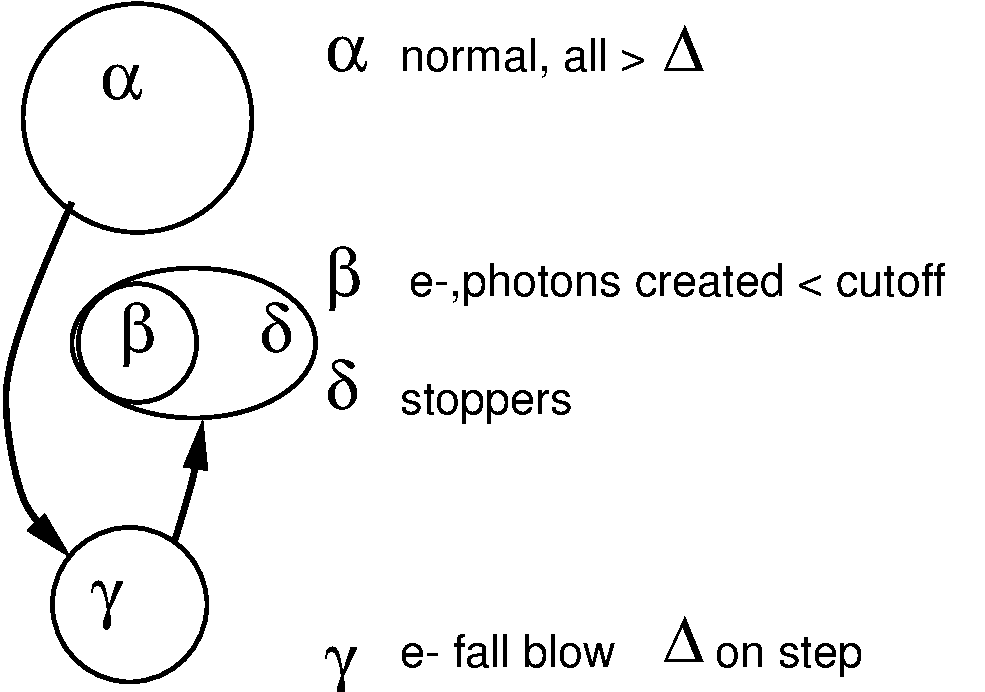
\includegraphics[height=5cm]{figures/sprrz_logic}
\end{center}
\caption[Energy deposition classes in SPRRZnrc]{Modes of energy deposition considered in SPRRZnrc. $\alpha$ events
are those in which energy is deposited by electrons in a step with the
energy entirely above $\Delta$. $\gamma$ events are those in which the
electron starts a step with its energy greater than $\Delta$ and ends with
an energy below $\Delta$. The $\delta$ events are all those events in which
an electron or photon are being terminated because they are below the
cutoffs AE or AP.  This includes a subset of $\beta$ events formed by
electrons and photons which are created with their energy initially below
AE or AP.}
\label{fig_spr_logic}
\end{figure}

The dose delivered by the $\alpha$ events in figure~\ref{fig_spr_logic}
is simple to analyze. In the numerator we just sum the actual energy
deposition. In the denominator we sum the energy deposition times
the ratio of restricted stopping powers at the mid-point energy of the
step, i.e.
\eqn{EDEP \frac{\rspE{Emid}{g}}{\rspE{Emid}{m}}}
This gives how much energy would be deposited in medium $g$ instead of
medium $m$.

The $\beta$ events are not scored at all, except in an evaluation of the
total dose. These events correspond to electrons or photons being created
in the cavity region below the respective transport cut-offs. It is
arguable how to deal with these events, but in traditional calculations
starting from electron spectra they were either ignored or lumped in with
the stoppers.  This issue has been discussed in Borg et al, and there is no
clear solution at this time\cite{Bo99a}.  However, the fraction of the dose contributed
in the cavity region from these events is output by SPRRZnrc and found to
be very small for electron beams or for photon beams at \Co~ energies and
higher. This fact makes the problem academic in most situations.  The
problem becomes serious for low-energy photon beams, but here the
application of Spencer-Attix cavity theory is also suspect\cite{Bo99a}.

The $\delta$ or stopper events which are not $\beta$ events,
are scored as part of the track-end term in
eqn(\ref{eq_sa_spr}).  This is done by scoring the natural energy deposition
in the numerator and the same energy deposition multiplied by the ratio of
the unrestricted stopping powers at $\Delta$ (which are equal to the
restricted stopping powers), i.e.:
\eqn{EDEP \frac{\rspt{g}}{\rspt{m}}.}
Note that this does not merely correspond to the energy deposition in the
second medium, because for a stopper, the energy deposition would be the
same in both media (it just deposits all of its energy which is the same in
both cases). The track-end term in eqn(\ref{eq_sa_spr}) is derived to take
into account that the number of stoppers in each medium will differ because
the fluence of particles stopping in each medium will differ and this
number of stoppers is proportional to the stopping power.

The $\gamma$ events, those particles which cross $\Delta$ during their step
are scored by treating the step as having two components.  The component
with energy above $\Delta$ is treated as if it were an $\alpha$ event and
the component of the energy deposited below $\Delta$ is treated as a
$\delta$ event.

\begin{table}[htb]
\begin{center}
\caption{Energy deposition classes and their components}
\begin{tabular}{|cc|}
\hline
IT value & included events \\
\hline
1  & $\alpha + \gamma + (\delta -\beta)$ \\
3  & $\alpha + \gamma$\\
total & $\alpha + \gamma + \delta$ \\
\hline
\end{tabular}
\end{center}
\end{table}
The SPRRZnrc program scores 3 different doses: the total dose;
dose including everything except the
$\beta$ component (stoppers created below $\Delta$)[IT=1]; dose from
$\alpha$ plus $\gamma$ only [IT=3].
The IT=2 and IT=4 components
correspond to the IT=1 and IT=3 components but scored in the $g$ material
as outlined above. The code then outputs: the total dose; the
fraction of the total dose due to included stoppers (IT=1~$-$~IT=3)/total;
and the fraction of the total dose due to excluded stoppers
(total$-$~IT=1)/total.

The IT=2 dose component is the same as the IT=1 dose component except as
modified to represent the dose in the detector medium as described above.
The IT=4 component similarly corresponds to the IT=3 component, i.e. the
dose less the actual stoppers but including the crossers.

The stopping-power ratios are calculated as the IT=1 dose component divided
by the IT=2 dose component (strictly the scored energy depositions divided
by the respective densities are used).  The stopping-power ratio less the
stoppers is calculated by taking IT=3 divided by IT=4.

The code outputs he two different stopping-power ratios to demonstrate that
the inclusion of the stoppers has only a small effect on the overall
stopping-power ratio, which is a good thing since the treatment of the
stoppers is somewhat arbitrary.  However, it should be pointed out that the
$\gamma$ events are not classified as stoppers but in fact they do contain
some element of the stoppers dose since steps are not stopped at $\Delta$,
but rather at some energy slightly less than $\Delta$.



%\clearpage











\subsection{Input/output control}
\index{SPRRZnrc!I/O control}

I/O control input is delimited between \verb+:start I/O control:+\\
and \verb+:stop I/O control:+.  Most I/O control input
for SPRRZnrc is common to all user codes and is described in
section~\ref{common_I_O_control}\lpage{common_I_O_control}.  However,
the {\tt SPR OUTPUT} control is unique to SPRRZnrc and you input it
as follows:
\begin{verbatim}
  SPR OUTPUT
        = regions         (0)  Specify stopping power ratio output by
                               regions (no .plotdat file will be generated)
        = slabs/cylinders (1)  Specify stopping power ratio output by slabs
                               & cylinders (.plotdat file is generated)
***************************************************************************

  IF SPR OUTPUT= regions

  SPR START REGION   (M)  region numbers in which to start scoring stopping
                           power ratios

  SPR STOP REGION    (M)  region numbers in which to stop scoring stopping
                           power ratios

***************************************************************************

  IF SPR OUTPUT= slabs/cylinders

  SPR IN CYLINDER IX  (M)  Cylinder numbers for which to output
                           stopping power ratios (= 0 for no output)

  SPR IN SLAB IZ      (M)  planar slab numbers for which to output
                           stopping power ratios (= 0 for no output)

**************************************************************************
\end{verbatim}
\index{.plotdat!SPRRZnrc}

\subsubsection{{\tt SPR OUTPUT} options}
\index{SPRRZnrc!SPR OUTPUT}

\index{range rejection!SPRRZnrc}
{\tt SPR OUTPUT} is used to determine how stopping power ratios are
output.  If electron range rejection is off, then stopping power ratios
in all regions are output to the {\tt .egslst} file.  If electron
range rejection is on, then stopping power ratios are zeroed in the
{\tt .egslst} file except in regions specified using
{\tt SPR START REGION} and {\tt SPR STOP REGION} (if
{\tt SPR OUTPUT= regions}) or in slabs/cylinders specified using
{\tt SPR IN CYLINDER IX} and {\tt SPR IN SLAB IZ} (if
{\tt SPR OUTPUT= slabs/cylinders}).  In addition, electron range rejection
is automatically turned off in the regions/slabs/cylinders you have selected
for output so that the stopping power ratios will be meaningful.  If you
are using the {\tt SPR OUTPUT= slabs/cylinders} option, then you will also
get a {\tt inputfile\_dd.plotdat} file which contains the stopping power ratios (and
doses) in the selected slabs and a {\tt inputfile\_rad.plotdat} file
containing stopping power ratios (and doses) in the selected cylinders.
This files are in a format that can be plotted
with {\tt xmgrace} or other plotting program.
\index{.plotdat!SPRRZnrc}

\subsection{Monte Carlo control}
\index{SPRRZnrc!Monte Carlo control}

Monte Carlo control input is delimited between
\verb+:start Monte Carlo inputs:+\\
and \verb+:stop Monte Carlo inputs:+. In addition to the Monte Carlo inputs
common to all user codes (see section~\ref{MC_inputs}\lpage{MC_inputs}),
SPRRZnrc has the following Monte Carlo input:
\begin{verbatim}
  PHOTON REGENERATION         (C)  yes => primary photons are regenerated
                                          after they interact and scattered
                                          photons are thrown away.
                                   no (default) => full calculation

\end{verbatim}
\index{photon regeneration!SPRRZnrc}

\subsubsection{{\tt PHOTON REGENERATION} option}
\index{SPRRZnrc!photon regeneration}
\label{photregsect}

The photon regeneration option is used to calculate the stopping power ratios
for electrons resulting from an unattenuated and unscattered photon beam.
If {\tt PHOTON REGENERATION= yes}, then, prior to a pair production,
compton, photoelectric or Rayleigh event, the properties of the photon about
to interact are saved.  After the interaction, any scattered photons or
photons resulting from relaxation process are discarded and (once all
secondary electrons have been transported) transport reverts to the duplicate
photon that was saved just before the interaction.  In addition, photons
resulting from bremsstrahlung events and positron annihilation events are
eliminated on the spot.
%, and positrons resulting from pair events are
%converted to electrons.
%\note{Why are positrons made into electrons in photon regeneration?}
%\note{Same occurs in general? WHY?????}

This option is to be used when calculating stopping-power ratios for use
in air kerma cavity ion chamber standards since the basic theory makes this
assumption. This makes the calculated stopping-power ratio independent of
the details of the geometry as long as there is full buildup.  This is
discussed in detail by Borg et al\cite{Bo99a}.  This option should not be
used when calculating stopping-power ratios in a phantom since in that case
you want the effects of scatter and attenuation to be taken into effect.


%\renewcommand{\rightmark}{{CAVRZnrc}}
%%%%%%%%%%%%%%%%%%%%%%%%%%%%%%%%%%%%%%%%%%%%%%%%%%%%%%%%%%%%%%%%%%%%%%%%%%%
\section{CAVRZnrc}
%%%%%%%%%%%%%%%%%%%%%%%%%%%%%%%%%%%%%%%%%%%%%%%%%%%%%%%%%%%%%%%%%%%%%%%%%%%
\renewcommand{\leftmark}{{CAVRZnrc}}
\index{CAVRZnrc}

\subsection{Introduction}

CAVRZnrc calculates various factors of interest when using cavity ion
chambers such as $A_{att}$ and $A_{scat}$ and $A_{wall}$.
It has been described in detail in various
publications\cite{Bi85,Ro85a,RB90a,Bi90a} and shown to produce results in
good agreement with standard theory\cite{Bo99a}.

\subsection{Cavity inputs}
\index{CAVRZnrc!cavity inputs}

CAVRZnrc requires an extra set of
inputs defining the cavity region.  These inputs must appear between the
delimiters {\tt :start cavity inputs:} and {\tt :stop cavity inputs:}.

If the user has input the radial geometry using
{\tt METHOD OF INPUT= individual} or {\tt METHOD OF INPUT= groups}
(see section~\ref{geomsect}\lpage{geomsect}), then the following inputs must
appear between the cavity input delimiters:
\begin{verbatim}
   NUMBER OF CAVITY REGIONS (I)   number of geometrical zoneS
                                  comprising the cavity.

   REGION NUMBERS OF THE CAVITY  (M)
                                  the array of these zones
                                  (the cavity region numbers)
\end{verbatim}
Thus, the user defines the cavity in terms of region numbers within the
geometry.

Alternatively, CAVRZnrc offers another method for entering the geometry
in which the geometry is
automatically defined based on cavity information specified by the user.
In this case, only {\tt METHOD OF INPUT= cavity information} needs to be
entered between the {\tt :start geometrical inputs:} and
{\tt :stop geometrical inputs:} delimiters.  Then, between the
cavity input delimiters, the following inputs must be supplied:

\begin{verbatim}

   WALL THICKNESS      (R)   thickness of the chamber walls (cms)
                             (defaults to 0.273)

   CAVITY RADIUS       (R)   outer radius of the cavity (cms)

   CAVITY LENGTH       (R)   length of the cavity (cms) (defaults to 0.2)

   ELECTRODE RADIUS    (R)   radius of the electrode (defaults to 0.)

   WALL MATERIAL       (C)   wall material

   only if   ELECTRODE RADIUS > 0.0
   ELECTRODE MATERIAL  (C)   electrode material
\end{verbatim}
CAVRZnrc creates a simple 3-cylinder
({\tt RCYL(1)=ELECTRODE RADIUS, RCYL(2)=\\CAVITY RADIUS, RCYL(3)=
CAVITY RADIUS + WALL THICKNESS}), 3-slab ({\tt ZPLANE(1)=0,\\
ZPLANE(2)=WALL THICKNESS, ZPLANE(3)=WALL THICKNESS + CAVITY LENGTH,\\
ZPLANE(4)=2*WALL THICKNESS + CAVITY LENGTH}) geometry based on these
inputs.  The material in the cavity is assumed to be AIR.  This option was
useful for early calculations but is not adequate for chambers in which we
want to include much detail.

\subsection{Input/output control}
\index{CAVRZnrc!I/O control}
\label{cavrziosect}

As with the other user codes, I/O control inputs must appear within
the delimiters {\tt :start I/O control:} and {\tt :stop I/O control:}.
In addition to I/O controls that are common to all user codes (see
section~\ref{common_I_O_control}\lpage{common_I_O_control}), CAVRZnrc
has the following inputs:
\begin{verbatim}
  STORE INITIAL RANDOM NUMBERS
        = no          (0)  do not store initial random numbers
        = last        (1)  store initial random number for last history
        = all deposited (2)store the initial random number for all
                           that deposit energy in the cavity
        = all         (3)  store all the initial random numbers

  OUTPUT OPTIONS
        = short              (0)  short output -just the cavity summary
                                  and the dose grid.
        = cavity details     (1)  above plus details for each cavity zone
\end{verbatim}
\index{CAVRZnrc!store initial random numbers}
The {\tt STORE INITIAL RANDOM NUMBERS} input has been included here because
CAVRZnrc has one option, {\tt STORE INITIAL RANDOM NUMBERS= all deposited},
that is not included in the other user codes (see
section~\ref{rnssect}\lpage{rnssect}).
With this option, the initial random numbers from only those histories that
end up depositing energy in the cavity region are stored in the
{\tt .egsrns} file.  Then, if the run is restarted with
{\tt IRESTART= start-RNS} (see section~\ref{restartsect}\lpage{restartsect}),
all histories will end up depositing energy in the cavity region.

\index{CAVRZnrc!output options}
If the user chooses {\tt OUTPUT OPTIONS= short}, then dose and correction
factors will only be output for the cavity as a whole.  If
{\tt OUTPUT OPTIONS= cavity details}, then dose and correction factors
will be output for the cavity as a whole and for each region that makes up
the cavity.

\subsection{Monte Carlo control}
\index{CAVRZnrc!Monte Carlo control}

Monte Carlo control input is delimited between
\verb+:start Monte Carlo inputs:+\\
and \verb+:stop Monte Carlo inputs:+.  In addition to Monte Carlo inputs that
are common to all user codes (see
section~\ref{MC_inputs}\lpage{MC_inputs}), CAVRZnrc had the following
Monte Carlo inputs:
\begin{verbatim}
  IFULL
         = dose and stoppers     (0) just calculate total dose
         = Aatt and Ascat        (1) Above plus Aatt, Ascat
         = Ap                    (2) Above plus Ap as well (option
                                     currently disabled)
         = Afl and <s>g/w        (3) Above plus Afl and <s>g,w as well
                                     (option currently disabled)

  STATISTICAL ACCURACY SOUGHT    (R) % statistical accuracy of the total
                                     dose in the peak region that is
                                     sought The program executes until this
                                     accuracy is obtained or the CPU time
                                     runs out.
  PHOTON REGENERATION
         = yes (1) the calculation is performed with regeneration
                           of the parent photon after they have
                           interacted. A typical setting when FANO
                           conditions are examined.
         = no (0)  a normal calculation.
         = no electrons from wall (ifano = 2) secondary electrons from
                           interactions in the cavity wall are immediately
                           eliminated.  Photons are not regenerated.
                           [IFANO]
\end{verbatim}
\index{photon regeneration!CAVRZnrc}

\subsubsection{{\tt IFULL= dose and stoppers} option}
\index{CAVRZnrc!IFULL}
\index{CAVRZnrc!output of dose}
\label{cavrzifullsect1}

If {\tt IFULL= dose and stoppers}, then CAVRZnrc will output the total
dose in the cavity and, if {\tt OUTPUT OPTIONS= cavity details},
in each region making up the cavity to the {\tt .egslst} file.

\subsubsection{{\tt IFULL= Aatt and Ascat} option}
\index{CAVRZnrc!output of $A_{att}$ and $A_{scat}$}
\label{cavrzifullsect2}

The methods used to calculate the various correction factors have been
described in the literature\cite{Bi85,Ro85a,Bi86,RB90a}.
%\note{This section on Awall needs to be completed .}

If {\tt IFULL= Aatt and Ascat}, then CAVRZnrc will output the total dose,
$A_{att}$, $A_{scat}$ and $A_{wall}$ in the cavity and, if {\tt OUTPUT
OPTIONS= cavity details}, in each region of the cavity to the {\tt
.egslst} file. The listing files also include $K_{wall} = 1./A_{wall}$
(etc).

The scatter correction factor, A$_{scat}$, is defined as the ratio of the
total energy deposited in the cavity to the energy deposited by electrons
generated by primary photon interactions~\cite{Bi86}.  In CAVRZnrc,
photons are flagged as secondary if they have been scattered in compton,
or Rayleigh events, generated by bremsstrahlung or positron annihilation
events, generated by atomic relaxations after compton or photoelectric
events, or if their energy is deposited locally because they have
energy $<$ N-shell energy in a photoelectric event.  Once CAVRZnrc has
totalled the energy deposited in the cavity by electrons generated by
primary photons (ECAV$_{prim}$), and the energy deposited in the cavity
by electrons generated by photons flagged as secondary (ECAV$_{sec}$),
A$_{scat}$ is calculated using the equation:

\begin{equation}
A_{scat}=1+\frac{ECAV_{sec}}{ECAV_{prim}}
\end{equation}

\subsubsection{{\tt STATISTICAL ACCURACY SOUGHT}}
\index{CAVRZnrc!statistical accuracy sought}

If you input a value for {\tt STATISTICAL ACCURACY SOUGHT}
other than zero, then CAVRZnrc will stop when the percent uncertainty on the
total dose in the cavity volume (all cavity regions combined) is equal
to {\tt STATISTICAL ACCURACY SOUGHT} provided that
{\tt NUMBER OF HISTORIES} (see section~\ref{histsect}\lpage{histsect})
or {\tt MAX CPU HOURS ALLOWED} (see section~\ref{cpusect} \lpage{cpusect}) have
not been reached first.

\subsubsection{{\tt PHOTON REGENERATION} options}
\index{photon regeneration!CAVRZnrc}

CAVRZnrc offers two photon regeneration options.  If the user selects
{\tt PHOTON REGENERATION= yes}, then photon regeneration is similar to
that in SPRRZnrc (see section~\ref{photregsect}\lpage{photregsect}).
Unlike SPRRZnrc, where it is required for proper
stopping power ratio calculations as used in primary
air-kerma standards, the purpose of this option in CAVRZnrc is
mainly for theoretical benchmark calculations ({\em e.g} testing
for artefacts under Fano conditions). An additional use
could be for an independent verification of $A_{wall}$: one
runs simulations with {\tt PHOTON REGENERATION= ON} and {\tt PHOTON
REGENERATION= OFF}, the
ratio of the two doses is per definition $A_{wall}$. This is
however not very efficient and a better way to accomplish
this task is to use the cross section enhancement or
photon splitting options described below.

The second regeneration option in CAVRZnrc is {\tt PHOTON REGENERATION= no
electrons from wall}.  With this option, charged particles resulting from
pair production, compton and photoelectric events are eliminated provided
that the interaction did not take place inside the cavity.
This is a hack that has been used to study
the dose fraction from photon interactions in the cavity.

\subsection{CAVRZnrc variance reduction techniques}

\subsubsection{Photon cross section enhancement}
\label{cavrz_cse}
\index{cross section enhancement!CAVRZnrc}
\index{CAVRZnrc!cross section enhancement}

The cross section enhancement technique in CAVRZnrc is
similar to the one implemented in DOSRZnrc
(see section \ref{dosrz_cse} page~\pageref{dosrz_cse}) but
in CAVRZnrc it is applied globally in the entire geometry and the value of
$C_e$ is input directly (as opposed to C as input in the DOSRZnrc case).
Cross section enhancement in CAVRZnrc can be turned on by
including the following line in the input file:
\begin{verbatim}

  CS ENHANCEMENT FACTOR=  some real number [cs_enhance]

\end{verbatim}
If the input is missing or less than unity, there will be
no effect.  But if the enhancement factor is set to greater than unity, the
effect is dramatic: all other user input concerning photon forcing,
splitting, exponential transform, etc., is ignored. In addition,
the calculation result \underline{always} corresponds
to the {\tt IFULL= Aatt and Ascat} option, no matter what the
user requested (but only $A_{wall}$ is calculated,
not the individual $A_{scat}$ and $A_{att}$, see
section \ref{cavrzifullsect2}). In addition, all scoring
is done using proper history-by-history statistics using
the common block {\tt score1}.  The drawback is that dose
and $A_{wall}$ are calculated for the whole cavity and
not on a region-by-region basis as under normal
CAVRZnrc operation.

The following text gives a brief description of the differences
to the DOSRZnrc implementation: The motivation behind the
implementation of cross section enhancement in CAVRZnrc was the desire to
have an independent calculation technique for $A_{wall}$ that is
not too inefficient compared to the unweighting technique. Indeed,
$A_{wall}$ can be calculated by running two separate CAVRZnrc
simulations, one with normal transport  and one with attenuation
and scatter removed via the {\tt photon regeneration= on} option. The ratio of the
cavity dose from the former to the dose from the latter calculation is by
definition $A_{wall}$. Because both calculations
are uncorrelated, their uncertainties add in quadrature and so, the uncertainty
on $A_{wall}$ is larger than the individual dose uncertainties.
The purpose of the cross section enhancement implementation in
CAVRZnrc is to make the two necessary dose calculations at once
and thus reduce the uncertainty of $A_{wall}$ because of the strong
correlation between the ``normal'' dose and the dose with
attenuation and scatter removed. To accomplish this task,
scattered photons are killed as in DOSRZnrc with probability
$1/C_e$. If they survive, they are marked as scattered by setting
their {\tt latch} variable to 3. Unlike in DOSRZnrc, the unscattered
portion of primary photons is always kept on the stack and transported.
However, these non-scattered fractions of primary photons are marked
as attenuated primary photons ({\tt latch=2}) with probability
$1-1/C_e$ and therefore their descendents only contribute to the
dose with attenuation and scatter removed. In addition, scatter,
bremsstrahlung and annihilation from {\tt latch=2} particles are
immediately removed from the stack. It is then clear that
{\tt latch=0,2} electrons contribute to the dose with
attenuation and scatter removed, {\tt latch=0,3} electrons to
the normal dose.

\subsubsection{Photon splitting}
\index{photon splitting!CAVRZnrc}
\index{CAVRZnrc!photon splitting}
\label{cavrzsplitsect}

An additional variance reduction scheme offered in CAVRZnrc
is the photon splitting technique.
Input that turns on photon splitting must appear
between the {\tt :start variance reduction:}
and {\tt :stop variance reduction:} delimiters and is:

\begin{verbatim}

 PHOTON SPLITTING=    (I)    Number of times to split a photon
                             If missing or < 2  => normal transport
                             If >= 2 (allowed only for ifull= dose and
                             stoppers or = Aatt and Ascat), the macro
                             $SELECT-PHOTON-MFP essentially replaces the
                             entire PHOTON routine.
                             [n_split]

\end{verbatim}

This technique is borrowed from Ref. \cite{KF99} where it was shown
to increase the efficiency of external photon beam calculations for
radiotherapy by up to a factor of 5. The increase in CAVRZnrc is
not so dramatic, nevertheless an increase in the efficiency
of cavity dose calculations of up to a factor of 3 compared to using photon
forcing has been observed.

This option is only available with {\tt IFULL= dose and stoppers or =Aatt and Ascat}.
It is also possible to use the {\tt ifano} option (only
if {\tt IFULL=0}). Note that with photon splitting
on, all scoring
is done using proper history-by-history statistics using
the common block {\tt score1}.  The drawback is that dose
(and $A_{wall}$ if requested) are calculated for the whole scoring cavity and
not on a region-by-region basis as under normal CAVRZnrc operation.

The algorithm works as follows:
each photon that is to be transported is split into
{\tt n\_split} photons with weights $w_0/${\tt n\_split}
($w_0$ is the original photon weight). The number of
mean-free-paths $\lambda_i$ to the next interaction of the $i$'th
such photon is sampled from
\begin{equation}
\lambda_i = -\ln \left[1 - {\xi + i - 1 \over {\tt n\_split} } \right]
\end{equation}
where $i$ runs from 1 to {\tt n\_split} and where $\xi$ is a random
number. This forces a uniform distribution of interaction sites.
In addition we have $\lambda_{i+1} > \lambda_i$ and therefore
only transport from $\lambda_i$ to $\lambda_{i+1}$ is needed to
get to the interaction site of the $i+1$'st photon from the
interaction site of the $i$'th photon. When one of the split-photons
interacts, all resulting scattered photons are killed with probability
1/{\tt n\_split} and marked as scattered if they survive
({\tt latch=3}). If {\tt IFULL= Aatt and Ascat} or {\tt photon
regeneration= on}, the original photon is
re-created at each interaction site with probability
1/{\tt n\_split} and marked as a regenerated photon ({\tt latch=2}).
As for the cross section enhancement technique, {\tt latch=0,3} particles
contribute to the normal dose, {\tt latch=0,2} particles to the dose
with attenuation and scatter removed. The ratio of the two is
$A_{wall}$ and so, photon splitting is a third independent
technique for calculating this quantity.

A rule of thumb for good efficiency is to use
\eqn{n\_split \ge \frac{N_o}{1. - e^{-\lambda}} }
where $\lambda$ is approximately the number of photon mean free paths in the
geometry of interest and $N_o \ge 5$. For $^{60}$Co, $\lambda$ is about
0.06 for 1 g/cm$^2$ of graphite and so $n\_split$ should be $\ge 80$.

%%%%%%%%%%%%%%%%%%%%%%%%%%%%%%%%%%%%%%%%%%%%%%%%%%%%%%%%%%%%%%%%%%%%%%%%%%%%%
\section{Spherical user codes}
%%%%%%%%%%%%%%%%%%%%%%%%%%%%%%%%%%%%%%%%%%%%%%%%%%%%%%%%%%%%%%%%%%%%%%%%%%%%%

\subsection{Introduction}

Since 2003, the EGSnrc distribution includes a pair of spherical
geometry user codes.
CAVSPHnrc is the spherical analogue of CAVRZnrc, designed for ion chamber
calculations, and has been used extensively for this purpose (see, \eg,
references\cite{Bi90b,RT99}). The other code, EDKnrc, was derived from
SCASPH, an EGS4 user code for the calculation of mono-energetic energy
deposition kernels\cite{Ma88}. EDKnrc has been extended to allow the use
of both monoenergetic and polyenergetic sources.

Both user codes share most of the common features of the RZ user codes
excluding geometry and source types. We will describe these two in the
following subsections and the user is refered to section \ref{Common}
for information on the common input blocks of these codes.

\subsection{Geometry and Material Inputs}

\subsubsection{Geometrical input: spheres and cones}

The geometrical regions subtended by concentric spheres and cones
originating at the common center of the spheres are shown in figure
\ref{fig_spherical}. NR represents the number of spheres and NC the
number of cones. In what follows we explain the input specification of
the geometry.


\begin{figure}[hbt]
\htmlimage{scale=1.2}{}
\begin{center}
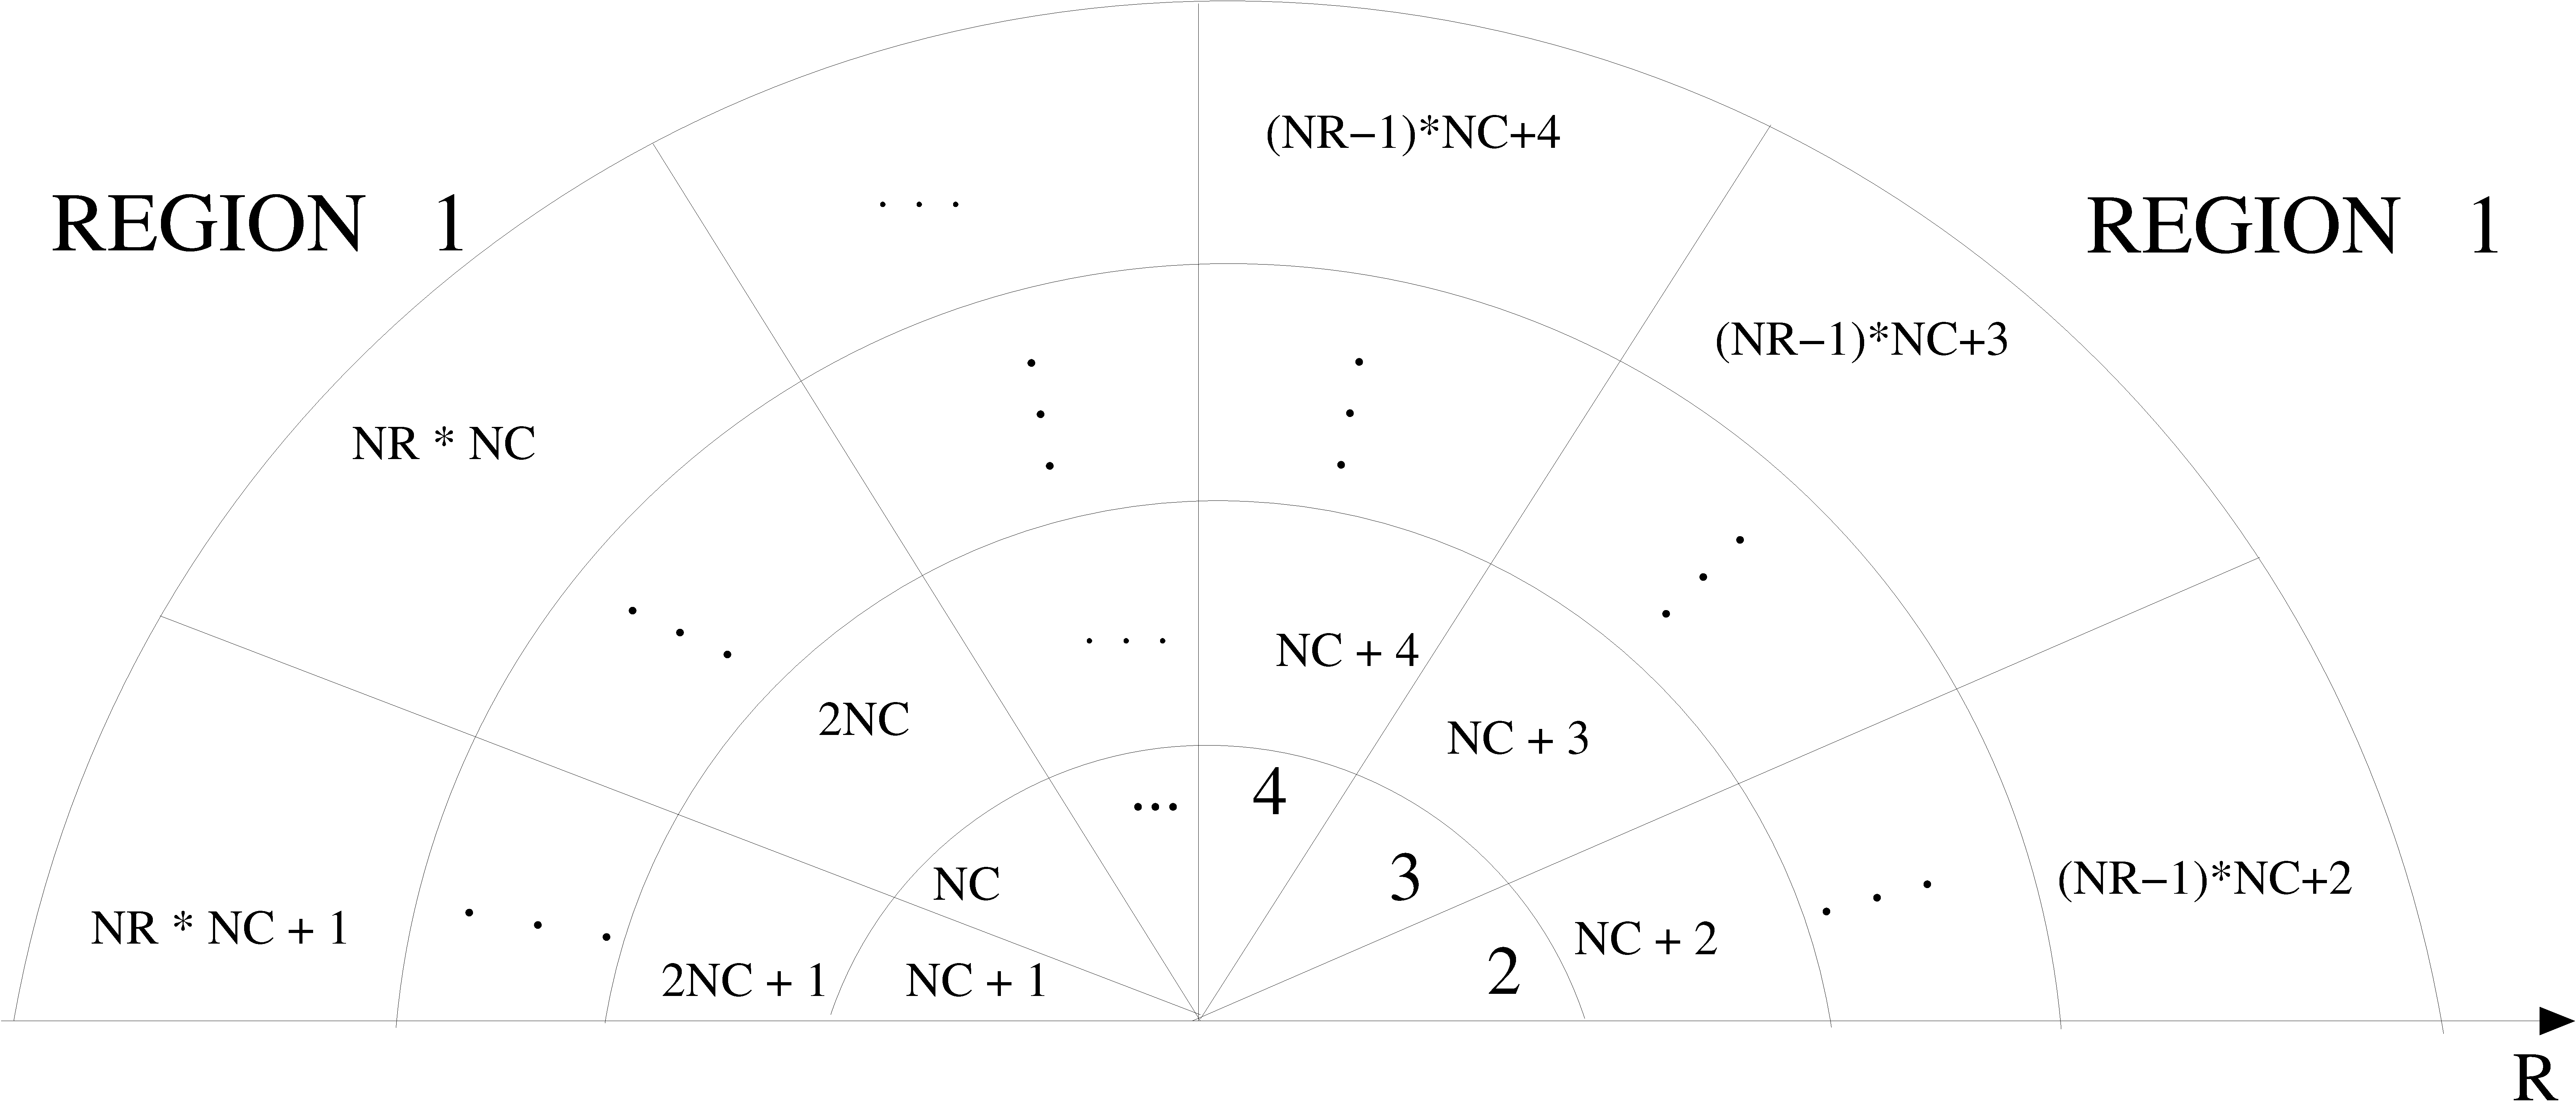
\includegraphics[height=5cm]{figures/spherical}
\end{center}
\caption[Spherical geometry]{Region numbering scheme for the spherical
user codes.  Region number 1 is always outside the geometry. The first
region (2) is defined by the innermost sphere and the cone with the
smallest opening angle. {\tt NR} is the number of radial zones = \# radii
and {\tt NC} = number of cones (0 for purely spherical geometry). }
\label{fig_spherical}
\end{figure}

As in the RZ codes, the geometry inputs are delimited by the strings
{\tt :start geometrical inputs:} and {\tt:stop geometrical inputs:}. The
meaning of the inputs depends on the entries for {\tt NUMBER OF CONES}  and
{\tt NUMBER OF SPHERES}. If a single value is input, then the user is
expected to input the individual corresponding radii or angles. If multiple
values are given for {\tt NUMBER OF CONES}  and/or {\tt NUMBER OF SPHERES},
the user is expected to put in groups of equal angles and/or radii.
If, for instance, several
entries are made for the number of angles, \ie, {\tt NANG1, NANG2, ...}, it
is assumed that the first {\tt NANG1} cones will have the same opening angle
and so on. For spheres, if the user omits the number of radii, it is
assumed that individual entries will be made (after all,
these are user-codes for spherical problems).

\begin{verbatim}
 NUMBER OF CONES= [NANG(1)[,NANG(2),...,NANG(K)]]
                  # If omitted or ZERO, pure spherical geometry assumed
 NUMBER OF SPHERES= [NRAD(1)[,NRAD(2),...NRAD(J)]]
                  # no needed for individual input
\end{verbatim}

Once the user has defined the number of spheres and cones in the problem, the
actual values for the radii and angles must be entered, using the keywords
outlined below:

\begin{verbatim}
RADII= RAD(1), RAD(2), ...RAD(j)
                  #radii of spheres defining the geometry
                  #For group input there must be as many entries
                  #as for the NUMBER OF SPHERES, i.e. :
                  #         J = j
                  #For individual input, NRAD(1) must be equal
                  #to the number of entries, i.e.:
                  #        NRAD(1) = j
                  #unless NUMBER OF SPHERES is omitted, in which case
                  #indiviual input is automatically assumed.
ANGLES= ANG(1), ANG(2),...,ANG(3)
                  #The same rules apply for angles as for radii apply.
\end{verbatim}

One can also enter a group of regions to be considered as the cavity
of a spherical ion chamber and the total dose in these regions will
be computed. For CAVSPHnrc, quantities such as
$K_{att}$ and $K_{scat}$ and $K_{wall}$ are also calculated for the
whole cavity. The specification for the cavity inputs is:
\begin{verbatim}
CAVITY ZONES= [REG1[, REG2...,REGn]] #geometrical zones defined as the
                                     #cavity (real numbers)
\end{verbatim}

\subsubsection{Material input.}

These codes have a simple structure for entering the material input. First
the user must provide a list of media in the problem where the first
medium is taken as default, \ie, every region is considered to have this
medium. Then, medium numbers for all regions where the medium is not
medium 1 must be specified.


\begin{verbatim}
 MEDIA= MEDIUM1, MEDIUM2,..., MEDIUMn

 MEDNUM=        MEDIUM2, MEDIUM2, MEDIUM3,..., MEDIUMn
 START REGION=  START1,  START2,  START3,...,  STARTn
 STOP REGION=   STOP1 ,  STOP2,   STOP3, ...,  STOPn

\end{verbatim}

\subsection{CAVSPHnrc}
The NRC user code CAVSPHnrc (spherical geometry) like CAVRZnrc
(cylindrical geometry) calculates various factors of interest when using
ion chambers such as $K_{att}$, $K_{scat}$, $K_{wall}$ and the dose to the
cavity region per unit incident fluence.

The input file for this user code is very similar to the one for
CAVRZnrc. Only two input blocks are different, the geometry input block
and the input block for the sources. The geometry input was described
previously and the input for the sources differ from CAVRZnrc, in that
only four source types are available: a parallel beam from any angle
(source 0), a point source from any angle (source 1), a parallel beam
from any angle with radial distribution (source 10), a point source from
any angle with radial distribution (source 11).
and a point source from any angle. The source input block is defined by
the delimeters {\tt :start source inputs:} and {\tt :stop source inputs:}
and the same inputs are needed as in CAVRZnrc (see
section~\ref{source_inputs} on page~\pageref{source_inputs}).  In
particular, one must define:

\begin{verbatim}
  INCIDENT PARTICLE= electron   (-1)  electrons
                     photon     (0)   photons
                     positron   (1)   positrons

  SOURCE NUMBER                 (I)   number of the source
                                      [ISOURC]
  SOURCE OPTIONS                (M)   four or five real numbers as specified
                                      below

------------------------------------------------------------------------------

 SOURCE 0/10:  FOR PARALLEL BEAM FROM ANY ANGLE (10-->WITH RAD. DISTN)
              RBEAM,UINC,VINC,WINC
               RBEAM   RADIUS OF THE BEAM AT THE FRONT OF THE TARGET IN CM
                               DEFAULTS TO MAX RADIUS
               UINC    INCIDENT X-AXIS DIRECTION COSINE
               VINC    INCIDENT Y-AXIS DIRECTION COSINE
               WINC    INCIDENT Z-AXIS DIRECTION COSINE
                       NOTE: (UINC,VINC,WINC) GET AUTOMATICALLY NORMALIZED
                             DEFAULTS TO (0.0,0.0,1.0)
------------------------------------------------------------------------------

 SOURCE 1/11:  FOR POINT SOURCE INCIDENT FROM ANY ANGLE (11-->WITH RAD. DISTN)
             DISTR,RBEAM,UINC,VINC,WINC
               DISTR   DISTANCE OF THE SOURCE FROM THE MIDDLE OF THE TARGET
                       IN CM (DEFAULTS TO 100.)
               RBEAM   RADIUS OF THE BEAM AT THE FRONT OF THE TARGET IN CM
                               DEFAULTS TO MAX RADIUS
               UINC    INCIDENT X-AXIS DIRECTION COSINE
               VINC    INCIDENT Y-AXIS DIRECTION COSINE
               WINC    INCIDENT Z-AXIS DIRECTION COSINE
                       NOTE: (UINC,VINC,WINC) GET AUTOMATICALLY NORMALIZED
                             DEFAULTS TO (0.0,0.0,1.0)
------------------------------------------------------------------------------

 SOURCE 10 OR 11:
       SPECIFY MODE:
               MODE = local (0)     IF RADIAL DISTRIBUTION IS TO BE INPUT
                                    LOCALLY WHETHER THROUGH THE KEYBOARD
                                    (INTERACTIVE USE) OR THROUGH THE
                                    .INP FILE (DEFAULT)
                    = external (1)  IF THE DISTRIBUTION IS TO BE INPUT
                                    VIA AN EXTERNAL FILE
       IF MODE=local SPECIFY:

           RDISTF(I)= TOP OF RADIAL BIN I FOR I=1,NBIN
           RPDF(I)= PROBABILITY OF INITIAL PARTICLE BEING IN BIN I FOR
                    I=1,NBIN.

                      PROBABILITIES DO NOT NEED TO BE NORMALIZED
                      BUT SHOULD BE IN UNITS CM**-2

       IF MODE=external SPECIFY:

           RDIST FILNAME = FILENAME(WITH EXT) CONTAINING THE ABOVE INFORMATION


       SPECIFY:
           DISTRIBUTION DATA = NONE => NO DISTRIBUTION DATA IN OUTPUT SUMMARY
                             = OUTPUT SUMMARY => INCLUDE DISTRIBUTION
                               DATA IN OUTPUT SUMMARY
\end{verbatim}

\subsection{EDKnrc}

The NRC user code EDKnrc can be used to calculate Energy Deposition Kernels
for photons or electrons (monoenergetic or polyenergtic) forced to interact
at the centre of a spherical
geometry\cite{Ma05}.  The code can output energy deposition kernels (EDK),
dose distributions in the phantom or the dose to regions defined as the
cavity of a spherical ion chamber.  Voxels are defined by the intersection
of a spherical shell with two cones. See figure \ref{fig_spherical}
for more details.

Although the geometry inputs for this user code are similar to CAVSPHnrc,
there are some major differences in other inputs. The input block for I/O
control, defined by the delimeters {\tt :start I/O control:} and
{\tt:stop I/O control:}, is severely abbreviated.  It includes an entry,
{\tt PRINT OUT EDK FILE} that defines whether energy deposition
kernels will be output in the same format as the ones calculated by
Mackie {\it et al.}\cite{Ma88}. The entire input for this block
is shown below:

\begin{verbatim}

:start I/O control:
  IRESTART
       = first    (0) First run for this data set
       = restart  (1) Restart a previous run
       = analyze  (3) Just read in the raw data and do the statistical analysis
       = parallel (5) Combine results from previous parallel runs
  STORE DATA ARRAYS
       = yes             (0) Store data arrays for re-use
       = no              (1) don't store them
  PRINT OUT EDK FILE
       = yes             (0) EDK stored in old format files
       = no              (1) don't produce EDK files in old format
:stop I/O control:
\end{verbatim}


The input block defining Monte Carlo parameters (delimited by
{\tt start}/{\tt stop Monte Carlo inputs:}) is also abbreviated.  Here
one specifies only the number of histories, the initial random number
seeds, and a variable {\tt IFULL}, which specifies the type of calculation,
and an input specifying whether doppler broadening is to be taken into
account during Compton interactions.

\begin{verbatim}

IFULL= cavity calculation        #(0) calculate dose in cavity regions
     = energy deposition kernels #(1) calculate and output EDK's
     = dose calculation          #(2) calculate and output dose
     = dose and edk              #(3) calculate and output EDK's and dose

DOPPLER BROADENING= On
                  = Off

\end{verbatim}

EDKnrc allows for only three possible sources: 1) a photon source algorithm
that forces photons moving along the Z-axis to interact at the origin
(source 0) 2)
an isotropic point source at the origin for any type of
particle (source 1) 3) same as source 0 but with interaction point shifted
to a user-specified position on the Z-axis (source 2).  Source 2
was left for comparison with older EDK calculations, but the user
is strongly discouraged from using it, since it has been shown to produce
numerical artifacts when computing EDK's. For accurate EDK calculations
source 0 should be used.   The inputs specifying the source type, which is
included within the {\tt start}/{\tt stop Source Inputs:} delimiters,
are shown below:

\begin{verbatim}
SOURCE NUMBER= 0 | 1 | 2
#     0 ==>  Photon moving along Z axis forced to interact at origin
#     1 ==>  Point source at origin, isotropically radiating into 4 Pi
#     2 ==>  Same as 0 but interaction point as in old code

# if SOURCE NUMBER= 2
    ZIN      #-> source offset on Z-axis
             #   Option used to emulate old way of calculating EDK
\end{verbatim}

Note that in the case of source 0 or source 2, the {\tt INCIDENT PARTICLE=}
(standard for all user codes when specifying the source) input must be
set to {\tt PHOTON}.

The energy deposited in the geometry can be separated into different
contributions from each photon scattering order (\eg~ primary,
first scatter, second scatter, multiple scatter and radiative). For
electrons, the deposited energy can be split into primary and radiative
contributions. In the standard output file {\tt *.egslst}, only the total
and primary components are written. ONLY if the user selects the option
for creating old format EDK files, all components are stored to a file
following the convention:
\begin{itemize}
\item {\tt edk[EIN].keV}, for monoenergetic sources,
where EIN is the initial energy in keV.
\item {\tt file\_name.keV}, for polyenergetic sources (spectrum),
where {\tt file\_name} is the standard output file name

\end{itemize}

The user also has the choice to
create xmgrace plot files for the {\bf total dose} by using the input block for plot control delimited by
{\tt :start plot control:} and {\tt:stop plot control:}. A description of this input block is
given below:

\begin{verbatim}
   :start plot control:

   PLOTTING
          = Off         (0)   no plots or plot files to be prepared
          = Histogram   (1)   histogram plotting
          = Point       (2)   xy graph


  ONLY IF not PLOTTING= Off

   PLOT RADIAL REGION IX  (M)  radial regions to plot vs angle
                               (= 0 for no plots)

   PLOT CONICAL REGION IC  (M)  angular intervals to plot vs radius
                               (= 0 for no plots)

   :stop plot control:
\end{verbatim}

Plots in radial regions are written to the file {\tt inputfile.angplot}
({\em i.e.} dose versus angle) and plots in conical regions are written
to the file {\tt inputfile.radplot}.

The output capabilities of this user code are very limited but can be
easily extended to print out all components of the energy deposition
kernels.

\typeout{}
\typeout{***Start of Cited References****}
\typeout{}
\renewcommand{\leftmark}{{REFERENCES}}
\renewcommand{\rightmark}{{REFERENCES}}
\section{References}
\vspace*{-1.7cm}
\bibliography{../irs}
%above points to where we find the master reference list
\typeout{}
\typeout{******REMEMBER to create .bbl  and reset twice**********}
\typeout{}
\bibliographystyle{unsrt}


\newpage
\typeout{**********starting index here******************}
\renewcommand{\leftmark}{{Index}}
\renewcommand{\rightmark}{{Index}}
\addcontentsline{toc}{section}{\numberline{}Index}
\setlength{\baselineskip}{0.5cm}


%%%%%%%%%%%%%%%%%%%%%%%%%%%%%%%%%%%%%%%%%%%%%%%%%%%%%%%%%%%%%%%%%%%%%%%%%%%%%%%
%
%  EGSnrc user codes manual
%  Copyright (C) 2021 National Research Council Canada
%
%  This file is part of EGSnrc.
%
%  EGSnrc is free software: you can redistribute it and/or modify it under
%  the terms of the GNU Affero General Public License as published by the
%  Free Software Foundation, either version 3 of the License, or (at your
%  option) any later version.
%
%  EGSnrc is distributed in the hope that it will be useful, but WITHOUT ANY
%  WARRANTY; without even the implied warranty of MERCHANTABILITY or FITNESS
%  FOR A PARTICULAR PURPOSE.  See the GNU Affero General Public License for
%  more details.
%
%  You should have received a copy of the GNU Affero General Public License
%  along with EGSnrc. If not, see <http://www.gnu.org/licenses/>.
%
%%%%%%%%%%%%%%%%%%%%%%%%%%%%%%%%%%%%%%%%%%%%%%%%%%%%%%%%%%%%%%%%%%%%%%%%%%%%%%%
%
%  Authors:         Dave Rogers
%                   Iwan Kawrakow
%                   Jan Seuntjens
%                   Blake Walters
%                   Ernesto Mainegra-Hing
%
%  Contributors:    Frederic Tessier
%
%%%%%%%%%%%%%%%%%%%%%%%%%%%%%%%%%%%%%%%%%%%%%%%%%%%%%%%%%%%%%%%%%%%%%%%%%%%%%%%


\documentclass[12pt,twoside]{article}  %indexm doesn't work with two
					%sides
%\usepackage{supertab}%this didn't work for some reason?
%\usepackage{overcite}			%comment out for html?

\usepackage{moreverb}	%this is used for the boxedverbatim environment
			%used to box the listing files for tutor programs

\setlength{\textwidth}{16.51cm}
%\setlength{\textheight}{23.2cm}
\setlength{\textheight}{23.5cm}
\setlength{\oddsidemargin}{0.0in}
\setlength{\evensidemargin}{0.0in}
\setlength{\topmargin}{-1.5cm}
\setlength{\parindent}{1.5em}
\setlength{\topsep}{0ex}
\setlength{\itemsep}{0ex}

\newcommand{\lpage}[1]{(page~\pageref{#1})}
\newcommand{\Mol}{Moli\`ere}

\newcommand{\Co}{$^{60}$Co}
\newcommand{\parsp}{~\hspace*{1.5em}}
\setlength{\parskip}{0.1in}
\setlength{\baselineskip}{1.0cm}
\newcommand{\head}[1]{\begin{center}\begin{Large}{\bf #1}
                                              \end{Large}\end{center}}
\newcommand{\cen}[1]{\begin{center} #1 \end{center} }
\newcommand{\etal}{{\em et.al.}}
\newcommand{\ie}{{\em i.e.}}
\newcommand{\etc}{{\em etc.}}
\newcommand{\viz}{{\em viz.}}
\newcommand{\eg}{{\em eg.}}
\newcommand{\sprt}[2]{\left(\frac{\overline{L}}{\rho}\right)^{\rm #1}_{\rm #2}}
\newcommand{\eqn}[1]{\begin{equation} #1 \end{equation} }
\newcommand{\rsp}[1]{\left( \frac{L(\Delta)}{\rho} \right)_{#1}}
\newcommand{\PhiT}{\Phi_{\rm T}}
\newcommand{\rspt}[1]{\left( \frac{S(\Delta)}{\rho} \right)_{#1}}
\newcommand{\rspE}[2]{\left( \frac{L({\rm #1})}{\rho} \right)_{#2}}

\newcommand{\note}[1]{\mbox{}\\ \noindent \rule{16cm}{0.5mm} \\
{\em #1} \\ \noindent \rule{16cm}{0.5mm}\\
\typeout{******note: #1 *****}
}

%\newcommand{\indexm}[1]{\index{#1}}
%\typeout{~~~~~~~~~~~~***margin index feature OFF*****************************}
%\typeout{~~~~~~~~~~~~***margin index feature OFF*****************************}
%\typeout{~~~~~~~~~~~~***margin index feature OFF*****************************}
\newcommand{\indexm}[1]{\marginpar{{\sf {\tiny I:#1} }}\index{#1}}
\makeindex


\renewcommand{\refname}{}

%       some commands to get 4 levels in the table of contents and
%       number down to paragraphs
\setcounter{secnumdepth}{4}
\setcounter{tocdepth}{4}
\renewcommand{\thesubsubsection}{\thesubsection.\arabic{subsubsection}}
\renewcommand{\theparagraph}{\thesubsubsection.\roman{paragraph}}
%\renewcommand{\theequation}{\arabic{subsection}.\arabic{subsubsection}.\arabic{equation}}



%\usepackage{html}
\usepackage{graphicx}
%\usepackage{epsf}
%\input{epsf}
\usepackage{longtable}

\usepackage{fancyhdr}
\renewcommand{\footrulewidth}{0.4pt}
\renewcommand{\headrulewidth}{0.4pt}

\lhead[{\sffamily \thepage}]{{\sffamily NRC User Codes for EGSnrc }}
\rhead[{\sffamily NRCC Report PIRS-702}]{{\sffamily ~\thepage}}
%\rfoot[{\sffamily {\rightmark}}]{{\sffamily {\rightmark}}}
\rfoot[]{{\sffamily {\rightmark}}}
% \lfoot[{\sffamily {\leftmark}}]{{\small Last edited $Date: 2013/09/24 18:04:14 $
\lfoot[{\sffamily {\leftmark}}]{{\small Last edited 2011/05/03 15:50:14
}}
\cfoot{}

\usepackage{hyperref}
\hypersetup{colorlinks=true, citecolor=blue, linkcolor=blue, filecolor=blue, urlcolor=blue}
\urlstyle{same}

\usepackage{html}



\begin{latexonly}
\typeout{***Have turned off overfull and underfull messages****}
\tolerance=10000        %suppress Overfull only
\hbadness=10000         %suppress Overfull and Underfull for text (horizontal)
\vbadness=10000         %suppress Overfull and Underfull for vertical "boxes"
\end{latexonly}


\begin{document}

\begin{htmlonly}
For information about the authors and/or institutions involved with this
work, use the links provided in the author list.\\

\begin{rawhtml}
<br><br>
\end{rawhtml}


Postscript versions of the entire paper are available.  You may have to
download the compressed version to disk, uncompress or gunzip them and
then read or print them.\\
\begin{center}
\htmladdnormallink{(uncompressed version 2.4 Mb)}{pirs702.ps}\\
\htmladdnormallink{(gzip version 230 kb)}{pirs702.ps.gz}\\
\htmladdnormallink{(pdf version 440 kb)}{pirs702.pdf}\\
\end{center}
\begin{rawhtml}
<br><br>
\end{rawhtml}

Use the Up button to get back to this page from within the document.
\begin{rawhtml}
<BR> <HR> <P>
\end{rawhtml}
\copyright
Copyright 2021,  National Research Council of Canada
Ottawa
\begin{rawhtml}
<BR> <HR> <P>
\end{rawhtml}
\end{htmlonly}

\pagestyle{empty}

\title{NRC User Codes for EGSnrc}

\begin{center}
{\sffamily \bfseries {\Huge NRC User Codes for EGSnrc}
\vspace{5mm}\\}
\begin{Large}
D.W.O. Rogers, I. Kawrakow, J.P. Seuntjens,  B.R.B. Walters and E.
Mainegra-Hing \\
\end{Large}
Ionizing Radiation Standards,
National Research Council Canada, Ottawa, Canada\\


\vspace{3mm}
{\bfseries
\today}
%January 2010}
\vspace{3mm}\\
\hfill NRCC Report {\sf PIRS-702(revC)} \vspace*{2mm}\\

\begin{figure}[h]
\htmlimage{scale=1.2}{}
\begin{center}
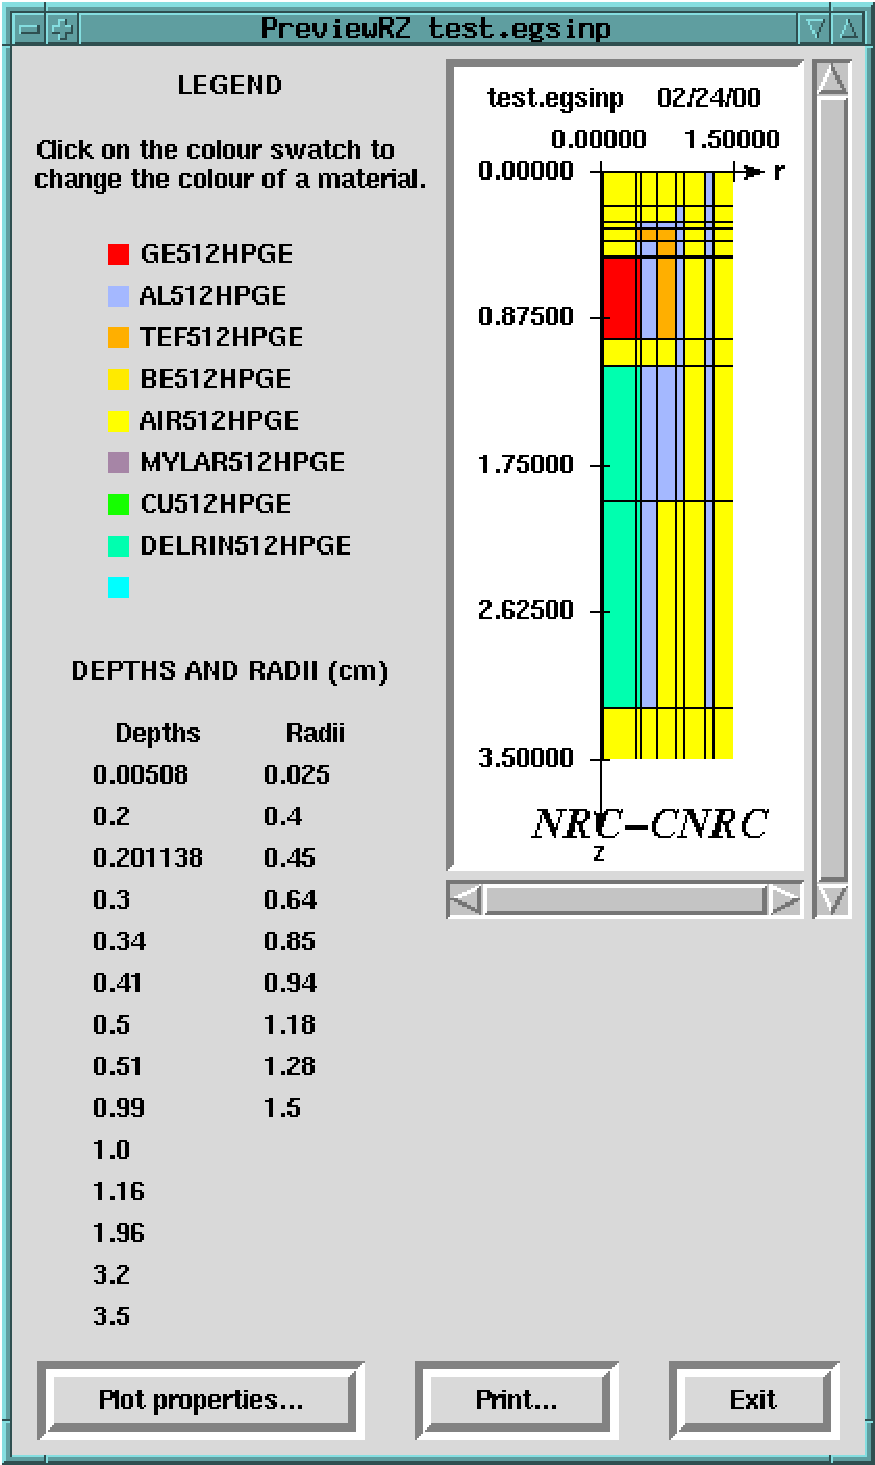
\includegraphics[height=12cm]{figures/PreviewRZ_example}
\\Preview of an RZ geometry in DOSRZnrc.
\end{center}
%\caption{Preview of an RZ geometry in DOSRZnrc.}
%\cen{Get a figure from preview tcl of DOSRZnrc}
\end{figure}

\vfill
\begin{latexonly}
\end{latexonly}

\copyright NRC Canada, 2021
\end{center}
\newpage   %Blank page behind cover
\mbox{}

%\note{This page is intentionally blank to be the back of the front cover.
%Remove this note prior to printing!!!}

\setlength{\baselineskip}{0.5cm}
\newpage

\pagestyle{fancy}
\pagenumbering{arabic}
\setcounter{page}{1}


\begin{abstract}
\label{abstract}
This manual describes the NRC User codes DOSRZnrc, CAVRZnrc, FLURZnrc and
SPRRZnrc which all work with the EGSnrc Code system for Monte Carlo
transport of electrons and photons (see NRC REPORT PIRS--701, ``The EGSnrc
Code System''). There is a graphical user interface available for creating
the inputs to these codes (described separately).

\end{abstract}

%\newpage

\setlength{\baselineskip}{0.1cm}

\tableofcontents

%\newpage
\listoftables
\listoffigures

\setlength{\baselineskip}{0.5cm}

\newpage

\renewcommand{\leftmark}{{INTRODUCTION}}
\section{Introduction}
\subsection{Intent of this report}

Over the years, NRC has developed and distributed a series of user codes
for use with the EGS4 code system for the Monte Carlo simulation of photon
and electron transport.  These have been widely used and their results
compared to experiment in many cases.  However, the codes themselves have
never been properly documented and described. It is the purpose of this
manual to provide a document which describes
both how these codes work and also how a user uses them.  It is not the
purpose of this manual to discuss selection of parameters when using these
codes for a particular application since this is a huge undertaking and is
covered in the already extensive literature on EGS.

Recently, the codes
have been reworked to use the new EGSnrcMP system\cite{Ka03}. This
has increased the flexibility of these codes, including the ability
to run them on both Unix/Linux and Windows systems.

The codes involved in this report are all for
cylindrical RZ and spherical geometries. These are:
\begin{description}

\item[DOSRZnrc] which scores dose in a generalised cylindrical geometry.

\item[FLURZnrc] which scores particle fluence in the same geometry.

\item[CAVRZnrc] which is similar to DOSRZnrc but also scores a variety of
quantities which are of specific interest to dosimetry
calculations for an ion chamber.

\item[SPRRZnrc] which calculates Spencer-Attix spectrum averaged
stopping-power ratios for arbitrary media.

\item[CAVSPHnrc] which is identical to CAVRZnrc but for spherical
geometries.

\item[EDKnrc] which calculates energy deposition kernels for photons
or electrons forced to interact at the centre of a spherical phantom.
It can also calculate dose distributions in the entire phantom or the
dose to specific regions defined as the cavity of a spherical ion chamber.

\end{description}

This manual does not describe the BEAM code for modelling radiotherapy
accelerators, \Co~ units and x-ray systems. BEAM is described
elsewhere\cite{Ro95,Ro98a}. The user codes
described here all have the capability of using either a BEAM generated phase
space file or a full BEAM simulation (compiled as a shared library)
as the source of incident particles.

Also, this manual does not describe the EGS\_Windows system for doing 3D
displays of EGS simulations. EGS\_Windows is described in detail in its own
manual\cite{TR99a}.

\subsection{History}
\index{history}
These codes have a long history at NRC and were first written to work
with EGS3 which was written in Mortran2.  The first germs of these
codes were written by Alex Bielajew who was responsible for coding
CAVRZ as a research tool for work related to ion chamber dosimetry.
This then grew into DOSRZ which strips out some of the special purpose
parts of CAVRZ but adds various more general purpose facilities such as
calculating response functions for detectors. Dave Rogers took these
codes and developed a general purpose fluence scoring code FLURZ and
finally SPRRZ was developed.  Along the way various summer students worked
under Dave Rogers and Alex Bielajew to add features.

One problem was that
all the codes had grown on their own with various bits and pieces being
patched in whenever they were needed for a particular research project.
The system of codes was getting more and more difficult to maintain
and various options failed to work on new systems as they came along
(eg the output listing from FLURZ didn't work on Unix systems
because it was based on a
Digital Vax Fortran extension which was not commonly available on unix
Fortran compilers).  This was overcome in the DOSRZ code by some horrific
coding tricks which made it impossible to change the outputs.  Furthermore the
input files became almost impossible to create since they were just a
large file of numbers where the meaning of each number was dependent on
its position, and often meant different things for the different codes.

To overcome these shortcomings, a major revamping was undertaken in 1998
by Aaron Merovitz, a summer student working for Dave Rogers.  Firstly he
created some general purpose output routines which worked for standard
compilers. Also, as much as possible all graphical output was done through
a single subroutine called {\tt xvgrplot} so that if changes in plotting
output are required. it needs to be changed in only the subroutine.
Next a text based system for input files was written which is much easier
to use than the previously used long string of numbers.  This tool was
then used to create a single routine to read geometry inputs for all the
user codes so that now one can cut and paste the geometry description
from one user code to another. This was extended for source routines and
transport routines so that the input files start to look similar for all
the user codes.  More importantly they are much easier to read and know
exactly what the simulation is about without having the description of
the inputs open on your desk.

In 1999, the codes were upgraded to use the then-new EGSnrc code system.
This was done by Iwan Kawrakow with Jan Seuntjens and Dave Rogers.
In the process many small bugs have been found and fixed.

In 2002, Ernesto Mainegra-Hing developed a very powerful C$++$ graphical
user interface which is based on the Qt(version 3) system\cite{Ma03}.

The final major upgrade has been to make the codes work with the new
EGSnrcMP code system. This has been undertaken by Iwan Kawrakow with
support from Ernesto Mainegra-Hing and Blake Walters.

In the individual descriptions below of the codes we cite various specific
references to papers in which the various aspects of the code have been
described.

As the above history makes clear, these user codes have been developed
by many different people over a long period of time, and the codes
have all benefited by extensive feedback and bug patches from the user
community. In particular, we wish to recognise the contribution of Alex
Bielajew to the development of these codes over a long period of time
while he was at NRC.

\renewcommand{\leftmark}{{COMMON FEATURES}}
\section[Common Features]{Common Features of All Codes and Associated Inputs}
\label{Common}
\subsection{Subroutines in the RZ codes}

\index{subroutines}
As pointed out before, all NRC RZ-codes work within the same RZ
geometry, and their \verb+HOWFAR+ and \verb+HOWNEAR+ routines are
exactly the same. Most of the other common subroutines and macros
have been split off as much as possible (but not completely)
from the user code file. They include:

\begin{itemize}
\item{random number generators (\verb+ranmar.macros+,
\verb+ranmar.mortran+,\\
\verb+ranlux.macros+, \verb+ranlux.mortran+)}
\index{random number generators}

\item{machine specific macros / routines
(\verb+machine.mortran+)}
\index{machine.mortran}

\item{EGSnrc specific macros and routines
(\verb+egsnrc.mortran+, \verb+egsnrc.macros+)}

\item{RZ geometrical subroutines
(\verb+geomrz.mortran+)}
\index{geomrz.mortran}

\item{input parser routines
(\verb+get_inputs.mortran+, {\tt transportp.macros})}
\index{get\_inputs.mortran}
\index{transportp.macros}

\item{Sources and energy sampling routines available for the RZ codes
(\verb+srcrz.mortran+, \verb+ensrc.mortran+, {\tt srcrz.macros},
{\tt phsp\_macros.mortran})}
\index{srcrz.mortran}
\index{srcrz.macros}
\index{ensrc.mortran}
\index{phsp\_macros.mortran}

\item{{\tt IWATCH} output routine
(\verb+nrcaux.mortran+)}
\index{nrcaux.mortran}

\item{Routine to output RZ grid to {\tt .egslst} file ({\tt grids.mortran})}
\index{grids.mortran}

\item{Routines for initializing data I/O, opening output files, etc
({\tt egs\_utilities.mortran})}
\index{egs\_utilities.mortran}

\item{Routines for built-in parallel processing functionality
({\tt egs\_parallel.mortran})}
\index{egs\_parallel.mortran}

\end{itemize}
The scoring routine \verb+AUSGAB+ is fundamentally different for each
of the user codes, and will be discussed later in this document.

\newpage
\subsection{Region and plane numbering convention}
\index{region and plane numbering convention}
\index{numbering conventions}
\index{IX} \index{IZ} \index{NR} \index{NZ} \index{planar regions}
\index{geometry}
\index{axis of rotation}

The numbering of the regions, planar zones and cylindrical
ring zones in the RZ codes is shown in figure~\ref{fig_geom} in which
the Z-axis is the axis of rotation shown by the dotted line running
across the page. \verb+NR+ represents the number of cylinders  or rings, and
\verb+NZ+ the number of planar regions or slabs,
which are defined by {\tt NZ + 1}
planes.
(\verb+IX+,\verb+IZ+) denote the (r,z) indices of a subregion in the
RZ space.
The input specification of the geometry and materials is summarised
in the next section.

\begin{figure}[htb]
\index{region and plane numbering convention}
\index{IX} \index{IZ} \index{NR} \index{NZ} \index{planar regions}
\index{geometry}
\index{axis of rotation}
\begin{center}

%\begin{boxedverbatim}
\begin{verbatim}






      ------------------------------------------------------- RCYL(NR)
      |(NR-1) |(NR-1) |(NR-1) |    . . .    | NR*NZ | NR*NZ |    IX=NR
      | *NZ+2 | *NZ+3 | *NZ+4 |             |       |   +1  |
      ------------------------------------------------------- RCYL(NR-1)
      |   .   |   .   |   .   |             |   .   |   .   |
      |   .   |   .   |   .   |             |   .   |   .   |
      |   .   |   .   |   .   |             |   .   |   .   |
      ------------------------------------------------------- RCYL(2)
      |  NZ+2 |  NZ+3 |  NZ+4 |    . . .    |  2NZ  | 2NZ+1 |    IX=2
      ------------------------------------------------------- RCYL(1)
..1...|...2...|...3...|...4...|.............|...NZ..|..NZ+1.|....IX=1..1..
      -------------------------------------------------------
      |       |       |       |    . . .    |       |       |
      -------------------------------------------------------
      |   .   |   .   |   .   |             |   .   |   .   |
      |   .   |   .   |   .   |             |   .   |   .   |
      |   .   |   .   |   .   |             |   .   |   .   |
      -------------------------------------------------------
      |       |       |       |    . . .    |       |       |
      |       |       |       |             |       |       |
      -------------------------------------------------------
        IZ=1    IZ=2    IZ=3                 IZ=NZ-1  IZ=NZ


\end{verbatim}
%\end{boxedverbatim}
\caption[Schematic of the RZ geometry and notation.]{Geometry of the
RZ NRC user codes.  The dotted line is the z-axis which is the axis
of rotation.  The exterior of the geometry is zone 1.  There are {\tt
NZ} depth slabs or regions which are defined by {\tt NZ + 1} planar boundaries
specified by  {\tt ZBOUND(1:NZ+1)}. There are {\tt NR} radial regions or
rings
defined by their {\tt NR} outer radii contained in {\tt RCYL(1:NR)}. The region
numbers are reflected in the axis of rotation.
\label{fig_geom}
\vspace{3mm} }
\end{center}
\end{figure}


\newpage
\subsection{Using the text based input format}
\label{UNIF}
\index{text based input}
\index{GET\_INPUT}
\index{get\_inputs.mortran}

The input for the RZ codes is handled by each code's
INPUTS subroutine. It in turn makes multiple use of a common routine called
\verb+GET_INPUT+.
The function is located in the file \verb+get_inputs.mortran+
and for the RZ codes it is, along with other files, concatenated before
being compiled.
We briefly describe the use of the function \verb+GET_INPUT+
for implementation in user codes.

\verb+GET_INPUT+ will extract the requested
\verb+values_sought+ from the input file and return it to the
caller. Inputs are all in the format:\\
 \verb+name of value_sought= value+\\
where \verb+name of value_sought+ must match that expected by the
program.  Example of typical inputs handled by \verb+GET_INPUT+ are:
\begin{verbatim}
                MEDNUM= 0, 1, 2
                MEDIA= AIR700ICRU
                RAYLEIGH SCATTERING= on
\end{verbatim}
\index{GET\_INPUT!rules of use}
The rules governing the use of the {\tt GET\_INPUT} routine are:
\begin{itemize}
\item The \verb+value_sought+ must be the first thing on a line but
blanks are allowed before it.

\index{value\_sought}
\index{= in input files}
\item The {\tt =} sign must have no blanks between it and the text for
the \verb+value_sought+ and at least one blank before the value input.

\item Various inputs are only sought between certain delimiter strings
which are defined below ({\em e.g.},
\verb+ :start I/O control: :stop I/O control:+)
If the delimiter string is not specified, the whole file is searched for
a requested \verb+value_sought+.

\index{delimiter strings}
\item Delimiter strings are enclosed by colons.

\item Within delimiter strings, order of inputs does not matter.

\item If a requested quantity is not found, this is noted in the file
\verb+$input.errors+ and this file is printed at the end of the log file.
\index{\$input.errors file}

\item A semi-colon implies the end of input for this quantity but is
not mandatory.  This means that semi-colons cannot be used in titles.
\index{; in input files}

\item A \verb+#+ sign indicates that everything else on the line is a
comment (do not use in titles).
\index{\verb+#+ in input files}

\item Commas separate multiple values for a given quantity and a comma
at the end of a line implies there is more input on the next line.
\index{, in input files}

\item There can be coupled multiple inputs whereby the first value of some
{\tt value\_sought} is associated with the first value of some other {\tt
value\_sought} and possibly with the first value of a third {\tt
value\_sought}, etc.
\index{multiple inputs}

\item Values can extend over as many lines as needed. Use commas to imply
there are more values on the next line.

\item Blank lines and blanks in general are ignored.
\index{blanks in input files}

\item The maximum record length is 256 characters.

\item Inputs are not case sensitive.
\index{case in input files}

\end{itemize}

\subsubsection{Using {\tt GET\_INPUT}}

This section is only of interest to those wanting to modify the user codes
or add a new input.

There are 4 types of inputs defined: type 0, {\tt REAL} numbers; type 1, {\tt
INTEGER}s; type 2,  arbitrary character strings (eg
titles); type3, predefined
character strings, or ``allowed inputs''.

\index{GET\_INPUT}
To implement \verb+GET_INPUT+ one must first establish a set of requested
inputs and then make a call to {\tt get\_input} for one or more inputs
(which are specified by a counter).

The following summaries the implementation of \verb+GET_INPUT+ for
different types of input.
\begin{verbatim}
              REALS AND INTEGERS (TYPE 0 AND 1)
  I=I+1;                              <--index counter
  NUM_DRMIN=I;                        <--named pointer to the index num.
  VALUES_SOUGHT(I)='DOSE RBOUND MIN'; <--name of variable
  NVALUE(I)=1;                        <--# of inputs(left out if not known)
  TYPE(I)=0;                          <--Type (0-3)
  VALUE_MIN(I)=0;                     <--Minimum value
  VALUE_MAX(I)=$MAXRADII-1;           <--Maximum value
  DEFAULT(I)=0;                       <--Default value

              CHARACTER INPUTS (TYPE 2)
  I=I+1;
  NUM_TITLE=I;
  VALUES_SOUGHT(I)='TITLE';
  TYPE(I)=2;
  NVALUE(I)=1;                        <--left out if not known

              ALLOWED INPUTS (TYPE 3)
  I=I+1;
  NUM_IWATCH=I;
  VALUES_SOUGHT(I)='IWATCH';
  NVALUE(I)=1;                        <--left out if not known
  TYPE(I)=3;
  ALLOWED_INPUTS(I,0)='OFF';
  ALLOWED_INPUTS(I,1)='INTERACTIONS';
  ALLOWED_INPUTS(I,2)='STEPS';
  ALLOWED_INPUTS(I,3)='DEPOSITED';
  ALLOWED_INPUTS(I,4)='GRAPH';
                      **** STATE THE DELIMITER ****
            DELIMITER='TRANSPORT CONTROL'
     OR     DELIMITER='NONE';
\end{verbatim}
For REAL and INTEGER input types, the user may specify minimum and
maximum acceptable values, and if the iput is outside this range,
the code uses the specified DEFAULT value. Note however that if the
particular \verb+VALUES_SOUGHT+ is not input, then an error flag is set,
an error message produced and eventually the program in terminated,
i.e. the default value is not a true default.

\index{GET\_INPUT}
After these parameters have been specified, call the subroutine
\verb+GET_INPUT+ with the appropriate index number of the
\verb+values_sought+ (use \verb+NMIN+ and \verb+NMAX+).
An example is shown below.
\begin{verbatim}
    ival=1;
    NUM_ESTEPE=ival;                  --> store index for ESTEPE variable
    VALUES_SOUGHT(IVAL)='ESTEPE';
    NVALUE(IVAL)=1;
    TYPE(IVAL)=1;
    VALUE_MIN(IVAL)=0.0;
    VALUE_MAX(IVAL)=1.0;
    DEFAULT(IVAL)=$MAX-ELOSS;

    IVAL=IVAL+1;
    NUM_XIMAX=IVAL;
    VALUES_SOUGHT(IVAL)='XIMAX';
    NVALUE(IVAL)=1;
    TYPE(IVAL)=1;
    VALUE_MIN(IVAL)=0.0;
    VALUE_MAX(IVAL)=1.0;
    DEFAULT(IVAL)=$EXACT-BCA-XIMAX;

    ...
    NMIN = 1; NMAX = IVAL;            --> specify the range of inputs
    CALL GET_INPUT;                   --> call GET_INPUT

    estepe=VALUE(NUM_ESTEPE,1);       --> assign the variable using
                                          the previously stored index
    ximax=VALUE(NUM_XIMAX,1);
\end{verbatim}

\subsubsection{Note on notation}
The text based input is much clearer than the previous input based on
assigned values to individual variables. The one advantage of the former
system is that the name of the varable used in the source code was made
explicit.  To allow the user to know what the internal variable is called
which is specified by a particular text input, we frequently specify the
name of the associated variable in square brackets after the description of
the text based inputs (eg {\tt [ ECUT ]} and when appropriate, the
internal values corresponding to the different options are shown.
\index{notation}
\index{internal variable names}
\index{variable names}

\subsection{The xmgr/grace plotting codes}
\index{xmgr}
\index{grace}
\index{plotting}
\index{plotxvgr}

At NRC we make extensive use of the freeware, called {\tt xmgr} or more
recently {\tt grace} for making 2-D plots of data.  Most of these user
codes now create files which can be immediately plotted by this software.
Since we find this software so user friendly and flexible, we encourage
others to download the package and install it.

The {\tt xmgr} code is frozen and no longer being developed. It is
available at\\ \htmladdnormallink{{\sf
http://plasma-gate.weizmann.ac.il/Xmgr}}{http://plasma-gate.weizmann.ac.il/Xmgr}
and works very well for our purposes.

There is an active group developing the off-spring of {\tt xmgr} which is
called {\tt Grace}. It has some new features which are helpful but not
essential. It is available at\\ \htmladdnormallink{{\sf
http://plasma-gate.weizmann.ac.il/Grace}}{http://plasma-gate.weizmann.ac.il/Grace}.

The NRC user codes all interface to the plotting package via a single
subroutine called {\tt xvgrplot}. The output of this routine works with either
package and allows histogram or point plots, log or linear plots, error
bars, labels etc, etc.

However, if you have your own plotting package which you want to use, then
just write a new version of {\tt subroutine xvgrplot} which creates an
output file for your plotting software.

\subsection{Geometry and Material Inputs}

\subsubsection{The geometry inputs}
\index{geometry inputs}
\label{geomsect}

\index{METHOD OF INPUT}
\index{Individual} \index{Groups}
The geometry inputs are delimited by the strings:
\verb+:start geometrical inputs:+ and \\
\verb+:stop geometrical inputs:+.
There are in two distinct ways to input geometry information into the RZ
user codes. The choice is specified by the assigning to \verb+METHOD OF INPUT+
either \verb+Groups+ or \verb+Individual+. If \verb+Groups+
is selected, sets of slabs of equal thickness can be input.
Based on the choice made, the code expects following additional input
with all dimensions entered in cm:
\index{geometrical inputs}
\index{METHOD OF INPUT!groups}
\index{METHOD OF INPUT!individual}
\index{METHOD OF INPUT!Z of FRONT FACE}
\index{METHOD OF INPUT!DEPTH BOUNDARIES}

\begin{verbatim}
 Only if  METHOD OF INPUT=  Groups

  Z OF FRONT FACE        (R)   start of first slab (real)
  NSLAB                  (M)   # planar slabs in a group (integers)
  SLAB THICKNESS         (M)   thickness of each slab in the group (reals)


 Only if  METHOD OF INPUT=  Individual

  Z OF FRONT FACE        (R)   start of first slab (real)
  DEPTH BOUNDARIES       (M)   geometrical z-plane coordinates (reals)

-------------------------------------------------------------------------------

  Information defining radial boundaries

  RADII                  (M)   radii of cylinders defining geometry (reals)

\end{verbatim}
\index{DEPTH BOUDARIES} \index{Z OF FRONT FACE} \index{SLAB THICKNESS}
\index{NSLAB} \index{METHOD OF INPUT}
The {\tt NSLAB} and {\tt SLAB THICKNESS} multiple inputs are an example of
the coupled inputs mentioned in section~\ref{UNIF}.  So, for example, the
following inputs:\\
\begin{verbatim}
    NSLAB=           2,  5,  3
    SLAB THICKNESS= 1.0, 2., 1
\end{verbatim}
mean that there are 2 slabs of 1 cm thickness, 5 of 2 cm and then 3 of 1
cm.

Radial boundaries (the radii of the cylinders defining the geometry)
are entered as reals separated by commas for a {\tt value\_sought} called
{\tt RADII}..
\index{RADII}

\subsubsection{The Material Inputs}
\index{Media inputs}
\index{Material inputs}
\index{RHOR inputs}

Each geometrical region needs a material to be associated with it.
The names of the materials must be entered through the ``\verb+MEDIA+''
input. The material name must match that in the PEGS4 dataset EXACTLY,
including case. 24 characters are maximum allowed per medium and
are ended by , or ;

The assignment of the media to the geometrical
regions can be carried out in two ways, based on the setting
of the input \verb+DESCRIPTION BY=+ to \verb+Regions+ or to
\verb+Planes+.  If {\tt DESCRIPTION BY= Regions} then the user
specifies the region numbers that are to
be filled with the corresponding medium.  If
{\tt DESCRIPTION BY= Planes} then the user specifies the
plane ({\tt IZ}) and cylinder ({\tt IX}) numbers that are
to be filled with the corresponding medium.

There are two additional input options, {\tt DESCRIPTION BY= Regions + Density}
and\\
 {\tt DESCRIPTION BY= Planes + Density}.  These are similar to
{\tt DESCRIPTION BY= Regions} and {\tt DESCRIPTION BY= Planes} respectively
only now, in addition to the medium to be used in a range of region numbers
or plane/cylinder numbers, the user also specifies the
density of the material in that region ({\tt RHOR}).
These latter two options are only useful if
you want the medium in some geometrical regions to have a density different
than its default density.  Note that when using this option, the
cross-sections are properly scaled to account for the variation in density
(using the {\tt RHOR} feature in EGSnrc), but the density effect in the
electron stopping powers stays fixed at the values appropriate to the
default density (this is a minor approximation in most cases).
\index{density scaling}
\index{RHOR}

In all cases the entire geometry is filled with medium 1 (with default
density) by
 default.  Careful selection of what is medium 1 can significantly reduce
the rest of the required input.  A detailed description of the material
input is shown below. The corresponding internal varible
names are shown in brackets \verb+[ ]+.

\begin{verbatim}
  MATERIAL INPUT
  **************

  MEDIA              (M)   material name which must match that in the
                           pegs4 data set EXACTLY, including case.
                           24 characters max per medium, ended by , or ;

  Define which media in which regions, numbering in order given above.

  DESCRIPTION BY= Regions            use the individual geometric region
                                     numbers
                = Planes             use the IX, IZ values
                = Regions + Density  same as Regions but specify medium
                                     density as well
                = Planes + Density   same as Planes but specify medium
                                     density as well
                               [DESCRIBE]

 If DESCRIPTION BY= Regions

  MEDNUM              (M)   the material number (integers)
                            (MEDNUM=0 => vacuum)
  RHOR (only if DESCRIPTION= Regions + Density)
                      (M)   material density if different from default
                            (real) (if 0 then assumed to be default)
  START REGION        (M)   initial geometrical zone(irl) (integers) for
                            this medium [NREGLO]
  STOP REGION         (M)   final geometrical zone(irl) (integers) for
                            this medium.[NREGHI]
                            ( >NREGLO to input more than one zone)
                            DEFAULTS:   MEDNUM=0 FOR REGION=1 (i.e. VACUUM)
                                        MEDNUM=1 FOR REGION=2,NREG

                      These inputs should be thought of as triplets
                      (quadruplets if RHOR is also specified) of
                      MEDNUM, (RHOR,) START and STOP REGIONs which are used
                      to specify the medium numbers for all regions where
                      the medium is not the default (medium 1).

 If DESCRIPTION BY=  Planes

  MEDNUM              (M)   the material number (integers)
                            (MEDNUM=0 => vacuum)
  RHOR (only if DESCRIPTION= Planes + Density)
                      (M)   material density if different from the default
                            (real) (if 0 then assumed to be default)
  START ZSLAB         (M)   initial zslab(iz) (integers)
  STOP ZSLAB          (M)   final zslab(iz) (integers)
  START RING          (M)   initial radial ring (ix) (integers)
  STOP RING           (M)   final radial ring (ix) (integers)
                            DEFAULTS:   MEDNUM=0 FOR REGION=1 (i.e. VACUUM)
                                        MEDNUM=1 FOR REGION=2,NREG
                      These inputs shpuld be thought of as quintuples
                      (sextuples if RHOR is specified) of numbers
                      which specify the medium numbers and density by
                      planar - radial regions
\end{verbatim}
A choice between {\tt DESCRIPTION BY= Planes} (or
{\tt DESCRIPTION BY= Planes + Density}) or {\tt DESCRIPTION BY= Regions}
(or {\tt DESCRIPTION BY= Regions + Density}) should be made based on which
is the more convenient way.

An example of the geometry input for a Germanium detector is given below.
In this example the advantage of having the \verb+DESCRIPTION BY=  Planes+
becomes obvious, since the region numbering in the RZ codes is such that
neighbouring radial regions have quite different region numbers, and
entering the materials using \verb+DESCRIPTION BY= Regions+ becomes
very lengthy. Note also that between minimum and maximum plane and between
mimimum and maximum cylinder, the medium is initially
set to the background material
(in this case air), followed by the assignment of the other materials to
specific regions.  A graphical representation of the example is shown on
the front page of the manual using the \verb+previewRZ+ code discribed
in the next section.
\begin{verbatim}
 ##########################
 :start geometrical inputs:

 METHOD OF INPUT= individual
 Z OF FRONT FACE= 0
 DEPTH BOUNDARIES=  0.00508, 0.2,
                    0.2011382,
                    0.3,
                    0.34,
                    0.41,
                    0.5,
                    0.51,
                    0.99,
                    1.0,
                    1.16,
                    1.96,
                    3.2,
                    3.5
 RADII=    0.025, 0.4, 0.45, 0.64, 0.85, 0.94, 1.18, 1.28, 1.5

 ######## Material Input
 MEDIA= GE512HPGE,          # 1
        AL512HPGE,          # 2
        TEF512HPGE,         # 3
        BE512HPGE,          # 4
        AIR512HPGE,         # 5
        MYLAR512HPGE,       # 6
        CU512HPGE,          # 7
        DELRIN512HPGE,      # 8

 DESCRIPTION BY= planes
 MEDNUM=        5, 4,  2,  6,  2,  2,  2,  8,  7,  2,  1,  3,  3
 START ZSLAB=   1, 1,  1,  3,  3, 12, 12, 12, 11,  5,  8,  6,  7
 STOP ZSLAB=   14, 1, 13,  3, 12, 13, 12, 13, 11, 10, 10,  6, 10
 START RING=  1, 1,  8,  1,  6,  4,  5,  1,  1,  3,  1,  3,  5
 STOP RING=   9, 8,  8,  6,  6,  4,  5,  3,  1,  5,  3,  5,  5

 :stop geometrical inputs:
 #########################
\end{verbatim}

%%%%%%%%%%%%%%%%%%%%%%%%%%%%%%%%%%%%%%%%%%%%%%%%%%%%%%%%%%%%%%%%%%%%%%%%%%%%%%%

\subsubsection{previewRZ}

%%%%%%%%%%%%%%%%%%%%%%%%%%%%%%%%%%%%%%%%%%%%%%%%%%%%%%%%%%%%%%%%%%%%%%%%%%%%%%%
\index{previewing an RZ geometry}
\index{wish} \index{tcl}
\index{previewRZ}

The utility \verb+previewRZ+ allows one to visualize the geometry and material
data entered. It is a Tcl WISH (Simple windowing shell)
script that parses the geometry and material input from your inputfile and
draws a 2D graph with lines delimiting the regions of the RZ geometry
specified in a given input file.
The drawing is to scale. Regions are then filled with materials with
colors assigned to each material.

Note that the location of the \verb+wish+ software (given in the first line
of the script) needs to apply
for your local system. For example, for the SUSE. distribution of
Linux, the first line of the previewRZ program needs to be changed to
\verb+#!/usr/X11/bin/wish+. The command {\tt which wish} will tell you
the local location of {\tt wish}.

The following is taken from the User Manual for the GUI's for the BEAM
system\cite{Tr04}.
\begin{quote}
``All of the GUIs use {\tt Tcl/Tk} and {\tt wish}, a freeware package.
The GUIs were developed using {\tt Tcl} version 7.5, {\tt Tk} version
4.1 and {\tt wish} 4.1 or {\tt wishx}.  You
can obtain version 8.4 of {\tt Tcl/Tk} at
\htmladdnormallink{{\tt http://www.scriptics.com/software/8.4.html}}{http://www.scriptics.com/software/8.4.html} or \\
\htmladdnormallink{{\tt http://www.activestate.com/Products/ActiveTcl}}
{http://www.activestate.com/Products/ActiveTcl}.  We recommend using
the ``ActiveTcl'' site, since it includes a wizard
which makes installation much easier (especially on Windows systems).
Once you have installed {\tt Tcl/Tk} you must ensure that the directory
{\tt /(directory where Tcl/Tk was installed)/bin} is included in your
{\tt PATH} environment variable. ''
\end{quote}
\index{egsnrc\_cshrc\_additons}
\index{egsnrc\_bashrc\_additons}
\verb+previewRZ+ can be invoked as follows (requires an alias defined in
\verb+egsnrc_cshrc_additions+ for C-shells or
\verb+egsnrc_bashrc_additions+ for Bourne shells if you are running
on Unix/Linux):
\begin{verbatim}
    previewRZ file
\end{verbatim}
where \verb+file+ represents the \verb+egsinp+ file with or without
extension.  \verb+previewRZ+ can also be invoked from the
{\tt egs\_inprz} GUI\cite{Ma03}.

An example of previewing the geometry defined in previous
section is shown on the cover of this manual.

\noindent
The button \verb+Plot Properties+ allows one to adjust the
limits of the viewing window. It  is useful if, for example,
the maximum limits of the geometry are much further away than
the spacing between all other planes and cylinders.
The button \verb+Print+ allows printing the geometry or saving it in a
postscript file format. Settings
in the \verb+Print+ box are self-explanatory.

%%%%%%%%%%%%%%%%%%%%%%%%%%%%%%%%%%%%%%%%%%%%%%%%%%%%%%%%%%%%%%%%%%%%%%%%%%%%%%%

\subsubsection{preview3d}

%%%%%%%%%%%%%%%%%%%%%%%%%%%%%%%%%%%%%%%%%%%%%%%%%%%%%%%%%%%%%%%%%%%%%%%%%%%%%%%
\index{EGS\_Windows} \index{preview3d}
\index{wish} \index{tcl}
The EGS\_Windows system for 3-D displays of EGS geometries and
histories\cite{TR99a} includes a utility code called {\tt preview3d.tcl}
which also reads the input files for the RZ codes but in this case prepares
an {\tt .egsgeom} file for input to EGS\_Windows. This allows a 3-D display
of the geometry in combination with the tracks of the histories which can
be obtained with any of these user codes using the {\tt IWATCH} input for
{\tt SUBROUTINE WATCH} (see section~\ref{watch}).


%%%%%%%%%%%%%%%%%%%%%%%%%%%%%%%%%%%%%%%%%%%%%%%%%%%%%%%%%%%%%%%%%%%%%%%%%%%%%%%%

\subsection{Monte Carlo transport parameter control}
\label{mctpsect}

%%%%%%%%%%%%%%%%%%%%%%%%%%%%%%%%%%%%%%%%%%%%%%%%%%%%%%%%%%%%%%%%%%%%%%%%%%%%%%%%
\index{transport control}
\index{MC Transport Parameter}

All EGSnrc user codes, including the NRC RZ codes, require
the setting of the Monte Carlo transport parameters. Since this
is common to all codes, the inputs for the Monte Carlo transport
parameter controls are gathered in the routine
\verb+get_transport_parameter(ounit)+ where \verb+ounit+ represents
the output unit (usually 6). The routine is located in the
file \verb+$HEN_HOUSE/get_inputs.mortran+ and can be used by any user code.
\index{GET\_INPUT}

The routine \verb+get_transport_parameter(ounit)+ will set all
the variables that control the transport. In the inputfile, a section
delimited by \verb+:start mc transport parameter:+ and
\verb+:stop mc transport parameter:+ is required to input the parameters.
But all input associated with selection of various transport parameter
is not crucial for the execution as there are default values set.
Therefore, if some of the input options in this section are
missing/misspelled, this will be ignored and default parameter assumed.
However, as the transport parameter input routine uses \verb+GET_INPUT+, a lot
of error/warning messages may be produced on UNIT 15.
If you don't have the intention of changing default settings,
simply ignore the error messages. So, for example, most of the tutorial
codes do not input these variables since they are not changed from their
defaults.
\index{GET\_INPUT}

Note that the defaults are mostly those of EGSnrc.  The defaults may
often only add time to your calculation, and you can speed things up by
turning them off (e.g. the photo-electron angular sampling, or relaxation
in electron or high-energy photon beams) or bound Compton interactions
vs Klein-Nishina scattering.


  Currently, the following options are available (case does not matter
except for the different cross-section compilations inputs and
the internal variables are shown in [ ] brackets).
Note that the default mentioned is the default  for EGSnrc. These are
NOT always the defaults
used in the example/template input files)

\input{inputs/transport_parameters.tex}

\newpage      %%do not remove, the table in the next section has been
              %% tweaked to work, assuming this starts a new page.
%%%%%%%%%%%%%%%%%%%%%%%%%%%%%%%%%%%%%%%%%%%%%%%%%%%%%%%%%%%%%%%%%%%%%%%%

\subsection{Source and energy distribution routine inputs}
\label{source_inputs}
%%%%%%%%%%%%%%%%%%%%%%%%%%%%%%%%%%%%%%%%%%%%%%%%%%%%%%%%%%%%%%%%%%%%%%%%
\index{source routine inputs}
\index{energy distribution inputs}

The RZ codes systematically make use of the same source routines.
These routines are located in the files \verb+srzrc.mortran+
and \verb+ensrc.mortran+ which are concatenated with the RZ code
in the process of producing the overall source code file as specified in
the \verb+user_code.make+ file (see section~\ref{makefilesect}).
Input of the type of source and the source parameters are defined
within the delimiters \verb+:start source inputs:+ and
\verb+:stop source inputs:+.

For all source types discussed below the parameters
\verb+INCIDENT PARTICLE+ and\\ \verb+SOURCE NUMBER+ need to be
assigned to set the charge of the incident beam and the
source number respectively.

\begin{verbatim}

  INCIDENT PARTICLE=  electron   (-1)  electrons
                      photon     (0)   photons
                      positron   (1)   positrons
(for SOURCE 21,22,23) all        (2)   include all of the particles
                                       in the phase space file
                                       [IQIN]
  SOURCE NUMBER=                 (I)   number of the source
                                       [ISOURC]
\end{verbatim}
The currently implemented source numbers are: 0, 1, 2, 3, 4, 10,
11, 12, 13, 14, 15, 16, 20, 21, 22 and 23. Table \ref{tab:srcrz}
describes the sources and the required input to be assigned to the
string \verb+SOURCE OPTIONS=+. The values need to be input, even if all
zeros.  Some sources have inputs in addition to those on the
\verb+SOURCE OPTIONS=+ line.  These are also indicated in the table.

%\note{source 15, 16 need angle definition sorted out, also make some
%comment about source 16 reducing to source 15, also warn against using
%source 15 close to geometry}
Note that point and extended sources off axis (source 12, 15, 16) use
sampling algorithms that make the calculation inefficient because
of strongly varying weights if the source is close to the geometry
(``close'' or ``far'' is to be understood as a comparison between
source to geometry distance and geometry size, {\em i.e.} a point source
that is 3 cm away from a geometry 0.5 cm across is ``far'' and a point
source 100 cm away from a 200 cm geometry is ``close''). Note also
that source 16 (extended source off axis) can be made equivalent
to source 12 and 15, which are two different implementations of a point source
off axis.

\input{inputs/pirs702_table_sources.tex}

Particles can be sampled from energy distributions, but this is
independent of the geometric source routines. For SOURCE=21,22,23
each individual particle is taken from a phase space file or BEAM
simulation, and
sampling from an energy distribution is not required.
To sample from an energy distribution specify the following variables
within the delimiters \verb+:start source inputs:+
and \verb+:stop source inputs:+:

\begin{verbatim}
  INCIDENT ENERGY=   monoenergetic       if monoenergetic beam
                     spectrum            if energy spectrum to be used
           ---------------------------------------
  If INCIDENT ENERGY= Monoenergetic:
     INCIDENT KINETIC ENERGY(MEV)=   kinetic energy of the incident
                                     beam in MeV (defaults to 1.25)
           ---------------------------------------
  If INCIDENT ENERGY= Spectrum:
           SPEC FILENAME   (C)filename (with ext)
                              contains spectral information
                              FILE FORMAT:
                              TITLE      spectrum title  (80 char)
                              NENSRC, ENMIN, MODE (on 1 line)
                                NENSRC     # energy bins in spec. histogram
                                ENMIN      lower energy of first bin
                                MODE       =0, assumes cts/bin
                                         =1  assumes cts/MeV
                              ENSRCD(I),SRCPDF(I)  I=1,NENSRC pair/line
                              top of energy bin and probability of
                              initial particle being in this bin.
                              probability does not need to be normalised
          SPEC IOUTSP
              = none          no spectrum in output summary
              = include       include spectrum in output summary
\end{verbatim}

\subsection{Common Variance Reduction Inputs}
\label{varredsect}

Three variance reduction techniques have been incorporated in
EGSnrc rather than left to the user codes, {\em i.e.},
\begin{itemize}
\item{Electron range rejection}
\item{Bremsstrahlung splitting}
\item{Russian Roulette}
\end{itemize}
Further in this section we briefly outline what the techniques mean, and
then go on to explain the inputs.
In the RZ user codes, two additional techniques are implemented:
\begin{itemize}
\item{Pathlength biasing}
\item{Photon Forcing}
\end{itemize}
We will also deal with these techniques in this section.
The delimiters for these inputs are
\verb+:start variance reduction:+  and \verb+:stop variance reduction:+.

Additional variance reduction techniques are
available in DOSRZnrc (photon cross section enhancement) and
CAVRZnrc (photon cross section enhancement and photon splitting).
These will be discussed in the portions of the manual related to
these codes.

\subsubsection{Electron Range Rejection}
\index{electron range rejection}
\index{range rejection}

Range rejection has been discussed in the EGSnrc Manual
\cite{KR00} in section 3.9.1
and is a valuable tool to save cpu time.
Briefly it allows the user to terminate the history of an electron when
it's residual CSDA range is such that it cannot possibly reach another
region and deposit energy in that region. However, by terminating the
history, the possibility of a bremsstrahlung photon being created and
escaping from the region is eliminated. To control this approximation
an energy threshold is defined, \verb+ESAVEIN+, (formerly
\verb+ESAVE+), above which no range rejection is done. An intelligent
choice of this energy must depend on Z and is essentially
made based on knowing the approximate fraction lost to bremsstrahlung in a
specific material. The inputs for range rejection are as follows.
\index{range rejection}

\begin{verbatim}

  ELECTRON RANGE REJECTION
         = off        (0)  No electron range rejection
         = on         (1)  Do electron range rejection. All charged
                           particles without enough range to get out
                           of their current region have their
                           history terminated.  This uses EGSnrc internal
                           range rejection and takes no time to test.
                           The parameter ESAVEIN also plays a role (see below)
                           [IREJCT]

  ESAVEIN             (R)  If ELECTRON RANGE REJECTION is on, discard an
                           electron  when E< ESAVEIN and RANGE < distance
                           to the nearest boundary.
                           This ignores bremsstrahlung losses below ESAVEIN.
                           This parameter must be input even if not used.
                           ESAVEIN is a total energy.
\end{verbatim}
\noindent \verb+ESAVEIN+ gets assigned to \verb+e_max_rr(irl)+ for all
regions present in the simulation.

In the previous versions of DOSRZ and CAVRZ there was another range
rejection capability wherein the user specified a region of interest and a
parameterisation of the range for charged particles in all regions outside
the region of interest. Range rejection was performed on all particles
which could not reach the region of interest given the range function. This
could be very useful, especially for homogeneous phantoms.  This has not
yet been implemented in DOSRZnrc but CAVRZnrc has an additional form of
range rejection which is automatically turned on whenever range rejection
is on.  Basically it defines the region of interest as the smallest
cylinder which completely encompasses any region made of the same material
as the cavity region (assuming it is a gas and therefore having a long
range).  An automatic search is made of all materials outside this cylinder
and the material with the longest range is used for applying the range
rejection to the cylinder of interest.  In many, but not all cases, this
form of range rejection can be very efficient.
\index{range rejection}

\subsubsection[Brem splitting and Russian Roulette]{Bremsstrahlung
splitting and Russian Roulette}
\index{bremsstrahlung splitting}
\index{Russian Roulette}

Bremsstrahlung splitting can be a very powerful technique if the user is
interested in brem beams. In accelerator modelling it has been
shown that splitting factors of 20 -- 40 are optimal\cite{Ro98a} and can
save a factor of 4 in computing time.

\begin{verbatim}
  BREM SPLITTING
         = Off            (0)   no bremsstrahlung splitting
         = On             (1)   there is bremsstrahlung splitting

  NUMBER OF BREMS PER EVENT
                          (I)   number of brems / event if splitting on

  CHARGED PARTICLE RUSSIAN ROULETTE
         = Off        (0)  No Russian Roulette with charged particles
         = On         (1)  Play Russian Roulette with charged particles with
                           probability of survival=PROB_RR=1/nbr_split.
                           [I_PLAY_RR]
\end{verbatim}
The above form of Russian Roulette is meant to complement the use of
bremsstrahlung splitting for those cases where only the photons are of
significant interest. It is designed to ensure that charged particles carry
their natural weight. It is implemented using the internal EGSnrc option.

Most user codes (CAVRZnrc, DOSRZnrc, SPRRZnrc, CAVSPHnrc)
also have a photon Russian Roulette option which is
set using the inputs:

\begin{verbatim}
  RUSSIAN ROULETTE DEPTH      (R)
                        for Russian roulette - as any photon
                        crosses the Z='RUSSIAN ROULETTE DEPTH'
                        plane,  Russian roulette is played.
                        [RRZ]

  RUSSIAN ROULETTE FRACTION   (R)
                        Each time Russian roulette is played, RRF
                        is the probability of survival.
                        weight increases by 1/RRF,  if it survives
                        [RRCUT]

                 ****** IF BOTH ZERO, NO RUSSIAN ROULETTE IS PLAYED ******
\end{verbatim}

As indicated above, every time a photon is about to cross an imaginary
plane
at Z given by {\tt RUSSIAN ROULETTE DEPTH}, Russian Roulette is
played on that particle, and it survives with a probability given
by {\tt RUSSIAN ROULETTE FRACTION}.  If the photon does survive, then
its weight is increased by 1/{\tt RUSSIAN ROULETTE FRACTION}.

\subsubsection{Photon pathlength biasing (DOSRZnrc only)}
\index{photon pathlength biasing}
\index{pathlength biasing}

Pathlength biasing is a technique to decrease or increase
the path length of a photon in order to improve statistics in
a specific region of interest. The technique of pathlength
biasing by using an exponential transformation of photon path
lengths is discussed in Ref \cite{RB90}. Briefly, the distance to
the next photon interaction is calculated from:
\begin{equation}
\eta = - \frac{1}{1 - C \mbox{cos}~ \theta} ln R
\end{equation}
where $C$ is a user-defined variable, $R$ a random number, and $\theta$
the angle between the direction of the photon and the direction of
interest, ({\em e.g.}, the depth axis for a depth-dose curve).
For $C < 0$ pathlengths are compressed, for $0 < C < 1$ pathlengths
are stretched in the forward direction which may be suitable for
specific applications. The scored quantities are weighed by
multiplying each contribution with
$\frac{e^{\eta C cos \theta}}{1 - C cos \theta}$
The method can be
activated in DOSRZnrc
by defining the $C$ parameter in the input as follows:

\begin{verbatim}

  EXPONENTIAL TRANSFORM C=
                    Parameter for pathlength biasing
                    If < 0       ==> shortening of forward pathlengths
                    If 0 < C < 1 ==> stretching of forward pathlength
                    If 0.0       ==> no biasing done
                    [CEXPTR]
\end{verbatim}
This techniques was first implemented to allow for more efficient studies
of the dose buildup region in photon beams\cite{Ro84,RB86} (with {\tt C $<$
0.0}) but it would be equally useful in deep penetration problems (with
{\tt 0 $<$ C $<$ 1}).

\subsubsection{Photon forcing}
\index{forcing photons}
\index{photon forcing}

Photon forcing is a technique to force an interaction within the geometry
between the current point and the point where the photon exits the
geometry. This method is described in detail in Ref. \cite{RB90}.
Briefly, the number of mean free paths (\#MFP)
to the next interaction is selected using:
\begin{equation}
\eta = - ln \left [ 1 - R (1 - e^{-X}) \right ]
\end{equation}
where $X$ is the maximum \#MFP the photon can travel in its current
direction within the geometry. The maximum \#MFP must be found by
pre-tracking the photon through the geometry in its current direction
and summing the \#MFP along its straight path. In this case contributions
to scored quantities are weighed by multiplying with $(1 - e ^{-X})$.
The method can be applied to as many generations of scattered photons
as required.

This technique is almost essential for calculations involving very thin
geometries and incident photons. It can also be very helpful if, e.g. one
is studying the contribution of scattered photons in an ion chamber (as
done in CAVRZnrc).

This method can be activated in the input file by specifying the following
parameters.

\begin{verbatim}

  PHOTON FORCING
        = Off         (0)    normal photon transport (no forcing)
        = On          (1)    force photon interactions explicitly
                             must set START and STOP FORCING in this case
                             [IFORCE]

  START FORCING       (I)    number of photon interaction/history at which
                             to start forcing photon interactions
                             This input is required even if forcing off
                             [NFMIN]
  STOP FORCING AFTER  (I)    number of photon interaction/history after which
                             to stop forcing photon interactions
                             [NFMAX]
                             STOP FORCING AFTER must be >= START FORCING
                             This input is required even if forcing off

\end{verbatim}

\subsection{Common I/O Control}
\label{common_I_O_control}

I/O control inputs must be input between the delimiters
{\tt :start I/O control:} and {\tt :stop I/O control:}.  This section
will describe those I/O controls that are common to all user codes.
I/O controls specific to each user code are described in the separate
user code sections below.

\subsubsection[WATCH \& EGS\_Windows]{The WATCH outputs, including EGS\_Windows}
\label{watch}
\index{WATCH}
\index{EGS\_Windows}

The NRC subroutine WATCH (located in the file \verb+nrcaux.mortran+)
allows the user to follow the physics of the
simulation, and is very useful for debugging purposes. WATCH
has already been discussed in relation to \verb+tutor4.mortran+
(see section 4.4 of the EGSnrc user manual\cite{KR00}).

The following WATCH inputs are possible in the RZ user codes.
\begin{center}
\begin{boxedverbatim}

  IWATCH= off            for normal output
        = interactions   output info on every discrete interaction
        = steps          output on every electron/photon step as well
        = deposited      output when energy is deposited as well
        = graph          outputs file for EGS_Windows graphics
                         [IWATCH]

\end{boxedverbatim}
\end{center}

There is a large amount of output associated with running the code
using the WATCH option activated. Be sure to pipe the output
in that case through \verb+more+ or run in batch mode with only a few
histories (10 to start) since the amount of {\bfseries {\em output can be
very large}}.

\subsubsection{STORE INITIAL RANDOM NUMBERS}
\label{rnssect}
\index{storing initial random numbers}
All user codes give the user the option of storing random
numbers at the beginning of each history using
the {\tt STORE INITIAL RANDOM NUMBERS} input.  Random numbers are stored
in a {\tt .egsrns} file.  You can restart the simulation
using these random numbers using one of the {\tt IRESTART} options,
described in section~\ref{restartsect}\lpage{restartsect}.

The options for {\tt STORE INITIAL RANDOM NUMBERS} are:

\begin{verbatim}
  STORE INITIAL RANDOM NUMBERS
        = no          (0)  do not store initial random numbers
        = last        (1)  store initial random number for last history
        = all         (2)  store all initial random numbers
\end{verbatim}

If you set {\tt STORE INITIAL RANDOM NUMBERS= last}, then, at the start
of each history, the {\tt .egsrns} will be overwritten with the random
numbers for that history.  Thus, at the end of the run, {\tt .egsrns}
will store the random numbers for the last history.

If you set {\tt STORE INITIAL RANDOM NUMBERS= all}, then, instead of
overwriting the previous random numbers in {\tt .egsrns} at the start of
each history, the random numbers for the current history will be appended
to the random number data already in {\tt .egsrns}.  Thus {\tt .egsrns} will
contain a record of random numbers for all histories from the first to
the last.

CAVRZnrc has an additional option,
{\tt STORE INITIAL RANDOM NUMBERS= all deposited},
which is not available for the other codes.  See
section~\ref{cavrziosect}\lpage{cavrziosect} for more details.

Note that the {\tt STORE INITIAL RANDOM NUMBERS} option is mostly used for
debugging purposes.

\subsubsection{IRESTART - restarting runs}
\label{restartsect}
\index{IRESTART}
\index{restarting runs}
\index{recovery after crashes}

All user codes offer several restart options.  These are:

\begin{verbatim}
  IRESTART
        = first       (0)  first run for this data set
        = restart     (1)  restart of a previous run
        = analyze     (3)  just read in the raw data and do the statistical
                           analysis
        = start-RNS   (4)  read starting random numbers from a file
        = parallel    (5)  Combine results from previous parallel runs
\end{verbatim}

Set {\tt IRESTART= first} if this is the first run of this simulation.

Use {\tt IRESTART= restart} if you wish to take the data from this simulation
and append it to the data from a previous run.  If you use this option, your
previous run must have been done with {\tt STORE DATA ARRAYS= yes}
(see section~\ref{dataarrsect}\lpage{dataarrsect}).  Note that CPU times
are cumulative, so if you're restarting a run, then the maximum CPU time
allowed (see section~\ref{cpusect}\lpage{cpusect}) must account for the time of
the previous run as well.

\index{STORE DATA ARRAYS}
\index{interim data storage}
Use {\tt IRESTART= analyze} if you have data from a previous run in
a {\tt .egsdat} file (you must have run it with {\tt STORE DATA ARRAYS= yes}--
see section~\ref{dataarrsect}\lpage{dataarrsect}) and you want to reanalyze it and output
the results to the {\tt .egslst} file.  This is very useful if
you want to change the quantity that you are outputting from the data after
you have already run the simulation.

When {\tt IRESTART= start-RNS}, then your user code will use the
random numbers stored in the {\tt .egsrns} file (see
section~\ref{rnssect}\lpage{rnssect}) to run the simulation.  If you ran the previous simulation
with {\tt STORE INITIAL RANDOM NUMBERS= last}, then the current simulation
will run all histories with the same random numbers used by the last
history in the previous run.  In other words, all histories will be identical
to this last history as long as nothing else has changed.

%% If you ran the previous simulation with
%% {\tt STORE INITIAL RANDOM NUMBERS= all}, then the first history of
%% the current simulation will use the random numbers from the first history
%% of the previous simulation, the second history of the current simulation will
%% use the random numbers from the second history of the previous simulation,
%% and so on.
\typeout{****Stmts about STORE INITIAL RANDOM NUMBERS= all looks wrong
compared to code which appears to just reread first value every time}

\index{parallel processing}
{\tt IRESTART= parallel} is used to read the {\tt .egsdat} files from
separate parallel jobs, combine them, analyze them, and output the
combined results to the {\tt .egslst} file.  See
section~\ref{parallelsect}\lpage{parallelsect}
for more information on parallel runs.  Note that this option assumes
that the naming scheme for the {\tt .egsdat} files from the parallel runs
is:\\
{\tt inputfile\_w(i).egsdat}, {\tt inputfile\_w(i+1).egdat},... \\
This is the naming scheme used by the {\tt pprocess} script described
in section~\ref{parallelsect}\lpage{parallelsect}.  Note that the user
code SPRRZnrc does not have the {\tt IRESTART= parallel} option.
\index{SPRRZnrc}

\subsubsection{STORE DATA ARRAYS}
\label{dataarrsect}

The {\tt STORE DATA ARRAYS} options are:

\begin{verbatim}
  STORE DATA ARRAYS
        = yes             (0) Store data arrays for re-use
        = no              (1) don't store them
\end{verbatim}

If you select {\tt STORE DATA ARRAYS= yes} then, at the end of each output
batch, the {\tt .egsdat} file will be overwritten with:

\begin{enumerate}
\item the current random number state
\item the total number of histories so far (including restarts)
\item total fluence so far (including restarts) (not for all codes)
\item the total CPU time so far (including restarts)
\item the total number of particles read from a phase space source
        (including restarts)
\item the total number of charged particle steps taken (including restarts)
\item the total number of times multiple scattering has been switched off
      (including restarts)
\item Raw data needed by the code to calculate quantities of interest.
      These data are cumulative and include data from previous runs if
      this is a restart.  Just the required sums are stored.  The raw
      data stored will depend on the user code AND the output options
      requested by the user.  For example, DOSRZnrc could store the
      total energy deposited in each region, the total-minus-stopper
      energy deposited in each region and (if {\tt STORE KERMA= yes}),
      the kerma deposited in each region.
\end{enumerate}

The {\tt .egsdat} file is necessary for {\tt IRESTART= restart},
{\tt IRESTART= analyze} and {\tt IRESTART= parallel} options described in
Section~\ref{restartsect}\lpage{restartsect}.  Note that the {\tt .egsdat}
file can become very large (we have seen 100 Mbyte), especially for
the code FLURZnrc.  For short runs, writing this file can dominate the
simulation time and so it may be best not to store it, at least for any
short runs or when large numbers of runs are being done in parallel.

\subsection{Common Monte Carlo Inputs}
\label{MC_inputs}

The Monte Carlo inputs are delimited between
\verb+:start Monte Carlo inputs:+ and \\
\verb+:stop Monte Carlo inputs:+. This section outlines those
Monte Carlo input parameters which are common to all the user codes.

\subsubsection{Number of Histories}
\label{histsect}
\index{NUMBER OF HISTORIES}
\index{NCASE}

In the NRC user codes, the variables related to the number of histories
are all defined, by default, to be INTEGER*8 variables so that the
maximum allowed value is of the order of 5$\times 10^{18}$, i.e.
effectively infinite.  However, not all compilers handle INTEGER*8. If
your compiler is one of them (eg HP), you must change the definition of
the macro {\tt \$LONG\_INT}, which is defined in {\tt egsnrc.macros}, from
\begin{verbatim}
REPLACE {$LONG_INT} WITH {;integer*8}
\end{verbatim}
to
\begin{verbatim}
REPLACE {$LONG_INT} WITH {;integer*4}
\end{verbatim}
\index{Maximum number of histories}
\index{\$LONG\_INT}
\index{INTEGER*8}
In this case, the limit on the number of histories is 1,073,741,824
(2$^{30}$).

For {\tt IWATCH} zero, the minimum number of histories is {\tt \$NBATCH},
the number of output batches.
The default is 20,000 histories.
If {\tt IWATCH} is non-zero, there are no minimum number of histories,
but the program will not complete properly if the number of histories
is less than {\tt \$NBATCH}.
\index{\$NBATCH}
\index{NCASE!minimum}
\index{minimum number of histories}
\index{cases!minimum}

\subsubsection{Random number seeds}
\label{rngsect}
\index{random number seeds}
The issue of random number initialisation and the generators provided with
EGSnrc, viz RANLUX and RANMAR, are discussed at length in the EGSnrc
Manual\cite{KR00} (see sections 3.4.1.iv and 3.8).  The NRC user codes have
been written to allow use of both RNGs with the same input format, although
with different meaning in each case. The default RNG is RANLUX.  The
inputs, which are always in the ``{\tt Monte Carlo inputs}'' section of the
input, are:
\begin{verbatim}
INITIAL RANDOM NO. SEEDS=  INTGER1, INTEGER2
           User-code can use RANLUX or RANMAR, depending on selection
           Default is RANLUX
     RANLUX
           INTEGER1 is the luxury level, use 1 to 4, 4 taking longest
                    default is 1 (set by $DEFAULT-LL in ranlux.macros)
           INTEGER2 selects the independent sequence to use, it
                    can be from 1 to 1073741824 (2**30)
     RANMAR
           INTEGER1 is a seed between 1 and 31328 (0 =>default 1802)
           INTEGER2 is a seed between 1 and 30081 (0 =>default 9937)
                    Selection of unique INTEGER2 values guarantees
                    independent sequences.
     Note:
           After the seeds are first input and used for initialization,
           the variables IXXIN and JXXIN are just pointers used by the RNG
\end{verbatim}

\subsubsection{Maximum CPU time}
\index{time limits}
\index{MAX CPU HOURS ALLOWED}
\label{cpusect}
The user also enters the maximum CPU time allowed for the run in
this section using the {\tt MAX CPU HOURS ALLOWED} input.
The default is {\tt MAX CPU HOURS ALLOWED= 999.}, and the
current maximum is 1000 hrs.  This is the total CPU time for the run,
including restarts.  For parallel runs using EGSnrcMP's built-in
parallel processing functionality
(see section~\ref{parallelsect}\lpage{parallelsect}), it is the maximum
CPU time for each parallel job.  At the end of each output batch, the amount
of time required/batch is calculated and added to the total CPU time
so far.  If this is found to exceed {\tt MAX CPU HOURS ALLOWED},
then the code exits with a message saying that there is not enough time
for the next batch, and it will analyze the data that it has so far and
output the results to the {\tt .egslst} file.

Note that this input variable used to be
important when jobs were killed arbitrarly at the end of a given time
limit, but is not so useful in todays computing environment. Just set it to
a large value or use the default of 999. h.

\subsection{How statistics are handled}
\index{statistics in the RZ codes}
\index{statistics! batch method}
Prior to the 2002 release, the RZ user-codes used the batch method
to estimate uncertainty on a scored quantity.  At the end
of the simulation, the average of each scored quantity, X (eg fluence in
a voxel), was calculated over all batches, and the uncertainty on this
average was given by:
\begin{equation}
s_{\overline{X}} = \sqrt{\frac{\sum_{i=1}^{N}(X_i-{\overline{X}})^2}{N(N-1)}}
\label{batcheq}
\end{equation}
where N was the number of batches, $X_i$ was the value of X in batch i and
$\overline{X}$ was the mean value of X evaluated over all batches.

There are limitations to the batch method of estimating uncertainty.  The
small sample size, N, in Equation~\ref{batcheq} means that there are large
fluctuations in the uncertainty estimate.   Also, the batch method ignores
correlations between incident particles when a phase space or full
BEAM simulation source
is used ({\tt ISOURC}=21, 22 or 23).
Finally, the batch method, as implemented in these codes, used an extra
dimension (storing
batch number) to each scoring array.  This may become a limitation if you
are scoring in a huge number of voxels and/or using a large number of batches.

The batch method for estimating uncertainty has been phased out
in favour of a history by history method which was first implemented in the
BEAMnrc and DOSXYZnrc codes\cite{Wa02a}.

\index{statistics!history by history}
In the history by history method, we return to Equation~\ref{batcheq}, but
now N is the number of primary (non-phase space) histories and
$X_i$ is the contribution to X from primary history i.  The equation can
be rewritten as:
\begin{equation}
s_{\overline{X}} = \sqrt{\frac{1}{N-1}\left(\frac{\sum_{i=1}^{N}X_i^2}{N}-\left(\frac{\sum_{i=1}^{N}X_i}{N}\right)^2\right)}
\label{histeq}
\end{equation}
If we keep track of $\sum_{i=1}^{N}X_i^2$ and $\sum_{i=1}^{N}X_i$ on the fly,
then we can calculate the uncertainty at the end of the simulation without
the need to store the scored quantity in batches.  Unfortunately,
it can be
very computationally inefficient to evaluate $\sum_{i=1}^{N}X_i^2$
at the end of each history.  To overcome this
problem, we use the following algorithm proposed by
Sempau {\it et al.}~\cite{Se01} for quantity X:
\begin{verbatim}
                    IF(nhist=X_last) THEN
                       X_tmp=X_tmp + delta
                    ELSE
                       X=X+X_tmp
                       X2=X2+(X_tmp)**2
                       X_tmp=delta
                       X_last=nhist
                    ENDIF
\end{verbatim}
where {\tt X} stores $\sum_{i=1}^{N}X_i$ during the run, but, after analysis,
will store the quantity $\overline{X}$,
{\tt nhist} is the current history number, {\tt X\_last} is the last history
that contributed to {\tt X}, {\tt X\_tmp} stores the sum of the contributions
to {\tt X} during the current history, {\tt delta} is a contribution to
{\tt X} during the current step,
and {\tt X2} stores $\sum_{i=1}^{N}X_i^2$.

The history by history method eliminates the three main problems with the
batch method.  Since N is now the number of primary histories, which is usually
large for a calculation with reasonable statistics, the problem of small
sample size is eliminated, and fluctuations in the uncertainty estimate are
greatly reduced.   Also, by grouping scored quantities according to primary
(non-phase space) history, correlations between incident particles from
a phase space source are taken into account because their contributions are
included in the same primary history.  Finally, we eliminate the extra dimension
in scoring arrays required to store batch number in favour of
a {\tt REAL*8} array, {\tt X2}, a {\tt REAL*4} array,
{\tt X\_tmp}, and a {\tt INTEGER*8} array, {\tt X\_last}, for an overall
decrease in memory requirement.

\index{uncertainty on ratios}
\index{covariance}
The RZ user-codes also output ratios of two scored quantities
which are correlated (eg $A_{wall}$=total dose/primary dose in CAVRZnrc,
dose/KERMA in DOSRZnrc).  In order to determine the uncertainties on these
ratios, we use the following expression for the uncertainty on a
ratio, C=X/Y:
\begin{equation}
\frac{s_{\overline{C}}}{\overline{C}} =
\sqrt{\left({\frac{s_{\overline{X}}}{\overline{X}}}\right)^2 +
\left({\frac{s_{\overline{Y}}}{\overline{Y}}}\right)^2 - \frac{2{\rm cov}(X,Y)}
{\left(N-1\right)\left(\overline{X}~\overline{Y}\right)}}
\end{equation}
where s$_{\overline{X}}$ and s$_{\overline{Y}}$ are the uncertainties on
$\overline{X}$ and $\overline{Y}$ as calculated using the history by
history method outlined above, and cov(X,Y) is the covariance of X and Y, given by:
\begin{equation}
{\rm cov}(X,Y)=\frac{\sum_{i=1}^{N}X_iY_i}{N}-\frac{\sum_{i=1}^{N}X_i\sum_{i=1}^{N}Y_i}{N^2}
\label{coveq}
\end{equation}
Keeping track of $\sum_{i=1}^{N}X_iY_i$ in the  on the fly
requires an additional {\tt REAL*8} array for each ratio scored.

\index{recycling}
\index{NRCYCL}
Both the batch method and the history by history method underestimate
uncertainty if a phase space source file is restarted (which happens
automatically if all particles in the source have been used).  In the
case of the history by history method, this is because particles
that are re-used because of a restart are not associated with the
same primary history as on the first pass through the source file,
and thus correlations between these re-used particles are ignored.
To overcome this problem, we recommend re-using each particle enough
times before moving on to the next particle in the phase space source to
avoid restarting the source.  This re-use of particles ``on the spot"
is called particle recycling.  To facilitate particle recycling we
introduced the recycling number, {\tt NRCYCL}, input with sources 21
and 22 (See Table~\ref{tab:srcrz}).  Each particle in the source will be
used a total of {\tt NRCYCL}+1 times before moving on to the next one.
If the user sets {\tt NRCYCL}$<=$0, then {\tt NRCYCL} will automatically
be calculated to sample the entire phase space source while avoiding
a restart.  The particle recycling scheme is identical to that currently
in use in BEAMnrc and DOSXYZnrc.
\index{recycling}
\index{NRCYCL}
\index{covariance}

For more information about history by history statistics and particle recycling,
see Reference~\cite{Wa02a}.

\subsection{Internally used scoring arrays}
\index{scoring variables}
\index{AUSGAB}
The names of some of the variables used in the
RZ codes to score quantities of interest are shown in Table
\ref{tab:pirs702_scoring_variables}.
\index{SCDOSE} \index{IT} \index{SCKERMA}
\index{SCDOSEtoKERMA2} \index{cav.dose} \index{SCFLU} \index{SCEAVE}
\index{SCEDPN} \index{EDPN}
\begin{longtable}{lll}
\caption[Variables used in AUSGAB to score quantities of
interest.]{Variables used in AUSGAB to score quantities of
interest. Z and R refer to the depth and radial zones. IQ refers to the
charge of the particle involved and IT is defined in the last column. Note that scoring variables in CAVRZnrc do not have an IT mode.  All variables shown
are {\tt REAL*8}}\\
\hline\hline
User Code & Scoring Variable \& description    & Scoring Mode [IT]\\
\endfirsthead
\hline
\multicolumn{3}{r}%
  {\small\slshape continued from previous page} \\
\hline \hline
User Code & Scoring Variable \& description    & Scoring Mode [IT]\\
\hline
\endhead
\hline
\multicolumn{3}{r}%
  {\small\slshape continued on next page} \\ \hline
\endfoot
\hline \hline
\endlastfoot
 &&\\
DOSRZnrc  & {\tt SCDOSE(Z,R,IT)}:  & 1: Total dose  \\
          & stores energy deposited  & 2: Stoppers and discards dose\\
          & in voxel (R,Z) summed over  & 3: Total dose from front wall\\
          & all primary histories--after & 4: Total dose from outside wall \\
          & analysis, stores dose in voxel & 5: Total dose from back wall\\
          &                       & 6: Total dose from inside wall \\
          &                       & 7: Total dose scored in region NSRCRG\\
          &                       & ~~~due to electrons created in region\\
          &                       & \\
          & {\tt SCDOSE2(Z,R,IT)}:  & same as above\\
          & stores (energy deposited in &\\
          & voxel (R,Z))$^2$ summed over &\\
          & all primary histories--after analysis &\\
          & stores uncertainty on dose in&\\
          & voxel &\\
          &                       & \\
          & {\tt SCKERMA(Z,R,IT)}: & 1: Kerma from primary photons\\
          & stores energy of electrons & 2: Kerma from scattered photons\\
          & created in voxel (R,Z) &\\
          & summed over all primary histories--&\\
          & after analysis, stores kerma in voxel&\\
          &                        &\\
          & {\tt SCKERMA2(Z,R,IT)}: & same as above\\
          & stores (energy of electrons &\\
          & created in voxel (R,Z))$^2$ &\\
          & summed over all primary histories--&\\
          & after analysis, stores uncertainty&\\
          & on kerma in voxel &\\
          &                   &\\
          & {\tt SCDOSEtoKERMA2((Z,R,IT)}: & same as above\\
          & for voxel (R,Z), stores (energy&\\
          & deposited)*(energy of electrons&\\
          & created) summed over all primary&\\
          & histories--after analysis, stores&\\
          & uncertainty on dose/kerma in voxel&\\
          &&\\
          & {\tt SCPDST(E)} and & N/A\\
          & {\tt SCPDST2(E)}: store sum of&\\
          & initial weight and (initial weight)$^2$&\\
          & of primary histories whose total&\\
          & deposited energy in the pulse height&\\
          & region(s) falls in bin E--after analysis&\\
          & {\tt SCPDST} stores the pulse height&\\
          & distribution and {\tt SCPDST2} &\\
          & stores the uncertainty in {\tt SCPDST}&\\
          &&\\
          & {\tt SCPCUM(E)} and & N/A\\
          & {\tt SCPCUM2(E)}: store sum of&\\
          & initial weight and (initial weight)$^2$ &\\
          & of primary histories whose total energy&\\
          & deposited in the pulse height region(s)&\\
          & is $\leq$E--after analysis {\tt SCPCUM}&\\
          & stores the cumulative pulse height&\\
          & distribution and {\tt SCPCUM2} stores&\\
          & the uncertainty on {\tt SCPCUM}&\\
          &&\\
          & {\tt SCDFEP(IPK)} and & IPK=1: incident energy peak\\
          & {\tt SCDFEP2(IPK)}: store sum of& IPK=2: single-escape peak\\
          & initial weight and (initial weight)$^2$ & IPK=3: double-escape peak\\
          & of primary histories whose total & IPK=4: 0.511 MeV peak\\
          & energy deposited in the pulse height&\\
          & region(s) falls in peak IPK--after &\\
          & analysis {\tt SCDFEP} contains &\\
          & contains fraction of primary histories&\\
          & depositing energy in peak IPK and &\\
          & {\tt SCDFEP2} stores uncertainty on&\\
          & {\tt SCDFEP}&\\
          &&\\
          & {\tt SCDFBK(IPK)} and & IPK same as above\\
          & {\tt SCDFBK2(IPK)}: store sum of&\\
          & initial weight and (initial weight)$^2$ &\\
          & of primary histories whose total energy&\\
          & deposited in the pulse height region(s)&\\
          & is in the background of peak IPK--&\\
          & after analysis, {\tt SCDFBK} contains&\\
          & the no. of primary histories in the&\\
          & background and {\tt SCDFBK2} contains&\\
          & the uncertainty on {\tt SCDFBK}.  &\\
          & {\tt SCDFBK(IPK)} is subtracted from&\\
          & {\tt SCDFEP(IPK)} in obtaining the &\\
          & final value of {\tt SCDFEP(IPK)}&\\
          &&\\
          & {\tt SCDFDIFF(IPK)} and & IPK same as above\\
          & {\tt SCDFDIFF2(IPK)}: stores difference&\\
          & in sum of initial weight and &\\
          & (initial weight)$^2$ between primary&\\
          & histories depositing energy in peak IPK&\\
          & and the background of peak IPK--used&\\
          & during analysis to determine covariance&\\
          & between {\tt SCDFEP(IPK)}-{\tt SCDFBK(IPK)}&\\
          & (peak - background) and the total no.&\\
          & of primary histories depositing energy&\\
          & in the pulse heigh regions.  This allows&\\
          & {\tt SCDFEP} to be expressed as a&\\
          & fraction of this total and the uncertainty,&\\
          & {\tt SCDFEP2}, to be estimated properly.&\\
          &                                  &\\
CAVRZnrc  & \multicolumn{2}{l}{{\tt cav\_dose}: stores energy deposited in cavity summed over all primary}\\
          & \multicolumn{2}{l}{histories--after analysis, stores total dose in cavity}\\
         &                        &\\
         & \multicolumn{2}{l}{{\tt cav\_dose0}: similar to above, but for energy deposited by primary photons only}\\
         &                        &\\
         & \multicolumn{2}{l}{{\tt cav\_dose1}: same as {\tt cav\_dose0} but corrected for attenuation}\\
         &                       &\\
         & \multicolumn{2}{l}{{\tt cav\_dose2}: same as {\tt cav\_dose} but for
energy deposited by secondary}\\
         & \multicolumn{2}{l}{photons only}\\
         &      &\\
         & \multicolumn{2}{l}{{\tt cav2\_dose}: stores (energy deposited in cavity)$^2$ summed over}\\
         & \multicolumn{2}{l}{all primary histories--after analysis, stores uncertainty in cavity dose}\\
         &                        &\\
         & \multicolumn{2}{l}{{\tt cav2\_dose0}: same as {\tt cav2\_dose} but for primary photons only}\\
         &                        &\\
         & \multicolumn{2}{l}{{\tt cav2\_dose1}: same as {\tt cav2\_dose0} but corrected for attenuation}\\
          &&\\
         & \multicolumn{2}{l}{{\tt cav2\_dose2}: same as {\tt cav2\_dose} but for secondary photons only}\\
         &&\\
         & \multicolumn{2}{l}{{\tt cav\_dosec}: stores (energy deposited in cavity)*(energy deposited by}\\
         &\multicolumn{2}{l}{unattenuated primaries in cavity) summed over all primary histories--}\\
         &\multicolumn{2}{l}{after analysis, stores uncertainty on A$_{wall}$}\\
         &&\\
         & \multicolumn{2}{l}{{\tt cav\_dosec01}: stores (energy deposited by primaries)*(energy deposited by}\\
         & \multicolumn{2}{l}{unattenuated primaries) summed over all primary histories--after analysis}\\
         & \multicolumn{2}{l}{stores uncertainty on A$_{att}$}\\
         &&\\
         & \multicolumn{2}{l}{{\tt cav\_dosec02}: stores (energy deposited by primaries)*(energy deposited by}\\
         & \multicolumn{2}{l}{secondaries) summed over all primary histories--after analysis}\\
         & \multicolumn{2}{l}{stores uncertainty on A$_{scat}$}\\
         &          &\\
FLURZnrc & {\tt SCFLU(E,Z,R,IQ,IT)} and & 1: all particles\\
         & {\tt SCFLU2(E,Z,R,IQ,IT)}: & 2: primary or scattered particles only\\
         & store fluence and (fluence)$^2$ &\\
         & in energy bin E due to particles &\\
         & of charge IQ in voxel (R,Z) summed &\\
         & over all primary histories--after &\\
         & analysis, {\tt SCFLU} stores the &\\
         & fluence in energy bin E in voxel &\\
         & (R,Z) due to particles of charge IQ&\\
         & and {\tt SCFLU2} the uncertainty &\\
         & on {\tt SCFLU} &\\
         &&\\
         & {\tt SCTFLU(Z,R,IQ,IT)} and & same as above\\
         & {\tt SCTFLU2(Z,R,IQ,IT)}: &\\
         & store total fluence and &\\
         & (total fluence)$^2$ of particles &\\
         & of charge IQ in voxel (R,Z) summed &\\
         & over all primary histories--after analysis&\\
         & {\tt SCTFLU} stores the fluence of &\\
         & particles of charge IQ in voxel (R,Z) &\\
         & and {\tt SCTFLU2} stores the uncertainty on&\\
         & {\tt SCTFLU}&\\
         &&\\
         & {\tt SCEAVE(Z,R,IQ,IT)} and & 1: all particles\\
         & {\tt SCEAVE2(Z,R,IQ,IT)}: & 2: primary  or scattered particles \\
         & store energy and (energy)$^2$ &\\
         & of particles of charge IQ crossing &\\
         & voxel (R,Z) summed over all primary &\\
         & histories--after analysis {\tt SCEAVE} &\\
         & stores the average energy of particles&\\
         & of charge IQ crossing (R,Z) (computed by&\\
         & dividing {\tt SCEAVE(Z,R,IQ,IT)} by &\\
         & {\tt SCTFLU(Z,R,IQ,IT)}) and {\tt SCEAVE2}&\\
         & stores the uncertainty on {\tt SCEAVE} &\\
         &&\\
         & {\tt SCTLEP(Z,R,IT)} and & same as above\\
         & {\tt SCTLEP2(Z,R,IT)}: & \\
         & store total fluence and & \\
         & (total fluence)$^2$ of charged &\\
         & particles in voxel (R,Z) summed &\\
         & over all primary histories--after&\\
         & analysis {\tt SCTLEP} stores the total&\\
         & fluence of charged particles in (R,Z)&\\
         & and {\tt SCTLEP2} the uncertainty on&\\
         & {\tt SCTLEP}&\\
         &&\\
         & {\tt SCELEP(Z,R,IT)} and & same as above\\
         & {\tt SCELEP2(Z,R,IT)}: & \\
         & store energy and (energy)$^2$ &\\
         & of charged particles crossing &\\
         & voxel (R,Z) summed over all &\\
         & primary histories--after analysis &\\
         & {\tt SCELEP} stores average energy of &\\
         & charged particles crossing (R,Z) &\\
         & (calculated by dividing {\tt SCELEP(Z,R,IT)}&\\
         & by {\tt SCTLEP(Z,R,IT)}) and {\tt SCELEP2}&\\
         & stores the uncertainty on {\tt SCELEP}&\\
         &&\\
         & {\tt SCFLEP(E,Z,R,IT)} and & same as above\\
         & {\tt SCFLEP2(E,Z,R,IT)}: & \\
         & store fluence and (fluence)$^2$ &\\
         & of charged particles in  energy &\\
         & bin E in voxel (R,Z) summed over &\\
         & all primary histories--after analysis &\\
         & {\tt SCFLEP} stores fluence of charged&\\
         & particles in energy bin E in voxel (R,Z) &\\
         & and {\tt SCFLEP2} stores the uncertainty &\\
         & on {\tt SCFLEP}&\\
         &&\\
         & {\tt SCEAVE\_COV(Z,R,IQ,IT)}: & same as above\\
         & stores (energy of particles of charge &\\
         & IQ crossing voxel (R,Z))*(total fluence&\\
         & of particles of charge IQ in voxel (R,Z))&\\
         & summed over all primary histories.&\\
         & Used to calculate covariance term for &\\
         & uncertainty in final value of &\\
         & {\tt SCEAVE(Z,R,IQ,IT)} (see above)&\\
         &&\\
         & {\tt SCELEP\_COV(Z,R,IT)}: & same as above\\
         & stores (energy of charged particles &\\
         & crossing (R,Z))*(total fluence of &\\
         & charged particles crossing (R,Z)) &\\
         & summed over all primary histories.&\\
         & Used to calculate covariance term for&\\
         & uncertainty in final value of &\\
         & {\tt SCELEP2(Z,R,IT)} (see above)&\\
         &&\\
SPRRZnrc & {\tt SCEDPN(Z,R,IT)} and & 1: in local material \\
         & {\tt SCEDPN2(Z,R,IT)}: &  excluding brem created \\
         & store energy deposited and &  below PCUT, atomic relaxations \\
         & (energy deposited)$^2$ in voxel&  and electrons created below ECUT,\\
         & (R,Z) summed over all primary & but includes electrons slowing down\\
         & history--after analysis  &  across ECUT (stoppers)\\
         & {\tt SCEDPN2(Z,R,1)} stores & 2: in second material (MED2) with\\
         & stopping power ratio (local &  transport in local material  \\
         & medium/MED2) including stoppers.& 3: same as 1 but without stoppers\\
        & {\tt SCEDPN2(Z,R,3)} stores the & 4: same as 2 but without stoppers\\
         & stopping power ratio excluding &\\
         & stoppers.  {\tt SCEDPN2(Z,R,1)} &\\
         & stores uncertainty in {\tt SCEDPN(Z,R,1)}&\\
         & and {\tt SCEDPN2(Z,R,3)} stores &\\
         & uncertainty in {\tt SCEDPN(Z,R,3)}&\\
         &&\\
         & {\tt SCDOSE(Z,R,IT)} and & 1: stoppers only\\
         & {\tt SCDOSE2(Z,R,IT)}: & 2: brems created below PCUT,\\
         & store energy deposited &  atomic relaxations and electrons\\
         & and (energy deposited)$^2$ & created below ECUT\\
         & in voxel (R,Z) summed over & 3: total\\
         & all primary histories--after &\\
         & analysis, {\tt SCDOSE(Z,R,IT)} &\\
         & contain dose in voxel (R,Z). &\\
         & For IT=1,2 these are expressed&\\
         & as fractions of the total dose (IT=3).&\\
         & {\tt SCDOSE2(Z,R,IT)} contains &\\
         & uncertainty in {\tt SCDOSE(Z,R,IT)}.&\\
         &&\\
         & {\tt SCSPR\_COV(Z,R,IT)}: & 1: including stoppers\\
         & stores (energy deposited in local & 2: excluding stoppers\\
         & medium)*(energy deposited in MED2) &\\
         & in voxel (R,Z) summed across all &\\
         & primary histories.  Used to &\\
         & calculate covariance for &\\
         & uncertainties in final value of &\\
         & {\tt SCEDPN2(Z,R,1)} and &\\
         & {\tt SCEDPN2(Z,R,3)} &\\
         &&\\
         & {\tt SCDOSE\_COV(Z,R,IT)}: & 1: stoppers only\\
         & stores (total energy deposited)* & 2: brems created below PCUT,\\
         & (energy deposited indicated by & atomic relaxations and electrons\\
         & IT) summed over all primary & created below ECUT\\
         & histories.  Used to calculate &\\
         & covariance for uncertainties in &\\
         & final values of {\tt SCDOSE(Z,R,IT)}&\\
         & for IT=1,2 (recall that these are&\\
         & expressed as fractions of total dose&\\
         &&\\
\label{tab:pirs702_scoring_variables}
\end{longtable}
\index{SCDOSE} \index{IT} \index{SCKERMA}
\index{SCDOSEtoKERMA2} \index{cav.dose} \index{SCFLU} \index{SCEAVE}
\index{SCEDPN} \index{SCDOSE\_COV} \index{IPK}\index{SCSPR\_COV}
\index{SCELEP\_COV}\index{SCEAVE\_COV}\index{SCTFLU}\index{SCFLEP}
\index{SCTLEP}\index{SCELEP}\index{SCEAVE}\index{SCPDST}
\index{SCPCUM}\index{SCDFEP}\index{SCDFBK}\index{SCDFDIFF}
\index{cav\_dose}\index{cav\_dose0}\index{cav\_dose1}
\index{cav\_dose2}\index{cav2\_dose}\index{cav2\_dose0}\index{cav2\_dose1}
\index{cav2\_dose2}\index{cav\_dosec}\index{cav\_dosec01}
\index{cav\_dosec02}


%% \index{SIGMA}
%% \index{statistical analysis}
%% For the batch method used in SPRRZnrc and FLURZnrc, statistical analysis is
%% performed by post-processing the storage arrays.
%% To this end, use is made of the subroutine \verb+SIGMA+, located in the
%% file \verb+nrcaux.mortran+. \verb+SIGMA+ calculates average and
%% standard deviation of an array. It is invoked through a set of macros
%% with the generic name \verb+ANALYZE+. For reference, there are five
%% \verb+ANALYZE+ macros which operate under three modes. Mode 0,
%% calculates average values, ignoring zeros; Mode 1, calculates
%% average values including zero values; Mode 2, analyse for total
%% value, not the average value per batch. The routines use three
%% associated arrays with the names: \verb+ARRAYIS+, array of
%% values in statistical batches (input to SIGMA);
%% \verb+ARRAY+, array of average (Mode 0,1) or total value (Mode 2)
%% (output); \verb+ARRAYUN+, array of uncertainties (output). Uncertainties
%% are in \% and are capped at 99.9\%. If specific scoring regions
%% contain zeros, the code will complete the calculation, but
%% one or more error messages will be printed indicating the
%% zero element and its R and Z index.
%%
\index{.egsdat}
After the completion of a batch, the \verb+.egsdat+ file will be
updated and will contain the complete scoring arrays, random generator
state, etc calculated so far, and consequently, a run can be restarted
from that point on. So although the batch results are no-longer used for
statistical analysis, the calculations are still done in 10 batches to
facilitate storage of partial results.


\subsection{Compiling and running the codes}
\index{running the codes}

The EGSnrcMP RZ codes can all be compiled and run using the
GUI which is invoked by typing {\tt egsinprz} or by clicking on the GUI icon
(see the GUI Manual~\cite{Ma03} for more information).
They can also be compiled at the same time as you install the EGSnrcMP
system.
You can, however, compile and run them using the standard
commands for compiling and running user codes described in detail
in the EGSnrcMP manual~\cite{Ka03}.  These commands will be summarized
briefly here.

\subsubsection{Compilation}
\label{compilesect}
\index{compiling}

The RZ codes are compiled using the {\tt make} utility.  Before compiling
a code, copy the files:\\
\begin{verbatim}
Makefile
user_code.mortran
user_code.make
user_code.io
\end{verbatim}
\index{Makefile}
\index{user\_code.mortran}
\index{user\_code.make}
\index{user\_code.io}
from {\tt \$HEN\_HOUSE/user\_code} into your {\tt \$EGS\_HOME/user\_code}
directory (creating this latter directory if it does not exist).
Note that the file {\tt user\_code.io} is not used during compilation, but
will be used when you run the code.

Once you have successfully copied these files, go into
directory {\tt \$EGS\_HOME/user\_code} and type:
\index{make}
\begin{verbatim}
make [options]
\end{verbatim}
The options for {\tt make} are:
\index{make!options}
\begin{verbatim}
make              Compile with default optimization
make opt          turned on.  Default optimization is level 2 (-O2).

make noopt        Compile with no optimization

make debug        Compile executable for debugging.

make fortran      Do mortran compilation only, leaving behind the Fortran
                  file user_code.F.

make clean        Remove the Fortran file, mortjob.mortran file,
                  user_code.mortlst file and the executable.
\end{verbatim}

\index{mf}
\index{egsnrc\_cshrc\_additions}
\index{egsnrc\_bashrc\_additions}
\index{compile\_user\_code}
To preserve compatibility with old usage, the {\tt mf} command is also
available for compiling user codes on a Linux/Unix system (you must have
sourced\\
{\tt \$HEN\_HOUSE/scripts/egsnrc\_cshrc\_additions} or\\
{\tt \$HEN\_HOUSE/scripts/egsnrc\_bashrc\_additions} from your
{\tt .cshrc} or {\tt .bashrc} file).  {\tt mf} is
aliased to the script {\tt \$HEN\_HOUSE/scripts/compile\_user\_code}.

To use {\tt mf}, go into {\tt \$EGS\_HOME/user\_code} and type:
\begin{verbatim}
m[f] user_code [a] [opt|noopt|debug]
\end{verbatim}
\index{mf!options}
The options for {\tt mf} are:
\verb+mf         =>+ Mortran and Fortran compile and then link\\
\verb+m          =>+ Mortran compile and create the Fortran file\\
\verb+opt        =>+ use optimization (default level 2)\\
\verb+noopt      =>+ use no optimization\\
\verb+debug      =>+ create executable ready for a debug run\\
The parameter ``{\tt a}" is not used and is only present for compatibility
with the previous version of {\tt mf}.

Once you have successfully compiled the RZ code, the executable,
{\tt user\_code*}, will be left in your {\tt \$EGS\_HOME/bin/config} directory
(where {\tt config} is the name of the configuration that you are using).

\subsubsection{Execution}
\label{execsect}
\index{running RZ codes}

To run any of the RZ codes interactively from the command line type
\begin{verbatim}
user_code -i inputfile -p pegsdata
\end{verbatim}
where the input file is {\tt \$EGS\_HOME/user\_code/inputfile.egsinp} and the
file\\
 {\tt pegsdata.pegs4dat} contains the PEGS4 data set (it can be on
{\tt \$EGS\_HOME/pegs4/data} or if not found there, on
{\tt \$HEN\_HOUSE/pegs4/data}).

\index{ex}
If you are using a Unix/Linux system, then you can also start
an interactive run using
the {\tt ex} (aliased to {\tt \$HEN\_HOUSE/scripts/run\_user\_code})
command:
\begin{verbatim}
ex user_code inputfile pegsdata
\end{verbatim}
{\tt ex} is provided to preserve compatibility with old usage.

If you are running on a Linux/Unix system, then you can run
the RZ codes in batch mode.  Batch mode is required for
parallel runs (see section~\ref{parallelsect} below for more information
on this).
Batch submission uses the {\tt exb} command, which is aliased to
the script {\tt \$HEN\_HOUSE/scripts/run\_user\_code\_batch}.  The syntax
of the {\tt exb} command is:
\begin{verbatim}
exb user_code inputfile pegsdata [short|medium|long] [batch=batch_sys]
\end{verbatim}
\index{queues}
\index{at} \index{NQS} \index{PBS} \index{keg} \index{SGE}
{\tt [short|medium|long]} is an optional
input indicating which queue to use (default is {\tt long} if not
specified).  You can change the names of the queues that {\tt short},
{\tt medium} and {\tt long} are mapped onto in the
file {\tt \$HEN\_HOUSE/scripts/batch\_options.batch\_sys}.
The {\tt batch\_sys} input
defines the network queuing system to use.  Currently,
{\tt batch\_sys} can be set to {\tt at} (the standard Unix batch
command), {\tt pbs} (to use PBS), {\tt keg} (to use Sun's SGE) or
{\tt nqs} (for NQS).  The default is {\tt at} unless otherwise specified
by setting the environment variable {\tt \$EGS\_BATCH\_SYSTEM}.
\index{\$EGS\_BATCH\_SYSTEM}

\index{temporary working directory}
Once an interactive or batch run is started, a temporary working
directory is created as
a subdirectory of {\tt \$EGS\_HOME/user\_code}.  This temporary working directory
has the name\\
{\tt egsrun\_pid\_inputfile\_hostname}, where where {\tt pid} is the process ID
number and {\tt hostname} is the name of the
computer you are submitting the job from.  All output files are written
to this temporary directory.  At the end of the run, the files are moved into
{\tt \$EGS\_HOME/user\_code} and the temporary working directory is
deleted.  For more information on temporary working directories, see the
EGSnrcMP Users Manual\cite{Ka03}.

\subsection{Parallel processing}
\index{parallel processing}
\label{parallelsect}

Previously, parallel processing with the RZ codes used the
\index{pprocess}
Unix {\tt pprocess} script, which created
separate input files for
each job, with the same number of histories
(total histories/no. of jobs) in each job.  These input files were
then submitted to the batch queueing system.  This approach has a
major limitation in that the calculation is only as efficient as the
fastest CPU used.

The {\tt pprocess} script is still available, however we recommend
using the new parallel processing functionality built in to
EGSnrcMP. This is documented in more detail in the
EGSnrcMP manual~\cite{Ka03}, however a brief description will be
given here.  In order to make use of this functionality, you must
be running on a Unix/Linux machine with a batch queuing system
(eg PBS or NQS) and have installed EGSnrcMP with a
working C/C++ compiler.

\subsubsection{Submitting parallel jobs}
\label{subparsect}
\index{parallel jobs!submitting}
To submit a parallel job, use the {\tt exb} command with the following
syntax:
\begin{verbatim}
exb user_code inputfile pegsdata [short|medium|long] batch=batch_sys [p=N] \
    [start=i_start-1] [stop=i_stop]
\end{verbatim}
{\tt p} specifies the number of parallel jobs (defaults to
{\tt i\_stop}-{\tt i\_start}+1), {\tt start} is an input
to set the index number of the
first parallel job (defaults to 1), and {\tt stop} sets the index of the
last parallel
job (defaults to {\tt i\_start+N-1}).  Note that if {\tt stop} is not set,
then {\tt p} must be set and {\tt stop} takes on its default value.  If
{\tt p} only is set (a common practice), then the jobs are numbered
1,...,{\tt N}.  It is possible to set all three inputs with
{\tt i\_stop}-{\tt i\_start}+1$<${\tt N}, in which case the code will
behave as if a subset of the full {\tt N} parallel jobs is being
run.  This may be useful if there is a delay between submitted portions
of the full complement of parallel jobs.
Other input parameters are the same as described in section~\ref{execsect}.
Recall that the default value of {\tt batch\_sys} is {\tt at} (the
standard Unix batch command), however parallel jobs will not run with
{\tt at}.  Thus, you must either explicitly input {\tt batch\_sys} above
or else set the environment variable {\tt \$EGS\_BATCH\_SYSTEM},
to something other than {\tt at}.

Parallel jobs
are controlled by a job control file,
{\tt \$EGS\_HOME/user\_code/inputfile.lock}
(automatically created by the first job submitted).  This file is read from and
updated by all parallel jobs and contains the total number of histories
remaining to be run and the number of jobs running, among other information.
Jobs run until there are no histories remaining in the job control file.
Rather than each job running a fixed ({\tt NUMBER OF HISTORIES})/{\tt N}
histories
(as in the old {\tt pprocess} scheme), a job is only allowed to run
a fraction, or ``chunk'' of this number at a time.  Thus each run
consists of ({\tt NUMBER OF HISTORIES})/({\tt N}*{\tt \$N\_CHUNK})
histories, where
\index{\$N\_CHUNK}
{\tt \$N\_CHUNK} is defined in {\tt \$HEN\_HOUSE/src/egsnrc.macros}
and is set by default to 10.  Breaking the simulation into smaller chunks allows
jobs using faster CPU's to run more histories than those running
on slower CPU's, increasing the efficiency of this new parallel processing
scheme.

\index{parallel jobs!output naming scheme}
Each parallel job outputs the same files that the simulation would
have if not run in parallel, only instead of being named
{\tt inputfile.ext} (where {\tt ext} is {\tt egslst}, {\tt egsdat},
{\tt plotdat}, etc), they are named {\tt inputfile\_w[i\_parallel].ext},
\index{i\_parallel}
where {\tt i\_parallel} is the index number of the job
({\tt i\_start},{\tt i\_start+1},...,{\tt i\_start+N-1}).

If a parallel job finds there are no histories left to run in
{\tt inputfile.lock}, then it analyzes the results for its own runs
and outputs the results to its {\tt inputfile\_w[i\_parallel].egslst},
{\tt inputfile\_w[i\_parallel].plotdat}, etc, files.

\subsubsection{Random number seeds for parallel jobs}
\index{parallel jobs!random number seeds}
Each of the parallel jobs must begin with a different random
\index{random number seeds!for parallel jobs}
\index{JXXIN}
number seed.  This is accomplished by incrementing the second
random number seed, {\tt JXXIN} (see section~\ref{rngsect} above),
for each parallel job submitted using:
\begin{equation}
\mbox{\tt JXXIN = JXXIN}_{input} \mbox{ - 1 + i\_parallel}
\end{equation}
where {\tt JXXIN$_{input}$} is the value of {\tt JXXIN} in {\tt inputfile.egsinp}
and {\tt i\_parallel} is the parallel job number
({\tt i\_start},{\tt i\_start+1},...,{\tt i\_start+N-1}).

\subsubsection{Phase space sources and parallel jobs}
\index{parallel jobs!with phase space sources}
If you are using a phase space file
as a source (source 21 or 22 -- see section~\ref{source_inputs}),
then this source is partitioned so that it is sampled
evenly over all jobs.  Each chunk of the run uses a different partition
of the phase space file, where the number of particles in each
partition
{\tt P\_PER\_PHSP\_CHUNK}, is given by:
\begin{equation}
\mbox{\tt P\_PER\_PHSP\_CHUNK} = \frac{\mbox{\tt NCASE\_PHSP}}{\left(\mbox{\tt
N*\$N\_CHUNKS}\right)}
\end{equation}
where {\tt NCASE\_PHSP} is the total number of particles in the phase
space source.

\subsubsection{Combining results of parallel runs}
\index{parallel jobs!combining results}

The last parallel job to end calls a subroutine in the user code
({\tt combine\_results})
\index{combine\_results}
which reads and sums the data stored in the
{\tt inputfile\_w[i\_parallel].egsdat} files from the parallel jobs.
These combined results are then analyzed and output
\index{.egsdat files}
to the {\tt inputfile.egslst} file along with any other output files
you may have selected (e.g. {\tt inputfile.plotdat}).  Note that this
means that to combine parallel runs, you must always have
\index{STORE DATA ARRAYS}
{\tt STORE DATA ARRAYS= YES} (see section~\ref{dataarrsect}) so that
the {\tt .egsdat} files are output.

The {\tt inputfile\_w[i\_parallel].egsdat} can also be manually combined
by rerunning your code with the input parameter
\index{IRESTART!parallel}
\verb+IRESTART= PARALLEL+.  This may be useful if you want to combine
results from several different groups of parallel runs.

This system of combining results works very well unless you have
huge {\tt .egsdat}
files (can happen with FLURZnrc), in which case you can quickly run out of
disk space and or bring your network to its knees.

\subsubsection{Restarting parallel runs}
\index{parallel jobs!restarting}

Parallel jobs can be restarted the same way as a single run, by
rerunning with {\tt IRESTART= restart} (see section~\ref{restartsect})
in {\tt inputfile.egsinp}.
Note that all of the {\tt .egsdat} files from the previous parallel
jobs must be available and you must submit the same number of parallel
jobs beginning with the same value of {\tt i\_start} (see section~\ref{subparsect} above).
If you are using a
phase space source, however, restarting presents a problem in that a
particular partition of the source may get used by a different job the
second time around.  At the end of the run, results from the second
use of this partition will be recombined with those from its first use
with no attention paid to the correlation between the two results.  This
will result in the uncertainties being underestimated.  We recommend that
you do not restart a parallel run if you are using a phase space source.

If you are restarting a parallel run that uses a full BEAMnrc simulation
source (source 23--See Section~\ref{source_inputs}).  Then you must go
into the input file for the simulation source and set the input variable
{\tt IRESTART} to 1.  Otherwise, the simulation source in the restarted run
will use identical random numbers as in the original run.

\subsection{Pegsless Mode}
\index{pegsless mode}
The user has the option of running EGSnrc user codes in pegsless
mode, thus eliminating the requirement for a-priori calculation of cross-section data and generation
of a {\tt .pegs4dat} file.  Photon interaction cross-sections have been calculated on-the-fly since
2006.  Thus, the migration to a fully pegsless implementation of EGSnrc required that
the calculation of electron cross-sections be similarly done on a simulation-by-simulation
basis.

\subsubsection{Pegsless Inputs}

To run in pegsless mode, the user must include parameters for calculating cross-sections, including
specifications for all media used in the simulation, in their {\tt .egsinp} file between the
delimiters, {\tt :start media definition:} and {\tt :stop media definition:}.  This is best illustrated
with an example input:

\begin{verbatim}
:start media definition:

AE=0.521
UE=50.511
AP=0.01
UP=50.

material data file=/home/username/HEN_HOUSE/pegs4/data/material.dat

:start H2O521ICRU:
  elements = H, O
  number of atoms = 2,1
  rho = 1.0
  bremsstrahlung correction = KM
:stop H2O521ICRU:

:start AIR521ICRU:
  elements = C,N,O,AR
  mass fractions = 1.24000E-04, 7.55200E-01, 2.31800E-01, 1.28300E-02
  rho = 1.2048E-03
  bremsstrahlung correction = NRC
  gas pressure = 1.0
:stop AIR521ICRU:

:start PMMA521ICRU:
  bremsstrahlung correction = NRC
  density correction file = /home/uname/EGSnrc/HEN_HOUSE/pegs4/density_corrections/
compounds/polymethylmethacrylate__lucite___perspex___plexiglas_.density
:stop PMMA521ICRU:

:stop media definition:
\end{verbatim}
where:
\begin{description}
\item {\tt AE,UE,AP,UP } are the kinetic energy limits for calculating photon ({\tt AP,UP}) and electron ({\tt AE,UE}) cross sections in
\index{pegsless mode!AE}\index{pegsless mode!UE}\index{pegsless mode!AP}\index{pegsless mode!UP}
MeV.  These energy limits are also mentioned in the context of the EGSnrc system in Section~\ref{common_blocks}.
If {\tt AE} is
not specified it defaults to the highest value of {\tt ECUT} (electron transport cutoff energy--see Section~\ref{step_2}) specified
in the simulation.  If
{\tt AP} is unspecified, then it defaults to the highest value of {\tt PCUT} (photon transport cutoff energy--see Section~\ref{step_2})
specified.  {\tt UE} and {\tt UP} default to 50.511 MeV and 50.0 MeV, respectively.

\index{pegsless mode!material data file}
\item {\tt material data file} is the name (including full directory path) of a file containing specifications for the media used
in the simulation.  Provided with the EGSnrc distribution is the material data file {\tt \$HEN\_HOUSE/pegs4/data/material.dat} which
contains specifications necessary to reproduce all of the cross-section data in {\tt 521icru.pegs4dat} and {\tt 700icru.pegs4dat}
(provided that the appropriate values of {\tt AE, UE, AP and UP} are specified--see above).  Note that the format for
media specifications in the material data file is similar to that used for specifying media directly in the
{\tt .egsinp} file, described immediately below.  In the case of the material data file, however, there is some redundancy in the specification to allow the
user to see the composition and density of the media.

\index{pegsless mode!defining media in .egsinp file}
\item the {\tt :start MEDNAME:} and {\tt :stop MEDNAME:} delimiters are used to specify medium, {\tt MEDNAME}, directly in the
{\tt .egsinp} file.  This method of specifying a medium is used if {\tt MEDNAME} is not included in the material data file or
if you wish to override some or all of the specifications for {\tt MEDNAME} in the material data file.
If no material data file is input, then all media in the simulation
must be specified in this way.  The inputs between these delimiters are described below.  Variables
in square brackets are the analogous PEGS4 variables described in the PEGS4 Manual (Section~\ref{pegs4}) above.
\begin{description}
\index{pegsless mode!elements}
\item {\tt elements} specifies the elements comprising the medium.  Elements are specified using chemical symbols separated by
commas.  Case is unimportant.
\index{pegsless mode!no. of atoms}
\index{pegsless mode!mass fractions}
\item {\tt number of atoms} $[${\tt PZ}$]$ or {\tt mass fractions} $[${\tt RHOZ}$]$.  For each of the {\tt elements}, specify either the number of atoms in a molecule of the medium ({\it i.e.} stoichiometric coefficients), if the
medium is a compound, or the mass fractions of the elements in the medium,
if the medium is a mixture.
Values are separated by commas and are input in the same order as their corresponding elements.  In the example above,
the composition of {\tt H2O521ICRU} is
defined using the number of atoms of each element, while that of {\tt AIR521ICRU} is defined using the mass fraction of each element.  Note that this input
is omitted if the medium is an element.
\index{pegsless mode!rho}
\index{pegsless mode!bulk density}
\item {\tt rho} specifies the bulk density of the medium in g/cm$^3$.
\index{pegsless mode!stopping power type}
\index{pegsless mode!bremsstrahlung correction}
\index{pegsless mode!IAPRIM}
\item {\tt bremsstrahlung correction} $[${\tt IAPRIM}$]$ specifies the
correction to apply to calculated bremsstrahlung cross-sections.
Options are:
\begin{itemize}
\item {\tt KM} $[$IAPRIM=0$]$ (the default): Apply Koch and Motz\cite{KM59} empirical corrections.
\item {\tt NRC} $[$IAPRIM=1$]$: Apply NRC corrections based on NIST/ICRU\cite{Ro89a}.  These corrections are read from the file
{\tt \$HEN\_HOUSE/pegs4/aprime.data}.
\item {\tt None} $[$IAPRIM=2$]$: No corrections applied.
\end{itemize}
\index{pegsless mode!density correction file}
\index{pegsless mode!EPSTFL}
\item {\tt density correction file} $[${\tt EPSTFL}$]$ is the name of a file containing density effects which, when applied to calculated collision
stopping powers, results in agreement with collision stopping powers published in ICRU37\cite{ICRU37}.  In general, density correction files are specified including their full directory path and {\tt .density} file extension.  However,
the file can be specified by its prefix only if it
exists in, in order of search priority:
\begin{enumerate}
\item {\tt \$EGS\_HOME/pegs4/density\_corrections}
\item {\tt \$EGS\_HOME/pegs4/density\_corrections/elements}
\item {\tt \$EGS\_HOME/pegs4/density\_corrections/compounds}
\item {\tt \$EGS\_HOME/pegs4/density}
\item {\tt \$HEN\_HOUSE/pegs4/density\_corrections/elements}
\item {\tt \$HEN\_HOUSE/pegs4/density\_corrections/compounds}
\end{enumerate}
Note that the density correction files for many elements, compounds
and mixtures are supplied with
the distribution.  Density correction files have a header portion from which the composition and bulk density of the medium are read.  These values override
any user inputs for {\tt elements=}, {\tt number of atoms=} or {\tt mass fractions=}, and {\tt rho=}.  Thus, as in the case of
{\tt PMMA521ICRU} in the example above, it is possible to specify the composition
of a medium simply by specifying a density correction file.
\index{pegsless mode!gas pressure}
\index{pegsless mode!GASP}
\item {\tt gas pressure} $[${\tt GASP}$]$ is the pressure of the medium in atm
if the medium is a gas.  This input is only relevant (and necessary
for a gas) if
a density correction file is not used, in which case {\tt gas pressure} is used to modify the calculated density effect parameters.
{\tt gas pressure} defaults to 0 ({\em i.e.} the medium is not a gas).
\end{description}
\end{description}

Inputs specifying media are case insensitive with the exception of the medium name ({\it e.g.} {\tt H2O521ICRU} is
different than {\tt h2o521ICRU}).

\subsubsection{{\tt egs\_inprz} GUI}
\index{pegsless mode!and egs\_inprz GUI}
The user has access to the pegsless inputs described above through the GUI for the RZ user codes, {\tt egs\_inprz}.
By selecting the ``Go PEGSless'' radiobutton on the first page of the GUI (``General'' inputs tab), the user enables
a ``Media Definition'' tab.  Opening this tab, the user can add/modify the cross section energy limits ({\tt AE, UE, AP, UP}),
the name of the material data file and the specifications for media defined directly in the {\tt .egsinp} file.  New media
can be specified in the {\tt .egsinp} file by selecting ``define new medium'' in the ``medium name'' list box and then entering the
name of the new medium.  Note that in order to add the new medium to the list, you must hit {\tt $<$return$>$} after
typing its name.  Media can be deleted from the list of media in the {\tt .egsinp} file by deleting their name and then
selecting away from them in the ``medium name'' list box.  The name of the medium and its associated specifications
(composition, bulk density, etc) will be deleted.

\subsubsection{Running in Pegsless Mode}

\index{pegsless mode!running code}
EGSnrc user codes can be run interactively in pegless mode using the command line input:
\begin{verbatim}
user_code -i inputfile
\end{verbatim}
where {\tt inputfile} is the name of the inputfile (with no
{\tt .egsinp} extension).

Pegsless batch runs use the command line syntax:
\begin{verbatim}
exb user_code inputfile pegsless [short|medium|long] [batch=batch_system] [p=N]
\end{verbatim}
This is identical to the syntax of a run with pegs data (see Section~\ref{subparsect} above) but
with the word {\tt pegsless} in place of the name of the pegs data file.

\index{.mederr file}
When running in pegsless mode, EGSnrc outputs a file, {\tt inputfile.mederr}, which, for each medium used
in the simulation, indicates where each specifying parameter has been read ({\it i.e.} from a material data
file or directly from the {\tt .egsinp} file).  The file also includes warnings when {\tt AE}, {\tt UE},
{\tt AP} or {\tt UP} have not been specified and have been set to their default values and when a material
data file has not been specified.  For parallel runs in pegsless mode (parameter {\tt p} $>$ 1 in the batch
command syntax above), the {\tt .mederr} file is only output by the first job.

The actual values of the media specifications (including defaults) used to calculate cross-sections are
output in the listing file, {\tt inputfile.egslst}, and to the screen for interactive runs or in the
log file, {\tt inputfile.egslog}, for batch runs.

\subsection{Standard I/O Units}
\label{iounits}
The following files are associated with a normal type of run with an NRC
user code, although the {\tt user\_code.io} file can add whatever files
the user
may want and the files below are not mandatory.  See section~\ref{iofilesect}
below for more details.  For
this example, the input file name is \verb+input.egsinp+.
\begin{description}

\index{.egsinp}
\item [input.egsinp:] defined by the user.

\index{.egslst}
\item [input.egslst:]  the output listing file from the run. Erased
at start of next run if not renamed.

\index{.egslog}
\item [input.egslog:] The log file which echos the inputs and
prompts when running in batch. Note, this has most of the {\bf error}
messages too, so get in the habit of reading this file.

\index{.egsdat}
\item [input.egsdat:] A file containing all the information needed to
allow a calculation to be restarted again.

\index{.egsrns}
\item [input.egsrns:] Some codes allow a record of random number seeds
at the start of every history or the last history to be kept. These are
kept in this file if requested. It can be useful for debugging.

\index{.plotdat}
\index{.spectra}
\index{.plotphd}
\item [input.plotdat, input.spectra, input.plotphd:] Plotting files for
various routines readable by \verb+xmgrace+.  {\tt input.plotdat} generally
holds dose, fluence or stopping-power ratio plots. {\tt input.spectra}
holds fluence spectra plots (FLURZnrc only).  {\tt input.plotphd} holds
pulse height distribution plots (DOSRZnrc only).
\index{xmgr}

\index{.egseff}
\item [input.egseff:] Tabulated form of pulse height distribution
(DOSRZnrc only).

\index{.egsgeom}
\item [input.egsgeom:] file with output description of geometry for
\verb+EGS_windows+.

\index{.egsgph}
\item [input.egsgph:] file with output phase space of each history for
\verb+EGS_windows+.

\index{.errors}
\item[input.errors:] file contains warning and error messages from the
GET\_INPUT routine. This file is also in the {\tt .egslog} file at the end.

\index{.eo}
\item[input.eo:] file contains output from the batch queuing system
(e.g. PBS or NQS).  This file is only output if the job has been run
in batch mode.
\end{description}

If you want to modify the user codes and need more files, these can be
defined via the {\tt user\_code.io} file (see section~\ref{iofilesect}
below).

\subsection{The {\tt .io} file}
\label{iofilesect}
\index{.io file}
\index{user\_code.io}

Output files are associated with standard Fortran units (i.e. {\tt fort.*})
using the {\tt user\_code.io} file located in
{\tt \$EGS\_HOME/user\_code}.  An typical {\tt .io} file
({\tt dosrznrc.io}) contains:
\begin{verbatim}
1  .egslst
15 .errors
\end{verbatim}
The left column is the Fortran unit number and the right column is the
file extension (added to {\tt inputfile}).  For example, in this case
{\tt fort.1} is the file {\tt inputfile.egslst}.

Files associated with Fortran units in {\tt user\_code.io} are opened
in subroutine {\tt egs\_init}, called at the
\index{egs\_init}
\index{egs\_finish}
beginning of the RZ code, and are closed in subroutine
{\tt egs\_finish}, called at the end of the code.  Both of these subroutines
are in the file {\tt \$HEN\_HOUSE/src/egs\_utilities.mortran}.  Files
in {\tt user\_code.io} are opened unconditionally.
Output files that are only created if certain input parameters are set must
be opened and closed explicitly in the user code.

\subsection{{\tt Makefile} and {\tt user\_code.make}}
\label{makefilesect}
\index{Makefile}
\index{user\_code.make}

Before compiling an RZ code using the {\tt make}
command, you must have copied both
{\tt Makefile} and {\tt user\_code.make} from
{\tt \$HEN\_HOUSE/user\_code} into your {\tt \$EGS\_HOME/user\_code}
directory.  {\tt Makefile} can be seen as the ``master" file directing
the compilation.  In the case of the RZ codes, {\tt Makefile} directs
the compilation to include the files {\tt \$HEN\_HOUSE/specs/config.conf}
(defines the compiler name and default compiler options for the system,
{\tt config}, that you are running on), {\tt user\_code.make} (more about
\index{standard\_makefile}
this below) and {\tt \$HEN\_HOUSE/makefiles/standard\_makefile}
(defines compilation rules, dependencies and the {\tt make} options
discussed in section~\ref{compilesect} above).  {\tt Makefile} also
defines the variable {\tt USER\_CODE} (i.e. sets it to {\tt dosrznrc},
{\tt flurznrc}, {\tt cavrznrc} or {\tt sprrznrc}) which is used
in {\tt standard\_makefile}.

The {\tt user\_code.make} file defines several variables:
\begin{description}
\item [{\tt EGS\_EXTRA\_OBJECTS} and {\tt EGS\_EXTRA\_LIBS}] C and Fortran
\index{EGS\_EXTRA\_OBJECTS}
\index{EGS\_EXTRA\_LIBS}
object and library files to be linked at compile time.  Files are referred
to by variable names which are defined in {\tt \$HEN\_HOUSE/specs/config.conf}
and depend on what type of machine you are running on and whether or not you
have a working C/C++ compiler.  In particular, the C files are necessary
to make use of the built-in parallel processing functionality
(see section~\ref{parallelsect}) and to use a BEAM simulation
as a source (source 23, see section~\ref{source_inputs}).
\item [{\tt RANDOM}] Defines the random number generator to be used.  This
\index{RANDOM}
can be set to either\\ {\tt \$(EGS\_SOURCEDIR)ranmar} (default) or
{\tt \$(EGS\_SOURCEDIR)ranlux} to use the RANMAR or RANLUX random number
generator respectively (see section~\ref{rngsect} for more on the RNGs).
\item [{\tt SOURCES}] Defines the MORTRAN source (macro and code) files that
\index{SOURCES}
are concatenated together (and the order in which they are concatenated)
\index{mortjob.mortran}
to create the {\tt mortjob.mortran} file that is ultimately compiled.
You can make changes to {\tt SOURCES} to include additional files or
change the directory where a source file is pulled from.
Note that the order of the macro files is important since a macro
must be defined before it is used in a code and, in the case of multiple
definitions of a macro, the last definition is the one used.
\end{description}

For more information on {\tt Makefile} and {\tt user\_code.make}, see
the EGSnrcMP Manual~\cite{Ka03}.

\subsection{Miscellaneous general information/inputs}

\subsubsection{Normalization of output}
\index{output normalization}
\index{incident fluence}
\index{incident fluence}
\index{fluence}
\index{normalization}
One must be careful of how the results are normalized in the codes. It
differs in the various codes and also differs depending on the source
option being used.

Table~\ref{normtable} below summarizes how output quantities are
normalized for each source type.

%%NB, be sure to make any changes in this table in both versions!!!
%%NB, be sure to make any changes in this table in both versions!!!
%%NB, be sure to make any changes in this table in both versions!!!
%%NB, be sure to make any changes in this table in both versions!!!
%%NB, be sure to make any changes in this table in both versions!!!
%%NB, be sure to make any changes in this table in both versions!!!
\begin{latexonly}
\begin{longtable}{lll}
\caption[Normalization for all available sources.]
{Normalization of output values for all sources.  See Table~\ref{tab:srcrz}
for a description of the sources.}\\
\hline\hline
Source & Description & Normalization\\
No.  & & \\
\hline
\endfirsthead
\hline
\multicolumn{3}{r}
  {\small\slshape continued from previous page} \\
\hline \hline
Source & Description & Normalization \\
No. &&\\
\hline
\endhead
\hline
\multicolumn{3}{r}
  {\small\slshape continued on next page} \\ \hline
\endfoot
\hline \hline
\endlastfoot
0 & Parallel beam incident on front & planar fluence on front face \\
  &                                   & (ie not corrected for incident angle)\\
\hline
1 & Point source on axis from front & fluence on front face at central axis\\
\hline
2 & Broad parallel beam from front & planar fluence in beam\\
\hline
3 & Isotropically-radiating internal source & initial particles\\
\hline
4 & Central axis depth-dose vs beam radius & incident particles\\
\hline
10 & Parallel beam incident from side & planar fluence of beam\\
\hline
11 & Point source incident from side & fluence at  central (Z) axis\\
\hline
12 & Point source off axis & fluence at centre of geometry\\
\hline
13 & Parallel beam from any angle & fluence on cylinder\\
\hline
14 & Point source on z axis excluding & fluence on front face\\
   & events inside RMINBM                 & \\
\hline
15 & Point source from any angle & fluence at centre of geometry\\
\hline
16 & Circular or rectangular & fluence at centre of geometry\\
   & isotropically-radiating source & \\
   & from any angle  &\\
\hline
20 & Radial distribution input & fluence on front face (assumes\\
   &                           & uniform distribution over all radii)\\
\hline
21 & Phase space source from front & incident particles from\\
   &                               & original, non-phase-space source\\
\hline
22 & Phase space source from   & incident particles from\\
   & any angle  & original, non-phase-space source\\
\hline
23 & Full BEAM simulation from   & incident particles from\\
   & any angle  & primary BEAM source\\
\label{normtable}
\end{longtable}
\end{latexonly}

%%NB, be sure to make any changes in this table in both versions!!!
%%NB, be sure to make any changes in this table in both versions!!!
%%NB, be sure to make any changes in this table in both versions!!!
%%NB, be sure to make any changes in this table in both versions!!!
%%NB, be sure to make any changes in this table in both versions!!!
%%NB, be sure to make any changes in this table in both versions!!!
\begin{htmlonly}
\begin{table}[htb]
\begin{tabular}{|lcc|}
\caption[Normalization for all available sources.]
{Normalization of output values for all sources.  See Table~\ref{tab:srcrz}
for a description of the sources.}\\
\hline\hline
Source & Description & Normalization\\
No.  & & \\
\hline
0 & Parallel beam incident on front & planar fluence on front face \\
  &                                   & (ie not corrected for incident angle)\\
\hline
1 & Point source on axis from front & fluence on front face at central axis\\
\hline
2 & Broad parallel beam from front & planar fluence in beam\\
\hline
3 & Isotropically-radiating internal source & initial particles\\
\hline
4 & Central axis depth-dose vs beam radius & incident particles\\
\hline
10 & Parallel beam incident from side & planar fluence of beam\\
\hline
11 & Point source incident from side & fluence at  central (Z) axis\\
\hline
12 & Point source off axis & fluence at centre of geometry\\
\hline
13 & Parallel beam from any angle & fluence on cylinder\\
\hline
14 & Point source on z axis excluding & fluence on front face\\
   & events inside RMINBM                 & \\
\hline
15 & Point source from any angle & fluence at centre of geometry\\
\hline
16 & Circular or rectangular & fluence at centre of geometry\\
   & isotropically-radiating source & \\
   & from any angle  &\\
\hline
20 & Radial distribution input & fluence on front face (assumes\\
   &                           & uniform distribution over all radii)\\
\hline
21 & Phase space source from front & incident particles from\\
   &                               & original, non-phase-space source\\
\hline
22 & Phase space source from   & incident particles from\\
   & any angle  & original, non-phase-space source\\
\hline
23 & Full BEAM simulation from   & incident particles from\\
   & any angle  & primary BEAM source\\
\label{normtable}
\end{tabular}
\end{table}
\end{htmlonly}

The most common output is a quantity per unit incident fluence (e.g. dose
per  unit incident fluence in Gy-cm$^2$).  The issue is about where the
incident fluence is defined.  This is not always the same and one must be
careful.

For most parallel beams the fluence in the beam is independent of position
and does not take into account the angle of incidence on the geometry
(except source 13).

Point source routines are more complex.  For a point source on the Z-axis,
the incident fluence is defined on the central axis
at the outer planar face of the cylinder
with the lowest Z-value.  If the point source is very close to the
cylinder, this number is not immediately obvious.

Once a point source moves off the Z-axis the fluence is defined ``at the
midpoint of the cylinder''.  Thus two runs using source 1 and source 12
with the points very close to each other, could still be normalized quite
differently if the cylinder were very long.

For the isotropically radiating internal source and the phase space sources
the final
normalization is given in terms of the number of initial particles and is
no longer directly related to fluence.
\index{output normalization}
\index{incident fluence}
\index{fluence}
\index{normalization}

\renewcommand{\leftmark}{{DOSRZnrc}}
%%%%%%%%%%%%%%%%%%%%%%%%%%%%%%%%%%%%%%%%%%%%%%%%%%%%%%%%%%%%%%%%%%%%%%%%%%%%
\section{DOSRZnrc}
%%%%%%%%%%%%%%%%%%%%%%%%%%%%%%%%%%%%%%%%%%%%%%%%%%%%%%%%%%%%%%%%%%%%%%%%%%%%
\index{DOSRZnrc}

\subsection{Introduction}

This code simulates the passage of an electron or photon beam in a finite,
right cylindrical geometry. It also scores pulse height distributions
in an arbitrary volume made up of any number of regions.  There is a
write to unit 22 ({\tt .plotphd}) of the calculated spectra/response
functions although there are additional restrictions if the pulse height
distribution is being scored.
The energy
deposited within various user defined regions is scored and analyzed
statistically following the simulation.  This code is the work-horse
dose scoring code developed and used extensively at NRC. All other RZ
codes are very similar in many ways.
\index{.plotphd}

This code and its ancestors, (DOSRZ, JACKET, INHOM),
have been used in many publications and verified in many
situations\cite{Ro82,Ro84a,RB85,SH86,RB86,RB90,KR93}.  One must be aware
that there are small but real differences between EGSnrc results and EGS4
results with this code (see ref~\cite{Wa00}).


\subsection{User Controls}
\index{user controls in DOSRZnrc}

The user has controls over the geometry, materials and
simulation by:

\begin{enumerate}

\item{defining the geometry of the target via the input of a
number of planar and cylindrical coordinates which
divide the cylinder into a number of regions, each region
composed of a user specified material.}

\item{specifying in which of these regions the dose is to be
scored.}

\item{selecting the form and degree of detail of the output.}

\item{selecting either the energy if a monoenergetic beam is to be
used, or specifying ithe filename of a file containing
an energy spectrum consisting of
energy bins and corresponding probabibities}

\item{selecting the source of radiation from amongst parallel and
point sources originating from the side or front,
isotropically radiating sources embedded in regions
in the cylinder and phase space files from BEAM.}

\item{selecting the number of histories, time limit and statistical
limit. All histories will be run unless time runs out or
the variance calculated in the peak region drops below
the statistical limit.}

\item{selecting transport controls such as the fractional energy
loss per charged particle step, the maximum step size,
particle energy cutoffs, range rejection parameters.}

\end{enumerate}


\subsection{Output}
\index{region numbering in DOSRZnrc}

The first section of the output (in the {\tt .egslst} file)
echos the user input.
The second section is messages and information printed
during the simulation as a means of monitoring the simulation.
The third section details the doses scored with
accompanying statistical uncertainties.
The first and third sections may include grid format summaries if
requested by the user. Plot files are also output.

\subsection{Input/output control}
\index{DOSRZnrc!I/O control}

\index{I/O control!DOSRZnrc}
I/O control input in DOSRZnrc is delimited between \verb+:start I/O control:+
and\\ \verb+:stop I/O control:+.  In addition to the I/O control inputs
common to all codes (see
section~\ref{common_I_O_control}\lpage{common_I_O_control}),
DOSRZnrc has the following I/O inputs:

\index{OUTPUT OPTIONS!DOSRZnrc}
\index{STORE DATA ARRAYS!DOSRZnrc}
\index{.egsdose!DOSRZnrc}
\index{ELECTRON TRANSPORT!DOSRZnrc}
\index{ICSDA!DOSRZnrc}
\index{CSDA!DOSRZnrc}
\begin{verbatim}
OUTPUT OPTIONS
      = short                      (0)  short output -just dose grid(DG)
      = dose summary               (1)  output dose summary only (DS)
      = material summary           (2)  output material grid(MG) & DG
      = material and dose summary  (3)  output MG + DS
      = long                       (4)  output MG + DS + DG
                         Note-any time there is a dose summary, there
                         is also an .egsdose file, unit 10
                         [IOOPTN]

ELECTRON TRANSPORT
      = normal          (0) normal electron transport
      = no interactions (1) no discrete interactions (used for CDSA
                            calculations but note that special data
                            sets are also needed to do a proper CSDA
                            calculation. All turning off interactions
                            does is just that. See use of IUNRST=2,3,4
                            PEGS4 data sets for real CSDA.)
                         [ ICSDA]
\end{verbatim}
For complex geometries you may want just to output the doses in
a few regions.  These are defined using dose bounds. Note that
proper transport is done everywhere and this is
NOT related to range rejection, it is just an output option.  Values which
are too large are reduced to the maximum region used in the calculation.

\index{DOSE BOUNDS!DOSRZnrc}
\begin{verbatim}

  DOSE ZBOUND MIN    (I) Minimum plane # defining dose region (default=1)
                         [NZDMIN]
  DOSE ZBOUND MAX    (I) Maximum plane # defining dose region
                         [NZDMAX]
  DOSE RBOUND MIN    (I) Minimum cylinder # defining dose region (default=0)
                         [NRDMIN]
  DOSE RBOUND MAX    (I) Maximum cylinder # defining dose region
                         [NRDMAX]
\end{verbatim}
\subsubsection{How to do a CSDA calculation}

To do a CSDA calculation one needs to prepare data sets using {\tt IUNRST =
2} in the PEGS4 input files.  This provides unrestricted stoipping powers
and effectively infinite mean free paths to discrete interactions.  This
CSDA calculation deposits all bremsstrahlung on the spot.  Since this
essentially leaves no energy loss straggling in the EGSnrc calculation, the
calculation is not very realistic.  Using other values of {\tt IUNRST} in
PEGS4 one can get other variations of CSDA calculations (see section 6.1.1
of the EGSnrc manual).

A meaningful CSDA calculation with EGSnrc awaits implementation of energy
loss straggling for the sub-threshold events.




\subsection{Monte Carlo control}
\index{DOSRZnrc!Monte Carlo control}
\index{Monte Carlo inputs!DOSRZnrc}

Monte Carlo control input is delimited between
\verb+:start Monte Carlo inputs:+ and \\
\verb+:stop Monte Carlo inputs:+.  In addition to the Monte Carlo control
inputs common to all codes (see section~\ref{MC_inputs}, DOSRZnrc has the
following Monte Carlo input parameters
(which are discussed more fully below):

\index{DOSRZnrc!IFULL}
\index{DOSRZnrc!SCORE KERMA}
\index{DOSRZnrc!KERMA}
\index{DOSRZnrc!statistical accuracy sought}
\begin{verbatim}
  IFULL
         = dose and stoppers (0) just calculate total dose and that due
                                 to stoppers and discards.
         = entrance regions  (1) as well analyze the total dose per
                                 entrance region.
         = pulse height      (2) score a pulse height distribution in
           distribution          the volume specified after the
                                 material inputs.
         = scatter fraction  (3) score the scatter fraction instead of
                                 stoppers.  Only for incident photons.
                                 Dose after Compton and for fluorescent
                                 photons if followed.

  STATISTICAL ACCURACY SOUGHT(R) % statistical accuracy of the total
                                 dose in the peak region that is sought
                                 The program executes until this
                                 accuracy is obtained or the CPU time
                                 runs out. If 0, no effect.

  SCORE KERMA
        = no         (0) do not score kerma
        = yes        (1) score kerma wherever dose scored and estimate
                         ratio of dose/kerma using correlated uncertainty
                         estimate. This only makes sense for photon beams.
                         [IKERMA]
\end{verbatim}


\subsubsection{Scoring dose components({\tt IFULL})}
\index{DOSRZnrc!IFULL}

\index{DOSRZnrc!dose and stoppers}
\index{dose components!dose and stoppers}
\index{stoppers dose}
{\tt IFULL= dose and stoppers}\\     DOSRZnrc will output the total dose
and the total dose minus dose due to stoppers and discards within each region.  This is the
default output option.  Stoppers and discards are particles whose histories
have been terminated in that region for some reason, \eg~because {\tt E(NP) $<$ ECUT,PCUT} or
{\tt E(NP) $<$ AE,AP}. This can be a useful diagnostic. If the stoppers
dose is a large fraction of the total, this means that electrons are not
being transported much in that region.

\index{dose components!dose entrance regions}
\index{dose entrance regions!DOSRZnrc}
\noindent {\tt IFULL= entrance regions}\\     DOSRZnrc will output the total dose
in each region along with the fractions of the total dose due to
electrons entering from the front, back, inside and outside
walls of the region.  Any fraction of the dose not accounted for
by these four
entrance walls is assumed to come from electrons that originated in the
region.

\index{DOSRZnrc!pulse height distributions}
\index{pulse height distribution!DOSRZnrc}
\index{detector response functions}
\noindent \verb+IFULL = pulse height distribution+\\
The response function for a given set of regions will be scored (see
reference\cite{Ro82} for a discussion of response functions).
Specification of the input for the scoring of such distribution
is delimited between \verb+:start pulse height distribution input:+ and\\
\verb+:stop pulse height distribution input:+.
It contains the following parameters:
\index{DELTAE}
\index{SLOTE}
\begin{verbatim}
   REGION OF SENSITIVE VOLUME     Region numbers(IRL) of sensitive volume

   SLOTE  (R)   for the pulse height distribution, defines the
                output energy bins. For SLOTE > 0.0, use equal size
                bins of this width in MeV (this will get increased
                by  factors of two until the whole initial spectrum is
                covered.
                SLOTE < 0.0, flags additional input: 'TOPS OF ENERGY BINS'

   DELTAE (R)   code analyses peak efficiencies using a bin width
                of 2*deltae about each peak and two background regions
                of width deltae above and below the peak. default
                value is 0.005 MeV (no meaning for electrons, positrons)

   IF SLOTE < 0.0 Input tops of individual energy bins for pulse height
                  distribution using:
      TOPS OF ENERGY BINS        lowest energy first, tops of bins.
                 [BINTOP]

\end{verbatim}
\index{response functions}
\index{pulse height distribution}
\index{detector response function}
Using {\tt SLOTE}, described above, incident particles are binned according to
the total
energy that they have deposited in the sensitive volume.
The pulse height distribution is output to the {\tt .egslst} file.  Here,
it is normalized so that counts/bin add up to 1.
The distribution is also output, in tabular form, to the {\tt .egseff} file,
with the number of counts in each bin having been divided by the bin
width (in MeV) to give counts/MeV.  Finally, the pulse height distribution is
also output (in counts/MeV) to the {\tt .plotphd} form for plotting using
{\tt xmgrace} or a similar plotting package.  In both {\tt .egslst} and
{\tt .egseff} files, the pulse height distribution is accompanied by
calculated peak efficiencies.  This is calculated for four peaks:
the full (incident) energy peak, the single escape peak (incident energy - 0.511 MeV), the double escape peak (incident energy - 1.022 MeV) and the
0.511 MeV peak.  Essentially, the efficiency of a peak is the number of
counts in the peak (counts falling in the range
{\tt peak energy - DELTAE $\le$ E $\leq$ peak energy + DELTAE}) minus the background
near the peak (counts falling in the range
{\tt peak energy - 2*DELTAE $\le$ E $<$ peak energy - DELTAE} or
{\tt peak energy + DELTAE $<$ E $\leq$ peak energy + 2*DELTAE }) expressed as a
fraction of the total energy in the pulse height distribution.  Note that
this analysis of peak efficiencies only makes sense for a monoenergetic
incident beam.
\index{.plotphd}
\index{DOSRZnrc!scatter fraction}
\label{scatsec}

\noindent {\bf Restrictions}\\
When pulse height distributions are being scored, there are several
restrictions on the variance reduction techniques which can be used. In
particular, the particles weight cannot be changed inside the geometry past
an initial weight change due to forcing (so, eg, bremsstrahlung splitting
cannot be used, nor focing after the initial photon). In addition, if a
phase space file is being used for input, ALL particles must have the same
weight ($= 1.0$). These restrictions come about because, within each
history, all particles must have the same weight, or else the scoring
routines will be incorrect.
\index{pulse height distribution!restrictions}
\index{photon forcing!pulse height restrictions}

\noindent {\tt IFULL= scatter fraction}\\     DOSRZnrc will output
the total dose and the scatter dose.  Scatter dose is defined as dose
that can be traced back to photons that have been scattered in
compton events and to photons that were created through relaxation processes
after compton and photoelectric events.  Note that this definition of
scatter dose may not suit your particular problem, however it can be modified
in the {\tt AUSGAB} routine of DOSRZnrc.

\subsubsection{{\tt STATISTICAL ACCURACY SOUGHT}}
\index{DOSRZnrc!statistical accuracy sought}

If you supply a value for {\tt STATISTICAL ACCURACY SOUGHT} other than
zero, then DOSRZnrc will stop when the total dose in the region of
maximum total dose has a percent uncertainty equal to {\tt STATISTICAL
ACCURACY SOUGHT}, provided that {\tt NUMBER OF HISTORIES} (see
section~\ref{histsect}\lpage{histsect}) or {\tt MAX CPU HOURS ALLOWED}
(see section~\ref{cpusect}\lpage{cpusect}) have not been reached first.

\subsubsection{{\tt SCORE KERMA} option}
\index{DOSRZnrc!scoring kerma}

By setting {\tt SCORE KERMA= yes} the user can output the kerma in
a simulation.  Kerma in a region is the total energy of charged particles
set in motion by pair, compton or photoelectric events in that region.  It
also includes energy deposited in that region by electrons that
aren't traceable back to pair, compton or photoelectric events (ie
primary electrons).  If the user chooses to score kerma and also has
set {\tt IFULL= scatter fraction}, then DOSRZnrc will also output the
scatter kerma, which is the kerma due to scattered photons as defined in
subsection~\ref{scatsec}\lpage{scatsec}.

\subsection{Photon cross section enhancement (DOSRZnrc)}
\label{dosrz_cse}
\index{cross section enhancement!DOSRZnrc}
\index{DOSRZnrc!cross section enhancement}

%\note{Documentation in this section on photon enhancement
%is incomplete/inaccurate.}
Cross section enhancement allows a user to increase the photon cross
section of a material in an arbitrary region in the geometry
by a factor $C_e$,
and hence to increase the interaction density by that factor.
This technique is useful when the goal of the simulation is
to calculate energy deposition in a relatively small part
of the geomtry (the original motivation for the implementation
was the dose calculation in the thin sensitive regions of a
dosimetric film placed in a big phantom).

Within the specified region, the cross section is enhanced by a factor
$C_e$ and the position of the next interaction is determined.

The implementations is as follows: when an interaction is about
to occur in a region with cross section enhancement,
the incident photon is split into an interacting
portion (fraction $1/C_e$) and a non-interacting portion
(fraction $1-1/C_e$). All particles originating from the interaction
carry the weight $w_0/C_e$, where $w_0$ is the weight of the
original photon.
Out of these particles all electrons are kept on the stack
and transported, all photons (including relaxation photons,
bremsstrahlung and annihilation photons from subsequent
electron transport) are terminated with probability $1/C_e$ so that,
if they survive, they have again the weight $w_0$.
The unscattered portion of the incident photon is also terminated
via Russian Roulette with probability $1-1/C_e$ making
the weight of survivors $w_0$.
In this way all electrons set in motion in the
cross section enhancement region carry the weight $w_0/C_e$
and there are $C_e$ time more such electrons compared
to a normal transport (without cross section enhancement).
Note, however, that if an electron that was set in motion outside
the cross section enhancement region enters that region, it will
have a weight of $w_0$ and therefore increase the statistical
fluctuations. Therefore, in order to use this method efficiently,
it is a good idea to make the cross section enhancement region
slightly larger than the region of interest so that no
``fat'' electrons can get into the volume of interest.

The inputs related to cross section enhancement are summarised
below. The start and stop region can contain multiple numbers
so as to define a specific region in an RZ geometry. The
input is to be placed within the
{\tt :start variance reduction:} and
{\tt :stop variance reduction:} delimeters common for all
RZ codes.

\begin{verbatim}

  CS ENHANCEMENT FACTOR=       can scale the photon cross section
                by this factor in a specified set of regions.
                From 1 to 10,000. With a default of 200 if it is on at all.
  CS ENHANCEMENT START REGION=
  CS ENHANCEMENT STOP REGION=
                Photon cross section scaled in these defined sets of regions.
                From 2 to NREG. Defaults to region 1 which means no
                enhancement since this is outside the geometry.

\end{verbatim}

Note that in the DOSRZnrc implementation the above input does not define
$C_e$ directly. Instead, the input sets the desired number of interactions
per g/cm$^2$, a definition that was found more convenient for our purposes.
If we denote this number by $C$ and the photon attenuation coefficient
by $\mu$, the resulting cross section enhancement factor will be
\begin{equation}
C_e = {C \rho \over \mu}
\end{equation}
where $\rho$ is the mass density in the region. If C is selected
so that $C_e \le 1$ (eg if the attenuation coefficient is very large),
cross section enhancement is turned off. This is exactly the desired
behaviour: if the photon already interacts at a very high rate due
to its large attenuation coefficient, there is no need of an additional
increase in the interaction density.


\subsection{Plotting control}
\index{DOSRZnrc!plotting control}
\label{dosrzplotsect}

DOSRZnrc has a section of inputs to control plotting of dose
vs depth/radius results.  These inputs must be put between the delimiters
{\tt :start plot control:} and {\tt :stop plot control:}.  The
inputs are:
\begin{verbatim}
   PLOTTING
          = Off         (0)   no plots or plot files to be prepared
          = On          (1)   plotting to be prepared or printed

  ONLY IF   PLOTTING= On
   LINE PRINTER OUTPUT
          = Off         (0)   don't plot in egslst file
          = On          (1)   do plot in egslst file

   EXTERNAL PLOTTER OUTPUT
          = Off         (0)   don't prepare plot files for xmgrace
          = On          (1)   prepare plot  files for xmgrace

   only if   EXTERNAL PLOTTER OUTPUT= On
   EXTERNAL PLOT TYPE
          = Point       (1)   point plot in xmgrace file
          = Histogram   (2)   histogram  plot in xmgrace file
          = Both        (3)   both point plot and histogram

   PLOT RADIAL REGION IX  (M)  radial regions to plot vs depth
                               (= 0 for no plots)

   PLOT PLANAR REGION IZ  (M)  planar slab numbers to plot vs radius
                               (= 0 for no plots)
\end{verbatim}
You must have {\tt PLOTTING= On} if you want to get any plots at all.

\index{plotting dose}
If you are plotting dose, then you must select the cylinders and/or slabs
in your geometry for which you want to plot the dose.  Cylinders are selected
using the {\tt PLOT RADIAL REGION IX} input and are numbered from
the inside out.  For example, if you just want to plot dose on the
central axis you would input {\tt PLOT RADIAL REGION IX= 1}, if you want
to plot dose on the central axis and also the next cylinder out you would
input {\tt PLOT RADIAL REGION IX= 1,2}, and so on.  Doses in cylinders are
plotted as dose vs. depth and are all written to the file
{\tt inputfile\_dd.plotdat}.   Slabs are selected using the
{\tt PLOT PLANAR REGION IZ} input and are numbered from the top (min. Z)
down.  So if you want to plot dose in, say, the topmost slab and also in
slab number 10 of your geometry, you would input
{\tt PLOT PLANAR REGION IZ= 1,10}.  Doses in slabs are plotted as dose vs. radius and are all written to the file {\tt inputfile\_rad.plotdat}.

\index{LINE PRINTER OUTPUT!DOSRZnrc}
If you select {\tt LINE PRINTER OUTPUT= On}, then you will obtain plots
of total (``T") and total-stopper (``S") dose vs. depth/radius in the
{\tt .egslst} file
for the cylinders/slabs you have selected.

%\renewcommand{\rightmark}{{FLURZnrc}}
%%%%%%%%%%%%%%%%%%%%%%%%%%%%%%%%%%%%%%%%%%%%%%%%%%%%%%%%%%%%%%%%%%%%%%%%%
\section{FLURZnrc}
%%%%%%%%%%%%%%%%%%%%%%%%%%%%%%%%%%%%%%%%%%%%%%%%%%%%%%%%%%%%%%%%%%%%%%%%%
\renewcommand{\leftmark}{{FLURZnrc}}
\index{FLURZnrc}

\subsection{Introduction}

FLURZnrc calculates the fluence of different particles in an RZ geometry.
The fluence in each region is calculated, differential in energy, as the total pathlength
in a given energy bin divided by the volume of the region. This has been
formally shown to be equivalent to the fluence averaged over the
volume\cite{Ch78,Ch79}.
On a given charged particle step, the energy of the particle may be in more
than one energy bin. The pathlength is assigned to the various energy bins
using the approximation that the restricted stopping power is constant
during the step. This approximation is good for higher energy charged
particles but is increasingly poor for low-energy particles. One way to
overcome this approximation is to restrict the energy loss in any given
charged particle step to a smaller fraction ({\em e.g.,}, {\tt ESTEPE = 0.01}). In a study of 2 MeV electrons slowing down in water, the change in the
fluence was less than 0.5\% when using 20 keV energy bins.

There are a variety of outputs such as total fluence as a function of
position, spectra in each region and spectra of primaries vs secondaries of
various types.  The geometry and source inputs are identical to DOSRZnrc
(described above).

This code (or its ancestor FLURZ) has been used frequently in the
literature, often in conjunction with DOSRZ (see, eg \cite{Ma91}).

\subsection{Input/output control}
\index{FLURZnrc!I/O control}

I/O control input is delimited between \verb+:start I/O control:+\\
and \verb+:stop I/O control:+.  In addition to the common
I/O inputs described in section~\ref{common_I_O_control} FLURZnrc has the
following I/O inputs which are discussed in more detail below:
\begin{verbatim}
  PRINT FLUENCE SPECTRA
        = all         (0)  print all fluence spectra
        = specified   (2)  print spectra only for those regions
                           specified by 'LIST FLUENCE START REGION'
                           and 'LIST FLUENCE STOP REGION'.
        = none        (3)  no fluence spectra printed

  LIST FLUENCE START REGION    (only if  PRINT FLUENCE SPECTRA= specified)
                      (M)  Lower (starting) numbers defining the regions for
                           which spectra are to be printed in listing file.

  LIST FLUENCE STOP REGION    (only if  PRINT FLUENCE SPECTRA= specified)
                      (M)  Higher (final) numbers defining the regions for
                           which spectra are to be printed in listing file.
  IPRIMARY
         = total fluence             (0) score total fluence spectra  only

         = electron primaries        (1) score electron primaries
                                         separately. Include brem
                                         generated photons as primaries
         = include brem secondaries  (2) score electron primaries
                                         but include those generated by brem
                                         as secondaries
         = photon primaries          (3) primaries are all first generation
                                         photons,including brem.
                                         Secondaries include all scattered
                                         photons and annihilation photons.
         = electron secondaries      (4) Score electron secondaries.


  SLOTE      (R)  = 0.0  => read in energy bins for output,
                  = -999    set up $EBIN bins, top 10% linear for SPR calc
                  < 0       set up -SLOTE equal log bins
                  else   set up equal bins of SLOTE. If too many bins
                         are requested, SLOTE is doubled until the number of
                         bins needed to cover the spectrum is <= $EBIN

-------------------------------------------------------------------------------
  (if SLOTE=0.0)
  TOPS OF ENERGY BINS (M)  tops of output bins in MeV
                           starting with the lowest,
                           end with value < or = last value
\end{verbatim}
\index{PRINT FLUENCE SPECTRA!FLURZnrc}
\index{LIST FLUENCE START REGION!FLURZnrc}
\index{LIST FLUENCE STOP REGION!FLURZnrc}
\index{PRINT FLUENCE SPECTRA!FLURZnrc}
\index{PRINT FLUENCE SPECTRA!FLURZnrc}
\index{IPRIMARY(FLURZnrc)!total fluence}
\index{IPRIMARY(FLURZnrc)!electron primaries}
\index{IPRIMARY(FLURZnrc)!include bremsstrahlung secondaries}
\index{IPRIMARY(FLURZnrc)!electron secondaries}

\subsubsection{{\tt PRINT FLUENCE SPECTRA} options}
\index{PRINT FLUENCE SPECTRA!FLURZnrc}
\index{FLURZnrc!PRINT FLUENCE SPECTRA}
\label{flurzprintsect}

The user has control of which fluence spectra get output to the {\tt .egslst}
file using the {\tt PRINT FLUENCE SPECTRA} input.  If the user selects
{\tt PRINT FLUENCE SPECTRA= all}, then total fluence spectra (as well
as any primary or secondary fluence spectra selected using {\tt IPRIMARY})
for electrons,
photons, positrons and charged particles are output for all regions in the
geometry.  This can lead to a huge quantity of output.
The user can specify that fluence spectra be output only for
selected regions using {\tt PRINT FLUENCE SPECTRA= specified} and then
{\tt LIST FLUENCE START REGION} and {\tt LIST FLUENCE STOP REGION} to
specify the regions for which the spectra are to be output.  Alternatively,
if the user is only going to look at the fluence spectra graphically (using a
plotting program such as {\tt xmgrace} together with the output to the .plotdat
file) then the user can set {\tt PRINT FLUENCE SPECTRA= none} to prevent
an unnecessarily large {\tt .egslst} file.
\index{.plotdat!FLURZnrc}

\index{FLURZnrc!SLOTE}
The input parameter {\tt SLOTE} is used to control the energy binning in
all fluence spectra.  As indicated above, if {\tt SLOTE} $>$ 0.0, then
equal energy bins of width {\tt SLOTE} are used to cover the entire energy
range of the fluence spectra.  If {\tt SLOTE= 0}, then the user supplies the
tops of the energy bins using the {\tt TOPS OF ENERGY BINS} input.  If
{\tt SLOTE} $<$ 0, then {\tt -SLOTE} logarithmically-spaced energy bins are
set up to cover the entire energy range.  Finally, if {\tt SLOTE= -999},
FLURZnrc will use {\tt \$EBIN} (macro defining the maximum number of energy
bins possible--adjustable in {\tt flurznrc.mortran}) energy bins to cover the
energy range with 90\% of the energy range being covered by logarithmically-spaced bins and the top 10\% of the energy range being covered by linearly-spaced
bins.  This is designed for calculations of stopping-power ratios (see
ref\cite{Ma91}).

\subsubsection{{\tt IPRIMARY} options}
\index{IPRIMARY(FLURZnrc)}
\index{FLURZnrc!IPRIMARY}
\label{flurziprimsect}

Using the {\tt IPRIMARY} input, the user can choose to output primary/secondary photon spectra based on a number of different criteria.

The following two options are designed for use with incident beams of
charged particles.

\index{IPRIMARY(FLURZnrc)!electron primaries}
If {\tt IPRIMARY= electron primaries}, then, in addition to the total fluence
spectra for each particle type, FLURZnrc will output primary fluence
spectra for each particle type that exclude knock-on electrons from
Moller interactions and also exclude any secondary particles that these electrons may
set in motion.  Thus, this definition of electron primaries includes electrons
set in motion by bremsstrahlung photons which were generated by electrons
set in motion by primary photons..

\index{IPRIMARY(FLURZnrc)!include bremsstrahlung secondaries}
The {\tt IPRIMARY= include bremsstrahlung secondaries} is similar to the
``electron primaries" option, only now the primary fluence spectra will
also exclude bremsstrahlung photons and any secondary particles that they
set in motion.

The following option was designed for use with an incident photon beam.

\index{IPRIMARY(FLURZnrc)!photon primaries}
If {\tt IPRIMARY= photon primaries}, then FLURZnrc will output
primary fluence spectra for all particles that exclude photons scattered
in compton and Rayleigh events, e-/e+ pairs created in pair production
events, electrons set in motion by compton and photoelectric events, any
relaxation particles created after compton or photoelectric events, and
any higher-order particles set in motion by these excluded particles.
Note that this definition means that no charged particles are included as
primaries.

\index{IPRIMARY(FLURZnrc)!electron secondaries}
If the user selects {\tt IPRIMARY= electron secondaries}, then FLURZnrc outputs
secondary fluence spectra for all particles that include knock-on electrons
from Moller events and any secondary particles that these electrons may set
in motion.  Note that in this definition of electron secondaries, electrons
created by bremsstrahlung photons are considered primaries.

\subsection{Monte Carlo inputs}
\index{FLURZnrc!Monte Carlo control}

FLURZnrc has no other Monte Carlo inputs than those that are common
for all user codes.  These common Monte Carlo inputs are described
in section~\ref{MC_inputs}\lpage{MC_inputs}.

\subsection{Plotting control}
\index{FLURZnrc!plot control}
\index{plot control!FLURZnrc}

FLURZnrc has two distinct types of plotting outputs. One class of plots
gives integral fluence vs position plots in various ways (vs depth, vs
radius).  The code also outputs fluence spectra in specified regions.

The user controls the plotting using the
following input parameters that must appear between the
{\tt :start plot control:} and {\tt :stop plot control:} delimiters:

\begin{verbatim}
   PLOTTING
          = Off         (0)   no plots or plot files to be prepared
          = On          (1)   plotting to be prepared or printed


  ONLY IF   PLOTTING= On
          Note that most of the following affects both fluence and spectral
          plots.
  EXTERNAL PLOT TYPE
          = Point       (1)   point plot on external plotter
          = Histogram   (2)   histogram on external plotter
          = Both        (3)   both point plot and histogram


  DRAW FLUENCE PLOTS
          = none       (1,0)  plot total fluence (as a minimum)
          = all        (1,1)  plot total and primaries
          = primaries  (0,1)  plot primaries only
          = total      (1,0)  plot total fluence (the minimum)
                              [IPLPHB]


  PLOTS FOR ELECTRONS
          = Off         (0)   don't generate plots for electrons
          = On          (1)   generate plots for electrons

  PLOTS FOR PHOTONS
          = Off         (0)   don't generate plots for photons
          = On          (1)   generate plots for photons

  PLOTS FOR POSITRONS
          = Off         (0)   don't generate plots for positrons
          = On          (1)   generate plots for positrons

  PLOTS FOR E- AND E+
          = Off         (0)   don't generate plots for e- and e+
          = On          (1)   generate plots for e- and e+

  START SPECTRAL PLOT IN REGION
                      (M)  lower (starting) numbers defining the regions for
                           which spectra are to be printed in .spectra file.

  STOP SPECTRAL PLOT IN REGION
                      (M)  higher (final) numbers defining the regions for
                           which spectra are to be printed in .spectra file.

   PLOT RADIAL REGION IX  (M)  radial plane numbers to plot integral
                               fluence (= 0 for no plots)

   PLOT PLANAR REGION IZ  (M)  planar slab numbers to plot integral fluence
                               (= 0 for no plots)
\end{verbatim}

The user must select {\tt PLOTTING= On} to obtain any plots at all.

\subsubsection{Plotting fluence ({\tt .plotdat})}
\index{.plotdat!FLURZnrc}
\index{FLURZnrc!plotting fluence}
\label{flurzfluencesect}

Fluence plots are output to a {\tt .plotdat} file in which fluence
vs depth/radius is formatted for immediate plotting using {\tt xmgrace} or similar
plotting program.

Use {\tt PLOT RADIAL REGION IX} to select the cylinders to plot
fluence vs. depth in and {\tt PLOT PLANAR REGION IZ} to select the slabs
to plot fluence vs radius in.  Use of these inputs is similar to DOSRZnrc's
input (see section~\ref{dosrzplotsect}\lpage{dosrzplotsect}).

Using {\tt DRAW FLUENCE PLOTS} the user can then select whether to plot
only the total fluence, the total fluence and any primaries/secondaries
selected using the {\tt IPRIMARY} input (see section~\ref{flurziprimsect}),
or just the primaries/secondaries.  Note that, as a minimum, total fluence
gets output (ie even when {\tt DRAW FLUENCE PLOTS= none}).

Fluence data can be plotted for photons ({\tt PLOTS FOR PHOTONS= on}),
electrons ({\tt PLOTS FOR ELECTRONS= on}) and positrons
({\tt PLOTS FOR POSITRONS= on}).  The input for charged particles,
{\tt PLOTS FOR E- AND E+}, is only valid for for fluence spectra plots
(see section~\ref{flurzspectsect}).

Finally, the user can choose to plot fluence histograms, point plots, or
both on the same plot using the {\tt EXTERNAL PLOT TYPE} input.

If you are using {\tt xmgrace} to examine the plots, each curve will be labelled
with its cylinder/slab number (``radial zone"/``planar zone"), the
particle charge (``IQ"), and whether this is
the total fluence (``IP=1") or primary/secondary fluence (``IP=2").

Note that all fluence data gets put into the same {\tt .plotdat} file, which
may lead to confusion if you are plotting both fluence vs depth (in
cylinders) and fluence
vs radius (in slabs) data.
\index{.plotdat!FLURZnrc}

\subsubsection{Plotting spectra ({\tt .spectra})}
\index{FLURZnrc!plotting spectra}
\label{flurzspectsect}
\index{.spectra!FLURZnrc}

If you have selected {\tt PLOTTING= On}, then you can also obtain
fluence spectra plots.  Fluence vs energy data are output to a {\tt .spectra}
file which is in a format that can be viewed using {\tt xmgrace} or
similar plotting package.  The energy resolution of these plots is
determined by the {\tt SLOTE} input explained in
section~\ref{flurzprintsect}\lpage{flurzprintsect}.

Use the {\tt START SPECTRAL PLOT IN REGION} and
{\tt STOP SPECTRAL PLOT IN REGION} inputs to define a range (or ranges) of
regions
for which you want fluence spectra.  For each region in the range, fluence
vs. energy data will be output.  Thus, if you input
\begin{verbatim}
START SPECTRAL PLOT IN REGION= 2, 43
TOP SPECTRAL PLOT IN REGION= 3, 45
\end{verbatim}
you will get fluence spectra for regions 2, 3, 43, 44, 45.

Note that {\tt PLOT RADIAL REGION IX} and {\tt PLOT PLANAR REGION IZ}
are for fluence vs depth or radius plots only (see
section~\ref{flurzfluencesect} \lpage{flurzfluencesect}), not fluence
spectra.

Using the input
{\tt DRAW FLUENCE PLOTS}, you can plot the total fluence spectra,
total spectra and the spectra of any primary/secondaries that you
have selected or just the primary/secondary
spectra.  As a minimum, the total fluence spectra are output.

\index{.spectra!FLURZnrc}
You can also select which particles you want to output fluence spectra
for using the {\tt PLOTS FOR PHOTONS}, {\tt PLOTS FOR ELECTRONS},
{\tt PLOTS FOR POSITRONS} and {\tt PLOTS FOR E- AND E+} inputs.
Note that all of these inputs, except for {\tt PLOTS FOR E- AND E+} are
also available for fluence vs depth/radius plots.

Finally, similar to fluence vs. depth/radius you can plot histograms,
points or both using the {\tt EXTERNAL PLOT TYPE} input.

Note that output of the {\tt .spectra} file and the {\tt .plotdat} file
are not mutually exclusive.  If you do choose to output both at the same
time, then you must make sure that the settings of
{\tt DRAW FLUENCE PLOTS}, {\tt PLOTS FOR PHOTONS}, {\tt PLOTS FOR ELECTRONS}, {\tt PLOTS FOR POSITRONS} and {\tt EXTERNAL PLOT TYPE}, which
affect both spectra and fluence vs depth/radius plots, include all the
information you want from both sets of plots.
\index{.plotdat!FLURZnrc}

%\renewcommand{\rightmark}{{SPRRZnrc}}
\section{SPRRZnrc}
\renewcommand{\leftmark}{{SPRRZnrc}}
\index{SPRRZnrc}

\subsection{Introduction}

This code calculates Spencer-Attix mass restricted collision stopping-power
ratios in each region in an RZ geometry.  It uses an on-the-fly technique
for scoring which has been described briefly in ref\cite{KR93} and shown to get the
same answers as the more traditional methods of calculating the fluence
spectra as a first step, eg see ref\cite{Ma91}.  These calculations have been verified against
calculations using other codes and been shown to be in good agreement(see
ref\cite{Ma91,KR93}).

\subsection[Calculating SPRs]{How stopping-power ratios are calculated}

The standard definition of Spencer-Attix mass restricted collision
stopping-power
ratios is given by\cite{Ro96,ICRU35}:
\eqn{ \sprt{m}{g} = \frac{\int_{\Delta}^{E_{max}} \PhiT
\rsp{m} dE + TE_{m} } {\int_{\Delta}^{E_{max}} \PhiT \rsp{g} dE + TE_{g} }
\label{eq_sa_spr} }
where $\PhiT$ is the electron fluence spectrum at energy E, $\rsp{med}$ is
the restricted mass collision stopping power of medium $med$,  TE
is a term to account for the 5 to 10\% of the dose from track-ends
(i.e. electrons whose energy falls below $\Delta$), $\Delta$ is the
lowest energy for which secondary electrons are considered part of the
electron spectrum (all secondaries below this are considered as absorbed
on the spot and included in the restricted stopping power $\rsp{med}$).
The track-end term corresponds to the total energy deposition by particles
falling below $\Delta$ and is given by $\PhiT(\Delta)~\rspt{med}~\Delta$
~\cite{ICRU35,Na78} (note that at $\Delta$, the restricted and unrestricted
stopping powers are the same). The stopping-power ratio can be thought of
as the ratio of the energy deposited in two media which have the same
electron spectra.

In ``traditional'' Monte Carlo calculations of the stopping-power ratio,
the fluence spectra in the medium without a cavity was scored using a
fluence scoring code. The integral above was then evaluated off line.
This can lead to huge quantities of data, especially if one wanted the
stopping power as a function of depth in a medium.  The present code was
developed originally to be more convenient, and to avoid the necessity of
manipulating large numbers of spectra. This approach also avoids issues
about binning artifacts in the calculations since the fluence spectra are
never binned.  On the other hand, it also introduces some difficult issues
about how to handle the low-energy stoppers.  This is discussed somewhat
below and certain implications of this issue have been discussed in some
detail by Borg et al\cite{Bo99a}. These difficulties actually exist when
calculating electron spectra as a first step as well, but are more
conveniently ignored in that case.

The basic approach of the SPRRZnrc code is to score the total dose
deposited in the two different media, as represented by the numerator and
denominator in equation~\ref{eq_sa_spr} but for a calculation in which the
cavity is filled with the transport medium, not the detector medium. The
energy deposition can be thought of as having 4 distinct modes as shown
in figure~\ref{fig_spr_logic}.
\begin{figure}[hbt]
\htmlimage{scale=1.2}{}
\begin{center}
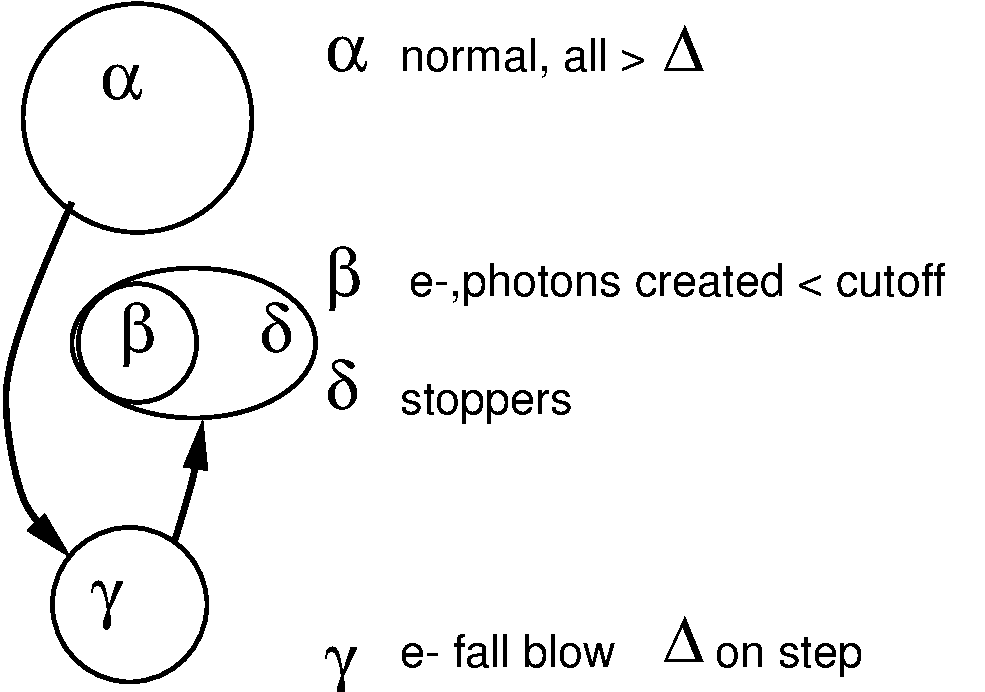
\includegraphics[height=5cm]{figures/sprrz_logic}
\end{center}
\caption[Energy deposition classes in SPRRZnrc]{Modes of energy deposition considered in SPRRZnrc. $\alpha$ events
are those in which energy is deposited by electrons in a step with the
energy entirely above $\Delta$. $\gamma$ events are those in which the
electron starts a step with its energy greater than $\Delta$ and ends with
an energy below $\Delta$. The $\delta$ events are all those events in which
an electron or photon are being terminated because they are below the
cutoffs AE or AP.  This includes a subset of $\beta$ events formed by
electrons and photons which are created with their energy initially below
AE or AP.}
\label{fig_spr_logic}
\end{figure}

The dose delivered by the $\alpha$ events in figure~\ref{fig_spr_logic}
is simple to analyze. In the numerator we just sum the actual energy
deposition. In the denominator we sum the energy deposition times
the ratio of restricted stopping powers at the mid-point energy of the
step, i.e.
\eqn{EDEP \frac{\rspE{Emid}{g}}{\rspE{Emid}{m}}}
This gives how much energy would be deposited in medium $g$ instead of
medium $m$.

The $\beta$ events are not scored at all, except in an evaluation of the
total dose. These events correspond to electrons or photons being created
in the cavity region below the respective transport cut-offs. It is
arguable how to deal with these events, but in traditional calculations
starting from electron spectra they were either ignored or lumped in with
the stoppers.  This issue has been discussed in Borg et al, and there is no
clear solution at this time\cite{Bo99a}.  However, the fraction of the dose contributed
in the cavity region from these events is output by SPRRZnrc and found to
be very small for electron beams or for photon beams at \Co~ energies and
higher. This fact makes the problem academic in most situations.  The
problem becomes serious for low-energy photon beams, but here the
application of Spencer-Attix cavity theory is also suspect\cite{Bo99a}.

The $\delta$ or stopper events which are not $\beta$ events,
are scored as part of the track-end term in
eqn(\ref{eq_sa_spr}).  This is done by scoring the natural energy deposition
in the numerator and the same energy deposition multiplied by the ratio of
the unrestricted stopping powers at $\Delta$ (which are equal to the
restricted stopping powers), i.e.:
\eqn{EDEP \frac{\rspt{g}}{\rspt{m}}.}
Note that this does not merely correspond to the energy deposition in the
second medium, because for a stopper, the energy deposition would be the
same in both media (it just deposits all of its energy which is the same in
both cases). The track-end term in eqn(\ref{eq_sa_spr}) is derived to take
into account that the number of stoppers in each medium will differ because
the fluence of particles stopping in each medium will differ and this
number of stoppers is proportional to the stopping power.

The $\gamma$ events, those particles which cross $\Delta$ during their step
are scored by treating the step as having two components.  The component
with energy above $\Delta$ is treated as if it were an $\alpha$ event and
the component of the energy deposited below $\Delta$ is treated as a
$\delta$ event.

\begin{table}[htb]
\begin{center}
\caption{Energy deposition classes and their components}
\begin{tabular}{|cc|}
\hline
IT value & included events \\
\hline
1  & $\alpha + \gamma + (\delta -\beta)$ \\
3  & $\alpha + \gamma$\\
total & $\alpha + \gamma + \delta$ \\
\hline
\end{tabular}
\end{center}
\end{table}
The SPRRZnrc program scores 3 different doses: the total dose;
dose including everything except the
$\beta$ component (stoppers created below $\Delta$)[IT=1]; dose from
$\alpha$ plus $\gamma$ only [IT=3].
The IT=2 and IT=4 components
correspond to the IT=1 and IT=3 components but scored in the $g$ material
as outlined above. The code then outputs: the total dose; the
fraction of the total dose due to included stoppers (IT=1~$-$~IT=3)/total;
and the fraction of the total dose due to excluded stoppers
(total$-$~IT=1)/total.

The IT=2 dose component is the same as the IT=1 dose component except as
modified to represent the dose in the detector medium as described above.
The IT=4 component similarly corresponds to the IT=3 component, i.e. the
dose less the actual stoppers but including the crossers.

The stopping-power ratios are calculated as the IT=1 dose component divided
by the IT=2 dose component (strictly the scored energy depositions divided
by the respective densities are used).  The stopping-power ratio less the
stoppers is calculated by taking IT=3 divided by IT=4.

The code outputs he two different stopping-power ratios to demonstrate that
the inclusion of the stoppers has only a small effect on the overall
stopping-power ratio, which is a good thing since the treatment of the
stoppers is somewhat arbitrary.  However, it should be pointed out that the
$\gamma$ events are not classified as stoppers but in fact they do contain
some element of the stoppers dose since steps are not stopped at $\Delta$,
but rather at some energy slightly less than $\Delta$.



%\clearpage











\subsection{Input/output control}
\index{SPRRZnrc!I/O control}

I/O control input is delimited between \verb+:start I/O control:+\\
and \verb+:stop I/O control:+.  Most I/O control input
for SPRRZnrc is common to all user codes and is described in
section~\ref{common_I_O_control}\lpage{common_I_O_control}.  However,
the {\tt SPR OUTPUT} control is unique to SPRRZnrc and you input it
as follows:
\begin{verbatim}
  SPR OUTPUT
        = regions         (0)  Specify stopping power ratio output by
                               regions (no .plotdat file will be generated)
        = slabs/cylinders (1)  Specify stopping power ratio output by slabs
                               & cylinders (.plotdat file is generated)
***************************************************************************

  IF SPR OUTPUT= regions

  SPR START REGION   (M)  region numbers in which to start scoring stopping
                           power ratios

  SPR STOP REGION    (M)  region numbers in which to stop scoring stopping
                           power ratios

***************************************************************************

  IF SPR OUTPUT= slabs/cylinders

  SPR IN CYLINDER IX  (M)  Cylinder numbers for which to output
                           stopping power ratios (= 0 for no output)

  SPR IN SLAB IZ      (M)  planar slab numbers for which to output
                           stopping power ratios (= 0 for no output)

**************************************************************************
\end{verbatim}
\index{.plotdat!SPRRZnrc}

\subsubsection{{\tt SPR OUTPUT} options}
\index{SPRRZnrc!SPR OUTPUT}

\index{range rejection!SPRRZnrc}
{\tt SPR OUTPUT} is used to determine how stopping power ratios are
output.  If electron range rejection is off, then stopping power ratios
in all regions are output to the {\tt .egslst} file.  If electron
range rejection is on, then stopping power ratios are zeroed in the
{\tt .egslst} file except in regions specified using
{\tt SPR START REGION} and {\tt SPR STOP REGION} (if
{\tt SPR OUTPUT= regions}) or in slabs/cylinders specified using
{\tt SPR IN CYLINDER IX} and {\tt SPR IN SLAB IZ} (if
{\tt SPR OUTPUT= slabs/cylinders}).  In addition, electron range rejection
is automatically turned off in the regions/slabs/cylinders you have selected
for output so that the stopping power ratios will be meaningful.  If you
are using the {\tt SPR OUTPUT= slabs/cylinders} option, then you will also
get a {\tt inputfile\_dd.plotdat} file which contains the stopping power ratios (and
doses) in the selected slabs and a {\tt inputfile\_rad.plotdat} file
containing stopping power ratios (and doses) in the selected cylinders.
This files are in a format that can be plotted
with {\tt xmgrace} or other plotting program.
\index{.plotdat!SPRRZnrc}

\subsection{Monte Carlo control}
\index{SPRRZnrc!Monte Carlo control}

Monte Carlo control input is delimited between
\verb+:start Monte Carlo inputs:+\\
and \verb+:stop Monte Carlo inputs:+. In addition to the Monte Carlo inputs
common to all user codes (see section~\ref{MC_inputs}\lpage{MC_inputs}),
SPRRZnrc has the following Monte Carlo input:
\begin{verbatim}
  PHOTON REGENERATION         (C)  yes => primary photons are regenerated
                                          after they interact and scattered
                                          photons are thrown away.
                                   no (default) => full calculation

\end{verbatim}
\index{photon regeneration!SPRRZnrc}

\subsubsection{{\tt PHOTON REGENERATION} option}
\index{SPRRZnrc!photon regeneration}
\label{photregsect}

The photon regeneration option is used to calculate the stopping power ratios
for electrons resulting from an unattenuated and unscattered photon beam.
If {\tt PHOTON REGENERATION= yes}, then, prior to a pair production,
compton, photoelectric or Rayleigh event, the properties of the photon about
to interact are saved.  After the interaction, any scattered photons or
photons resulting from relaxation process are discarded and (once all
secondary electrons have been transported) transport reverts to the duplicate
photon that was saved just before the interaction.  In addition, photons
resulting from bremsstrahlung events and positron annihilation events are
eliminated on the spot.
%, and positrons resulting from pair events are
%converted to electrons.
%\note{Why are positrons made into electrons in photon regeneration?}
%\note{Same occurs in general? WHY?????}

This option is to be used when calculating stopping-power ratios for use
in air kerma cavity ion chamber standards since the basic theory makes this
assumption. This makes the calculated stopping-power ratio independent of
the details of the geometry as long as there is full buildup.  This is
discussed in detail by Borg et al\cite{Bo99a}.  This option should not be
used when calculating stopping-power ratios in a phantom since in that case
you want the effects of scatter and attenuation to be taken into effect.


%\renewcommand{\rightmark}{{CAVRZnrc}}
%%%%%%%%%%%%%%%%%%%%%%%%%%%%%%%%%%%%%%%%%%%%%%%%%%%%%%%%%%%%%%%%%%%%%%%%%%%
\section{CAVRZnrc}
%%%%%%%%%%%%%%%%%%%%%%%%%%%%%%%%%%%%%%%%%%%%%%%%%%%%%%%%%%%%%%%%%%%%%%%%%%%
\renewcommand{\leftmark}{{CAVRZnrc}}
\index{CAVRZnrc}

\subsection{Introduction}

CAVRZnrc calculates various factors of interest when using cavity ion
chambers such as $A_{att}$ and $A_{scat}$ and $A_{wall}$.
It has been described in detail in various
publications\cite{Bi85,Ro85a,RB90a,Bi90a} and shown to produce results in
good agreement with standard theory\cite{Bo99a}.

\subsection{Cavity inputs}
\index{CAVRZnrc!cavity inputs}

CAVRZnrc requires an extra set of
inputs defining the cavity region.  These inputs must appear between the
delimiters {\tt :start cavity inputs:} and {\tt :stop cavity inputs:}.

If the user has input the radial geometry using
{\tt METHOD OF INPUT= individual} or {\tt METHOD OF INPUT= groups}
(see section~\ref{geomsect}\lpage{geomsect}), then the following inputs must
appear between the cavity input delimiters:
\begin{verbatim}
   NUMBER OF CAVITY REGIONS (I)   number of geometrical zoneS
                                  comprising the cavity.

   REGION NUMBERS OF THE CAVITY  (M)
                                  the array of these zones
                                  (the cavity region numbers)
\end{verbatim}
Thus, the user defines the cavity in terms of region numbers within the
geometry.

Alternatively, CAVRZnrc offers another method for entering the geometry
in which the geometry is
automatically defined based on cavity information specified by the user.
In this case, only {\tt METHOD OF INPUT= cavity information} needs to be
entered between the {\tt :start geometrical inputs:} and
{\tt :stop geometrical inputs:} delimiters.  Then, between the
cavity input delimiters, the following inputs must be supplied:

\begin{verbatim}

   WALL THICKNESS      (R)   thickness of the chamber walls (cms)
                             (defaults to 0.273)

   CAVITY RADIUS       (R)   outer radius of the cavity (cms)

   CAVITY LENGTH       (R)   length of the cavity (cms) (defaults to 0.2)

   ELECTRODE RADIUS    (R)   radius of the electrode (defaults to 0.)

   WALL MATERIAL       (C)   wall material

   only if   ELECTRODE RADIUS > 0.0
   ELECTRODE MATERIAL  (C)   electrode material
\end{verbatim}
CAVRZnrc creates a simple 3-cylinder
({\tt RCYL(1)=ELECTRODE RADIUS, RCYL(2)=\\CAVITY RADIUS, RCYL(3)=
CAVITY RADIUS + WALL THICKNESS}), 3-slab ({\tt ZPLANE(1)=0,\\
ZPLANE(2)=WALL THICKNESS, ZPLANE(3)=WALL THICKNESS + CAVITY LENGTH,\\
ZPLANE(4)=2*WALL THICKNESS + CAVITY LENGTH}) geometry based on these
inputs.  The material in the cavity is assumed to be AIR.  This option was
useful for early calculations but is not adequate for chambers in which we
want to include much detail.

\subsection{Input/output control}
\index{CAVRZnrc!I/O control}
\label{cavrziosect}

As with the other user codes, I/O control inputs must appear within
the delimiters {\tt :start I/O control:} and {\tt :stop I/O control:}.
In addition to I/O controls that are common to all user codes (see
section~\ref{common_I_O_control}\lpage{common_I_O_control}), CAVRZnrc
has the following inputs:
\begin{verbatim}
  STORE INITIAL RANDOM NUMBERS
        = no          (0)  do not store initial random numbers
        = last        (1)  store initial random number for last history
        = all deposited (2)store the initial random number for all
                           that deposit energy in the cavity
        = all         (3)  store all the initial random numbers

  OUTPUT OPTIONS
        = short              (0)  short output -just the cavity summary
                                  and the dose grid.
        = cavity details     (1)  above plus details for each cavity zone
\end{verbatim}
\index{CAVRZnrc!store initial random numbers}
The {\tt STORE INITIAL RANDOM NUMBERS} input has been included here because
CAVRZnrc has one option, {\tt STORE INITIAL RANDOM NUMBERS= all deposited},
that is not included in the other user codes (see
section~\ref{rnssect}\lpage{rnssect}).
With this option, the initial random numbers from only those histories that
end up depositing energy in the cavity region are stored in the
{\tt .egsrns} file.  Then, if the run is restarted with
{\tt IRESTART= start-RNS} (see section~\ref{restartsect}\lpage{restartsect}),
all histories will end up depositing energy in the cavity region.

\index{CAVRZnrc!output options}
If the user chooses {\tt OUTPUT OPTIONS= short}, then dose and correction
factors will only be output for the cavity as a whole.  If
{\tt OUTPUT OPTIONS= cavity details}, then dose and correction factors
will be output for the cavity as a whole and for each region that makes up
the cavity.

\subsection{Monte Carlo control}
\index{CAVRZnrc!Monte Carlo control}

Monte Carlo control input is delimited between
\verb+:start Monte Carlo inputs:+\\
and \verb+:stop Monte Carlo inputs:+.  In addition to Monte Carlo inputs that
are common to all user codes (see
section~\ref{MC_inputs}\lpage{MC_inputs}), CAVRZnrc had the following
Monte Carlo inputs:
\begin{verbatim}
  IFULL
         = dose and stoppers     (0) just calculate total dose
         = Aatt and Ascat        (1) Above plus Aatt, Ascat
         = Ap                    (2) Above plus Ap as well (option
                                     currently disabled)
         = Afl and <s>g/w        (3) Above plus Afl and <s>g,w as well
                                     (option currently disabled)

  STATISTICAL ACCURACY SOUGHT    (R) % statistical accuracy of the total
                                     dose in the peak region that is
                                     sought The program executes until this
                                     accuracy is obtained or the CPU time
                                     runs out.
  PHOTON REGENERATION
         = yes (1) the calculation is performed with regeneration
                           of the parent photon after they have
                           interacted. A typical setting when FANO
                           conditions are examined.
         = no (0)  a normal calculation.
         = no electrons from wall (ifano = 2) secondary electrons from
                           interactions in the cavity wall are immediately
                           eliminated.  Photons are not regenerated.
                           [IFANO]
\end{verbatim}
\index{photon regeneration!CAVRZnrc}

\subsubsection{{\tt IFULL= dose and stoppers} option}
\index{CAVRZnrc!IFULL}
\index{CAVRZnrc!output of dose}
\label{cavrzifullsect1}

If {\tt IFULL= dose and stoppers}, then CAVRZnrc will output the total
dose in the cavity and, if {\tt OUTPUT OPTIONS= cavity details},
in each region making up the cavity to the {\tt .egslst} file.

\subsubsection{{\tt IFULL= Aatt and Ascat} option}
\index{CAVRZnrc!output of $A_{att}$ and $A_{scat}$}
\label{cavrzifullsect2}

The methods used to calculate the various correction factors have been
described in the literature\cite{Bi85,Ro85a,Bi86,RB90a}.
%\note{This section on Awall needs to be completed .}

If {\tt IFULL= Aatt and Ascat}, then CAVRZnrc will output the total dose,
$A_{att}$, $A_{scat}$ and $A_{wall}$ in the cavity and, if {\tt OUTPUT
OPTIONS= cavity details}, in each region of the cavity to the {\tt
.egslst} file. The listing files also include $K_{wall} = 1./A_{wall}$
(etc).

The scatter correction factor, A$_{scat}$, is defined as the ratio of the
total energy deposited in the cavity to the energy deposited by electrons
generated by primary photon interactions~\cite{Bi86}.  In CAVRZnrc,
photons are flagged as secondary if they have been scattered in compton,
or Rayleigh events, generated by bremsstrahlung or positron annihilation
events, generated by atomic relaxations after compton or photoelectric
events, or if their energy is deposited locally because they have
energy $<$ N-shell energy in a photoelectric event.  Once CAVRZnrc has
totalled the energy deposited in the cavity by electrons generated by
primary photons (ECAV$_{prim}$), and the energy deposited in the cavity
by electrons generated by photons flagged as secondary (ECAV$_{sec}$),
A$_{scat}$ is calculated using the equation:

\begin{equation}
A_{scat}=1+\frac{ECAV_{sec}}{ECAV_{prim}}
\end{equation}

\subsubsection{{\tt STATISTICAL ACCURACY SOUGHT}}
\index{CAVRZnrc!statistical accuracy sought}

If you input a value for {\tt STATISTICAL ACCURACY SOUGHT}
other than zero, then CAVRZnrc will stop when the percent uncertainty on the
total dose in the cavity volume (all cavity regions combined) is equal
to {\tt STATISTICAL ACCURACY SOUGHT} provided that
{\tt NUMBER OF HISTORIES} (see section~\ref{histsect}\lpage{histsect})
or {\tt MAX CPU HOURS ALLOWED} (see section~\ref{cpusect} \lpage{cpusect}) have
not been reached first.

\subsubsection{{\tt PHOTON REGENERATION} options}
\index{photon regeneration!CAVRZnrc}

CAVRZnrc offers two photon regeneration options.  If the user selects
{\tt PHOTON REGENERATION= yes}, then photon regeneration is similar to
that in SPRRZnrc (see section~\ref{photregsect}\lpage{photregsect}).
Unlike SPRRZnrc, where it is required for proper
stopping power ratio calculations as used in primary
air-kerma standards, the purpose of this option in CAVRZnrc is
mainly for theoretical benchmark calculations ({\em e.g} testing
for artefacts under Fano conditions). An additional use
could be for an independent verification of $A_{wall}$: one
runs simulations with {\tt PHOTON REGENERATION= ON} and {\tt PHOTON
REGENERATION= OFF}, the
ratio of the two doses is per definition $A_{wall}$. This is
however not very efficient and a better way to accomplish
this task is to use the cross section enhancement or
photon splitting options described below.

The second regeneration option in CAVRZnrc is {\tt PHOTON REGENERATION= no
electrons from wall}.  With this option, charged particles resulting from
pair production, compton and photoelectric events are eliminated provided
that the interaction did not take place inside the cavity.
This is a hack that has been used to study
the dose fraction from photon interactions in the cavity.

\subsection{CAVRZnrc variance reduction techniques}

\subsubsection{Photon cross section enhancement}
\label{cavrz_cse}
\index{cross section enhancement!CAVRZnrc}
\index{CAVRZnrc!cross section enhancement}

The cross section enhancement technique in CAVRZnrc is
similar to the one implemented in DOSRZnrc
(see section \ref{dosrz_cse} page~\pageref{dosrz_cse}) but
in CAVRZnrc it is applied globally in the entire geometry and the value of
$C_e$ is input directly (as opposed to C as input in the DOSRZnrc case).
Cross section enhancement in CAVRZnrc can be turned on by
including the following line in the input file:
\begin{verbatim}

  CS ENHANCEMENT FACTOR=  some real number [cs_enhance]

\end{verbatim}
If the input is missing or less than unity, there will be
no effect.  But if the enhancement factor is set to greater than unity, the
effect is dramatic: all other user input concerning photon forcing,
splitting, exponential transform, etc., is ignored. In addition,
the calculation result \underline{always} corresponds
to the {\tt IFULL= Aatt and Ascat} option, no matter what the
user requested (but only $A_{wall}$ is calculated,
not the individual $A_{scat}$ and $A_{att}$, see
section \ref{cavrzifullsect2}). In addition, all scoring
is done using proper history-by-history statistics using
the common block {\tt score1}.  The drawback is that dose
and $A_{wall}$ are calculated for the whole cavity and
not on a region-by-region basis as under normal
CAVRZnrc operation.

The following text gives a brief description of the differences
to the DOSRZnrc implementation: The motivation behind the
implementation of cross section enhancement in CAVRZnrc was the desire to
have an independent calculation technique for $A_{wall}$ that is
not too inefficient compared to the unweighting technique. Indeed,
$A_{wall}$ can be calculated by running two separate CAVRZnrc
simulations, one with normal transport  and one with attenuation
and scatter removed via the {\tt photon regeneration= on} option. The ratio of the
cavity dose from the former to the dose from the latter calculation is by
definition $A_{wall}$. Because both calculations
are uncorrelated, their uncertainties add in quadrature and so, the uncertainty
on $A_{wall}$ is larger than the individual dose uncertainties.
The purpose of the cross section enhancement implementation in
CAVRZnrc is to make the two necessary dose calculations at once
and thus reduce the uncertainty of $A_{wall}$ because of the strong
correlation between the ``normal'' dose and the dose with
attenuation and scatter removed. To accomplish this task,
scattered photons are killed as in DOSRZnrc with probability
$1/C_e$. If they survive, they are marked as scattered by setting
their {\tt latch} variable to 3. Unlike in DOSRZnrc, the unscattered
portion of primary photons is always kept on the stack and transported.
However, these non-scattered fractions of primary photons are marked
as attenuated primary photons ({\tt latch=2}) with probability
$1-1/C_e$ and therefore their descendents only contribute to the
dose with attenuation and scatter removed. In addition, scatter,
bremsstrahlung and annihilation from {\tt latch=2} particles are
immediately removed from the stack. It is then clear that
{\tt latch=0,2} electrons contribute to the dose with
attenuation and scatter removed, {\tt latch=0,3} electrons to
the normal dose.

\subsubsection{Photon splitting}
\index{photon splitting!CAVRZnrc}
\index{CAVRZnrc!photon splitting}
\label{cavrzsplitsect}

An additional variance reduction scheme offered in CAVRZnrc
is the photon splitting technique.
Input that turns on photon splitting must appear
between the {\tt :start variance reduction:}
and {\tt :stop variance reduction:} delimiters and is:

\begin{verbatim}

 PHOTON SPLITTING=    (I)    Number of times to split a photon
                             If missing or < 2  => normal transport
                             If >= 2 (allowed only for ifull= dose and
                             stoppers or = Aatt and Ascat), the macro
                             $SELECT-PHOTON-MFP essentially replaces the
                             entire PHOTON routine.
                             [n_split]

\end{verbatim}

This technique is borrowed from Ref. \cite{KF99} where it was shown
to increase the efficiency of external photon beam calculations for
radiotherapy by up to a factor of 5. The increase in CAVRZnrc is
not so dramatic, nevertheless an increase in the efficiency
of cavity dose calculations of up to a factor of 3 compared to using photon
forcing has been observed.

This option is only available with {\tt IFULL= dose and stoppers or =Aatt and Ascat}.
It is also possible to use the {\tt ifano} option (only
if {\tt IFULL=0}). Note that with photon splitting
on, all scoring
is done using proper history-by-history statistics using
the common block {\tt score1}.  The drawback is that dose
(and $A_{wall}$ if requested) are calculated for the whole scoring cavity and
not on a region-by-region basis as under normal CAVRZnrc operation.

The algorithm works as follows:
each photon that is to be transported is split into
{\tt n\_split} photons with weights $w_0/${\tt n\_split}
($w_0$ is the original photon weight). The number of
mean-free-paths $\lambda_i$ to the next interaction of the $i$'th
such photon is sampled from
\begin{equation}
\lambda_i = -\ln \left[1 - {\xi + i - 1 \over {\tt n\_split} } \right]
\end{equation}
where $i$ runs from 1 to {\tt n\_split} and where $\xi$ is a random
number. This forces a uniform distribution of interaction sites.
In addition we have $\lambda_{i+1} > \lambda_i$ and therefore
only transport from $\lambda_i$ to $\lambda_{i+1}$ is needed to
get to the interaction site of the $i+1$'st photon from the
interaction site of the $i$'th photon. When one of the split-photons
interacts, all resulting scattered photons are killed with probability
1/{\tt n\_split} and marked as scattered if they survive
({\tt latch=3}). If {\tt IFULL= Aatt and Ascat} or {\tt photon
regeneration= on}, the original photon is
re-created at each interaction site with probability
1/{\tt n\_split} and marked as a regenerated photon ({\tt latch=2}).
As for the cross section enhancement technique, {\tt latch=0,3} particles
contribute to the normal dose, {\tt latch=0,2} particles to the dose
with attenuation and scatter removed. The ratio of the two is
$A_{wall}$ and so, photon splitting is a third independent
technique for calculating this quantity.

A rule of thumb for good efficiency is to use
\eqn{n\_split \ge \frac{N_o}{1. - e^{-\lambda}} }
where $\lambda$ is approximately the number of photon mean free paths in the
geometry of interest and $N_o \ge 5$. For $^{60}$Co, $\lambda$ is about
0.06 for 1 g/cm$^2$ of graphite and so $n\_split$ should be $\ge 80$.

%%%%%%%%%%%%%%%%%%%%%%%%%%%%%%%%%%%%%%%%%%%%%%%%%%%%%%%%%%%%%%%%%%%%%%%%%%%%%
\section{Spherical user codes}
%%%%%%%%%%%%%%%%%%%%%%%%%%%%%%%%%%%%%%%%%%%%%%%%%%%%%%%%%%%%%%%%%%%%%%%%%%%%%

\subsection{Introduction}

Since 2003, the EGSnrc distribution includes a pair of spherical
geometry user codes.
CAVSPHnrc is the spherical analogue of CAVRZnrc, designed for ion chamber
calculations, and has been used extensively for this purpose (see, \eg,
references\cite{Bi90b,RT99}). The other code, EDKnrc, was derived from
SCASPH, an EGS4 user code for the calculation of mono-energetic energy
deposition kernels\cite{Ma88}. EDKnrc has been extended to allow the use
of both monoenergetic and polyenergetic sources.

Both user codes share most of the common features of the RZ user codes
excluding geometry and source types. We will describe these two in the
following subsections and the user is refered to section \ref{Common}
for information on the common input blocks of these codes.

\subsection{Geometry and Material Inputs}

\subsubsection{Geometrical input: spheres and cones}

The geometrical regions subtended by concentric spheres and cones
originating at the common center of the spheres are shown in figure
\ref{fig_spherical}. NR represents the number of spheres and NC the
number of cones. In what follows we explain the input specification of
the geometry.


\begin{figure}[hbt]
\htmlimage{scale=1.2}{}
\begin{center}
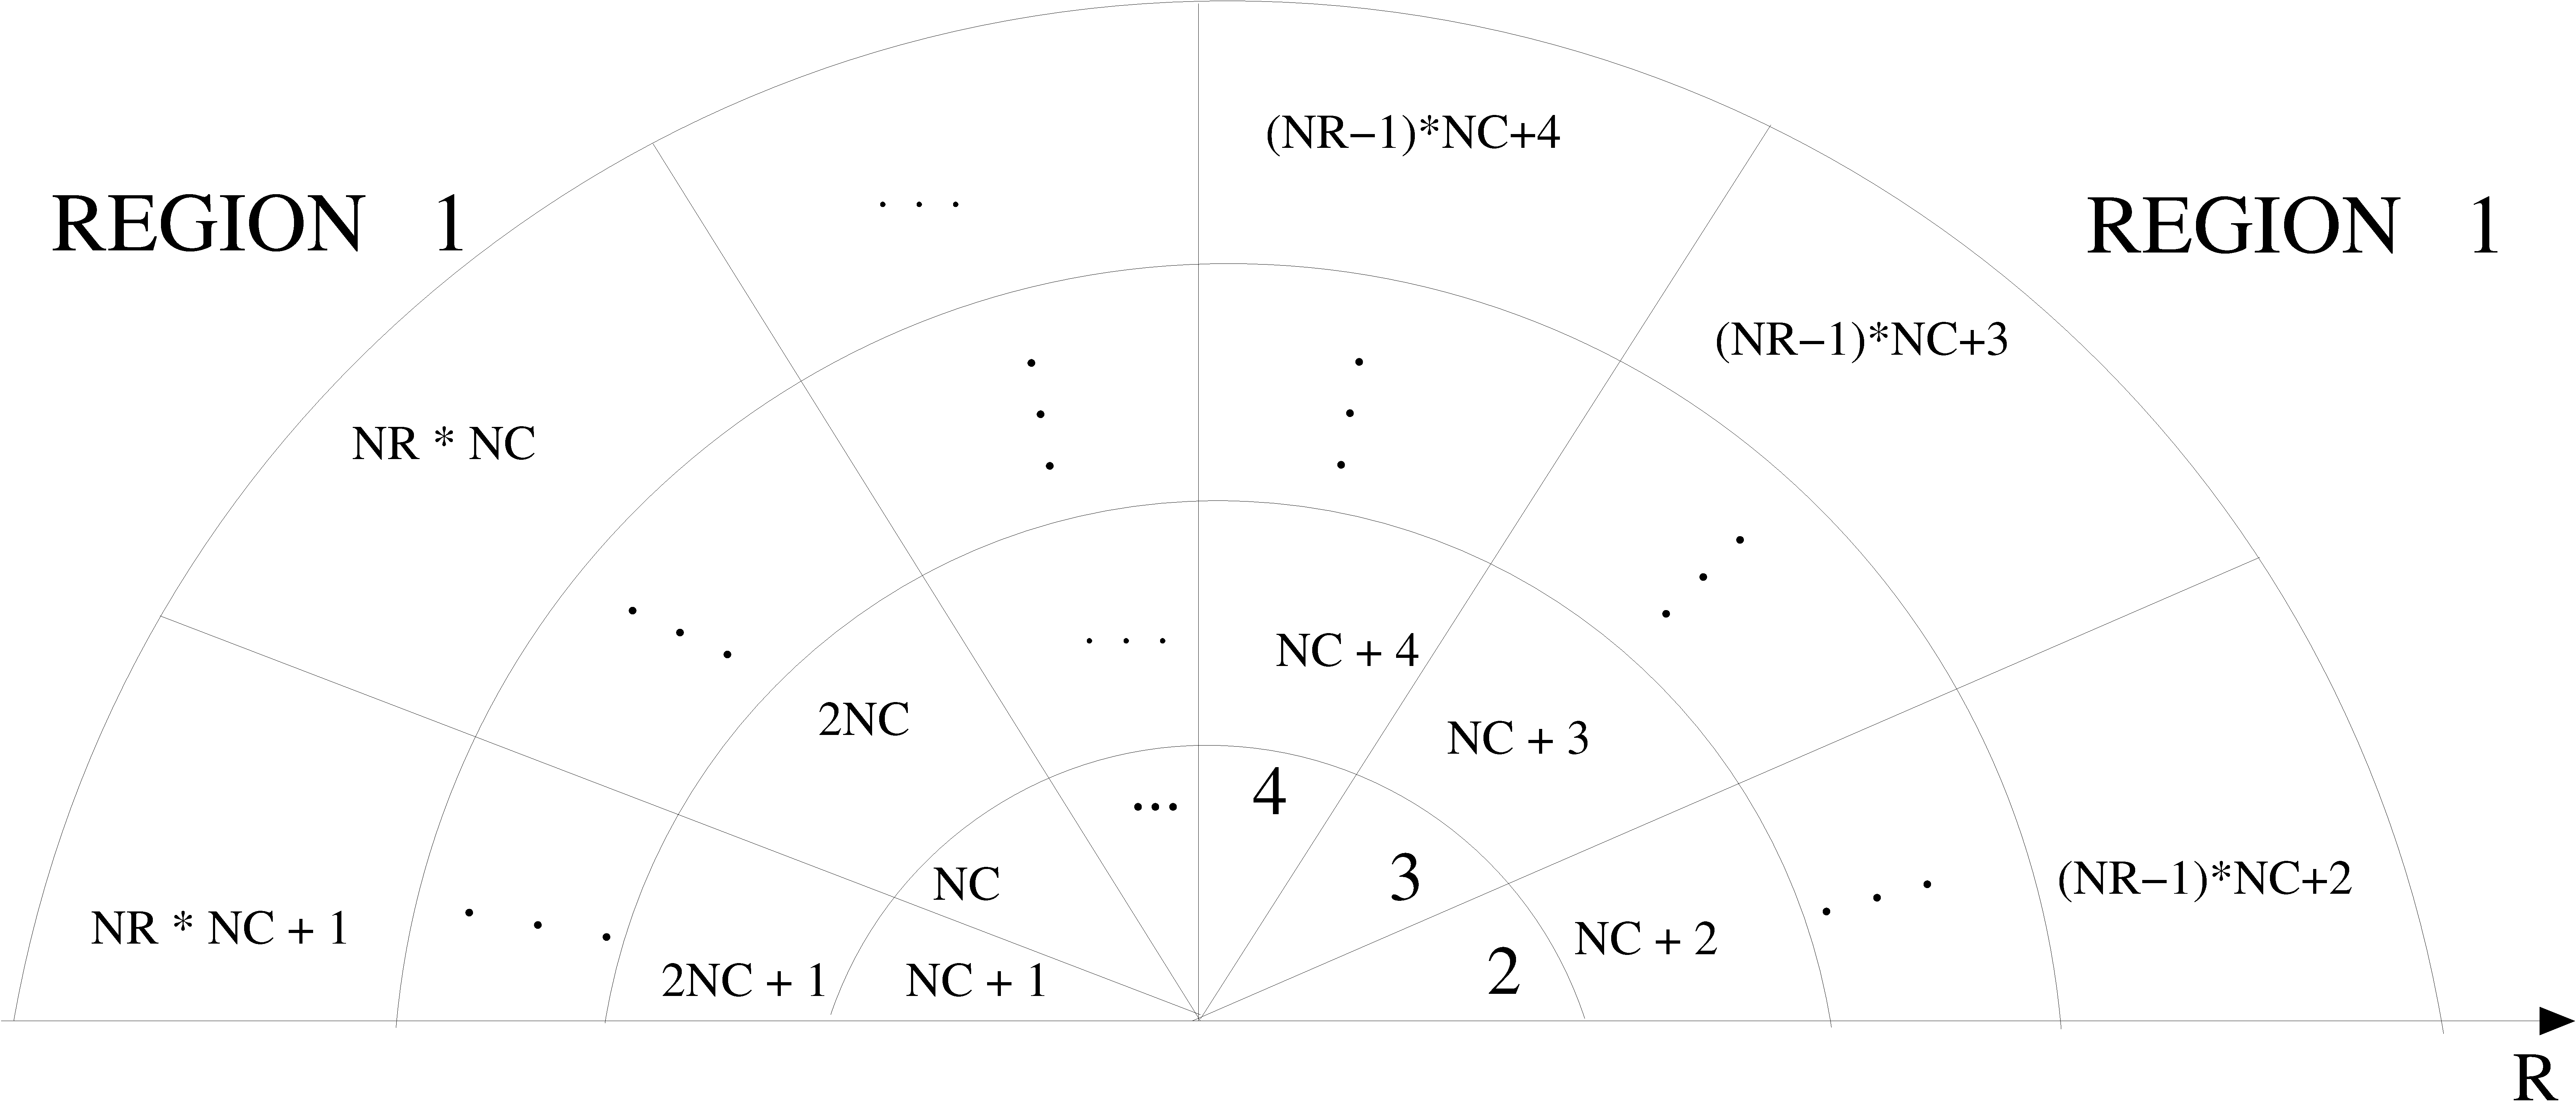
\includegraphics[height=5cm]{figures/spherical}
\end{center}
\caption[Spherical geometry]{Region numbering scheme for the spherical
user codes.  Region number 1 is always outside the geometry. The first
region (2) is defined by the innermost sphere and the cone with the
smallest opening angle. {\tt NR} is the number of radial zones = \# radii
and {\tt NC} = number of cones (0 for purely spherical geometry). }
\label{fig_spherical}
\end{figure}

As in the RZ codes, the geometry inputs are delimited by the strings
{\tt :start geometrical inputs:} and {\tt:stop geometrical inputs:}. The
meaning of the inputs depends on the entries for {\tt NUMBER OF CONES}  and
{\tt NUMBER OF SPHERES}. If a single value is input, then the user is
expected to input the individual corresponding radii or angles. If multiple
values are given for {\tt NUMBER OF CONES}  and/or {\tt NUMBER OF SPHERES},
the user is expected to put in groups of equal angles and/or radii.
If, for instance, several
entries are made for the number of angles, \ie, {\tt NANG1, NANG2, ...}, it
is assumed that the first {\tt NANG1} cones will have the same opening angle
and so on. For spheres, if the user omits the number of radii, it is
assumed that individual entries will be made (after all,
these are user-codes for spherical problems).

\begin{verbatim}
 NUMBER OF CONES= [NANG(1)[,NANG(2),...,NANG(K)]]
                  # If omitted or ZERO, pure spherical geometry assumed
 NUMBER OF SPHERES= [NRAD(1)[,NRAD(2),...NRAD(J)]]
                  # no needed for individual input
\end{verbatim}

Once the user has defined the number of spheres and cones in the problem, the
actual values for the radii and angles must be entered, using the keywords
outlined below:

\begin{verbatim}
RADII= RAD(1), RAD(2), ...RAD(j)
                  #radii of spheres defining the geometry
                  #For group input there must be as many entries
                  #as for the NUMBER OF SPHERES, i.e. :
                  #         J = j
                  #For individual input, NRAD(1) must be equal
                  #to the number of entries, i.e.:
                  #        NRAD(1) = j
                  #unless NUMBER OF SPHERES is omitted, in which case
                  #indiviual input is automatically assumed.
ANGLES= ANG(1), ANG(2),...,ANG(3)
                  #The same rules apply for angles as for radii apply.
\end{verbatim}

One can also enter a group of regions to be considered as the cavity
of a spherical ion chamber and the total dose in these regions will
be computed. For CAVSPHnrc, quantities such as
$K_{att}$ and $K_{scat}$ and $K_{wall}$ are also calculated for the
whole cavity. The specification for the cavity inputs is:
\begin{verbatim}
CAVITY ZONES= [REG1[, REG2...,REGn]] #geometrical zones defined as the
                                     #cavity (real numbers)
\end{verbatim}

\subsubsection{Material input.}

These codes have a simple structure for entering the material input. First
the user must provide a list of media in the problem where the first
medium is taken as default, \ie, every region is considered to have this
medium. Then, medium numbers for all regions where the medium is not
medium 1 must be specified.


\begin{verbatim}
 MEDIA= MEDIUM1, MEDIUM2,..., MEDIUMn

 MEDNUM=        MEDIUM2, MEDIUM2, MEDIUM3,..., MEDIUMn
 START REGION=  START1,  START2,  START3,...,  STARTn
 STOP REGION=   STOP1 ,  STOP2,   STOP3, ...,  STOPn

\end{verbatim}

\subsection{CAVSPHnrc}
The NRC user code CAVSPHnrc (spherical geometry) like CAVRZnrc
(cylindrical geometry) calculates various factors of interest when using
ion chambers such as $K_{att}$, $K_{scat}$, $K_{wall}$ and the dose to the
cavity region per unit incident fluence.

The input file for this user code is very similar to the one for
CAVRZnrc. Only two input blocks are different, the geometry input block
and the input block for the sources. The geometry input was described
previously and the input for the sources differ from CAVRZnrc, in that
only four source types are available: a parallel beam from any angle
(source 0), a point source from any angle (source 1), a parallel beam
from any angle with radial distribution (source 10), a point source from
any angle with radial distribution (source 11).
and a point source from any angle. The source input block is defined by
the delimeters {\tt :start source inputs:} and {\tt :stop source inputs:}
and the same inputs are needed as in CAVRZnrc (see
section~\ref{source_inputs} on page~\pageref{source_inputs}).  In
particular, one must define:

\begin{verbatim}
  INCIDENT PARTICLE= electron   (-1)  electrons
                     photon     (0)   photons
                     positron   (1)   positrons

  SOURCE NUMBER                 (I)   number of the source
                                      [ISOURC]
  SOURCE OPTIONS                (M)   four or five real numbers as specified
                                      below

------------------------------------------------------------------------------

 SOURCE 0/10:  FOR PARALLEL BEAM FROM ANY ANGLE (10-->WITH RAD. DISTN)
              RBEAM,UINC,VINC,WINC
               RBEAM   RADIUS OF THE BEAM AT THE FRONT OF THE TARGET IN CM
                               DEFAULTS TO MAX RADIUS
               UINC    INCIDENT X-AXIS DIRECTION COSINE
               VINC    INCIDENT Y-AXIS DIRECTION COSINE
               WINC    INCIDENT Z-AXIS DIRECTION COSINE
                       NOTE: (UINC,VINC,WINC) GET AUTOMATICALLY NORMALIZED
                             DEFAULTS TO (0.0,0.0,1.0)
------------------------------------------------------------------------------

 SOURCE 1/11:  FOR POINT SOURCE INCIDENT FROM ANY ANGLE (11-->WITH RAD. DISTN)
             DISTR,RBEAM,UINC,VINC,WINC
               DISTR   DISTANCE OF THE SOURCE FROM THE MIDDLE OF THE TARGET
                       IN CM (DEFAULTS TO 100.)
               RBEAM   RADIUS OF THE BEAM AT THE FRONT OF THE TARGET IN CM
                               DEFAULTS TO MAX RADIUS
               UINC    INCIDENT X-AXIS DIRECTION COSINE
               VINC    INCIDENT Y-AXIS DIRECTION COSINE
               WINC    INCIDENT Z-AXIS DIRECTION COSINE
                       NOTE: (UINC,VINC,WINC) GET AUTOMATICALLY NORMALIZED
                             DEFAULTS TO (0.0,0.0,1.0)
------------------------------------------------------------------------------

 SOURCE 10 OR 11:
       SPECIFY MODE:
               MODE = local (0)     IF RADIAL DISTRIBUTION IS TO BE INPUT
                                    LOCALLY WHETHER THROUGH THE KEYBOARD
                                    (INTERACTIVE USE) OR THROUGH THE
                                    .INP FILE (DEFAULT)
                    = external (1)  IF THE DISTRIBUTION IS TO BE INPUT
                                    VIA AN EXTERNAL FILE
       IF MODE=local SPECIFY:

           RDISTF(I)= TOP OF RADIAL BIN I FOR I=1,NBIN
           RPDF(I)= PROBABILITY OF INITIAL PARTICLE BEING IN BIN I FOR
                    I=1,NBIN.

                      PROBABILITIES DO NOT NEED TO BE NORMALIZED
                      BUT SHOULD BE IN UNITS CM**-2

       IF MODE=external SPECIFY:

           RDIST FILNAME = FILENAME(WITH EXT) CONTAINING THE ABOVE INFORMATION


       SPECIFY:
           DISTRIBUTION DATA = NONE => NO DISTRIBUTION DATA IN OUTPUT SUMMARY
                             = OUTPUT SUMMARY => INCLUDE DISTRIBUTION
                               DATA IN OUTPUT SUMMARY
\end{verbatim}

\subsection{EDKnrc}

The NRC user code EDKnrc can be used to calculate Energy Deposition Kernels
for photons or electrons (monoenergetic or polyenergtic) forced to interact
at the centre of a spherical
geometry\cite{Ma05}.  The code can output energy deposition kernels (EDK),
dose distributions in the phantom or the dose to regions defined as the
cavity of a spherical ion chamber.  Voxels are defined by the intersection
of a spherical shell with two cones. See figure \ref{fig_spherical}
for more details.

Although the geometry inputs for this user code are similar to CAVSPHnrc,
there are some major differences in other inputs. The input block for I/O
control, defined by the delimeters {\tt :start I/O control:} and
{\tt:stop I/O control:}, is severely abbreviated.  It includes an entry,
{\tt PRINT OUT EDK FILE} that defines whether energy deposition
kernels will be output in the same format as the ones calculated by
Mackie {\it et al.}\cite{Ma88}. The entire input for this block
is shown below:

\begin{verbatim}

:start I/O control:
  IRESTART
       = first    (0) First run for this data set
       = restart  (1) Restart a previous run
       = analyze  (3) Just read in the raw data and do the statistical analysis
       = parallel (5) Combine results from previous parallel runs
  STORE DATA ARRAYS
       = yes             (0) Store data arrays for re-use
       = no              (1) don't store them
  PRINT OUT EDK FILE
       = yes             (0) EDK stored in old format files
       = no              (1) don't produce EDK files in old format
:stop I/O control:
\end{verbatim}


The input block defining Monte Carlo parameters (delimited by
{\tt start}/{\tt stop Monte Carlo inputs:}) is also abbreviated.  Here
one specifies only the number of histories, the initial random number
seeds, and a variable {\tt IFULL}, which specifies the type of calculation,
and an input specifying whether doppler broadening is to be taken into
account during Compton interactions.

\begin{verbatim}

IFULL= cavity calculation        #(0) calculate dose in cavity regions
     = energy deposition kernels #(1) calculate and output EDK's
     = dose calculation          #(2) calculate and output dose
     = dose and edk              #(3) calculate and output EDK's and dose

DOPPLER BROADENING= On
                  = Off

\end{verbatim}

EDKnrc allows for only three possible sources: 1) a photon source algorithm
that forces photons moving along the Z-axis to interact at the origin
(source 0) 2)
an isotropic point source at the origin for any type of
particle (source 1) 3) same as source 0 but with interaction point shifted
to a user-specified position on the Z-axis (source 2).  Source 2
was left for comparison with older EDK calculations, but the user
is strongly discouraged from using it, since it has been shown to produce
numerical artifacts when computing EDK's. For accurate EDK calculations
source 0 should be used.   The inputs specifying the source type, which is
included within the {\tt start}/{\tt stop Source Inputs:} delimiters,
are shown below:

\begin{verbatim}
SOURCE NUMBER= 0 | 1 | 2
#     0 ==>  Photon moving along Z axis forced to interact at origin
#     1 ==>  Point source at origin, isotropically radiating into 4 Pi
#     2 ==>  Same as 0 but interaction point as in old code

# if SOURCE NUMBER= 2
    ZIN      #-> source offset on Z-axis
             #   Option used to emulate old way of calculating EDK
\end{verbatim}

Note that in the case of source 0 or source 2, the {\tt INCIDENT PARTICLE=}
(standard for all user codes when specifying the source) input must be
set to {\tt PHOTON}.

The energy deposited in the geometry can be separated into different
contributions from each photon scattering order (\eg~ primary,
first scatter, second scatter, multiple scatter and radiative). For
electrons, the deposited energy can be split into primary and radiative
contributions. In the standard output file {\tt *.egslst}, only the total
and primary components are written. ONLY if the user selects the option
for creating old format EDK files, all components are stored to a file
following the convention:
\begin{itemize}
\item {\tt edk[EIN].keV}, for monoenergetic sources,
where EIN is the initial energy in keV.
\item {\tt file\_name.keV}, for polyenergetic sources (spectrum),
where {\tt file\_name} is the standard output file name

\end{itemize}

The user also has the choice to
create xmgrace plot files for the {\bf total dose} by using the input block for plot control delimited by
{\tt :start plot control:} and {\tt:stop plot control:}. A description of this input block is
given below:

\begin{verbatim}
   :start plot control:

   PLOTTING
          = Off         (0)   no plots or plot files to be prepared
          = Histogram   (1)   histogram plotting
          = Point       (2)   xy graph


  ONLY IF not PLOTTING= Off

   PLOT RADIAL REGION IX  (M)  radial regions to plot vs angle
                               (= 0 for no plots)

   PLOT CONICAL REGION IC  (M)  angular intervals to plot vs radius
                               (= 0 for no plots)

   :stop plot control:
\end{verbatim}

Plots in radial regions are written to the file {\tt inputfile.angplot}
({\em i.e.} dose versus angle) and plots in conical regions are written
to the file {\tt inputfile.radplot}.

The output capabilities of this user code are very limited but can be
easily extended to print out all components of the energy deposition
kernels.

\typeout{}
\typeout{***Start of Cited References****}
\typeout{}
\renewcommand{\leftmark}{{REFERENCES}}
\renewcommand{\rightmark}{{REFERENCES}}
\section{References}
\vspace*{-1.7cm}
\bibliography{../irs}
%above points to where we find the master reference list
\typeout{}
\typeout{******REMEMBER to create .bbl  and reset twice**********}
\typeout{}
\bibliographystyle{unsrt}


\newpage
\typeout{**********starting index here******************}
\renewcommand{\leftmark}{{Index}}
\renewcommand{\rightmark}{{Index}}
\addcontentsline{toc}{section}{\numberline{}Index}
\setlength{\baselineskip}{0.5cm}

\input{pirs702-egsnrc-codes.ind}



\end{document}




\end{document}




\end{document}




\end{document}
